% ---------------------------------------------------------------------------
% The 3D CMS detector of chapter/tikz/g4_cms3d.tex (6639 quads, written by
% example/G4/Standalone/draw_cms3d.py) rendered once into a PDF of its own:
%   make chapter/tikz/g4_cms3d.pdf      (also a prerequisite of make)
% Drawn with TikZ inside the book it costs about 15 s of every pdflatex pass;
% g4_gate.tex places the PDF instead. The scale and line width are those of the
% scope of g4_gate.tex, and the page is made symmetric about the origin of the
% detector (plus 1 pt for the strokes), so that g4_gate.tex can centre the PDF
% on that origin. Compile from the top directory of the book (the \input path).
% ---------------------------------------------------------------------------
\documentclass{standalone}
\usepackage{tikz}
\newdimen\jjW \newdimen\jjH
\makeatletter
%% the bounding box so far, made symmetric about the origin and 1 pt wider
\newcommand{\jjsymmetricbbox}{%
  \pgfpointanchor{current bounding box}{south west}%
  \jjW=-\pgf@x \jjH=-\pgf@y
  \pgfpointanchor{current bounding box}{north east}%
  \ifdim\pgf@x>\jjW \jjW=\pgf@x\fi
  \ifdim\pgf@y>\jjH \jjH=\pgf@y\fi
  \advance\jjW by 1pt \advance\jjH by 1pt
  \pgfresetboundingbox
  \pgfpathrectanglecorners{\pgfpoint{-\jjW}{-\jjH}}{\pgfpoint{\jjW}{\jjH}}%
  \pgfusepath{use as bounding box}}
\makeatother
\begin{document}
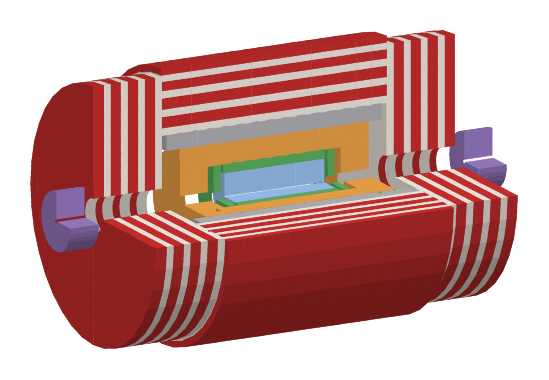
\begin{tikzpicture}
\begin{scope}[x=1cm,y=1cm,scale=0.245]
% written by example/G4/Standalone/draw_cms3d.py (do not edit): the CMS detector of Run 3, the quadrant x > 0, y > 0 cut away,
% 6639 quads sorted from back to front; 1 unit = 1 m times the scale of the enclosing scope
\begin{scope}[line width=0.15pt, line join=round, c/.style args={#1/#2/#3}{fill={rgb,255:red,#1;green,#2;blue,#3},draw={rgb,255:red,#1;green,#2;blue,#3}}]
\filldraw[c=141/31/31](5.96,1.75)--(5.62,1.80)--(5.76,0.60)--(6.09,0.67)--cycle;
\filldraw[c=141/31/31](6.09,0.67)--(5.76,0.60)--(6.00,-0.58)--(6.31,-0.38)--cycle;
\filldraw[c=141/31/31](5.92,2.80)--(5.57,2.99)--(5.62,1.80)--(5.96,1.75)--cycle;
\filldraw[c=168/164/157](5.61,1.69)--(5.26,1.75)--(5.41,0.55)--(5.74,0.62)--cycle;
\filldraw[c=168/164/157](5.74,0.62)--(5.41,0.55)--(5.65,-0.63)--(5.96,-0.43)--cycle;
\filldraw[c=141/31/31](6.31,-0.38)--(6.00,-0.58)--(6.33,-1.70)--(6.60,-1.38)--cycle;
\filldraw[c=168/164/157](5.57,2.75)--(5.21,2.93)--(5.26,1.75)--(5.61,1.69)--cycle;
\filldraw[c=168/164/157](5.96,-0.43)--(5.65,-0.63)--(5.98,-1.76)--(6.25,-1.43)--cycle;
\filldraw[c=141/31/31](5.08,1.62)--(4.73,1.67)--(4.88,0.47)--(5.21,0.54)--cycle;
\filldraw[c=141/31/31](5.96,3.81)--(5.62,4.12)--(5.57,2.99)--(5.92,2.80)--cycle;
\filldraw[c=141/31/31](5.21,0.54)--(4.88,0.47)--(5.12,-0.71)--(5.43,-0.51)--cycle;
\filldraw[c=141/31/31](5.04,2.67)--(4.68,2.86)--(4.73,1.67)--(5.08,1.62)--cycle;
\filldraw[c=141/31/31](6.60,-1.38)--(6.33,-1.70)--(6.73,-2.74)--(6.96,-2.30)--cycle;
\filldraw[c=168/164/157](4.73,1.56)--(4.38,1.62)--(4.53,0.42)--(4.86,0.49)--cycle;
\filldraw[c=168/164/157](5.61,3.76)--(5.26,4.07)--(5.21,2.93)--(5.57,2.75)--cycle;
\filldraw[c=141/31/31](6.31,1.69)--(5.96,1.75)--(6.09,0.67)--(6.43,0.75)--cycle;
\filldraw[c=168/164/157](4.86,0.49)--(4.53,0.42)--(4.77,-0.76)--(5.07,-0.56)--cycle;
\filldraw[c=141/31/31](6.43,0.75)--(6.09,0.67)--(6.31,-0.38)--(6.61,-0.18)--cycle;
\filldraw[c=141/31/31](5.43,-0.51)--(5.12,-0.71)--(5.45,-1.83)--(5.72,-1.51)--cycle;
\filldraw[c=168/164/157](4.68,2.62)--(4.33,2.80)--(4.38,1.62)--(4.73,1.56)--cycle;
\filldraw[c=141/31/31](6.27,2.62)--(5.92,2.80)--(5.96,1.75)--(6.31,1.69)--cycle;
\filldraw[c=168/164/157](6.25,-1.43)--(5.98,-1.76)--(6.38,-2.79)--(6.61,-2.35)--cycle;
\filldraw[c=168/164/157](5.96,1.64)--(5.61,1.69)--(5.74,0.62)--(6.07,0.70)--cycle;
\filldraw[c=168/164/157](6.07,0.70)--(5.74,0.62)--(5.96,-0.43)--(6.26,-0.23)--cycle;
\filldraw[c=168/164/157](5.07,-0.56)--(4.77,-0.76)--(5.09,-1.89)--(5.36,-1.56)--cycle;
\filldraw[c=141/31/31](6.61,-0.18)--(6.31,-0.38)--(6.60,-1.38)--(6.87,-1.06)--cycle;
\filldraw[c=141/31/31](4.20,1.49)--(3.85,1.54)--(4.00,0.34)--(4.33,0.41)--cycle;
\filldraw[c=141/31/31](5.08,3.69)--(4.73,3.99)--(4.68,2.86)--(5.04,2.67)--cycle;
\filldraw[c=141/31/31](6.09,4.75)--(5.76,5.17)--(5.62,4.12)--(5.96,3.81)--cycle;
\filldraw[c=141/31/31](4.33,0.41)--(4.00,0.34)--(4.24,-0.84)--(4.54,-0.64)--cycle;
\filldraw[c=168/164/157](5.92,2.57)--(5.57,2.75)--(5.61,1.69)--(5.96,1.64)--cycle;
\filldraw[c=141/31/31](4.15,2.54)--(3.80,2.73)--(3.85,1.54)--(4.20,1.49)--cycle;
\filldraw[c=168/164/157](6.26,-0.23)--(5.96,-0.43)--(6.25,-1.43)--(6.52,-1.11)--cycle;
\filldraw[c=141/31/31](6.31,3.51)--(5.96,3.81)--(5.92,2.80)--(6.27,2.62)--cycle;
\filldraw[c=141/31/31](5.72,-1.51)--(5.45,-1.83)--(5.85,-2.87)--(6.08,-2.43)--cycle;
\filldraw[c=168/164/157](3.84,1.43)--(3.50,1.49)--(3.64,0.29)--(3.98,0.36)--cycle;
\filldraw[c=168/164/157](4.73,3.63)--(4.38,3.94)--(4.33,2.80)--(4.68,2.62)--cycle;
\filldraw[c=168/164/157](5.74,4.70)--(5.41,5.12)--(5.26,4.07)--(5.61,3.76)--cycle;
\filldraw[c=141/31/31](5.43,1.56)--(5.08,1.62)--(5.21,0.54)--(5.54,0.62)--cycle;
\filldraw[c=168/164/157](3.98,0.36)--(3.64,0.29)--(3.88,-0.89)--(4.19,-0.69)--cycle;
\filldraw[c=141/31/31](5.54,0.62)--(5.21,0.54)--(5.43,-0.51)--(5.73,-0.31)--cycle;
\filldraw[c=141/31/31](4.54,-0.64)--(4.24,-0.84)--(4.56,-1.96)--(4.83,-1.64)--cycle;
\filldraw[c=141/31/31](6.96,-2.30)--(6.73,-2.74)--(7.20,-3.65)--(7.37,-3.11)--cycle;
\filldraw[c=141/31/31](6.87,-1.06)--(6.60,-1.38)--(6.96,-2.30)--(7.18,-1.87)--cycle;
\filldraw[c=168/164/157](3.80,2.49)--(3.45,2.67)--(3.50,1.49)--(3.84,1.43)--cycle;
\filldraw[c=141/31/31](5.39,2.49)--(5.04,2.67)--(5.08,1.62)--(5.43,1.56)--cycle;
\filldraw[c=168/164/157](5.96,3.46)--(5.61,3.76)--(5.57,2.75)--(5.92,2.57)--cycle;
\filldraw[c=168/164/157](5.36,-1.56)--(5.09,-1.89)--(5.50,-2.92)--(5.72,-2.48)--cycle;
\filldraw[c=168/164/157](5.07,1.51)--(4.73,1.56)--(4.86,0.49)--(5.19,0.57)--cycle;
\filldraw[c=168/164/157](5.19,0.57)--(4.86,0.49)--(5.07,-0.56)--(5.38,-0.36)--cycle;
\filldraw[c=168/164/157](4.19,-0.69)--(3.88,-0.89)--(4.21,-2.02)--(4.48,-1.69)--cycle;
\filldraw[c=141/31/31](6.66,1.64)--(6.31,1.69)--(6.43,0.75)--(6.76,0.82)--cycle;
\filldraw[c=141/31/31](5.73,-0.31)--(5.43,-0.51)--(5.72,-1.51)--(5.99,-1.19)--cycle;
\filldraw[c=168/164/157](6.61,-2.35)--(6.38,-2.79)--(6.84,-3.70)--(7.02,-3.16)--cycle;
\filldraw[c=141/31/31](3.31,1.36)--(2.97,1.41)--(3.11,0.21)--(3.45,0.29)--cycle;
\filldraw[c=141/31/31](4.20,3.56)--(3.85,3.86)--(3.80,2.73)--(4.15,2.54)--cycle;
\filldraw[c=141/31/31](6.76,0.82)--(6.43,0.75)--(6.61,-0.18)--(6.92,0.03)--cycle;
\filldraw[c=141/31/31](5.21,4.62)--(4.88,5.04)--(4.73,3.99)--(5.08,3.69)--cycle;
\filldraw[c=141/31/31](3.45,0.29)--(3.11,0.21)--(3.35,-0.97)--(3.66,-0.77)--cycle;
\filldraw[c=168/164/157](6.52,-1.11)--(6.25,-1.43)--(6.61,-2.35)--(6.83,-1.92)--cycle;
\filldraw[c=168/164/157](5.03,2.44)--(4.68,2.62)--(4.73,1.56)--(5.07,1.51)--cycle;
\filldraw[c=141/31/31](6.62,2.44)--(6.27,2.62)--(6.31,1.69)--(6.66,1.64)--cycle;
\filldraw[c=141/31/31](6.43,4.33)--(6.09,4.75)--(5.96,3.81)--(6.31,3.51)--cycle;
\filldraw[c=141/31/31](3.27,2.41)--(2.92,2.60)--(2.97,1.41)--(3.31,1.36)--cycle;
\filldraw[c=168/164/157](6.30,1.58)--(5.96,1.64)--(6.07,0.70)--(6.40,0.77)--cycle;
\filldraw[c=168/164/157](5.38,-0.36)--(5.07,-0.56)--(5.36,-1.56)--(5.63,-1.24)--cycle;
\filldraw[c=141/31/31](5.43,3.38)--(5.08,3.69)--(5.04,2.67)--(5.39,2.49)--cycle;
\filldraw[c=141/31/31](6.92,0.03)--(6.61,-0.18)--(6.87,-1.06)--(7.14,-0.73)--cycle;
\filldraw[c=141/31/31](4.83,-1.64)--(4.56,-1.96)--(4.97,-3.00)--(5.19,-2.56)--cycle;
\filldraw[c=168/164/157](2.96,1.31)--(2.61,1.36)--(2.76,0.16)--(3.09,0.23)--cycle;
\filldraw[c=168/164/157](3.84,3.50)--(3.50,3.81)--(3.45,2.67)--(3.80,2.49)--cycle;
\filldraw[c=168/164/157](6.40,0.77)--(6.07,0.70)--(6.26,-0.23)--(6.57,-0.03)--cycle;
\filldraw[c=141/31/31](6.31,5.58)--(6.00,6.10)--(5.76,5.17)--(6.09,4.75)--cycle;
\filldraw[c=168/164/157](4.86,4.57)--(4.53,4.99)--(4.38,3.94)--(4.73,3.63)--cycle;
\filldraw[c=141/31/31](4.54,1.43)--(4.20,1.49)--(4.33,0.41)--(4.66,0.49)--cycle;
\filldraw[c=168/164/157](3.09,0.23)--(2.76,0.16)--(3.00,-1.02)--(3.31,-0.82)--cycle;
\filldraw[c=141/31/31](4.66,0.49)--(4.33,0.41)--(4.54,-0.64)--(4.85,-0.44)--cycle;
\filldraw[c=141/31/31](3.66,-0.77)--(3.35,-0.97)--(3.68,-2.09)--(3.95,-1.77)--cycle;
\filldraw[c=141/31/31](6.08,-2.43)--(5.85,-2.87)--(6.32,-3.78)--(6.49,-3.24)--cycle;
\filldraw[c=168/164/157](6.27,2.39)--(5.92,2.57)--(5.96,1.64)--(6.30,1.58)--cycle;
\filldraw[c=168/164/157](6.07,4.28)--(5.74,4.70)--(5.61,3.76)--(5.96,3.46)--cycle;
\filldraw[c=141/31/31](5.99,-1.19)--(5.72,-1.51)--(6.08,-2.43)--(6.30,-2.00)--cycle;
\filldraw[c=168/164/157](2.92,2.36)--(2.56,2.55)--(2.61,1.36)--(2.96,1.31)--cycle;
\filldraw[c=141/31/31](6.66,3.21)--(6.31,3.51)--(6.27,2.62)--(6.62,2.44)--cycle;
\filldraw[c=141/31/31](4.50,2.36)--(4.15,2.54)--(4.20,1.49)--(4.54,1.43)--cycle;
\filldraw[c=168/164/157](5.07,3.33)--(4.73,3.63)--(4.68,2.62)--(5.03,2.44)--cycle;
\filldraw[c=141/31/31](7.18,-1.87)--(6.96,-2.30)--(7.37,-3.11)--(7.55,-2.58)--cycle;
\filldraw[c=168/164/157](6.57,-0.03)--(6.26,-0.23)--(6.52,-1.11)--(6.79,-0.79)--cycle;
\filldraw[c=168/164/157](4.48,-1.69)--(4.21,-2.02)--(4.61,-3.05)--(4.84,-2.61)--cycle;
\filldraw[c=168/164/157](5.96,5.53)--(5.65,6.05)--(5.41,5.12)--(5.74,4.70)--cycle;
\filldraw[c=168/164/157](4.19,1.38)--(3.84,1.43)--(3.98,0.36)--(4.31,0.44)--cycle;
\filldraw[c=168/164/157](4.31,0.44)--(3.98,0.36)--(4.19,-0.69)--(4.49,-0.49)--cycle;
\filldraw[c=168/164/157](3.31,-0.82)--(3.00,-1.02)--(3.33,-2.14)--(3.60,-1.82)--cycle;
\filldraw[c=141/31/31](5.77,1.51)--(5.43,1.56)--(5.54,0.62)--(5.87,0.69)--cycle;
\filldraw[c=141/31/31](4.85,-0.44)--(4.54,-0.64)--(4.83,-1.64)--(5.10,-1.32)--cycle;
\filldraw[c=168/164/157](5.72,-2.48)--(5.50,-2.92)--(5.96,-3.83)--(6.14,-3.29)--cycle;
\filldraw[c=141/31/31](3.31,3.43)--(2.97,3.73)--(2.92,2.60)--(3.27,2.41)--cycle;
\filldraw[c=141/31/31](5.87,0.69)--(5.54,0.62)--(5.73,-0.31)--(6.04,-0.10)--cycle;
\filldraw[c=141/31/31](7.14,-0.73)--(6.87,-1.06)--(7.18,-1.87)--(7.41,-1.43)--cycle;
\filldraw[c=141/31/31](4.33,4.49)--(4.00,4.91)--(3.85,3.86)--(4.20,3.56)--cycle;
\filldraw[c=141/31/31](7.37,-3.11)--(7.20,-3.65)--(7.71,-4.41)--(7.83,-3.79)--cycle;
\filldraw[c=168/164/157](5.63,-1.24)--(5.36,-1.56)--(5.72,-2.48)--(5.95,-2.05)--cycle;
\filldraw[c=168/164/157](6.30,3.15)--(5.96,3.46)--(5.92,2.57)--(6.27,2.39)--cycle;
\filldraw[c=168/164/157](4.15,2.31)--(3.80,2.49)--(3.84,1.43)--(4.19,1.38)--cycle;
\filldraw[c=168/164/157](6.83,-1.92)--(6.61,-2.35)--(7.02,-3.16)--(7.20,-2.63)--cycle;
\filldraw[c=141/31/31](5.74,2.31)--(5.39,2.49)--(5.43,1.56)--(5.77,1.51)--cycle;
\filldraw[c=141/31/31](5.54,4.20)--(5.21,4.62)--(5.08,3.69)--(5.43,3.38)--cycle;
\filldraw[c=168/164/157](5.42,1.45)--(5.07,1.51)--(5.19,0.57)--(5.52,0.64)--cycle;
\filldraw[c=168/164/157](4.49,-0.49)--(4.19,-0.69)--(4.48,-1.69)--(4.75,-1.37)--cycle;
\filldraw[c=141/31/31](4.54,3.25)--(4.20,3.56)--(4.15,2.54)--(4.50,2.36)--cycle;
\filldraw[c=141/31/31](6.04,-0.10)--(5.73,-0.31)--(5.99,-1.19)--(6.26,-0.86)--cycle;
\filldraw[c=141/31/31](3.95,-1.77)--(3.68,-2.09)--(4.08,-3.12)--(4.31,-2.69)--cycle;
\filldraw[c=168/164/157](2.96,3.37)--(2.61,3.68)--(2.56,2.55)--(2.92,2.36)--cycle;
\filldraw[c=168/164/157](5.52,0.64)--(5.19,0.57)--(5.38,-0.36)--(5.68,-0.16)--cycle;
\filldraw[c=141/31/31](7.00,1.58)--(6.66,1.64)--(6.76,0.82)--(7.09,0.90)--cycle;
\filldraw[c=168/164/157](6.79,-0.79)--(6.52,-1.11)--(6.83,-1.92)--(7.06,-1.48)--cycle;
\filldraw[c=141/31/31](5.43,5.45)--(5.12,5.97)--(4.88,5.04)--(5.21,4.62)--cycle;
\filldraw[c=168/164/157](3.98,4.44)--(3.64,4.86)--(3.50,3.81)--(3.84,3.50)--cycle;
\filldraw[c=141/31/31](3.66,1.30)--(3.31,1.36)--(3.45,0.29)--(3.78,0.36)--cycle;
\filldraw[c=141/31/31](7.09,0.90)--(6.76,0.82)--(6.92,0.03)--(7.22,0.23)--cycle;
\filldraw[c=168/164/157](7.02,-3.16)--(6.84,-3.70)--(7.36,-4.46)--(7.48,-3.84)--cycle;
\filldraw[c=141/31/31](6.61,5.06)--(6.31,5.58)--(6.09,4.75)--(6.43,4.33)--cycle;
\filldraw[c=141/31/31](3.78,0.36)--(3.45,0.29)--(3.66,-0.77)--(3.96,-0.56)--cycle;
\filldraw[c=141/31/31](6.76,3.91)--(6.43,4.33)--(6.31,3.51)--(6.66,3.21)--cycle;
\filldraw[c=141/31/31](5.19,-2.56)--(4.97,-3.00)--(5.43,-3.90)--(5.61,-3.37)--cycle;
\filldraw[c=168/164/157](5.39,2.26)--(5.03,2.44)--(5.07,1.51)--(5.42,1.45)--cycle;
\filldraw[c=141/31/31](6.98,2.26)--(6.62,2.44)--(6.66,1.64)--(7.00,1.58)--cycle;
\filldraw[c=168/164/157](5.19,4.15)--(4.86,4.57)--(4.73,3.63)--(5.07,3.33)--cycle;
\filldraw[c=141/31/31](5.10,-1.32)--(4.83,-1.64)--(5.19,-2.56)--(5.42,-2.13)--cycle;
\filldraw[c=141/31/31](5.77,3.08)--(5.43,3.38)--(5.39,2.49)--(5.74,2.31)--cycle;
\filldraw[c=141/31/31](3.62,2.23)--(3.27,2.41)--(3.31,1.36)--(3.66,1.30)--cycle;
\filldraw[c=168/164/157](4.19,3.20)--(3.84,3.50)--(3.80,2.49)--(4.15,2.31)--cycle;
\filldraw[c=141/31/31](6.30,-2.00)--(6.08,-2.43)--(6.49,-3.24)--(6.67,-2.71)--cycle;
\filldraw[c=168/164/157](5.68,-0.16)--(5.38,-0.36)--(5.63,-1.24)--(5.90,-0.91)--cycle;
\filldraw[c=141/31/31](7.22,0.23)--(6.92,0.03)--(7.14,-0.73)--(7.41,-0.41)--cycle;
\filldraw[c=168/164/157](3.60,-1.82)--(3.33,-2.14)--(3.73,-3.18)--(3.96,-2.74)--cycle;
\filldraw[c=168/164/157](6.65,1.53)--(6.30,1.58)--(6.40,0.77)--(6.73,0.85)--cycle;
\filldraw[c=168/164/157](5.07,5.40)--(4.77,5.92)--(4.53,4.99)--(4.86,4.57)--cycle;
\filldraw[c=168/164/157](3.31,1.25)--(2.96,1.31)--(3.09,0.23)--(3.42,0.31)--cycle;
\filldraw[c=168/164/157](6.73,0.85)--(6.40,0.77)--(6.57,-0.03)--(6.87,0.18)--cycle;
\filldraw[c=168/164/157](6.26,5.01)--(5.96,5.53)--(5.74,4.70)--(6.07,4.28)--cycle;
\filldraw[c=168/164/157](3.42,0.31)--(3.09,0.23)--(3.31,-0.82)--(3.61,-0.62)--cycle;
\filldraw[c=168/164/157](6.40,3.86)--(6.07,4.28)--(5.96,3.46)--(6.30,3.15)--cycle;
\filldraw[c=141/31/31](4.89,1.38)--(4.54,1.43)--(4.66,0.49)--(4.99,0.56)--cycle;
\filldraw[c=141/31/31](7.41,-1.43)--(7.18,-1.87)--(7.55,-2.58)--(7.73,-2.05)--cycle;
\filldraw[c=141/31/31](3.96,-0.56)--(3.66,-0.77)--(3.95,-1.77)--(4.22,-1.45)--cycle;
\filldraw[c=168/164/157](4.84,-2.61)--(4.61,-3.05)--(5.08,-3.96)--(5.26,-3.42)--cycle;
\filldraw[c=141/31/31](4.99,0.56)--(4.66,0.49)--(4.85,-0.44)--(5.15,-0.23)--cycle;
\filldraw[c=141/31/31](6.26,-0.86)--(5.99,-1.19)--(6.30,-2.00)--(6.53,-1.56)--cycle;
\filldraw[c=168/164/157](6.62,2.20)--(6.27,2.39)--(6.30,1.58)--(6.65,1.53)--cycle;
\filldraw[c=141/31/31](3.45,4.36)--(3.11,4.78)--(2.97,3.73)--(3.31,3.43)--cycle;
\filldraw[c=141/31/31](7.00,2.90)--(6.66,3.21)--(6.62,2.44)--(6.98,2.26)--cycle;
\filldraw[c=141/31/31](6.49,-3.24)--(6.32,-3.78)--(6.83,-4.53)--(6.95,-3.92)--cycle;
\filldraw[c=141/31/31](7.55,-2.58)--(7.37,-3.11)--(7.83,-3.79)--(7.95,-3.18)--cycle;
\filldraw[c=168/164/157](4.75,-1.37)--(4.48,-1.69)--(4.84,-2.61)--(5.07,-2.18)--cycle;
\filldraw[c=168/164/157](5.42,3.02)--(5.07,3.33)--(5.03,2.44)--(5.39,2.26)--cycle;
\filldraw[c=141/31/31](6.60,6.28)--(6.33,6.88)--(6.00,6.10)--(6.31,5.58)--cycle;
\filldraw[c=168/164/157](3.27,2.18)--(2.92,2.36)--(2.96,1.31)--(3.31,1.25)--cycle;
\filldraw[c=168/164/157](5.95,-2.05)--(5.72,-2.48)--(6.14,-3.29)--(6.31,-2.76)--cycle;
\filldraw[c=168/164/157](6.87,0.18)--(6.57,-0.03)--(6.79,-0.79)--(7.06,-0.46)--cycle;
\filldraw[c=141/31/31](4.86,2.18)--(4.50,2.36)--(4.54,1.43)--(4.89,1.38)--cycle;
\filldraw[c=141/31/31](4.66,4.07)--(4.33,4.49)--(4.20,3.56)--(4.54,3.25)--cycle;
\filldraw[c=141/31/31](7.41,-0.41)--(7.14,-0.73)--(7.41,-1.43)--(7.64,-1.00)--cycle;
\filldraw[c=168/164/157](4.54,1.33)--(4.19,1.38)--(4.31,0.44)--(4.64,0.51)--cycle;
\filldraw[c=168/164/157](7.06,-1.48)--(6.83,-1.92)--(7.20,-2.63)--(7.37,-2.10)--cycle;
\filldraw[c=168/164/157](3.61,-0.62)--(3.31,-0.82)--(3.60,-1.82)--(3.87,-1.50)--cycle;
\filldraw[c=141/31/31](3.66,3.12)--(3.31,3.43)--(3.27,2.41)--(3.62,2.23)--cycle;
\filldraw[c=141/31/31](5.15,-0.23)--(4.85,-0.44)--(5.10,-1.32)--(5.37,-0.99)--cycle;
\filldraw[c=168/164/157](4.64,0.51)--(4.31,0.44)--(4.49,-0.49)--(4.80,-0.28)--cycle;
\filldraw[c=141/31/31](6.12,1.45)--(5.77,1.51)--(5.87,0.69)--(6.20,0.77)--cycle;
\filldraw[c=168/164/157](5.90,-0.91)--(5.63,-1.24)--(5.95,-2.05)--(6.18,-1.61)--cycle;
\filldraw[c=141/31/31](4.54,5.32)--(4.24,5.84)--(4.00,4.91)--(4.33,4.49)--cycle;
\filldraw[c=168/164/157](3.09,4.31)--(2.76,4.73)--(2.61,3.68)--(2.96,3.37)--cycle;
\filldraw[c=141/31/31](6.20,0.77)--(5.87,0.69)--(6.04,-0.10)--(6.34,0.10)--cycle;
\filldraw[c=168/164/157](6.65,2.85)--(6.30,3.15)--(6.27,2.39)--(6.62,2.20)--cycle;
\filldraw[c=168/164/157](6.14,-3.29)--(5.96,-3.83)--(6.48,-4.59)--(6.60,-3.97)--cycle;
\filldraw[c=168/164/157](7.20,-2.63)--(7.02,-3.16)--(7.48,-3.84)--(7.60,-3.23)--cycle;
\filldraw[c=168/164/157](6.25,6.23)--(5.98,6.83)--(5.65,6.05)--(5.96,5.53)--cycle;
\filldraw[c=141/31/31](5.73,4.93)--(5.43,5.45)--(5.21,4.62)--(5.54,4.20)--cycle;
\filldraw[c=141/31/31](5.87,3.78)--(5.54,4.20)--(5.43,3.38)--(5.77,3.08)--cycle;
\filldraw[c=141/31/31](4.31,-2.69)--(4.08,-3.12)--(4.55,-4.03)--(4.73,-3.50)--cycle;
\filldraw[c=168/164/157](4.50,2.13)--(4.15,2.31)--(4.19,1.38)--(4.54,1.33)--cycle;
\filldraw[c=141/31/31](6.92,4.54)--(6.61,5.06)--(6.43,4.33)--(6.76,3.91)--cycle;
\filldraw[c=141/31/31](6.09,2.13)--(5.74,2.31)--(5.77,1.51)--(6.12,1.45)--cycle;
\filldraw[c=168/164/157](4.31,4.02)--(3.98,4.44)--(3.84,3.50)--(4.19,3.20)--cycle;
\filldraw[c=141/31/31](4.22,-1.45)--(3.95,-1.77)--(4.31,-2.69)--(4.54,-2.25)--cycle;
\filldraw[c=141/31/31](4.89,2.95)--(4.54,3.25)--(4.50,2.36)--(4.86,2.18)--cycle;
\filldraw[c=168/164/157](7.06,-0.46)--(6.79,-0.79)--(7.06,-1.48)--(7.28,-1.05)--cycle;
\filldraw[c=168/164/157](3.31,3.07)--(2.96,3.37)--(2.92,2.36)--(3.27,2.18)--cycle;
\filldraw[c=141/31/31](5.42,-2.13)--(5.19,-2.56)--(5.61,-3.37)--(5.78,-2.84)--cycle;
\filldraw[c=168/164/157](4.80,-0.28)--(4.49,-0.49)--(4.75,-1.37)--(5.02,-1.04)--cycle;
\filldraw[c=141/31/31](6.34,0.10)--(6.04,-0.10)--(6.26,-0.86)--(6.53,-0.54)--cycle;
\filldraw[c=141/31/31](7.09,3.50)--(6.76,3.91)--(6.66,3.21)--(7.00,2.90)--cycle;
\filldraw[c=168/164/157](5.77,1.40)--(5.42,1.45)--(5.52,0.64)--(5.85,0.72)--cycle;
\filldraw[c=168/164/157](4.19,5.27)--(3.88,5.79)--(3.64,4.86)--(3.98,4.44)--cycle;
\filldraw[c=168/164/157](5.85,0.72)--(5.52,0.64)--(5.68,-0.16)--(5.99,0.05)--cycle;
\filldraw[c=141/31/31](7.83,-3.79)--(7.71,-4.41)--(8.26,-4.99)--(8.32,-4.31)--cycle;
\filldraw[c=141/31/31](7.35,1.53)--(7.00,1.58)--(7.09,0.90)--(7.42,0.97)--cycle;
\filldraw[c=168/164/157](5.38,4.88)--(5.07,5.40)--(4.86,4.57)--(5.19,4.15)--cycle;
\filldraw[c=141/31/31](7.42,0.97)--(7.09,0.90)--(7.22,0.23)--(7.53,0.43)--cycle;
\filldraw[c=168/164/157](5.52,3.73)--(5.19,4.15)--(5.07,3.33)--(5.42,3.02)--cycle;
\filldraw[c=141/31/31](4.01,1.25)--(3.66,1.30)--(3.78,0.36)--(4.11,0.44)--cycle;
\filldraw[c=141/31/31](6.53,-1.56)--(6.30,-2.00)--(6.67,-2.71)--(6.84,-2.18)--cycle;
\filldraw[c=168/164/157](3.96,-2.74)--(3.73,-3.18)--(4.20,-4.09)--(4.37,-3.55)--cycle;
\filldraw[c=141/31/31](4.11,0.44)--(3.78,0.36)--(3.96,-0.56)--(4.27,-0.36)--cycle;
\filldraw[c=168/164/157](6.57,4.49)--(6.26,5.01)--(6.07,4.28)--(6.40,3.86)--cycle;
\filldraw[c=141/31/31](6.87,5.68)--(6.60,6.28)--(6.31,5.58)--(6.61,5.06)--cycle;
\filldraw[c=141/31/31](5.37,-0.99)--(5.10,-1.32)--(5.42,-2.13)--(5.65,-1.69)--cycle;
\filldraw[c=168/164/157](5.74,2.07)--(5.39,2.26)--(5.42,1.45)--(5.77,1.40)--cycle;
\filldraw[c=141/31/31](7.33,2.07)--(6.98,2.26)--(7.00,1.58)--(7.35,1.53)--cycle;
\filldraw[c=141/31/31](6.12,2.77)--(5.77,3.08)--(5.74,2.31)--(6.09,2.13)--cycle;
\filldraw[c=141/31/31](5.61,-3.37)--(5.43,-3.90)--(5.95,-4.66)--(6.07,-4.05)--cycle;
\filldraw[c=141/31/31](6.67,-2.71)--(6.49,-3.24)--(6.95,-3.92)--(7.07,-3.30)--cycle;
\filldraw[c=168/164/157](3.87,-1.50)--(3.60,-1.82)--(3.96,-2.74)--(4.18,-2.31)--cycle;
\filldraw[c=141/31/31](7.73,-2.05)--(7.55,-2.58)--(7.95,-3.18)--(8.07,-2.56)--cycle;
\filldraw[c=141/31/31](7.64,-1.00)--(7.41,-1.43)--(7.73,-2.05)--(7.90,-1.51)--cycle;
\filldraw[c=168/164/157](4.54,2.89)--(4.19,3.20)--(4.15,2.31)--(4.50,2.13)--cycle;
\filldraw[c=141/31/31](5.72,6.15)--(5.45,6.75)--(5.12,5.97)--(5.43,5.45)--cycle;
\filldraw[c=168/164/157](5.07,-2.18)--(4.84,-2.61)--(5.26,-3.42)--(5.43,-2.89)--cycle;
\filldraw[c=168/164/157](5.99,0.05)--(5.68,-0.16)--(5.90,-0.91)--(6.17,-0.59)--cycle;
\filldraw[c=168/164/157](6.73,3.44)--(6.40,3.86)--(6.30,3.15)--(6.65,2.85)--cycle;
\filldraw[c=141/31/31](3.97,2.05)--(3.62,2.23)--(3.66,1.30)--(4.01,1.25)--cycle;
\filldraw[c=141/31/31](7.53,0.43)--(7.22,0.23)--(7.41,-0.41)--(7.68,-0.09)--cycle;
\filldraw[c=168/164/157](7.48,-3.84)--(7.36,-4.46)--(7.91,-5.04)--(7.97,-4.36)--cycle;
\filldraw[c=168/164/157](7.00,1.48)--(6.65,1.53)--(6.73,0.85)--(7.06,0.92)--cycle;
\filldraw[c=141/31/31](3.78,3.94)--(3.45,4.36)--(3.31,3.43)--(3.66,3.12)--cycle;
\filldraw[c=141/31/31](6.53,-0.54)--(6.26,-0.86)--(6.53,-1.56)--(6.75,-1.13)--cycle;
\filldraw[c=168/164/157](7.06,0.92)--(6.73,0.85)--(6.87,0.18)--(7.18,0.38)--cycle;
\filldraw[c=168/164/157](3.65,1.20)--(3.31,1.25)--(3.42,0.31)--(3.75,0.38)--cycle;
\filldraw[c=168/164/157](6.18,-1.61)--(5.95,-2.05)--(6.31,-2.76)--(6.49,-2.23)--cycle;
\filldraw[c=141/31/31](4.27,-0.36)--(3.96,-0.56)--(4.22,-1.45)--(4.49,-1.12)--cycle;
\filldraw[c=168/164/157](3.75,0.38)--(3.42,0.31)--(3.61,-0.62)--(3.92,-0.41)--cycle;
\filldraw[c=141/31/31](5.24,1.32)--(4.89,1.38)--(4.99,0.56)--(5.32,0.64)--cycle;
\filldraw[c=168/164/157](6.52,5.63)--(6.25,6.23)--(5.96,5.53)--(6.26,5.01)--cycle;
\filldraw[c=168/164/157](5.02,-1.04)--(4.75,-1.37)--(5.07,-2.18)--(5.29,-1.74)--cycle;
\filldraw[c=141/31/31](7.35,2.60)--(7.00,2.90)--(6.98,2.26)--(7.33,2.07)--cycle;
\filldraw[c=141/31/31](3.66,5.19)--(3.35,5.71)--(3.11,4.78)--(3.45,4.36)--cycle;
\filldraw[c=168/164/157](6.97,2.02)--(6.62,2.20)--(6.65,1.53)--(7.00,1.48)--cycle;
\filldraw[c=141/31/31](5.32,0.64)--(4.99,0.56)--(5.15,-0.23)--(5.46,-0.03)--cycle;
\filldraw[c=168/164/157](5.77,2.72)--(5.42,3.02)--(5.39,2.26)--(5.74,2.07)--cycle;
\filldraw[c=168/164/157](5.26,-3.42)--(5.08,-3.96)--(5.59,-4.72)--(5.71,-4.10)--cycle;
\filldraw[c=168/164/157](6.31,-2.76)--(6.14,-3.29)--(6.60,-3.97)--(6.72,-3.36)--cycle;
\filldraw[c=168/164/157](7.37,-2.10)--(7.20,-2.63)--(7.60,-3.23)--(7.72,-2.61)--cycle;
\filldraw[c=168/164/157](7.28,-1.05)--(7.06,-1.48)--(7.37,-2.10)--(7.55,-1.57)--cycle;
\filldraw[c=168/164/157](5.36,6.10)--(5.09,6.70)--(4.77,5.92)--(5.07,5.40)--cycle;
\filldraw[c=141/31/31](4.85,4.80)--(4.54,5.32)--(4.33,4.49)--(4.66,4.07)--cycle;
\filldraw[c=141/31/31](4.99,3.66)--(4.66,4.07)--(4.54,3.25)--(4.89,2.95)--cycle;
\filldraw[c=168/164/157](3.62,2.00)--(3.27,2.18)--(3.31,1.25)--(3.65,1.20)--cycle;
\filldraw[c=168/164/157](7.18,0.38)--(6.87,0.18)--(7.06,-0.46)--(7.33,-0.14)--cycle;
\filldraw[c=141/31/31](6.04,4.41)--(5.73,4.93)--(5.54,4.20)--(5.87,3.78)--cycle;
\filldraw[c=141/31/31](5.21,2.00)--(4.86,2.18)--(4.89,1.38)--(5.24,1.32)--cycle;
\filldraw[c=141/31/31](7.68,-0.09)--(7.41,-0.41)--(7.64,-1.00)--(7.86,-0.56)--cycle;
\filldraw[c=141/31/31](7.95,-3.18)--(7.83,-3.79)--(8.32,-4.31)--(8.39,-3.63)--cycle;
\filldraw[c=141/31/31](7.22,4.03)--(6.92,4.54)--(6.76,3.91)--(7.09,3.50)--cycle;
\filldraw[c=168/164/157](3.42,3.89)--(3.09,4.31)--(2.96,3.37)--(3.31,3.07)--cycle;
\filldraw[c=141/31/31](4.01,2.82)--(3.66,3.12)--(3.62,2.23)--(3.97,2.05)--cycle;
\filldraw[c=168/164/157](6.17,-0.59)--(5.90,-0.91)--(6.18,-1.61)--(6.40,-1.18)--cycle;
\filldraw[c=141/31/31](4.54,-2.25)--(4.31,-2.69)--(4.73,-3.50)--(4.90,-2.97)--cycle;
\filldraw[c=168/164/157](3.92,-0.41)--(3.61,-0.62)--(3.87,-1.50)--(4.14,-1.17)--cycle;
\filldraw[c=141/31/31](5.46,-0.03)--(5.15,-0.23)--(5.37,-0.99)--(5.64,-0.67)--cycle;
\filldraw[c=141/31/31](6.20,3.37)--(5.87,3.78)--(5.77,3.08)--(6.12,2.77)--cycle;
\filldraw[c=168/164/157](4.88,1.27)--(4.54,1.33)--(4.64,0.51)--(4.97,0.59)--cycle;
\filldraw[c=168/164/157](7.00,2.54)--(6.65,2.85)--(6.62,2.20)--(6.97,2.02)--cycle;
\filldraw[c=168/164/157](3.31,5.14)--(3.00,5.66)--(2.76,4.73)--(3.09,4.31)--cycle;
\filldraw[c=168/164/157](4.97,0.59)--(4.64,0.51)--(4.80,-0.28)--(5.10,-0.08)--cycle;
\filldraw[c=141/31/31](6.95,-3.92)--(6.83,-4.53)--(7.38,-5.12)--(7.44,-4.44)--cycle;
\filldraw[c=141/31/31](6.47,1.40)--(6.12,1.45)--(6.20,0.77)--(6.53,0.84)--cycle;
\filldraw[c=141/31/31](7.14,5.07)--(6.87,5.68)--(6.61,5.06)--(6.92,4.54)--cycle;
\filldraw[c=168/164/157](4.49,4.75)--(4.19,5.27)--(3.98,4.44)--(4.31,4.02)--cycle;
\filldraw[c=141/31/31](6.53,0.84)--(6.20,0.77)--(6.34,0.10)--(6.65,0.30)--cycle;
\filldraw[c=168/164/157](4.64,3.60)--(4.31,4.02)--(4.19,3.20)--(4.54,2.89)--cycle;
\filldraw[c=141/31/31](5.65,-1.69)--(5.42,-2.13)--(5.78,-2.84)--(5.96,-2.31)--cycle;
\filldraw[c=168/164/157](5.68,4.36)--(5.38,4.88)--(5.19,4.15)--(5.52,3.73)--cycle;
\filldraw[c=141/31/31](5.99,5.55)--(5.72,6.15)--(5.43,5.45)--(5.73,4.93)--cycle;
\filldraw[c=141/31/31](4.49,-1.12)--(4.22,-1.45)--(4.54,-2.25)--(4.76,-1.82)--cycle;
\filldraw[c=141/31/31](7.42,3.08)--(7.09,3.50)--(7.00,2.90)--(7.35,2.60)--cycle;
\filldraw[c=168/164/157](4.86,1.94)--(4.50,2.13)--(4.54,1.33)--(4.88,1.27)--cycle;
\filldraw[c=141/31/31](6.96,6.83)--(6.73,7.50)--(6.33,6.88)--(6.60,6.28)--cycle;
\filldraw[c=168/164/157](7.33,-0.14)--(7.06,-0.46)--(7.28,-1.05)--(7.51,-0.61)--cycle;
\filldraw[c=141/31/31](6.44,1.94)--(6.09,2.13)--(6.12,1.45)--(6.47,1.40)--cycle;
\filldraw[c=168/164/157](7.60,-3.23)--(7.48,-3.84)--(7.97,-4.36)--(8.03,-3.69)--cycle;
\filldraw[c=141/31/31](5.24,2.64)--(4.89,2.95)--(4.86,2.18)--(5.21,2.00)--cycle;
\filldraw[c=141/31/31](4.73,-3.50)--(4.55,-4.03)--(5.06,-4.79)--(5.19,-4.18)--cycle;
\filldraw[c=168/164/157](6.87,3.97)--(6.57,4.49)--(6.40,3.86)--(6.73,3.44)--cycle;
\filldraw[c=141/31/31](5.78,-2.84)--(5.61,-3.37)--(6.07,-4.05)--(6.19,-3.43)--cycle;
\filldraw[c=141/31/31](6.84,-2.18)--(6.67,-2.71)--(7.07,-3.30)--(7.19,-2.69)--cycle;
\filldraw[c=141/31/31](7.90,-1.51)--(7.73,-2.05)--(8.07,-2.56)--(8.20,-1.95)--cycle;
\filldraw[c=141/31/31](6.75,-1.13)--(6.53,-1.56)--(6.84,-2.18)--(7.02,-1.64)--cycle;
\filldraw[c=168/164/157](3.65,2.77)--(3.31,3.07)--(3.27,2.18)--(3.62,2.00)--cycle;
\filldraw[c=141/31/31](4.83,6.02)--(4.56,6.63)--(4.24,5.84)--(4.54,5.32)--cycle;
\filldraw[c=168/164/157](4.18,-2.31)--(3.96,-2.74)--(4.37,-3.55)--(4.55,-3.02)--cycle;
\filldraw[c=168/164/157](5.10,-0.08)--(4.80,-0.28)--(5.02,-1.04)--(5.29,-0.72)--cycle;
\filldraw[c=168/164/157](5.85,3.31)--(5.52,3.73)--(5.42,3.02)--(5.77,2.72)--cycle;
\filldraw[c=141/31/31](6.65,0.30)--(6.34,0.10)--(6.53,-0.54)--(6.80,-0.22)--cycle;
\filldraw[c=168/164/157](6.60,-3.97)--(6.48,-4.59)--(7.03,-5.17)--(7.09,-4.49)--cycle;
\filldraw[c=168/164/157](6.11,1.35)--(5.77,1.40)--(5.85,0.72)--(6.18,0.79)--cycle;
\filldraw[c=141/31/31](7.86,-0.56)--(7.64,-1.00)--(7.90,-1.51)--(8.08,-0.98)--cycle;
\filldraw[c=168/164/157](6.79,5.02)--(6.52,5.63)--(6.26,5.01)--(6.57,4.49)--cycle;
\filldraw[c=141/31/31](5.64,-0.67)--(5.37,-0.99)--(5.65,-1.69)--(5.87,-1.26)--cycle;
\filldraw[c=168/164/157](6.18,0.79)--(5.85,0.72)--(5.99,0.05)--(6.29,0.25)--cycle;
\filldraw[c=168/164/157](5.29,-1.74)--(5.07,-2.18)--(5.43,-2.89)--(5.61,-2.36)--cycle;
\filldraw[c=141/31/31](7.70,1.47)--(7.35,1.53)--(7.42,0.97)--(7.75,1.05)--cycle;
\filldraw[c=141/31/31](7.75,1.05)--(7.42,0.97)--(7.53,0.43)--(7.83,0.63)--cycle;
\filldraw[c=141/31/31](4.35,1.19)--(4.01,1.25)--(4.11,0.44)--(4.44,0.51)--cycle;
\filldraw[c=168/164/157](5.63,5.50)--(5.36,6.10)--(5.07,5.40)--(5.38,4.88)--cycle;
\filldraw[c=168/164/157](4.14,-1.17)--(3.87,-1.50)--(4.18,-2.31)--(4.41,-1.87)--cycle;
\filldraw[c=168/164/157](7.06,3.03)--(6.73,3.44)--(6.65,2.85)--(7.00,2.54)--cycle;
\filldraw[c=141/31/31](6.47,2.47)--(6.12,2.77)--(6.09,2.13)--(6.44,1.94)--cycle;
\filldraw[c=168/164/157](6.61,6.78)--(6.38,7.45)--(5.98,6.83)--(6.25,6.23)--cycle;
\filldraw[c=168/164/157](6.09,1.89)--(5.74,2.07)--(5.77,1.40)--(6.11,1.35)--cycle;
\filldraw[c=141/31/31](4.44,0.51)--(4.11,0.44)--(4.27,-0.36)--(4.57,-0.16)--cycle;
\filldraw[c=141/31/31](8.07,-2.56)--(7.95,-3.18)--(8.39,-3.63)--(8.45,-2.96)--cycle;
\filldraw[c=168/164/157](4.88,2.59)--(4.54,2.89)--(4.50,2.13)--(4.86,1.94)--cycle;
\filldraw[c=168/164/157](4.37,-3.55)--(4.20,-4.09)--(4.71,-4.85)--(4.83,-4.23)--cycle;
\filldraw[c=168/164/157](5.43,-2.89)--(5.26,-3.42)--(5.71,-4.10)--(5.84,-3.49)--cycle;
\filldraw[c=141/31/31](7.68,1.89)--(7.33,2.07)--(7.35,1.53)--(7.70,1.47)--cycle;
\filldraw[c=168/164/157](6.49,-2.23)--(6.31,-2.76)--(6.72,-3.36)--(6.84,-2.74)--cycle;
\filldraw[c=168/164/157](7.55,-1.57)--(7.37,-2.10)--(7.72,-2.61)--(7.84,-2.00)--cycle;
\filldraw[c=168/164/157](6.40,-1.18)--(6.18,-1.61)--(6.49,-2.23)--(6.67,-1.69)--cycle;
\filldraw[c=168/164/157](4.48,5.97)--(4.21,6.57)--(3.88,5.79)--(4.19,5.27)--cycle;
\filldraw[c=141/31/31](3.96,4.67)--(3.66,5.19)--(3.45,4.36)--(3.78,3.94)--cycle;
\filldraw[c=141/31/31](4.11,3.53)--(3.78,3.94)--(3.66,3.12)--(4.01,2.82)--cycle;
\filldraw[c=168/164/157](6.29,0.25)--(5.99,0.05)--(6.17,-0.59)--(6.44,-0.27)--cycle;
\filldraw[c=141/31/31](7.83,0.63)--(7.53,0.43)--(7.68,-0.09)--(7.95,0.24)--cycle;
\filldraw[c=141/31/31](5.15,4.28)--(4.85,4.80)--(4.66,4.07)--(4.99,3.66)--cycle;
\filldraw[c=141/31/31](4.33,1.87)--(3.97,2.05)--(4.01,1.25)--(4.35,1.19)--cycle;
\filldraw[c=141/31/31](6.80,-0.22)--(6.53,-0.54)--(6.75,-1.13)--(6.98,-0.69)--cycle;
\filldraw[c=141/31/31](7.07,-3.30)--(6.95,-3.92)--(7.44,-4.44)--(7.50,-3.76)--cycle;
\filldraw[c=141/31/31](6.34,3.90)--(6.04,4.41)--(5.87,3.78)--(6.20,3.37)--cycle;
\filldraw[c=168/164/157](7.51,-0.61)--(7.28,-1.05)--(7.55,-1.57)--(7.73,-1.03)--cycle;
\filldraw[c=141/31/31](7.18,6.16)--(6.96,6.83)--(6.60,6.28)--(6.87,5.68)--cycle;
\filldraw[c=168/164/157](5.29,-0.72)--(5.02,-1.04)--(5.29,-1.74)--(5.52,-1.31)--cycle;
\filldraw[c=168/164/157](7.34,1.42)--(7.00,1.48)--(7.06,0.92)--(7.40,1.00)--cycle;
\filldraw[c=141/31/31](7.53,3.51)--(7.22,4.03)--(7.09,3.50)--(7.42,3.08)--cycle;
\filldraw[c=141/31/31](4.57,-0.16)--(4.27,-0.36)--(4.49,-1.12)--(4.76,-0.80)--cycle;
\filldraw[c=141/31/31](5.32,3.24)--(4.99,3.66)--(4.89,2.95)--(5.24,2.64)--cycle;
\filldraw[c=141/31/31](7.41,4.47)--(7.14,5.07)--(6.92,4.54)--(7.22,4.03)--cycle;
\filldraw[c=168/164/157](7.40,1.00)--(7.06,0.92)--(7.18,0.38)--(7.48,0.58)--cycle;
\filldraw[c=141/31/31](7.70,2.29)--(7.35,2.60)--(7.33,2.07)--(7.68,1.89)--cycle;
\filldraw[c=168/164/157](4.00,1.14)--(3.65,1.20)--(3.75,0.38)--(4.08,0.46)--cycle;
\filldraw[c=168/164/157](6.11,2.41)--(5.77,2.72)--(5.74,2.07)--(6.09,1.89)--cycle;
\filldraw[c=141/31/31](8.32,-4.31)--(8.26,-4.99)--(8.83,-5.39)--(8.83,-4.67)--cycle;
\filldraw[c=168/164/157](4.08,0.46)--(3.75,0.38)--(3.92,-0.41)--(4.22,-0.21)--cycle;
\filldraw[c=141/31/31](6.07,-4.05)--(5.95,-4.66)--(6.50,-5.25)--(6.56,-4.57)--cycle;
\filldraw[c=168/164/157](7.72,-2.61)--(7.60,-3.23)--(8.03,-3.69)--(8.09,-3.01)--cycle;
\filldraw[c=141/31/31](5.58,1.27)--(5.24,1.32)--(5.32,0.64)--(5.65,0.71)--cycle;
\filldraw[c=168/164/157](7.33,1.84)--(6.97,2.02)--(7.00,1.48)--(7.34,1.42)--cycle;
\filldraw[c=141/31/31](6.26,4.94)--(5.99,5.55)--(5.73,4.93)--(6.04,4.41)--cycle;
\filldraw[c=168/164/157](3.61,4.62)--(3.31,5.14)--(3.09,4.31)--(3.42,3.89)--cycle;
\filldraw[c=141/31/31](5.65,0.71)--(5.32,0.64)--(5.46,-0.03)--(5.76,0.17)--cycle;
\filldraw[c=168/164/157](3.75,3.47)--(3.42,3.89)--(3.31,3.07)--(3.65,2.77)--cycle;
\filldraw[c=141/31/31](4.76,-1.82)--(4.54,-2.25)--(4.90,-2.97)--(5.08,-2.43)--cycle;
\filldraw[c=141/31/31](7.95,0.24)--(7.68,-0.09)--(7.86,-0.56)--(8.09,-0.13)--cycle;
\filldraw[c=168/164/157](7.48,0.58)--(7.18,0.38)--(7.33,-0.14)--(7.60,0.19)--cycle;
\filldraw[c=168/164/157](4.80,4.23)--(4.49,4.75)--(4.31,4.02)--(4.64,3.60)--cycle;
\filldraw[c=141/31/31](5.10,5.42)--(4.83,6.02)--(4.54,5.32)--(4.85,4.80)--cycle;
\filldraw[c=141/31/31](6.53,2.95)--(6.20,3.37)--(6.12,2.77)--(6.47,2.47)--cycle;
\filldraw[c=168/164/157](3.97,1.82)--(3.62,2.00)--(3.65,1.20)--(4.00,1.14)--cycle;
\filldraw[c=141/31/31](6.08,6.70)--(5.85,7.37)--(5.45,6.75)--(5.72,6.15)--cycle;
\filldraw[c=168/164/157](6.44,-0.27)--(6.17,-0.59)--(6.40,-1.18)--(6.63,-0.74)--cycle;
\filldraw[c=141/31/31](5.56,1.81)--(5.21,2.00)--(5.24,1.32)--(5.58,1.27)--cycle;
\filldraw[c=168/164/157](6.72,-3.36)--(6.60,-3.97)--(7.09,-4.49)--(7.15,-3.82)--cycle;
\filldraw[c=141/31/31](4.35,2.51)--(4.01,2.82)--(3.97,2.05)--(4.33,1.87)--cycle;
\filldraw[c=168/164/157](5.99,3.84)--(5.68,4.36)--(5.52,3.73)--(5.85,3.31)--cycle;
\filldraw[c=141/31/31](4.90,-2.97)--(4.73,-3.50)--(5.19,-4.18)--(5.31,-3.56)--cycle;
\filldraw[c=141/31/31](5.96,-2.31)--(5.78,-2.84)--(6.19,-3.43)--(6.31,-2.82)--cycle;
\filldraw[c=168/164/157](6.83,6.11)--(6.61,6.78)--(6.25,6.23)--(6.52,5.63)--cycle;
\filldraw[c=141/31/31](7.02,-1.64)--(6.84,-2.18)--(7.19,-2.69)--(7.31,-2.07)--cycle;
\filldraw[c=141/31/31](5.87,-1.26)--(5.65,-1.69)--(5.96,-2.31)--(6.14,-1.77)--cycle;
\filldraw[c=141/31/31](8.08,-0.98)--(7.90,-1.51)--(8.20,-1.95)--(8.32,-1.33)--cycle;
\filldraw[c=141/31/31](3.95,5.89)--(3.68,6.50)--(3.35,5.71)--(3.66,5.19)--cycle;
\filldraw[c=168/164/157](7.18,3.45)--(6.87,3.97)--(6.73,3.44)--(7.06,3.03)--cycle;
\filldraw[c=168/164/157](4.22,-0.21)--(3.92,-0.41)--(4.14,-1.17)--(4.41,-0.85)--cycle;
\filldraw[c=168/164/157](4.97,3.19)--(4.64,3.60)--(4.54,2.89)--(4.88,2.59)--cycle;
\filldraw[c=141/31/31](5.76,0.17)--(5.46,-0.03)--(5.64,-0.67)--(5.91,-0.35)--cycle;
\filldraw[c=168/164/157](7.06,4.42)--(6.79,5.02)--(6.57,4.49)--(6.87,3.97)--cycle;
\filldraw[c=168/164/157](7.34,2.24)--(7.00,2.54)--(6.97,2.02)--(7.33,1.84)--cycle;
\filldraw[c=141/31/31](7.75,2.66)--(7.42,3.08)--(7.35,2.60)--(7.70,2.29)--cycle;
\filldraw[c=168/164/157](7.97,-4.36)--(7.91,-5.04)--(8.48,-5.44)--(8.48,-4.72)--cycle;
\filldraw[c=168/164/157](5.71,-4.10)--(5.59,-4.72)--(6.14,-5.30)--(6.20,-4.62)--cycle;
\filldraw[c=141/31/31](8.20,-1.95)--(8.07,-2.56)--(8.45,-2.96)--(8.51,-2.28)--cycle;
\filldraw[c=168/164/157](5.23,1.22)--(4.88,1.27)--(4.97,0.59)--(5.30,0.66)--cycle;
\filldraw[c=141/31/31](6.98,-0.69)--(6.75,-1.13)--(7.02,-1.64)--(7.20,-1.11)--cycle;
\filldraw[c=168/164/157](5.90,4.89)--(5.63,5.50)--(5.38,4.88)--(5.68,4.36)--cycle;
\filldraw[c=141/31/31](4.76,-0.80)--(4.49,-1.12)--(4.76,-1.82)--(4.99,-1.38)--cycle;
\filldraw[c=168/164/157](5.30,0.66)--(4.97,0.59)--(5.10,-0.08)--(5.41,0.12)--cycle;
\filldraw[c=168/164/157](4.41,-1.87)--(4.18,-2.31)--(4.55,-3.02)--(4.72,-2.49)--cycle;
\filldraw[c=168/164/157](7.60,0.19)--(7.33,-0.14)--(7.51,-0.61)--(7.74,-0.18)--cycle;
\filldraw[c=141/31/31](6.81,1.34)--(6.47,1.40)--(6.53,0.84)--(6.87,0.92)--cycle;
\filldraw[c=141/31/31](7.41,5.49)--(7.18,6.16)--(6.87,5.68)--(7.14,5.07)--cycle;
\filldraw[c=141/31/31](6.87,0.92)--(6.53,0.84)--(6.65,0.30)--(6.95,0.50)--cycle;
\filldraw[c=168/164/157](4.75,5.37)--(4.48,5.97)--(4.19,5.27)--(4.49,4.75)--cycle;
\filldraw[c=168/164/157](6.18,2.90)--(5.85,3.31)--(5.77,2.72)--(6.11,2.41)--cycle;
\filldraw[c=141/31/31](5.58,2.34)--(5.24,2.64)--(5.21,2.00)--(5.56,1.81)--cycle;
\filldraw[c=141/31/31](8.39,-3.63)--(8.32,-4.31)--(8.83,-4.67)--(8.83,-3.94)--cycle;
\filldraw[c=168/164/157](5.72,6.65)--(5.50,7.32)--(5.09,6.70)--(5.36,6.10)--cycle;
\filldraw[c=168/164/157](5.21,1.76)--(4.86,1.94)--(4.88,1.27)--(5.23,1.22)--cycle;
\filldraw[c=141/31/31](8.09,-0.13)--(7.86,-0.56)--(8.08,-0.98)--(8.25,-0.45)--cycle;
\filldraw[c=141/31/31](7.19,-2.69)--(7.07,-3.30)--(7.50,-3.76)--(7.56,-3.09)--cycle;
\filldraw[c=168/164/157](4.00,2.46)--(3.65,2.77)--(3.62,2.00)--(3.97,1.82)--cycle;
\filldraw[c=168/164/157](4.55,-3.02)--(4.37,-3.55)--(4.83,-4.23)--(4.95,-3.62)--cycle;
\filldraw[c=141/31/31](6.80,1.76)--(6.44,1.94)--(6.47,1.40)--(6.81,1.34)--cycle;
\filldraw[c=168/164/157](5.61,-2.36)--(5.43,-2.89)--(5.84,-3.49)--(5.96,-2.87)--cycle;
\filldraw[c=168/164/157](6.67,-1.69)--(6.49,-2.23)--(6.84,-2.74)--(6.96,-2.13)--cycle;
\filldraw[c=168/164/157](5.52,-1.31)--(5.29,-1.74)--(5.61,-2.36)--(5.78,-1.82)--cycle;
\filldraw[c=168/164/157](7.73,-1.03)--(7.55,-1.57)--(7.84,-2.00)--(7.96,-1.38)--cycle;
\filldraw[c=168/164/157](3.60,5.84)--(3.33,6.44)--(3.00,5.66)--(3.31,5.14)--cycle;
\filldraw[c=168/164/157](5.41,0.12)--(5.10,-0.08)--(5.29,-0.72)--(5.56,-0.40)--cycle;
\filldraw[c=141/31/31](6.95,0.50)--(6.65,0.30)--(6.80,-0.22)--(7.07,0.11)--cycle;
\filldraw[c=141/31/31](4.27,4.16)--(3.96,4.67)--(3.78,3.94)--(4.11,3.53)--cycle;
\filldraw[c=141/31/31](5.91,-0.35)--(5.64,-0.67)--(5.87,-1.26)--(6.10,-0.82)--cycle;
\filldraw[c=168/164/157](7.40,2.61)--(7.06,3.03)--(7.00,2.54)--(7.34,2.24)--cycle;
\filldraw[c=141/31/31](6.19,-3.43)--(6.07,-4.05)--(6.56,-4.57)--(6.62,-3.89)--cycle;
\filldraw[c=168/164/157](7.84,-2.00)--(7.72,-2.61)--(8.09,-3.01)--(8.15,-2.33)--cycle;
\filldraw[c=141/31/31](7.68,3.87)--(7.41,4.47)--(7.22,4.03)--(7.53,3.51)--cycle;
\filldraw[c=141/31/31](5.46,3.77)--(5.15,4.28)--(4.99,3.66)--(5.32,3.24)--cycle;
\filldraw[c=168/164/157](6.63,-0.74)--(6.40,-1.18)--(6.67,-1.69)--(6.84,-1.16)--cycle;
\filldraw[c=141/31/31](6.30,6.03)--(6.08,6.70)--(5.72,6.15)--(5.99,5.55)--cycle;
\filldraw[c=168/164/157](4.41,-0.85)--(4.14,-1.17)--(4.41,-1.87)--(4.64,-1.44)--cycle;
\filldraw[c=168/164/157](6.46,1.29)--(6.11,1.35)--(6.18,0.79)--(6.51,0.87)--cycle;
\filldraw[c=141/31/31](6.65,3.38)--(6.34,3.90)--(6.20,3.37)--(6.53,2.95)--cycle;
\filldraw[c=141/31/31](4.44,3.11)--(4.11,3.53)--(4.01,2.82)--(4.35,2.51)--cycle;
\filldraw[c=168/164/157](7.06,5.44)--(6.83,6.11)--(6.52,5.63)--(6.79,5.02)--cycle;
\filldraw[c=141/31/31](6.53,4.34)--(6.26,4.94)--(6.04,4.41)--(6.34,3.90)--cycle;
\filldraw[c=168/164/157](6.51,0.87)--(6.18,0.79)--(6.29,0.25)--(6.60,0.45)--cycle;
\filldraw[c=141/31/31](6.81,2.16)--(6.47,2.47)--(6.44,1.94)--(6.80,1.76)--cycle;
\filldraw[c=168/164/157](5.23,2.28)--(4.88,2.59)--(4.86,1.94)--(5.21,1.76)--cycle;
\filldraw[c=168/164/157](8.03,-3.69)--(7.97,-4.36)--(8.48,-4.72)--(8.48,-4.00)--cycle;
\filldraw[c=141/31/31](8.04,1.42)--(7.70,1.47)--(7.75,1.05)--(8.08,1.12)--cycle;
\filldraw[c=141/31/31](7.83,2.99)--(7.53,3.51)--(7.42,3.08)--(7.75,2.66)--cycle;
\filldraw[c=141/31/31](7.44,-4.44)--(7.38,-5.12)--(7.95,-5.52)--(7.95,-4.80)--cycle;
\filldraw[c=141/31/31](8.08,1.12)--(7.75,1.05)--(7.83,0.63)--(8.14,0.84)--cycle;
\filldraw[c=141/31/31](5.19,-4.18)--(5.06,-4.79)--(5.61,-5.38)--(5.68,-4.70)--cycle;
\filldraw[c=168/164/157](7.74,-0.18)--(7.51,-0.61)--(7.73,-1.03)--(7.90,-0.50)--cycle;
\filldraw[c=168/164/157](6.84,-2.74)--(6.72,-3.36)--(7.15,-3.82)--(7.21,-3.14)--cycle;
\filldraw[c=141/31/31](4.70,1.14)--(4.35,1.19)--(4.44,0.51)--(4.77,0.59)--cycle;
\filldraw[c=168/164/157](6.44,1.71)--(6.09,1.89)--(6.11,1.35)--(6.46,1.29)--cycle;
\filldraw[c=141/31/31](5.37,4.82)--(5.10,5.42)--(4.85,4.80)--(5.15,4.28)--cycle;
\filldraw[c=141/31/31](4.77,0.59)--(4.44,0.51)--(4.57,-0.16)--(4.88,0.04)--cycle;
\filldraw[c=141/31/31](8.03,1.71)--(7.68,1.89)--(7.70,1.47)--(8.04,1.42)--cycle;
\filldraw[c=141/31/31](7.07,0.11)--(6.80,-0.22)--(6.98,-0.69)--(7.21,-0.26)--cycle;
\filldraw[c=168/164/157](6.60,0.45)--(6.29,0.25)--(6.44,-0.27)--(6.71,0.06)--cycle;
\filldraw[c=168/164/157](3.92,4.10)--(3.61,4.62)--(3.42,3.89)--(3.75,3.47)--cycle;
\filldraw[c=141/31/31](8.14,0.84)--(7.83,0.63)--(7.95,0.24)--(8.22,0.56)--cycle;
\filldraw[c=141/31/31](4.22,5.29)--(3.95,5.89)--(3.66,5.19)--(3.96,4.67)--cycle;
\filldraw[c=141/31/31](5.65,2.82)--(5.32,3.24)--(5.24,2.64)--(5.58,2.34)--cycle;
\filldraw[c=141/31/31](8.45,-2.96)--(8.39,-3.63)--(8.83,-3.94)--(8.83,-3.22)--cycle;
\filldraw[c=141/31/31](5.19,6.57)--(4.97,7.24)--(4.56,6.63)--(4.83,6.02)--cycle;
\filldraw[c=168/164/157](5.56,-0.40)--(5.29,-0.72)--(5.52,-1.31)--(5.74,-0.87)--cycle;
\filldraw[c=141/31/31](7.64,4.82)--(7.41,5.49)--(7.14,5.07)--(7.41,4.47)--cycle;
\filldraw[c=141/31/31](4.68,1.68)--(4.33,1.87)--(4.35,1.19)--(4.70,1.14)--cycle;
\filldraw[c=168/164/157](5.84,-3.49)--(5.71,-4.10)--(6.20,-4.62)--(6.27,-3.95)--cycle;
\filldraw[c=168/164/157](7.33,3.82)--(7.06,4.42)--(6.87,3.97)--(7.18,3.45)--cycle;
\filldraw[c=141/31/31](8.32,-1.33)--(8.20,-1.95)--(8.51,-2.28)--(8.57,-1.60)--cycle;
\filldraw[c=168/164/157](5.10,3.71)--(4.80,4.23)--(4.64,3.60)--(4.97,3.19)--cycle;
\filldraw[c=141/31/31](5.08,-2.43)--(4.90,-2.97)--(5.31,-3.56)--(5.43,-2.95)--cycle;
\filldraw[c=168/164/157](5.95,5.98)--(5.72,6.65)--(5.36,6.10)--(5.63,5.50)--cycle;
\filldraw[c=141/31/31](6.14,-1.77)--(5.96,-2.31)--(6.31,-2.82)--(6.43,-2.20)--cycle;
\filldraw[c=141/31/31](4.99,-1.38)--(4.76,-1.82)--(5.08,-2.43)--(5.25,-1.90)--cycle;
\filldraw[c=141/31/31](7.20,-1.11)--(7.02,-1.64)--(7.31,-2.07)--(7.43,-1.46)--cycle;
\filldraw[c=141/31/31](8.25,-0.45)--(8.08,-0.98)--(8.32,-1.33)--(8.44,-0.72)--cycle;
\filldraw[c=141/31/31](7.37,7.21)--(7.20,7.93)--(6.73,7.50)--(6.96,6.83)--cycle;
\filldraw[c=141/31/31](8.04,1.99)--(7.70,2.29)--(7.68,1.89)--(8.03,1.71)--cycle;
\filldraw[c=168/164/157](6.29,3.33)--(5.99,3.84)--(5.85,3.31)--(6.18,2.90)--cycle;
\filldraw[c=168/164/157](4.08,3.06)--(3.75,3.47)--(3.65,2.77)--(4.00,2.46)--cycle;
\filldraw[c=141/31/31](4.88,0.04)--(4.57,-0.16)--(4.76,-0.80)--(5.03,-0.47)--cycle;
\filldraw[c=168/164/157](6.17,4.29)--(5.90,4.89)--(5.68,4.36)--(5.99,3.84)--cycle;
\filldraw[c=168/164/157](6.46,2.11)--(6.11,2.41)--(6.09,1.89)--(6.44,1.71)--cycle;
\filldraw[c=168/164/157](7.69,1.37)--(7.34,1.42)--(7.40,1.00)--(7.73,1.07)--cycle;
\filldraw[c=168/164/157](7.48,2.94)--(7.18,3.45)--(7.06,3.03)--(7.40,2.61)--cycle;
\filldraw[c=141/31/31](6.87,2.53)--(6.53,2.95)--(6.47,2.47)--(6.81,2.16)--cycle;
\filldraw[c=168/164/157](7.09,-4.49)--(7.03,-5.17)--(7.59,-5.57)--(7.59,-4.85)--cycle;
\filldraw[c=168/164/157](7.73,1.07)--(7.40,1.00)--(7.48,0.58)--(7.79,0.78)--cycle;
\filldraw[c=168/164/157](4.83,-4.23)--(4.71,-4.85)--(5.26,-5.43)--(5.32,-4.75)--cycle;
\filldraw[c=141/31/31](8.22,0.56)--(7.95,0.24)--(8.09,-0.13)--(8.32,0.31)--cycle;
\filldraw[c=141/31/31](7.31,-2.07)--(7.19,-2.69)--(7.56,-3.09)--(7.62,-2.41)--cycle;
\filldraw[c=168/164/157](4.35,1.09)--(4.00,1.14)--(4.08,0.46)--(4.42,0.53)--cycle;
\filldraw[c=141/31/31](6.10,-0.82)--(5.87,-1.26)--(6.14,-1.77)--(6.31,-1.24)--cycle;
\filldraw[c=168/164/157](5.02,4.76)--(4.75,5.37)--(4.49,4.75)--(4.80,4.23)--cycle;
\filldraw[c=168/164/157](4.42,0.53)--(4.08,0.46)--(4.22,-0.21)--(4.53,-0.01)--cycle;
\filldraw[c=168/164/157](7.68,1.66)--(7.33,1.84)--(7.34,1.42)--(7.69,1.37)--cycle;
\filldraw[c=106/85/134](9.45,1.51)--(9.11,1.56)--(9.14,1.28)--(9.47,1.36)--cycle;
\filldraw[c=168/164/157](6.71,0.06)--(6.44,-0.27)--(6.63,-0.74)--(6.85,-0.31)--cycle;
\filldraw[c=141/31/31](5.93,1.21)--(5.58,1.27)--(5.65,0.71)--(5.98,0.79)--cycle;
\filldraw[c=106/85/134](9.47,1.36)--(9.14,1.28)--(9.20,1.01)--(9.50,1.21)--cycle;
\filldraw[c=141/31/31](6.53,5.36)--(6.30,6.03)--(5.99,5.55)--(6.26,4.94)--cycle;
\filldraw[c=141/31/31](5.98,0.79)--(5.65,0.71)--(5.76,0.17)--(6.07,0.37)--cycle;
\filldraw[c=168/164/157](7.79,0.78)--(7.48,0.58)--(7.60,0.19)--(7.86,0.51)--cycle;
\filldraw[c=168/164/157](3.87,5.24)--(3.60,5.84)--(3.31,5.14)--(3.61,4.62)--cycle;
\filldraw[c=168/164/157](5.30,2.77)--(4.97,3.19)--(4.88,2.59)--(5.23,2.28)--cycle;
\filldraw[c=106/85/134](9.44,1.65)--(9.10,1.83)--(9.11,1.56)--(9.45,1.51)--cycle;
\filldraw[c=168/164/157](8.09,-3.01)--(8.03,-3.69)--(8.48,-4.00)--(8.48,-3.28)--cycle;
\filldraw[c=141/31/31](4.70,2.21)--(4.35,2.51)--(4.33,1.87)--(4.68,1.68)--cycle;
\filldraw[c=141/31/31](7.50,-3.76)--(7.44,-4.44)--(7.95,-4.80)--(7.95,-4.07)--cycle;
\filldraw[c=168/164/157](4.84,6.52)--(4.61,7.19)--(4.21,6.57)--(4.48,5.97)--cycle;
\filldraw[c=168/164/157](7.28,4.77)--(7.06,5.44)--(6.79,5.02)--(7.06,4.42)--cycle;
\filldraw[c=106/85/134](9.50,1.21)--(9.20,1.01)--(9.27,0.75)--(9.54,1.07)--cycle;
\filldraw[c=168/164/157](4.33,1.63)--(3.97,1.82)--(4.00,1.14)--(4.35,1.09)--cycle;
\filldraw[c=141/31/31](7.21,-0.26)--(6.98,-0.69)--(7.20,-1.11)--(7.37,-0.58)--cycle;
\filldraw[c=141/31/31](6.31,-2.82)--(6.19,-3.43)--(6.62,-3.89)--(6.68,-3.22)--cycle;
\filldraw[c=168/164/157](7.96,-1.38)--(7.84,-2.00)--(8.15,-2.33)--(8.22,-1.65)--cycle;
\filldraw[c=141/31/31](8.08,2.24)--(7.75,2.66)--(7.70,2.29)--(8.04,1.99)--cycle;
\filldraw[c=141/31/31](5.91,1.63)--(5.56,1.81)--(5.58,1.27)--(5.93,1.21)--cycle;
\filldraw[c=168/164/157](4.72,-2.49)--(4.55,-3.02)--(4.95,-3.62)--(5.07,-3.00)--cycle;
\filldraw[c=168/164/157](5.78,-1.82)--(5.61,-2.36)--(5.96,-2.87)--(6.08,-2.26)--cycle;
\filldraw[c=168/164/157](4.64,-1.44)--(4.41,-1.87)--(4.72,-2.49)--(4.90,-1.95)--cycle;
\filldraw[c=168/164/157](6.84,-1.16)--(6.67,-1.69)--(6.96,-2.13)--(7.08,-1.51)--cycle;
\filldraw[c=168/164/157](7.90,-0.50)--(7.73,-1.03)--(7.96,-1.38)--(8.08,-0.77)--cycle;
\filldraw[c=168/164/157](7.02,7.16)--(6.84,7.87)--(6.38,7.45)--(6.61,6.78)--cycle;
\filldraw[c=106/85/134](9.45,1.79)--(9.11,2.09)--(9.10,1.83)--(9.44,1.65)--cycle;
\filldraw[c=168/164/157](7.69,1.93)--(7.34,2.24)--(7.33,1.84)--(7.68,1.66)--cycle;
\filldraw[c=141/31/31](7.55,6.49)--(7.37,7.21)--(6.96,6.83)--(7.18,6.16)--cycle;
\filldraw[c=141/31/31](7.95,3.26)--(7.68,3.87)--(7.53,3.51)--(7.83,2.99)--cycle;
\filldraw[c=168/164/157](4.53,-0.01)--(4.22,-0.21)--(4.41,-0.85)--(4.68,-0.53)--cycle;
\filldraw[c=141/31/31](8.51,-2.28)--(8.45,-2.96)--(8.83,-3.22)--(8.83,-2.50)--cycle;
\filldraw[c=141/31/31](6.07,0.37)--(5.76,0.17)--(5.91,-0.35)--(6.18,-0.02)--cycle;
\filldraw[c=106/85/134](9.54,1.07)--(9.27,0.75)--(9.36,0.52)--(9.59,0.94)--cycle;
\filldraw[c=141/31/31](5.03,-0.47)--(4.76,-0.80)--(4.99,-1.38)--(5.21,-0.95)--cycle;
\filldraw[c=168/164/157](6.51,2.48)--(6.18,2.90)--(6.11,2.41)--(6.46,2.11)--cycle;
\filldraw[c=141/31/31](8.32,0.31)--(8.09,-0.13)--(8.25,-0.45)--(8.43,0.09)--cycle;
\filldraw[c=141/31/31](5.31,-3.56)--(5.19,-4.18)--(5.68,-4.70)--(5.74,-4.02)--cycle;
\filldraw[c=168/164/157](7.86,0.51)--(7.60,0.19)--(7.74,-0.18)--(7.96,0.26)--cycle;
\filldraw[c=168/164/157](6.96,-2.13)--(6.84,-2.74)--(7.21,-3.14)--(7.27,-2.46)--cycle;
\filldraw[c=141/31/31](6.80,3.74)--(6.53,4.34)--(6.34,3.90)--(6.65,3.38)--cycle;
\filldraw[c=141/31/31](4.57,3.64)--(4.27,4.16)--(4.11,3.53)--(4.44,3.11)--cycle;
\filldraw[c=168/164/157](5.74,-0.87)--(5.52,-1.31)--(5.78,-1.82)--(5.96,-1.29)--cycle;
\filldraw[c=141/31/31](5.42,5.90)--(5.19,6.57)--(4.83,6.02)--(5.10,5.42)--cycle;
\filldraw[c=141/31/31](7.86,4.15)--(7.64,4.82)--(7.41,4.47)--(7.68,3.87)--cycle;
\filldraw[c=106/85/134](9.47,1.92)--(9.14,2.33)--(9.11,2.09)--(9.45,1.79)--cycle;
\filldraw[c=168/164/157](5.58,1.16)--(5.23,1.22)--(5.30,0.66)--(5.63,0.74)--cycle;
\filldraw[c=141/31/31](5.76,3.25)--(5.46,3.77)--(5.32,3.24)--(5.65,2.82)--cycle;
\filldraw[c=168/164/157](6.18,5.31)--(5.95,5.98)--(5.63,5.50)--(5.90,4.89)--cycle;
\filldraw[c=141/31/31](5.64,4.21)--(5.37,4.82)--(5.15,4.28)--(5.46,3.77)--cycle;
\filldraw[c=168/164/157](5.63,0.74)--(5.30,0.66)--(5.41,0.12)--(5.71,0.32)--cycle;
\filldraw[c=141/31/31](5.93,2.03)--(5.58,2.34)--(5.56,1.81)--(5.91,1.63)--cycle;
\filldraw[c=168/164/157](4.35,2.16)--(4.00,2.46)--(3.97,1.82)--(4.33,1.63)--cycle;
\filldraw[c=168/164/157](7.15,-3.82)--(7.09,-4.49)--(7.59,-4.85)--(7.59,-4.13)--cycle;
\filldraw[c=141/31/31](7.16,1.29)--(6.81,1.34)--(6.87,0.92)--(7.20,0.99)--cycle;
\filldraw[c=106/85/134](9.59,0.94)--(9.36,0.52)--(9.47,0.31)--(9.64,0.83)--cycle;
\filldraw[c=141/31/31](6.95,2.86)--(6.65,3.38)--(6.53,2.95)--(6.87,2.53)--cycle;
\filldraw[c=141/31/31](6.56,-4.57)--(6.50,-5.25)--(7.06,-5.65)--(7.06,-4.92)--cycle;
\filldraw[c=141/31/31](7.20,0.99)--(6.87,0.92)--(6.95,0.50)--(7.26,0.71)--cycle;
\filldraw[c=168/164/157](6.85,-0.31)--(6.63,-0.74)--(6.84,-1.16)--(7.02,-0.63)--cycle;
\filldraw[c=168/164/157](5.96,-2.87)--(5.84,-3.49)--(6.27,-3.95)--(6.33,-3.27)--cycle;
\filldraw[c=141/31/31](8.44,-0.72)--(8.32,-1.33)--(8.57,-1.60)--(8.63,-0.92)--cycle;
\filldraw[c=168/164/157](7.73,2.19)--(7.40,2.61)--(7.34,2.24)--(7.69,1.93)--cycle;
\filldraw[c=168/164/157](5.56,1.58)--(5.21,1.76)--(5.23,1.22)--(5.58,1.16)--cycle;
\filldraw[c=141/31/31](4.49,4.69)--(4.22,5.29)--(3.96,4.67)--(4.27,4.16)--cycle;
\filldraw[c=141/31/31](8.14,2.47)--(7.83,2.99)--(7.75,2.66)--(8.08,2.24)--cycle;
\filldraw[c=141/31/31](7.15,1.58)--(6.80,1.76)--(6.81,1.34)--(7.16,1.29)--cycle;
\filldraw[c=141/31/31](6.18,-0.02)--(5.91,-0.35)--(6.10,-0.82)--(6.32,-0.39)--cycle;
\filldraw[c=168/164/157](7.20,6.44)--(7.02,7.16)--(6.61,6.78)--(6.83,6.11)--cycle;
\filldraw[c=168/164/157](7.60,3.21)--(7.33,3.82)--(7.18,3.45)--(7.48,2.94)--cycle;
\filldraw[c=168/164/157](8.15,-2.33)--(8.09,-3.01)--(8.48,-3.28)--(8.48,-2.55)--cycle;
\filldraw[c=141/31/31](7.73,5.78)--(7.55,6.49)--(7.18,6.16)--(7.41,5.49)--cycle;
\filldraw[c=168/164/157](5.71,0.32)--(5.41,0.12)--(5.56,-0.40)--(5.83,-0.07)--cycle;
\filldraw[c=106/85/134](9.50,2.04)--(9.20,2.55)--(9.14,2.33)--(9.47,1.92)--cycle;
\filldraw[c=141/31/31](8.83,-4.67)--(8.83,-5.39)--(9.40,-5.58)--(9.33,-4.84)--cycle;
\filldraw[c=141/31/31](7.26,0.71)--(6.95,0.50)--(7.07,0.11)--(7.34,0.43)--cycle;
\filldraw[c=141/31/31](4.77,2.69)--(4.44,3.11)--(4.35,2.51)--(4.70,2.21)--cycle;
\filldraw[c=141/31/31](7.56,-3.09)--(7.50,-3.76)--(7.95,-4.07)--(7.95,-3.35)--cycle;
\filldraw[c=141/31/31](4.31,6.44)--(4.08,7.11)--(3.68,6.50)--(3.95,5.89)--cycle;
\filldraw[c=168/164/157](4.68,-0.53)--(4.41,-0.85)--(4.64,-1.44)--(4.86,-1.00)--cycle;
\filldraw[c=141/31/31](6.75,4.69)--(6.53,5.36)--(6.26,4.94)--(6.53,4.34)--cycle;
\filldraw[c=168/164/157](7.96,0.26)--(7.74,-0.18)--(7.90,-0.50)--(8.08,0.03)--cycle;
\filldraw[c=168/164/157](4.95,-3.62)--(4.83,-4.23)--(5.32,-4.75)--(5.38,-4.07)--cycle;
\filldraw[c=168/164/157](6.44,3.69)--(6.17,4.29)--(5.99,3.84)--(6.29,3.33)--cycle;
\filldraw[c=141/31/31](7.43,-1.46)--(7.31,-2.07)--(7.62,-2.41)--(7.69,-1.73)--cycle;
\filldraw[c=168/164/157](4.22,3.59)--(3.92,4.10)--(3.75,3.47)--(4.08,3.06)--cycle;
\filldraw[c=168/164/157](5.07,5.85)--(4.84,6.52)--(4.48,5.97)--(4.75,5.37)--cycle;
\filldraw[c=141/31/31](5.25,-1.90)--(5.08,-2.43)--(5.43,-2.95)--(5.55,-2.33)--cycle;
\filldraw[c=141/31/31](6.31,-1.24)--(6.14,-1.77)--(6.43,-2.20)--(6.55,-1.59)--cycle;
\filldraw[c=106/85/134](9.64,0.83)--(9.47,0.31)--(9.59,0.13)--(9.71,0.74)--cycle;
\filldraw[c=168/164/157](7.51,4.10)--(7.28,4.77)--(7.06,4.42)--(7.33,3.82)--cycle;
\filldraw[c=141/31/31](7.37,-0.58)--(7.20,-1.11)--(7.43,-1.46)--(7.55,-0.84)--cycle;
\filldraw[c=141/31/31](6.49,7.08)--(6.32,7.80)--(5.85,7.37)--(6.08,6.70)--cycle;
\filldraw[c=141/31/31](8.43,0.09)--(8.25,-0.45)--(8.44,-0.72)--(8.56,-0.10)--cycle;
\filldraw[c=141/31/31](7.16,1.86)--(6.81,2.16)--(6.80,1.76)--(7.15,1.58)--cycle;
\filldraw[c=168/164/157](5.41,3.20)--(5.10,3.71)--(4.97,3.19)--(5.30,2.77)--cycle;
\filldraw[c=141/31/31](8.57,-1.60)--(8.51,-2.28)--(8.83,-2.50)--(8.83,-1.78)--cycle;
\filldraw[c=168/164/157](5.29,4.16)--(5.02,4.76)--(4.80,4.23)--(5.10,3.71)--cycle;
\filldraw[c=168/164/157](5.58,1.98)--(5.23,2.28)--(5.21,1.76)--(5.56,1.58)--cycle;
\filldraw[c=168/164/157](6.81,1.24)--(6.46,1.29)--(6.51,0.87)--(6.84,0.94)--cycle;
\filldraw[c=168/164/157](6.60,2.81)--(6.29,3.33)--(6.18,2.90)--(6.51,2.48)--cycle;
\filldraw[c=141/31/31](5.98,2.40)--(5.65,2.82)--(5.58,2.34)--(5.93,2.03)--cycle;
\filldraw[c=168/164/157](6.20,-4.62)--(6.14,-5.30)--(6.71,-5.70)--(6.71,-4.98)--cycle;
\filldraw[c=168/164/157](6.84,0.94)--(6.51,0.87)--(6.60,0.45)--(6.90,0.65)--cycle;
\filldraw[c=141/31/31](7.34,0.43)--(7.07,0.11)--(7.21,-0.26)--(7.43,0.18)--cycle;
\filldraw[c=141/31/31](6.43,-2.20)--(6.31,-2.82)--(6.68,-3.22)--(6.74,-2.54)--cycle;
\filldraw[c=168/164/157](8.08,-0.77)--(7.96,-1.38)--(8.22,-1.65)--(8.28,-0.97)--cycle;
\filldraw[c=141/31/31](5.21,-0.95)--(4.99,-1.38)--(5.25,-1.90)--(5.43,-1.37)--cycle;
\filldraw[c=168/164/157](4.14,4.63)--(3.87,5.24)--(3.61,4.62)--(3.92,4.10)--cycle;
\filldraw[c=141/31/31](8.39,1.36)--(8.04,1.42)--(8.08,1.12)--(8.41,1.20)--cycle;
\filldraw[c=106/85/134](9.54,2.13)--(9.27,2.73)--(9.20,2.55)--(9.50,2.04)--cycle;
\filldraw[c=141/31/31](8.41,1.20)--(8.08,1.12)--(8.14,0.84)--(8.44,1.04)--cycle;
\filldraw[c=168/164/157](7.79,2.42)--(7.48,2.94)--(7.40,2.61)--(7.73,2.19)--cycle;
\filldraw[c=168/164/157](6.80,1.53)--(6.44,1.71)--(6.46,1.29)--(6.81,1.24)--cycle;
\filldraw[c=141/31/31](8.83,-3.94)--(8.83,-4.67)--(9.33,-4.84)--(9.27,-4.10)--cycle;
\filldraw[c=168/164/157](5.83,-0.07)--(5.56,-0.40)--(5.74,-0.87)--(5.97,-0.44)--cycle;
\filldraw[c=141/31/31](5.05,1.08)--(4.70,1.14)--(4.77,0.59)--(5.10,0.66)--cycle;
\filldraw[c=141/31/31](8.38,1.53)--(8.03,1.71)--(8.04,1.42)--(8.39,1.36)--cycle;
\filldraw[c=141/31/31](5.65,5.23)--(5.42,5.90)--(5.10,5.42)--(5.37,4.82)--cycle;
\filldraw[c=141/31/31](8.09,3.48)--(7.86,4.15)--(7.68,3.87)--(7.95,3.26)--cycle;
\filldraw[c=168/164/157](7.37,5.73)--(7.20,6.44)--(6.83,6.11)--(7.06,5.44)--cycle;
\filldraw[c=141/31/31](5.10,0.66)--(4.77,0.59)--(4.88,0.04)--(5.18,0.24)--cycle;
\filldraw[c=168/164/157](8.48,-4.72)--(8.48,-5.44)--(9.04,-5.63)--(8.98,-4.89)--cycle;
\filldraw[c=168/164/157](6.90,0.65)--(6.60,0.45)--(6.71,0.06)--(6.98,0.38)--cycle;
\filldraw[c=168/164/157](4.42,2.64)--(4.08,3.06)--(4.00,2.46)--(4.35,2.16)--cycle;
\filldraw[c=168/164/157](7.21,-3.14)--(7.15,-3.82)--(7.59,-4.13)--(7.59,-3.41)--cycle;
\filldraw[c=141/31/31](8.44,1.04)--(8.14,0.84)--(8.22,0.56)--(8.49,0.88)--cycle;
\filldraw[c=141/31/31](7.90,5.06)--(7.73,5.78)--(7.41,5.49)--(7.64,4.82)--cycle;
\filldraw[c=141/31/31](6.62,-3.89)--(6.56,-4.57)--(7.06,-4.92)--(7.06,-4.20)--cycle;
\filldraw[c=168/164/157](3.96,6.39)--(3.73,7.06)--(3.33,6.44)--(3.60,5.84)--cycle;
\filldraw[c=168/164/157](6.40,4.64)--(6.18,5.31)--(5.90,4.89)--(6.17,4.29)--cycle;
\filldraw[c=106/85/134](9.71,0.74)--(9.59,0.13)--(9.71,0.00)--(9.77,0.67)--cycle;
\filldraw[c=141/31/31](8.22,2.66)--(7.95,3.26)--(7.83,2.99)--(8.14,2.47)--cycle;
\filldraw[c=141/31/31](6.32,-0.39)--(6.10,-0.82)--(6.31,-1.24)--(6.49,-0.71)--cycle;
\filldraw[c=141/31/31](5.43,-2.95)--(5.31,-3.56)--(5.74,-4.02)--(5.80,-3.34)--cycle;
\filldraw[c=168/164/157](7.08,-1.51)--(6.96,-2.13)--(7.27,-2.46)--(7.33,-1.78)--cycle;
\filldraw[c=141/31/31](7.20,2.11)--(6.87,2.53)--(6.81,2.16)--(7.16,1.86)--cycle;
\filldraw[c=141/31/31](5.03,1.50)--(4.68,1.68)--(4.70,1.14)--(5.05,1.08)--cycle;
\filldraw[c=168/164/157](4.90,-1.95)--(4.72,-2.49)--(5.07,-3.00)--(5.19,-2.39)--cycle;
\filldraw[c=141/31/31](8.39,1.68)--(8.04,1.99)--(8.03,1.71)--(8.38,1.53)--cycle;
\filldraw[c=168/164/157](5.96,-1.29)--(5.78,-1.82)--(6.08,-2.26)--(6.20,-1.64)--cycle;
\filldraw[c=168/164/157](7.02,-0.63)--(6.84,-1.16)--(7.08,-1.51)--(7.20,-0.90)--cycle;
\filldraw[c=168/164/157](6.14,7.03)--(5.96,7.74)--(5.50,7.32)--(5.72,6.65)--cycle;
\filldraw[c=168/164/157](8.08,0.03)--(7.90,-0.50)--(8.08,-0.77)--(8.20,-0.15)--cycle;
\filldraw[c=168/164/157](6.81,1.80)--(6.46,2.11)--(6.44,1.71)--(6.80,1.53)--cycle;
\filldraw[c=141/31/31](6.67,6.36)--(6.49,7.08)--(6.08,6.70)--(6.30,6.03)--cycle;
\filldraw[c=168/164/157](8.22,-1.65)--(8.15,-2.33)--(8.48,-2.55)--(8.48,-1.83)--cycle;
\filldraw[c=141/31/31](7.07,3.14)--(6.80,3.74)--(6.65,3.38)--(6.95,2.86)--cycle;
\filldraw[c=141/31/31](7.62,-2.41)--(7.56,-3.09)--(7.95,-3.35)--(7.95,-2.63)--cycle;
\filldraw[c=141/31/31](8.49,0.88)--(8.22,0.56)--(8.32,0.31)--(8.54,0.74)--cycle;
\filldraw[c=141/31/31](5.18,0.24)--(4.88,0.04)--(5.03,-0.47)--(5.30,-0.15)--cycle;
\filldraw[c=168/164/157](5.63,2.35)--(5.30,2.77)--(5.23,2.28)--(5.58,1.98)--cycle;
\filldraw[c=141/31/31](7.43,0.18)--(7.21,-0.26)--(7.37,-0.58)--(7.55,-0.04)--cycle;
\filldraw[c=106/85/134](9.59,2.21)--(9.36,2.87)--(9.27,2.73)--(9.54,2.13)--cycle;
\filldraw[c=141/31/31](8.83,-3.22)--(8.83,-3.94)--(9.27,-4.10)--(9.21,-3.35)--cycle;
\filldraw[c=168/164/157](6.98,0.38)--(6.71,0.06)--(6.85,-0.31)--(7.08,0.13)--cycle;
\filldraw[c=168/164/157](6.08,-2.26)--(5.96,-2.87)--(6.33,-3.27)--(6.39,-2.59)--cycle;
\filldraw[c=141/31/31](5.91,3.61)--(5.64,4.21)--(5.46,3.77)--(5.76,3.25)--cycle;
\filldraw[c=141/31/31](8.56,-0.10)--(8.44,-0.72)--(8.63,-0.92)--(8.69,-0.24)--cycle;
\filldraw[c=168/164/157](4.86,-1.00)--(4.64,-1.44)--(4.90,-1.95)--(5.08,-1.42)--cycle;
\filldraw[c=122/97/154](10.44,3.13)--(10.32,3.12)--(11.05,3.23)--(11.17,3.23)--cycle;
\filldraw[c=141/31/31](4.54,5.77)--(4.31,6.44)--(3.95,5.89)--(4.22,5.29)--cycle;
\filldraw[c=168/164/157](8.04,1.31)--(7.69,1.37)--(7.73,1.07)--(8.06,1.15)--cycle;
\filldraw[c=141/31/31](6.98,4.02)--(6.75,4.69)--(6.53,4.34)--(6.80,3.74)--cycle;
\filldraw[c=168/164/157](8.06,1.15)--(7.73,1.07)--(7.79,0.78)--(8.09,0.99)--cycle;
\filldraw[c=141/31/31](8.41,1.82)--(8.08,2.24)--(8.04,1.99)--(8.39,1.68)--cycle;
\filldraw[c=168/164/157](8.48,-4.00)--(8.48,-4.72)--(8.98,-4.89)--(8.92,-4.15)--cycle;
\filldraw[c=141/31/31](8.63,-0.92)--(8.57,-1.60)--(8.83,-1.78)--(8.83,-1.06)--cycle;
\filldraw[c=168/164/157](4.69,1.03)--(4.35,1.09)--(4.42,0.53)--(4.75,0.61)--cycle;
\filldraw[c=141/31/31](4.88,3.12)--(4.57,3.64)--(4.44,3.11)--(4.77,2.69)--cycle;
\filldraw[c=168/164/157](8.03,1.47)--(7.68,1.66)--(7.69,1.37)--(8.04,1.31)--cycle;
\filldraw[c=168/164/157](5.29,5.18)--(5.07,5.85)--(4.75,5.37)--(5.02,4.76)--cycle;
\filldraw[c=141/31/31](4.76,4.08)--(4.49,4.69)--(4.27,4.16)--(4.57,3.64)--cycle;
\filldraw[c=168/164/157](7.74,3.43)--(7.51,4.10)--(7.33,3.82)--(7.60,3.21)--cycle;
\filldraw[c=168/164/157](4.75,0.61)--(4.42,0.53)--(4.53,-0.01)--(4.83,0.19)--cycle;
\filldraw[c=141/31/31](5.05,1.90)--(4.70,2.21)--(4.68,1.68)--(5.03,1.50)--cycle;
\filldraw[c=106/85/134](9.79,1.45)--(9.45,1.51)--(9.47,1.36)--(9.79,1.43)--cycle;
\filldraw[c=106/85/134](9.79,1.43)--(9.47,1.36)--(9.50,1.21)--(9.79,1.41)--cycle;
\filldraw[c=168/164/157](8.09,0.99)--(7.79,0.78)--(7.86,0.51)--(8.13,0.83)--cycle;
\filldraw[c=106/85/134](9.79,1.47)--(9.44,1.65)--(9.45,1.51)--(9.79,1.45)--cycle;
\filldraw[c=106/85/134](9.77,0.67)--(9.71,0.00)--(9.84,-0.09)--(9.84,0.62)--cycle;
\filldraw[c=168/164/157](7.55,5.01)--(7.37,5.73)--(7.06,5.44)--(7.28,4.77)--cycle;
\filldraw[c=131/105/167](10.57,1.67)--(10.57,2.38)--(11.30,2.48)--(11.30,1.78)--cycle;
\filldraw[c=141/31/31](8.54,0.74)--(8.32,0.31)--(8.43,0.09)--(8.61,0.62)--cycle;
\filldraw[c=168/164/157](6.27,-3.95)--(6.20,-4.62)--(6.71,-4.98)--(6.71,-4.26)--cycle;
\filldraw[c=141/31/31](6.28,1.16)--(5.93,1.21)--(5.98,0.79)--(6.31,0.87)--cycle;
\filldraw[c=106/85/134](9.79,1.41)--(9.50,1.21)--(9.54,1.07)--(9.80,1.39)--cycle;
\filldraw[c=141/31/31](6.07,2.73)--(5.76,3.25)--(5.65,2.82)--(5.98,2.40)--cycle;
\filldraw[c=168/164/157](7.86,2.61)--(7.60,3.21)--(7.48,2.94)--(7.79,2.42)--cycle;
\filldraw[c=141/31/31](8.08,4.35)--(7.90,5.06)--(7.64,4.82)--(7.86,4.15)--cycle;
\filldraw[c=141/31/31](5.68,-4.70)--(5.61,-5.38)--(6.18,-5.77)--(6.18,-5.05)--cycle;
\filldraw[c=141/31/31](6.31,0.87)--(5.98,0.79)--(6.07,0.37)--(6.37,0.58)--cycle;
\filldraw[c=168/164/157](5.97,-0.44)--(5.74,-0.87)--(5.96,-1.29)--(6.14,-0.76)--cycle;
\filldraw[c=168/164/157](5.07,-3.00)--(4.95,-3.62)--(5.38,-4.07)--(5.44,-3.40)--cycle;
\filldraw[c=106/85/134](9.79,1.49)--(9.45,1.79)--(9.44,1.65)--(9.79,1.47)--cycle;
\filldraw[c=141/31/31](7.55,-0.84)--(7.43,-1.46)--(7.69,-1.73)--(7.75,-1.05)--cycle;
\filldraw[c=168/164/157](6.84,2.06)--(6.51,2.48)--(6.46,2.11)--(6.81,1.80)--cycle;
\filldraw[c=168/164/157](4.68,1.45)--(4.33,1.63)--(4.35,1.09)--(4.69,1.03)--cycle;
\filldraw[c=106/85/134](9.80,1.39)--(9.54,1.07)--(9.59,0.94)--(9.81,1.37)--cycle;
\filldraw[c=82/66/104](10.83,-0.02)--(10.95,0.03)--(11.68,0.13)--(11.56,0.08)--cycle;
\filldraw[c=168/164/157](8.04,1.63)--(7.69,1.93)--(7.68,1.66)--(8.03,1.47)--cycle;
\filldraw[c=141/31/31](7.26,2.34)--(6.95,2.86)--(6.87,2.53)--(7.20,2.11)--cycle;
\filldraw[c=141/31/31](6.27,1.45)--(5.91,1.63)--(5.93,1.21)--(6.28,1.16)--cycle;
\filldraw[c=106/85/134](9.79,1.51)--(9.47,1.92)--(9.45,1.79)--(9.79,1.49)--cycle;
\filldraw[c=141/31/31](5.30,-0.15)--(5.03,-0.47)--(5.21,-0.95)--(5.44,-0.52)--cycle;
\filldraw[c=168/164/157](6.31,6.31)--(6.14,7.03)--(5.72,6.65)--(5.95,5.98)--cycle;
\filldraw[c=168/164/157](6.71,3.08)--(6.44,3.69)--(6.29,3.33)--(6.60,2.81)--cycle;
\filldraw[c=168/164/157](7.27,-2.46)--(7.21,-3.14)--(7.59,-3.41)--(7.59,-2.68)--cycle;
\filldraw[c=168/164/157](8.13,0.83)--(7.86,0.51)--(7.96,0.26)--(8.19,0.69)--cycle;
\filldraw[c=106/85/134](9.81,1.37)--(9.59,0.94)--(9.64,0.83)--(9.82,1.35)--cycle;
\filldraw[c=141/31/31](6.84,5.65)--(6.67,6.36)--(6.30,6.03)--(6.53,5.36)--cycle;
\filldraw[c=168/164/157](4.83,0.19)--(4.53,-0.01)--(4.68,-0.53)--(4.95,-0.20)--cycle;
\filldraw[c=141/31/31](8.83,-2.50)--(8.83,-3.22)--(9.21,-3.35)--(9.15,-2.61)--cycle;
\filldraw[c=141/31/31](7.95,-4.80)--(7.95,-5.52)--(8.51,-5.71)--(8.45,-4.97)--cycle;
\filldraw[c=141/31/31](8.44,1.95)--(8.14,2.47)--(8.08,2.24)--(8.41,1.82)--cycle;
\filldraw[c=141/31/31](6.37,0.58)--(6.07,0.37)--(6.18,-0.02)--(6.45,0.30)--cycle;
\filldraw[c=141/31/31](6.68,-3.22)--(6.62,-3.89)--(7.06,-4.20)--(7.06,-3.48)--cycle;
\filldraw[c=141/31/31](5.87,4.56)--(5.65,5.23)--(5.37,4.82)--(5.64,4.21)--cycle;
\filldraw[c=168/164/157](7.08,0.13)--(6.85,-0.31)--(7.02,-0.63)--(7.19,-0.10)--cycle;
\filldraw[c=106/85/134](9.79,1.53)--(9.50,2.04)--(9.47,1.92)--(9.79,1.51)--cycle;
\filldraw[c=106/85/134](9.64,2.26)--(9.47,2.96)--(9.36,2.87)--(9.59,2.21)--cycle;
\filldraw[c=141/31/31](8.32,2.81)--(8.09,3.48)--(7.95,3.26)--(8.22,2.66)--cycle;
\filldraw[c=168/164/157](8.48,-3.28)--(8.48,-4.00)--(8.92,-4.15)--(8.86,-3.41)--cycle;
\filldraw[c=168/164/157](5.56,3.56)--(5.29,4.16)--(5.10,3.71)--(5.41,3.20)--cycle;
\filldraw[c=141/31/31](6.55,-1.59)--(6.43,-2.20)--(6.74,-2.54)--(6.80,-1.86)--cycle;
\filldraw[c=168/164/157](8.20,-0.15)--(8.08,-0.77)--(8.28,-0.97)--(8.34,-0.30)--cycle;
\filldraw[c=106/85/134](9.82,1.35)--(9.64,0.83)--(9.71,0.74)--(9.82,1.34)--cycle;
\filldraw[c=168/164/157](4.18,5.72)--(3.96,6.39)--(3.60,5.84)--(3.87,5.24)--cycle;
\filldraw[c=141/31/31](5.43,-1.37)--(5.25,-1.90)--(5.55,-2.33)--(5.67,-1.72)--cycle;
\filldraw[c=168/164/157](6.63,3.97)--(6.40,4.64)--(6.17,4.29)--(6.44,3.69)--cycle;
\filldraw[c=141/31/31](6.49,-0.71)--(6.31,-1.24)--(6.55,-1.59)--(6.67,-0.97)--cycle;
\filldraw[c=168/164/157](8.06,1.77)--(7.73,2.19)--(7.69,1.93)--(8.04,1.63)--cycle;
\filldraw[c=141/31/31](5.61,6.95)--(5.43,7.67)--(4.97,7.24)--(5.19,6.57)--cycle;
\filldraw[c=141/31/31](7.55,-0.04)--(7.37,-0.58)--(7.55,-0.84)--(7.67,-0.23)--cycle;
\filldraw[c=141/31/31](8.61,0.62)--(8.43,0.09)--(8.56,-0.10)--(8.68,0.51)--cycle;
\filldraw[c=168/164/157](8.28,-0.97)--(8.22,-1.65)--(8.48,-1.83)--(8.48,-1.11)--cycle;
\filldraw[c=141/31/31](6.28,1.73)--(5.93,2.03)--(5.91,1.63)--(6.27,1.45)--cycle;
\filldraw[c=168/164/157](4.53,3.07)--(4.22,3.59)--(4.08,3.06)--(4.42,2.64)--cycle;
\filldraw[c=141/31/31](7.69,-1.73)--(7.62,-2.41)--(7.95,-2.63)--(7.95,-1.91)--cycle;
\filldraw[c=106/85/134](9.80,1.54)--(9.54,2.13)--(9.50,2.04)--(9.79,1.53)--cycle;
\filldraw[c=168/164/157](4.41,4.03)--(4.14,4.63)--(3.92,4.10)--(4.22,3.59)--cycle;
\filldraw[c=168/164/157](4.69,1.85)--(4.35,2.16)--(4.33,1.63)--(4.68,1.45)--cycle;
\filldraw[c=106/85/134](9.84,0.62)--(9.84,-0.09)--(9.97,-0.13)--(9.91,0.59)--cycle;
\filldraw[c=168/164/157](8.19,0.69)--(7.96,0.26)--(8.08,0.03)--(8.25,0.57)--cycle;
\filldraw[c=168/164/157](5.92,1.11)--(5.58,1.16)--(5.63,0.74)--(5.96,0.81)--cycle;
\filldraw[c=129/103/164](10.57,3.08)--(10.44,3.13)--(11.17,3.23)--(11.30,3.19)--cycle;
\filldraw[c=106/85/134](9.82,1.34)--(9.71,0.74)--(9.77,0.67)--(9.83,1.33)--cycle;
\filldraw[c=168/164/157](5.71,2.68)--(5.41,3.20)--(5.30,2.77)--(5.63,2.35)--cycle;
\filldraw[c=141/31/31](5.10,2.27)--(4.77,2.69)--(4.70,2.21)--(5.05,1.90)--cycle;
\filldraw[c=168/164/157](7.73,4.30)--(7.55,5.01)--(7.28,4.77)--(7.51,4.10)--cycle;
\filldraw[c=168/164/157](5.32,-4.75)--(5.26,-5.43)--(5.83,-5.83)--(5.83,-5.11)--cycle;
\filldraw[c=168/164/157](5.96,0.81)--(5.63,0.74)--(5.71,0.32)--(6.02,0.52)--cycle;
\filldraw[c=141/31/31](6.45,0.30)--(6.18,-0.02)--(6.32,-0.39)--(6.55,0.05)--cycle;
\filldraw[c=141/31/31](5.55,-2.33)--(5.43,-2.95)--(5.80,-3.34)--(5.86,-2.67)--cycle;
\filldraw[c=131/105/167](10.57,2.38)--(10.57,3.08)--(11.30,3.19)--(11.30,2.48)--cycle;
\filldraw[c=168/164/157](7.20,-0.90)--(7.08,-1.51)--(7.33,-1.78)--(7.39,-1.10)--cycle;
\filldraw[c=141/31/31](8.25,3.63)--(8.08,4.35)--(7.86,4.15)--(8.09,3.48)--cycle;
\filldraw[c=141/31/31](7.51,1.23)--(7.16,1.29)--(7.20,0.99)--(7.53,1.07)--cycle;
\filldraw[c=141/31/31](8.69,-0.24)--(8.63,-0.92)--(8.83,-1.06)--(8.83,-0.34)--cycle;
\filldraw[c=141/31/31](7.53,1.07)--(7.20,0.99)--(7.26,0.71)--(7.56,0.91)--cycle;
\filldraw[c=106/85/134](9.81,1.55)--(9.59,2.21)--(9.54,2.13)--(9.80,1.54)--cycle;
\filldraw[c=168/164/157](6.90,2.29)--(6.60,2.81)--(6.51,2.48)--(6.84,2.06)--cycle;
\filldraw[c=141/31/31](8.83,-1.78)--(8.83,-2.50)--(9.15,-2.61)--(9.09,-1.87)--cycle;
\filldraw[c=168/164/157](5.91,1.40)--(5.56,1.58)--(5.58,1.16)--(5.92,1.11)--cycle;
\filldraw[c=141/31/31](7.83,7.41)--(7.71,8.15)--(7.20,7.93)--(7.37,7.21)--cycle;
\filldraw[c=141/31/31](7.95,-4.07)--(7.95,-4.80)--(8.45,-4.97)--(8.39,-4.22)--cycle;
\filldraw[c=141/31/31](8.49,2.06)--(8.22,2.66)--(8.14,2.47)--(8.44,1.95)--cycle;
\filldraw[c=168/164/157](4.95,-0.20)--(4.68,-0.53)--(4.86,-1.00)--(5.09,-0.57)--cycle;
\filldraw[c=141/31/31](7.50,1.40)--(7.15,1.58)--(7.16,1.29)--(7.51,1.23)--cycle;
\filldraw[c=141/31/31](4.76,5.10)--(4.54,5.77)--(4.22,5.29)--(4.49,4.69)--cycle;
\filldraw[c=106/85/134](9.83,1.33)--(9.77,0.67)--(9.84,0.62)--(9.84,1.32)--cycle;
\filldraw[c=141/31/31](7.21,3.35)--(6.98,4.02)--(6.80,3.74)--(7.07,3.14)--cycle;
\filldraw[c=168/164/157](6.49,5.60)--(6.31,6.31)--(5.95,5.98)--(6.18,5.31)--cycle;
\filldraw[c=168/164/157](8.48,-2.55)--(8.48,-3.28)--(8.86,-3.41)--(8.80,-2.66)--cycle;
\filldraw[c=168/164/157](7.59,-4.85)--(7.59,-5.57)--(8.16,-5.76)--(8.10,-5.02)--cycle;
\filldraw[c=168/164/157](8.09,1.90)--(7.79,2.42)--(7.73,2.19)--(8.06,1.77)--cycle;
\filldraw[c=168/164/157](6.02,0.52)--(5.71,0.32)--(5.83,-0.07)--(6.10,0.25)--cycle;
\filldraw[c=168/164/157](6.33,-3.27)--(6.27,-3.95)--(6.71,-4.26)--(6.71,-3.53)--cycle;
\filldraw[c=141/31/31](7.56,0.91)--(7.26,0.71)--(7.34,0.43)--(7.60,0.75)--cycle;
\filldraw[c=141/31/31](7.02,4.93)--(6.84,5.65)--(6.53,5.36)--(6.75,4.69)--cycle;
\filldraw[c=141/31/31](5.74,-4.02)--(5.68,-4.70)--(6.18,-5.05)--(6.18,-4.33)--cycle;
\filldraw[c=168/164/157](5.52,4.51)--(5.29,5.18)--(5.02,4.76)--(5.29,4.16)--cycle;
\filldraw[c=82/66/104](10.95,0.03)--(11.05,0.13)--(11.78,0.23)--(11.68,0.13)--cycle;
\filldraw[c=145/116/184](10.63,1.52)--(10.98,1.34)--(11.71,1.45)--(11.36,1.63)--cycle;
\filldraw[c=141/31/31](7.34,2.53)--(7.07,3.14)--(6.95,2.86)--(7.26,2.34)--cycle;
\filldraw[c=168/164/157](7.96,2.76)--(7.74,3.43)--(7.60,3.21)--(7.86,2.61)--cycle;
\filldraw[c=106/85/134](9.71,2.29)--(9.59,3.02)--(9.47,2.96)--(9.64,2.26)--cycle;
\filldraw[c=141/31/31](5.44,-0.52)--(5.21,-0.95)--(5.43,-1.37)--(5.61,-0.84)--cycle;
\filldraw[c=168/164/157](6.20,-1.64)--(6.08,-2.26)--(6.39,-2.59)--(6.45,-1.91)--cycle;
\filldraw[c=106/85/134](9.82,1.56)--(9.64,2.26)--(9.59,2.21)--(9.81,1.55)--cycle;
\filldraw[c=141/31/31](6.31,1.98)--(5.98,2.40)--(5.93,2.03)--(6.28,1.73)--cycle;
\filldraw[c=141/31/31](8.68,0.51)--(8.56,-0.10)--(8.69,-0.24)--(8.75,0.43)--cycle;
\filldraw[c=141/31/31](7.51,1.55)--(7.16,1.86)--(7.15,1.58)--(7.50,1.40)--cycle;
\filldraw[c=168/164/157](5.08,-1.42)--(4.90,-1.95)--(5.19,-2.39)--(5.31,-1.77)--cycle;
\filldraw[c=141/31/31](7.95,6.67)--(7.83,7.41)--(7.37,7.21)--(7.55,6.49)--cycle;
\filldraw[c=122/97/154](9.71,3.02)--(9.59,3.02)--(10.32,3.12)--(10.44,3.13)--cycle;
\filldraw[c=168/164/157](6.14,-0.76)--(5.96,-1.29)--(6.20,-1.64)--(6.32,-1.03)--cycle;
\filldraw[c=168/164/157](5.26,6.90)--(5.08,7.61)--(4.61,7.19)--(4.84,6.52)--cycle;
\filldraw[c=168/164/157](7.19,-0.10)--(7.02,-0.63)--(7.20,-0.90)--(7.32,-0.28)--cycle;
\filldraw[c=168/164/157](8.25,0.57)--(8.08,0.03)--(8.20,-0.15)--(8.32,0.46)--cycle;
\filldraw[c=106/85/134](9.84,1.32)--(9.84,0.62)--(9.91,0.59)--(9.86,1.32)--cycle;
\filldraw[c=168/164/157](5.92,1.67)--(5.58,1.98)--(5.56,1.58)--(5.91,1.40)--cycle;
\filldraw[c=141/31/31](5.78,6.24)--(5.61,6.95)--(5.19,6.57)--(5.42,5.90)--cycle;
\filldraw[c=168/164/157](7.33,-1.78)--(7.27,-2.46)--(7.59,-2.68)--(7.59,-1.96)--cycle;
\filldraw[c=141/31/31](6.18,3.01)--(5.91,3.61)--(5.76,3.25)--(6.07,2.73)--cycle;
\filldraw[c=141/31/31](6.74,-2.54)--(6.68,-3.22)--(7.06,-3.48)--(7.06,-2.76)--cycle;
\filldraw[c=141/31/31](7.60,0.75)--(7.34,0.43)--(7.43,0.18)--(7.66,0.61)--cycle;
\filldraw[c=106/85/134](9.91,0.59)--(9.97,-0.13)--(10.10,-0.13)--(9.98,0.59)--cycle;
\filldraw[c=106/85/134](9.82,1.57)--(9.71,2.29)--(9.64,2.26)--(9.82,1.56)--cycle;
\filldraw[c=168/164/157](4.75,2.22)--(4.42,2.64)--(4.35,2.16)--(4.69,1.85)--cycle;
\filldraw[c=141/31/31](6.55,0.05)--(6.32,-0.39)--(6.49,-0.71)--(6.66,-0.17)--cycle;
\filldraw[c=131/105/167](9.84,1.56)--(9.84,2.27)--(10.57,2.38)--(10.57,1.67)--cycle;
\filldraw[c=141/31/31](8.83,-1.06)--(8.83,-1.78)--(9.09,-1.87)--(9.03,-1.13)--cycle;
\filldraw[c=141/31/31](7.95,-3.35)--(7.95,-4.07)--(8.39,-4.22)--(8.33,-3.48)--cycle;
\filldraw[c=168/164/157](6.10,0.25)--(5.83,-0.07)--(5.97,-0.44)--(6.20,-0.00)--cycle;
\filldraw[c=168/164/157](5.19,-2.39)--(5.07,-3.00)--(5.44,-3.40)--(5.51,-2.72)--cycle;
\filldraw[c=141/31/31](5.03,3.48)--(4.76,4.08)--(4.57,3.64)--(4.88,3.12)--cycle;
\filldraw[c=168/164/157](7.90,3.58)--(7.73,4.30)--(7.51,4.10)--(7.74,3.43)--cycle;
\filldraw[c=141/31/31](7.67,-0.23)--(7.55,-0.84)--(7.75,-1.05)--(7.81,-0.37)--cycle;
\filldraw[c=141/31/31](8.07,5.93)--(7.95,6.67)--(7.55,6.49)--(7.73,5.78)--cycle;
\filldraw[c=168/164/157](7.15,1.18)--(6.81,1.24)--(6.84,0.94)--(7.17,1.02)--cycle;
\filldraw[c=106/85/134](9.86,1.32)--(9.91,0.59)--(9.98,0.59)--(9.86,1.32)--cycle;
\filldraw[c=141/31/31](6.10,3.89)--(5.87,4.56)--(5.64,4.21)--(5.91,3.61)--cycle;
\filldraw[c=168/164/157](8.34,-0.30)--(8.28,-0.97)--(8.48,-1.11)--(8.48,-0.39)--cycle;
\filldraw[c=141/31/31](8.43,2.92)--(8.25,3.63)--(8.09,3.48)--(8.32,2.81)--cycle;
\filldraw[c=168/164/157](7.17,1.02)--(6.84,0.94)--(6.90,0.65)--(7.21,0.86)--cycle;
\filldraw[c=141/31/31](7.53,1.69)--(7.20,2.11)--(7.16,1.86)--(7.51,1.55)--cycle;
\filldraw[c=141/31/31](8.54,2.14)--(8.32,2.81)--(8.22,2.66)--(8.49,2.06)--cycle;
\filldraw[c=168/164/157](8.48,-1.83)--(8.48,-2.55)--(8.80,-2.66)--(8.74,-1.92)--cycle;
\filldraw[c=168/164/157](7.48,7.36)--(7.36,8.10)--(6.84,7.87)--(7.02,7.16)--cycle;
\filldraw[c=168/164/157](7.59,-4.13)--(7.59,-4.85)--(8.10,-5.02)--(8.04,-4.28)--cycle;
\filldraw[c=82/66/104](10.10,-0.13)--(10.22,-0.08)--(10.95,0.03)--(10.83,-0.02)--cycle;
\filldraw[c=141/31/31](7.75,-1.05)--(7.69,-1.73)--(7.95,-1.91)--(7.95,-1.19)--cycle;
\filldraw[c=168/164/157](8.13,2.01)--(7.86,2.61)--(7.79,2.42)--(8.09,1.90)--cycle;
\filldraw[c=168/164/157](7.15,1.34)--(6.80,1.53)--(6.81,1.24)--(7.15,1.18)--cycle;
\filldraw[c=168/164/157](4.41,5.05)--(4.18,5.72)--(3.87,5.24)--(4.14,4.63)--cycle;
\filldraw[c=168/164/157](6.85,3.30)--(6.63,3.97)--(6.44,3.69)--(6.71,3.08)--cycle;
\filldraw[c=106/85/134](9.83,1.57)--(9.77,2.29)--(9.71,2.29)--(9.82,1.57)--cycle;
\filldraw[c=168/164/157](7.21,0.86)--(6.90,0.65)--(6.98,0.38)--(7.25,0.70)--cycle;
\filldraw[c=168/164/157](6.67,4.88)--(6.49,5.60)--(6.18,5.31)--(6.40,4.64)--cycle;
\filldraw[c=141/31/31](7.66,0.61)--(7.43,0.18)--(7.55,-0.04)--(7.72,0.49)--cycle;
\filldraw[c=168/164/157](5.38,-4.07)--(5.32,-4.75)--(5.83,-5.11)--(5.83,-4.38)--cycle;
\filldraw[c=141/31/31](5.39,1.03)--(5.05,1.08)--(5.10,0.66)--(5.43,0.74)--cycle;
\filldraw[c=141/31/31](5.18,2.60)--(4.88,3.12)--(4.77,2.69)--(5.10,2.27)--cycle;
\filldraw[c=168/164/157](6.98,2.48)--(6.71,3.08)--(6.60,2.81)--(6.90,2.29)--cycle;
\filldraw[c=141/31/31](7.20,4.22)--(7.02,4.93)--(6.75,4.69)--(6.98,4.02)--cycle;
\filldraw[c=141/31/31](5.43,0.74)--(5.10,0.66)--(5.18,0.24)--(5.49,0.45)--cycle;
\filldraw[c=168/164/157](5.09,-0.57)--(4.86,-1.00)--(5.08,-1.42)--(5.25,-0.89)--cycle;
\filldraw[c=141/31/31](8.20,5.19)--(8.07,5.93)--(7.73,5.78)--(7.90,5.06)--cycle;
\filldraw[c=106/85/134](9.86,1.32)--(9.98,0.59)--(10.05,0.62)--(9.87,1.32)--cycle;
\filldraw[c=141/31/31](6.67,-0.97)--(6.55,-1.59)--(6.80,-1.86)--(6.86,-1.18)--cycle;
\filldraw[c=168/164/157](5.96,1.93)--(5.63,2.35)--(5.58,1.98)--(5.92,1.67)--cycle;
\filldraw[c=106/85/134](9.77,2.29)--(9.71,3.02)--(9.59,3.02)--(9.71,2.29)--cycle;
\filldraw[c=168/164/157](8.32,0.46)--(8.20,-0.15)--(8.34,-0.30)--(8.40,0.38)--cycle;
\filldraw[c=141/31/31](8.75,0.43)--(8.69,-0.24)--(8.83,-0.34)--(8.83,0.38)--cycle;
\filldraw[c=168/164/157](7.15,1.50)--(6.81,1.80)--(6.80,1.53)--(7.15,1.34)--cycle;
\filldraw[c=168/164/157](7.60,6.62)--(7.48,7.36)--(7.02,7.16)--(7.20,6.44)--cycle;
\filldraw[c=141/31/31](6.37,2.21)--(6.07,2.73)--(5.98,2.40)--(6.31,1.98)--cycle;
\filldraw[c=141/31/31](5.38,1.32)--(5.03,1.50)--(5.05,1.08)--(5.39,1.03)--cycle;
\filldraw[c=82/66/104](11.05,0.13)--(11.15,0.27)--(11.88,0.37)--(11.78,0.23)--cycle;
\filldraw[c=168/164/157](5.43,6.18)--(5.26,6.90)--(4.84,6.52)--(5.07,5.85)--cycle;
\filldraw[c=168/164/157](5.83,2.95)--(5.56,3.56)--(5.41,3.20)--(5.71,2.68)--cycle;
\filldraw[c=106/85/134](9.84,1.56)--(9.84,2.27)--(9.77,2.29)--(9.83,1.57)--cycle;
\filldraw[c=168/164/157](6.39,-2.59)--(6.33,-3.27)--(6.71,-3.53)--(6.71,-2.81)--cycle;
\filldraw[c=168/164/157](7.25,0.70)--(6.98,0.38)--(7.08,0.13)--(7.31,0.56)--cycle;
\filldraw[c=141/31/31](5.96,5.52)--(5.78,6.24)--(5.42,5.90)--(5.65,5.23)--cycle;
\filldraw[c=141/31/31](8.83,-0.34)--(8.83,-1.06)--(9.03,-1.13)--(8.97,-0.39)--cycle;
\filldraw[c=141/31/31](7.95,-2.63)--(7.95,-3.35)--(8.33,-3.48)--(8.27,-2.74)--cycle;
\filldraw[c=141/31/31](7.06,-4.92)--(7.06,-5.65)--(7.63,-5.84)--(7.57,-5.10)--cycle;
\filldraw[c=141/31/31](7.56,1.82)--(7.26,2.34)--(7.20,2.11)--(7.53,1.69)--cycle;
\filldraw[c=141/31/31](5.49,0.45)--(5.18,0.24)--(5.30,-0.15)--(5.57,0.17)--cycle;
\filldraw[c=141/31/31](5.80,-3.34)--(5.74,-4.02)--(6.18,-4.33)--(6.18,-3.61)--cycle;
\filldraw[c=141/31/31](4.99,4.43)--(4.76,5.10)--(4.49,4.69)--(4.76,4.08)--cycle;
\filldraw[c=106/85/134](9.87,1.32)--(10.05,0.62)--(10.10,0.68)--(9.88,1.33)--cycle;
\filldraw[c=168/164/157](6.20,-0.00)--(5.97,-0.44)--(6.14,-0.76)--(6.31,-0.22)--cycle;
\filldraw[c=141/31/31](8.32,4.45)--(8.20,5.19)--(7.90,5.06)--(8.08,4.35)--cycle;
\filldraw[c=141/31/31](7.43,2.68)--(7.21,3.35)--(7.07,3.14)--(7.34,2.53)--cycle;
\filldraw[c=129/103/164](9.84,2.98)--(9.71,3.02)--(10.44,3.13)--(10.57,3.08)--cycle;
\filldraw[c=106/85/134](9.98,0.59)--(10.10,-0.13)--(10.22,-0.08)--(10.05,0.62)--cycle;
\filldraw[c=168/164/157](8.48,-1.11)--(8.48,-1.83)--(8.74,-1.92)--(8.68,-1.18)--cycle;
\filldraw[c=168/164/157](7.59,-3.41)--(7.59,-4.13)--(8.04,-4.28)--(7.98,-3.54)--cycle;
\filldraw[c=168/164/157](4.68,3.43)--(4.41,4.03)--(4.22,3.59)--(4.53,3.07)--cycle;
\filldraw[c=141/31/31](5.67,-1.72)--(5.55,-2.33)--(5.86,-2.67)--(5.92,-1.99)--cycle;
\filldraw[c=168/164/157](7.32,-0.28)--(7.20,-0.90)--(7.39,-1.10)--(7.45,-0.42)--cycle;
\filldraw[c=168/164/157](7.72,5.88)--(7.60,6.62)--(7.20,6.44)--(7.37,5.73)--cycle;
\filldraw[c=131/105/167](9.84,2.27)--(9.84,2.98)--(10.57,3.08)--(10.57,2.38)--cycle;
\filldraw[c=168/164/157](5.74,3.84)--(5.52,4.51)--(5.29,4.16)--(5.56,3.56)--cycle;
\filldraw[c=168/164/157](8.08,2.86)--(7.90,3.58)--(7.74,3.43)--(7.96,2.76)--cycle;
\filldraw[c=141/31/31](5.61,-0.84)--(5.43,-1.37)--(5.67,-1.72)--(5.79,-1.10)--cycle;
\filldraw[c=168/164/157](7.17,1.64)--(6.84,2.06)--(6.81,1.80)--(7.15,1.50)--cycle;
\filldraw[c=141/31/31](4.73,6.82)--(4.55,7.54)--(4.08,7.11)--(4.31,6.44)--cycle;
\filldraw[c=141/31/31](6.66,-0.17)--(6.49,-0.71)--(6.67,-0.97)--(6.79,-0.36)--cycle;
\filldraw[c=168/164/157](8.19,2.09)--(7.96,2.76)--(7.86,2.61)--(8.13,2.01)--cycle;
\filldraw[c=141/31/31](7.72,0.49)--(7.55,-0.04)--(7.67,-0.23)--(7.79,0.39)--cycle;
\filldraw[c=168/164/157](7.39,-1.10)--(7.33,-1.78)--(7.59,-1.96)--(7.59,-1.24)--cycle;
\filldraw[c=141/31/31](8.61,2.20)--(8.43,2.92)--(8.32,2.81)--(8.54,2.14)--cycle;
\filldraw[c=141/31/31](5.39,1.60)--(5.05,1.90)--(5.03,1.50)--(5.38,1.32)--cycle;
\filldraw[c=141/31/31](6.80,-1.86)--(6.74,-2.54)--(7.06,-2.76)--(7.06,-2.04)--cycle;
\filldraw[c=106/85/134](9.88,1.33)--(10.10,0.68)--(10.15,0.75)--(9.89,1.34)--cycle;
\filldraw[c=168/164/157](7.31,0.56)--(7.08,0.13)--(7.19,-0.10)--(7.37,0.44)--cycle;
\filldraw[c=168/164/157](5.04,0.98)--(4.69,1.03)--(4.75,0.61)--(5.08,0.68)--cycle;
\filldraw[c=141/31/31](8.44,3.71)--(8.32,4.45)--(8.08,4.35)--(8.25,3.63)--cycle;
\filldraw[c=141/31/31](9.33,-4.84)--(9.40,-5.58)--(9.95,-5.56)--(9.83,-4.82)--cycle;
\filldraw[c=168/164/157](4.83,2.55)--(4.53,3.07)--(4.42,2.64)--(4.75,2.22)--cycle;
\filldraw[c=168/164/157](6.84,4.17)--(6.67,4.88)--(6.40,4.64)--(6.63,3.97)--cycle;
\filldraw[c=168/164/157](5.08,0.68)--(4.75,0.61)--(4.83,0.19)--(5.14,0.40)--cycle;
\filldraw[c=82/66/104](10.22,-0.08)--(10.33,0.02)--(11.05,0.13)--(10.95,0.03)--cycle;
\filldraw[c=141/31/31](5.57,0.17)--(5.30,-0.15)--(5.44,-0.52)--(5.67,-0.08)--cycle;
\filldraw[c=168/164/157](7.84,5.14)--(7.72,5.88)--(7.37,5.73)--(7.55,5.01)--cycle;
\filldraw[c=145/116/184](9.90,1.41)--(10.25,1.23)--(10.98,1.34)--(10.63,1.52)--cycle;
\filldraw[c=168/164/157](6.32,-1.03)--(6.20,-1.64)--(6.45,-1.91)--(6.51,-1.23)--cycle;
\filldraw[c=141/31/31](7.37,3.50)--(7.20,4.22)--(6.98,4.02)--(7.21,3.35)--cycle;
\filldraw[c=168/164/157](8.40,0.38)--(8.34,-0.30)--(8.48,-0.39)--(8.48,0.33)--cycle;
\filldraw[c=141/31/31](6.62,1.10)--(6.28,1.16)--(6.31,0.87)--(6.64,0.94)--cycle;
\filldraw[c=106/85/134](9.84,2.27)--(9.84,2.98)--(9.71,3.02)--(9.77,2.29)--cycle;
\filldraw[c=141/31/31](9.27,-4.10)--(9.33,-4.84)--(9.83,-4.82)--(9.70,-4.08)--cycle;
\filldraw[c=141/31/31](7.81,-0.37)--(7.75,-1.05)--(7.95,-1.19)--(7.95,-0.47)--cycle;
\filldraw[c=141/31/31](6.64,0.94)--(6.31,0.87)--(6.37,0.58)--(6.68,0.78)--cycle;
\filldraw[c=168/164/157](6.02,2.16)--(5.71,2.68)--(5.63,2.35)--(5.96,1.93)--cycle;
\filldraw[c=141/31/31](8.83,0.38)--(8.83,-0.34)--(8.97,-0.39)--(8.91,0.35)--cycle;
\filldraw[c=141/31/31](7.95,-1.91)--(7.95,-2.63)--(8.27,-2.74)--(8.21,-2.00)--cycle;
\filldraw[c=168/164/157](5.03,1.27)--(4.68,1.45)--(4.69,1.03)--(5.04,0.98)--cycle;
\filldraw[c=141/31/31](6.95,7.28)--(6.83,8.02)--(6.32,7.80)--(6.49,7.08)--cycle;
\filldraw[c=141/31/31](7.06,-4.20)--(7.06,-4.92)--(7.57,-5.10)--(7.51,-4.35)--cycle;
\filldraw[c=141/31/31](7.60,1.93)--(7.34,2.53)--(7.26,2.34)--(7.56,1.82)--cycle;
\filldraw[c=106/85/134](9.89,1.34)--(10.15,0.75)--(10.19,0.85)--(9.90,1.36)--cycle;
\filldraw[c=141/31/31](6.62,1.27)--(6.27,1.45)--(6.28,1.16)--(6.62,1.10)--cycle;
\filldraw[c=141/31/31](6.32,3.22)--(6.10,3.89)--(5.91,3.61)--(6.18,3.01)--cycle;
\filldraw[c=168/164/157](5.61,5.47)--(5.43,6.18)--(5.07,5.85)--(5.29,5.18)--cycle;
\filldraw[c=141/31/31](9.21,-3.35)--(9.27,-4.10)--(9.70,-4.08)--(9.58,-3.34)--cycle;
\filldraw[c=168/164/157](8.48,-0.39)--(8.48,-1.11)--(8.68,-1.18)--(8.61,-0.44)--cycle;
\filldraw[c=168/164/157](7.59,-2.68)--(7.59,-3.41)--(7.98,-3.54)--(7.92,-2.79)--cycle;
\filldraw[c=168/164/157](6.71,-4.98)--(6.71,-5.70)--(7.28,-5.89)--(7.22,-5.15)--cycle;
\filldraw[c=168/164/157](7.21,1.77)--(6.90,2.29)--(6.84,2.06)--(7.17,1.64)--cycle;
\filldraw[c=168/164/157](5.14,0.40)--(4.83,0.19)--(4.95,-0.20)--(5.22,0.12)--cycle;
\filldraw[c=168/164/157](5.44,-3.40)--(5.38,-4.07)--(5.83,-4.38)--(5.83,-3.66)--cycle;
\filldraw[c=141/31/31](8.56,2.97)--(8.44,3.71)--(8.25,3.63)--(8.43,2.92)--cycle;
\filldraw[c=83/67/106](11.15,0.27)--(11.22,0.45)--(11.95,0.55)--(11.88,0.37)--cycle;
\filldraw[c=141/31/31](6.68,0.78)--(6.37,0.58)--(6.45,0.30)--(6.72,0.63)--cycle;
\filldraw[c=141/31/31](6.14,4.80)--(5.96,5.52)--(5.65,5.23)--(5.87,4.56)--cycle;
\filldraw[c=168/164/157](4.64,4.38)--(4.41,5.05)--(4.14,4.63)--(4.41,4.03)--cycle;
\filldraw[c=141/31/31](6.45,2.40)--(6.18,3.01)--(6.07,2.73)--(6.37,2.21)--cycle;
\filldraw[c=168/164/157](7.96,4.40)--(7.84,5.14)--(7.55,5.01)--(7.73,4.30)--cycle;
\filldraw[c=168/164/157](7.08,2.63)--(6.85,3.30)--(6.71,3.08)--(6.98,2.48)--cycle;
\filldraw[c=141/31/31](9.15,-2.61)--(9.21,-3.35)--(9.58,-3.34)--(9.46,-2.60)--cycle;
\filldraw[c=106/85/134](10.05,0.62)--(10.22,-0.08)--(10.33,0.02)--(10.10,0.68)--cycle;
\filldraw[c=106/85/134](9.90,1.36)--(10.19,0.85)--(10.22,0.96)--(9.90,1.37)--cycle;
\filldraw[c=168/164/157](5.31,-1.77)--(5.19,-2.39)--(5.51,-2.72)--(5.57,-2.04)--cycle;
\filldraw[c=141/31/31](5.43,1.85)--(5.10,2.27)--(5.05,1.90)--(5.39,1.60)--cycle;
\filldraw[c=141/31/31](7.79,0.39)--(7.67,-0.23)--(7.81,-0.37)--(7.87,0.31)--cycle;
\filldraw[c=141/31/31](6.62,1.42)--(6.28,1.73)--(6.27,1.45)--(6.62,1.27)--cycle;
\filldraw[c=141/31/31](7.07,6.54)--(6.95,7.28)--(6.49,7.08)--(6.67,6.36)--cycle;
\filldraw[c=168/164/157](5.25,-0.89)--(5.08,-1.42)--(5.31,-1.77)--(5.43,-1.16)--cycle;
\filldraw[c=168/164/157](4.37,6.77)--(4.20,7.49)--(3.73,7.06)--(3.96,6.39)--cycle;
\filldraw[c=168/164/157](6.31,-0.22)--(6.14,-0.76)--(6.32,-1.03)--(6.44,-0.41)--cycle;
\filldraw[c=168/164/157](7.37,0.44)--(7.19,-0.10)--(7.32,-0.28)--(7.44,0.33)--cycle;
\filldraw[c=141/31/31](9.09,-1.87)--(9.15,-2.61)--(9.46,-2.60)--(9.34,-1.86)--cycle;
\filldraw[c=168/164/157](8.25,2.15)--(8.08,2.86)--(7.96,2.76)--(8.19,2.09)--cycle;
\filldraw[c=168/164/157](5.04,1.55)--(4.69,1.85)--(4.68,1.45)--(5.03,1.27)--cycle;
\filldraw[c=141/31/31](4.90,6.11)--(4.73,6.82)--(4.31,6.44)--(4.54,5.77)--cycle;
\filldraw[c=168/164/157](6.45,-1.91)--(6.39,-2.59)--(6.71,-2.81)--(6.71,-2.09)--cycle;
\filldraw[c=141/31/31](5.30,2.88)--(5.03,3.48)--(4.88,3.12)--(5.18,2.60)--cycle;
\filldraw[c=106/85/134](9.90,1.37)--(10.22,0.96)--(10.24,1.09)--(9.90,1.39)--cycle;
\filldraw[c=141/31/31](5.86,-2.67)--(5.80,-3.34)--(6.18,-3.61)--(6.18,-2.89)--cycle;
\filldraw[c=141/31/31](6.72,0.63)--(6.45,0.30)--(6.55,0.05)--(6.78,0.48)--cycle;
\filldraw[c=141/31/31](8.68,2.23)--(8.56,2.97)--(8.43,2.92)--(8.61,2.20)--cycle;
\filldraw[c=141/31/31](9.03,-1.13)--(9.09,-1.87)--(9.34,-1.86)--(9.22,-1.12)--cycle;
\filldraw[c=168/164/157](8.08,3.66)--(7.96,4.40)--(7.73,4.30)--(7.90,3.58)--cycle;
\filldraw[c=168/164/157](8.98,-4.89)--(9.04,-5.63)--(9.59,-5.61)--(9.47,-4.87)--cycle;
\filldraw[c=141/31/31](5.67,-0.08)--(5.44,-0.52)--(5.61,-0.84)--(5.78,-0.30)--cycle;
\filldraw[c=106/85/134](9.90,1.39)--(10.24,1.09)--(10.25,1.23)--(9.90,1.41)--cycle;
\filldraw[c=141/31/31](7.95,-1.19)--(7.95,-1.91)--(8.21,-2.00)--(8.15,-1.26)--cycle;
\filldraw[c=141/31/31](7.06,-3.48)--(7.06,-4.20)--(7.51,-4.35)--(7.45,-3.61)--cycle;
\filldraw[c=168/164/157](5.22,0.12)--(4.95,-0.20)--(5.09,-0.57)--(5.31,-0.13)--cycle;
\filldraw[c=168/164/157](7.02,3.45)--(6.84,4.17)--(6.63,3.97)--(6.85,3.30)--cycle;
\filldraw[c=141/31/31](6.79,-0.36)--(6.67,-0.97)--(6.86,-1.18)--(6.92,-0.50)--cycle;
\filldraw[c=141/31/31](7.19,5.80)--(7.07,6.54)--(6.67,6.36)--(6.84,5.65)--cycle;
\filldraw[c=141/31/31](8.97,-0.39)--(9.03,-1.13)--(9.22,-1.12)--(9.10,-0.38)--cycle;
\filldraw[c=168/164/157](6.27,1.05)--(5.92,1.11)--(5.96,0.81)--(6.29,0.89)--cycle;
\filldraw[c=168/164/157](8.92,-4.15)--(8.98,-4.89)--(9.47,-4.87)--(9.35,-4.13)--cycle;
\filldraw[c=141/31/31](5.21,3.76)--(4.99,4.43)--(4.76,4.08)--(5.03,3.48)--cycle;
\filldraw[c=168/164/157](7.45,-0.42)--(7.39,-1.10)--(7.59,-1.24)--(7.59,-0.52)--cycle;
\filldraw[c=141/31/31](7.55,2.79)--(7.37,3.50)--(7.21,3.35)--(7.43,2.68)--cycle;
\filldraw[c=168/164/157](6.29,0.89)--(5.96,0.81)--(6.02,0.52)--(6.32,0.73)--cycle;
\filldraw[c=141/31/31](6.64,1.56)--(6.31,1.98)--(6.28,1.73)--(6.62,1.42)--cycle;
\filldraw[c=168/164/157](8.48,0.33)--(8.48,-0.39)--(8.61,-0.44)--(8.55,0.30)--cycle;
\filldraw[c=141/31/31](7.66,2.01)--(7.43,2.68)--(7.34,2.53)--(7.60,1.93)--cycle;
\filldraw[c=168/164/157](7.59,-1.96)--(7.59,-2.68)--(7.92,-2.79)--(7.85,-2.05)--cycle;
\filldraw[c=168/164/157](6.60,7.23)--(6.48,7.97)--(5.96,7.74)--(6.14,7.03)--cycle;
\filldraw[c=168/164/157](6.71,-4.26)--(6.71,-4.98)--(7.22,-5.15)--(7.15,-4.41)--cycle;
\filldraw[c=141/31/31](6.86,-1.18)--(6.80,-1.86)--(7.06,-2.04)--(7.06,-1.32)--cycle;
\filldraw[c=168/164/157](7.25,1.88)--(6.98,2.48)--(6.90,2.29)--(7.21,1.77)--cycle;
\filldraw[c=168/164/157](6.26,1.21)--(5.91,1.40)--(5.92,1.11)--(6.27,1.05)--cycle;
\filldraw[c=141/31/31](8.91,0.35)--(8.97,-0.39)--(9.10,-0.38)--(8.98,0.36)--cycle;
\filldraw[c=82/66/104](10.33,0.02)--(10.42,0.16)--(11.15,0.27)--(11.05,0.13)--cycle;
\filldraw[c=168/164/157](5.97,3.17)--(5.74,3.84)--(5.56,3.56)--(5.83,2.95)--cycle;
\filldraw[c=168/164/157](8.86,-3.41)--(8.92,-4.15)--(9.35,-4.13)--(9.23,-3.39)--cycle;
\filldraw[c=168/164/157](8.20,2.92)--(8.08,3.66)--(7.90,3.58)--(8.08,2.86)--cycle;
\filldraw[c=168/164/157](6.32,0.73)--(6.02,0.52)--(6.10,0.25)--(6.37,0.57)--cycle;
\filldraw[c=168/164/157](5.78,4.75)--(5.61,5.47)--(5.29,5.18)--(5.52,4.51)--cycle;
\filldraw[c=94/75/120](11.22,0.45)--(11.28,0.66)--(12.01,0.77)--(11.95,0.55)--cycle;
\filldraw[c=141/31/31](6.78,0.48)--(6.55,0.05)--(6.66,-0.17)--(6.84,0.36)--cycle;
\filldraw[c=145/116/184](10.98,1.34)--(11.32,1.16)--(12.05,1.27)--(11.71,1.45)--cycle;
\filldraw[c=168/164/157](6.10,2.35)--(5.83,2.95)--(5.71,2.68)--(6.02,2.16)--cycle;
\filldraw[c=141/31/31](6.31,4.09)--(6.14,4.80)--(5.87,4.56)--(6.10,3.89)--cycle;
\filldraw[c=106/85/134](10.10,0.68)--(10.33,0.02)--(10.42,0.16)--(10.15,0.75)--cycle;
\filldraw[c=168/164/157](8.80,-2.66)--(8.86,-3.41)--(9.23,-3.39)--(9.11,-2.65)--cycle;
\filldraw[c=141/31/31](7.31,5.06)--(7.19,5.80)--(6.84,5.65)--(7.02,4.93)--cycle;
\filldraw[c=141/31/31](5.79,-1.10)--(5.67,-1.72)--(5.92,-1.99)--(5.98,-1.31)--cycle;
\filldraw[c=168/164/157](5.08,1.80)--(4.75,2.22)--(4.69,1.85)--(5.04,1.55)--cycle;
\filldraw[c=168/164/157](7.44,0.33)--(7.32,-0.28)--(7.45,-0.42)--(7.52,0.25)--cycle;
\filldraw[c=141/31/31](7.87,0.31)--(7.81,-0.37)--(7.95,-0.47)--(7.95,0.25)--cycle;
\filldraw[c=168/164/157](6.27,1.37)--(5.92,1.67)--(5.91,1.40)--(6.26,1.21)--cycle;
\filldraw[c=168/164/157](6.72,6.49)--(6.60,7.23)--(6.14,7.03)--(6.31,6.31)--cycle;
\filldraw[c=141/31/31](5.49,2.08)--(5.18,2.60)--(5.10,2.27)--(5.43,1.85)--cycle;
\filldraw[c=168/164/157](8.74,-1.92)--(8.80,-2.66)--(9.11,-2.65)--(8.99,-1.91)--cycle;
\filldraw[c=168/164/157](4.55,6.05)--(4.37,6.77)--(3.96,6.39)--(4.18,5.72)--cycle;
\filldraw[c=168/164/157](4.95,2.82)--(4.68,3.43)--(4.53,3.07)--(4.83,2.55)--cycle;
\filldraw[c=168/164/157](5.51,-2.72)--(5.44,-3.40)--(5.83,-3.66)--(5.83,-2.94)--cycle;
\filldraw[c=168/164/157](6.37,0.57)--(6.10,0.25)--(6.20,-0.00)--(6.42,0.43)--cycle;
\filldraw[c=141/31/31](5.08,5.39)--(4.90,6.11)--(4.54,5.77)--(4.76,5.10)--cycle;
\filldraw[c=141/31/31](7.95,-0.47)--(7.95,-1.19)--(8.15,-1.26)--(8.09,-0.52)--cycle;
\filldraw[c=168/164/157](8.32,2.18)--(8.20,2.92)--(8.08,2.86)--(8.25,2.15)--cycle;
\filldraw[c=141/31/31](7.06,-2.76)--(7.06,-3.48)--(7.45,-3.61)--(7.39,-2.87)--cycle;
\filldraw[c=141/31/31](6.18,-5.05)--(6.18,-5.77)--(6.75,-5.97)--(6.69,-5.23)--cycle;
\filldraw[c=141/31/31](6.68,1.69)--(6.37,2.21)--(6.31,1.98)--(6.64,1.56)--cycle;
\filldraw[c=168/164/157](8.68,-1.18)--(8.74,-1.92)--(8.99,-1.91)--(8.87,-1.17)--cycle;
\filldraw[c=168/164/157](5.31,-0.13)--(5.09,-0.57)--(5.25,-0.89)--(5.43,-0.35)--cycle;
\filldraw[c=141/31/31](8.75,2.23)--(8.69,2.98)--(8.56,2.97)--(8.68,2.23)--cycle;
\filldraw[c=141/31/31](7.43,4.32)--(7.31,5.06)--(7.02,4.93)--(7.20,4.22)--cycle;
\filldraw[c=141/31/31](6.55,2.55)--(6.32,3.22)--(6.18,3.01)--(6.45,2.40)--cycle;
\filldraw[c=168/164/157](7.59,-1.24)--(7.59,-1.96)--(7.85,-2.05)--(7.79,-1.31)--cycle;
\filldraw[c=168/164/157](6.71,-3.53)--(6.71,-4.26)--(7.15,-4.41)--(7.09,-3.66)--cycle;
\filldraw[c=168/164/157](6.44,-0.41)--(6.32,-1.03)--(6.51,-1.23)--(6.57,-0.55)--cycle;
\filldraw[c=168/164/157](6.84,5.75)--(6.72,6.49)--(6.31,6.31)--(6.49,5.60)--cycle;
\filldraw[c=168/164/157](8.61,-0.44)--(8.68,-1.18)--(8.87,-1.17)--(8.75,-0.43)--cycle;
\filldraw[c=168/164/157](4.86,3.71)--(4.64,4.38)--(4.41,4.03)--(4.68,3.43)--cycle;
\filldraw[c=168/164/157](7.19,2.73)--(7.02,3.45)--(6.85,3.30)--(7.08,2.63)--cycle;
\filldraw[c=168/164/157](6.29,1.51)--(5.96,1.93)--(5.92,1.67)--(6.27,1.37)--cycle;
\filldraw[c=141/31/31](5.78,-0.30)--(5.61,-0.84)--(5.79,-1.10)--(5.91,-0.49)--cycle;
\filldraw[c=141/31/31](8.69,2.98)--(8.63,3.72)--(8.44,3.71)--(8.56,2.97)--cycle;
\filldraw[c=168/164/157](7.31,1.96)--(7.08,2.63)--(6.98,2.48)--(7.25,1.88)--cycle;
\filldraw[c=141/31/31](6.84,0.36)--(6.66,-0.17)--(6.79,-0.36)--(6.91,0.26)--cycle;
\filldraw[c=168/164/157](6.51,-1.23)--(6.45,-1.91)--(6.71,-2.09)--(6.71,-1.37)--cycle;
\filldraw[c=141/31/31](7.72,2.07)--(7.55,2.79)--(7.43,2.68)--(7.66,2.01)--cycle;
\filldraw[c=105/84/133](11.28,0.66)--(11.31,0.90)--(12.04,1.01)--(12.01,0.77)--cycle;
\filldraw[c=141/31/31](5.92,-1.99)--(5.86,-2.67)--(6.18,-2.89)--(6.18,-2.17)--cycle;
\filldraw[c=168/164/157](8.55,0.30)--(8.61,-0.44)--(8.75,-0.43)--(8.63,0.31)--cycle;
\filldraw[c=141/31/31](8.63,3.72)--(8.57,4.46)--(8.32,4.45)--(8.44,3.71)--cycle;
\filldraw[c=106/85/134](10.15,0.75)--(10.42,0.16)--(10.49,0.34)--(10.19,0.85)--cycle;
\filldraw[c=168/164/157](6.42,0.43)--(6.20,-0.00)--(6.31,-0.22)--(6.49,0.31)--cycle;
\filldraw[c=141/31/31](8.98,0.36)--(9.10,-0.38)--(9.23,-0.33)--(9.05,0.39)--cycle;
\filldraw[c=141/31/31](7.55,3.58)--(7.43,4.32)--(7.20,4.22)--(7.37,3.50)--cycle;
\filldraw[c=141/31/31](8.45,-4.97)--(8.51,-5.71)--(9.06,-5.69)--(8.94,-4.95)--cycle;
\filldraw[c=83/67/106](10.42,0.16)--(10.49,0.34)--(11.22,0.45)--(11.15,0.27)--cycle;
\filldraw[c=168/164/157](5.96,4.04)--(5.78,4.75)--(5.52,4.51)--(5.74,3.84)--cycle;
\filldraw[c=168/164/157](6.96,5.01)--(6.84,5.75)--(6.49,5.60)--(6.67,4.88)--cycle;
\filldraw[c=141/31/31](8.57,4.46)--(8.51,5.20)--(8.20,5.19)--(8.32,4.45)--cycle;
\filldraw[c=168/164/157](5.43,-1.16)--(5.31,-1.77)--(5.57,-2.04)--(5.63,-1.36)--cycle;
\filldraw[c=141/31/31](6.49,3.37)--(6.31,4.09)--(6.10,3.89)--(6.32,3.22)--cycle;
\filldraw[c=168/164/157](7.52,0.25)--(7.45,-0.42)--(7.59,-0.52)--(7.59,0.20)--cycle;
\filldraw[c=141/31/31](5.74,0.97)--(5.39,1.03)--(5.43,0.74)--(5.76,0.81)--cycle;
\filldraw[c=141/31/31](8.39,-4.22)--(8.45,-4.97)--(8.94,-4.95)--(8.82,-4.21)--cycle;
\filldraw[c=141/31/31](6.92,-0.50)--(6.86,-1.18)--(7.06,-1.32)--(7.06,-0.60)--cycle;
\filldraw[c=141/31/31](5.76,0.81)--(5.43,0.74)--(5.49,0.45)--(5.79,0.65)--cycle;
\filldraw[c=168/164/157](5.14,2.03)--(4.83,2.55)--(4.75,2.22)--(5.08,1.80)--cycle;
\filldraw[c=141/31/31](7.95,0.25)--(7.95,-0.47)--(8.09,-0.52)--(8.02,0.23)--cycle;
\filldraw[c=162/36/36](8.26,8.17)--(7.71,8.15)--(8.24,8.23)--(8.79,8.24)--cycle;
\filldraw[c=141/31/31](7.06,-2.04)--(7.06,-2.76)--(7.39,-2.87)--(7.32,-2.13)--cycle;
\filldraw[c=141/31/31](6.07,7.15)--(5.95,7.89)--(5.43,7.67)--(5.61,6.95)--cycle;
\filldraw[c=141/31/31](6.18,-4.33)--(6.18,-5.05)--(6.69,-5.23)--(6.62,-4.48)--cycle;
\filldraw[c=141/31/31](6.72,1.80)--(6.45,2.40)--(6.37,2.21)--(6.68,1.69)--cycle;
\filldraw[c=141/31/31](8.51,5.20)--(8.45,5.94)--(8.07,5.93)--(8.20,5.19)--cycle;
\filldraw[c=141/31/31](5.73,1.14)--(5.38,1.32)--(5.39,1.03)--(5.74,0.97)--cycle;
\filldraw[c=141/31/31](5.44,3.09)--(5.21,3.76)--(5.03,3.48)--(5.30,2.88)--cycle;
\filldraw[c=168/164/157](4.72,5.34)--(4.55,6.05)--(4.18,5.72)--(4.41,5.05)--cycle;
\filldraw[c=141/31/31](8.33,-3.48)--(8.39,-4.22)--(8.82,-4.21)--(8.70,-3.47)--cycle;
\filldraw[c=168/164/157](7.59,-0.52)--(7.59,-1.24)--(7.79,-1.31)--(7.73,-0.57)--cycle;
\filldraw[c=168/164/157](6.71,-2.81)--(6.71,-3.53)--(7.09,-3.66)--(7.03,-2.92)--cycle;
\filldraw[c=168/164/157](5.83,-5.11)--(5.83,-5.83)--(6.39,-6.02)--(6.33,-5.28)--cycle;
\filldraw[c=168/164/157](6.32,1.64)--(6.02,2.16)--(5.96,1.93)--(6.29,1.51)--cycle;
\filldraw[c=141/31/31](9.10,-0.38)--(9.22,-1.12)--(9.40,-1.04)--(9.23,-0.33)--cycle;
\filldraw[c=141/31/31](7.67,2.84)--(7.55,3.58)--(7.37,3.50)--(7.55,2.79)--cycle;
\filldraw[c=141/31/31](5.79,0.65)--(5.49,0.45)--(5.57,0.17)--(5.84,0.50)--cycle;
\filldraw[c=115/92/146](11.31,0.90)--(11.32,1.16)--(12.05,1.27)--(12.04,1.01)--cycle;
\filldraw[c=141/31/31](5.25,4.67)--(5.08,5.39)--(4.76,5.10)--(4.99,4.43)--cycle;
\filldraw[c=175/39/39](8.83,2.21)--(8.83,2.93)--(9.36,3.01)--(9.36,2.28)--cycle;
\filldraw[c=141/31/31](8.45,5.94)--(8.39,6.68)--(7.95,6.67)--(8.07,5.93)--cycle;
\filldraw[c=168/164/157](8.40,2.18)--(8.34,2.92)--(8.20,2.92)--(8.32,2.18)--cycle;
\filldraw[c=141/31/31](5.57,2.27)--(5.30,2.88)--(5.18,2.60)--(5.49,2.08)--cycle;
\filldraw[c=168/164/157](7.08,4.27)--(6.96,5.01)--(6.67,4.88)--(6.84,4.17)--cycle;
\filldraw[c=168/164/157](6.20,2.50)--(5.97,3.17)--(5.83,2.95)--(6.10,2.35)--cycle;
\filldraw[c=141/31/31](8.27,-2.74)--(8.33,-3.48)--(8.70,-3.47)--(8.58,-2.73)--cycle;
\filldraw[c=141/31/31](6.91,0.26)--(6.79,-0.36)--(6.92,-0.50)--(6.99,0.18)--cycle;
\filldraw[c=141/31/31](8.83,2.21)--(8.83,2.93)--(8.69,2.98)--(8.75,2.23)--cycle;
\filldraw[c=141/31/31](5.74,1.29)--(5.39,1.60)--(5.38,1.32)--(5.73,1.14)--cycle;
\filldraw[c=141/31/31](8.39,6.68)--(8.32,7.43)--(7.83,7.41)--(7.95,6.67)--cycle;
\filldraw[c=141/31/31](6.19,6.41)--(6.07,7.15)--(5.61,6.95)--(5.78,6.24)--cycle;
\filldraw[c=168/164/157](5.43,-0.35)--(5.25,-0.89)--(5.43,-1.16)--(5.55,-0.54)--cycle;
\filldraw[c=168/164/157](8.34,2.92)--(8.28,3.67)--(8.08,3.66)--(8.20,2.92)--cycle;
\filldraw[c=106/85/134](10.19,0.85)--(10.49,0.34)--(10.55,0.55)--(10.22,0.96)--cycle;
\filldraw[c=168/164/157](6.49,0.31)--(6.31,-0.22)--(6.44,-0.41)--(6.56,0.20)--cycle;
\filldraw[c=141/31/31](8.21,-2.00)--(8.27,-2.74)--(8.58,-2.73)--(8.46,-1.99)--cycle;
\filldraw[c=168/164/157](7.37,2.02)--(7.19,2.73)--(7.08,2.63)--(7.31,1.96)--cycle;
\filldraw[c=168/164/157](5.57,-2.04)--(5.51,-2.72)--(5.83,-2.94)--(5.83,-2.22)--cycle;
\filldraw[c=141/31/31](5.84,0.50)--(5.57,0.17)--(5.67,-0.08)--(5.89,0.35)--cycle;
\filldraw[c=141/31/31](8.32,7.43)--(8.26,8.17)--(7.71,8.15)--(7.83,7.41)--cycle;
\filldraw[c=141/31/31](9.22,-1.12)--(9.34,-1.86)--(9.58,-1.76)--(9.40,-1.04)--cycle;
\filldraw[c=141/31/31](7.79,2.10)--(7.67,2.84)--(7.55,2.79)--(7.72,2.07)--cycle;
\filldraw[c=168/164/157](8.28,3.67)--(8.22,4.41)--(7.96,4.40)--(8.08,3.66)--cycle;
\filldraw[c=141/31/31](8.15,-1.26)--(8.21,-2.00)--(8.46,-1.99)--(8.34,-1.25)--cycle;
\filldraw[c=168/164/157](8.63,0.31)--(8.75,-0.43)--(8.88,-0.38)--(8.70,0.34)--cycle;
\filldraw[c=168/164/157](7.20,3.53)--(7.08,4.27)--(6.84,4.17)--(7.02,3.45)--cycle;
\filldraw[c=168/164/157](8.10,-5.02)--(8.16,-5.76)--(8.71,-5.74)--(8.59,-5.00)--cycle;
\filldraw[c=94/75/120](10.49,0.34)--(10.55,0.55)--(11.28,0.66)--(11.22,0.45)--cycle;
\filldraw[c=145/116/184](10.25,1.23)--(10.59,1.05)--(11.32,1.16)--(10.98,1.34)--cycle;
\filldraw[c=141/31/31](7.06,-1.32)--(7.06,-2.04)--(7.32,-2.13)--(7.26,-1.39)--cycle;
\filldraw[c=141/31/31](6.18,-3.61)--(6.18,-4.33)--(6.62,-4.48)--(6.56,-3.74)--cycle;
\filldraw[c=141/31/31](9.05,0.39)--(9.23,-0.33)--(9.34,-0.22)--(9.12,0.45)--cycle;
\filldraw[c=168/164/157](8.22,4.41)--(8.15,5.15)--(7.84,5.14)--(7.96,4.40)--cycle;
\filldraw[c=168/164/157](6.14,3.32)--(5.96,4.04)--(5.74,3.84)--(5.97,3.17)--cycle;
\filldraw[c=141/31/31](5.91,-0.49)--(5.79,-1.10)--(5.98,-1.31)--(6.04,-0.63)--cycle;
\filldraw[c=141/31/31](6.31,5.67)--(6.19,6.41)--(5.78,6.24)--(5.96,5.52)--cycle;
\filldraw[c=141/31/31](8.09,-0.52)--(8.15,-1.26)--(8.34,-1.25)--(8.22,-0.51)--cycle;
\filldraw[c=168/164/157](5.39,0.92)--(5.04,0.98)--(5.08,0.68)--(5.41,0.76)--cycle;
\filldraw[c=168/164/157](8.04,-4.28)--(8.10,-5.02)--(8.59,-5.00)--(8.47,-4.26)--cycle;
\filldraw[c=168/164/157](6.57,-0.55)--(6.51,-1.23)--(6.71,-1.37)--(6.71,-0.65)--cycle;
\filldraw[c=141/31/31](6.66,2.66)--(6.49,3.37)--(6.32,3.22)--(6.55,2.55)--cycle;
\filldraw[c=168/164/157](5.41,0.76)--(5.08,0.68)--(5.14,0.40)--(5.44,0.60)--cycle;
\filldraw[c=141/31/31](5.76,1.44)--(5.43,1.85)--(5.39,1.60)--(5.74,1.29)--cycle;
\filldraw[c=168/164/157](7.59,0.20)--(7.59,-0.52)--(7.73,-0.57)--(7.67,0.17)--cycle;
\filldraw[c=141/31/31](6.78,1.88)--(6.55,2.55)--(6.45,2.40)--(6.72,1.80)--cycle;
\filldraw[c=168/164/157](6.71,-2.09)--(6.71,-2.81)--(7.03,-2.92)--(6.97,-2.18)--cycle;
\filldraw[c=168/164/157](5.71,7.10)--(5.59,7.84)--(5.08,7.61)--(5.26,6.90)--cycle;
\filldraw[c=168/164/157](5.83,-4.38)--(5.83,-5.11)--(6.33,-5.28)--(6.27,-4.54)--cycle;
\filldraw[c=141/31/31](5.98,-1.31)--(5.92,-1.99)--(6.18,-2.17)--(6.18,-1.45)--cycle;
\filldraw[c=168/164/157](6.37,1.75)--(6.10,2.35)--(6.02,2.16)--(6.32,1.64)--cycle;
\filldraw[c=168/164/157](8.15,5.15)--(8.09,5.89)--(7.72,5.88)--(7.84,5.14)--cycle;
\filldraw[c=168/164/157](5.38,1.09)--(5.03,1.27)--(5.04,0.98)--(5.39,0.92)--cycle;
\filldraw[c=141/31/31](9.34,-1.86)--(9.46,-2.60)--(9.76,-2.47)--(9.58,-1.76)--cycle;
\filldraw[c=141/31/31](8.02,0.23)--(8.09,-0.52)--(8.22,-0.51)--(8.10,0.23)--cycle;
\filldraw[c=168/164/157](5.09,3.04)--(4.86,3.71)--(4.68,3.43)--(4.95,2.82)--cycle;
\filldraw[c=106/85/134](10.22,0.96)--(10.55,0.55)--(10.58,0.79)--(10.24,1.09)--cycle;
\filldraw[c=168/164/157](7.98,-3.54)--(8.04,-4.28)--(8.47,-4.26)--(8.35,-3.52)--cycle;
\filldraw[c=168/164/157](8.75,-0.43)--(8.87,-1.17)--(9.05,-1.10)--(8.88,-0.38)--cycle;
\filldraw[c=168/164/157](7.32,2.79)--(7.20,3.53)--(7.02,3.45)--(7.19,2.73)--cycle;
\filldraw[c=168/164/157](5.44,0.60)--(5.14,0.40)--(5.22,0.12)--(5.49,0.44)--cycle;
\filldraw[c=168/164/157](4.90,4.62)--(4.72,5.34)--(4.41,5.05)--(4.64,4.38)--cycle;
\filldraw[c=193/188/180](7.91,8.12)--(7.36,8.10)--(7.71,8.15)--(8.26,8.17)--cycle;
\filldraw[c=141/31/31](5.89,0.35)--(5.67,-0.08)--(5.78,-0.30)--(5.96,0.23)--cycle;
\filldraw[c=141/31/31](8.83,2.93)--(8.83,3.65)--(8.63,3.72)--(8.69,2.98)--cycle;
\filldraw[c=168/164/157](8.09,5.89)--(8.03,6.63)--(7.60,6.62)--(7.72,5.88)--cycle;
\filldraw[c=166/113/49](2.37,0.67)--(2.08,0.72)--(2.14,0.21)--(2.42,0.27)--cycle;
\filldraw[c=168/164/157](5.22,2.22)--(4.95,2.82)--(4.83,2.55)--(5.14,2.03)--cycle;
\filldraw[c=141/31/31](5.43,3.96)--(5.25,4.67)--(4.99,4.43)--(5.21,3.76)--cycle;
\filldraw[c=168/164/157](7.92,-2.79)--(7.98,-3.54)--(8.35,-3.52)--(8.23,-2.78)--cycle;
\filldraw[c=166/113/49](2.42,0.27)--(2.14,0.21)--(2.24,-0.29)--(2.50,-0.12)--cycle;
\filldraw[c=141/31/31](6.43,4.93)--(6.31,5.67)--(5.96,5.52)--(6.14,4.80)--cycle;
\filldraw[c=175/39/39](8.83,2.93)--(8.83,3.65)--(9.36,3.73)--(9.36,3.01)--cycle;
\filldraw[c=168/164/157](6.56,0.20)--(6.44,-0.41)--(6.57,-0.55)--(6.63,0.12)--cycle;
\filldraw[c=141/31/31](6.99,0.18)--(6.92,-0.50)--(7.06,-0.60)--(7.06,0.12)--cycle;
\filldraw[c=168/164/157](8.48,2.16)--(8.48,2.88)--(8.34,2.92)--(8.40,2.18)--cycle;
\filldraw[c=168/164/157](5.39,1.24)--(5.04,1.55)--(5.03,1.27)--(5.38,1.09)--cycle;
\filldraw[c=168/164/157](8.03,6.63)--(7.97,7.37)--(7.48,7.36)--(7.60,6.62)--cycle;
\filldraw[c=168/164/157](5.84,6.36)--(5.71,7.10)--(5.26,6.90)--(5.43,6.18)--cycle;
\filldraw[c=209/203/195](8.48,2.16)--(8.48,2.88)--(8.83,2.93)--(8.83,2.21)--cycle;
\filldraw[c=168/164/157](7.85,-2.05)--(7.92,-2.79)--(8.23,-2.78)--(8.11,-2.04)--cycle;
\filldraw[c=141/31/31](9.46,-2.60)--(9.58,-3.34)--(9.93,-3.19)--(9.76,-2.47)--cycle;
\filldraw[c=166/113/49](2.36,1.07)--(2.06,1.22)--(2.08,0.72)--(2.37,0.67)--cycle;
\filldraw[c=105/84/133](10.55,0.55)--(10.58,0.79)--(11.31,0.90)--(11.28,0.66)--cycle;
\filldraw[c=168/164/157](5.49,0.44)--(5.22,0.12)--(5.31,-0.13)--(5.54,0.30)--cycle;
\filldraw[c=106/85/134](10.24,1.09)--(10.58,0.79)--(10.59,1.05)--(10.25,1.23)--cycle;
\filldraw[c=168/164/157](7.97,7.37)--(7.91,8.12)--(7.36,8.10)--(7.48,7.36)--cycle;
\filldraw[c=168/164/157](8.87,-1.17)--(8.99,-1.91)--(9.23,-1.81)--(9.05,-1.10)--cycle;
\filldraw[c=141/31/31](7.06,-0.60)--(7.06,-1.32)--(7.26,-1.39)--(7.20,-0.65)--cycle;
\filldraw[c=168/164/157](7.44,2.05)--(7.32,2.79)--(7.19,2.73)--(7.37,2.02)--cycle;
\filldraw[c=141/31/31](6.18,-2.89)--(6.18,-3.61)--(6.56,-3.74)--(6.50,-3.00)--cycle;
\filldraw[c=141/31/31](5.79,1.56)--(5.49,2.08)--(5.43,1.85)--(5.76,1.44)--cycle;
\filldraw[c=168/164/157](7.79,-1.31)--(7.85,-2.05)--(8.11,-2.04)--(7.99,-1.30)--cycle;
\filldraw[c=141/31/31](7.87,2.10)--(7.81,2.85)--(7.67,2.84)--(7.79,2.10)--cycle;
\filldraw[c=141/31/31](6.55,4.19)--(6.43,4.93)--(6.14,4.80)--(6.31,4.09)--cycle;
\filldraw[c=166/113/49](2.50,-0.12)--(2.24,-0.29)--(2.38,-0.77)--(2.61,-0.49)--cycle;
\filldraw[c=141/31/31](5.67,2.42)--(5.44,3.09)--(5.30,2.88)--(5.57,2.27)--cycle;
\filldraw[c=168/164/157](6.71,-1.37)--(6.71,-2.09)--(6.97,-2.18)--(6.91,-1.44)--cycle;
\filldraw[c=168/164/157](5.83,-3.66)--(5.83,-4.38)--(6.27,-4.54)--(6.21,-3.79)--cycle;
\filldraw[c=168/164/157](8.70,0.34)--(8.88,-0.38)--(8.99,-0.28)--(8.76,0.39)--cycle;
\filldraw[c=168/164/157](5.55,-0.54)--(5.43,-1.16)--(5.63,-1.36)--(5.69,-0.68)--cycle;
\filldraw[c=168/164/157](5.96,5.62)--(5.84,6.36)--(5.43,6.18)--(5.61,5.47)--cycle;
\filldraw[c=141/31/31](9.12,0.45)--(9.34,-0.22)--(9.44,-0.07)--(9.17,0.53)--cycle;
\filldraw[c=168/164/157](7.73,-0.57)--(7.79,-1.31)--(7.99,-1.30)--(7.87,-0.56)--cycle;
\filldraw[c=141/31/31](9.23,-0.33)--(9.40,-1.04)--(9.57,-0.89)--(9.34,-0.22)--cycle;
\filldraw[c=168/164/157](6.31,2.61)--(6.14,3.32)--(5.97,3.17)--(6.20,2.50)--cycle;
\filldraw[c=168/164/157](5.41,1.38)--(5.08,1.80)--(5.04,1.55)--(5.39,1.24)--cycle;
\filldraw[c=141/31/31](7.81,2.85)--(7.75,3.59)--(7.55,3.58)--(7.67,2.84)--cycle;
\filldraw[c=168/164/157](6.42,1.83)--(6.20,2.50)--(6.10,2.35)--(6.37,1.75)--cycle;
\filldraw[c=141/31/31](9.58,-3.34)--(9.70,-4.08)--(10.11,-3.91)--(9.93,-3.19)--cycle;
\filldraw[c=141/31/31](5.96,0.23)--(5.78,-0.30)--(5.91,-0.49)--(6.03,0.13)--cycle;
\filldraw[c=168/164/157](5.63,-1.36)--(5.57,-2.04)--(5.83,-2.22)--(5.83,-1.50)--cycle;
\filldraw[c=141/31/31](6.84,1.94)--(6.66,2.66)--(6.55,2.55)--(6.78,1.88)--cycle;
\filldraw[c=141/31/31](8.83,3.65)--(8.83,4.37)--(8.57,4.46)--(8.63,3.72)--cycle;
\filldraw[c=168/164/157](8.99,-1.91)--(9.11,-2.65)--(9.40,-2.53)--(9.23,-1.81)--cycle;
\filldraw[c=168/164/157](7.67,0.17)--(7.73,-0.57)--(7.87,-0.56)--(7.75,0.18)--cycle;
\filldraw[c=141/31/31](7.75,3.59)--(7.69,4.33)--(7.43,4.32)--(7.55,3.58)--cycle;
\filldraw[c=168/164/157](5.54,0.30)--(5.31,-0.13)--(5.43,-0.35)--(5.60,0.18)--cycle;
\filldraw[c=141/31/31](8.10,0.23)--(8.22,-0.51)--(8.35,-0.46)--(8.17,0.26)--cycle;
\filldraw[c=168/164/157](8.48,2.88)--(8.48,3.60)--(8.28,3.67)--(8.34,2.92)--cycle;
\filldraw[c=141/31/31](6.67,3.45)--(6.55,4.19)--(6.31,4.09)--(6.49,3.37)--cycle;
\filldraw[c=141/31/31](7.57,-5.10)--(7.63,-5.84)--(8.18,-5.82)--(8.06,-5.08)--cycle;
\filldraw[c=166/113/49](2.37,1.44)--(2.08,1.70)--(2.06,1.22)--(2.36,1.07)--cycle;
\filldraw[c=115/92/146](10.58,0.79)--(10.59,1.05)--(11.32,1.16)--(11.31,0.90)--cycle;
\filldraw[c=168/164/157](5.08,3.91)--(4.90,4.62)--(4.64,4.38)--(4.86,3.71)--cycle;
\filldraw[c=168/164/157](6.08,4.88)--(5.96,5.62)--(5.61,5.47)--(5.78,4.75)--cycle;
\filldraw[c=141/31/31](7.69,4.33)--(7.62,5.07)--(7.31,5.06)--(7.43,4.32)--cycle;
\filldraw[c=110/24/24](9.95,-5.56)--(10.46,-5.34)--(10.99,-5.26)--(10.48,-5.48)--cycle;
\filldraw[c=141/31/31](5.61,3.24)--(5.43,3.96)--(5.21,3.76)--(5.44,3.09)--cycle;
\filldraw[c=168/164/157](6.63,0.12)--(6.57,-0.55)--(6.71,-0.65)--(6.71,0.07)--cycle;
\filldraw[c=141/31/31](9.70,-4.08)--(9.83,-4.82)--(10.28,-4.62)--(10.11,-3.91)--cycle;
\filldraw[c=141/31/31](7.51,-4.35)--(7.57,-5.10)--(8.06,-5.08)--(7.94,-4.34)--cycle;
\filldraw[c=141/31/31](6.04,-0.63)--(5.98,-1.31)--(6.18,-1.45)--(6.18,-0.73)--cycle;
\filldraw[c=141/31/31](7.06,0.12)--(7.06,-0.60)--(7.20,-0.65)--(7.14,0.10)--cycle;
\filldraw[c=162/36/36](7.38,8.04)--(6.83,8.02)--(7.36,8.10)--(7.91,8.12)--cycle;
\filldraw[c=141/31/31](6.18,-2.17)--(6.18,-2.89)--(6.50,-3.00)--(6.44,-2.26)--cycle;
\filldraw[c=141/31/31](5.19,7.02)--(5.06,7.76)--(4.55,7.54)--(4.73,6.82)--cycle;
\filldraw[c=175/39/39](8.83,3.65)--(8.83,4.37)--(9.36,4.45)--(9.36,3.73)--cycle;
\filldraw[c=141/31/31](5.84,1.67)--(5.57,2.27)--(5.49,2.08)--(5.79,1.56)--cycle;
\filldraw[c=168/164/157](9.11,-2.65)--(9.23,-3.39)--(9.58,-3.24)--(9.40,-2.53)--cycle;
\filldraw[c=141/31/31](7.62,5.07)--(7.56,5.81)--(7.19,5.80)--(7.31,5.06)--cycle;
\filldraw[c=209/203/195](8.48,2.88)--(8.48,3.60)--(8.83,3.65)--(8.83,2.93)--cycle;
\filldraw[c=141/31/31](7.45,-3.61)--(7.51,-4.35)--(7.94,-4.34)--(7.82,-3.60)--cycle;
\filldraw[c=168/164/157](6.71,-0.65)--(6.71,-1.37)--(6.91,-1.44)--(6.85,-0.70)--cycle;
\filldraw[c=166/113/49](2.61,-0.49)--(2.38,-0.77)--(2.55,-1.21)--(2.75,-0.84)--cycle;
\filldraw[c=168/164/157](5.83,-2.94)--(5.83,-3.66)--(6.21,-3.79)--(6.15,-3.05)--cycle;
\filldraw[c=168/164/157](5.44,1.51)--(5.14,2.03)--(5.08,1.80)--(5.41,1.38)--cycle;
\filldraw[c=141/31/31](8.22,-0.51)--(8.34,-1.25)--(8.52,-1.17)--(8.35,-0.46)--cycle;
\filldraw[c=141/31/31](6.79,2.71)--(6.67,3.45)--(6.49,3.37)--(6.66,2.66)--cycle;
\filldraw[c=175/39/39](7.95,2.08)--(7.95,2.80)--(8.48,2.88)--(8.48,2.16)--cycle;
\filldraw[c=141/31/31](7.56,5.81)--(7.50,6.55)--(7.07,6.54)--(7.19,5.80)--cycle;
\filldraw[c=168/164/157](7.52,2.05)--(7.45,2.79)--(7.32,2.79)--(7.44,2.05)--cycle;
\filldraw[c=168/164/157](6.20,4.14)--(6.08,4.88)--(5.78,4.75)--(5.96,4.04)--cycle;
\filldraw[c=168/164/157](5.31,2.37)--(5.09,3.04)--(4.95,2.82)--(5.22,2.22)--cycle;
\filldraw[c=141/31/31](7.39,-2.87)--(7.45,-3.61)--(7.82,-3.60)--(7.70,-2.86)--cycle;
\filldraw[c=141/31/31](9.17,0.53)--(9.44,-0.07)--(9.52,0.12)--(9.22,0.64)--cycle;
\filldraw[c=141/31/31](6.03,0.13)--(5.91,-0.49)--(6.04,-0.63)--(6.10,0.05)--cycle;
\filldraw[c=141/31/31](9.83,-4.82)--(9.95,-5.56)--(10.46,-5.34)--(10.28,-4.62)--cycle;
\filldraw[c=141/31/31](8.83,4.37)--(8.83,5.09)--(8.51,5.20)--(8.57,4.46)--cycle;
\filldraw[c=168/164/157](8.76,0.39)--(8.99,-0.28)--(9.09,-0.13)--(8.82,0.48)--cycle;
\filldraw[c=141/31/31](7.95,2.08)--(7.95,2.80)--(7.81,2.85)--(7.87,2.10)--cycle;
\filldraw[c=168/164/157](8.88,-0.38)--(9.05,-1.10)--(9.22,-0.95)--(8.99,-0.28)--cycle;
\filldraw[c=141/31/31](7.50,6.55)--(7.44,7.30)--(6.95,7.28)--(7.07,6.54)--cycle;
\filldraw[c=141/31/31](5.31,6.28)--(5.19,7.02)--(4.73,6.82)--(4.90,6.11)--cycle;
\filldraw[c=168/164/157](7.45,2.79)--(7.39,3.54)--(7.20,3.53)--(7.32,2.79)--cycle;
\filldraw[c=168/164/157](9.23,-3.39)--(9.35,-4.13)--(9.76,-3.96)--(9.58,-3.24)--cycle;
\filldraw[c=168/164/157](5.60,0.18)--(5.43,-0.35)--(5.55,-0.54)--(5.67,0.08)--cycle;
\filldraw[c=141/31/31](9.40,-1.04)--(9.58,-1.76)--(9.80,-1.56)--(9.57,-0.89)--cycle;
\filldraw[c=141/31/31](7.32,-2.13)--(7.39,-2.87)--(7.70,-2.86)--(7.58,-2.12)--cycle;
\filldraw[c=168/164/157](6.49,1.89)--(6.31,2.61)--(6.20,2.50)--(6.42,1.83)--cycle;
\filldraw[c=168/164/157](8.48,3.60)--(8.48,4.32)--(8.22,4.41)--(8.28,3.67)--cycle;
\filldraw[c=141/31/31](7.44,7.30)--(7.38,8.04)--(6.83,8.02)--(6.95,7.28)--cycle;
\filldraw[c=141/31/31](8.34,-1.25)--(8.46,-1.99)--(8.70,-1.89)--(8.52,-1.17)--cycle;
\filldraw[c=141/31/31](6.91,1.97)--(6.79,2.71)--(6.66,2.66)--(6.84,1.94)--cycle;
\filldraw[c=168/164/157](7.39,3.54)--(7.33,4.28)--(7.08,4.27)--(7.20,3.53)--cycle;
\filldraw[c=141/31/31](7.26,-1.39)--(7.32,-2.13)--(7.58,-2.12)--(7.46,-1.38)--cycle;
\filldraw[c=168/164/157](7.75,0.18)--(7.87,-0.56)--(7.99,-0.51)--(7.82,0.21)--cycle;
\filldraw[c=168/164/157](6.32,3.40)--(6.20,4.14)--(5.96,4.04)--(6.14,3.32)--cycle;
\filldraw[c=168/164/157](7.22,-5.15)--(7.28,-5.89)--(7.83,-5.87)--(7.71,-5.13)--cycle;
\filldraw[c=141/31/31](6.18,-1.45)--(6.18,-2.17)--(6.44,-2.26)--(6.38,-1.52)--cycle;
\filldraw[c=166/113/49](2.42,1.79)--(2.14,2.15)--(2.08,1.70)--(2.37,1.44)--cycle;
\filldraw[c=141/31/31](8.17,0.26)--(8.35,-0.46)--(8.46,-0.35)--(8.23,0.32)--cycle;
\filldraw[c=168/164/157](7.33,4.28)--(7.27,5.02)--(6.96,5.01)--(7.08,4.27)--cycle;
\filldraw[c=168/164/157](5.25,3.19)--(5.08,3.91)--(4.86,3.71)--(5.09,3.04)--cycle;
\filldraw[c=141/31/31](5.43,5.54)--(5.31,6.28)--(4.90,6.11)--(5.08,5.39)--cycle;
\filldraw[c=141/31/31](7.20,-0.65)--(7.26,-1.39)--(7.46,-1.38)--(7.34,-0.64)--cycle;
\filldraw[c=168/164/157](9.35,-4.13)--(9.47,-4.87)--(9.93,-4.67)--(9.76,-3.96)--cycle;
\filldraw[c=168/164/157](7.15,-4.41)--(7.22,-5.15)--(7.71,-5.13)--(7.59,-4.39)--cycle;
\filldraw[c=168/164/157](5.69,-0.68)--(5.63,-1.36)--(5.83,-1.50)--(5.83,-0.78)--cycle;
\filldraw[c=141/31/31](5.78,2.53)--(5.61,3.24)--(5.44,3.09)--(5.67,2.42)--cycle;
\filldraw[c=168/164/157](6.71,0.07)--(6.71,-0.65)--(6.85,-0.70)--(6.79,0.04)--cycle;
\filldraw[c=141/31/31](5.89,1.75)--(5.67,2.42)--(5.57,2.27)--(5.84,1.67)--cycle;
\filldraw[c=168/164/157](5.83,-2.22)--(5.83,-2.94)--(6.15,-3.05)--(6.09,-2.31)--cycle;
\filldraw[c=168/164/157](4.83,6.97)--(4.71,7.71)--(4.20,7.49)--(4.37,6.77)--cycle;
\filldraw[c=168/164/157](5.49,1.62)--(5.22,2.22)--(5.14,2.03)--(5.44,1.51)--cycle;
\filldraw[c=168/164/157](7.27,5.02)--(7.21,5.76)--(6.84,5.75)--(6.96,5.01)--cycle;
\filldraw[c=141/31/31](9.34,-0.22)--(9.57,-0.89)--(9.71,-0.68)--(9.44,-0.07)--cycle;
\filldraw[c=141/31/31](8.46,-1.99)--(8.58,-2.73)--(8.87,-2.60)--(8.70,-1.89)--cycle;
\filldraw[c=141/31/31](7.14,0.10)--(7.20,-0.65)--(7.34,-0.64)--(7.22,0.10)--cycle;
\filldraw[c=130/127/122](9.59,-5.61)--(10.11,-5.39)--(10.46,-5.34)--(9.95,-5.56)--cycle;
\filldraw[c=168/164/157](7.09,-3.66)--(7.15,-4.41)--(7.59,-4.39)--(7.47,-3.65)--cycle;
\filldraw[c=175/39/39](8.83,4.37)--(8.83,5.09)--(9.36,5.17)--(9.36,4.45)--cycle;
\filldraw[c=168/164/157](7.87,-0.56)--(7.99,-1.30)--(8.17,-1.22)--(7.99,-0.51)--cycle;
\filldraw[c=168/164/157](6.44,2.66)--(6.32,3.40)--(6.14,3.32)--(6.31,2.61)--cycle;
\filldraw[c=141/31/31](9.22,0.64)--(9.52,0.12)--(9.58,0.35)--(9.25,0.76)--cycle;
\filldraw[c=193/188/180](7.03,7.99)--(6.48,7.97)--(6.83,8.02)--(7.38,8.04)--cycle;
\filldraw[c=141/31/31](8.83,5.09)--(8.83,5.81)--(8.45,5.94)--(8.51,5.20)--cycle;
\filldraw[c=141/31/31](7.95,2.80)--(7.95,3.52)--(7.75,3.59)--(7.81,2.85)--cycle;
\filldraw[c=168/164/157](7.21,5.76)--(7.15,6.50)--(6.72,6.49)--(6.84,5.75)--cycle;
\filldraw[c=209/203/195](8.48,3.60)--(8.48,4.32)--(8.83,4.37)--(8.83,3.65)--cycle;
\filldraw[c=168/164/157](7.03,-2.92)--(7.09,-3.66)--(7.47,-3.65)--(7.34,-2.91)--cycle;
\filldraw[c=141/31/31](5.55,4.80)--(5.43,5.54)--(5.08,5.39)--(5.25,4.67)--cycle;
\filldraw[c=166/113/49](2.75,-0.84)--(2.55,-1.21)--(2.75,-1.59)--(2.90,-1.14)--cycle;
\filldraw[c=175/39/39](7.95,2.80)--(7.95,3.52)--(8.48,3.60)--(8.48,2.88)--cycle;
\filldraw[c=168/164/157](8.82,0.48)--(9.09,-0.13)--(9.17,0.07)--(8.86,0.59)--cycle;
\filldraw[c=168/164/157](5.67,0.08)--(5.55,-0.54)--(5.69,-0.68)--(5.75,-0.01)--cycle;
\filldraw[c=168/164/157](9.47,-4.87)--(9.59,-5.61)--(10.11,-5.39)--(9.93,-4.67)--cycle;
\filldraw[c=141/31/31](6.10,0.05)--(6.04,-0.63)--(6.18,-0.73)--(6.18,-0.01)--cycle;
\filldraw[c=168/164/157](8.48,4.32)--(8.48,5.04)--(8.15,5.15)--(8.22,4.41)--cycle;
\filldraw[c=168/164/157](7.59,2.03)--(7.59,2.75)--(7.45,2.79)--(7.52,2.05)--cycle;
\filldraw[c=168/164/157](7.15,6.50)--(7.09,7.24)--(6.60,7.23)--(6.72,6.49)--cycle;
\filldraw[c=168/164/157](4.95,6.23)--(4.83,6.97)--(4.37,6.77)--(4.55,6.05)--cycle;
\filldraw[c=209/203/195](7.59,2.03)--(7.59,2.75)--(7.95,2.80)--(7.95,2.08)--cycle;
\filldraw[c=168/164/157](9.05,-1.10)--(9.23,-1.81)--(9.44,-1.61)--(9.22,-0.95)--cycle;
\filldraw[c=168/164/157](6.97,-2.18)--(7.03,-2.92)--(7.34,-2.91)--(7.22,-2.17)--cycle;
\filldraw[c=141/31/31](8.58,-2.73)--(8.70,-3.47)--(9.05,-3.32)--(8.87,-2.60)--cycle;
\filldraw[c=141/31/31](9.58,-1.76)--(9.76,-2.47)--(10.02,-2.23)--(9.80,-1.56)--cycle;
\filldraw[c=168/164/157](7.09,7.24)--(7.03,7.99)--(6.48,7.97)--(6.60,7.23)--cycle;
\filldraw[c=168/164/157](7.99,-1.30)--(8.11,-2.04)--(8.34,-1.94)--(8.17,-1.22)--cycle;
\filldraw[c=141/31/31](6.18,-0.73)--(6.18,-1.45)--(6.38,-1.52)--(6.32,-0.78)--cycle;
\filldraw[c=168/164/157](6.56,1.92)--(6.44,2.66)--(6.31,2.61)--(6.49,1.89)--cycle;
\filldraw[c=168/164/157](6.91,-1.44)--(6.97,-2.18)--(7.22,-2.17)--(7.10,-1.43)--cycle;
\filldraw[c=141/31/31](6.99,1.97)--(6.92,2.72)--(6.79,2.71)--(6.91,1.97)--cycle;
\filldraw[c=141/31/31](5.67,4.06)--(5.55,4.80)--(5.25,4.67)--(5.43,3.96)--cycle;
\filldraw[c=168/164/157](5.83,-1.50)--(5.83,-2.22)--(6.09,-2.31)--(6.03,-1.57)--cycle;
\filldraw[c=168/164/157](7.82,0.21)--(7.99,-0.51)--(8.11,-0.40)--(7.88,0.26)--cycle;
\filldraw[c=166/113/49](2.67,0.63)--(2.37,0.67)--(2.42,0.27)--(2.70,0.34)--cycle;
\filldraw[c=168/164/157](5.07,5.49)--(4.95,6.23)--(4.55,6.05)--(4.72,5.34)--cycle;
\filldraw[c=141/31/31](8.23,0.32)--(8.46,-0.35)--(8.56,-0.20)--(8.29,0.40)--cycle;
\filldraw[c=168/164/157](6.85,-0.70)--(6.91,-1.44)--(7.10,-1.43)--(6.98,-0.69)--cycle;
\filldraw[c=141/31/31](9.25,0.76)--(9.58,0.35)--(9.62,0.60)--(9.27,0.91)--cycle;
\filldraw[c=193/43/43](9.28,1.06)--(9.63,0.88)--(10.16,0.96)--(9.81,1.14)--cycle;
\filldraw[c=141/31/31](8.35,-0.46)--(8.52,-1.17)--(8.69,-1.02)--(8.46,-0.35)--cycle;
\filldraw[c=166/113/49](2.70,0.34)--(2.42,0.27)--(2.50,-0.12)--(2.76,0.05)--cycle;
\filldraw[c=168/164/157](5.43,2.48)--(5.25,3.19)--(5.09,3.04)--(5.31,2.37)--cycle;
\filldraw[c=141/31/31](6.92,2.72)--(6.86,3.46)--(6.67,3.45)--(6.79,2.71)--cycle;
\filldraw[c=168/164/157](5.54,1.70)--(5.31,2.37)--(5.22,2.22)--(5.49,1.62)--cycle;
\filldraw[c=141/31/31](8.70,-3.47)--(8.82,-4.21)--(9.23,-4.04)--(9.05,-3.32)--cycle;
\filldraw[c=141/31/31](5.96,1.81)--(5.78,2.53)--(5.67,2.42)--(5.89,1.75)--cycle;
\filldraw[c=141/31/31](8.83,5.81)--(8.83,6.53)--(8.39,6.68)--(8.45,5.94)--cycle;
\filldraw[c=141/31/31](7.95,3.52)--(7.95,4.24)--(7.69,4.33)--(7.75,3.59)--cycle;
\filldraw[c=168/164/157](8.99,-0.28)--(9.22,-0.95)--(9.36,-0.73)--(9.09,-0.13)--cycle;
\filldraw[c=168/164/157](8.11,-2.04)--(8.23,-2.78)--(8.52,-2.66)--(8.34,-1.94)--cycle;
\filldraw[c=168/164/157](6.79,0.04)--(6.85,-0.70)--(6.98,-0.69)--(6.86,0.05)--cycle;
\filldraw[c=166/113/49](2.66,0.91)--(2.36,1.07)--(2.37,0.67)--(2.67,0.63)--cycle;
\filldraw[c=141/31/31](6.86,3.46)--(6.80,4.20)--(6.55,4.19)--(6.67,3.45)--cycle;
\filldraw[c=166/113/49](2.50,2.10)--(2.24,2.54)--(2.14,2.15)--(2.42,1.79)--cycle;
\filldraw[c=168/164/157](8.86,0.59)--(9.17,0.07)--(9.23,0.29)--(8.90,0.71)--cycle;
\filldraw[c=168/164/157](8.48,5.04)--(8.48,5.76)--(8.09,5.89)--(8.15,5.15)--cycle;
\filldraw[c=141/31/31](7.22,0.10)--(7.34,-0.64)--(7.46,-0.59)--(7.29,0.13)--cycle;
\filldraw[c=168/164/157](7.59,2.75)--(7.59,3.47)--(7.39,3.54)--(7.45,2.79)--cycle;
\filldraw[c=141/31/31](5.79,3.32)--(5.67,4.06)--(5.43,3.96)--(5.61,3.24)--cycle;
\filldraw[c=141/31/31](6.69,-5.23)--(6.75,-5.97)--(7.30,-5.95)--(7.18,-5.21)--cycle;
\filldraw[c=175/39/39](8.83,5.09)--(8.83,5.81)--(9.36,5.89)--(9.36,5.17)--cycle;
\filldraw[c=166/113/49](2.76,0.05)--(2.50,-0.12)--(2.61,-0.49)--(2.84,-0.22)--cycle;
\filldraw[c=168/164/157](5.19,4.75)--(5.07,5.49)--(4.72,5.34)--(4.90,4.62)--cycle;
\filldraw[c=141/31/31](6.80,4.20)--(6.74,4.94)--(6.43,4.93)--(6.55,4.19)--cycle;
\filldraw[c=110/24/24](9.06,-5.69)--(9.58,-5.47)--(10.11,-5.39)--(9.59,-5.61)--cycle;
\filldraw[c=168/164/157](5.75,-0.01)--(5.69,-0.68)--(5.83,-0.78)--(5.83,-0.06)--cycle;
\filldraw[c=209/203/195](8.48,4.32)--(8.48,5.04)--(8.83,5.09)--(8.83,4.37)--cycle;
\filldraw[c=141/31/31](-9.09,-0.34)--(-9.25,-0.32)--(-9.09,-1.59)--(-8.94,-1.56)--cycle;
\filldraw[c=141/31/31](8.82,-4.21)--(8.94,-4.95)--(9.40,-4.75)--(9.23,-4.04)--cycle;
\filldraw[c=141/31/31](6.62,-4.48)--(6.69,-5.23)--(7.18,-5.21)--(7.06,-4.47)--cycle;
\filldraw[c=141/31/31](9.27,0.91)--(9.62,0.60)--(9.63,0.88)--(9.28,1.06)--cycle;
\filldraw[c=141/31/31](6.18,-0.01)--(6.18,-0.73)--(6.32,-0.78)--(6.26,-0.03)--cycle;
\filldraw[c=162/36/36](6.50,7.91)--(5.95,7.89)--(6.48,7.97)--(7.03,7.99)--cycle;
\filldraw[c=175/39/39](7.95,3.52)--(7.95,4.24)--(8.48,4.32)--(8.48,3.60)--cycle;
\filldraw[c=168/164/157](8.23,-2.78)--(8.35,-3.52)--(8.70,-3.37)--(8.52,-2.66)--cycle;
\filldraw[c=141/31/31](6.74,4.94)--(6.68,5.68)--(6.31,5.67)--(6.43,4.93)--cycle;
\filldraw[c=168/164/157](9.23,-1.81)--(9.40,-2.53)--(9.67,-2.28)--(9.44,-1.61)--cycle;
\filldraw[c=141/31/31](9.44,-0.07)--(9.71,-0.68)--(9.83,-0.40)--(9.52,0.12)--cycle;
\filldraw[c=209/203/195](7.59,2.75)--(7.59,3.47)--(7.95,3.52)--(7.95,2.80)--cycle;
\filldraw[c=141/31/31](-8.94,-1.56)--(-9.09,-1.59)--(-8.84,-2.85)--(-8.69,-2.76)--cycle;
\filldraw[c=141/31/31](6.56,-3.74)--(6.62,-4.48)--(7.06,-4.47)--(6.94,-3.73)--cycle;
\filldraw[c=168/164/157](5.83,-0.78)--(5.83,-1.50)--(6.03,-1.57)--(5.97,-0.83)--cycle;
\filldraw[c=166/113/49](2.67,1.19)--(2.37,1.44)--(2.36,1.07)--(2.66,0.91)--cycle;
\filldraw[c=141/31/31](9.76,-2.47)--(9.93,-3.19)--(10.25,-2.90)--(10.02,-2.23)--cycle;
\filldraw[c=141/31/31](7.34,-0.64)--(7.46,-1.38)--(7.64,-1.30)--(7.46,-0.59)--cycle;
\filldraw[c=141/31/31](5.91,2.58)--(5.79,3.32)--(5.61,3.24)--(5.78,2.53)--cycle;
\filldraw[c=175/39/39](7.06,1.95)--(7.06,2.67)--(7.59,2.75)--(7.59,2.03)--cycle;
\filldraw[c=141/31/31](6.68,5.68)--(6.62,6.42)--(6.19,6.41)--(6.31,5.67)--cycle;
\filldraw[c=141/31/31](9.57,-0.89)--(9.80,-1.56)--(9.98,-1.28)--(9.71,-0.68)--cycle;
\filldraw[c=168/164/157](6.63,1.92)--(6.57,2.66)--(6.44,2.66)--(6.56,1.92)--cycle;
\filldraw[c=168/164/157](5.31,4.01)--(5.19,4.75)--(4.90,4.62)--(5.08,3.91)--cycle;
\filldraw[c=141/31/31](6.50,-3.00)--(6.56,-3.74)--(6.94,-3.73)--(6.81,-2.99)--cycle;
\filldraw[c=166/113/49](2.90,-1.14)--(2.75,-1.59)--(2.97,-1.91)--(3.07,-1.39)--cycle;
\filldraw[c=141/31/31](8.29,0.40)--(8.56,-0.20)--(8.64,-0.01)--(8.33,0.51)--cycle;
\filldraw[c=141/31/31](8.83,6.53)--(8.83,7.25)--(8.32,7.43)--(8.39,6.68)--cycle;
\filldraw[c=141/31/31](8.94,-4.95)--(9.06,-5.69)--(9.58,-5.47)--(9.40,-4.75)--cycle;
\filldraw[c=141/31/31](7.95,4.24)--(7.95,4.96)--(7.62,5.07)--(7.69,4.33)--cycle;
\filldraw[c=168/164/157](7.88,0.26)--(8.11,-0.40)--(8.20,-0.25)--(7.94,0.35)--cycle;
\filldraw[c=141/31/31](7.06,1.95)--(7.06,2.67)--(6.92,2.72)--(6.99,1.97)--cycle;
\filldraw[c=168/164/157](8.90,0.71)--(9.23,0.29)--(9.26,0.55)--(8.92,0.86)--cycle;
\filldraw[c=168/164/157](7.99,-0.51)--(8.17,-1.22)--(8.33,-1.07)--(8.11,-0.40)--cycle;
\filldraw[c=141/31/31](6.62,6.42)--(6.56,7.17)--(6.07,7.15)--(6.19,6.41)--cycle;
\filldraw[c=166/113/49](2.84,-0.22)--(2.61,-0.49)--(2.75,-0.84)--(2.94,-0.47)--cycle;
\filldraw[c=168/164/157](6.57,2.66)--(6.51,3.41)--(6.32,3.40)--(6.44,2.66)--cycle;
\filldraw[c=168/164/157](8.35,-3.52)--(8.47,-4.26)--(8.87,-4.09)--(8.70,-3.37)--cycle;
\filldraw[c=141/31/31](8.52,-1.17)--(8.70,-1.89)--(8.91,-1.69)--(8.69,-1.02)--cycle;
\filldraw[c=141/31/31](6.44,-2.26)--(6.50,-3.00)--(6.81,-2.99)--(6.69,-2.25)--cycle;
\filldraw[c=168/164/157](5.60,1.76)--(5.43,2.48)--(5.31,2.37)--(5.54,1.70)--cycle;
\filldraw[c=168/164/157](8.48,5.76)--(8.48,6.48)--(8.03,6.63)--(8.09,5.89)--cycle;
\filldraw[c=168/164/157](7.59,3.47)--(7.59,4.19)--(7.33,4.28)--(7.39,3.54)--cycle;
\filldraw[c=141/31/31](6.56,7.17)--(6.50,7.91)--(5.95,7.89)--(6.07,7.15)--cycle;
\filldraw[c=141/31/31](7.46,-1.38)--(7.58,-2.12)--(7.81,-2.02)--(7.64,-1.30)--cycle;
\filldraw[c=141/31/31](6.03,1.84)--(5.91,2.58)--(5.78,2.53)--(5.96,1.81)--cycle;
\filldraw[c=168/164/157](6.51,3.41)--(6.45,4.15)--(6.20,4.14)--(6.32,3.40)--cycle;
\filldraw[c=230/224/215](8.92,1.01)--(9.27,0.83)--(9.63,0.88)--(9.28,1.06)--cycle;
\filldraw[c=141/31/31](6.38,-1.52)--(6.44,-2.26)--(6.69,-2.25)--(6.57,-1.51)--cycle;
\filldraw[c=168/164/157](6.86,0.05)--(6.98,-0.69)--(7.11,-0.64)--(6.93,0.08)--cycle;
\filldraw[c=168/164/157](5.43,3.27)--(5.31,4.01)--(5.08,3.91)--(5.25,3.19)--cycle;
\filldraw[c=168/164/157](6.33,-5.28)--(6.39,-6.02)--(6.94,-6.00)--(6.82,-5.26)--cycle;
\filldraw[c=141/31/31](-9.14,0.86)--(-9.30,0.95)--(-9.25,-0.32)--(-9.09,-0.34)--cycle;
\filldraw[c=141/31/31](7.29,0.13)--(7.46,-0.59)--(7.58,-0.48)--(7.35,0.19)--cycle;
\filldraw[c=168/164/157](6.45,4.15)--(6.39,4.89)--(6.08,4.88)--(6.20,4.14)--cycle;
\filldraw[c=173/38/38](8.83,7.97)--(8.26,8.17)--(8.79,8.24)--(9.36,8.05)--cycle;
\filldraw[c=141/31/31](6.32,-0.78)--(6.38,-1.52)--(6.57,-1.51)--(6.45,-0.77)--cycle;
\filldraw[c=175/39/39](8.83,5.81)--(8.83,6.53)--(9.36,6.61)--(9.36,5.89)--cycle;
\filldraw[c=168/164/157](8.47,-4.26)--(8.59,-5.00)--(9.05,-4.80)--(8.87,-4.09)--cycle;
\filldraw[c=168/164/157](6.27,-4.54)--(6.33,-5.28)--(6.82,-5.26)--(6.70,-4.52)--cycle;
\filldraw[c=168/164/157](8.92,0.86)--(9.26,0.55)--(9.27,0.83)--(8.92,1.01)--cycle;
\filldraw[c=166/113/49](2.70,1.44)--(2.42,1.79)--(2.37,1.44)--(2.67,1.19)--cycle;
\filldraw[c=168/164/157](5.83,-0.06)--(5.83,-0.78)--(5.97,-0.83)--(5.90,-0.09)--cycle;
\filldraw[c=209/203/195](8.48,5.04)--(8.48,5.76)--(8.83,5.81)--(8.83,5.09)--cycle;
\filldraw[c=168/164/157](6.39,4.89)--(6.33,5.63)--(5.96,5.62)--(6.08,4.88)--cycle;
\filldraw[c=141/31/31](8.46,-0.35)--(8.69,-1.02)--(8.83,-0.81)--(8.56,-0.20)--cycle;
\filldraw[c=141/31/31](7.58,-2.12)--(7.70,-2.86)--(7.99,-2.73)--(7.81,-2.02)--cycle;
\filldraw[c=168/164/157](9.09,-0.13)--(9.36,-0.73)--(9.47,-0.45)--(9.17,0.07)--cycle;
\filldraw[c=141/31/31](6.26,-0.03)--(6.32,-0.78)--(6.45,-0.77)--(6.33,-0.03)--cycle;
\filldraw[c=130/127/122](8.71,-5.74)--(9.22,-5.52)--(9.58,-5.47)--(9.06,-5.69)--cycle;
\filldraw[c=168/164/157](6.21,-3.79)--(6.27,-4.54)--(6.70,-4.52)--(6.58,-3.78)--cycle;
\filldraw[c=175/39/39](7.95,4.24)--(7.95,4.96)--(8.48,5.04)--(8.48,4.32)--cycle;
\filldraw[c=168/164/157](9.40,-2.53)--(9.58,-3.24)--(9.89,-2.95)--(9.67,-2.28)--cycle;
\filldraw[c=168/164/157](6.98,-0.69)--(7.10,-1.43)--(7.29,-1.35)--(7.11,-0.64)--cycle;
\filldraw[c=168/164/157](5.55,2.53)--(5.43,3.27)--(5.25,3.19)--(5.43,2.48)--cycle;
\filldraw[c=141/31/31](8.33,0.51)--(8.64,-0.01)--(8.70,0.22)--(8.37,0.64)--cycle;
\filldraw[c=141/31/31](8.83,7.25)--(8.83,7.97)--(8.26,8.17)--(8.32,7.43)--cycle;
\filldraw[c=193/188/180](6.14,7.86)--(5.59,7.84)--(5.95,7.89)--(6.50,7.91)--cycle;
\filldraw[c=141/31/31](7.95,4.96)--(7.95,5.68)--(7.56,5.81)--(7.62,5.07)--cycle;
\filldraw[c=141/31/31](7.06,2.67)--(7.06,3.39)--(6.86,3.46)--(6.92,2.72)--cycle;
\filldraw[c=168/164/157](6.33,5.63)--(6.27,6.37)--(5.84,6.36)--(5.96,5.62)--cycle;
\filldraw[c=141/31/31](9.93,-3.19)--(10.11,-3.91)--(10.47,-3.57)--(10.25,-2.90)--cycle;
\filldraw[c=209/203/195](7.59,3.47)--(7.59,4.19)--(7.95,4.24)--(7.95,3.52)--cycle;
\filldraw[c=168/164/157](9.22,-0.95)--(9.44,-1.61)--(9.63,-1.33)--(9.36,-0.73)--cycle;
\filldraw[c=168/164/157](6.15,-3.05)--(6.21,-3.79)--(6.58,-3.78)--(6.46,-3.04)--cycle;
\filldraw[c=166/113/49](2.94,-0.47)--(2.75,-0.84)--(2.90,-1.14)--(3.05,-0.69)--cycle;
\filldraw[c=175/39/39](7.06,2.67)--(7.06,3.39)--(7.59,3.47)--(7.59,2.75)--cycle;
\filldraw[c=168/164/157](7.94,0.35)--(8.20,-0.25)--(8.28,-0.06)--(7.98,0.46)--cycle;
\filldraw[c=168/164/157](8.48,6.48)--(8.48,7.20)--(7.97,7.37)--(8.03,6.63)--cycle;
\filldraw[c=166/113/49](2.61,2.36)--(2.38,2.88)--(2.24,2.54)--(2.50,2.10)--cycle;
\filldraw[c=168/164/157](8.59,-5.00)--(8.71,-5.74)--(9.22,-5.52)--(9.05,-4.80)--cycle;
\filldraw[c=168/164/157](7.59,4.19)--(7.59,4.91)--(7.27,5.02)--(7.33,4.28)--cycle;
\filldraw[c=168/164/157](6.71,1.90)--(6.71,2.62)--(6.57,2.66)--(6.63,1.92)--cycle;
\filldraw[c=141/31/31](9.52,0.12)--(9.83,-0.40)--(9.91,-0.07)--(9.58,0.35)--cycle;
\filldraw[c=141/31/31](-8.69,-2.76)--(-8.84,-2.85)--(-8.49,-4.05)--(-8.36,-3.90)--cycle;
\filldraw[c=168/164/157](6.27,6.37)--(6.20,7.11)--(5.71,7.10)--(5.84,6.36)--cycle;
\filldraw[c=209/203/195](6.71,1.90)--(6.71,2.62)--(7.06,2.67)--(7.06,1.95)--cycle;
\filldraw[c=168/164/157](8.17,-1.22)--(8.34,-1.94)--(8.56,-1.74)--(8.33,-1.07)--cycle;
\filldraw[c=168/164/157](6.09,-2.31)--(6.15,-3.05)--(6.46,-3.04)--(6.34,-2.30)--cycle;
\filldraw[c=141/31/31](7.70,-2.86)--(7.82,-3.60)--(8.17,-3.45)--(7.99,-2.73)--cycle;
\filldraw[c=141/31/31](8.70,-1.89)--(8.87,-2.60)--(9.14,-2.36)--(8.91,-1.69)--cycle;
\filldraw[c=168/164/157](-8.93,-0.37)--(-9.09,-0.34)--(-8.94,-1.56)--(-8.78,-1.52)--cycle;
\filldraw[c=168/164/157](6.20,7.11)--(6.14,7.86)--(5.59,7.84)--(5.71,7.10)--cycle;
\filldraw[c=168/164/157](7.10,-1.43)--(7.22,-2.17)--(7.46,-2.07)--(7.29,-1.35)--cycle;
\filldraw[c=168/164/157](5.67,1.79)--(5.55,2.53)--(5.43,2.48)--(5.60,1.76)--cycle;
\filldraw[c=168/164/157](6.03,-1.57)--(6.09,-2.31)--(6.34,-2.30)--(6.22,-1.56)--cycle;
\filldraw[c=141/31/31](6.10,1.85)--(6.04,2.59)--(5.91,2.58)--(6.03,1.84)--cycle;
\filldraw[c=168/164/157](-8.78,-1.52)--(-8.94,-1.56)--(-8.69,-2.76)--(-8.55,-2.66)--cycle;
\filldraw[c=168/164/157](6.93,0.08)--(7.11,-0.64)--(7.22,-0.53)--(7.00,0.14)--cycle;
\filldraw[c=141/31/31](7.35,0.19)--(7.58,-0.48)--(7.67,-0.33)--(7.41,0.27)--cycle;
\filldraw[c=168/164/157](5.97,-0.83)--(6.03,-1.57)--(6.22,-1.56)--(6.10,-0.82)--cycle;
\filldraw[c=141/31/31](8.37,0.64)--(8.70,0.22)--(8.73,0.47)--(8.39,0.78)--cycle;
\filldraw[c=193/43/43](8.39,0.93)--(8.74,0.75)--(9.27,0.83)--(8.92,1.01)--cycle;
\filldraw[c=141/31/31](7.46,-0.59)--(7.64,-1.30)--(7.80,-1.15)--(7.58,-0.48)--cycle;
\filldraw[c=141/31/31](9.80,-1.56)--(10.02,-2.23)--(10.25,-1.88)--(9.98,-1.28)--cycle;
\filldraw[c=141/31/31](6.04,2.59)--(5.98,3.33)--(5.79,3.32)--(5.91,2.58)--cycle;
\filldraw[c=141/31/31](7.82,-3.60)--(7.94,-4.34)--(8.34,-4.16)--(8.17,-3.45)--cycle;
\filldraw[c=166/113/49](2.76,1.66)--(2.50,2.10)--(2.42,1.79)--(2.70,1.44)--cycle;
\filldraw[c=141/31/31](7.95,5.68)--(7.95,6.40)--(7.50,6.55)--(7.56,5.81)--cycle;
\filldraw[c=141/31/31](7.06,3.39)--(7.06,4.11)--(6.80,4.20)--(6.86,3.46)--cycle;
\filldraw[c=168/164/157](8.11,-0.40)--(8.33,-1.07)--(8.47,-0.86)--(8.20,-0.25)--cycle;
\filldraw[c=175/39/39](8.83,6.53)--(8.83,7.25)--(9.36,7.33)--(9.36,6.61)--cycle;
\filldraw[c=168/164/157](7.22,-2.17)--(7.34,-2.91)--(7.64,-2.79)--(7.46,-2.07)--cycle;
\filldraw[c=168/164/157](5.90,-0.09)--(5.97,-0.83)--(6.10,-0.82)--(5.98,-0.08)--cycle;
\filldraw[c=166/113/49](3.07,-1.39)--(2.97,-1.91)--(3.20,-2.16)--(3.25,-1.59)--cycle;
\filldraw[c=206/201/192](8.48,7.92)--(7.91,8.12)--(8.26,8.17)--(8.83,7.97)--cycle;
\filldraw[c=141/31/31](5.98,3.33)--(5.92,4.07)--(5.67,4.06)--(5.79,3.32)--cycle;
\filldraw[c=209/203/195](8.48,5.76)--(8.48,6.48)--(8.83,6.53)--(8.83,5.81)--cycle;
\filldraw[c=168/164/157](7.98,0.46)--(8.28,-0.06)--(8.34,0.17)--(8.01,0.58)--cycle;
\filldraw[c=168/164/157](8.48,7.20)--(8.48,7.92)--(7.91,8.12)--(7.97,7.37)--cycle;
\filldraw[c=168/164/157](7.59,4.91)--(7.59,5.63)--(7.21,5.76)--(7.27,5.02)--cycle;
\filldraw[c=141/31/31](6.33,-0.03)--(6.45,-0.77)--(6.58,-0.72)--(6.40,-0.00)--cycle;
\filldraw[c=168/164/157](6.71,2.62)--(6.71,3.34)--(6.51,3.41)--(6.57,2.66)--cycle;
\filldraw[c=168/164/157](9.58,-3.24)--(9.76,-3.96)--(10.12,-3.62)--(9.89,-2.95)--cycle;
\filldraw[c=175/39/39](7.95,4.96)--(7.95,5.68)--(8.48,5.76)--(8.48,5.04)--cycle;
\filldraw[c=141/31/31](9.71,-0.68)--(9.98,-1.28)--(10.13,-0.92)--(9.83,-0.40)--cycle;
\filldraw[c=141/31/31](10.11,-3.91)--(10.28,-4.62)--(10.70,-4.24)--(10.47,-3.57)--cycle;
\filldraw[c=141/31/31](5.92,4.07)--(5.86,4.81)--(5.55,4.80)--(5.67,4.06)--cycle;
\filldraw[c=110/24/24](8.18,-5.82)--(8.69,-5.60)--(9.22,-5.52)--(8.71,-5.74)--cycle;
\filldraw[c=209/203/195](7.59,4.19)--(7.59,4.91)--(7.95,4.96)--(7.95,4.24)--cycle;
\filldraw[c=168/164/157](9.17,0.07)--(9.47,-0.45)--(9.56,-0.12)--(9.23,0.29)--cycle;
\filldraw[c=141/31/31](7.94,-4.34)--(8.06,-5.08)--(8.52,-4.88)--(8.34,-4.16)--cycle;
\filldraw[c=141/31/31](8.39,0.78)--(8.73,0.47)--(8.74,0.75)--(8.39,0.93)--cycle;
\filldraw[c=168/164/157](-8.97,0.78)--(-9.14,0.86)--(-9.09,-0.34)--(-8.93,-0.37)--cycle;
\filldraw[c=162/36/36](5.61,7.78)--(5.06,7.76)--(5.59,7.84)--(6.14,7.86)--cycle;
\filldraw[c=166/113/49](3.05,-0.69)--(2.90,-1.14)--(3.07,-1.39)--(3.17,-0.87)--cycle;
\filldraw[c=175/39/39](7.06,3.39)--(7.06,4.11)--(7.59,4.19)--(7.59,3.47)--cycle;
\filldraw[c=141/31/31](9.58,0.35)--(9.91,-0.07)--(9.96,0.30)--(9.62,0.60)--cycle;
\filldraw[c=166/113/49](2.96,0.58)--(2.67,0.63)--(2.70,0.34)--(2.99,0.40)--cycle;
\filldraw[c=168/164/157](7.34,-2.91)--(7.47,-3.65)--(7.81,-3.50)--(7.64,-2.79)--cycle;
\filldraw[c=141/31/31](5.86,4.81)--(5.80,5.55)--(5.43,5.54)--(5.55,4.80)--cycle;
\filldraw[c=166/113/49](2.99,0.40)--(2.70,0.34)--(2.76,0.05)--(3.02,0.22)--cycle;
\filldraw[c=168/164/157](8.34,-1.94)--(8.52,-2.66)--(8.79,-2.41)--(8.56,-1.74)--cycle;
\filldraw[c=141/31/31](8.56,-0.20)--(8.83,-0.81)--(8.94,-0.53)--(8.64,-0.01)--cycle;
\filldraw[c=209/203/195](6.71,2.62)--(6.71,3.34)--(7.06,3.39)--(7.06,2.67)--cycle;
\filldraw[c=141/31/31](8.87,-2.60)--(9.05,-3.32)--(9.36,-3.03)--(9.14,-2.36)--cycle;
\filldraw[c=166/113/49](2.96,0.76)--(2.66,0.91)--(2.67,0.63)--(2.96,0.58)--cycle;
\filldraw[c=141/31/31](-9.09,2.01)--(-9.25,2.15)--(-9.30,0.95)--(-9.14,0.86)--cycle;
\filldraw[c=141/31/31](6.45,-0.77)--(6.57,-1.51)--(6.76,-1.43)--(6.58,-0.72)--cycle;
\filldraw[c=175/39/39](6.18,1.82)--(6.18,2.54)--(6.71,2.62)--(6.71,1.90)--cycle;
\filldraw[c=141/31/31](5.80,5.55)--(5.74,6.30)--(5.31,6.28)--(5.43,5.54)--cycle;
\filldraw[c=141/31/31](8.69,-1.02)--(8.91,-1.69)--(9.10,-1.41)--(8.83,-0.81)--cycle;
\filldraw[c=168/164/157](5.75,1.79)--(5.69,2.54)--(5.55,2.53)--(5.67,1.79)--cycle;
\filldraw[c=166/113/49](3.02,0.22)--(2.76,0.05)--(2.84,-0.22)--(3.07,0.06)--cycle;
\filldraw[c=141/31/31](7.41,0.27)--(7.67,-0.33)--(7.75,-0.14)--(7.45,0.38)--cycle;
\filldraw[c=141/31/31](7.95,6.40)--(7.95,7.12)--(7.44,7.30)--(7.50,6.55)--cycle;
\filldraw[c=141/31/31](8.06,-5.08)--(8.18,-5.82)--(8.69,-5.60)--(8.52,-4.88)--cycle;
\filldraw[c=141/31/31](7.06,4.11)--(7.06,4.83)--(6.74,4.94)--(6.80,4.20)--cycle;
\filldraw[c=168/164/157](7.00,0.14)--(7.22,-0.53)--(7.32,-0.38)--(7.05,0.22)--cycle;
\filldraw[c=141/31/31](6.18,1.82)--(6.18,2.54)--(6.04,2.59)--(6.10,1.85)--cycle;
\filldraw[c=168/164/157](8.01,0.58)--(8.34,0.17)--(8.38,0.42)--(8.03,0.73)--cycle;
\filldraw[c=168/164/157](7.11,-0.64)--(7.29,-1.35)--(7.45,-1.20)--(7.22,-0.53)--cycle;
\filldraw[c=168/164/157](9.44,-1.61)--(9.67,-2.28)--(9.90,-1.93)--(9.63,-1.33)--cycle;
\filldraw[c=141/31/31](5.74,6.30)--(5.68,7.04)--(5.19,7.02)--(5.31,6.28)--cycle;
\filldraw[c=193/43/43](9.63,0.88)--(9.98,0.70)--(10.51,0.78)--(10.16,0.96)--cycle;
\filldraw[c=168/164/157](5.69,2.54)--(5.63,3.28)--(5.43,3.27)--(5.55,2.53)--cycle;
\filldraw[c=168/164/157](7.47,-3.65)--(7.59,-4.39)--(7.99,-4.22)--(7.81,-3.50)--cycle;
\filldraw[c=141/31/31](7.64,-1.30)--(7.81,-2.02)--(8.03,-1.82)--(7.80,-1.15)--cycle;
\filldraw[c=166/113/49](2.96,0.93)--(2.67,1.19)--(2.66,0.91)--(2.96,0.76)--cycle;
\filldraw[c=168/164/157](7.59,5.63)--(7.59,6.35)--(7.15,6.50)--(7.21,5.76)--cycle;
\filldraw[c=168/164/157](-8.55,-2.66)--(-8.69,-2.76)--(-8.36,-3.90)--(-8.24,-3.74)--cycle;
\filldraw[c=168/164/157](6.71,3.34)--(6.71,4.06)--(6.45,4.15)--(6.51,3.41)--cycle;
\filldraw[c=141/31/31](5.68,7.04)--(5.61,7.78)--(5.06,7.76)--(5.19,7.02)--cycle;
\filldraw[c=141/31/31](6.57,-1.51)--(6.69,-2.25)--(6.93,-2.15)--(6.76,-1.43)--cycle;
\filldraw[c=168/164/157](5.63,3.28)--(5.57,4.02)--(5.31,4.01)--(5.43,3.27)--cycle;
\filldraw[c=230/224/215](8.04,0.88)--(8.39,0.70)--(8.74,0.75)--(8.39,0.93)--cycle;
\filldraw[c=110/24/24](10.46,-5.34)--(10.93,-4.91)--(11.46,-4.83)--(10.99,-5.26)--cycle;
\filldraw[c=175/39/39](8.83,7.25)--(8.83,7.97)--(9.36,8.05)--(9.36,7.33)--cycle;
\filldraw[c=168/164/157](5.98,-0.08)--(6.10,-0.82)--(6.23,-0.77)--(6.05,-0.05)--cycle;
\filldraw[c=166/113/49](3.07,0.06)--(2.84,-0.22)--(2.94,-0.47)--(3.13,-0.10)--cycle;
\filldraw[c=166/113/49](2.84,1.85)--(2.61,2.36)--(2.50,2.10)--(2.76,1.66)--cycle;
\filldraw[c=166/113/49](2.75,2.57)--(2.55,3.14)--(2.38,2.88)--(2.61,2.36)--cycle;
\filldraw[c=168/164/157](9.36,-0.73)--(9.63,-1.33)--(9.78,-0.97)--(9.47,-0.45)--cycle;
\filldraw[c=168/164/157](9.76,-3.96)--(9.93,-4.67)--(10.35,-4.29)--(10.12,-3.62)--cycle;
\filldraw[c=209/203/195](8.48,6.48)--(8.48,7.20)--(8.83,7.25)--(8.83,6.53)--cycle;
\filldraw[c=141/31/31](9.62,0.60)--(9.96,0.30)--(9.98,0.70)--(9.63,0.88)--cycle;
\filldraw[c=141/31/31](6.40,-0.00)--(6.58,-0.72)--(6.69,-0.61)--(6.47,0.06)--cycle;
\filldraw[c=168/164/157](5.57,4.02)--(5.51,4.76)--(5.19,4.75)--(5.31,4.01)--cycle;
\filldraw[c=173/38/38](7.95,7.85)--(7.38,8.04)--(7.91,8.12)--(8.48,7.92)--cycle;
\filldraw[c=141/31/31](10.28,-4.62)--(10.46,-5.34)--(10.93,-4.91)--(10.70,-4.24)--cycle;
\filldraw[c=175/39/39](7.95,5.68)--(7.95,6.40)--(8.48,6.48)--(8.48,5.76)--cycle;
\filldraw[c=168/164/157](7.59,-4.39)--(7.71,-5.13)--(8.17,-4.93)--(7.99,-4.22)--cycle;
\filldraw[c=168/164/157](8.03,0.73)--(8.38,0.42)--(8.39,0.70)--(8.04,0.88)--cycle;
\filldraw[c=168/164/157](9.23,0.29)--(9.56,-0.12)--(9.61,0.25)--(9.26,0.55)--cycle;
\filldraw[c=209/203/195](7.59,4.91)--(7.59,5.63)--(7.95,5.68)--(7.95,4.96)--cycle;
\filldraw[c=168/164/157](5.51,4.76)--(5.44,5.50)--(5.07,5.49)--(5.19,4.75)--cycle;
\filldraw[c=141/31/31](7.58,-0.48)--(7.80,-1.15)--(7.94,-0.94)--(7.67,-0.33)--cycle;
\filldraw[c=166/113/49](2.99,1.08)--(2.70,1.44)--(2.67,1.19)--(2.96,0.93)--cycle;
\filldraw[c=141/31/31](6.69,-2.25)--(6.81,-2.99)--(7.11,-2.86)--(6.93,-2.15)--cycle;
\filldraw[c=168/164/157](8.20,-0.25)--(8.47,-0.86)--(8.59,-0.58)--(8.28,-0.06)--cycle;
\filldraw[c=141/31/31](10.02,-2.23)--(10.25,-2.90)--(10.52,-2.49)--(10.25,-1.88)--cycle;
\filldraw[c=130/127/122](7.83,-5.87)--(8.34,-5.65)--(8.69,-5.60)--(8.18,-5.82)--cycle;
\filldraw[c=175/39/39](7.06,4.11)--(7.06,4.83)--(7.59,4.91)--(7.59,4.19)--cycle;
\filldraw[c=168/164/157](8.52,-2.66)--(8.70,-3.37)--(9.01,-3.08)--(8.79,-2.41)--cycle;
\filldraw[c=168/164/157](6.10,-0.82)--(6.22,-1.56)--(6.40,-1.48)--(6.23,-0.77)--cycle;
\filldraw[c=141/31/31](7.45,0.38)--(7.75,-0.14)--(7.81,0.09)--(7.48,0.51)--cycle;
\filldraw[c=141/31/31](-8.69,-0.40)--(-8.93,-0.37)--(-8.78,-1.52)--(-8.56,-1.47)--cycle;
\filldraw[c=141/31/31](7.95,7.12)--(7.95,7.85)--(7.38,8.04)--(7.44,7.30)--cycle;
\filldraw[c=193/188/180](5.26,7.73)--(4.71,7.71)--(5.06,7.76)--(5.61,7.78)--cycle;
\filldraw[c=141/31/31](7.06,4.83)--(7.06,5.55)--(6.68,5.68)--(6.74,4.94)--cycle;
\filldraw[c=141/31/31](6.18,2.54)--(6.18,3.26)--(5.98,3.33)--(6.04,2.59)--cycle;
\filldraw[c=141/31/31](-8.36,-3.90)--(-8.49,-4.05)--(-8.06,-5.15)--(-7.95,-4.94)--cycle;
\filldraw[c=168/164/157](5.44,5.50)--(5.38,6.24)--(4.95,6.23)--(5.07,5.49)--cycle;
\filldraw[c=141/31/31](9.05,-3.32)--(9.23,-4.04)--(9.59,-3.70)--(9.36,-3.03)--cycle;
\filldraw[c=209/203/195](6.71,3.34)--(6.71,4.06)--(7.06,4.11)--(7.06,3.39)--cycle;
\filldraw[c=168/164/157](8.33,-1.07)--(8.56,-1.74)--(8.74,-1.46)--(8.47,-0.86)--cycle;
\filldraw[c=166/113/49](3.17,-0.87)--(3.07,-1.39)--(3.25,-1.59)--(3.31,-1.01)--cycle;
\filldraw[c=166/113/49](3.13,-0.10)--(2.94,-0.47)--(3.05,-0.69)--(3.20,-0.23)--cycle;
\filldraw[c=175/39/39](6.18,2.54)--(6.18,3.26)--(6.71,3.34)--(6.71,2.62)--cycle;
\filldraw[c=168/164/157](7.05,0.22)--(7.32,-0.38)--(7.40,-0.19)--(7.10,0.33)--cycle;
\filldraw[c=168/164/157](7.59,6.35)--(7.59,7.07)--(7.09,7.24)--(7.15,6.50)--cycle;
\filldraw[c=168/164/157](7.71,-5.13)--(7.83,-5.87)--(8.34,-5.65)--(8.17,-4.93)--cycle;
\filldraw[c=168/164/157](6.71,4.06)--(6.71,4.78)--(6.39,4.89)--(6.45,4.15)--cycle;
\filldraw[c=168/164/157](5.83,1.77)--(5.83,2.49)--(5.69,2.54)--(5.75,1.79)--cycle;
\filldraw[c=141/31/31](-8.56,-1.47)--(-8.78,-1.52)--(-8.55,-2.66)--(-8.35,-2.53)--cycle;
\filldraw[c=141/31/31](8.64,-0.01)--(8.94,-0.53)--(9.03,-0.20)--(8.70,0.22)--cycle;
\filldraw[c=168/164/157](5.38,6.24)--(5.32,6.99)--(4.83,6.97)--(4.95,6.23)--cycle;
\filldraw[c=209/203/195](5.83,1.77)--(5.83,2.49)--(6.18,2.54)--(6.18,1.82)--cycle;
\filldraw[c=168/164/157](7.29,-1.35)--(7.46,-2.07)--(7.68,-1.87)--(7.45,-1.20)--cycle;
\filldraw[c=141/31/31](6.81,-2.99)--(6.94,-3.73)--(7.28,-3.58)--(7.11,-2.86)--cycle;
\filldraw[c=141/31/31](7.81,-2.02)--(7.99,-2.73)--(8.26,-2.49)--(8.03,-1.82)--cycle;
\filldraw[c=168/164/157](-9.05,-0.45)--(-9.39,-0.40)--(-9.25,-1.60)--(-8.92,-1.53)--cycle;
\filldraw[c=141/31/31](9.83,-0.40)--(10.13,-0.92)--(10.24,-0.49)--(9.91,-0.07)--cycle;
\filldraw[c=166/113/49](3.25,-1.59)--(3.20,-2.16)--(3.44,-2.33)--(3.44,-1.72)--cycle;
\filldraw[c=168/164/157](5.32,6.99)--(5.26,7.73)--(4.71,7.71)--(4.83,6.97)--cycle;
\filldraw[c=168/164/157](6.22,-1.56)--(6.34,-2.30)--(6.58,-2.20)--(6.40,-1.48)--cycle;
\filldraw[c=230/224/215](9.27,0.83)--(9.63,0.65)--(9.98,0.70)--(9.63,0.88)--cycle;
\filldraw[c=168/164/157](-8.93,1.87)--(-9.09,2.01)--(-9.14,0.86)--(-8.97,0.78)--cycle;
\filldraw[c=168/164/157](-8.92,-1.53)--(-9.25,-1.60)--(-9.01,-2.78)--(-8.70,-2.58)--cycle;
\filldraw[c=166/113/49](3.02,1.22)--(2.76,1.66)--(2.70,1.44)--(2.99,1.08)--cycle;
\filldraw[c=168/164/157](9.26,0.55)--(9.61,0.25)--(9.63,0.65)--(9.27,0.83)--cycle;
\filldraw[c=168/164/157](6.05,-0.05)--(6.23,-0.77)--(6.34,-0.66)--(6.11,0.01)--cycle;
\filldraw[c=63/123/67](2.31,0.48)--(1.99,0.53)--(2.03,0.24)--(2.33,0.31)--cycle;
\filldraw[c=141/31/31](6.47,0.06)--(6.69,-0.61)--(6.79,-0.46)--(6.52,0.14)--cycle;
\filldraw[c=63/123/67](2.33,0.31)--(2.03,0.24)--(2.09,-0.05)--(2.37,0.13)--cycle;
\filldraw[c=168/164/157](9.93,-4.67)--(10.11,-5.39)--(10.57,-4.96)--(10.35,-4.29)--cycle;
\filldraw[c=141/31/31](7.48,0.51)--(7.81,0.09)--(7.85,0.34)--(7.50,0.65)--cycle;
\filldraw[c=193/43/43](7.51,0.80)--(7.86,0.62)--(8.39,0.70)--(8.04,0.88)--cycle;
\filldraw[c=141/31/31](6.58,-0.72)--(6.76,-1.43)--(6.92,-1.28)--(6.69,-0.61)--cycle;
\filldraw[c=141/31/31](8.91,-1.69)--(9.14,-2.36)--(9.37,-2.01)--(9.10,-1.41)--cycle;
\filldraw[c=130/127/122](10.11,-5.39)--(10.57,-4.96)--(10.93,-4.91)--(10.46,-5.34)--cycle;
\filldraw[c=209/203/195](8.48,7.20)--(8.48,7.92)--(8.83,7.97)--(8.83,7.25)--cycle;
\filldraw[c=141/31/31](-8.74,0.65)--(-8.97,0.78)--(-8.93,-0.37)--(-8.69,-0.40)--cycle;
\filldraw[c=141/31/31](6.94,-3.73)--(7.06,-4.47)--(7.46,-4.29)--(7.28,-3.58)--cycle;
\filldraw[c=63/123/67](2.30,0.65)--(1.98,0.82)--(1.99,0.53)--(2.31,0.48)--cycle;
\filldraw[c=141/31/31](9.98,-1.28)--(10.25,-1.88)--(10.44,-1.44)--(10.13,-0.92)--cycle;
\filldraw[c=141/31/31](7.06,5.55)--(7.06,6.27)--(6.62,6.42)--(6.68,5.68)--cycle;
\filldraw[c=141/31/31](6.18,3.26)--(6.18,3.98)--(5.92,4.07)--(5.98,3.33)--cycle;
\filldraw[c=168/164/157](7.22,-0.53)--(7.45,-1.20)--(7.59,-0.99)--(7.32,-0.38)--cycle;
\filldraw[c=175/39/39](7.95,6.40)--(7.95,7.12)--(8.48,7.20)--(8.48,6.48)--cycle;
\filldraw[c=168/164/157](6.34,-2.30)--(6.46,-3.04)--(6.75,-2.91)--(6.58,-2.20)--cycle;
\filldraw[c=168/164/157](9.67,-2.28)--(9.89,-2.95)--(10.17,-2.54)--(9.90,-1.93)--cycle;
\filldraw[c=193/188/180](4.71,4.89)--(4.38,4.88)--(5.15,5.00)--(5.49,5.01)--cycle;
\filldraw[c=206/201/192](7.59,7.79)--(7.03,7.99)--(7.38,8.04)--(7.95,7.85)--cycle;
\filldraw[c=166/113/49](3.20,-0.23)--(3.05,-0.69)--(3.17,-0.87)--(3.28,-0.35)--cycle;
\filldraw[c=63/123/67](2.37,0.13)--(2.09,-0.05)--(2.17,-0.33)--(2.42,-0.03)--cycle;
\filldraw[c=209/203/195](7.59,5.63)--(7.59,6.35)--(7.95,6.40)--(7.95,5.68)--cycle;
\filldraw[c=168/164/157](7.10,0.33)--(7.40,-0.19)--(7.46,0.04)--(7.13,0.45)--cycle;
\filldraw[c=168/164/157](7.59,7.07)--(7.59,7.79)--(7.03,7.99)--(7.09,7.24)--cycle;
\filldraw[c=168/164/157](6.71,4.78)--(6.71,5.50)--(6.33,5.63)--(6.39,4.89)--cycle;
\filldraw[c=166/113/49](2.94,2.00)--(2.75,2.57)--(2.61,2.36)--(2.84,1.85)--cycle;
\filldraw[c=168/164/157](5.83,2.49)--(5.83,3.21)--(5.63,3.28)--(5.69,2.54)--cycle;
\filldraw[c=168/164/157](8.70,-3.37)--(8.87,-4.09)--(9.24,-3.75)--(9.01,-3.08)--cycle;
\filldraw[c=162/36/36](4.66,5.49)--(4.28,5.48)--(5.06,5.59)--(5.44,5.60)--cycle;
\filldraw[c=175/39/39](7.06,4.83)--(7.06,5.55)--(7.59,5.63)--(7.59,4.91)--cycle;
\filldraw[c=141/31/31](8.83,-0.81)--(9.10,-1.41)--(9.25,-1.05)--(8.94,-0.53)--cycle;
\filldraw[c=141/31/31](9.23,-4.04)--(9.40,-4.75)--(9.82,-4.37)--(9.59,-3.70)--cycle;
\filldraw[c=110/24/24](7.30,-5.95)--(7.81,-5.73)--(8.34,-5.65)--(7.83,-5.87)--cycle;
\filldraw[c=193/188/180](4.63,5.88)--(4.22,5.87)--(4.99,5.98)--(5.40,6.00)--cycle;
\filldraw[c=63/123/67](2.31,0.82)--(1.99,1.10)--(1.98,0.82)--(2.30,0.65)--cycle;
\filldraw[c=168/164/157](-9.09,0.60)--(-9.44,0.79)--(-9.39,-0.40)--(-9.05,-0.45)--cycle;
\filldraw[c=209/203/195](6.71,4.06)--(6.71,4.78)--(7.06,4.83)--(7.06,4.11)--cycle;
\filldraw[c=168/164/157](8.28,-0.06)--(8.59,-0.58)--(8.67,-0.25)--(8.34,0.17)--cycle;
\filldraw[c=141/31/31](7.06,-4.47)--(7.18,-5.21)--(7.64,-5.01)--(7.46,-4.29)--cycle;
\filldraw[c=141/31/31](7.50,0.65)--(7.85,0.34)--(7.86,0.62)--(7.51,0.80)--cycle;
\filldraw[c=175/39/39](6.18,3.26)--(6.18,3.98)--(6.71,4.06)--(6.71,3.34)--cycle;
\filldraw[c=141/31/31](8.70,0.22)--(9.03,-0.20)--(9.08,0.17)--(8.73,0.47)--cycle;
\filldraw[c=162/36/36](4.58,6.48)--(4.12,6.46)--(4.90,6.58)--(5.35,6.59)--cycle;
\filldraw[c=168/164/157](6.46,-3.04)--(6.58,-3.78)--(6.93,-3.63)--(6.75,-2.91)--cycle;
\filldraw[c=141/31/31](-8.35,-2.53)--(-8.55,-2.66)--(-8.24,-3.74)--(-8.06,-3.53)--cycle;
\filldraw[c=63/123/67](2.42,-0.03)--(2.17,-0.33)--(2.27,-0.58)--(2.47,-0.18)--cycle;
\filldraw[c=168/164/157](7.46,-2.07)--(7.64,-2.79)--(7.90,-2.54)--(7.68,-1.87)--cycle;
\filldraw[c=141/31/31](7.67,-0.33)--(7.94,-0.94)--(8.06,-0.66)--(7.75,-0.14)--cycle;
\filldraw[c=209/203/195](5.83,2.49)--(5.83,3.21)--(6.18,3.26)--(6.18,2.54)--cycle;
\filldraw[c=168/164/157](9.47,-0.45)--(9.78,-0.97)--(9.89,-0.54)--(9.56,-0.12)--cycle;
\filldraw[c=193/188/180](4.55,6.87)--(4.05,6.86)--(4.83,6.97)--(5.32,6.99)--cycle;
\filldraw[c=166/113/49](3.07,1.34)--(2.84,1.85)--(2.76,1.66)--(3.02,1.22)--cycle;
\filldraw[c=141/31/31](7.99,-2.73)--(8.17,-3.45)--(8.48,-3.16)--(8.26,-2.49)--cycle;
\filldraw[c=141/31/31](7.80,-1.15)--(8.03,-1.82)--(8.21,-1.54)--(7.94,-0.94)--cycle;
\filldraw[c=162/36/36](4.50,7.37)--(3.97,7.35)--(4.75,7.46)--(5.28,7.48)--cycle;
\filldraw[c=168/164/157](-8.24,-3.74)--(-8.36,-3.90)--(-7.95,-4.94)--(-7.85,-4.74)--cycle;
\filldraw[c=141/31/31](10.25,-2.90)--(10.47,-3.57)--(10.79,-3.09)--(10.52,-2.49)--cycle;
\filldraw[c=142/142/146](4.46,4.46)--(4.16,4.45)--(4.95,4.56)--(5.25,4.57)--cycle;
\filldraw[c=193/188/180](4.48,7.71)--(3.92,7.70)--(4.70,7.81)--(5.25,7.83)--cycle;
\filldraw[c=166/113/49](3.31,-1.01)--(3.25,-1.59)--(3.44,-1.72)--(3.44,-1.11)--cycle;
\filldraw[c=141/31/31](6.52,0.14)--(6.79,-0.46)--(6.87,-0.27)--(6.57,0.25)--cycle;
\filldraw[c=141/31/31](7.06,6.27)--(7.06,7.00)--(6.56,7.17)--(6.62,6.42)--cycle;
\filldraw[c=141/31/31](7.18,-5.21)--(7.30,-5.95)--(7.81,-5.73)--(7.64,-5.01)--cycle;
\filldraw[c=141/31/31](6.18,3.98)--(6.18,4.70)--(5.86,4.81)--(5.92,4.07)--cycle;
\filldraw[c=166/113/49](2.90,2.71)--(2.75,3.32)--(2.55,3.14)--(2.75,2.57)--cycle;
\filldraw[c=168/164/157](6.11,0.01)--(6.34,-0.66)--(6.44,-0.51)--(6.17,0.09)--cycle;
\filldraw[c=168/164/157](7.13,0.45)--(7.46,0.04)--(7.50,0.29)--(7.15,0.60)--cycle;
\filldraw[c=168/164/157](6.23,-0.77)--(6.40,-1.48)--(6.57,-1.33)--(6.34,-0.66)--cycle;
\filldraw[c=168/164/157](8.56,-1.74)--(8.79,-2.41)--(9.01,-2.06)--(8.74,-1.46)--cycle;
\filldraw[c=63/123/67](2.33,0.97)--(2.03,1.36)--(1.99,1.10)--(2.31,0.82)--cycle;
\filldraw[c=162/36/36](4.45,8.06)--(3.86,8.04)--(4.64,8.15)--(5.22,8.17)--cycle;
\filldraw[c=193/43/43](8.74,0.75)--(9.10,0.57)--(9.63,0.65)--(9.27,0.83)--cycle;
\filldraw[c=168/164/157](-8.70,-2.58)--(-9.01,-2.78)--(-8.68,-3.90)--(-8.41,-3.58)--cycle;
\filldraw[c=168/164/157](6.58,-3.78)--(6.70,-4.52)--(7.11,-4.35)--(6.93,-3.63)--cycle;
\filldraw[c=141/31/31](6.76,-1.43)--(6.93,-2.15)--(7.15,-1.95)--(6.92,-1.28)--cycle;
\filldraw[c=168/164/157](9.63,-1.33)--(9.90,-1.93)--(10.08,-1.49)--(9.78,-0.97)--cycle;
\filldraw[c=166/113/49](3.28,-0.35)--(3.17,-0.87)--(3.31,-1.01)--(3.36,-0.43)--cycle;
\filldraw[c=168/164/157](6.71,5.50)--(6.71,6.22)--(6.27,6.37)--(6.33,5.63)--cycle;
\filldraw[c=168/164/157](5.83,3.21)--(5.83,3.93)--(5.57,4.02)--(5.63,3.28)--cycle;
\filldraw[c=141/31/31](-8.94,3.08)--(-9.09,3.27)--(-9.25,2.15)--(-9.09,2.01)--cycle;
\filldraw[c=141/31/31](-9.58,-0.53)--(-9.92,-0.48)--(-9.78,-1.68)--(-9.45,-1.60)--cycle;
\filldraw[c=141/31/31](9.91,-0.07)--(10.24,-0.49)--(10.31,-0.01)--(9.96,0.30)--cycle;
\filldraw[c=166/113/49](3.26,0.53)--(2.96,0.58)--(2.99,0.40)--(3.27,0.46)--cycle;
\filldraw[c=230/224/215](7.16,0.75)--(7.51,0.57)--(7.86,0.62)--(7.51,0.80)--cycle;
\filldraw[c=166/113/49](3.27,0.46)--(2.99,0.40)--(3.02,0.22)--(3.28,0.40)--cycle;
\filldraw[c=110/24/24](9.58,-5.47)--(10.04,-5.04)--(10.57,-4.96)--(10.11,-5.39)--cycle;
\filldraw[c=63/123/67](2.47,-0.18)--(2.27,-0.58)--(2.38,-0.81)--(2.54,-0.31)--cycle;
\filldraw[c=175/39/39](7.95,7.12)--(7.95,7.85)--(8.48,7.92)--(8.48,7.20)--cycle;
\filldraw[c=166/113/49](3.26,0.60)--(2.96,0.76)--(2.96,0.58)--(3.26,0.53)--cycle;
\filldraw[c=141/31/31](-9.45,-1.60)--(-9.78,-1.68)--(-9.54,-2.86)--(-9.23,-2.66)--cycle;
\filldraw[c=166/113/49](3.28,0.40)--(3.02,0.22)--(3.07,0.06)--(3.30,0.33)--cycle;
\filldraw[c=168/164/157](8.47,-0.86)--(8.74,-1.46)--(8.89,-1.10)--(8.59,-0.58)--cycle;
\filldraw[c=168/164/157](8.87,-4.09)--(9.05,-4.80)--(9.46,-4.42)--(9.24,-3.75)--cycle;
\filldraw[c=209/203/195](7.59,6.35)--(7.59,7.07)--(7.95,7.12)--(7.95,6.40)--cycle;
\filldraw[c=141/31/31](8.73,0.47)--(9.08,0.17)--(9.10,0.57)--(8.74,0.75)--cycle;
\filldraw[c=173/38/38](7.06,7.72)--(6.50,7.91)--(7.03,7.99)--(7.59,7.79)--cycle;
\filldraw[c=141/31/31](9.40,-4.75)--(9.58,-5.47)--(10.04,-5.04)--(9.82,-4.37)--cycle;
\filldraw[c=166/113/49](3.26,0.67)--(2.96,0.93)--(2.96,0.76)--(3.26,0.60)--cycle;
\filldraw[c=168/164/157](-8.51,-0.43)--(-8.69,-0.40)--(-8.56,-1.47)--(-8.39,-1.43)--cycle;
\filldraw[c=175/39/39](7.06,5.55)--(7.06,6.27)--(7.59,6.35)--(7.59,5.63)--cycle;
\filldraw[c=168/164/157](6.70,-4.52)--(6.82,-5.26)--(7.28,-5.06)--(7.11,-4.35)--cycle;
\filldraw[c=168/164/157](7.15,0.60)--(7.50,0.29)--(7.51,0.57)--(7.16,0.75)--cycle;
\filldraw[c=168/164/157](8.34,0.17)--(8.67,-0.25)--(8.73,0.12)--(8.38,0.42)--cycle;
\filldraw[c=166/113/49](3.30,0.33)--(3.07,0.06)--(3.13,-0.10)--(3.32,0.27)--cycle;
\filldraw[c=209/203/195](6.71,4.78)--(6.71,5.50)--(7.06,5.55)--(7.06,4.83)--cycle;
\filldraw[c=130/127/122](5.72,-3.40)--(6.04,-3.27)--(6.81,-3.15)--(6.50,-3.29)--cycle;
\filldraw[c=141/31/31](6.69,-0.61)--(6.92,-1.28)--(7.06,-1.06)--(6.79,-0.46)--cycle;
\filldraw[c=168/164/157](7.32,-0.38)--(7.59,-0.99)--(7.71,-0.71)--(7.40,-0.19)--cycle;
\filldraw[c=168/164/157](-8.39,-1.43)--(-8.56,-1.47)--(-8.35,-2.53)--(-8.19,-2.42)--cycle;
\filldraw[c=141/31/31](9.14,-2.36)--(9.36,-3.03)--(9.64,-2.62)--(9.37,-2.01)--cycle;
\filldraw[c=130/127/122](6.94,-6.00)--(7.46,-5.78)--(7.81,-5.73)--(7.30,-5.95)--cycle;
\filldraw[c=175/39/39](6.18,3.98)--(6.18,4.70)--(6.71,4.78)--(6.71,4.06)--cycle;
\filldraw[c=166/113/49](3.13,1.43)--(2.94,2.00)--(2.84,1.85)--(3.07,1.34)--cycle;
\filldraw[c=63/123/67](2.37,1.11)--(2.09,1.59)--(2.03,1.36)--(2.33,0.97)--cycle;
\filldraw[c=168/164/157](7.64,-2.79)--(7.81,-3.50)--(8.13,-3.21)--(7.90,-2.54)--cycle;
\filldraw[c=141/31/31](-8.69,1.67)--(-8.93,1.87)--(-8.97,0.78)--(-8.74,0.65)--cycle;
\filldraw[c=141/31/31](6.57,0.25)--(6.87,-0.27)--(6.93,-0.04)--(6.60,0.38)--cycle;
\filldraw[c=141/31/31](7.06,7.00)--(7.06,7.72)--(6.50,7.91)--(6.56,7.17)--cycle;
\filldraw[c=166/113/49](3.27,0.73)--(2.99,1.08)--(2.96,0.93)--(3.26,0.67)--cycle;
\filldraw[c=141/31/31](6.18,4.70)--(6.18,5.42)--(5.80,5.55)--(5.86,4.81)--cycle;
\filldraw[c=141/31/31](8.17,-3.45)--(8.34,-4.16)--(8.71,-3.83)--(8.48,-3.16)--cycle;
\filldraw[c=209/203/195](5.83,3.21)--(5.83,3.93)--(6.18,3.98)--(6.18,3.26)--cycle;
\filldraw[c=168/164/157](7.45,-1.20)--(7.68,-1.87)--(7.86,-1.59)--(7.59,-0.99)--cycle;
\filldraw[c=166/113/49](3.44,-1.72)--(3.44,-2.33)--(3.68,-2.41)--(3.63,-1.78)--cycle;
\filldraw[c=168/164/157](9.89,-2.95)--(10.12,-3.62)--(10.44,-3.14)--(10.17,-2.54)--cycle;
\filldraw[c=166/113/49](3.05,2.10)--(2.90,2.71)--(2.75,2.57)--(2.94,2.00)--cycle;
\filldraw[c=166/113/49](3.32,0.27)--(3.13,-0.10)--(3.20,-0.23)--(3.35,0.22)--cycle;
\filldraw[c=168/164/157](6.17,0.09)--(6.44,-0.51)--(6.52,-0.32)--(6.21,0.20)--cycle;
\filldraw[c=141/31/31](-9.62,0.53)--(-9.97,0.71)--(-9.92,-0.48)--(-9.58,-0.53)--cycle;
\filldraw[c=168/164/157](6.71,6.22)--(6.71,6.94)--(6.20,7.11)--(6.27,6.37)--cycle;
\filldraw[c=168/164/157](6.82,-5.26)--(6.94,-6.00)--(7.46,-5.78)--(7.28,-5.06)--cycle;
\filldraw[c=168/164/157](5.83,3.93)--(5.83,4.65)--(5.51,4.76)--(5.57,4.02)--cycle;
\filldraw[c=141/31/31](7.75,-0.14)--(8.06,-0.66)--(8.14,-0.33)--(7.81,0.09)--cycle;
\filldraw[c=110/24/24](5.82,-4.00)--(6.18,-3.84)--(6.95,-3.73)--(6.60,-3.88)--cycle;
\filldraw[c=193/43/43](9.98,0.70)--(10.33,0.52)--(10.86,0.59)--(10.51,0.78)--cycle;
\filldraw[c=63/123/67](2.54,-0.31)--(2.38,-0.81)--(2.51,-0.99)--(2.62,-0.42)--cycle;
\filldraw[c=168/164/157](6.40,-1.48)--(6.58,-2.20)--(6.79,-2.00)--(6.57,-1.33)--cycle;
\filldraw[c=166/113/49](3.36,-0.43)--(3.31,-1.01)--(3.44,-1.11)--(3.44,-0.49)--cycle;
\filldraw[c=141/31/31](6.93,-2.15)--(7.11,-2.86)--(7.37,-2.62)--(7.15,-1.95)--cycle;
\filldraw[c=96/96/99](5.38,-3.05)--(5.66,-2.93)--(6.45,-2.81)--(6.17,-2.93)--cycle;
\filldraw[c=166/113/49](3.28,0.78)--(3.02,1.22)--(2.99,1.08)--(3.27,0.73)--cycle;
\filldraw[c=168/164/157](-9.93,-0.58)--(-10.28,-0.53)--(-10.13,-1.73)--(-9.80,-1.66)--cycle;
\filldraw[c=168/164/157](9.56,-0.12)--(9.89,-0.54)--(9.96,-0.06)--(9.61,0.25)--cycle;
\filldraw[c=141/31/31](8.94,-0.53)--(9.25,-1.05)--(9.36,-0.62)--(9.03,-0.20)--cycle;
\filldraw[c=168/164/157](-9.05,1.62)--(-9.39,1.92)--(-9.44,0.79)--(-9.09,0.60)--cycle;
\filldraw[c=168/164/157](-8.55,0.56)--(-8.74,0.65)--(-8.69,-0.40)--(-8.51,-0.43)--cycle;
\filldraw[c=130/127/122](5.89,-4.39)--(6.27,-4.22)--(7.05,-4.11)--(6.66,-4.28)--cycle;
\filldraw[c=230/224/215](8.39,0.70)--(8.74,0.52)--(9.10,0.57)--(8.74,0.75)--cycle;
\filldraw[c=141/31/31](9.96,0.30)--(10.31,-0.01)--(10.33,0.52)--(9.98,0.70)--cycle;
\filldraw[c=141/31/31](10.25,-1.88)--(10.52,-2.49)--(10.74,-1.96)--(10.44,-1.44)--cycle;
\filldraw[c=166/113/49](3.35,0.22)--(3.20,-0.23)--(3.28,-0.35)--(3.38,0.18)--cycle;
\filldraw[c=168/164/157](-9.80,-1.66)--(-10.13,-1.73)--(-9.89,-2.91)--(-9.58,-2.71)--cycle;
\filldraw[c=141/31/31](10.13,-0.92)--(10.44,-1.44)--(10.57,-0.91)--(10.24,-0.49)--cycle;
\filldraw[c=193/188/180](3.93,4.78)--(3.60,4.77)--(4.38,4.88)--(4.71,4.89)--cycle;
\filldraw[c=168/164/157](8.38,0.42)--(8.73,0.12)--(8.74,0.52)--(8.39,0.70)--cycle;
\filldraw[c=191/130/56](3.93,3.53)--(3.69,3.52)--(4.42,3.63)--(4.65,3.63)--cycle;
\filldraw[c=168/164/157](9.05,-4.80)--(9.22,-5.52)--(9.69,-5.09)--(9.46,-4.42)--cycle;
\filldraw[c=141/31/31](6.60,0.38)--(6.93,-0.04)--(6.97,0.21)--(6.62,0.52)--cycle;
\filldraw[c=193/43/43](6.63,0.67)--(6.98,0.49)--(7.51,0.57)--(7.16,0.75)--cycle;
\filldraw[c=141/31/31](8.03,-1.82)--(8.26,-2.49)--(8.48,-2.14)--(8.21,-1.54)--cycle;
\filldraw[c=130/127/122](9.22,-5.52)--(9.69,-5.09)--(10.04,-5.04)--(9.58,-5.47)--cycle;
\filldraw[c=141/31/31](10.47,-3.57)--(10.70,-4.24)--(11.06,-3.69)--(10.79,-3.09)--cycle;
\filldraw[c=162/36/36](3.88,5.37)--(3.50,5.36)--(4.28,5.48)--(4.66,5.49)--cycle;
\filldraw[c=141/31/31](-9.23,-2.66)--(-9.54,-2.86)--(-9.21,-3.98)--(-8.94,-3.66)--cycle;
\filldraw[c=209/203/195](7.59,7.07)--(7.59,7.79)--(7.95,7.85)--(7.95,7.12)--cycle;
\filldraw[c=166/113/49](3.44,-1.11)--(3.44,-1.72)--(3.63,-1.78)--(3.58,-1.15)--cycle;
\filldraw[c=110/24/24](5.98,-4.98)--(6.41,-4.79)--(7.19,-4.68)--(6.76,-4.87)--cycle;
\filldraw[c=63/123/67](2.42,1.22)--(2.17,1.78)--(2.09,1.59)--(2.37,1.11)--cycle;
\filldraw[c=141/31/31](-7.95,-4.94)--(-8.06,-5.15)--(-7.56,-6.11)--(-7.48,-5.87)--cycle;
\filldraw[c=141/31/31](9.10,-1.41)--(9.37,-2.01)--(9.55,-1.57)--(9.25,-1.05)--cycle;
\filldraw[c=168/164/157](-8.78,2.88)--(-8.94,3.08)--(-9.09,2.01)--(-8.93,1.87)--cycle;
\filldraw[c=141/31/31](6.18,5.42)--(6.18,6.14)--(5.74,6.30)--(5.80,5.55)--cycle;
\filldraw[c=166/113/49](3.30,0.83)--(3.07,1.34)--(3.02,1.22)--(3.28,0.78)--cycle;
\filldraw[c=193/188/180](3.85,5.77)--(3.44,5.76)--(4.22,5.87)--(4.63,5.88)--cycle;
\filldraw[c=168/164/157](6.34,-0.66)--(6.57,-1.33)--(6.71,-1.12)--(6.44,-0.51)--cycle;
\filldraw[c=175/39/39](7.06,6.27)--(7.06,7.00)--(7.59,7.07)--(7.59,6.35)--cycle;
\filldraw[c=168/164/157](8.79,-2.41)--(9.01,-3.08)--(9.28,-2.67)--(9.01,-2.06)--cycle;
\filldraw[c=206/201/192](6.71,7.66)--(6.14,7.86)--(6.50,7.91)--(7.06,7.72)--cycle;
\filldraw[c=141/31/31](-8.06,-3.53)--(-8.24,-3.74)--(-7.85,-4.74)--(-7.70,-4.45)--cycle;
\filldraw[c=168/164/157](-8.19,-2.42)--(-8.35,-2.53)--(-8.06,-3.53)--(-7.91,-3.36)--cycle;
\filldraw[c=209/203/195](6.71,5.50)--(6.71,6.22)--(7.06,6.27)--(7.06,5.55)--cycle;
\filldraw[c=206/140/61](4.17,1.00)--(4.17,1.61)--(4.89,1.71)--(4.89,1.10)--cycle;
\filldraw[c=168/164/157](6.21,0.20)--(6.52,-0.32)--(6.58,-0.09)--(6.25,0.32)--cycle;
\filldraw[c=168/164/157](6.71,6.94)--(6.71,7.66)--(6.14,7.86)--(6.20,7.11)--cycle;
\filldraw[c=168/164/157](5.83,4.65)--(5.83,5.37)--(5.44,5.50)--(5.51,4.76)--cycle;
\filldraw[c=162/36/36](3.80,6.36)--(3.34,6.35)--(4.12,6.46)--(4.58,6.48)--cycle;
\filldraw[c=166/113/49](3.20,1.49)--(3.05,2.10)--(2.94,2.00)--(3.13,1.43)--cycle;
\filldraw[c=168/164/157](7.81,-3.50)--(7.99,-4.22)--(8.36,-3.88)--(8.13,-3.21)--cycle;
\filldraw[c=166/113/49](3.38,0.18)--(3.28,-0.35)--(3.36,-0.43)--(3.41,0.14)--cycle;
\filldraw[c=130/127/122](6.05,-5.38)--(6.51,-5.18)--(7.28,-5.06)--(6.82,-5.26)--cycle;
\filldraw[c=175/39/39](6.18,4.70)--(6.18,5.42)--(6.71,5.50)--(6.71,4.78)--cycle;
\filldraw[c=141/31/31](7.94,-0.94)--(8.21,-1.54)--(8.36,-1.18)--(8.06,-0.66)--cycle;
\filldraw[c=141/31/31](8.34,-4.16)--(8.52,-4.88)--(8.93,-4.50)--(8.71,-3.83)--cycle;
\filldraw[c=193/188/180](3.77,6.76)--(3.28,6.74)--(4.05,6.86)--(4.55,6.87)--cycle;
\filldraw[c=168/164/157](-9.97,0.47)--(-10.33,0.66)--(-10.28,-0.53)--(-9.93,-0.58)--cycle;
\filldraw[c=209/203/195](5.83,3.93)--(5.83,4.65)--(6.18,4.70)--(6.18,3.98)--cycle;
\filldraw[c=63/123/67](2.62,-0.42)--(2.51,-0.99)--(2.64,-1.14)--(2.70,-0.51)--cycle;
\filldraw[c=168/164/157](7.40,-0.19)--(7.71,-0.71)--(7.79,-0.38)--(7.46,0.04)--cycle;
\filldraw[c=141/31/31](6.62,0.52)--(6.97,0.21)--(6.98,0.49)--(6.63,0.67)--cycle;
\filldraw[c=162/36/36](3.73,7.25)--(3.20,7.24)--(3.97,7.35)--(4.50,7.37)--cycle;
\filldraw[c=141/31/31](7.81,0.09)--(8.14,-0.33)--(8.20,0.04)--(7.85,0.34)--cycle;
\filldraw[c=142/142/146](3.66,4.34)--(3.36,4.33)--(4.16,4.45)--(4.46,4.46)--cycle;
\filldraw[c=193/188/180](3.70,7.60)--(3.14,7.58)--(3.92,7.70)--(4.48,7.71)--cycle;
\filldraw[c=110/24/24](6.13,-5.87)--(6.62,-5.65)--(7.40,-5.54)--(6.90,-5.76)--cycle;
\filldraw[c=166/113/49](3.32,0.86)--(3.13,1.43)--(3.07,1.34)--(3.30,0.83)--cycle;
\filldraw[c=168/164/157](6.58,-2.20)--(6.75,-2.91)--(7.02,-2.67)--(6.79,-2.00)--cycle;
\filldraw[c=141/31/31](6.79,-0.46)--(7.06,-1.06)--(7.18,-0.79)--(6.87,-0.27)--cycle;
\filldraw[c=168/164/157](-8.41,-3.58)--(-8.68,-3.90)--(-8.28,-4.94)--(-8.05,-4.50)--cycle;
\filldraw[c=166/113/49](3.07,2.79)--(2.97,3.41)--(2.75,3.32)--(2.90,2.71)--cycle;
\filldraw[c=168/164/157](8.59,-0.58)--(8.89,-1.10)--(9.01,-0.67)--(8.67,-0.25)--cycle;
\filldraw[c=162/36/36](3.67,7.94)--(3.09,7.93)--(3.86,8.04)--(4.45,8.06)--cycle;
\filldraw[c=141/31/31](7.11,-2.86)--(7.28,-3.58)--(7.60,-3.29)--(7.37,-2.62)--cycle;
\filldraw[c=166/113/49](3.44,-0.49)--(3.44,-1.11)--(3.58,-1.15)--(3.53,-0.52)--cycle;
\filldraw[c=230/224/215](9.63,0.65)--(9.98,0.46)--(10.33,0.52)--(9.98,0.70)--cycle;
\filldraw[c=168/164/157](9.61,0.25)--(9.96,-0.06)--(9.98,0.46)--(9.63,0.65)--cycle;
\filldraw[c=141/31/31](6.92,-1.28)--(7.15,-1.95)--(7.33,-1.67)--(7.06,-1.06)--cycle;
\filldraw[c=168/164/157](9.90,-1.93)--(10.17,-2.54)--(10.39,-2.01)--(10.08,-1.49)--cycle;
\filldraw[c=130/127/122](6.18,-6.21)--(6.71,-5.99)--(7.48,-5.87)--(6.96,-6.10)--cycle;
\filldraw[c=63/123/67](2.63,0.43)--(2.31,0.48)--(2.33,0.31)--(2.64,0.38)--cycle;
\filldraw[c=141/31/31](9.36,-3.03)--(9.59,-3.70)--(9.91,-3.22)--(9.64,-2.62)--cycle;
\filldraw[c=168/164/157](-8.70,-0.51)--(-9.05,-0.45)--(-8.92,-1.53)--(-8.58,-1.45)--cycle;
\filldraw[c=63/123/67](2.64,0.38)--(2.33,0.31)--(2.37,0.13)--(2.65,0.32)--cycle;
\filldraw[c=166/113/49](3.41,0.14)--(3.36,-0.43)--(3.44,-0.49)--(3.44,0.12)--cycle;
\filldraw[c=168/164/157](9.78,-0.97)--(10.08,-1.49)--(10.22,-0.96)--(9.89,-0.54)--cycle;
\filldraw[c=63/123/67](2.63,0.49)--(2.30,0.65)--(2.31,0.48)--(2.63,0.43)--cycle;
\filldraw[c=129/88/38](4.64,-2.30)--(4.86,-2.20)--(5.58,-2.10)--(5.37,-2.19)--cycle;
\filldraw[c=141/31/31](6.18,6.14)--(6.18,6.87)--(5.68,7.04)--(5.74,6.30)--cycle;
\filldraw[c=168/164/157](6.25,0.32)--(6.58,-0.09)--(6.61,0.16)--(6.27,0.47)--cycle;
\filldraw[c=63/123/67](2.65,0.32)--(2.37,0.13)--(2.42,-0.03)--(2.67,0.27)--cycle;
\filldraw[c=168/164/157](7.68,-1.87)--(7.90,-2.54)--(8.13,-2.19)--(7.86,-1.59)--cycle;
\filldraw[c=193/43/43](7.86,0.62)--(8.21,0.44)--(8.74,0.52)--(8.39,0.70)--cycle;
\filldraw[c=168/164/157](10.12,-3.62)--(10.35,-4.29)--(10.71,-3.74)--(10.44,-3.14)--cycle;
\filldraw[c=168/164/157](-8.58,-1.45)--(-8.92,-1.53)--(-8.70,-2.58)--(-8.40,-2.38)--cycle;
\filldraw[c=168/164/157](-9.58,-2.71)--(-9.89,-2.91)--(-9.56,-4.03)--(-9.29,-3.71)--cycle;
\filldraw[c=110/24/24](6.24,-6.56)--(6.79,-6.32)--(7.56,-6.21)--(7.02,-6.45)--cycle;
\filldraw[c=166/113/49](3.17,2.16)--(3.07,2.79)--(2.90,2.71)--(3.05,2.10)--cycle;
\filldraw[c=63/123/67](2.47,1.31)--(2.27,1.93)--(2.17,1.78)--(2.42,1.22)--cycle;
\filldraw[c=168/164/157](8.74,-1.46)--(9.01,-2.06)--(9.20,-1.62)--(8.89,-1.10)--cycle;
\filldraw[c=63/123/67](2.63,0.54)--(2.31,0.82)--(2.30,0.65)--(2.63,0.49)--cycle;
\filldraw[c=168/164/157](5.83,5.37)--(5.83,6.09)--(5.38,6.24)--(5.44,5.50)--cycle;
\filldraw[c=141/31/31](-10.46,-0.66)--(-10.81,-0.61)--(-10.66,-1.81)--(-10.33,-1.73)--cycle;
\filldraw[c=141/31/31](9.03,-0.20)--(9.36,-0.62)--(9.43,-0.14)--(9.08,0.17)--cycle;
\filldraw[c=141/31/31](-9.58,1.54)--(-9.92,1.84)--(-9.97,0.71)--(-9.62,0.53)--cycle;
\filldraw[c=63/123/67](2.67,0.27)--(2.42,-0.03)--(2.47,-0.18)--(2.68,0.22)--cycle;
\filldraw[c=166/113/49](3.35,0.89)--(3.20,1.49)--(3.13,1.43)--(3.32,0.86)--cycle;
\filldraw[c=230/224/215](6.27,0.62)--(6.63,0.44)--(6.98,0.49)--(6.63,0.67)--cycle;
\filldraw[c=206/140/61](4.17,1.61)--(4.17,2.22)--(4.89,2.33)--(4.89,1.71)--cycle;
\filldraw[c=206/201/192](5.05,4.78)--(4.71,4.89)--(5.49,5.01)--(5.83,4.89)--cycle;
\filldraw[c=110/24/24](8.69,-5.60)--(9.16,-5.17)--(9.69,-5.09)--(9.22,-5.52)--cycle;
\filldraw[c=175/39/39](7.06,7.00)--(7.06,7.72)--(7.59,7.79)--(7.59,7.07)--cycle;
\filldraw[c=168/164/157](-8.51,1.50)--(-8.69,1.67)--(-8.74,0.65)--(-8.55,0.56)--cycle;
\filldraw[c=130/127/122](4.95,-3.52)--(5.26,-3.38)--(6.04,-3.27)--(5.72,-3.40)--cycle;
\filldraw[c=141/31/31](-10.33,-1.73)--(-10.66,-1.81)--(-10.42,-2.99)--(-10.11,-2.79)--cycle;
\filldraw[c=63/123/67](2.64,0.59)--(2.33,0.97)--(2.31,0.82)--(2.63,0.54)--cycle;
\filldraw[c=168/164/157](7.59,-0.99)--(7.86,-1.59)--(8.01,-1.23)--(7.71,-0.71)--cycle;
\filldraw[c=168/164/157](7.99,-4.22)--(8.17,-4.93)--(8.58,-4.55)--(8.36,-3.88)--cycle;
\filldraw[c=209/203/195](6.71,6.22)--(6.71,6.94)--(7.06,7.00)--(7.06,6.27)--cycle;
\filldraw[c=141/31/31](7.85,0.34)--(8.20,0.04)--(8.21,0.44)--(7.86,0.62)--cycle;
\filldraw[c=166/113/49](3.28,1.53)--(3.17,2.16)--(3.05,2.10)--(3.20,1.49)--cycle;
\filldraw[c=173/38/38](6.18,7.59)--(5.61,7.78)--(6.14,7.86)--(6.71,7.66)--cycle;
\filldraw[c=141/31/31](-8.23,-0.48)--(-8.51,-0.43)--(-8.39,-1.43)--(-8.12,-1.37)--cycle;
\filldraw[c=166/113/49](3.44,0.12)--(3.44,-0.49)--(3.53,-0.52)--(3.48,0.11)--cycle;
\filldraw[c=168/164/157](-7.85,-4.74)--(-7.95,-4.94)--(-7.48,-5.87)--(-7.40,-5.62)--cycle;
\filldraw[c=141/31/31](8.52,-4.88)--(8.69,-5.60)--(9.16,-5.17)--(8.93,-4.50)--cycle;
\filldraw[c=175/39/39](6.18,5.42)--(6.18,6.14)--(6.71,6.22)--(6.71,5.50)--cycle;
\filldraw[c=63/123/67](2.68,0.22)--(2.47,-0.18)--(2.54,-0.31)--(2.71,0.18)--cycle;
\filldraw[c=63/123/67](2.70,-0.51)--(2.64,-1.14)--(2.78,-1.24)--(2.78,-0.57)--cycle;
\filldraw[c=168/164/157](6.27,0.47)--(6.61,0.16)--(6.63,0.44)--(6.27,0.62)--cycle;
\filldraw[c=168/164/157](-8.74,0.42)--(-9.09,0.60)--(-9.05,-0.45)--(-8.70,-0.51)--cycle;
\filldraw[c=168/164/157](7.46,0.04)--(7.79,-0.38)--(7.84,-0.01)--(7.50,0.29)--cycle;
\filldraw[c=166/113/49](3.63,-1.78)--(3.68,-2.41)--(3.92,-2.41)--(3.81,-1.78)--cycle;
\filldraw[c=151/151/155](4.77,4.35)--(4.46,4.46)--(5.25,4.57)--(5.56,4.47)--cycle;
\filldraw[c=209/203/195](5.83,4.65)--(5.83,5.37)--(6.18,5.42)--(6.18,4.70)--cycle;
\filldraw[c=141/31/31](-8.12,-1.37)--(-8.39,-1.43)--(-8.19,-2.42)--(-7.94,-2.26)--cycle;
\filldraw[c=168/164/157](6.44,-0.51)--(6.71,-1.12)--(6.82,-0.84)--(6.52,-0.32)--cycle;
\filldraw[c=141/31/31](8.26,-2.49)--(8.48,-3.16)--(8.75,-2.75)--(8.48,-2.14)--cycle;
\filldraw[c=110/24/24](5.04,-4.11)--(5.40,-3.95)--(6.18,-3.84)--(5.82,-4.00)--cycle;
\filldraw[c=141/31/31](10.70,-4.24)--(10.93,-4.91)--(11.33,-4.30)--(11.06,-3.69)--cycle;
\filldraw[c=63/123/67](2.65,0.63)--(2.37,1.11)--(2.33,0.97)--(2.64,0.59)--cycle;
\filldraw[c=168/164/157](6.75,-2.91)--(6.93,-3.63)--(7.25,-3.34)--(7.02,-2.67)--cycle;
\filldraw[c=166/113/49](3.58,-1.15)--(3.63,-1.78)--(3.81,-1.78)--(3.71,-1.15)--cycle;
\filldraw[c=141/31/31](10.24,-0.49)--(10.57,-0.91)--(10.66,-0.31)--(10.31,-0.01)--cycle;
\filldraw[c=141/31/31](6.18,6.87)--(6.18,7.59)--(5.61,7.78)--(5.68,7.04)--cycle;
\filldraw[c=110/24/24](10.93,-4.91)--(11.33,-4.30)--(11.86,-4.22)--(11.46,-4.83)--cycle;
\filldraw[c=141/31/31](7.28,-3.58)--(7.46,-4.29)--(7.83,-3.96)--(7.60,-3.29)--cycle;
\filldraw[c=168/164/157](6.57,-1.33)--(6.79,-2.00)--(6.98,-1.72)--(6.71,-1.12)--cycle;
\filldraw[c=166/113/49](3.38,0.90)--(3.28,1.53)--(3.20,1.49)--(3.35,0.89)--cycle;
\filldraw[c=168/164/157](9.01,-3.08)--(9.24,-3.75)--(9.55,-3.27)--(9.28,-2.67)--cycle;
\filldraw[c=141/31/31](-8.56,2.60)--(-8.78,2.88)--(-8.93,1.87)--(-8.69,1.67)--cycle;
\filldraw[c=63/123/67](2.71,0.18)--(2.54,-0.31)--(2.62,-0.42)--(2.73,0.15)--cycle;
\filldraw[c=166/113/49](3.53,-0.52)--(3.58,-1.15)--(3.71,-1.15)--(3.61,-0.52)--cycle;
\filldraw[c=96/96/99](4.58,-3.17)--(4.87,-3.04)--(5.66,-2.93)--(5.38,-3.05)--cycle;
\filldraw[c=173/38/38](5.05,5.35)--(4.66,5.49)--(5.44,5.60)--(5.83,5.47)--cycle;
\filldraw[c=130/127/122](5.11,-4.50)--(5.49,-4.34)--(6.27,-4.22)--(5.89,-4.39)--cycle;
\filldraw[c=141/31/31](-10.50,0.40)--(-10.86,0.58)--(-10.81,-0.61)--(-10.46,-0.66)--cycle;
\filldraw[c=168/164/157](5.83,6.09)--(5.83,6.81)--(5.32,6.99)--(5.38,6.24)--cycle;
\filldraw[c=141/31/31](6.87,-0.27)--(7.18,-0.79)--(7.26,-0.46)--(6.93,-0.04)--cycle;
\filldraw[c=191/130/56](3.20,3.42)--(2.97,3.41)--(3.69,3.52)--(3.93,3.53)--cycle;
\filldraw[c=193/43/43](9.10,0.57)--(9.45,0.39)--(9.98,0.46)--(9.63,0.65)--cycle;
\filldraw[c=141/31/31](10.52,-2.49)--(10.79,-3.09)--(11.05,-2.47)--(10.74,-1.96)--cycle;
\filldraw[c=166/113/49](3.48,0.11)--(3.53,-0.52)--(3.61,-0.52)--(3.51,0.11)--cycle;
\filldraw[c=168/164/157](-8.40,-2.38)--(-8.70,-2.58)--(-8.41,-3.58)--(-8.14,-3.26)--cycle;
\filldraw[c=193/188/180](3.15,4.67)--(2.82,4.66)--(3.60,4.77)--(3.93,4.78)--cycle;
\filldraw[c=141/31/31](-8.27,0.41)--(-8.55,0.56)--(-8.51,-0.43)--(-8.23,-0.48)--cycle;
\filldraw[c=63/123/67](2.67,0.67)--(2.42,1.22)--(2.37,1.11)--(2.65,0.63)--cycle;
\filldraw[c=141/31/31](-8.94,-3.66)--(-9.21,-3.98)--(-8.81,-5.01)--(-8.58,-4.58)--cycle;
\filldraw[c=63/123/67](2.54,1.38)--(2.38,2.04)--(2.27,1.93)--(2.47,1.31)--cycle;
\filldraw[c=168/164/157](-10.81,-0.71)--(-11.16,-0.66)--(-11.01,-1.86)--(-10.68,-1.79)--cycle;
\filldraw[c=168/164/157](8.67,-0.25)--(9.01,-0.67)--(9.07,-0.19)--(8.73,0.12)--cycle;
\filldraw[c=168/164/157](-7.91,-3.36)--(-8.06,-3.53)--(-7.70,-4.45)--(-7.58,-4.22)--cycle;
\filldraw[c=141/31/31](8.06,-0.66)--(8.36,-1.18)--(8.48,-0.75)--(8.14,-0.33)--cycle;
\filldraw[c=168/164/157](-9.93,1.49)--(-10.28,1.79)--(-10.33,0.66)--(-9.97,0.47)--cycle;
\filldraw[c=153/153/158](4.77,3.53)--(4.77,3.94)--(5.56,4.06)--(5.56,3.65)--cycle;
\filldraw[c=206/140/61](4.17,2.22)--(4.17,2.83)--(4.89,2.94)--(4.89,2.33)--cycle;
\filldraw[c=162/36/36](3.11,5.26)--(2.73,5.25)--(3.50,5.36)--(3.88,5.37)--cycle;
\filldraw[c=230/224/215](7.51,0.57)--(7.86,0.39)--(8.21,0.44)--(7.86,0.62)--cycle;
\filldraw[c=110/24/24](5.20,-5.10)--(5.63,-4.91)--(6.41,-4.79)--(5.98,-4.98)--cycle;
\filldraw[c=141/31/31](9.08,0.17)--(9.43,-0.14)--(9.45,0.39)--(9.10,0.57)--cycle;
\filldraw[c=141/31/31](9.37,-2.01)--(9.64,-2.62)--(9.86,-2.08)--(9.55,-1.57)--cycle;
\filldraw[c=206/140/61](3.44,0.89)--(3.44,1.50)--(4.17,1.61)--(4.17,1.00)--cycle;
\filldraw[c=63/123/67](2.73,0.15)--(2.62,-0.42)--(2.70,-0.51)--(2.76,0.12)--cycle;
\filldraw[c=193/188/180](3.07,5.65)--(2.66,5.64)--(3.44,5.76)--(3.85,5.77)--cycle;
\filldraw[c=168/164/157](-8.92,2.55)--(-9.25,2.97)--(-9.39,1.92)--(-9.05,1.62)--cycle;
\filldraw[c=141/31/31](-9.23,-0.59)--(-9.58,-0.53)--(-9.45,-1.60)--(-9.11,-1.53)--cycle;
\filldraw[c=206/201/192](5.05,5.74)--(4.63,5.88)--(5.40,6.00)--(5.83,5.85)--cycle;
\filldraw[c=168/164/157](-10.68,-1.79)--(-11.01,-1.86)--(-10.77,-3.04)--(-10.47,-2.84)--cycle;
\filldraw[c=141/31/31](9.25,-1.05)--(9.55,-1.57)--(9.69,-1.04)--(9.36,-0.62)--cycle;
\filldraw[c=168/164/157](7.50,0.29)--(7.84,-0.01)--(7.86,0.39)--(7.51,0.57)--cycle;
\filldraw[c=166/113/49](3.41,0.90)--(3.36,1.53)--(3.28,1.53)--(3.38,0.90)--cycle;
\filldraw[c=203/138/60](4.17,3.45)--(3.93,3.53)--(4.65,3.63)--(4.89,3.55)--cycle;
\filldraw[c=168/164/157](8.17,-4.93)--(8.34,-5.65)--(8.81,-5.22)--(8.58,-4.55)--cycle;
\filldraw[c=141/31/31](-8.69,4.02)--(-8.84,4.26)--(-9.09,3.27)--(-8.94,3.08)--cycle;
\filldraw[c=162/36/36](3.02,6.25)--(2.57,6.23)--(3.34,6.35)--(3.80,6.36)--cycle;
\filldraw[c=141/31/31](7.15,-1.95)--(7.37,-2.62)--(7.60,-2.27)--(7.33,-1.67)--cycle;
\filldraw[c=130/127/122](8.34,-5.65)--(8.81,-5.22)--(9.16,-5.17)--(8.69,-5.60)--cycle;
\filldraw[c=130/127/122](5.27,-5.49)--(5.73,-5.29)--(6.51,-5.18)--(6.05,-5.38)--cycle;
\filldraw[c=141/31/31](9.59,-3.70)--(9.82,-4.37)--(10.18,-3.82)--(9.91,-3.22)--cycle;
\filldraw[c=141/31/31](-9.11,-1.53)--(-9.45,-1.60)--(-9.23,-2.66)--(-8.93,-2.45)--cycle;
\filldraw[c=141/31/31](-10.11,-2.79)--(-10.42,-2.99)--(-10.09,-4.11)--(-9.82,-3.79)--cycle;
\filldraw[c=209/203/195](6.71,6.94)--(6.71,7.66)--(7.06,7.72)--(7.06,7.00)--cycle;
\filldraw[c=227/155/67](4.36,0.51)--(4.65,0.36)--(5.38,0.46)--(5.08,0.62)--cycle;
\filldraw[c=141/31/31](10.44,-1.44)--(10.74,-1.96)--(10.90,-1.33)--(10.57,-0.91)--cycle;
\filldraw[c=193/188/180](2.99,6.64)--(2.50,6.63)--(3.28,6.74)--(3.77,6.76)--cycle;
\filldraw[c=141/31/31](8.21,-1.54)--(8.48,-2.14)--(8.67,-1.70)--(8.36,-1.18)--cycle;
\filldraw[c=166/113/49](3.36,1.53)--(3.31,2.16)--(3.17,2.16)--(3.28,1.53)--cycle;
\filldraw[c=141/31/31](-7.94,-2.26)--(-8.19,-2.42)--(-7.91,-3.36)--(-7.70,-3.10)--cycle;
\filldraw[c=63/123/67](2.78,-0.57)--(2.78,-1.24)--(2.92,-1.28)--(2.86,-0.60)--cycle;
\filldraw[c=63/123/67](2.68,0.69)--(2.47,1.31)--(2.42,1.22)--(2.67,0.67)--cycle;
\filldraw[c=175/39/39](6.18,6.14)--(6.18,6.87)--(6.71,6.94)--(6.71,6.22)--cycle;
\filldraw[c=130/127/122](6.04,-3.27)--(6.32,-3.01)--(7.09,-2.90)--(6.81,-3.15)--cycle;
\filldraw[c=168/164/157](7.90,-2.54)--(8.13,-3.21)--(8.40,-2.80)--(8.13,-2.19)--cycle;
\filldraw[c=166/113/49](3.51,0.11)--(3.61,-0.52)--(3.69,-0.49)--(3.54,0.12)--cycle;
\filldraw[c=206/201/192](5.83,7.53)--(5.26,7.73)--(5.61,7.78)--(6.18,7.59)--cycle;
\filldraw[c=168/164/157](10.35,-4.29)--(10.57,-4.96)--(10.98,-4.35)--(10.71,-3.74)--cycle;
\filldraw[c=209/203/195](5.05,4.39)--(5.05,4.78)--(5.83,4.89)--(5.83,4.51)--cycle;
\filldraw[c=162/36/36](2.95,7.14)--(2.42,7.12)--(3.20,7.24)--(3.73,7.25)--cycle;
\filldraw[c=209/203/195](5.83,5.37)--(5.83,6.09)--(6.18,6.14)--(6.18,5.42)--cycle;
\filldraw[c=166/113/49](3.31,2.16)--(3.25,2.79)--(3.07,2.79)--(3.17,2.16)--cycle;
\filldraw[c=168/164/157](9.89,-0.54)--(10.22,-0.96)--(10.30,-0.36)--(9.96,-0.06)--cycle;
\filldraw[c=168/164/157](5.83,6.81)--(5.83,7.53)--(5.26,7.73)--(5.32,6.99)--cycle;
\filldraw[c=168/164/157](6.93,-3.63)--(7.11,-4.35)--(7.47,-4.01)--(7.25,-3.34)--cycle;
\filldraw[c=193/188/180](2.92,7.48)--(2.36,7.47)--(3.14,7.58)--(3.70,7.60)--cycle;
\filldraw[c=110/24/24](5.35,-5.98)--(5.85,-5.77)--(6.62,-5.65)--(6.13,-5.87)--cycle;
\filldraw[c=63/123/67](2.76,0.12)--(2.70,-0.51)--(2.78,-0.57)--(2.78,0.10)--cycle;
\filldraw[c=96/96/99](5.66,-2.93)--(5.91,-2.69)--(6.71,-2.58)--(6.45,-2.81)--cycle;
\filldraw[c=142/142/146](2.87,4.22)--(2.57,4.21)--(3.36,4.33)--(3.66,4.34)--cycle;
\filldraw[c=153/153/158](4.77,3.94)--(4.77,4.35)--(5.56,4.47)--(5.56,4.06)--cycle;
\filldraw[c=141/31/31](7.06,-1.06)--(7.33,-1.67)--(7.48,-1.31)--(7.18,-0.79)--cycle;
\filldraw[c=141/31/31](7.46,-4.29)--(7.64,-5.01)--(8.05,-4.63)--(7.83,-3.96)--cycle;
\filldraw[c=162/36/36](2.89,7.83)--(2.31,7.81)--(3.09,7.93)--(3.67,7.94)--cycle;
\filldraw[c=166/113/49](3.25,2.79)--(3.20,3.42)--(2.97,3.41)--(3.07,2.79)--cycle;
\filldraw[c=168/164/157](-10.86,0.34)--(-11.21,0.53)--(-11.16,-0.66)--(-10.81,-0.71)--cycle;
\filldraw[c=168/164/157](6.52,-0.32)--(6.82,-0.84)--(6.91,-0.51)--(6.58,-0.09)--cycle;
\filldraw[c=129/88/38](3.92,-2.41)--(4.14,-2.31)--(4.86,-2.20)--(4.64,-2.30)--cycle;
\filldraw[c=191/130/56](2.82,3.37)--(2.58,3.36)--(3.35,3.47)--(3.58,3.48)--cycle;
\filldraw[c=173/38/38](5.05,6.32)--(4.58,6.48)--(5.35,6.59)--(5.83,6.43)--cycle;
\filldraw[c=130/127/122](5.41,-6.33)--(5.93,-6.10)--(6.71,-5.99)--(6.18,-6.21)--cycle;
\filldraw[c=130/127/122](10.57,-4.96)--(10.98,-4.35)--(11.33,-4.30)--(10.93,-4.91)--cycle;
\filldraw[c=168/164/157](10.17,-2.54)--(10.44,-3.14)--(10.69,-2.53)--(10.39,-2.01)--cycle;
\filldraw[c=166/113/49](3.44,0.89)--(3.44,1.50)--(3.36,1.53)--(3.41,0.90)--cycle;
\filldraw[c=141/31/31](-9.27,0.34)--(-9.62,0.53)--(-9.58,-0.53)--(-9.23,-0.59)--cycle;
\filldraw[c=193/43/43](10.33,0.52)--(10.68,0.33)--(11.21,0.41)--(10.86,0.59)--cycle;
\filldraw[c=166/113/49](3.61,-0.52)--(3.71,-1.15)--(3.84,-1.09)--(3.69,-0.49)--cycle;
\filldraw[c=141/31/31](6.93,-0.04)--(7.26,-0.46)--(7.31,-0.09)--(6.97,0.21)--cycle;
\filldraw[c=168/164/157](-8.70,1.31)--(-9.05,1.62)--(-9.09,0.60)--(-8.74,0.42)--cycle;
\filldraw[c=141/31/31](-7.70,-4.45)--(-7.85,-4.74)--(-7.40,-5.62)--(-7.28,-5.26)--cycle;
\filldraw[c=168/164/157](-9.29,-3.71)--(-9.56,-4.03)--(-9.16,-5.07)--(-8.93,-4.63)--cycle;
\filldraw[c=63/123/67](2.71,0.71)--(2.54,1.38)--(2.47,1.31)--(2.68,0.69)--cycle;
\filldraw[c=168/164/157](7.71,-0.71)--(8.01,-1.23)--(8.12,-0.80)--(7.79,-0.38)--cycle;
\filldraw[c=206/140/61](4.17,2.83)--(4.17,3.45)--(4.89,3.55)--(4.89,2.94)--cycle;
\filldraw[c=141/31/31](10.31,-0.01)--(10.66,-0.31)--(10.68,0.33)--(10.33,0.52)--cycle;
\filldraw[c=110/24/24](5.46,-6.67)--(6.01,-6.43)--(6.79,-6.32)--(6.24,-6.56)--cycle;
\filldraw[c=230/224/215](8.74,0.52)--(9.10,0.33)--(9.45,0.39)--(9.10,0.57)--cycle;
\filldraw[c=166/113/49](3.54,0.12)--(3.69,-0.49)--(3.76,-0.42)--(3.56,0.15)--cycle;
\filldraw[c=206/140/61](3.44,1.50)--(3.44,2.11)--(4.17,2.22)--(4.17,1.61)--cycle;
\filldraw[c=63/123/67](2.62,1.41)--(2.51,2.09)--(2.38,2.04)--(2.54,1.38)--cycle;
\filldraw[c=168/164/157](8.73,0.12)--(9.07,-0.19)--(9.10,0.33)--(8.74,0.52)--cycle;
\filldraw[c=168/164/157](9.01,-2.06)--(9.28,-2.67)--(9.50,-2.14)--(9.20,-1.62)--cycle;
\filldraw[c=141/31/31](8.48,-3.16)--(8.71,-3.83)--(9.02,-3.35)--(8.75,-2.75)--cycle;
\filldraw[c=168/164/157](-9.58,-0.64)--(-9.93,-0.58)--(-9.80,-1.66)--(-9.47,-1.58)--cycle;
\filldraw[c=168/164/157](8.89,-1.10)--(9.20,-1.62)--(9.34,-1.09)--(9.01,-0.67)--cycle;
\filldraw[c=63/123/67](2.78,0.10)--(2.78,-0.57)--(2.86,-0.60)--(2.81,0.09)--cycle;
\filldraw[c=129/88/38](4.86,-2.20)--(5.06,-2.02)--(5.78,-1.92)--(5.58,-2.10)--cycle;
\filldraw[c=166/113/49](3.71,-1.15)--(3.81,-1.78)--(3.99,-1.70)--(3.84,-1.09)--cycle;
\filldraw[c=206/201/192](4.27,4.66)--(3.93,4.78)--(4.71,4.89)--(5.05,4.78)--cycle;
\filldraw[c=206/201/192](5.05,6.70)--(4.55,6.87)--(5.32,6.99)--(5.83,6.81)--cycle;
\filldraw[c=175/39/39](5.05,4.78)--(5.05,5.35)--(5.83,5.47)--(5.83,4.89)--cycle;
\filldraw[c=168/164/157](6.79,-2.00)--(7.02,-2.67)--(7.25,-2.32)--(6.98,-1.72)--cycle;
\filldraw[c=193/43/43](6.98,0.49)--(7.33,0.31)--(7.86,0.39)--(7.51,0.57)--cycle;
\filldraw[c=110/24/24](6.18,-3.84)--(6.50,-3.55)--(7.28,-3.43)--(6.95,-3.73)--cycle;
\filldraw[c=130/127/122](4.17,-3.63)--(4.48,-3.50)--(5.26,-3.38)--(4.95,-3.52)--cycle;
\filldraw[c=168/164/157](9.24,-3.75)--(9.46,-4.42)--(9.82,-3.87)--(9.55,-3.27)--cycle;
\filldraw[c=168/164/157](-9.47,-1.58)--(-9.80,-1.66)--(-9.58,-2.71)--(-9.28,-2.51)--cycle;
\filldraw[c=168/164/157](-10.47,-2.84)--(-10.77,-3.04)--(-10.45,-4.16)--(-10.18,-3.84)--cycle;
\filldraw[c=141/31/31](-8.23,1.26)--(-8.51,1.50)--(-8.55,0.56)--(-8.27,0.41)--cycle;
\filldraw[c=141/31/31](-8.93,-2.45)--(-9.23,-2.66)--(-8.94,-3.66)--(-8.67,-3.33)--cycle;
\filldraw[c=168/164/157](10.08,-1.49)--(10.39,-2.01)--(10.55,-1.38)--(10.22,-0.96)--cycle;
\filldraw[c=168/164/157](7.86,-1.59)--(8.13,-2.19)--(8.32,-1.75)--(8.01,-1.23)--cycle;
\filldraw[c=168/164/157](-8.05,-4.50)--(-8.28,-4.94)--(-7.81,-5.85)--(-7.64,-5.31)--cycle;
\filldraw[c=141/31/31](-11.34,-0.79)--(-11.69,-0.74)--(-11.54,-1.94)--(-11.21,-1.86)--cycle;
\filldraw[c=141/31/31](8.14,-0.33)--(8.48,-0.75)--(8.54,-0.27)--(8.20,0.04)--cycle;
\filldraw[c=141/31/31](-10.46,1.41)--(-10.81,1.71)--(-10.86,0.58)--(-10.50,0.40)--cycle;
\filldraw[c=168/164/157](-8.39,2.38)--(-8.56,2.60)--(-8.69,1.67)--(-8.51,1.50)--cycle;
\filldraw[c=63/123/67](2.73,0.72)--(2.62,1.41)--(2.54,1.38)--(2.71,0.71)--cycle;
\filldraw[c=168/164/157](-8.55,3.78)--(-8.69,4.02)--(-8.94,3.08)--(-8.78,2.88)--cycle;
\filldraw[c=166/113/49](3.44,1.50)--(3.44,2.11)--(3.31,2.16)--(3.36,1.53)--cycle;
\filldraw[c=110/24/24](7.81,-5.73)--(8.28,-5.30)--(8.81,-5.22)--(8.34,-5.65)--cycle;
\filldraw[c=63/123/67](2.86,-0.60)--(2.92,-1.28)--(3.06,-1.28)--(2.94,-0.59)--cycle;
\filldraw[c=175/39/39](6.18,6.87)--(6.18,7.59)--(6.71,7.66)--(6.71,6.94)--cycle;
\filldraw[c=166/113/49](3.81,-1.78)--(3.92,-2.41)--(4.14,-2.31)--(3.99,-1.70)--cycle;
\filldraw[c=151/151/155](3.97,4.24)--(3.66,4.34)--(4.46,4.46)--(4.77,4.35)--cycle;
\filldraw[c=141/31/31](-9.45,2.47)--(-9.78,2.89)--(-9.92,1.84)--(-9.58,1.54)--cycle;
\filldraw[c=166/113/49](3.56,0.15)--(3.76,-0.42)--(3.82,-0.33)--(3.59,0.18)--cycle;
\filldraw[c=141/31/31](-11.21,-1.86)--(-11.54,-1.94)--(-11.30,-3.12)--(-11.00,-2.92)--cycle;
\filldraw[c=168/164/157](6.71,-1.12)--(6.98,-1.72)--(7.13,-1.36)--(6.82,-0.84)--cycle;
\filldraw[c=110/24/24](4.27,-4.22)--(4.62,-4.07)--(5.40,-3.95)--(5.04,-4.11)--cycle;
\filldraw[c=168/164/157](7.11,-4.35)--(7.28,-5.06)--(7.70,-4.68)--(7.47,-4.01)--cycle;
\filldraw[c=209/203/195](5.83,6.09)--(5.83,6.81)--(6.18,6.87)--(6.18,6.14)--cycle;
\filldraw[c=141/31/31](6.97,0.21)--(7.31,-0.09)--(7.33,0.31)--(6.98,0.49)--cycle;
\filldraw[c=168/164/157](-8.05,-0.50)--(-8.23,-0.48)--(-8.12,-1.37)--(-7.95,-1.33)--cycle;
\filldraw[c=168/164/157](-8.14,-3.26)--(-8.41,-3.58)--(-8.05,-4.50)--(-7.83,-4.07)--cycle;
\filldraw[c=63/123/67](2.81,0.09)--(2.86,-0.60)--(2.94,-0.59)--(2.83,0.09)--cycle;
\filldraw[c=141/31/31](7.64,-5.01)--(7.81,-5.73)--(8.28,-5.30)--(8.05,-4.63)--cycle;
\filldraw[c=173/38/38](5.05,7.18)--(4.50,7.37)--(5.28,7.48)--(5.83,7.29)--cycle;
\filldraw[c=129/88/38](3.53,-2.46)--(3.75,-2.37)--(4.52,-2.25)--(4.30,-2.35)--cycle;
\filldraw[c=168/164/157](-9.62,0.29)--(-9.97,0.47)--(-9.93,-0.58)--(-9.58,-0.64)--cycle;
\filldraw[c=168/164/157](-7.95,-1.33)--(-8.12,-1.37)--(-7.94,-2.26)--(-7.78,-2.15)--cycle;
\filldraw[c=73/142/77](2.64,2.10)--(2.51,2.09)--(2.86,2.15)--(3.00,2.15)--cycle;
\filldraw[c=168/164/157](6.58,-0.09)--(6.91,-0.51)--(6.96,-0.14)--(6.61,0.16)--cycle;
\filldraw[c=130/127/122](6.27,-4.22)--(6.62,-3.90)--(7.40,-3.79)--(7.05,-4.11)--cycle;
\filldraw[c=173/38/38](4.27,5.24)--(3.88,5.37)--(4.66,5.49)--(5.05,5.35)--cycle;
\filldraw[c=130/127/122](4.33,-4.62)--(4.72,-4.45)--(5.49,-4.34)--(5.11,-4.50)--cycle;
\filldraw[c=96/96/99](3.79,-3.28)--(4.07,-3.16)--(4.87,-3.04)--(4.58,-3.17)--cycle;
\filldraw[c=141/31/31](7.37,-2.62)--(7.60,-3.29)--(7.87,-2.87)--(7.60,-2.27)--cycle;
\filldraw[c=166/113/49](3.69,-0.49)--(3.84,-1.09)--(3.95,-0.99)--(3.76,-0.42)--cycle;
\filldraw[c=141/31/31](9.82,-4.37)--(10.04,-5.04)--(10.45,-4.43)--(10.18,-3.82)--cycle;
\filldraw[c=168/164/157](9.96,-0.06)--(10.30,-0.36)--(10.33,0.28)--(9.98,0.46)--cycle;
\filldraw[c=209/203/195](5.05,5.35)--(5.05,5.74)--(5.83,5.85)--(5.83,5.47)--cycle;
\filldraw[c=141/31/31](-7.48,-5.87)--(-7.56,-6.11)--(-7.02,-6.92)--(-6.96,-6.64)--cycle;
\filldraw[c=141/31/31](9.36,-0.62)--(9.69,-1.04)--(9.77,-0.44)--(9.43,-0.14)--cycle;
\filldraw[c=141/31/31](10.79,-3.09)--(11.06,-3.69)--(11.35,-2.99)--(11.05,-2.47)--cycle;
\filldraw[c=206/140/61](3.44,2.11)--(3.44,2.73)--(4.17,2.83)--(4.17,2.22)--cycle;
\filldraw[c=193/188/180](2.38,4.55)--(2.05,4.54)--(2.82,4.66)--(3.15,4.67)--cycle;
\filldraw[c=110/24/24](10.04,-5.04)--(10.45,-4.43)--(10.98,-4.35)--(10.57,-4.96)--cycle;
\filldraw[c=63/123/67](2.76,0.72)--(2.70,1.41)--(2.62,1.41)--(2.73,0.72)--cycle;
\filldraw[c=230/224/215](9.98,0.46)--(10.33,0.28)--(10.68,0.33)--(10.33,0.52)--cycle;
\filldraw[c=168/164/157](8.13,-3.21)--(8.36,-3.88)--(8.67,-3.40)--(8.40,-2.80)--cycle;
\filldraw[c=141/31/31](-7.70,-3.10)--(-7.91,-3.36)--(-7.58,-4.22)--(-7.40,-3.87)--cycle;
\filldraw[c=166/113/49](3.59,0.18)--(3.82,-0.33)--(3.87,-0.21)--(3.61,0.23)--cycle;
\filldraw[c=206/201/192](5.05,7.52)--(4.48,7.71)--(5.25,7.83)--(5.83,7.63)--cycle;
\filldraw[c=162/36/36](2.33,5.15)--(1.95,5.13)--(2.73,5.25)--(3.11,5.26)--cycle;
\filldraw[c=141/31/31](-11.39,0.27)--(-11.74,0.45)--(-11.69,-0.74)--(-11.34,-0.79)--cycle;
\filldraw[c=153/153/158](3.97,3.42)--(3.97,3.83)--(4.77,3.94)--(4.77,3.53)--cycle;
\filldraw[c=166/113/49](3.44,2.11)--(3.44,2.73)--(3.25,2.79)--(3.31,2.16)--cycle;
\filldraw[c=63/123/67](2.70,1.41)--(2.64,2.10)--(2.51,2.09)--(2.62,1.41)--cycle;
\filldraw[c=110/24/24](4.43,-5.21)--(4.86,-5.02)--(5.63,-4.91)--(5.20,-5.10)--cycle;
\filldraw[c=203/138/60](3.44,3.34)--(3.20,3.42)--(3.93,3.53)--(4.17,3.45)--cycle;
\filldraw[c=168/164/157](-8.08,0.31)--(-8.27,0.41)--(-8.23,-0.48)--(-8.05,-0.50)--cycle;
\filldraw[c=63/123/67](2.83,0.09)--(2.94,-0.59)--(3.02,-0.56)--(2.86,0.10)--cycle;
\filldraw[c=193/43/43](8.21,0.44)--(8.57,0.26)--(9.10,0.33)--(8.74,0.52)--cycle;
\filldraw[c=193/188/180](2.30,5.54)--(1.88,5.53)--(2.66,5.64)--(3.07,5.65)--cycle;
\filldraw[c=168/164/157](-8.35,-0.56)--(-8.70,-0.51)--(-8.58,-1.45)--(-8.25,-1.38)--cycle;
\filldraw[c=141/31/31](9.64,-2.62)--(9.91,-3.22)--(10.16,-2.60)--(9.86,-2.08)--cycle;
\filldraw[c=206/201/192](4.27,5.62)--(3.85,5.77)--(4.63,5.88)--(5.05,5.74)--cycle;
\filldraw[c=168/164/157](-9.28,-2.51)--(-9.58,-2.71)--(-9.29,-3.71)--(-9.02,-3.39)--cycle;
\filldraw[c=141/31/31](-9.23,1.23)--(-9.58,1.54)--(-9.62,0.53)--(-9.27,0.34)--cycle;
\filldraw[c=227/155/67](3.63,0.41)--(3.93,0.25)--(4.65,0.36)--(4.36,0.51)--cycle;
\filldraw[c=79/153/83](2.78,0.72)--(2.78,1.38)--(3.13,1.44)--(3.13,0.77)--cycle;
\filldraw[c=141/31/31](-9.82,-3.79)--(-10.09,-4.11)--(-9.69,-5.14)--(-9.46,-4.71)--cycle;
\filldraw[c=49/96/52](3.06,-1.28)--(3.18,-1.22)--(3.54,-1.17)--(3.41,-1.23)--cycle;
\filldraw[c=168/164/157](-11.70,-0.84)--(-12.04,-0.79)--(-11.90,-1.99)--(-11.56,-1.91)--cycle;
\filldraw[c=168/164/157](7.79,-0.38)--(8.12,-0.80)--(8.19,-0.32)--(7.84,-0.01)--cycle;
\filldraw[c=141/31/31](7.18,-0.79)--(7.48,-1.31)--(7.59,-0.88)--(7.26,-0.46)--cycle;
\filldraw[c=162/36/36](2.25,6.13)--(1.79,6.12)--(2.57,6.23)--(3.02,6.25)--cycle;
\filldraw[c=168/164/157](-10.81,1.36)--(-11.16,1.66)--(-11.21,0.53)--(-10.86,0.34)--cycle;
\filldraw[c=168/164/157](-8.25,-1.38)--(-8.58,-1.45)--(-8.40,-2.38)--(-8.09,-2.17)--cycle;
\filldraw[c=130/127/122](4.49,-5.60)--(4.95,-5.40)--(5.73,-5.29)--(5.27,-5.49)--cycle;
\filldraw[c=230/224/215](6.63,0.44)--(6.98,0.26)--(7.33,0.31)--(6.98,0.49)--cycle;
\filldraw[c=173/38/38](5.05,7.85)--(4.45,8.06)--(5.22,8.17)--(5.83,7.97)--cycle;
\filldraw[c=193/188/180](2.21,6.53)--(1.72,6.52)--(2.50,6.63)--(2.99,6.64)--cycle;
\filldraw[c=141/31/31](8.20,0.04)--(8.54,-0.27)--(8.57,0.26)--(8.21,0.44)--cycle;
\filldraw[c=141/31/31](8.48,-2.14)--(8.75,-2.75)--(8.97,-2.21)--(8.67,-1.70)--cycle;
\filldraw[c=166/113/49](3.61,0.23)--(3.87,-0.21)--(3.90,-0.07)--(3.62,0.28)--cycle;
\filldraw[c=168/164/157](-9.80,2.42)--(-10.13,2.84)--(-10.28,1.79)--(-9.93,1.49)--cycle;
\filldraw[c=130/127/122](5.26,-3.38)--(5.54,-3.12)--(6.32,-3.01)--(6.04,-3.27)--cycle;
\filldraw[c=141/31/31](-10.11,-0.72)--(-10.46,-0.66)--(-10.33,-1.73)--(-10.00,-1.66)--cycle;
\filldraw[c=168/164/157](-11.56,-1.91)--(-11.90,-1.99)--(-11.66,-3.17)--(-11.35,-2.97)--cycle;
\filldraw[c=63/123/67](2.78,0.72)--(2.78,1.38)--(2.70,1.41)--(2.76,0.72)--cycle;
\filldraw[c=141/31/31](10.57,-0.91)--(10.90,-1.33)--(11.00,-0.62)--(10.66,-0.31)--cycle;
\filldraw[c=141/31/31](8.36,-1.18)--(8.67,-1.70)--(8.81,-1.17)--(8.48,-0.75)--cycle;
\filldraw[c=168/164/157](-7.58,-4.22)--(-7.70,-4.45)--(-7.28,-5.26)--(-7.19,-4.98)--cycle;
\filldraw[c=168/164/157](6.61,0.16)--(6.96,-0.14)--(6.98,0.26)--(6.63,0.44)--cycle;
\filldraw[c=209/203/195](4.27,4.28)--(4.27,4.66)--(5.05,4.78)--(5.05,4.39)--cycle;
\filldraw[c=162/36/36](2.17,7.02)--(1.64,7.01)--(2.42,7.12)--(2.95,7.14)--cycle;
\filldraw[c=63/123/67](2.94,-0.59)--(3.06,-1.28)--(3.18,-1.22)--(3.02,-0.56)--cycle;
\filldraw[c=168/164/157](-7.78,-2.15)--(-7.94,-2.26)--(-7.70,-3.10)--(-7.55,-2.93)--cycle;
\filldraw[c=110/24/24](6.41,-4.79)--(6.80,-4.44)--(7.58,-4.32)--(7.19,-4.68)--cycle;
\filldraw[c=168/164/157](7.28,-5.06)--(7.46,-5.78)--(7.92,-5.35)--(7.70,-4.68)--cycle;
\filldraw[c=175/39/39](5.05,5.74)--(5.05,6.32)--(5.83,6.43)--(5.83,5.85)--cycle;
\filldraw[c=130/127/122](7.46,-5.78)--(7.92,-5.35)--(8.28,-5.30)--(7.81,-5.73)--cycle;
\filldraw[c=193/188/180](2.14,7.37)--(1.59,7.35)--(2.36,7.47)--(2.92,7.48)--cycle;
\filldraw[c=110/24/24](4.57,-6.10)--(5.07,-5.88)--(5.85,-5.77)--(5.35,-5.98)--cycle;
\filldraw[c=141/31/31](8.71,-3.83)--(8.93,-4.50)--(9.29,-3.95)--(9.02,-3.35)--cycle;
\filldraw[c=141/31/31](-10.00,-1.66)--(-10.33,-1.73)--(-10.11,-2.79)--(-9.81,-2.58)--cycle;
\filldraw[c=141/31/31](-11.00,-2.92)--(-11.30,-3.12)--(-10.98,-4.24)--(-10.71,-3.92)--cycle;
\filldraw[c=209/203/195](5.83,6.81)--(5.83,7.53)--(6.18,7.59)--(6.18,6.87)--cycle;
\filldraw[c=141/31/31](9.55,-1.57)--(9.86,-2.08)--(10.02,-1.46)--(9.69,-1.04)--cycle;
\filldraw[c=63/123/67](2.86,0.10)--(3.02,-0.56)--(3.09,-0.50)--(2.88,0.12)--cycle;
\filldraw[c=141/31/31](7.33,-1.67)--(7.60,-2.27)--(7.79,-1.83)--(7.48,-1.31)--cycle;
\filldraw[c=96/96/99](4.87,-3.04)--(5.12,-2.81)--(5.91,-2.69)--(5.66,-2.93)--cycle;
\filldraw[c=142/142/146](2.07,4.11)--(1.77,4.10)--(2.57,4.21)--(2.87,4.22)--cycle;
\filldraw[c=162/36/36](2.12,7.72)--(1.53,7.70)--(2.31,7.81)--(2.89,7.83)--cycle;
\filldraw[c=153/153/158](3.97,3.83)--(3.97,4.24)--(4.77,4.35)--(4.77,3.94)--cycle;
\filldraw[c=166/113/49](3.84,-1.09)--(3.99,-1.70)--(4.14,-1.56)--(3.95,-0.99)--cycle;
\filldraw[c=141/31/31](-8.58,-4.58)--(-8.81,-5.01)--(-8.34,-5.92)--(-8.17,-5.39)--cycle;
\filldraw[c=168/164/157](-8.39,0.24)--(-8.74,0.42)--(-8.70,-0.51)--(-8.35,-0.56)--cycle;
\filldraw[c=166/113/49](3.44,2.73)--(3.44,3.34)--(3.20,3.42)--(3.25,2.79)--cycle;
\filldraw[c=168/164/157](7.02,-2.67)--(7.25,-3.34)--(7.52,-2.93)--(7.25,-2.32)--cycle;
\filldraw[c=191/130/56](2.05,3.25)--(1.82,3.25)--(2.58,3.36)--(2.82,3.37)--cycle;
\filldraw[c=168/164/157](9.46,-4.42)--(9.69,-5.09)--(10.09,-4.48)--(9.82,-3.87)--cycle;
\filldraw[c=166/113/49](3.62,0.28)--(3.90,-0.07)--(3.92,0.08)--(3.63,0.34)--cycle;
\filldraw[c=173/38/38](4.27,6.20)--(3.80,6.36)--(4.58,6.48)--(5.05,6.32)--cycle;
\filldraw[c=130/127/122](4.63,-6.44)--(5.15,-6.21)--(5.93,-6.10)--(5.41,-6.33)--cycle;
\filldraw[c=206/140/61](3.44,2.73)--(3.44,3.34)--(4.17,3.45)--(4.17,2.83)--cycle;
\filldraw[c=141/31/31](-8.35,3.43)--(-8.55,3.78)--(-8.78,2.88)--(-8.56,2.60)--cycle;
\filldraw[c=168/164/157](9.01,-0.67)--(9.34,-1.09)--(9.42,-0.49)--(9.07,-0.19)--cycle;
\filldraw[c=168/164/157](10.44,-3.14)--(10.71,-3.74)--(11.00,-3.04)--(10.69,-2.53)--cycle;
\filldraw[c=141/31/31](10.74,-1.96)--(11.05,-2.47)--(11.23,-1.74)--(10.90,-1.33)--cycle;
\filldraw[c=166/113/49](3.76,-0.42)--(3.95,-0.99)--(4.05,-0.84)--(3.82,-0.33)--cycle;
\filldraw[c=206/140/61](3.06,2.15)--(3.06,2.72)--(3.82,2.83)--(3.82,2.26)--cycle;
\filldraw[c=168/164/157](-7.40,-5.62)--(-7.48,-5.87)--(-6.96,-6.64)--(-6.90,-6.35)--cycle;
\filldraw[c=168/164/157](-8.58,2.13)--(-8.92,2.55)--(-9.05,1.62)--(-8.70,1.31)--cycle;
\filldraw[c=141/31/31](-8.67,-3.33)--(-8.94,-3.66)--(-8.58,-4.58)--(-8.36,-4.14)--cycle;
\filldraw[c=110/24/24](4.68,-6.79)--(5.23,-6.55)--(6.01,-6.43)--(5.46,-6.67)--cycle;
\filldraw[c=168/164/157](-11.74,0.21)--(-12.09,0.40)--(-12.04,-0.79)--(-11.70,-0.84)--cycle;
\filldraw[c=129/88/38](4.14,-2.31)--(4.33,-2.13)--(5.06,-2.02)--(4.86,-2.20)--cycle;
\filldraw[c=166/113/49](3.63,0.34)--(3.92,0.08)--(3.93,0.25)--(3.63,0.41)--cycle;
\filldraw[c=77/151/82](2.78,2.05)--(2.64,2.10)--(3.00,2.15)--(3.13,2.10)--cycle;
\filldraw[c=203/138/60](3.06,3.28)--(2.82,3.37)--(3.58,3.48)--(3.82,3.40)--cycle;
\filldraw[c=130/127/122](6.51,-5.18)--(6.92,-4.80)--(7.70,-4.68)--(7.28,-5.06)--cycle;
\filldraw[c=130/127/122](9.69,-5.09)--(10.09,-4.48)--(10.45,-4.43)--(10.04,-5.04)--cycle;
\filldraw[c=168/164/157](9.28,-2.67)--(9.55,-3.27)--(9.81,-2.66)--(9.50,-2.14)--cycle;
\filldraw[c=141/31/31](-10.15,0.21)--(-10.50,0.40)--(-10.46,-0.66)--(-10.11,-0.72)--cycle;
\filldraw[c=227/155/67](4.65,0.36)--(4.95,0.20)--(5.68,0.31)--(5.38,0.46)--cycle;
\filldraw[c=193/43/43](9.45,0.39)--(9.80,0.20)--(10.33,0.28)--(9.98,0.46)--cycle;
\filldraw[c=168/164/157](-9.58,1.18)--(-9.93,1.49)--(-9.97,0.47)--(-9.62,0.29)--cycle;
\filldraw[c=168/164/157](-8.09,-2.17)--(-8.40,-2.38)--(-8.14,-3.26)--(-7.87,-2.93)--cycle;
\filldraw[c=63/123/67](2.88,0.12)--(3.09,-0.50)--(3.15,-0.41)--(2.90,0.15)--cycle;
\filldraw[c=63/123/67](2.78,1.38)--(2.78,2.05)--(2.64,2.10)--(2.70,1.41)--cycle;
\filldraw[c=206/201/192](3.50,4.55)--(3.15,4.67)--(3.93,4.78)--(4.27,4.66)--cycle;
\filldraw[c=168/164/157](-10.18,-3.84)--(-10.45,-4.16)--(-10.04,-5.20)--(-9.82,-4.76)--cycle;
\filldraw[c=206/201/192](4.27,6.59)--(3.77,6.76)--(4.55,6.87)--(5.05,6.70)--cycle;
\filldraw[c=175/39/39](4.27,4.66)--(4.27,5.24)--(5.05,5.35)--(5.05,4.78)--cycle;
\filldraw[c=168/164/157](6.82,-0.84)--(7.13,-1.36)--(7.24,-0.93)--(6.91,-0.51)--cycle;
\filldraw[c=79/153/83](2.78,1.38)--(2.78,2.05)--(3.13,2.10)--(3.13,1.44)--cycle;
\filldraw[c=141/31/31](9.43,-0.14)--(9.77,-0.44)--(9.80,0.20)--(9.45,0.39)--cycle;
\filldraw[c=110/24/24](5.40,-3.95)--(5.72,-3.66)--(6.50,-3.55)--(6.18,-3.84)--cycle;
\filldraw[c=130/127/122](3.39,-3.74)--(3.71,-3.61)--(4.48,-3.50)--(4.17,-3.63)--cycle;
\filldraw[c=209/203/195](5.05,6.32)--(5.05,6.70)--(5.83,6.81)--(5.83,6.43)--cycle;
\filldraw[c=129/88/38](5.06,-2.02)--(5.23,-1.76)--(5.95,-1.66)--(5.78,-1.92)--cycle;
\filldraw[c=141/31/31](-8.12,2.04)--(-8.39,2.38)--(-8.51,1.50)--(-8.23,1.26)--cycle;
\filldraw[c=230/224/215](7.86,0.39)--(8.21,0.20)--(8.57,0.26)--(8.21,0.44)--cycle;
\filldraw[c=168/164/157](7.84,-0.01)--(8.19,-0.32)--(8.21,0.20)--(7.86,0.39)--cycle;
\filldraw[c=168/164/157](-8.70,3.38)--(-9.01,3.90)--(-9.25,2.97)--(-8.92,2.55)--cycle;
\filldraw[c=168/164/157](8.13,-2.19)--(8.40,-2.80)--(8.62,-2.27)--(8.32,-1.75)--cycle;
\filldraw[c=168/164/157](-8.05,1.10)--(-8.23,1.26)--(-8.27,0.41)--(-8.08,0.31)--cycle;
\filldraw[c=141/31/31](7.60,-3.29)--(7.83,-3.96)--(8.14,-3.48)--(7.87,-2.87)--cycle;
\filldraw[c=168/164/157](-10.47,-0.77)--(-10.81,-0.71)--(-10.68,-1.79)--(-10.35,-1.71)--cycle;
\filldraw[c=168/164/157](10.22,-0.96)--(10.55,-1.38)--(10.65,-0.67)--(10.30,-0.36)--cycle;
\filldraw[c=96/96/99](5.91,-2.69)--(6.13,-2.36)--(6.93,-2.24)--(6.71,-2.58)--cycle;
\filldraw[c=168/164/157](8.01,-1.23)--(8.32,-1.75)--(8.45,-1.22)--(8.12,-0.80)--cycle;
\filldraw[c=130/127/122](6.32,-3.01)--(6.56,-2.64)--(7.34,-2.52)--(7.09,-2.90)--cycle;
\filldraw[c=73/142/77](1.75,2.03)--(1.61,2.02)--(2.36,2.13)--(2.50,2.14)--cycle;
\filldraw[c=168/164/157](8.36,-3.88)--(8.58,-4.55)--(8.94,-4.00)--(8.67,-3.40)--cycle;
\filldraw[c=168/164/157](-10.35,-1.71)--(-10.68,-1.79)--(-10.47,-2.84)--(-10.16,-2.64)--cycle;
\filldraw[c=122/154/191](1.75,1.49)--(1.65,1.49)--(2.39,1.60)--(2.49,1.60)--cycle;
\filldraw[c=168/164/157](-11.35,-2.97)--(-11.66,-3.17)--(-11.33,-4.29)--(-11.06,-3.97)--cycle;
\filldraw[c=166/113/49](3.99,-1.70)--(4.14,-2.31)--(4.33,-2.13)--(4.14,-1.56)--cycle;
\filldraw[c=141/31/31](-8.88,-0.64)--(-9.23,-0.59)--(-9.11,-1.53)--(-8.78,-1.45)--cycle;
\filldraw[c=141/31/31](-9.81,-2.58)--(-10.11,-2.79)--(-9.82,-3.79)--(-9.55,-3.46)--cycle;
\filldraw[c=168/164/157](9.20,-1.62)--(9.50,-2.14)--(9.67,-1.51)--(9.34,-1.09)--cycle;
\filldraw[c=151/151/155](3.18,4.12)--(2.87,4.22)--(3.66,4.34)--(3.97,4.24)--cycle;
\filldraw[c=110/24/24](3.49,-4.34)--(3.85,-4.18)--(4.62,-4.07)--(4.27,-4.22)--cycle;
\filldraw[c=63/123/67](3.02,-0.56)--(3.18,-1.22)--(3.30,-1.12)--(3.09,-0.50)--cycle;
\filldraw[c=49/96/52](3.18,-1.22)--(3.30,-1.12)--(3.65,-1.07)--(3.54,-1.17)--cycle;
\filldraw[c=168/164/157](6.98,-1.72)--(7.25,-2.32)--(7.43,-1.88)--(7.13,-1.36)--cycle;
\filldraw[c=63/123/67](2.90,0.15)--(3.15,-0.41)--(3.19,-0.29)--(2.91,0.19)--cycle;
\filldraw[c=168/164/157](-8.93,-4.63)--(-9.16,-5.07)--(-8.69,-5.98)--(-8.52,-5.44)--cycle;
\filldraw[c=141/31/31](-12.23,-0.92)--(-12.57,-0.87)--(-12.43,-2.07)--(-12.09,-1.99)--cycle;
\filldraw[c=141/31/31](7.26,-0.46)--(7.59,-0.88)--(7.66,-0.40)--(7.31,-0.09)--cycle;
\filldraw[c=141/31/31](-11.34,1.28)--(-11.69,1.58)--(-11.74,0.45)--(-11.39,0.27)--cycle;
\filldraw[c=141/31/31](-8.78,-1.45)--(-9.11,-1.53)--(-8.93,-2.45)--(-8.62,-2.25)--cycle;
\filldraw[c=129/88/38](2.77,-2.57)--(2.99,-2.48)--(3.75,-2.37)--(3.53,-2.46)--cycle;
\filldraw[c=173/38/38](4.27,7.07)--(3.73,7.25)--(4.50,7.37)--(5.05,7.18)--cycle;
\filldraw[c=131/167/206](1.85,0.31)--(1.85,0.88)--(2.59,0.99)--(2.59,0.42)--cycle;
\filldraw[c=110/24/24](6.62,-5.65)--(7.07,-5.24)--(7.85,-5.13)--(7.40,-5.54)--cycle;
\filldraw[c=166/113/49](3.82,-0.33)--(4.05,-0.84)--(4.12,-0.65)--(3.87,-0.21)--cycle;
\filldraw[c=168/164/157](10.39,-2.01)--(10.69,-2.53)--(10.88,-1.80)--(10.55,-1.38)--cycle;
\filldraw[c=130/127/122](5.49,-4.34)--(5.84,-4.02)--(6.62,-3.90)--(6.27,-4.22)--cycle;
\filldraw[c=206/140/61](3.06,2.72)--(3.06,3.28)--(3.82,3.40)--(3.82,2.83)--cycle;
\filldraw[c=173/38/38](3.50,5.13)--(3.11,5.26)--(3.88,5.37)--(4.27,5.24)--cycle;
\filldraw[c=130/127/122](3.55,-4.73)--(3.94,-4.56)--(4.72,-4.45)--(4.33,-4.62)--cycle;
\filldraw[c=141/31/31](-10.33,2.34)--(-10.66,2.76)--(-10.81,1.71)--(-10.46,1.41)--cycle;
\filldraw[c=141/31/31](-12.09,-1.99)--(-12.43,-2.07)--(-12.18,-3.25)--(-11.88,-3.04)--cycle;
\filldraw[c=141/31/31](-7.77,-0.55)--(-8.05,-0.50)--(-7.95,-1.33)--(-7.68,-1.27)--cycle;
\filldraw[c=96/96/99](2.99,-3.40)--(3.28,-3.28)--(4.07,-3.16)--(3.79,-3.28)--cycle;
\filldraw[c=209/203/195](4.27,5.24)--(4.27,5.62)--(5.05,5.74)--(5.05,5.35)--cycle;
\filldraw[c=168/164/157](-9.02,-3.39)--(-9.29,-3.71)--(-8.93,-4.63)--(-8.71,-4.20)--cycle;
\filldraw[c=175/39/39](5.05,6.70)--(5.05,7.18)--(5.83,7.29)--(5.83,6.81)--cycle;
\filldraw[c=82/104/129](2.05,-0.95)--(2.14,-0.91)--(2.88,-0.80)--(2.79,-0.84)--cycle;
\filldraw[c=193/188/180](1.60,4.44)--(1.27,4.43)--(2.05,4.54)--(2.38,4.55)--cycle;
\filldraw[c=141/31/31](11.06,-3.69)--(11.33,-4.30)--(11.66,-3.51)--(11.35,-2.99)--cycle;
\filldraw[c=168/164/157](-8.35,1.01)--(-8.70,1.31)--(-8.74,0.42)--(-8.39,0.24)--cycle;
\filldraw[c=141/31/31](-7.68,-1.27)--(-7.95,-1.33)--(-7.78,-2.15)--(-7.54,-1.99)--cycle;
\filldraw[c=129/88/38](3.75,-2.37)--(3.95,-2.19)--(4.71,-2.07)--(4.52,-2.25)--cycle;
\filldraw[c=63/123/67](2.91,0.19)--(3.19,-0.29)--(3.23,-0.16)--(2.92,0.23)--cycle;
\filldraw[c=168/164/157](-10.51,0.16)--(-10.86,0.34)--(-10.81,-0.71)--(-10.47,-0.77)--cycle;
\filldraw[c=168/164/157](-7.55,-2.93)--(-7.70,-3.10)--(-7.40,-3.87)--(-7.28,-3.64)--cycle;
\filldraw[c=193/43/43](10.68,0.33)--(11.04,0.15)--(11.57,0.23)--(11.21,0.41)--cycle;
\filldraw[c=168/164/157](-7.83,-4.07)--(-8.05,-4.50)--(-7.64,-5.31)--(-7.46,-4.78)--cycle;
\filldraw[c=206/201/192](4.27,7.40)--(3.70,7.60)--(4.48,7.71)--(5.05,7.52)--cycle;
\filldraw[c=141/31/31](10.66,-0.31)--(11.00,-0.62)--(11.04,0.15)--(10.68,0.33)--cycle;
\filldraw[c=162/36/36](1.55,5.03)--(1.17,5.02)--(1.95,5.13)--(2.33,5.15)--cycle;
\filldraw[c=49/96/52](2.18,-1.47)--(2.31,-1.41)--(3.06,-1.30)--(2.93,-1.36)--cycle;
\filldraw[c=141/31/31](-8.92,0.16)--(-9.27,0.34)--(-9.23,-0.59)--(-8.88,-0.64)--cycle;
\filldraw[c=110/24/24](3.65,-5.32)--(4.08,-5.14)--(4.86,-5.02)--(4.43,-5.21)--cycle;
\filldraw[c=153/153/158](3.18,3.30)--(3.18,3.71)--(3.97,3.83)--(3.97,3.42)--cycle;
\filldraw[c=141/31/31](8.93,-4.50)--(9.16,-5.17)--(9.56,-4.55)--(9.29,-3.95)--cycle;
\filldraw[c=168/164/157](9.07,-0.19)--(9.42,-0.49)--(9.45,0.15)--(9.10,0.33)--cycle;
\filldraw[c=166/113/49](3.95,-0.99)--(4.14,-1.56)--(4.28,-1.36)--(4.05,-0.84)--cycle;
\filldraw[c=193/188/180](1.52,5.43)--(1.11,5.41)--(1.88,5.53)--(2.30,5.54)--cycle;
\filldraw[c=130/127/122](6.71,-5.99)--(7.18,-5.55)--(7.95,-5.44)--(7.48,-5.87)--cycle;
\filldraw[c=206/201/192](3.50,5.51)--(3.07,5.65)--(3.85,5.77)--(4.27,5.62)--cycle;
\filldraw[c=87/169/92](2.93,0.33)--(3.26,0.16)--(3.61,0.21)--(3.28,0.38)--cycle;
\filldraw[c=141/31/31](8.48,-0.75)--(8.81,-1.17)--(8.89,-0.57)--(8.54,-0.27)--cycle;
\filldraw[c=141/31/31](9.91,-3.22)--(10.18,-3.82)--(10.47,-3.12)--(10.16,-2.60)--cycle;
\filldraw[c=110/24/24](9.16,-5.17)--(9.56,-4.55)--(10.09,-4.48)--(9.69,-5.09)--cycle;
\filldraw[c=230/224/215](9.10,0.33)--(9.45,0.15)--(9.80,0.20)--(9.45,0.39)--cycle;
\filldraw[c=141/31/31](-7.28,-5.26)--(-7.40,-5.62)--(-6.90,-6.35)--(-6.82,-5.94)--cycle;
\filldraw[c=168/164/157](7.25,-3.34)--(7.47,-4.01)--(7.79,-3.53)--(7.52,-2.93)--cycle;
\filldraw[c=111/25/25](11.33,-4.30)--(11.66,-3.51)--(12.18,-3.43)--(11.86,-4.22)--cycle;
\filldraw[c=141/31/31](-7.40,-3.87)--(-7.58,-4.22)--(-7.19,-4.98)--(-7.05,-4.55)--cycle;
\filldraw[c=63/123/67](2.92,0.23)--(3.23,-0.16)--(3.25,-0.01)--(2.93,0.28)--cycle;
\filldraw[c=168/164/157](-8.19,3.16)--(-8.35,3.43)--(-8.56,2.60)--(-8.39,2.38)--cycle;
\filldraw[c=162/36/36](1.47,6.02)--(1.01,6.01)--(1.79,6.12)--(2.25,6.13)--cycle;
\filldraw[c=141/31/31](-7.80,0.17)--(-8.08,0.31)--(-8.05,-0.50)--(-7.77,-0.55)--cycle;
\filldraw[c=130/127/122](3.72,-5.72)--(4.17,-5.52)--(4.95,-5.40)--(4.49,-5.60)--cycle;
\filldraw[c=141/31/31](-9.11,2.05)--(-9.45,2.47)--(-9.58,1.54)--(-9.23,1.23)--cycle;
\filldraw[c=141/31/31](-12.27,0.14)--(-12.62,0.32)--(-12.57,-0.87)--(-12.23,-0.92)--cycle;
\filldraw[c=173/38/38](4.27,7.74)--(3.67,7.94)--(4.45,8.06)--(5.05,7.85)--cycle;
\filldraw[c=193/188/180](1.44,6.42)--(0.95,6.40)--(1.72,6.52)--(2.21,6.53)--cycle;
\filldraw[c=193/43/43](7.33,0.31)--(7.68,0.13)--(8.21,0.20)--(7.86,0.39)--cycle;
\filldraw[c=168/164/157](-9.24,-0.69)--(-9.58,-0.64)--(-9.47,-1.58)--(-9.14,-1.51)--cycle;
\filldraw[c=141/31/31](8.75,-2.75)--(9.02,-3.35)--(9.28,-2.73)--(8.97,-2.21)--cycle;
\filldraw[c=130/127/122](4.48,-3.50)--(4.76,-3.24)--(5.54,-3.12)--(5.26,-3.38)--cycle;
\filldraw[c=168/164/157](-10.16,-2.64)--(-10.47,-2.84)--(-10.18,-3.84)--(-9.91,-3.52)--cycle;
\filldraw[c=129/164/203](1.85,1.46)--(1.75,1.49)--(2.49,1.60)--(2.59,1.56)--cycle;
\filldraw[c=141/31/31](-8.36,4.82)--(-8.49,5.10)--(-8.84,4.26)--(-8.69,4.02)--cycle;
\filldraw[c=141/31/31](-10.11,1.10)--(-10.46,1.41)--(-10.50,0.40)--(-10.15,0.21)--cycle;
\filldraw[c=209/203/195](5.05,7.18)--(5.05,7.52)--(5.83,7.63)--(5.83,7.29)--cycle;
\filldraw[c=141/31/31](-8.62,-2.25)--(-8.93,-2.45)--(-8.67,-3.33)--(-8.40,-3.01)--cycle;
\filldraw[c=209/203/195](3.50,4.17)--(3.50,4.55)--(4.27,4.66)--(4.27,4.28)--cycle;
\filldraw[c=162/36/36](1.40,6.91)--(0.87,6.89)--(1.64,7.01)--(2.17,7.02)--cycle;
\filldraw[c=166/113/49](3.87,-0.21)--(4.12,-0.65)--(4.18,-0.43)--(3.90,-0.07)--cycle;
\filldraw[c=131/167/206](1.85,0.88)--(1.85,1.46)--(2.59,1.56)--(2.59,0.99)--cycle;
\filldraw[c=63/123/67](2.93,0.28)--(3.25,-0.01)--(3.26,0.16)--(2.93,0.33)--cycle;
\filldraw[c=141/31/31](-10.71,-3.92)--(-10.98,-4.24)--(-10.57,-5.27)--(-10.35,-4.84)--cycle;
\filldraw[c=110/24/24](5.63,-4.91)--(6.02,-4.55)--(6.80,-4.44)--(6.41,-4.79)--cycle;
\filldraw[c=168/164/157](6.91,-0.51)--(7.24,-0.93)--(7.31,-0.45)--(6.96,-0.14)--cycle;
\filldraw[c=63/123/67](3.09,-0.50)--(3.30,-1.12)--(3.40,-0.97)--(3.15,-0.41)--cycle;
\filldraw[c=168/164/157](-11.70,1.23)--(-12.04,1.53)--(-12.09,0.40)--(-11.74,0.21)--cycle;
\filldraw[c=168/164/157](-9.14,-1.51)--(-9.47,-1.58)--(-9.28,-2.51)--(-8.97,-2.30)--cycle;
\filldraw[c=175/39/39](4.27,5.62)--(4.27,6.20)--(5.05,6.32)--(5.05,5.74)--cycle;
\filldraw[c=193/188/180](1.37,7.26)--(0.81,7.24)--(1.59,7.35)--(2.14,7.37)--cycle;
\filldraw[c=110/24/24](3.80,-6.21)--(4.29,-5.99)--(5.07,-5.88)--(4.57,-6.10)--cycle;
\filldraw[c=168/164/157](-7.87,-2.93)--(-8.14,-3.26)--(-7.83,-4.07)--(-7.60,-3.63)--cycle;
\filldraw[c=110/24/24](6.79,-6.32)--(7.28,-5.87)--(8.06,-5.75)--(7.56,-6.21)--cycle;
\filldraw[c=162/36/36](1.34,7.60)--(0.75,7.59)--(1.53,7.70)--(2.12,7.72)--cycle;
\filldraw[c=141/31/31](7.31,-0.09)--(7.66,-0.40)--(7.68,0.13)--(7.33,0.31)--cycle;
\filldraw[c=145/184/227](1.87,0.26)--(2.15,0.12)--(2.89,0.22)--(2.61,0.37)--cycle;
\filldraw[c=141/31/31](-7.54,-1.99)--(-7.78,-2.15)--(-7.55,-2.93)--(-7.34,-2.67)--cycle;
\filldraw[c=141/31/31](-9.23,3.30)--(-9.54,3.82)--(-9.78,2.89)--(-9.45,2.47)--cycle;
\filldraw[c=141/31/31](7.60,-2.27)--(7.87,-2.87)--(8.09,-2.34)--(7.79,-1.83)--cycle;
\filldraw[c=110/24/24](6.50,-3.55)--(6.78,-3.12)--(7.55,-3.01)--(7.28,-3.43)--cycle;
\filldraw[c=168/164/157](-10.68,2.29)--(-11.01,2.71)--(-11.16,1.66)--(-10.81,1.36)--cycle;
\filldraw[c=191/130/56](1.29,3.14)--(1.06,3.13)--(1.82,3.25)--(2.05,3.25)--cycle;
\filldraw[c=96/96/99](4.07,-3.16)--(4.33,-2.93)--(5.12,-2.81)--(4.87,-3.04)--cycle;
\filldraw[c=142/142/146](1.28,3.99)--(0.98,3.98)--(1.77,4.10)--(2.07,4.11)--cycle;
\filldraw[c=141/31/31](-11.00,-0.85)--(-11.34,-0.79)--(-11.21,-1.86)--(-10.88,-1.79)--cycle;
\filldraw[c=153/153/158](3.18,3.71)--(3.18,4.12)--(3.97,4.24)--(3.97,3.83)--cycle;
\filldraw[c=141/31/31](9.69,-1.04)--(10.02,-1.46)--(10.12,-0.75)--(9.77,-0.44)--cycle;
\filldraw[c=141/31/31](7.48,-1.31)--(7.79,-1.83)--(7.92,-1.30)--(7.59,-0.88)--cycle;
\filldraw[c=168/164/157](-7.64,-5.31)--(-7.81,-5.85)--(-7.30,-6.61)--(-7.18,-5.99)--cycle;
\filldraw[c=173/38/38](3.50,6.09)--(3.02,6.25)--(3.80,6.36)--(4.27,6.20)--cycle;
\filldraw[c=130/127/122](3.85,-6.56)--(4.37,-6.33)--(5.15,-6.21)--(4.63,-6.44)--cycle;
\filldraw[c=49/96/52](3.30,-1.12)--(3.40,-0.97)--(3.75,-0.92)--(3.65,-1.07)--cycle;
\filldraw[c=168/164/157](10.71,-3.74)--(10.98,-4.35)--(11.30,-3.56)--(11.00,-3.04)--cycle;
\filldraw[c=82/104/129](2.14,-0.91)--(2.22,-0.83)--(2.96,-0.72)--(2.88,-0.80)--cycle;
\filldraw[c=141/31/31](7.83,-3.96)--(8.05,-4.63)--(8.41,-4.08)--(8.14,-3.48)--cycle;
\filldraw[c=141/31/31](-10.88,-1.79)--(-11.21,-1.86)--(-11.00,-2.92)--(-10.69,-2.71)--cycle;
\filldraw[c=77/151/82](1.89,1.98)--(1.75,2.03)--(2.50,2.14)--(2.65,2.09)--cycle;
\filldraw[c=141/31/31](-11.88,-3.04)--(-12.18,-3.25)--(-11.86,-4.37)--(-11.59,-4.05)--cycle;
\filldraw[c=206/140/61](2.29,2.04)--(2.29,2.60)--(3.06,2.72)--(3.06,2.15)--cycle;
\filldraw[c=141/31/31](8.67,-1.70)--(8.97,-2.21)--(9.14,-1.58)--(8.81,-1.17)--cycle;
\filldraw[c=227/155/67](3.93,0.25)--(4.23,0.10)--(4.95,0.20)--(4.65,0.36)--cycle;
\filldraw[c=168/164/157](10.30,-0.36)--(10.65,-0.67)--(10.68,0.10)--(10.33,0.28)--cycle;
\filldraw[c=175/39/39](5.05,7.52)--(5.05,7.85)--(5.83,7.97)--(5.83,7.63)--cycle;
\filldraw[c=141/31/31](-9.46,-4.71)--(-9.69,-5.14)--(-9.22,-6.05)--(-9.05,-5.52)--cycle;
\filldraw[c=110/24/24](3.91,-6.90)--(4.46,-6.66)--(5.23,-6.55)--(4.68,-6.79)--cycle;
\filldraw[c=168/164/157](-9.27,0.11)--(-9.62,0.29)--(-9.58,-0.64)--(-9.24,-0.69)--cycle;
\filldraw[c=203/138/60](2.29,3.17)--(2.05,3.25)--(2.82,3.37)--(3.06,3.28)--cycle;
\filldraw[c=168/164/157](8.58,-4.55)--(8.81,-5.22)--(9.21,-4.61)--(8.94,-4.00)--cycle;
\filldraw[c=130/127/122](5.73,-5.29)--(6.14,-4.91)--(6.92,-4.80)--(6.51,-5.18)--cycle;
\filldraw[c=168/164/157](8.12,-0.80)--(8.45,-1.22)--(8.54,-0.62)--(8.19,-0.32)--cycle;
\filldraw[c=168/164/157](9.55,-3.27)--(9.82,-3.87)--(10.11,-3.17)--(9.81,-2.66)--cycle;
\filldraw[c=141/31/31](9.86,-2.08)--(10.16,-2.60)--(10.35,-1.87)--(10.02,-1.46)--cycle;
\filldraw[c=129/88/38](4.33,-2.13)--(4.50,-1.87)--(5.23,-1.76)--(5.06,-2.02)--cycle;
\filldraw[c=230/224/215](10.33,0.28)--(10.68,0.10)--(11.04,0.15)--(10.68,0.33)--cycle;
\filldraw[c=168/164/157](-7.95,1.82)--(-8.12,2.04)--(-8.23,1.26)--(-8.05,1.10)--cycle;
\filldraw[c=206/201/192](2.72,4.44)--(2.38,4.55)--(3.15,4.67)--(3.50,4.55)--cycle;
\filldraw[c=166/113/49](3.90,-0.07)--(4.18,-0.43)--(4.22,-0.18)--(3.92,0.08)--cycle;
\filldraw[c=206/201/192](3.50,6.47)--(2.99,6.64)--(3.77,6.76)--(4.27,6.59)--cycle;
\filldraw[c=175/39/39](3.50,4.55)--(3.50,5.13)--(4.27,5.24)--(4.27,4.66)--cycle;
\filldraw[c=79/153/83](1.89,1.52)--(1.89,1.98)--(2.65,2.09)--(2.65,1.63)--cycle;
\filldraw[c=110/24/24](4.62,-4.07)--(4.94,-3.77)--(5.72,-3.66)--(5.40,-3.95)--cycle;
\filldraw[c=131/89/39](5.23,-1.76)--(5.37,-1.43)--(6.09,-1.32)--(5.95,-1.66)--cycle;
\filldraw[c=130/127/122](2.62,-3.86)--(2.93,-3.72)--(3.71,-3.61)--(3.39,-3.74)--cycle;
\filldraw[c=168/164/157](-9.47,2.00)--(-9.80,2.42)--(-9.93,1.49)--(-9.58,1.18)--cycle;
\filldraw[c=141/31/31](-9.55,-3.46)--(-9.82,-3.79)--(-9.46,-4.71)--(-9.24,-4.27)--cycle;
\filldraw[c=209/203/195](4.27,6.20)--(4.27,6.59)--(5.05,6.70)--(5.05,6.32)--cycle;
\filldraw[c=141/31/31](10.90,-1.33)--(11.23,-1.74)--(11.35,-0.92)--(11.00,-0.62)--cycle;
\filldraw[c=141/31/31](11.05,-2.47)--(11.35,-2.99)--(11.56,-2.16)--(11.23,-1.74)--cycle;
\filldraw[c=141/31/31](-8.88,0.93)--(-9.23,1.23)--(-9.27,0.34)--(-8.92,0.16)--cycle;
\filldraw[c=130/127/122](8.81,-5.22)--(9.21,-4.61)--(9.56,-4.55)--(9.16,-5.17)--cycle;
\filldraw[c=168/164/157](8.40,-2.80)--(8.67,-3.40)--(8.93,-2.78)--(8.62,-2.27)--cycle;
\filldraw[c=141/31/31](-11.03,0.08)--(-11.39,0.27)--(-11.34,-0.79)--(-11.00,-0.85)--cycle;
\filldraw[c=193/43/43](8.57,0.26)--(8.92,0.07)--(9.45,0.15)--(9.10,0.33)--cycle;
\filldraw[c=168/164/157](-10.47,1.05)--(-10.81,1.36)--(-10.86,0.34)--(-10.51,0.16)--cycle;
\filldraw[c=141/31/31](-8.36,-4.14)--(-8.58,-4.58)--(-8.17,-5.39)--(-7.99,-4.86)--cycle;
\filldraw[c=141/31/31](-7.77,0.85)--(-8.05,1.10)--(-8.08,0.31)--(-7.80,0.17)--cycle;
\filldraw[c=168/164/157](-8.97,-2.30)--(-9.28,-2.51)--(-9.02,-3.39)--(-8.75,-3.06)--cycle;
\filldraw[c=133/129/124](10.98,-4.35)--(11.30,-3.56)--(11.66,-3.51)--(11.33,-4.30)--cycle;
\filldraw[c=168/164/157](-8.24,4.53)--(-8.36,4.82)--(-8.69,4.02)--(-8.55,3.78)--cycle;
\filldraw[c=49/96/52](2.31,-1.41)--(2.43,-1.30)--(3.18,-1.19)--(3.06,-1.30)--cycle;
\filldraw[c=96/96/99](5.12,-2.81)--(5.34,-2.47)--(6.13,-2.36)--(5.91,-2.69)--cycle;
\filldraw[c=122/154/191](1.01,1.38)--(0.91,1.38)--(1.65,1.49)--(1.75,1.49)--cycle;
\filldraw[c=166/113/49](4.14,-1.56)--(4.33,-2.13)--(4.50,-1.87)--(4.28,-1.36)--cycle;
\filldraw[c=168/164/157](-11.06,-3.97)--(-11.33,-4.29)--(-10.93,-5.32)--(-10.70,-4.89)--cycle;
\filldraw[c=166/113/49](4.05,-0.84)--(4.28,-1.36)--(4.38,-1.09)--(4.12,-0.65)--cycle;
\filldraw[c=63/123/67](3.15,-0.41)--(3.40,-0.97)--(3.48,-0.77)--(3.19,-0.29)--cycle;
\filldraw[c=73/142/77](0.99,1.92)--(0.85,1.91)--(1.61,2.02)--(1.75,2.03)--cycle;
\filldraw[c=130/127/122](5.54,-3.12)--(5.78,-2.75)--(6.56,-2.64)--(6.32,-3.01)--cycle;
\filldraw[c=141/31/31](8.54,-0.27)--(8.89,-0.57)--(8.92,0.07)--(8.57,0.26)--cycle;
\filldraw[c=130/127/122](6.62,-3.90)--(6.92,-3.44)--(7.70,-3.33)--(7.40,-3.79)--cycle;
\filldraw[c=168/164/157](-8.01,-0.62)--(-8.35,-0.56)--(-8.25,-1.38)--(-7.92,-1.30)--cycle;
\filldraw[c=230/224/215](6.98,0.26)--(7.33,0.08)--(7.68,0.13)--(7.33,0.31)--cycle;
\filldraw[c=110/24/24](2.71,-4.45)--(3.07,-4.30)--(3.85,-4.18)--(3.49,-4.34)--cycle;
\filldraw[c=168/164/157](6.96,-0.14)--(7.31,-0.45)--(7.33,0.08)--(6.98,0.26)--cycle;
\filldraw[c=168/164/157](-9.58,3.25)--(-9.89,3.77)--(-10.13,2.84)--(-9.80,2.42)--cycle;
\filldraw[c=168/164/157](7.25,-2.32)--(7.52,-2.93)--(7.74,-2.40)--(7.43,-1.88)--cycle;
\filldraw[c=131/167/206](1.11,0.20)--(1.11,0.77)--(1.85,0.88)--(1.85,0.31)--cycle;
\filldraw[c=151/151/155](2.38,4.00)--(2.07,4.11)--(2.87,4.22)--(3.18,4.12)--cycle;
\filldraw[c=168/164/157](-7.19,-4.98)--(-7.28,-5.26)--(-6.82,-5.94)--(-6.76,-5.61)--cycle;
\filldraw[c=168/164/157](-11.35,-0.90)--(-11.70,-0.84)--(-11.56,-1.91)--(-11.23,-1.84)--cycle;
\filldraw[c=168/164/157](-7.92,-1.30)--(-8.25,-1.38)--(-8.09,-2.17)--(-7.79,-1.97)--cycle;
\filldraw[c=129/88/38](2.00,-2.69)--(2.22,-2.59)--(2.99,-2.48)--(2.77,-2.57)--cycle;
\filldraw[c=168/164/157](9.34,-1.09)--(9.67,-1.51)--(9.77,-0.80)--(9.42,-0.49)--cycle;
\filldraw[c=168/164/157](7.13,-1.36)--(7.43,-1.88)--(7.57,-1.35)--(7.24,-0.93)--cycle;
\filldraw[c=166/113/49](3.92,0.08)--(4.22,-0.18)--(4.23,0.10)--(3.93,0.25)--cycle;
\filldraw[c=173/38/38](3.50,6.95)--(2.95,7.14)--(3.73,7.25)--(4.27,7.07)--cycle;
\filldraw[c=110/24/24](5.85,-5.77)--(6.30,-5.36)--(7.07,-5.24)--(6.62,-5.65)--cycle;
\filldraw[c=82/104/129](2.22,-0.83)--(2.29,-0.72)--(3.03,-0.61)--(2.96,-0.72)--cycle;
\filldraw[c=206/140/61](2.29,2.60)--(2.29,3.17)--(3.06,3.28)--(3.06,2.72)--cycle;
\filldraw[c=130/127/122](4.72,-4.45)--(5.07,-4.13)--(5.84,-4.02)--(5.49,-4.34)--cycle;
\filldraw[c=173/38/38](2.72,5.01)--(2.33,5.15)--(3.11,5.26)--(3.50,5.13)--cycle;
\filldraw[c=168/164/157](-8.40,2.86)--(-8.70,3.38)--(-8.92,2.55)--(-8.58,2.13)--cycle;
\filldraw[c=130/127/122](2.78,-4.85)--(3.16,-4.68)--(3.94,-4.56)--(3.55,-4.73)--cycle;
\filldraw[c=168/164/157](7.47,-4.01)--(7.70,-4.68)--(8.06,-4.13)--(7.79,-3.53)--cycle;
\filldraw[c=168/164/157](-11.23,-1.84)--(-11.56,-1.91)--(-11.35,-2.97)--(-11.05,-2.76)--cycle;
\filldraw[c=168/164/157](-8.25,1.71)--(-8.58,2.13)--(-8.70,1.31)--(-8.35,1.01)--cycle;
\filldraw[c=141/31/31](-9.77,-0.77)--(-10.11,-0.72)--(-10.00,-1.66)--(-9.67,-1.58)--cycle;
\filldraw[c=227/155/67](4.95,0.20)--(5.25,0.05)--(5.98,0.15)--(5.68,0.31)--cycle;
\filldraw[c=82/104/129](1.31,-1.05)--(1.40,-1.01)--(2.14,-0.91)--(2.05,-0.95)--cycle;
\filldraw[c=141/31/31](-10.69,-2.71)--(-11.00,-2.92)--(-10.71,-3.92)--(-10.44,-3.59)--cycle;
\filldraw[c=168/164/157](8.32,-1.75)--(8.62,-2.27)--(8.78,-1.64)--(8.45,-1.22)--cycle;
\filldraw[c=209/203/195](3.50,5.13)--(3.50,5.51)--(4.27,5.62)--(4.27,5.24)--cycle;
\filldraw[c=97/97/100](6.13,-2.36)--(6.31,-1.93)--(7.11,-1.81)--(6.93,-2.24)--cycle;
\filldraw[c=168/164/157](-9.82,-4.76)--(-10.04,-5.20)--(-9.58,-6.10)--(-9.40,-5.57)--cycle;
\filldraw[c=175/39/39](4.27,6.59)--(4.27,7.07)--(5.05,7.18)--(5.05,6.70)--cycle;
\filldraw[c=96/96/99](2.20,-3.52)--(2.48,-3.39)--(3.28,-3.28)--(2.99,-3.40)--cycle;
\filldraw[c=129/88/38](2.99,-2.48)--(3.18,-2.30)--(3.95,-2.19)--(3.75,-2.37)--cycle;
\filldraw[c=193/188/180](0.82,4.32)--(0.49,4.31)--(1.27,4.43)--(1.60,4.44)--cycle;
\filldraw[c=141/31/31](-7.94,2.74)--(-8.19,3.16)--(-8.39,2.38)--(-8.12,2.04)--cycle;
\filldraw[c=141/31/31](-12.23,1.15)--(-12.57,1.45)--(-12.62,0.32)--(-12.27,0.14)--cycle;
\filldraw[c=141/31/31](-9.67,-1.58)--(-10.00,-1.66)--(-9.81,-2.58)--(-9.50,-2.38)--cycle;
\filldraw[c=50/97/53](3.40,-0.97)--(3.48,-0.77)--(3.83,-0.72)--(3.75,-0.92)--cycle;
\filldraw[c=141/31/31](-8.40,-3.01)--(-8.67,-3.33)--(-8.36,-4.14)--(-8.13,-3.71)--cycle;
\filldraw[c=168/164/157](-8.04,0.06)--(-8.39,0.24)--(-8.35,-0.56)--(-8.01,-0.62)--cycle;
\filldraw[c=141/31/31](-7.34,-2.67)--(-7.55,-2.93)--(-7.28,-3.64)--(-7.09,-3.29)--cycle;
\filldraw[c=49/96/52](1.42,-1.58)--(1.55,-1.52)--(2.31,-1.41)--(2.18,-1.47)--cycle;
\filldraw[c=168/164/157](9.50,-2.14)--(9.81,-2.66)--(10.00,-1.93)--(9.67,-1.51)--cycle;
\filldraw[c=206/201/192](3.50,7.29)--(2.92,7.48)--(3.70,7.60)--(4.27,7.40)--cycle;
\filldraw[c=168/164/157](-7.58,-0.58)--(-7.77,-0.55)--(-7.68,-1.27)--(-7.50,-1.23)--cycle;
\filldraw[c=162/36/36](0.77,4.92)--(0.39,4.91)--(1.17,5.02)--(1.55,5.03)--cycle;
\filldraw[c=168/164/157](-7.28,-3.64)--(-7.40,-3.87)--(-7.05,-4.55)--(-6.95,-4.27)--cycle;
\filldraw[c=141/31/31](-11.21,2.21)--(-11.54,2.63)--(-11.69,1.58)--(-11.34,1.28)--cycle;
\filldraw[c=129/88/38](3.95,-2.19)--(4.12,-1.92)--(4.88,-1.81)--(4.71,-2.07)--cycle;
\filldraw[c=110/24/24](2.87,-5.44)--(3.30,-5.25)--(4.08,-5.14)--(3.65,-5.32)--cycle;
\filldraw[c=141/31/31](-8.17,-5.39)--(-8.34,-5.92)--(-7.83,-6.68)--(-7.71,-6.07)--cycle;
\filldraw[c=193/188/180](0.74,5.31)--(0.33,5.30)--(1.11,5.41)--(1.52,5.43)--cycle;
\filldraw[c=168/164/157](-9.91,-3.52)--(-10.18,-3.84)--(-9.82,-4.76)--(-9.59,-4.33)--cycle;
\filldraw[c=168/164/157](-7.50,-1.23)--(-7.68,-1.27)--(-7.54,-1.99)--(-7.37,-1.88)--cycle;
\filldraw[c=153/153/158](2.38,3.19)--(2.38,3.59)--(3.18,3.71)--(3.18,3.30)--cycle;
\filldraw[c=130/127/122](5.93,-6.10)--(6.40,-5.67)--(7.18,-5.55)--(6.71,-5.99)--cycle;
\filldraw[c=206/201/192](2.72,5.40)--(2.30,5.54)--(3.07,5.65)--(3.50,5.51)--cycle;
\filldraw[c=168/164/157](10.55,-1.38)--(10.88,-1.80)--(11.00,-0.97)--(10.65,-0.67)--cycle;
\filldraw[c=168/164/157](10.69,-2.53)--(11.00,-3.04)--(11.21,-2.21)--(10.88,-1.80)--cycle;
\filldraw[c=141/31/31](10.18,-3.82)--(10.45,-4.43)--(10.77,-3.64)--(10.47,-3.12)--cycle;
\filldraw[c=168/164/157](-9.24,0.88)--(-9.58,1.18)--(-9.62,0.29)--(-9.27,0.11)--cycle;
\filldraw[c=63/123/67](3.19,-0.29)--(3.48,-0.77)--(3.54,-0.55)--(3.23,-0.16)--cycle;
\filldraw[c=168/164/157](-11.39,0.03)--(-11.74,0.21)--(-11.70,-0.84)--(-11.35,-0.90)--cycle;
\filldraw[c=133/129/124](6.56,-2.64)--(6.76,-2.16)--(7.54,-2.05)--(7.34,-2.52)--cycle;
\filldraw[c=193/43/43](9.80,0.20)--(10.15,0.02)--(10.68,0.10)--(10.33,0.28)--cycle;
\filldraw[c=162/36/36](0.69,5.91)--(0.23,5.89)--(1.01,6.01)--(1.47,6.02)--cycle;
\filldraw[c=168/164/157](-8.71,-4.20)--(-8.93,-4.63)--(-8.52,-5.44)--(-8.34,-4.91)--cycle;
\filldraw[c=141/31/31](9.77,-0.44)--(10.12,-0.75)--(10.15,0.02)--(9.80,0.20)--cycle;
\filldraw[c=141/31/31](-6.96,-6.64)--(-7.02,-6.92)--(-6.43,-7.55)--(-6.40,-7.23)--cycle;
\filldraw[c=130/127/122](2.94,-5.83)--(3.40,-5.63)--(4.17,-5.52)--(3.72,-5.72)--cycle;
\filldraw[c=168/164/157](-7.79,-1.97)--(-8.09,-2.17)--(-7.87,-2.93)--(-7.60,-2.61)--cycle;
\filldraw[c=141/31/31](-9.80,0.03)--(-10.15,0.21)--(-10.11,-0.72)--(-9.77,-0.77)--cycle;
\filldraw[c=129/164/203](1.11,1.35)--(1.01,1.38)--(1.75,1.49)--(1.85,1.46)--cycle;
\filldraw[c=173/38/38](3.50,7.63)--(2.89,7.83)--(3.67,7.94)--(4.27,7.74)--cycle;
\filldraw[c=193/188/180](0.66,6.30)--(0.17,6.29)--(0.95,6.40)--(1.44,6.42)--cycle;
\filldraw[c=141/31/31](8.05,-4.63)--(8.28,-5.30)--(8.68,-4.68)--(8.41,-4.08)--cycle;
\filldraw[c=168/164/157](8.19,-0.32)--(8.54,-0.62)--(8.56,0.02)--(8.21,0.20)--cycle;
\filldraw[c=131/167/206](1.11,0.77)--(1.11,1.35)--(1.85,1.46)--(1.85,0.88)--cycle;
\filldraw[c=130/127/122](3.71,-3.61)--(3.99,-3.35)--(4.76,-3.24)--(4.48,-3.50)--cycle;
\filldraw[c=141/31/31](7.59,-0.88)--(7.92,-1.30)--(8.01,-0.70)--(7.66,-0.40)--cycle;
\filldraw[c=141/31/31](9.02,-3.35)--(9.29,-3.95)--(9.58,-3.25)--(9.28,-2.73)--cycle;
\filldraw[c=110/24/24](8.28,-5.30)--(8.68,-4.68)--(9.21,-4.61)--(8.81,-5.22)--cycle;
\filldraw[c=209/203/195](4.27,7.07)--(4.27,7.40)--(5.05,7.52)--(5.05,7.18)--cycle;
\filldraw[c=168/164/157](-7.61,0.07)--(-7.80,0.17)--(-7.77,-0.55)--(-7.58,-0.58)--cycle;
\filldraw[c=209/203/195](2.72,4.05)--(2.72,4.44)--(3.50,4.55)--(3.50,4.17)--cycle;
\filldraw[c=230/224/215](8.21,0.20)--(8.56,0.02)--(8.92,0.07)--(8.57,0.26)--cycle;
\filldraw[c=162/36/36](0.62,6.80)--(0.09,6.78)--(0.87,6.89)--(1.40,6.91)--cycle;
\filldraw[c=111/25/25](10.45,-4.43)--(10.77,-3.64)--(11.30,-3.56)--(10.98,-4.35)--cycle;
\filldraw[c=110/24/24](4.86,-5.02)--(5.25,-4.67)--(6.02,-4.55)--(5.63,-4.91)--cycle;
\filldraw[c=83/106/131](2.29,-0.72)--(2.35,-0.58)--(3.09,-0.47)--(3.03,-0.61)--cycle;
\filldraw[c=141/31/31](-8.06,4.13)--(-8.24,4.53)--(-8.55,3.78)--(-8.35,3.43)--cycle;
\filldraw[c=175/39/39](3.50,5.51)--(3.50,6.09)--(4.27,6.20)--(4.27,5.62)--cycle;
\filldraw[c=145/184/227](1.13,0.15)--(1.41,0.01)--(2.15,0.12)--(1.87,0.26)--cycle;
\filldraw[c=193/188/180](0.59,7.14)--(0.03,7.13)--(0.81,7.24)--(1.37,7.26)--cycle;
\filldraw[c=110/24/24](3.02,-6.33)--(3.52,-6.11)--(4.29,-5.99)--(3.80,-6.21)--cycle;
\filldraw[c=166/113/49](4.12,-0.65)--(4.38,-1.09)--(4.46,-0.78)--(4.18,-0.43)--cycle;
\filldraw[c=141/31/31](-10.00,1.93)--(-10.33,2.34)--(-10.46,1.41)--(-10.11,1.10)--cycle;
\filldraw[c=110/24/24](6.01,-6.43)--(6.51,-5.98)--(7.28,-5.87)--(6.79,-6.32)--cycle;
\filldraw[c=162/36/36](0.56,7.49)--(-0.02,7.47)--(0.75,7.59)--(1.34,7.60)--cycle;
\filldraw[c=191/130/56](0.52,3.03)--(0.29,3.02)--(1.06,3.13)--(1.29,3.14)--cycle;
\filldraw[c=49/96/52](2.43,-1.30)--(2.53,-1.15)--(3.29,-1.04)--(3.18,-1.19)--cycle;
\filldraw[c=110/24/24](5.72,-3.66)--(6.00,-3.23)--(6.78,-3.12)--(6.50,-3.55)--cycle;
\filldraw[c=168/164/157](-10.12,-0.82)--(-10.47,-0.77)--(-10.35,-1.71)--(-10.02,-1.63)--cycle;
\filldraw[c=168/164/157](-7.60,-3.63)--(-7.83,-4.07)--(-7.46,-4.78)--(-7.28,-4.25)--cycle;
\filldraw[c=141/31/31](7.87,-2.87)--(8.14,-3.48)--(8.40,-2.86)--(8.09,-2.34)--cycle;
\filldraw[c=168/164/157](-11.05,-2.76)--(-11.35,-2.97)--(-11.06,-3.97)--(-10.79,-3.65)--cycle;
\filldraw[c=110/24/24](6.80,-4.44)--(7.14,-3.92)--(7.91,-3.81)--(7.58,-4.32)--cycle;
\filldraw[c=82/104/129](1.40,-1.01)--(1.48,-0.94)--(2.22,-0.83)--(2.14,-0.91)--cycle;
\filldraw[c=141/31/31](-11.00,0.97)--(-11.34,1.28)--(-11.39,0.27)--(-11.03,0.08)--cycle;
\filldraw[c=96/96/99](3.28,-3.28)--(3.53,-3.04)--(4.33,-2.93)--(4.07,-3.16)--cycle;
\filldraw[c=141/31/31](-9.50,-2.38)--(-9.81,-2.58)--(-9.55,-3.46)--(-9.28,-3.14)--cycle;
\filldraw[c=142/142/146](0.48,3.87)--(0.18,3.87)--(0.98,3.98)--(1.28,3.99)--cycle;
\filldraw[c=153/153/158](2.38,3.59)--(2.38,4.00)--(3.18,4.12)--(3.18,3.71)--cycle;
\filldraw[c=173/38/38](2.72,5.97)--(2.25,6.13)--(3.02,6.25)--(3.50,6.09)--cycle;
\filldraw[c=130/127/122](3.07,-6.67)--(3.60,-6.44)--(4.37,-6.33)--(3.85,-6.56)--cycle;
\filldraw[c=141/31/31](-11.59,-4.05)--(-11.86,-4.37)--(-11.46,-5.40)--(-11.23,-4.97)--cycle;
\filldraw[c=168/164/157](-7.37,-1.88)--(-7.54,-1.99)--(-7.34,-2.67)--(-7.19,-2.49)--cycle;
\filldraw[c=77/151/82](1.14,1.87)--(0.99,1.92)--(1.75,2.03)--(1.89,1.98)--cycle;
\filldraw[c=168/164/157](-10.02,-1.63)--(-10.35,-1.71)--(-10.16,-2.64)--(-9.86,-2.43)--cycle;
\filldraw[c=141/31/31](-8.54,-0.70)--(-8.88,-0.64)--(-8.78,-1.45)--(-8.45,-1.38)--cycle;
\filldraw[c=168/164/157](-8.75,-3.06)--(-9.02,-3.39)--(-8.71,-4.20)--(-8.48,-3.76)--cycle;
\filldraw[c=206/140/61](1.53,1.93)--(1.53,2.49)--(2.29,2.60)--(2.29,2.04)--cycle;
\filldraw[c=63/123/67](3.23,-0.16)--(3.54,-0.55)--(3.57,-0.29)--(3.25,-0.01)--cycle;
\filldraw[c=166/113/49](-4.91,-0.39)--(-5.19,-0.35)--(-5.12,-0.86)--(-4.86,-0.80)--cycle;
\filldraw[c=56/110/60](3.48,-0.77)--(3.54,-0.55)--(3.89,-0.49)--(3.83,-0.72)--cycle;
\filldraw[c=148/101/44](5.37,-1.43)--(5.47,-1.03)--(6.19,-0.93)--(6.09,-1.32)--cycle;
\filldraw[c=141/31/31](-10.11,3.17)--(-10.42,3.69)--(-10.66,2.76)--(-10.33,2.34)--cycle;
\filldraw[c=175/39/39](4.27,7.40)--(4.27,7.74)--(5.05,7.85)--(5.05,7.52)--cycle;
\filldraw[c=168/164/157](-11.56,2.16)--(-11.90,2.58)--(-12.04,1.53)--(-11.70,1.23)--cycle;
\filldraw[c=110/24/24](3.13,-7.02)--(3.68,-6.78)--(4.46,-6.66)--(3.91,-6.90)--cycle;
\filldraw[c=166/113/49](-4.86,-0.80)--(-5.12,-0.86)--(-5.02,-1.36)--(-4.78,-1.20)--cycle;
\filldraw[c=141/31/31](-11.88,-0.98)--(-12.23,-0.92)--(-12.09,-1.99)--(-11.76,-1.92)--cycle;
\filldraw[c=203/138/60](1.53,3.06)--(1.29,3.14)--(2.05,3.25)--(2.29,3.17)--cycle;
\filldraw[c=141/31/31](-8.45,-1.38)--(-8.78,-1.45)--(-8.62,-2.25)--(-8.32,-2.05)--cycle;
\filldraw[c=141/31/31](8.81,-1.17)--(9.14,-1.58)--(9.24,-0.88)--(8.89,-0.57)--cycle;
\filldraw[c=168/164/157](-8.01,0.70)--(-8.35,1.01)--(-8.39,0.24)--(-8.04,0.06)--cycle;
\filldraw[c=141/31/31](-7.68,1.49)--(-7.95,1.82)--(-8.05,1.10)--(-7.77,0.85)--cycle;
\filldraw[c=168/164/157](-8.52,-5.44)--(-8.69,-5.98)--(-8.18,-6.73)--(-8.06,-6.12)--cycle;
\filldraw[c=130/127/122](4.95,-5.40)--(5.37,-5.02)--(6.14,-4.91)--(5.73,-5.29)--cycle;
\filldraw[c=168/164/157](-7.46,-4.78)--(-7.64,-5.31)--(-7.18,-5.99)--(-7.06,-5.38)--cycle;
\filldraw[c=131/89/39](4.50,-1.87)--(4.64,-1.53)--(5.37,-1.43)--(5.23,-1.76)--cycle;
\filldraw[c=168/164/157](9.82,-3.87)--(10.09,-4.48)--(10.42,-3.69)--(10.11,-3.17)--cycle;
\filldraw[c=141/31/31](11.00,-0.62)--(11.35,-0.92)--(11.39,-0.03)--(11.04,0.15)--cycle;
\filldraw[c=168/164/157](-8.41,4.08)--(-8.68,4.68)--(-9.01,3.90)--(-8.70,3.38)--cycle;
\filldraw[c=141/31/31](-8.93,2.78)--(-9.23,3.30)--(-9.45,2.47)--(-9.11,2.05)--cycle;
\filldraw[c=141/31/31](-11.76,-1.92)--(-12.09,-1.99)--(-11.88,-3.04)--(-11.58,-2.84)--cycle;
\filldraw[c=141/31/31](-7.05,-4.55)--(-7.19,-4.98)--(-6.76,-5.61)--(-6.66,-5.12)--cycle;
\filldraw[c=87/169/92](3.26,0.16)--(3.58,-0.01)--(3.94,0.04)--(3.61,0.21)--cycle;
\filldraw[c=141/31/31](-8.78,1.64)--(-9.11,2.05)--(-9.23,1.23)--(-8.88,0.93)--cycle;
\filldraw[c=206/201/192](1.94,4.32)--(1.60,4.44)--(2.38,4.55)--(2.72,4.44)--cycle;
\filldraw[c=166/113/49](4.28,-1.36)--(4.50,-1.87)--(4.64,-1.53)--(4.38,-1.09)--cycle;
\filldraw[c=79/153/83](1.14,1.41)--(1.14,1.87)--(1.89,1.98)--(1.89,1.52)--cycle;
\filldraw[c=168/164/157](-6.90,-6.35)--(-6.96,-6.64)--(-6.40,-7.23)--(-6.37,-6.91)--cycle;
\filldraw[c=206/201/192](2.72,6.36)--(2.21,6.53)--(2.99,6.64)--(3.50,6.47)--cycle;
\filldraw[c=175/39/39](2.72,4.44)--(2.72,5.01)--(3.50,5.13)--(3.50,4.55)--cycle;
\filldraw[c=141/31/31](7.79,-1.83)--(8.09,-2.34)--(8.25,-1.71)--(7.92,-1.30)--cycle;
\filldraw[c=166/113/49](-4.93,0.01)--(-5.21,0.16)--(-5.19,-0.35)--(-4.91,-0.39)--cycle;
\filldraw[c=123/123/127](-7.12,-0.57)--(-7.32,-0.54)--(-7.24,-1.20)--(-7.05,-1.15)--cycle;
\filldraw[c=168/164/157](9.42,-0.49)--(9.77,-0.80)--(9.80,-0.03)--(9.45,0.15)--cycle;
\filldraw[c=193/43/43](11.04,0.15)--(11.39,-0.03)--(11.92,0.05)--(11.57,0.23)--cycle;
\filldraw[c=145/184/227](2.15,0.12)--(2.43,-0.03)--(3.17,0.08)--(2.89,0.22)--cycle;
\filldraw[c=110/24/24](3.85,-4.18)--(4.17,-3.89)--(4.94,-3.77)--(4.62,-4.07)--cycle;
\filldraw[c=130/127/122](1.84,-3.97)--(2.15,-3.84)--(2.93,-3.72)--(2.62,-3.86)--cycle;
\filldraw[c=141/31/31](-10.35,-4.84)--(-10.57,-5.27)--(-10.11,-6.18)--(-9.93,-5.65)--cycle;
\filldraw[c=168/164/157](-10.15,-0.02)--(-10.51,0.16)--(-10.47,-0.77)--(-10.12,-0.82)--cycle;
\filldraw[c=94/120/148](2.35,-0.58)--(2.39,-0.42)--(3.13,-0.31)--(3.09,-0.47)--cycle;
\filldraw[c=209/203/195](3.50,6.09)--(3.50,6.47)--(4.27,6.59)--(4.27,6.20)--cycle;
\filldraw[c=168/164/157](7.70,-4.68)--(7.92,-5.35)--(8.33,-4.74)--(8.06,-4.13)--cycle;
\filldraw[c=123/123/127](-7.05,-1.15)--(-7.24,-1.20)--(-7.11,-1.84)--(-6.93,-1.73)--cycle;
\filldraw[c=122/154/191](0.27,1.27)--(0.17,1.27)--(0.91,1.38)--(1.01,1.38)--cycle;
\filldraw[c=141/31/31](-8.56,-0.02)--(-8.92,0.16)--(-8.88,-0.64)--(-8.54,-0.70)--cycle;
\filldraw[c=49/96/52](1.55,-1.52)--(1.67,-1.41)--(2.43,-1.30)--(2.31,-1.41)--cycle;
\filldraw[c=168/164/157](7.24,-0.93)--(7.57,-1.35)--(7.65,-0.75)--(7.31,-0.45)--cycle;
\filldraw[c=168/164/157](8.67,-3.40)--(8.94,-4.00)--(9.23,-3.30)--(8.93,-2.78)--cycle;
\filldraw[c=141/31/31](8.97,-2.21)--(9.28,-2.73)--(9.47,-2.00)--(9.14,-1.58)--cycle;
\filldraw[c=63/123/67](3.25,-0.01)--(3.57,-0.29)--(3.58,-0.01)--(3.26,0.16)--cycle;
\filldraw[c=73/142/77](0.23,1.81)--(0.09,1.80)--(0.85,1.91)--(0.99,1.92)--cycle;
\filldraw[c=166/113/49](-4.78,-1.20)--(-5.02,-1.36)--(-4.88,-1.83)--(-4.67,-1.58)--cycle;
\filldraw[c=230/224/215](9.45,0.15)--(9.80,-0.03)--(10.15,0.02)--(9.80,0.20)--cycle;
\filldraw[c=168/164/157](-7.58,0.69)--(-7.77,0.85)--(-7.80,0.17)--(-7.61,0.07)--cycle;
\filldraw[c=96/96/99](4.33,-2.93)--(4.55,-2.59)--(5.34,-2.47)--(5.12,-2.81)--cycle;
\filldraw[c=130/127/122](4.76,-3.24)--(5.01,-2.87)--(5.78,-2.75)--(5.54,-3.12)--cycle;
\filldraw[c=131/167/206](0.37,0.09)--(0.37,0.67)--(1.11,0.77)--(1.11,0.20)--cycle;
\filldraw[c=130/127/122](5.84,-4.02)--(6.14,-3.56)--(6.92,-3.44)--(6.62,-3.90)--cycle;
\filldraw[c=168/164/157](-10.35,1.87)--(-10.68,2.29)--(-10.81,1.36)--(-10.47,1.05)--cycle;
\filldraw[c=141/31/31](-10.44,-3.59)--(-10.71,-3.92)--(-10.35,-4.84)--(-10.12,-4.40)--cycle;
\filldraw[c=141/31/31](10.02,-1.46)--(10.35,-1.87)--(10.47,-1.05)--(10.12,-0.75)--cycle;
\filldraw[c=130/127/122](6.92,-4.80)--(7.28,-4.25)--(8.06,-4.13)--(7.70,-4.68)--cycle;
\filldraw[c=141/31/31](10.16,-2.60)--(10.47,-3.12)--(10.68,-2.29)--(10.35,-1.87)--cycle;
\filldraw[c=110/24/24](1.94,-4.56)--(2.29,-4.41)--(3.07,-4.30)--(2.71,-4.45)--cycle;
\filldraw[c=166/113/49](4.18,-0.43)--(4.46,-0.78)--(4.51,-0.44)--(4.22,-0.18)--cycle;
\filldraw[c=168/164/157](-7.78,2.46)--(-7.94,2.74)--(-8.12,2.04)--(-7.95,1.82)--cycle;
\filldraw[c=141/31/31](-9.77,0.80)--(-10.11,1.10)--(-10.15,0.21)--(-9.80,0.03)--cycle;
\filldraw[c=168/164/157](-7.60,-2.61)--(-7.87,-2.93)--(-7.60,-3.63)--(-7.37,-3.20)--cycle;
\filldraw[c=129/88/38](1.24,-2.80)--(1.46,-2.70)--(2.22,-2.59)--(2.00,-2.69)--cycle;
\filldraw[c=123/123/127](-7.15,0.01)--(-7.35,0.11)--(-7.32,-0.54)--(-7.12,-0.57)--cycle;
\filldraw[c=130/127/122](7.92,-5.35)--(8.33,-4.74)--(8.68,-4.68)--(8.28,-5.30)--cycle;
\filldraw[c=168/164/157](7.52,-2.93)--(7.79,-3.53)--(8.04,-2.91)--(7.74,-2.40)--cycle;
\filldraw[c=141/31/31](-11.92,-0.05)--(-12.27,0.14)--(-12.23,-0.92)--(-11.88,-0.98)--cycle;
\filldraw[c=193/43/43](7.68,0.13)--(8.04,-0.06)--(8.56,0.02)--(8.21,0.20)--cycle;
\filldraw[c=82/104/129](1.48,-0.94)--(1.55,-0.83)--(2.29,-0.72)--(2.22,-0.83)--cycle;
\filldraw[c=151/151/155](1.59,3.89)--(1.28,3.99)--(2.07,4.11)--(2.38,4.00)--cycle;
\filldraw[c=168/164/157](-11.35,0.92)--(-11.70,1.23)--(-11.74,0.21)--(-11.39,0.03)--cycle;
\filldraw[c=141/31/31](-9.24,-4.27)--(-9.46,-4.71)--(-9.05,-5.52)--(-8.87,-4.99)--cycle;
\filldraw[c=227/155/67](4.23,0.10)--(4.53,-0.06)--(5.25,0.05)--(4.95,0.20)--cycle;
\filldraw[c=168/164/157](-9.86,-2.43)--(-10.16,-2.64)--(-9.91,-3.52)--(-9.64,-3.19)--cycle;
\filldraw[c=133/129/124](10.09,-4.48)--(10.42,-3.69)--(10.77,-3.64)--(10.45,-4.43)--cycle;
\filldraw[c=173/38/38](2.72,6.84)--(2.17,7.02)--(2.95,7.14)--(3.50,6.95)--cycle;
\filldraw[c=141/31/31](-8.32,-2.05)--(-8.62,-2.25)--(-8.40,-3.01)--(-8.13,-2.69)--cycle;
\filldraw[c=206/140/61](1.53,2.49)--(1.53,3.06)--(2.29,3.17)--(2.29,2.60)--cycle;
\filldraw[c=82/104/129](0.57,-1.16)--(0.66,-1.12)--(1.40,-1.01)--(1.31,-1.05)--cycle;
\filldraw[c=110/24/24](5.07,-5.88)--(5.52,-5.47)--(6.30,-5.36)--(5.85,-5.77)--cycle;
\filldraw[c=141/31/31](11.35,-2.99)--(11.66,-3.51)--(11.90,-2.58)--(11.56,-2.16)--cycle;
\filldraw[c=63/122/66](3.54,-0.55)--(3.57,-0.29)--(3.93,-0.24)--(3.89,-0.49)--cycle;
\filldraw[c=130/127/122](3.94,-4.56)--(4.29,-4.24)--(5.07,-4.13)--(4.72,-4.45)--cycle;
\filldraw[c=141/31/31](7.66,-0.40)--(8.01,-0.70)--(8.04,-0.06)--(7.68,0.13)--cycle;
\filldraw[c=168/164/157](-7.91,3.81)--(-8.06,4.13)--(-8.35,3.43)--(-8.19,3.16)--cycle;
\filldraw[c=173/38/38](1.94,4.90)--(1.55,5.03)--(2.33,5.15)--(2.72,5.01)--cycle;
\filldraw[c=130/127/122](2.00,-4.96)--(2.39,-4.79)--(3.16,-4.68)--(2.78,-4.85)--cycle;
\filldraw[c=168/164/157](-8.89,-0.75)--(-9.24,-0.69)--(-9.14,-1.51)--(-8.81,-1.43)--cycle;
\filldraw[c=166/113/49](-4.91,0.40)--(-5.19,0.64)--(-5.21,0.16)--(-4.93,0.01)--cycle;
\filldraw[c=141/31/31](-7.09,-3.29)--(-7.28,-3.64)--(-6.95,-4.27)--(-6.81,-3.84)--cycle;
\filldraw[c=105/133/165](2.39,-0.42)--(2.42,-0.23)--(3.16,-0.12)--(3.13,-0.31)--cycle;
\filldraw[c=168/164/157](-10.47,3.12)--(-10.77,3.64)--(-11.01,2.71)--(-10.68,2.29)--cycle;
\filldraw[c=50/97/53](2.53,-1.15)--(2.61,-0.95)--(3.37,-0.84)--(3.29,-1.04)--cycle;
\filldraw[c=111/25/25](6.78,-3.12)--(7.00,-2.58)--(7.78,-2.46)--(7.55,-3.01)--cycle;
\filldraw[c=209/203/195](2.72,5.01)--(2.72,5.40)--(3.50,5.51)--(3.50,5.13)--cycle;
\filldraw[c=129/88/38](2.22,-2.59)--(2.42,-2.41)--(3.18,-2.30)--(2.99,-2.48)--cycle;
\filldraw[c=175/39/39](3.50,6.47)--(3.50,6.95)--(4.27,7.07)--(4.27,6.59)--cycle;
\filldraw[c=123/123/127](-6.93,-1.73)--(-7.11,-1.84)--(-6.93,-2.45)--(-6.78,-2.27)--cycle;
\filldraw[c=168/164/157](-8.81,-1.43)--(-9.14,-1.51)--(-8.97,-2.30)--(-8.67,-2.10)--cycle;
\filldraw[c=168/164/157](8.45,-1.22)--(8.78,-1.64)--(8.88,-0.93)--(8.54,-0.62)--cycle;
\filldraw[c=193/188/180](0.05,4.21)--(-0.29,4.20)--(0.49,4.31)--(0.82,4.32)--cycle;
\filldraw[c=97/97/100](5.34,-2.47)--(5.52,-2.04)--(6.31,-1.93)--(6.13,-2.36)--cycle;
\filldraw[c=96/96/99](1.40,-3.63)--(1.69,-3.51)--(2.48,-3.39)--(2.20,-3.52)--cycle;
\filldraw[c=49/96/52](0.66,-1.69)--(0.79,-1.63)--(1.55,-1.52)--(1.42,-1.58)--cycle;
\filldraw[c=168/164/157](-7.19,-2.49)--(-7.34,-2.67)--(-7.09,-3.29)--(-6.97,-3.06)--cycle;
\filldraw[c=131/89/39](4.12,-1.92)--(4.26,-1.59)--(5.02,-1.48)--(4.88,-1.81)--cycle;
\filldraw[c=206/201/192](2.72,7.18)--(2.14,7.37)--(2.92,7.48)--(3.50,7.29)--cycle;
\filldraw[c=168/164/157](10.65,-0.67)--(11.00,-0.97)--(11.03,-0.08)--(10.68,0.10)--cycle;
\filldraw[c=168/164/157](-9.28,2.73)--(-9.58,3.25)--(-9.80,2.42)--(-9.47,2.00)--cycle;
\filldraw[c=129/88/38](3.18,-2.30)--(3.35,-2.04)--(4.12,-1.92)--(3.95,-2.19)--cycle;
\filldraw[c=162/36/36](-0.00,4.80)--(-0.38,4.79)--(0.39,4.91)--(0.77,4.92)--cycle;
\filldraw[c=168/164/157](-9.14,1.58)--(-9.47,2.00)--(-9.58,1.18)--(-9.24,0.88)--cycle;
\filldraw[c=141/31/31](-10.65,-0.90)--(-11.00,-0.85)--(-10.88,-1.79)--(-10.55,-1.71)--cycle;
\filldraw[c=141/31/31](-8.13,-3.71)--(-8.36,-4.14)--(-7.99,-4.86)--(-7.81,-4.32)--cycle;
\filldraw[c=141/31/31](11.23,-1.74)--(11.56,-2.16)--(11.70,-1.23)--(11.35,-0.92)--cycle;
\filldraw[c=110/110/113](6.31,-1.93)--(6.44,-1.42)--(7.24,-1.30)--(7.11,-1.81)--cycle;
\filldraw[c=141/31/31](-11.58,-2.84)--(-11.88,-3.04)--(-11.59,-4.05)--(-11.32,-3.72)--cycle;
\filldraw[c=168/164/157](7.43,-1.88)--(7.74,-2.40)--(7.90,-1.77)--(7.57,-1.35)--cycle;
\filldraw[c=110/24/24](2.10,-5.55)--(2.53,-5.36)--(3.30,-5.25)--(2.87,-5.44)--cycle;
\filldraw[c=193/188/180](-0.04,5.20)--(-0.45,5.19)--(0.33,5.30)--(0.74,5.31)--cycle;
\filldraw[c=168/164/157](-10.70,-4.89)--(-10.93,-5.32)--(-10.46,-6.23)--(-10.28,-5.70)--cycle;
\filldraw[c=130/127/122](5.15,-6.21)--(5.62,-5.78)--(6.40,-5.67)--(5.93,-6.10)--cycle;
\filldraw[c=206/201/192](1.94,5.28)--(1.52,5.43)--(2.30,5.54)--(2.72,5.40)--cycle;
\filldraw[c=166/113/49](-4.67,-1.58)--(-4.88,-1.83)--(-4.71,-2.27)--(-4.54,-1.93)--cycle;
\filldraw[c=141/31/31](-10.55,-1.71)--(-10.88,-1.79)--(-10.69,-2.71)--(-10.39,-2.51)--cycle;
\filldraw[c=141/31/31](-6.82,-5.94)--(-6.90,-6.35)--(-6.37,-6.91)--(-6.33,-6.46)--cycle;
\filldraw[c=153/153/158](1.59,3.07)--(1.59,3.48)--(2.38,3.59)--(2.38,3.19)--cycle;
\filldraw[c=168/164/157](-8.09,2.34)--(-8.40,2.86)--(-8.58,2.13)--(-8.25,1.71)--cycle;
\filldraw[c=141/31/31](-9.28,-3.14)--(-9.55,-3.46)--(-9.24,-4.27)--(-9.01,-3.84)--cycle;
\filldraw[c=168/164/157](-8.92,-0.07)--(-9.27,0.11)--(-9.24,-0.69)--(-8.89,-0.75)--cycle;
\filldraw[c=133/129/124](5.78,-2.75)--(5.98,-2.28)--(6.76,-2.16)--(6.56,-2.64)--cycle;
\filldraw[c=129/164/203](0.37,1.24)--(0.27,1.27)--(1.01,1.38)--(1.11,1.35)--cycle;
\filldraw[c=168/164/157](8.62,-2.27)--(8.93,-2.78)--(9.11,-2.05)--(8.78,-1.64)--cycle;
\filldraw[c=126/28/28](11.66,-3.51)--(11.90,-2.58)--(12.43,-2.50)--(12.18,-3.43)--cycle;
\filldraw[c=166/113/49](4.22,-0.18)--(4.51,-0.44)--(4.53,-0.06)--(4.23,0.10)--cycle;
\filldraw[c=162/36/36](-0.08,5.79)--(-0.54,5.78)--(0.23,5.89)--(0.69,5.91)--cycle;
\filldraw[c=115/146/180](2.42,-0.23)--(2.43,-0.03)--(3.17,0.08)--(3.16,-0.12)--cycle;
\filldraw[c=130/127/122](2.16,-5.95)--(2.62,-5.75)--(3.40,-5.63)--(2.94,-5.83)--cycle;
\filldraw[c=131/167/206](0.37,0.67)--(0.37,1.24)--(1.11,1.35)--(1.11,0.77)--cycle;
\filldraw[c=141/31/31](-12.09,2.08)--(-12.43,2.50)--(-12.57,1.45)--(-12.23,1.15)--cycle;
\filldraw[c=165/112/49](5.47,-1.03)--(5.53,-0.59)--(6.26,-0.48)--(6.19,-0.93)--cycle;
\filldraw[c=230/224/215](10.68,0.10)--(11.03,-0.08)--(11.39,-0.03)--(11.04,0.15)--cycle;
\filldraw[c=69/134/73](3.57,-0.29)--(3.58,-0.01)--(3.94,0.04)--(3.93,-0.24)--cycle;
\filldraw[c=141/31/31](-8.54,0.62)--(-8.88,0.93)--(-8.92,0.16)--(-8.56,-0.02)--cycle;
\filldraw[c=173/38/38](2.72,7.51)--(2.12,7.72)--(2.89,7.83)--(3.50,7.63)--cycle;
\filldraw[c=193/188/180](-0.12,6.19)--(-0.61,6.17)--(0.17,6.29)--(0.66,6.30)--cycle;
\filldraw[c=141/31/31](-9.05,-5.52)--(-9.22,-6.05)--(-8.71,-6.81)--(-8.59,-6.20)--cycle;
\filldraw[c=141/31/31](-7.99,-4.86)--(-8.17,-5.39)--(-7.71,-6.07)--(-7.59,-5.45)--cycle;
\filldraw[c=168/164/157](-10.79,-3.65)--(-11.06,-3.97)--(-10.70,-4.89)--(-10.47,-4.45)--cycle;
\filldraw[c=130/127/122](2.93,-3.72)--(3.21,-3.47)--(3.99,-3.35)--(3.71,-3.61)--cycle;
\filldraw[c=168/164/157](9.67,-1.51)--(10.00,-1.93)--(10.11,-1.10)--(9.77,-0.80)--cycle;
\filldraw[c=83/106/131](1.55,-0.83)--(1.61,-0.69)--(2.35,-0.58)--(2.29,-0.72)--cycle;
\filldraw[c=168/164/157](9.81,-2.66)--(10.11,-3.17)--(10.33,-2.34)--(10.00,-1.93)--cycle;
\filldraw[c=123/123/127](-7.12,0.56)--(-7.32,0.73)--(-7.35,0.11)--(-7.15,0.01)--cycle;
\filldraw[c=141/31/31](9.29,-3.95)--(9.56,-4.55)--(9.89,-3.77)--(9.58,-3.25)--cycle;
\filldraw[c=168/164/157](-10.12,0.75)--(-10.47,1.05)--(-10.51,0.16)--(-10.15,-0.02)--cycle;
\filldraw[c=145/184/227](0.39,0.04)--(0.67,-0.10)--(1.41,0.01)--(1.13,0.15)--cycle;
\filldraw[c=209/203/195](3.50,6.95)--(3.50,7.29)--(4.27,7.40)--(4.27,7.07)--cycle;
\filldraw[c=209/203/195](1.94,3.94)--(1.94,4.32)--(2.72,4.44)--(2.72,4.05)--cycle;
\filldraw[c=141/31/31](-8.94,4.00)--(-9.21,4.61)--(-9.54,3.82)--(-9.23,3.30)--cycle;
\filldraw[c=162/36/36](-0.16,6.68)--(-0.69,6.67)--(0.09,6.78)--(0.62,6.80)--cycle;
\filldraw[c=227/155/67](5.25,0.05)--(5.55,-0.11)--(6.28,-0.00)--(5.98,0.15)--cycle;
\filldraw[c=110/24/24](4.08,-5.14)--(4.47,-4.78)--(5.25,-4.67)--(4.86,-5.02)--cycle;
\filldraw[c=110/24/24](7.07,-5.24)--(7.46,-4.65)--(8.24,-4.53)--(7.85,-5.13)--cycle;
\filldraw[c=193/43/43](8.92,0.07)--(9.27,-0.11)--(9.80,-0.03)--(9.45,0.15)--cycle;
\filldraw[c=168/164/157](-9.59,-4.33)--(-9.82,-4.76)--(-9.40,-5.57)--(-9.23,-5.04)--cycle;
\filldraw[c=175/39/39](2.72,5.40)--(2.72,5.97)--(3.50,6.09)--(3.50,5.51)--cycle;
\filldraw[c=141/31/31](8.89,-0.57)--(9.24,-0.88)--(9.27,-0.11)--(8.92,0.07)--cycle;
\filldraw[c=193/188/180](-0.19,7.03)--(-0.74,7.01)--(0.03,7.13)--(0.59,7.14)--cycle;
\filldraw[c=110/24/24](2.24,-6.44)--(2.74,-6.22)--(3.52,-6.11)--(3.02,-6.33)--cycle;
\filldraw[c=168/164/157](-8.67,-2.10)--(-8.97,-2.30)--(-8.75,-3.06)--(-8.48,-2.74)--cycle;
\filldraw[c=168/164/157](-7.92,1.30)--(-8.25,1.71)--(-8.35,1.01)--(-8.01,0.70)--cycle;
\filldraw[c=141/31/31](-10.68,-0.10)--(-11.03,0.08)--(-11.00,-0.85)--(-10.65,-0.90)--cycle;
\filldraw[c=110/24/24](5.23,-6.55)--(5.73,-6.09)--(6.51,-5.98)--(6.01,-6.43)--cycle;
\filldraw[c=49/96/52](1.67,-1.41)--(1.77,-1.26)--(2.53,-1.15)--(2.43,-1.30)--cycle;
\filldraw[c=191/130/56](-0.24,2.92)--(-0.47,2.91)--(0.29,3.02)--(0.52,3.03)--cycle;
\filldraw[c=82/104/129](0.66,-1.12)--(0.74,-1.05)--(1.48,-0.94)--(1.40,-1.01)--cycle;
\filldraw[c=168/164/157](11.00,-3.04)--(11.30,-3.56)--(11.54,-2.63)--(11.21,-2.21)--cycle;
\filldraw[c=162/36/36](-0.21,7.37)--(-0.80,7.36)--(-0.02,7.47)--(0.56,7.49)--cycle;
\filldraw[c=168/164/157](7.31,-0.45)--(7.65,-0.75)--(7.68,-0.11)--(7.33,0.08)--cycle;
\filldraw[c=168/164/157](-6.95,-4.27)--(-7.05,-4.55)--(-6.66,-5.12)--(-6.60,-4.79)--cycle;
\filldraw[c=166/113/49](4.38,-1.09)--(4.64,-1.53)--(4.74,-1.14)--(4.46,-0.78)--cycle;
\filldraw[c=150/146/140](6.76,-2.16)--(6.90,-1.60)--(7.68,-1.49)--(7.54,-2.05)--cycle;
\filldraw[c=110/24/24](4.94,-3.77)--(5.22,-3.35)--(6.00,-3.23)--(5.72,-3.66)--cycle;
\filldraw[c=141/31/31](8.14,-3.48)--(8.41,-4.08)--(8.70,-3.38)--(8.40,-2.86)--cycle;
\filldraw[c=110/24/24](6.02,-4.55)--(6.36,-4.04)--(7.14,-3.92)--(6.80,-4.44)--cycle;
\filldraw[c=230/224/215](7.33,0.08)--(7.68,-0.11)--(8.04,-0.06)--(7.68,0.13)--cycle;
\filldraw[c=77/151/82](0.38,1.76)--(0.23,1.81)--(0.99,1.92)--(1.14,1.87)--cycle;
\filldraw[c=173/38/38](1.94,5.86)--(1.47,6.02)--(2.25,6.13)--(2.72,5.97)--cycle;
\filldraw[c=130/127/122](2.30,-6.78)--(2.82,-6.56)--(3.60,-6.44)--(3.07,-6.67)--cycle;
\filldraw[c=96/96/99](2.48,-3.39)--(2.74,-3.16)--(3.53,-3.04)--(3.28,-3.28)--cycle;
\filldraw[c=148/101/44](4.64,-1.53)--(4.74,-1.14)--(5.47,-1.03)--(5.37,-1.43)--cycle;
\filldraw[c=142/142/146](-0.31,3.76)--(-0.61,3.75)--(0.18,3.87)--(0.48,3.87)--cycle;
\filldraw[c=111/25/25](9.56,-4.55)--(9.89,-3.77)--(10.42,-3.69)--(10.09,-4.48)--cycle;
\filldraw[c=153/153/158](1.59,3.48)--(1.59,3.89)--(2.38,4.00)--(2.38,3.59)--cycle;
\filldraw[c=166/113/49](-4.86,0.76)--(-5.12,1.08)--(-5.19,0.64)--(-4.91,0.40)--cycle;
\filldraw[c=168/164/157](-7.18,-5.99)--(-7.30,-6.61)--(-6.75,-7.19)--(-6.69,-6.51)--cycle;
\filldraw[c=206/140/61](0.76,1.81)--(0.76,2.38)--(1.53,2.49)--(1.53,1.93)--cycle;
\filldraw[c=168/164/157](-7.66,-0.67)--(-8.01,-0.62)--(-7.92,-1.30)--(-7.59,-1.23)--cycle;
\filldraw[c=141/31/31](-10.88,1.80)--(-11.21,2.21)--(-11.34,1.28)--(-11.00,0.97)--cycle;
\filldraw[c=56/110/60](2.61,-0.95)--(2.67,-0.71)--(3.43,-0.60)--(3.37,-0.84)--cycle;
\filldraw[c=227/155/67](3.89,0.02)--(4.17,-0.13)--(4.93,-0.01)--(4.65,0.13)--cycle;
\filldraw[c=63/123/67](-3.25,-0.29)--(-3.47,-0.26)--(-3.43,-0.57)--(-3.22,-0.52)--cycle;
\filldraw[c=168/164/157](-7.50,1.26)--(-7.68,1.49)--(-7.77,0.85)--(-7.58,0.69)--cycle;
\filldraw[c=123/123/127](-6.78,-2.27)--(-6.93,-2.45)--(-6.71,-3.02)--(-6.58,-2.77)--cycle;
\filldraw[c=133/129/124](6.92,-3.44)--(7.16,-2.86)--(7.94,-2.74)--(7.70,-3.33)--cycle;
\filldraw[c=203/138/60](0.76,2.95)--(0.52,3.03)--(1.29,3.14)--(1.53,3.06)--cycle;
\filldraw[c=63/123/67](-3.22,-0.52)--(-3.43,-0.57)--(-3.37,-0.87)--(-3.17,-0.74)--cycle;
\filldraw[c=141/31/31](-8.13,-2.69)--(-8.40,-3.01)--(-8.13,-3.71)--(-7.90,-3.27)--cycle;
\filldraw[c=168/164/157](-7.59,-1.23)--(-7.92,-1.30)--(-7.79,-1.97)--(-7.48,-1.77)--cycle;
\filldraw[c=175/39/39](3.50,7.29)--(3.50,7.63)--(4.27,7.74)--(4.27,7.40)--cycle;
\filldraw[c=168/164/157](-11.00,-0.95)--(-11.35,-0.90)--(-11.23,-1.84)--(-10.90,-1.76)--cycle;
\filldraw[c=168/164/157](-8.48,-3.76)--(-8.71,-4.20)--(-8.34,-4.91)--(-8.17,-4.38)--cycle;
\filldraw[c=110/24/24](2.35,-7.13)--(2.90,-6.89)--(3.68,-6.78)--(3.13,-7.02)--cycle;
\filldraw[c=168/164/157](10.88,-1.80)--(11.21,-2.21)--(11.34,-1.28)--(11.00,-0.97)--cycle;
\filldraw[c=141/31/31](-11.88,0.84)--(-12.23,1.15)--(-12.27,0.14)--(-11.92,-0.05)--cycle;
\filldraw[c=141/31/31](-10.39,-2.51)--(-10.69,-2.71)--(-10.44,-3.59)--(-10.17,-3.27)--cycle;
\filldraw[c=130/127/122](4.17,-5.52)--(4.59,-5.14)--(5.37,-5.02)--(4.95,-5.40)--cycle;
\filldraw[c=63/123/67](-3.25,-0.07)--(-3.48,0.04)--(-3.47,-0.26)--(-3.25,-0.29)--cycle;
\filldraw[c=79/153/83](0.38,1.30)--(0.38,1.76)--(1.14,1.87)--(1.14,1.41)--cycle;
\filldraw[c=168/164/157](-10.90,-1.76)--(-11.23,-1.84)--(-11.05,-2.76)--(-10.74,-2.56)--cycle;
\filldraw[c=141/31/31](-7.70,3.33)--(-7.91,3.81)--(-8.19,3.16)--(-7.94,2.74)--cycle;
\filldraw[c=123/123/127](-6.93,-0.60)--(-7.12,-0.57)--(-7.05,-1.15)--(-6.86,-1.11)--cycle;
\filldraw[c=145/184/227](1.41,0.01)--(1.69,-0.14)--(2.43,-0.03)--(2.15,0.12)--cycle;
\filldraw[c=141/31/31](-9.42,-0.83)--(-9.77,-0.77)--(-9.67,-1.58)--(-9.34,-1.51)--cycle;
\filldraw[c=168/164/157](-8.14,3.48)--(-8.41,4.08)--(-8.70,3.38)--(-8.40,2.86)--cycle;
\filldraw[c=168/164/157](-9.64,-3.19)--(-9.91,-3.52)--(-9.59,-4.33)--(-9.36,-3.89)--cycle;
\filldraw[c=169/169/174](6.15,-0.02)--(6.35,-0.12)--(7.15,-0.01)--(6.95,0.10)--cycle;
\filldraw[c=206/201/192](1.17,4.21)--(0.82,4.32)--(1.60,4.44)--(1.94,4.32)--cycle;
\filldraw[c=94/120/148](1.61,-0.69)--(1.65,-0.52)--(2.39,-0.42)--(2.35,-0.58)--cycle;
\filldraw[c=206/201/192](1.94,6.24)--(1.44,6.42)--(2.21,6.53)--(2.72,6.36)--cycle;
\filldraw[c=175/39/39](1.94,4.32)--(1.94,4.90)--(2.72,5.01)--(2.72,4.44)--cycle;
\filldraw[c=141/31/31](-7.54,2.05)--(-7.78,2.46)--(-7.95,1.82)--(-7.68,1.49)--cycle;
\filldraw[c=123/123/127](-6.86,-1.11)--(-7.05,-1.15)--(-6.93,-1.73)--(-6.76,-1.61)--cycle;
\filldraw[c=63/123/67](-3.17,-0.74)--(-3.37,-0.87)--(-3.29,-1.15)--(-3.11,-0.94)--cycle;
\filldraw[c=110/24/24](3.07,-4.30)--(3.39,-4.00)--(4.17,-3.89)--(3.85,-4.18)--cycle;
\filldraw[c=141/31/31](-11.00,3.04)--(-11.30,3.56)--(-11.54,2.63)--(-11.21,2.21)--cycle;
\filldraw[c=122/154/191](-0.47,1.17)--(-0.57,1.16)--(0.17,1.27)--(0.27,1.27)--cycle;
\filldraw[c=130/127/122](1.06,-4.09)--(1.37,-3.95)--(2.15,-3.84)--(1.84,-3.97)--cycle;
\filldraw[c=141/31/31](-7.95,5.44)--(-8.06,5.75)--(-8.49,5.10)--(-8.36,4.82)--cycle;
\filldraw[c=168/164/157](-7.68,-0.13)--(-8.04,0.06)--(-8.01,-0.62)--(-7.66,-0.67)--cycle;
\filldraw[c=141/31/31](-9.34,-1.51)--(-9.67,-1.58)--(-9.50,-2.38)--(-9.20,-2.18)--cycle;
\filldraw[c=209/203/195](2.72,5.97)--(2.72,6.36)--(3.50,6.47)--(3.50,6.09)--cycle;
\filldraw[c=141/31/31](7.92,-1.30)--(8.25,-1.71)--(8.35,-1.01)--(8.01,-0.70)--cycle;
\filldraw[c=130/127/122](7.18,-5.55)--(7.59,-4.93)--(8.36,-4.82)--(7.95,-5.44)--cycle;
\filldraw[c=166/113/49](-4.54,-1.93)--(-4.71,-2.27)--(-4.52,-2.66)--(-4.38,-2.24)--cycle;
\filldraw[c=168/164/157](-8.89,0.57)--(-9.24,0.88)--(-9.27,0.11)--(-8.92,-0.07)--cycle;
\filldraw[c=49/96/52](0.79,-1.63)--(0.91,-1.52)--(1.67,-1.41)--(1.55,-1.52)--cycle;
\filldraw[c=168/164/157](-6.76,-5.61)--(-6.82,-5.94)--(-6.33,-6.46)--(-6.30,-6.10)--cycle;
\filldraw[c=168/164/157](-9.40,-5.57)--(-9.58,-6.10)--(-9.06,-6.86)--(-8.94,-6.25)--cycle;
\filldraw[c=168/164/157](-8.34,-4.91)--(-8.52,-5.44)--(-8.06,-6.12)--(-7.94,-5.50)--cycle;
\filldraw[c=73/142/77](-0.52,1.69)--(-0.66,1.69)--(0.09,1.80)--(0.23,1.81)--cycle;
\filldraw[c=168/164/157](-7.28,-4.25)--(-7.46,-4.78)--(-7.06,-5.38)--(-6.94,-4.76)--cycle;
\filldraw[c=168/164/157](8.94,-4.00)--(9.21,-4.61)--(9.54,-3.82)--(9.23,-3.30)--cycle;
\filldraw[c=168/164/157](-7.37,-3.20)--(-7.60,-3.63)--(-7.28,-4.25)--(-7.11,-3.71)--cycle;
\filldraw[c=141/31/31](10.12,-0.75)--(10.47,-1.05)--(10.51,-0.16)--(10.15,0.02)--cycle;
\filldraw[c=168/164/157](-9.29,3.95)--(-9.56,4.55)--(-9.89,3.77)--(-9.58,3.25)--cycle;
\filldraw[c=131/167/206](-0.37,-0.02)--(-0.37,0.56)--(0.37,0.67)--(0.37,0.09)--cycle;
\filldraw[c=141/31/31](-9.81,2.66)--(-10.11,3.17)--(-10.33,2.34)--(-10.00,1.93)--cycle;
\filldraw[c=150/146/140](11.30,-3.56)--(11.54,-2.63)--(11.90,-2.58)--(11.66,-3.51)--cycle;
\filldraw[c=141/31/31](-9.67,1.51)--(-10.00,1.93)--(-10.11,1.10)--(-9.77,0.80)--cycle;
\filldraw[c=180/122/53](5.53,-0.59)--(5.55,-0.11)--(6.28,-0.00)--(6.26,-0.48)--cycle;
\filldraw[c=63/123/67](-3.25,0.14)--(-3.47,0.33)--(-3.48,0.04)--(-3.25,-0.07)--cycle;
\filldraw[c=123/123/127](-6.95,-0.10)--(-7.15,0.01)--(-7.12,-0.57)--(-6.93,-0.60)--cycle;
\filldraw[c=130/127/122](3.99,-3.35)--(4.23,-2.98)--(5.01,-2.87)--(4.76,-3.24)--cycle;
\filldraw[c=168/164/157](8.54,-0.62)--(8.88,-0.93)--(8.92,-0.16)--(8.56,0.02)--cycle;
\filldraw[c=193/43/43](10.15,0.02)--(10.51,-0.16)--(11.03,-0.08)--(10.68,0.10)--cycle;
\filldraw[c=96/96/99](3.53,-3.04)--(3.75,-2.71)--(4.55,-2.59)--(4.33,-2.93)--cycle;
\filldraw[c=130/127/122](5.07,-4.13)--(5.37,-3.67)--(6.14,-3.56)--(5.84,-4.02)--cycle;
\filldraw[c=141/31/31](-11.23,-4.97)--(-11.46,-5.40)--(-10.99,-6.31)--(-10.81,-5.78)--cycle;
\filldraw[c=168/164/157](-11.04,-0.15)--(-11.39,0.03)--(-11.35,-0.90)--(-11.00,-0.95)--cycle;
\filldraw[c=82/104/129](0.74,-1.05)--(0.81,-0.94)--(1.55,-0.83)--(1.48,-0.94)--cycle;
\filldraw[c=168/164/157](-7.48,-1.77)--(-7.79,-1.97)--(-7.60,-2.61)--(-7.33,-2.29)--cycle;
\filldraw[c=130/127/122](6.14,-4.91)--(6.50,-4.36)--(7.28,-4.25)--(6.92,-4.80)--cycle;
\filldraw[c=166/113/49](-4.64,-0.43)--(-4.91,-0.39)--(-4.86,-0.80)--(-4.60,-0.74)--cycle;
\filldraw[c=110/24/24](1.16,-4.68)--(1.52,-4.52)--(2.29,-4.41)--(1.94,-4.56)--cycle;
\filldraw[c=129/88/38](0.47,-2.91)--(0.69,-2.81)--(1.46,-2.70)--(1.24,-2.80)--cycle;
\filldraw[c=141/31/31](-8.62,2.27)--(-8.93,2.78)--(-9.11,2.05)--(-8.78,1.64)--cycle;
\filldraw[c=166/113/49](-4.60,-0.74)--(-4.86,-0.80)--(-4.78,-1.20)--(-4.54,-1.04)--cycle;
\filldraw[c=82/104/129](-0.17,-1.27)--(-0.08,-1.23)--(0.66,-1.12)--(0.57,-1.16)--cycle;
\filldraw[c=141/31/31](-9.45,-0.15)--(-9.80,0.03)--(-9.77,-0.77)--(-9.42,-0.83)--cycle;
\filldraw[c=87/169/92](2.50,-0.04)--(2.72,-0.15)--(3.48,-0.04)--(3.25,0.07)--cycle;
\filldraw[c=168/164/157](7.79,-3.53)--(8.06,-4.13)--(8.35,-3.43)--(8.04,-2.91)--cycle;
\filldraw[c=168/164/157](-6.97,-3.06)--(-7.09,-3.29)--(-6.81,-3.84)--(-6.72,-3.56)--cycle;
\filldraw[c=141/31/31](8.09,-2.34)--(8.40,-2.86)--(8.58,-2.13)--(8.25,-1.71)--cycle;
\filldraw[c=63/123/67](-3.11,-0.94)--(-3.29,-1.15)--(-3.18,-1.41)--(-3.04,-1.14)--cycle;
\filldraw[c=206/140/61](0.76,2.38)--(0.76,2.95)--(1.53,3.06)--(1.53,2.49)--cycle;
\filldraw[c=173/38/38](1.94,6.73)--(1.40,6.91)--(2.17,7.02)--(2.72,6.84)--cycle;
\filldraw[c=151/151/155](0.79,3.77)--(0.48,3.87)--(1.28,3.99)--(1.59,3.89)--cycle;
\filldraw[c=230/224/215](8.56,0.02)--(8.92,-0.16)--(9.27,-0.11)--(8.92,0.07)--cycle;
\filldraw[c=110/24/24](4.29,-5.99)--(4.74,-5.58)--(5.52,-5.47)--(5.07,-5.88)--cycle;
\filldraw[c=123/123/127](-6.76,-1.61)--(-6.93,-1.73)--(-6.78,-2.27)--(-6.62,-2.09)--cycle;
\filldraw[c=63/122/66](2.67,-0.71)--(2.71,-0.44)--(3.47,-0.33)--(3.43,-0.60)--cycle;
\filldraw[c=148/101/44](4.26,-1.59)--(4.36,-1.20)--(5.12,-1.08)--(5.02,-1.48)--cycle;
\filldraw[c=130/127/122](3.16,-4.68)--(3.51,-4.36)--(4.29,-4.24)--(3.94,-4.56)--cycle;
\filldraw[c=105/133/165](1.65,-0.52)--(1.68,-0.34)--(2.42,-0.23)--(2.39,-0.42)--cycle;
\filldraw[c=166/113/49](-5.96,-0.55)--(-6.26,-0.50)--(-6.19,-1.01)--(-5.91,-0.95)--cycle;
\filldraw[c=173/38/38](1.17,4.78)--(0.77,4.92)--(1.55,5.03)--(1.94,4.90)--cycle;
\filldraw[c=166/113/49](-4.65,-0.13)--(-4.93,0.01)--(-4.91,-0.39)--(-4.64,-0.43)--cycle;
\filldraw[c=130/127/122](1.22,-5.07)--(1.61,-4.90)--(2.39,-4.79)--(2.00,-4.96)--cycle;
\filldraw[c=123/123/127](-7.05,1.07)--(-7.24,1.30)--(-7.32,0.73)--(-7.12,0.56)--cycle;
\filldraw[c=168/164/157](-11.23,1.74)--(-11.56,2.16)--(-11.70,1.23)--(-11.35,0.92)--cycle;
\filldraw[c=141/31/31](-11.32,-3.72)--(-11.59,-4.05)--(-11.23,-4.97)--(-11.00,-4.53)--cycle;
\filldraw[c=50/97/53](1.77,-1.26)--(1.85,-1.06)--(2.61,-0.95)--(2.53,-1.15)--cycle;
\filldraw[c=141/31/31](9.14,-1.58)--(9.47,-2.00)--(9.58,-1.18)--(9.24,-0.88)--cycle;
\filldraw[c=141/31/31](9.28,-2.73)--(9.58,-3.25)--(9.80,-2.42)--(9.47,-2.00)--cycle;
\filldraw[c=166/113/49](-5.91,-0.95)--(-6.19,-1.01)--(-6.09,-1.51)--(-5.83,-1.34)--cycle;
\filldraw[c=141/31/31](-10.65,0.67)--(-11.00,0.97)--(-11.03,0.08)--(-10.68,-0.10)--cycle;
\filldraw[c=129/88/38](1.46,-2.70)--(1.65,-2.52)--(2.42,-2.41)--(2.22,-2.59)--cycle;
\filldraw[c=168/164/157](-8.48,-2.74)--(-8.75,-3.06)--(-8.48,-3.76)--(-8.26,-3.33)--cycle;
\filldraw[c=111/25/25](6.00,-3.23)--(6.23,-2.69)--(7.00,-2.58)--(6.78,-3.12)--cycle;
\filldraw[c=209/203/195](1.94,4.90)--(1.94,5.28)--(2.72,5.40)--(2.72,5.01)--cycle;
\filldraw[c=175/39/39](2.72,6.36)--(2.72,6.84)--(3.50,6.95)--(3.50,6.47)--cycle;
\filldraw[c=49/96/52](-0.09,-1.80)--(0.04,-1.74)--(0.79,-1.63)--(0.66,-1.69)--cycle;
\filldraw[c=122/122/126](6.44,-1.42)--(6.52,-0.85)--(7.32,-0.73)--(7.24,-1.30)--cycle;
\filldraw[c=193/188/180](-0.73,4.10)--(-1.06,4.09)--(-0.29,4.20)--(0.05,4.21)--cycle;
\filldraw[c=141/31/31](-10.12,-4.40)--(-10.35,-4.84)--(-9.93,-5.65)--(-9.76,-5.12)--cycle;
\filldraw[c=168/164/157](-10.74,-2.56)--(-11.05,-2.76)--(-10.79,-3.65)--(-10.52,-3.32)--cycle;
\filldraw[c=166/113/49](-4.54,-1.04)--(-4.78,-1.20)--(-4.67,-1.58)--(-4.46,-1.32)--cycle;
\filldraw[c=133/129/124](9.21,-4.61)--(9.54,-3.82)--(9.89,-3.77)--(9.56,-4.55)--cycle;
\filldraw[c=166/113/49](4.46,-0.78)--(4.74,-1.14)--(4.81,-0.69)--(4.51,-0.44)--cycle;
\filldraw[c=168/164/157](-7.85,5.13)--(-7.95,5.44)--(-8.36,4.82)--(-8.24,4.53)--cycle;
\filldraw[c=141/31/31](-9.20,-2.18)--(-9.50,-2.38)--(-9.28,-3.14)--(-9.01,-2.82)--cycle;
\filldraw[c=141/31/31](-8.45,1.22)--(-8.78,1.64)--(-8.88,0.93)--(-8.54,0.62)--cycle;
\filldraw[c=97/97/100](4.55,-2.59)--(4.72,-2.16)--(5.52,-2.04)--(5.34,-2.47)--cycle;
\filldraw[c=110/24/24](7.28,-5.87)--(7.71,-5.21)--(8.49,-5.10)--(8.06,-5.75)--cycle;
\filldraw[c=96/96/99](0.61,-3.75)--(0.89,-3.63)--(1.69,-3.51)--(1.40,-3.63)--cycle;
\filldraw[c=131/89/39](3.35,-2.04)--(3.49,-1.70)--(4.26,-1.59)--(4.12,-1.92)--cycle;
\filldraw[c=63/123/67](-3.22,0.33)--(-3.43,0.60)--(-3.47,0.33)--(-3.25,0.14)--cycle;
\filldraw[c=141/31/31](10.47,-3.12)--(10.77,-3.64)--(11.01,-2.71)--(10.68,-2.29)--cycle;
\filldraw[c=129/88/38](2.42,-2.41)--(2.59,-2.15)--(3.35,-2.04)--(3.18,-2.30)--cycle;
\filldraw[c=206/201/192](1.94,7.06)--(1.37,7.26)--(2.14,7.37)--(2.72,7.18)--cycle;
\filldraw[c=166/113/49](-5.98,-0.15)--(-6.28,0.00)--(-6.26,-0.50)--(-5.96,-0.55)--cycle;
\filldraw[c=168/164/157](-9.77,-0.88)--(-10.12,-0.82)--(-10.02,-1.63)--(-9.69,-1.56)--cycle;
\filldraw[c=162/36/36](-0.78,4.69)--(-1.16,4.68)--(-0.38,4.79)--(-0.00,4.80)--cycle;
\filldraw[c=166/113/49](-4.78,1.07)--(-5.02,1.48)--(-5.12,1.08)--(-4.86,0.76)--cycle;
\filldraw[c=110/24/24](1.32,-5.66)--(1.75,-5.48)--(2.53,-5.36)--(2.10,-5.55)--cycle;
\filldraw[c=168/164/157](-7.66,0.40)--(-8.01,0.70)--(-8.04,0.06)--(-7.68,-0.13)--cycle;
\filldraw[c=110/110/113](5.52,-2.04)--(5.65,-1.54)--(6.44,-1.42)--(6.31,-1.93)--cycle;
\filldraw[c=168/164/157](-11.35,2.99)--(-11.66,3.51)--(-11.90,2.58)--(-11.56,2.16)--cycle;
\filldraw[c=193/188/180](-0.81,5.09)--(-1.22,5.07)--(-0.45,5.19)--(-0.04,5.20)--cycle;
\filldraw[c=130/127/122](4.37,-6.33)--(4.85,-5.90)--(5.62,-5.78)--(5.15,-6.21)--cycle;
\filldraw[c=206/201/192](1.17,5.17)--(0.74,5.31)--(1.52,5.43)--(1.94,5.28)--cycle;
\filldraw[c=168/164/157](-9.69,-1.56)--(-10.02,-1.63)--(-9.86,-2.43)--(-9.55,-2.23)--cycle;
\filldraw[c=168/164/157](7.57,-1.35)--(7.90,-1.77)--(8.00,-1.06)--(7.65,-0.75)--cycle;
\filldraw[c=129/164/203](-0.37,1.13)--(-0.47,1.17)--(0.27,1.27)--(0.37,1.24)--cycle;
\filldraw[c=141/31/31](-7.71,-6.07)--(-7.83,-6.68)--(-7.28,-7.27)--(-7.22,-6.59)--cycle;
\filldraw[c=141/31/31](-6.81,-3.84)--(-6.95,-4.27)--(-6.60,-4.79)--(-6.50,-4.30)--cycle;
\filldraw[c=115/146/180](1.68,-0.34)--(1.69,-0.14)--(2.43,-0.03)--(2.42,-0.23)--cycle;
\filldraw[c=141/31/31](11.35,-0.92)--(11.70,-1.23)--(11.74,-0.21)--(11.39,-0.03)--cycle;
\filldraw[c=165/112/49](4.74,-1.14)--(4.81,-0.69)--(5.53,-0.59)--(5.47,-1.03)--cycle;
\filldraw[c=123/123/127](-6.93,0.38)--(-7.12,0.56)--(-7.15,0.01)--(-6.95,-0.10)--cycle;
\filldraw[c=141/31/31](-8.19,-0.75)--(-8.54,-0.70)--(-8.45,-1.38)--(-8.12,-1.30)--cycle;
\filldraw[c=131/167/206](-0.37,0.56)--(-0.37,1.13)--(0.37,1.24)--(0.37,0.67)--cycle;
\filldraw[c=133/129/124](5.01,-2.87)--(5.20,-2.39)--(5.98,-2.28)--(5.78,-2.75)--cycle;
\filldraw[c=153/153/158](0.79,2.95)--(0.79,3.36)--(1.59,3.48)--(1.59,3.07)--cycle;
\filldraw[c=166/113/49](-5.83,-1.34)--(-6.09,-1.51)--(-5.95,-1.99)--(-5.72,-1.71)--cycle;
\filldraw[c=166/113/49](-4.64,0.16)--(-4.91,0.40)--(-4.93,0.01)--(-4.65,-0.13)--cycle;
\filldraw[c=63/123/67](-3.04,-1.14)--(-3.18,-1.41)--(-3.06,-1.65)--(-2.95,-1.31)--cycle;
\filldraw[c=162/36/36](-0.86,5.68)--(-1.32,5.66)--(-0.54,5.78)--(-0.08,5.79)--cycle;
\filldraw[c=168/164/157](9.77,-0.80)--(10.11,-1.10)--(10.15,-0.21)--(9.80,-0.03)--cycle;
\filldraw[c=168/164/157](-10.16,2.60)--(-10.47,3.12)--(-10.68,2.29)--(-10.35,1.87)--cycle;
\filldraw[c=130/127/122](1.38,-6.06)--(1.84,-5.86)--(2.62,-5.75)--(2.16,-5.95)--cycle;
\filldraw[c=141/31/31](-8.12,-1.30)--(-8.45,-1.38)--(-8.32,-2.05)--(-8.01,-1.85)--cycle;
\filldraw[c=168/164/157](-10.02,1.46)--(-10.35,1.87)--(-10.47,1.05)--(-10.12,0.75)--cycle;
\filldraw[c=141/31/31](-11.53,-1.03)--(-11.88,-0.98)--(-11.76,-1.92)--(-11.43,-1.84)--cycle;
\filldraw[c=141/31/31](-9.01,-3.84)--(-9.24,-4.27)--(-8.87,-4.99)--(-8.70,-4.45)--cycle;
\filldraw[c=83/106/131](0.81,-0.94)--(0.87,-0.80)--(1.61,-0.69)--(1.55,-0.83)--cycle;
\filldraw[c=141/31/31](10.35,-1.87)--(10.68,-2.29)--(10.81,-1.36)--(10.47,-1.05)--cycle;
\filldraw[c=145/184/227](-0.35,-0.06)--(-0.07,-0.21)--(0.67,-0.10)--(0.39,0.04)--cycle;
\filldraw[c=173/38/38](1.94,7.40)--(1.34,7.60)--(2.12,7.72)--(2.72,7.51)--cycle;
\filldraw[c=193/188/180](-0.89,6.07)--(-1.38,6.06)--(-0.61,6.17)--(-0.12,6.19)--cycle;
\filldraw[c=69/134/73](2.71,-0.44)--(2.72,-0.15)--(3.48,-0.04)--(3.47,-0.33)--cycle;
\filldraw[c=227/155/67](4.53,-0.06)--(4.83,-0.21)--(5.55,-0.11)--(5.25,0.05)--cycle;
\filldraw[c=193/43/43](11.39,-0.03)--(11.74,-0.21)--(12.27,-0.14)--(11.92,0.05)--cycle;
\filldraw[c=123/123/127](-6.58,-2.77)--(-6.71,-3.02)--(-6.45,-3.52)--(-6.35,-3.21)--cycle;
\filldraw[c=130/127/122](2.15,-3.84)--(2.43,-3.58)--(3.21,-3.47)--(2.93,-3.72)--cycle;
\filldraw[c=168/164/157](-7.55,3.01)--(-7.70,3.33)--(-7.94,2.74)--(-7.78,2.46)--cycle;
\filldraw[c=141/31/31](-11.43,-1.84)--(-11.76,-1.92)--(-11.58,-2.84)--(-11.27,-2.64)--cycle;
\filldraw[c=209/203/195](2.72,6.84)--(2.72,7.18)--(3.50,7.29)--(3.50,6.95)--cycle;
\filldraw[c=209/203/195](1.17,3.82)--(1.17,4.21)--(1.94,4.32)--(1.94,3.94)--cycle;
\filldraw[c=168/164/157](-8.97,2.21)--(-9.28,2.73)--(-9.47,2.00)--(-9.14,1.58)--cycle;
\filldraw[c=162/36/36](-0.93,6.57)--(-1.46,6.55)--(-0.69,6.67)--(-0.16,6.68)--cycle;
\filldraw[c=141/31/31](-8.67,3.40)--(-8.94,4.00)--(-9.23,3.30)--(-8.93,2.78)--cycle;
\filldraw[c=141/31/31](-10.17,-3.27)--(-10.44,-3.59)--(-10.12,-4.40)--(-9.89,-3.97)--cycle;
\filldraw[c=168/164/157](-9.80,-0.20)--(-10.15,-0.02)--(-10.12,-0.82)--(-9.77,-0.88)--cycle;
\filldraw[c=141/31/31](-6.66,-5.12)--(-6.76,-5.61)--(-6.30,-6.10)--(-6.25,-5.56)--cycle;
\filldraw[c=110/24/24](3.30,-5.25)--(3.69,-4.89)--(4.47,-4.78)--(4.08,-5.14)--cycle;
\filldraw[c=166/113/49](-4.46,-1.32)--(-4.67,-1.58)--(-4.54,-1.93)--(-4.36,-1.59)--cycle;
\filldraw[c=82/104/129](-0.08,-1.23)--(0.00,-1.16)--(0.74,-1.05)--(0.66,-1.12)--cycle;
\filldraw[c=168/164/157](7.74,-2.40)--(8.04,-2.91)--(8.23,-2.18)--(7.90,-1.77)--cycle;
\filldraw[c=110/24/24](6.30,-5.36)--(6.68,-4.76)--(7.46,-4.65)--(7.07,-5.24)--cycle;
\filldraw[c=126/28/28](10.77,-3.64)--(11.01,-2.71)--(11.54,-2.63)--(11.30,-3.56)--cycle;
\filldraw[c=111/25/25](7.14,-3.92)--(7.41,-3.27)--(8.19,-3.16)--(7.91,-3.81)--cycle;
\filldraw[c=175/39/39](1.94,5.28)--(1.94,5.86)--(2.72,5.97)--(2.72,5.40)--cycle;
\filldraw[c=193/188/180](-0.96,6.91)--(-1.52,6.90)--(-0.74,7.01)--(-0.19,7.03)--cycle;
\filldraw[c=168/164/157](-7.33,-2.29)--(-7.60,-2.61)--(-7.37,-3.20)--(-7.15,-2.76)--cycle;
\filldraw[c=49/96/52](0.91,-1.52)--(1.01,-1.37)--(1.77,-1.26)--(1.67,-1.41)--cycle;
\filldraw[c=110/24/24](1.46,-6.55)--(1.96,-6.34)--(2.74,-6.22)--(2.24,-6.44)--cycle;
\filldraw[c=191/130/56](-1.01,2.81)--(-1.24,2.80)--(-0.47,2.91)--(-0.24,2.92)--cycle;
\filldraw[c=141/31/31](-8.21,-0.20)--(-8.56,-0.02)--(-8.54,-0.70)--(-8.19,-0.75)--cycle;
\filldraw[c=110/24/24](4.46,-6.66)--(4.95,-6.21)--(5.73,-6.09)--(5.23,-6.55)--cycle;
\filldraw[c=230/224/215](9.80,-0.03)--(10.15,-0.21)--(10.51,-0.16)--(10.15,0.02)--cycle;
\filldraw[c=123/123/127](-6.62,-2.09)--(-6.78,-2.27)--(-6.58,-2.77)--(-6.45,-2.53)--cycle;
\filldraw[c=168/164/157](-7.06,-5.38)--(-7.18,-5.99)--(-6.69,-6.51)--(-6.62,-5.83)--cycle;
\filldraw[c=126/28/28](7.00,-2.58)--(7.17,-1.94)--(7.95,-1.82)--(7.78,-2.46)--cycle;
\filldraw[c=141/31/31](-9.42,0.49)--(-9.77,0.80)--(-9.80,0.03)--(-9.45,-0.15)--cycle;
\filldraw[c=162/36/36](-0.99,7.26)--(-1.58,7.24)--(-0.80,7.36)--(-0.21,7.37)--cycle;
\filldraw[c=166/113/49](-4.38,-2.24)--(-4.52,-2.66)--(-4.30,-2.98)--(-4.20,-2.50)--cycle;
\filldraw[c=141/31/31](-9.93,-5.65)--(-10.11,-6.18)--(-9.59,-6.94)--(-9.47,-6.33)--cycle;
\filldraw[c=168/164/157](-7.79,1.83)--(-8.09,2.34)--(-8.25,1.71)--(-7.92,1.30)--cycle;
\filldraw[c=166/113/49](-5.96,0.22)--(-6.26,0.48)--(-6.28,0.00)--(-5.98,-0.15)--cycle;
\filldraw[c=150/146/140](5.98,-2.28)--(6.13,-1.72)--(6.90,-1.60)--(6.76,-2.16)--cycle;
\filldraw[c=110/24/24](4.17,-3.89)--(4.45,-3.46)--(5.22,-3.35)--(4.94,-3.77)--cycle;
\filldraw[c=141/31/31](-8.87,-4.99)--(-9.05,-5.52)--(-8.59,-6.20)--(-8.47,-5.58)--cycle;
\filldraw[c=167/163/155](6.90,-1.60)--(6.99,-0.97)--(7.77,-0.85)--(7.68,-1.49)--cycle;
\filldraw[c=141/31/31](-7.81,-4.32)--(-7.99,-4.86)--(-7.59,-5.45)--(-7.47,-4.84)--cycle;
\filldraw[c=77/151/82](-0.38,1.65)--(-0.52,1.69)--(0.23,1.81)--(0.38,1.76)--cycle;
\filldraw[c=168/164/157](8.78,-1.64)--(9.11,-2.05)--(9.23,-1.23)--(8.88,-0.93)--cycle;
\filldraw[c=110/24/24](5.25,-4.67)--(5.58,-4.15)--(6.36,-4.04)--(6.02,-4.55)--cycle;
\filldraw[c=168/164/157](8.93,-2.78)--(9.23,-3.30)--(9.45,-2.47)--(9.11,-2.05)--cycle;
\filldraw[c=63/123/67](-3.17,0.50)--(-3.37,0.84)--(-3.43,0.60)--(-3.22,0.33)--cycle;
\filldraw[c=141/31/31](8.41,-4.08)--(8.68,-4.68)--(9.01,-3.90)--(8.70,-3.38)--cycle;
\filldraw[c=141/31/31](-7.90,-3.27)--(-8.13,-3.71)--(-7.81,-4.32)--(-7.64,-3.79)--cycle;
\filldraw[c=168/164/157](-11.00,0.62)--(-11.35,0.92)--(-11.39,0.03)--(-11.04,-0.15)--cycle;
\filldraw[c=141/31/31](-9.82,3.87)--(-10.09,4.48)--(-10.42,3.69)--(-10.11,3.17)--cycle;
\filldraw[c=173/38/38](1.17,5.75)--(0.69,5.91)--(1.47,6.02)--(1.94,5.86)--cycle;
\filldraw[c=130/127/122](1.52,-6.90)--(2.04,-6.67)--(2.82,-6.56)--(2.30,-6.78)--cycle;
\filldraw[c=206/140/61](0.00,1.70)--(0.00,2.27)--(0.76,2.38)--(0.76,1.81)--cycle;
\filldraw[c=141/31/31](-7.70,4.68)--(-7.85,5.13)--(-8.24,4.53)--(-8.06,4.13)--cycle;
\filldraw[c=193/43/43](8.04,-0.06)--(8.39,-0.24)--(8.92,-0.16)--(8.56,0.02)--cycle;
\filldraw[c=56/110/60](1.85,-1.06)--(1.92,-0.82)--(2.67,-0.71)--(2.61,-0.95)--cycle;
\filldraw[c=168/164/157](-7.37,1.77)--(-7.54,2.05)--(-7.68,1.49)--(-7.50,1.26)--cycle;
\filldraw[c=168/164/157](-10.47,-4.45)--(-10.70,-4.89)--(-10.28,-5.70)--(-10.11,-5.17)--cycle;
\filldraw[c=96/96/99](1.69,-3.51)--(1.94,-3.28)--(2.74,-3.16)--(2.48,-3.39)--cycle;
\filldraw[c=142/142/146](-1.10,3.64)--(-1.40,3.63)--(-0.61,3.75)--(-0.31,3.76)--cycle;
\filldraw[c=153/153/158](0.79,3.36)--(0.79,3.77)--(1.59,3.89)--(1.59,3.48)--cycle;
\filldraw[c=141/31/31](8.01,-0.70)--(8.35,-1.01)--(8.39,-0.24)--(8.04,-0.06)--cycle;
\filldraw[c=227/155/67](3.12,-0.09)--(3.40,-0.24)--(4.17,-0.13)--(3.89,0.02)--cycle;
\filldraw[c=168/164/157](-9.55,-2.23)--(-9.86,-2.43)--(-9.64,-3.19)--(-9.37,-2.87)--cycle;
\filldraw[c=168/164/157](-8.81,1.17)--(-9.14,1.58)--(-9.24,0.88)--(-8.89,0.57)--cycle;
\filldraw[c=141/31/31](-11.57,-0.23)--(-11.92,-0.05)--(-11.88,-0.98)--(-11.53,-1.03)--cycle;
\filldraw[c=141/31/31](11.56,-2.16)--(11.90,-2.58)--(12.04,-1.53)--(11.70,-1.23)--cycle;
\filldraw[c=141/31/31](-8.01,-1.85)--(-8.32,-2.05)--(-8.13,-2.69)--(-7.86,-2.36)--cycle;
\filldraw[c=63/123/67](-3.60,-0.39)--(-3.93,-0.33)--(-3.89,-0.63)--(-3.58,-0.56)--cycle;
\filldraw[c=166/113/49](4.51,-0.44)--(4.81,-0.69)--(4.83,-0.21)--(4.53,-0.06)--cycle;
\filldraw[c=203/138/60](0.00,2.84)--(-0.24,2.92)--(0.52,3.03)--(0.76,2.95)--cycle;
\filldraw[c=168/164/157](10.11,-3.17)--(10.42,-3.69)--(10.66,-2.76)--(10.33,-2.34)--cycle;
\filldraw[c=133/129/124](6.14,-3.56)--(6.39,-2.97)--(7.16,-2.86)--(6.92,-3.44)--cycle;
\filldraw[c=63/123/67](-3.58,-0.56)--(-3.89,-0.63)--(-3.83,-0.92)--(-3.55,-0.73)--cycle;
\filldraw[c=175/39/39](2.72,7.18)--(2.72,7.51)--(3.50,7.63)--(3.50,7.29)--cycle;
\filldraw[c=169/169/174](6.35,-0.12)--(6.55,-0.23)--(7.35,-0.11)--(7.15,-0.01)--cycle;
\filldraw[c=110/24/24](1.58,-7.24)--(2.13,-7.00)--(2.90,-6.89)--(2.35,-7.13)--cycle;
\filldraw[c=166/113/49](-4.60,0.43)--(-4.86,0.76)--(-4.91,0.40)--(-4.64,0.16)--cycle;
\filldraw[c=145/184/227](0.67,-0.10)--(0.95,-0.25)--(1.69,-0.14)--(1.41,0.01)--cycle;
\filldraw[c=166/113/49](-5.72,-1.71)--(-5.95,-1.99)--(-5.78,-2.43)--(-5.59,-2.06)--cycle;
\filldraw[c=130/127/122](3.40,-5.63)--(3.81,-5.25)--(4.59,-5.14)--(4.17,-5.52)--cycle;
\filldraw[c=79/153/83](-0.38,1.18)--(-0.38,1.65)--(0.38,1.76)--(0.38,1.30)--cycle;
\filldraw[c=63/123/67](-3.61,-0.21)--(-3.94,-0.04)--(-3.93,-0.33)--(-3.60,-0.39)--cycle;
\filldraw[c=94/120/148](0.87,-0.80)--(0.91,-0.63)--(1.65,-0.52)--(1.61,-0.69)--cycle;
\filldraw[c=111/25/25](8.68,-4.68)--(9.01,-3.90)--(9.54,-3.82)--(9.21,-4.61)--cycle;
\filldraw[c=63/123/67](-2.95,-1.31)--(-3.06,-1.65)--(-2.93,-1.84)--(-2.86,-1.45)--cycle;
\filldraw[c=168/164/157](-8.06,-6.12)--(-8.18,-6.73)--(-7.63,-7.32)--(-7.57,-6.64)--cycle;
\filldraw[c=168/164/157](11.00,-0.97)--(11.34,-1.28)--(11.39,-0.27)--(11.03,-0.08)--cycle;
\filldraw[c=122/154/191](-1.21,1.06)--(-1.31,1.05)--(-0.57,1.16)--(-0.47,1.17)--cycle;
\filldraw[c=168/164/157](-8.54,-0.80)--(-8.89,-0.75)--(-8.81,-1.43)--(-8.48,-1.36)--cycle;
\filldraw[c=141/31/31](-11.76,1.67)--(-12.09,2.08)--(-12.23,1.15)--(-11.88,0.84)--cycle;
\filldraw[c=165/112/49](4.36,-1.20)--(4.42,-0.75)--(5.19,-0.64)--(5.12,-1.08)--cycle;
\filldraw[c=206/201/192](0.39,4.09)--(0.05,4.21)--(0.82,4.32)--(1.17,4.21)--cycle;
\filldraw[c=168/164/157](-7.87,2.87)--(-8.14,3.48)--(-8.40,2.86)--(-8.09,2.34)--cycle;
\filldraw[c=63/123/67](-3.55,-0.73)--(-3.83,-0.92)--(-3.75,-1.20)--(-3.50,-0.90)--cycle;
\filldraw[c=206/201/192](1.17,6.13)--(0.66,6.30)--(1.44,6.42)--(1.94,6.24)--cycle;
\filldraw[c=175/39/39](1.17,4.21)--(1.17,4.78)--(1.94,4.90)--(1.94,4.32)--cycle;
\filldraw[c=169/169/174](5.36,-0.14)--(5.56,-0.24)--(6.35,-0.12)--(6.15,-0.02)--cycle;
\filldraw[c=110/24/24](2.29,-4.41)--(2.61,-4.11)--(3.39,-4.00)--(3.07,-4.30)--cycle;
\filldraw[c=141/31/31](-9.01,-2.82)--(-9.28,-3.14)--(-9.01,-3.84)--(-8.79,-3.40)--cycle;
\filldraw[c=130/127/122](0.29,-4.20)--(0.60,-4.06)--(1.37,-3.95)--(1.06,-4.09)--cycle;
\filldraw[c=168/164/157](-8.48,-1.36)--(-8.81,-1.43)--(-8.67,-2.10)--(-8.36,-1.90)--cycle;
\filldraw[c=168/164/157](-9.36,-3.89)--(-9.59,-4.33)--(-9.23,-5.04)--(-9.05,-4.51)--cycle;
\filldraw[c=49/96/52](0.04,-1.74)--(0.16,-1.64)--(0.91,-1.52)--(0.79,-1.63)--cycle;
\filldraw[c=168/164/157](10.00,-1.93)--(10.33,-2.34)--(10.46,-1.41)--(10.11,-1.10)--cycle;
\filldraw[c=209/203/195](1.94,5.86)--(1.94,6.24)--(2.72,6.36)--(2.72,5.97)--cycle;
\filldraw[c=130/127/122](6.40,-5.67)--(6.81,-5.04)--(7.59,-4.93)--(7.18,-5.55)--cycle;
\filldraw[c=73/142/77](-1.28,1.58)--(-1.42,1.58)--(-0.66,1.69)--(-0.52,1.69)--cycle;
\filldraw[c=180/122/53](4.81,-0.69)--(4.83,-0.21)--(5.55,-0.11)--(5.53,-0.59)--cycle;
\filldraw[c=141/31/31](-11.27,-2.64)--(-11.58,-2.84)--(-11.32,-3.72)--(-11.05,-3.40)--cycle;
\filldraw[c=141/31/31](-6.40,-7.23)--(-6.43,-7.55)--(-5.83,-7.97)--(-5.83,-7.63)--cycle;
\filldraw[c=134/134/138](6.52,-0.85)--(6.55,-0.23)--(7.35,-0.11)--(7.32,-0.73)--cycle;
\filldraw[c=131/167/206](-1.11,-0.12)--(-1.11,0.45)--(-0.37,0.56)--(-0.37,-0.02)--cycle;
\filldraw[c=123/123/127](-6.86,0.83)--(-7.05,1.07)--(-7.12,0.56)--(-6.93,0.38)--cycle;
\filldraw[c=63/123/67](-3.60,-0.05)--(-3.93,0.24)--(-3.94,-0.04)--(-3.61,-0.21)--cycle;
\filldraw[c=166/113/49](-4.36,-1.59)--(-4.54,-1.93)--(-4.38,-2.24)--(-4.24,-1.82)--cycle;
\filldraw[c=141/31/31](-10.30,-0.95)--(-10.65,-0.90)--(-10.55,-1.71)--(-10.22,-1.64)--cycle;
\filldraw[c=168/164/157](-9.02,3.35)--(-9.29,3.95)--(-9.58,3.25)--(-9.28,2.73)--cycle;
\filldraw[c=168/164/157](-10.52,-3.32)--(-10.79,-3.65)--(-10.47,-4.45)--(-10.25,-4.02)--cycle;
\filldraw[c=106/134/166](-2.88,-0.33)--(-3.16,-0.29)--(-3.13,-0.50)--(-2.87,-0.44)--cycle;
\filldraw[c=168/164/157](-7.59,0.88)--(-7.92,1.30)--(-8.01,0.70)--(-7.66,0.40)--cycle;
\filldraw[c=227/155/67](4.17,-0.13)--(4.44,-0.27)--(5.21,-0.16)--(4.93,-0.01)--cycle;
\filldraw[c=82/104/129](0.00,-1.16)--(0.07,-1.05)--(0.81,-0.94)--(0.74,-1.05)--cycle;
\filldraw[c=106/134/166](-2.87,-0.44)--(-3.13,-0.50)--(-3.09,-0.71)--(-2.85,-0.55)--cycle;
\filldraw[c=141/31/31](-8.19,0.32)--(-8.54,0.62)--(-8.56,-0.02)--(-8.21,-0.20)--cycle;
\filldraw[c=130/127/122](3.21,-3.47)--(3.45,-3.09)--(4.23,-2.98)--(3.99,-3.35)--cycle;
\filldraw[c=168/164/157](-8.05,4.63)--(-8.28,5.30)--(-8.68,4.68)--(-8.41,4.08)--cycle;
\filldraw[c=141/31/31](-11.88,2.91)--(-12.18,3.43)--(-12.43,2.50)--(-12.09,2.08)--cycle;
\filldraw[c=123/123/127](-6.93,1.52)--(-7.11,1.81)--(-7.24,1.30)--(-7.05,1.07)--cycle;
\filldraw[c=130/127/122](4.29,-4.24)--(4.59,-3.78)--(5.37,-3.67)--(5.07,-4.13)--cycle;
\filldraw[c=82/104/129](-0.91,-1.38)--(-0.82,-1.34)--(-0.08,-1.23)--(-0.17,-1.27)--cycle;
\filldraw[c=106/134/166](-2.89,-0.22)--(-3.17,-0.08)--(-3.16,-0.29)--(-2.88,-0.33)--cycle;
\filldraw[c=168/164/157](-8.57,-0.26)--(-8.92,-0.07)--(-8.89,-0.75)--(-8.54,-0.80)--cycle;
\filldraw[c=129/88/38](-0.29,-3.02)--(-0.07,-2.93)--(0.69,-2.81)--(0.47,-2.91)--cycle;
\filldraw[c=141/31/31](-10.22,-1.64)--(-10.55,-1.71)--(-10.39,-2.51)--(-10.08,-2.31)--cycle;
\filldraw[c=130/127/122](5.37,-5.02)--(5.73,-4.47)--(6.50,-4.36)--(6.14,-4.91)--cycle;
\filldraw[c=96/96/99](2.74,-3.16)--(2.96,-2.82)--(3.75,-2.71)--(3.53,-3.04)--cycle;
\filldraw[c=110/24/24](0.38,-4.79)--(0.74,-4.64)--(1.52,-4.52)--(1.16,-4.68)--cycle;
\filldraw[c=230/224/215](11.03,-0.08)--(11.39,-0.27)--(11.74,-0.21)--(11.39,-0.03)--cycle;
\filldraw[c=168/164/157](-9.77,0.44)--(-10.12,0.75)--(-10.15,-0.02)--(-9.80,-0.20)--cycle;
\filldraw[c=63/123/67](-3.50,-0.90)--(-3.75,-1.20)--(-3.65,-1.45)--(-3.44,-1.05)--cycle;
\filldraw[c=87/169/92](1.74,-0.15)--(1.97,-0.26)--(2.72,-0.15)--(2.50,-0.04)--cycle;
\filldraw[c=168/164/157](-10.28,-5.70)--(-10.46,-6.23)--(-9.95,-6.99)--(-9.83,-6.38)--cycle;
\filldraw[c=106/134/166](-2.85,-0.55)--(-3.09,-0.71)--(-3.03,-0.91)--(-2.82,-0.65)--cycle;
\filldraw[c=168/164/157](-9.23,-5.04)--(-9.40,-5.57)--(-8.94,-6.25)--(-8.82,-5.63)--cycle;
\filldraw[c=166/113/49](-4.67,1.34)--(-4.88,1.81)--(-5.02,1.48)--(-4.78,1.07)--cycle;
\filldraw[c=168/164/157](-8.17,-4.38)--(-8.34,-4.91)--(-7.94,-5.50)--(-7.82,-4.89)--cycle;
\filldraw[c=140/31/31](11.90,-2.58)--(12.04,-1.53)--(12.57,-1.45)--(12.43,-2.50)--cycle;
\filldraw[c=63/123/67](-3.11,0.65)--(-3.29,1.04)--(-3.37,0.84)--(-3.17,0.50)--cycle;
\filldraw[c=206/140/61](0.00,2.27)--(0.00,2.84)--(0.76,2.95)--(0.76,2.38)--cycle;
\filldraw[c=168/164/157](-7.11,-3.71)--(-7.28,-4.25)--(-6.94,-4.76)--(-6.81,-4.15)--cycle;
\filldraw[c=133/129/124](7.28,-4.25)--(7.57,-3.55)--(8.35,-3.43)--(8.06,-4.13)--cycle;
\filldraw[c=166/113/49](-5.91,0.57)--(-6.19,0.93)--(-6.26,0.48)--(-5.96,0.22)--cycle;
\filldraw[c=168/164/157](8.06,-4.13)--(8.33,-4.74)--(8.65,-3.95)--(8.35,-3.43)--cycle;
\filldraw[c=168/164/157](-8.26,-3.33)--(-8.48,-3.76)--(-8.17,-4.38)--(-7.99,-3.84)--cycle;
\filldraw[c=105/133/165](0.91,-0.63)--(0.94,-0.45)--(1.68,-0.34)--(1.65,-0.52)--cycle;
\filldraw[c=141/31/31](9.24,-0.88)--(9.58,-1.18)--(9.62,-0.29)--(9.27,-0.11)--cycle;
\filldraw[c=168/164/157](-10.18,3.82)--(-10.45,4.43)--(-10.77,3.64)--(-10.47,3.12)--cycle;
\filldraw[c=141/31/31](-10.69,2.53)--(-11.00,3.04)--(-11.21,2.21)--(-10.88,1.80)--cycle;
\filldraw[c=173/38/38](1.17,6.61)--(0.62,6.80)--(1.40,6.91)--(1.94,6.73)--cycle;
\filldraw[c=63/122/66](1.92,-0.82)--(1.95,-0.55)--(2.71,-0.44)--(2.67,-0.71)--cycle;
\filldraw[c=150/146/140](10.42,-3.69)--(10.66,-2.76)--(11.01,-2.71)--(10.77,-3.64)--cycle;
\filldraw[c=141/31/31](-10.55,1.38)--(-10.88,1.80)--(-11.00,0.97)--(-10.65,0.67)--cycle;
\filldraw[c=148/101/44](3.49,-1.70)--(3.60,-1.31)--(4.36,-1.20)--(4.26,-1.59)--cycle;
\filldraw[c=110/24/24](3.52,-6.11)--(3.96,-5.70)--(4.74,-5.58)--(4.29,-5.99)--cycle;
\filldraw[c=168/164/157](-6.72,-3.56)--(-6.81,-3.84)--(-6.50,-4.30)--(-6.44,-3.97)--cycle;
\filldraw[c=168/164/157](-7.58,4.32)--(-7.70,4.68)--(-8.06,4.13)--(-7.91,3.81)--cycle;
\filldraw[c=151/151/155](0.00,3.65)--(-0.31,3.76)--(0.48,3.87)--(0.79,3.77)--cycle;
\filldraw[c=130/127/122](2.39,-4.79)--(2.73,-4.47)--(3.51,-4.36)--(3.16,-4.68)--cycle;
\filldraw[c=168/164/157](-6.60,-4.79)--(-6.66,-5.12)--(-6.25,-5.56)--(-6.22,-5.20)--cycle;
\filldraw[c=106/134/166](-2.88,-0.12)--(-3.16,0.12)--(-3.17,-0.08)--(-2.89,-0.22)--cycle;
\filldraw[c=50/97/53](1.01,-1.37)--(1.10,-1.17)--(1.85,-1.06)--(1.77,-1.26)--cycle;
\filldraw[c=168/164/157](7.65,-0.75)--(8.00,-1.06)--(8.03,-0.29)--(7.68,-0.11)--cycle;
\filldraw[c=193/43/43](9.27,-0.11)--(9.62,-0.29)--(10.15,-0.21)--(9.80,-0.03)--cycle;
\filldraw[c=173/38/38](0.39,4.67)--(-0.00,4.80)--(0.77,4.92)--(1.17,4.78)--cycle;
\filldraw[c=130/127/122](0.45,-5.19)--(0.83,-5.02)--(1.61,-4.90)--(1.22,-5.07)--cycle;
\filldraw[c=168/164/157](11.21,-2.21)--(11.54,-2.63)--(11.69,-1.58)--(11.34,-1.28)--cycle;
\filldraw[c=141/31/31](-7.34,2.52)--(-7.55,3.01)--(-7.78,2.46)--(-7.54,2.05)--cycle;
\filldraw[c=168/164/157](-8.36,-1.90)--(-8.67,-2.10)--(-8.48,-2.74)--(-8.21,-2.42)--cycle;
\filldraw[c=129/88/38](0.69,-2.81)--(0.89,-2.63)--(1.65,-2.52)--(1.46,-2.70)--cycle;
\filldraw[c=49/96/52](-0.85,-1.91)--(-0.72,-1.86)--(0.04,-1.74)--(-0.09,-1.80)--cycle;
\filldraw[c=141/31/31](-9.50,2.14)--(-9.81,2.66)--(-10.00,1.93)--(-9.67,1.51)--cycle;
\filldraw[c=106/134/166](-2.82,-0.65)--(-3.03,-0.91)--(-2.96,-1.09)--(-2.78,-0.75)--cycle;
\filldraw[c=111/25/25](5.22,-3.35)--(5.45,-2.81)--(6.23,-2.69)--(6.00,-3.23)--cycle;
\filldraw[c=209/203/195](1.17,4.78)--(1.17,5.17)--(1.94,5.28)--(1.94,4.90)--cycle;
\filldraw[c=141/31/31](-10.33,-0.28)--(-10.68,-0.10)--(-10.65,-0.90)--(-10.30,-0.95)--cycle;
\filldraw[c=63/123/67](-3.58,0.11)--(-3.89,0.49)--(-3.93,0.24)--(-3.60,-0.05)--cycle;
\filldraw[c=175/39/39](1.94,6.24)--(1.94,6.73)--(2.72,6.84)--(2.72,6.36)--cycle;
\filldraw[c=168/164/157](-6.37,-6.91)--(-6.40,-7.23)--(-5.83,-7.63)--(-5.83,-7.29)--cycle;
\filldraw[c=193/188/180](-1.51,3.98)--(-1.84,3.97)--(-1.06,4.09)--(-0.73,4.10)--cycle;
\filldraw[c=123/123/127](-6.45,-2.53)--(-6.58,-2.77)--(-6.35,-3.21)--(-6.26,-2.91)--cycle;
\filldraw[c=141/31/31](-7.86,-2.36)--(-8.13,-2.69)--(-7.90,-3.27)--(-7.68,-2.84)--cycle;
\filldraw[c=122/122/126](5.65,-1.54)--(5.73,-0.96)--(6.52,-0.85)--(6.44,-1.42)--cycle;
\filldraw[c=150/146/140](7.16,-2.86)--(7.34,-2.16)--(8.12,-2.04)--(7.94,-2.74)--cycle;
\filldraw[c=131/89/39](2.59,-2.15)--(2.73,-1.82)--(3.49,-1.70)--(3.35,-2.04)--cycle;
\filldraw[c=230/224/215](7.68,-0.11)--(8.03,-0.29)--(8.39,-0.24)--(8.04,-0.06)--cycle;
\filldraw[c=110/24/24](6.51,-5.98)--(6.93,-5.33)--(7.71,-5.21)--(7.28,-5.87)--cycle;
\filldraw[c=129/88/38](1.65,-2.52)--(1.83,-2.26)--(2.59,-2.15)--(2.42,-2.41)--cycle;
\filldraw[c=141/31/31](-7.59,-5.45)--(-7.71,-6.07)--(-7.22,-6.59)--(-7.15,-5.91)--cycle;
\filldraw[c=166/113/49](-4.54,0.66)--(-4.78,1.07)--(-4.86,0.76)--(-4.60,0.43)--cycle;
\filldraw[c=97/97/100](3.75,-2.71)--(3.93,-2.28)--(4.72,-2.16)--(4.55,-2.59)--cycle;
\filldraw[c=63/123/67](-2.86,-1.45)--(-2.93,-1.84)--(-2.79,-1.99)--(-2.75,-1.55)--cycle;
\filldraw[c=206/201/192](1.17,6.95)--(0.59,7.14)--(1.37,7.26)--(1.94,7.06)--cycle;
\filldraw[c=230/224/215](6.83,-0.18)--(7.02,-0.28)--(7.80,-0.17)--(7.61,-0.07)--cycle;
\filldraw[c=96/96/99](-0.18,-3.87)--(0.10,-3.74)--(0.89,-3.63)--(0.61,-3.75)--cycle;
\filldraw[c=141/31/31](-8.32,1.75)--(-8.62,2.27)--(-8.78,1.64)--(-8.45,1.22)--cycle;
\filldraw[c=162/36/36](-1.56,4.58)--(-1.94,4.56)--(-1.16,4.68)--(-0.78,4.69)--cycle;
\filldraw[c=168/164/157](-7.15,-2.76)--(-7.37,-3.20)--(-7.11,-3.71)--(-6.93,-3.18)--cycle;
\filldraw[c=129/164/203](-1.11,1.02)--(-1.21,1.06)--(-0.47,1.17)--(-0.37,1.13)--cycle;
\filldraw[c=141/31/31](8.25,-1.71)--(8.58,-2.13)--(8.70,-1.31)--(8.35,-1.01)--cycle;
\filldraw[c=106/134/166](-2.87,-0.02)--(-3.13,0.31)--(-3.16,0.12)--(-2.88,-0.12)--cycle;
\filldraw[c=141/31/31](8.40,-2.86)--(8.70,-3.38)--(8.92,-2.55)--(8.58,-2.13)--cycle;
\filldraw[c=110/24/24](0.54,-5.78)--(0.97,-5.59)--(1.75,-5.48)--(1.32,-5.66)--cycle;
\filldraw[c=141/31/31](-11.53,0.54)--(-11.88,0.84)--(-11.92,-0.05)--(-11.57,-0.23)--cycle;
\filldraw[c=115/146/180](0.94,-0.45)--(0.95,-0.25)--(1.69,-0.14)--(1.68,-0.34)--cycle;
\filldraw[c=166/113/49](-5.59,-2.06)--(-5.78,-2.43)--(-5.58,-2.81)--(-5.43,-2.36)--cycle;
\filldraw[c=63/123/67](-3.44,-1.05)--(-3.65,-1.45)--(-3.54,-1.67)--(-3.37,-1.18)--cycle;
\filldraw[c=131/167/206](-1.11,0.45)--(-1.11,1.02)--(-0.37,1.13)--(-0.37,0.56)--cycle;
\filldraw[c=168/164/157](-9.37,-2.87)--(-9.64,-3.19)--(-9.36,-3.89)--(-9.14,-3.46)--cycle;
\filldraw[c=193/188/180](-1.59,4.97)--(-2.00,4.96)--(-1.22,5.07)--(-0.81,5.09)--cycle;
\filldraw[c=130/127/122](3.60,-6.44)--(4.07,-6.01)--(4.85,-5.90)--(4.37,-6.33)--cycle;
\filldraw[c=206/201/192](0.39,5.06)--(-0.04,5.20)--(0.74,5.31)--(1.17,5.17)--cycle;
\filldraw[c=110/110/113](4.72,-2.16)--(4.86,-1.65)--(5.65,-1.54)--(5.52,-2.04)--cycle;
\filldraw[c=141/31/31](-11.00,-4.53)--(-11.23,-4.97)--(-10.81,-5.78)--(-10.64,-5.25)--cycle;
\filldraw[c=133/129/124](8.33,-4.74)--(8.65,-3.95)--(9.01,-3.90)--(8.68,-4.68)--cycle;
\filldraw[c=168/164/157](-7.31,-0.73)--(-7.66,-0.67)--(-7.59,-1.23)--(-7.26,-1.15)--cycle;
\filldraw[c=180/122/53](4.42,-0.75)--(4.44,-0.27)--(5.21,-0.16)--(5.19,-0.64)--cycle;
\filldraw[c=141/31/31](-10.08,-2.31)--(-10.39,-2.51)--(-10.17,-3.27)--(-9.90,-2.95)--cycle;
\filldraw[c=141/31/31](-9.34,1.09)--(-9.67,1.51)--(-9.77,0.80)--(-9.42,0.49)--cycle;
\filldraw[c=182/178/170](6.99,-0.97)--(7.02,-0.28)--(7.80,-0.17)--(7.77,-0.85)--cycle;
\filldraw[c=133/129/124](4.23,-2.98)--(4.43,-2.51)--(5.20,-2.39)--(5.01,-2.87)--cycle;
\filldraw[c=106/134/166](-2.78,-0.75)--(-2.96,-1.09)--(-2.88,-1.26)--(-2.74,-0.83)--cycle;
\filldraw[c=83/106/131](0.07,-1.05)--(0.13,-0.91)--(0.87,-0.80)--(0.81,-0.94)--cycle;
\filldraw[c=141/31/31](9.58,-3.25)--(9.89,-3.77)--(10.13,-2.84)--(9.80,-2.42)--cycle;
\filldraw[c=145/184/227](-1.09,-0.17)--(-0.81,-0.32)--(-0.07,-0.21)--(-0.35,-0.06)--cycle;
\filldraw[c=162/36/36](-1.64,5.56)--(-2.10,5.55)--(-1.32,5.66)--(-0.86,5.68)--cycle;
\filldraw[c=168/164/157](-7.26,-1.15)--(-7.59,-1.23)--(-7.48,-1.77)--(-7.18,-1.57)--cycle;
\filldraw[c=123/123/127](-6.35,-3.21)--(-6.45,-3.52)--(-6.17,-3.93)--(-6.10,-3.58)--cycle;
\filldraw[c=153/153/158](0.00,2.84)--(0.00,3.24)--(0.79,3.36)--(0.79,2.95)--cycle;
\filldraw[c=166/113/49](-4.20,-2.50)--(-4.30,-2.98)--(-4.06,-3.23)--(-4.02,-2.69)--cycle;
\filldraw[c=130/127/122](0.61,-6.17)--(1.07,-5.97)--(1.84,-5.86)--(1.38,-6.06)--cycle;
\filldraw[c=168/164/157](-10.66,-1.01)--(-11.00,-0.95)--(-10.90,-1.76)--(-10.57,-1.69)--cycle;
\filldraw[c=69/134/73](1.95,-0.55)--(1.97,-0.26)--(2.72,-0.15)--(2.71,-0.44)--cycle;
\filldraw[c=168/164/157](-8.54,0.27)--(-8.89,0.57)--(-8.92,-0.07)--(-8.57,-0.26)--cycle;
\filldraw[c=173/38/38](1.17,7.28)--(0.56,7.49)--(1.34,7.60)--(1.94,7.40)--cycle;
\filldraw[c=193/188/180](-1.67,5.96)--(-2.16,5.95)--(-1.38,6.06)--(-0.89,6.07)--cycle;
\filldraw[c=130/127/122](1.37,-3.95)--(1.66,-3.69)--(2.43,-3.58)--(2.15,-3.84)--cycle;
\filldraw[c=168/164/157](-10.57,-1.69)--(-10.90,-1.76)--(-10.74,-2.56)--(-10.44,-2.36)--cycle;
\filldraw[c=141/31/31](-8.59,-6.20)--(-8.71,-6.81)--(-8.16,-7.40)--(-8.10,-6.72)--cycle;
\filldraw[c=82/104/129](-0.82,-1.34)--(-0.74,-1.26)--(0.00,-1.16)--(-0.08,-1.23)--cycle;
\filldraw[c=166/113/49](-4.24,-1.82)--(-4.38,-2.24)--(-4.20,-2.50)--(-4.11,-2.01)--cycle;
\filldraw[c=168/164/157](-6.94,-4.76)--(-7.06,-5.38)--(-6.62,-5.83)--(-6.56,-5.16)--cycle;
\filldraw[c=209/203/195](1.94,6.73)--(1.94,7.06)--(2.72,7.18)--(2.72,6.84)--cycle;
\filldraw[c=141/31/31](10.47,-1.05)--(10.81,-1.36)--(10.86,-0.34)--(10.51,-0.16)--cycle;
\filldraw[c=209/203/195](0.39,3.71)--(0.39,4.09)--(1.17,4.21)--(1.17,3.82)--cycle;
\filldraw[c=141/31/31](-9.07,-0.88)--(-9.42,-0.83)--(-9.34,-1.51)--(-9.01,-1.43)--cycle;
\filldraw[c=162/36/36](-1.71,6.45)--(-2.24,6.44)--(-1.46,6.55)--(-0.93,6.57)--cycle;
\filldraw[c=168/164/157](-7.33,-0.31)--(-7.68,-0.13)--(-7.66,-0.67)--(-7.31,-0.73)--cycle;
\filldraw[c=110/24/24](2.53,-5.36)--(2.92,-5.01)--(3.69,-4.89)--(3.30,-5.25)--cycle;
\filldraw[c=141/31/31](-8.40,2.80)--(-8.67,3.40)--(-8.93,2.78)--(-8.62,2.27)--cycle;
\filldraw[c=49/96/52](0.16,-1.64)--(0.26,-1.48)--(1.01,-1.37)--(0.91,-1.52)--cycle;
\filldraw[c=106/134/166](-2.85,0.06)--(-3.09,0.47)--(-3.13,0.31)--(-2.87,-0.02)--cycle;
\filldraw[c=63/123/67](-3.55,0.24)--(-3.83,0.72)--(-3.89,0.49)--(-3.58,0.11)--cycle;
\filldraw[c=110/24/24](5.52,-5.47)--(5.91,-4.88)--(6.68,-4.76)--(6.30,-5.36)--cycle;
\filldraw[c=111/25/25](6.36,-4.04)--(6.63,-3.38)--(7.41,-3.27)--(7.14,-3.92)--cycle;
\filldraw[c=175/39/39](1.17,5.17)--(1.17,5.75)--(1.94,5.86)--(1.94,5.28)--cycle;
\filldraw[c=191/130/56](-1.77,2.69)--(-2.00,2.69)--(-1.24,2.80)--(-1.01,2.81)--cycle;
\filldraw[c=168/164/157](8.88,-0.93)--(9.23,-1.23)--(9.27,-0.34)--(8.92,-0.16)--cycle;
\filldraw[c=193/188/180](-1.74,6.80)--(-2.30,6.78)--(-1.52,6.90)--(-0.96,6.91)--cycle;
\filldraw[c=168/164/157](-11.05,2.47)--(-11.35,2.99)--(-11.56,2.16)--(-11.23,1.74)--cycle;
\filldraw[c=141/31/31](-9.01,-1.43)--(-9.34,-1.51)--(-9.20,-2.18)--(-8.89,-1.98)--cycle;
\filldraw[c=110/24/24](0.69,-6.67)--(1.18,-6.45)--(1.96,-6.34)--(1.46,-6.55)--cycle;
\filldraw[c=168/164/157](-10.90,1.33)--(-11.23,1.74)--(-11.35,0.92)--(-11.00,0.62)--cycle;
\filldraw[c=141/31/31](-9.89,-3.97)--(-10.12,-4.40)--(-9.76,-5.12)--(-9.58,-4.58)--cycle;
\filldraw[c=166/113/49](-5.67,-0.60)--(-5.96,-0.55)--(-5.91,-0.95)--(-5.63,-0.88)--cycle;
\filldraw[c=110/24/24](3.68,-6.78)--(4.18,-6.32)--(4.95,-6.21)--(4.46,-6.66)--cycle;
\filldraw[c=141/31/31](9.47,-2.00)--(9.80,-2.42)--(9.93,-1.49)--(9.58,-1.18)--cycle;
\filldraw[c=63/123/67](-3.04,0.76)--(-3.18,1.19)--(-3.29,1.04)--(-3.11,0.65)--cycle;
\filldraw[c=126/28/28](6.23,-2.69)--(6.39,-2.05)--(7.17,-1.94)--(7.00,-2.58)--cycle;
\filldraw[c=141/31/31](-6.33,-6.46)--(-6.37,-6.91)--(-5.83,-7.29)--(-5.83,-6.81)--cycle;
\filldraw[c=162/36/36](-1.77,7.15)--(-2.35,7.13)--(-1.58,7.24)--(-0.99,7.26)--cycle;
\filldraw[c=77/151/82](-1.14,1.54)--(-1.28,1.58)--(-0.52,1.69)--(-0.38,1.65)--cycle;
\filldraw[c=166/113/49](-5.63,-0.88)--(-5.91,-0.95)--(-5.83,-1.34)--(-5.57,-1.17)--cycle;
\filldraw[c=150/146/140](5.20,-2.39)--(5.35,-1.83)--(6.13,-1.72)--(5.98,-2.28)--cycle;
\filldraw[c=110/24/24](3.39,-4.00)--(3.67,-3.58)--(4.45,-3.46)--(4.17,-3.89)--cycle;
\filldraw[c=193/43/43](10.51,-0.16)--(10.86,-0.34)--(11.39,-0.27)--(11.03,-0.08)--cycle;
\filldraw[c=167/163/155](6.13,-1.72)--(6.22,-1.08)--(6.99,-0.97)--(6.90,-1.60)--cycle;
\filldraw[c=110/24/24](4.47,-4.78)--(4.81,-4.27)--(5.58,-4.15)--(5.25,-4.67)--cycle;
\filldraw[c=106/134/166](-2.74,-0.83)--(-2.88,-1.26)--(-2.79,-1.39)--(-2.69,-0.90)--cycle;
\filldraw[c=168/164/157](-7.18,-1.57)--(-7.48,-1.77)--(-7.33,-2.29)--(-7.06,-1.96)--cycle;
\filldraw[c=141/31/31](-7.40,3.79)--(-7.58,4.32)--(-7.91,3.81)--(-7.70,3.33)--cycle;
\filldraw[c=167/163/155](11.54,-2.63)--(11.69,-1.58)--(12.04,-1.53)--(11.90,-2.58)--cycle;
\filldraw[c=168/164/157](-9.86,2.08)--(-10.16,2.60)--(-10.35,1.87)--(-10.02,1.46)--cycle;
\filldraw[c=173/38/38](0.39,5.63)--(-0.08,5.79)--(0.69,5.91)--(1.17,5.75)--cycle;
\filldraw[c=141/31/31](-9.55,3.27)--(-9.82,3.87)--(-10.11,3.17)--(-9.81,2.66)--cycle;
\filldraw[c=141/31/31](-11.05,-3.40)--(-11.32,-3.72)--(-11.00,-4.53)--(-10.78,-4.10)--cycle;
\filldraw[c=141/31/31](-8.12,0.80)--(-8.45,1.22)--(-8.54,0.62)--(-8.19,0.32)--cycle;
\filldraw[c=56/110/60](1.10,-1.17)--(1.16,-0.93)--(1.92,-0.82)--(1.85,-1.06)--cycle;
\filldraw[c=206/140/61](-0.76,1.59)--(-0.76,2.16)--(0.00,2.27)--(0.00,1.70)--cycle;
\filldraw[c=130/127/122](0.74,-7.01)--(1.27,-6.78)--(2.04,-6.67)--(1.52,-6.90)--cycle;
\filldraw[c=168/164/157](-10.68,-0.33)--(-11.04,-0.15)--(-11.00,-0.95)--(-10.66,-1.01)--cycle;
\filldraw[c=166/113/49](-5.68,-0.31)--(-5.98,-0.15)--(-5.96,-0.55)--(-5.67,-0.60)--cycle;
\filldraw[c=126/28/28](9.89,-3.77)--(10.13,-2.84)--(10.66,-2.76)--(10.42,-3.69)--cycle;
\filldraw[c=141/31/31](-8.58,4.55)--(-8.81,5.22)--(-9.21,4.61)--(-8.94,4.00)--cycle;
\filldraw[c=227/155/67](2.36,-0.21)--(2.64,-0.35)--(3.40,-0.24)--(3.12,-0.09)--cycle;
\filldraw[c=63/123/67](-3.37,-1.18)--(-3.54,-1.67)--(-3.41,-1.86)--(-3.30,-1.29)--cycle;
\filldraw[c=168/164/157](-8.21,-2.42)--(-8.48,-2.74)--(-8.26,-3.33)--(-8.03,-2.89)--cycle;
\filldraw[c=141/31/31](-9.10,-0.33)--(-9.45,-0.15)--(-9.42,-0.83)--(-9.07,-0.88)--cycle;
\filldraw[c=203/138/60](-0.76,2.72)--(-1.01,2.81)--(-0.24,2.92)--(0.00,2.84)--cycle;
\filldraw[c=96/96/99](0.89,-3.63)--(1.15,-3.39)--(1.94,-3.28)--(1.69,-3.51)--cycle;
\filldraw[c=142/142/146](-1.90,3.52)--(-2.20,3.52)--(-1.40,3.63)--(-1.10,3.64)--cycle;
\filldraw[c=153/153/158](0.00,3.24)--(0.00,3.65)--(0.79,3.77)--(0.79,3.36)--cycle;
\filldraw[c=123/123/127](-6.76,1.22)--(-6.93,1.52)--(-7.05,1.07)--(-6.86,0.83)--cycle;
\filldraw[c=230/224/215](8.92,-0.16)--(9.27,-0.34)--(9.62,-0.29)--(9.27,-0.11)--cycle;
\filldraw[c=166/113/49](-5.83,0.88)--(-6.09,1.32)--(-6.19,0.93)--(-5.91,0.57)--cycle;
\filldraw[c=168/164/157](-7.94,-5.50)--(-8.06,-6.12)--(-7.57,-6.64)--(-7.51,-5.96)--cycle;
\filldraw[c=141/31/31](-10.30,0.36)--(-10.65,0.67)--(-10.68,-0.10)--(-10.33,-0.28)--cycle;
\filldraw[c=145/184/227](-0.07,-0.21)--(0.21,-0.35)--(0.95,-0.25)--(0.67,-0.10)--cycle;
\filldraw[c=133/129/124](5.37,-3.67)--(5.61,-3.08)--(6.39,-2.97)--(6.14,-3.56)--cycle;
\filldraw[c=141/31/31](-10.81,-5.78)--(-10.99,-6.31)--(-10.48,-7.07)--(-10.35,-6.46)--cycle;
\filldraw[c=168/164/157](-8.67,1.70)--(-8.97,2.21)--(-9.14,1.58)--(-8.81,1.17)--cycle;
\filldraw[c=140/31/31](7.17,-1.94)--(7.27,-1.21)--(8.05,-1.10)--(7.95,-1.82)--cycle;
\filldraw[c=175/39/39](1.94,7.06)--(1.94,7.40)--(2.72,7.51)--(2.72,7.18)--cycle;
\filldraw[c=141/31/31](-6.50,-4.30)--(-6.60,-4.79)--(-6.22,-5.20)--(-6.17,-4.65)--cycle;
\filldraw[c=141/31/31](-9.76,-5.12)--(-9.93,-5.65)--(-9.47,-6.33)--(-9.35,-5.71)--cycle;
\filldraw[c=94/120/148](0.13,-0.91)--(0.17,-0.74)--(0.91,-0.63)--(0.87,-0.80)--cycle;
\filldraw[c=110/24/24](0.80,-7.36)--(1.35,-7.12)--(2.13,-7.00)--(1.58,-7.24)--cycle;
\filldraw[c=141/31/31](-8.70,-4.45)--(-8.87,-4.99)--(-8.47,-5.58)--(-8.35,-4.97)--cycle;
\filldraw[c=166/113/49](-5.57,-1.17)--(-5.83,-1.34)--(-5.72,-1.71)--(-5.49,-1.44)--cycle;
\filldraw[c=111/25/25](7.46,-4.65)--(7.77,-3.89)--(8.55,-3.78)--(8.24,-4.53)--cycle;
\filldraw[c=168/164/157](7.90,-1.77)--(8.23,-2.18)--(8.35,-1.36)--(8.00,-1.06)--cycle;
\filldraw[c=168/164/157](-7.83,3.96)--(-8.05,4.63)--(-8.41,4.08)--(-8.14,3.48)--cycle;
\filldraw[c=141/31/31](-7.64,-3.79)--(-7.81,-4.32)--(-7.47,-4.84)--(-7.34,-4.22)--cycle;
\filldraw[c=79/153/83](-1.14,1.07)--(-1.14,1.54)--(-0.38,1.65)--(-0.38,1.18)--cycle;
\filldraw[c=168/164/157](8.04,-2.91)--(8.35,-3.43)--(8.56,-2.60)--(8.23,-2.18)--cycle;
\filldraw[c=141/31/31](-8.79,-3.40)--(-9.01,-3.84)--(-8.70,-4.45)--(-8.52,-3.92)--cycle;
\filldraw[c=169/169/174](5.56,-0.24)--(5.76,-0.34)--(6.55,-0.23)--(6.35,-0.12)--cycle;
\filldraw[c=122/154/191](-1.95,0.95)--(-2.05,0.95)--(-1.31,1.05)--(-1.21,1.06)--cycle;
\filldraw[c=141/31/31](-10.71,3.74)--(-10.98,4.35)--(-11.30,3.56)--(-11.00,3.04)--cycle;
\filldraw[c=130/127/122](2.62,-5.75)--(3.04,-5.36)--(3.81,-5.25)--(3.40,-5.63)--cycle;
\filldraw[c=63/123/67](-2.75,-1.55)--(-2.79,-1.99)--(-2.65,-2.09)--(-2.65,-1.63)--cycle;
\filldraw[c=106/134/166](-2.82,0.13)--(-3.03,0.61)--(-3.09,0.47)--(-2.85,0.06)--cycle;
\filldraw[c=165/112/49](3.60,-1.31)--(3.66,-0.86)--(4.42,-0.75)--(4.36,-1.20)--cycle;
\filldraw[c=168/164/157](-7.48,1.31)--(-7.79,1.83)--(-7.92,1.30)--(-7.59,0.88)--cycle;
\filldraw[c=168/164/157](-10.44,-2.36)--(-10.74,-2.56)--(-10.52,-3.32)--(-10.25,-3.00)--cycle;
\filldraw[c=168/164/157](-9.69,1.04)--(-10.02,1.46)--(-10.12,0.75)--(-9.77,0.44)--cycle;
\filldraw[c=168/164/157](-7.19,2.20)--(-7.34,2.52)--(-7.54,2.05)--(-7.37,1.77)--cycle;
\filldraw[c=206/201/192](-0.39,3.98)--(-0.73,4.10)--(0.05,4.21)--(0.39,4.09)--cycle;
\filldraw[c=141/31/31](10.68,-2.29)--(11.01,-2.71)--(11.16,-1.66)--(10.81,-1.36)--cycle;
\filldraw[c=141/31/31](-8.89,-1.98)--(-9.20,-2.18)--(-9.01,-2.82)--(-8.74,-2.49)--cycle;
\filldraw[c=206/201/192](0.39,6.02)--(-0.12,6.19)--(0.66,6.30)--(1.17,6.13)--cycle;
\filldraw[c=175/39/39](0.39,4.09)--(0.39,4.67)--(1.17,4.78)--(1.17,4.21)--cycle;
\filldraw[c=168/164/157](-7.60,2.27)--(-7.87,2.87)--(-8.09,2.34)--(-7.79,1.83)--cycle;
\filldraw[c=168/164/157](9.23,-3.30)--(9.54,-3.82)--(9.78,-2.89)--(9.45,-2.47)--cycle;
\filldraw[c=49/96/52](-0.72,-1.86)--(-0.60,-1.75)--(0.16,-1.64)--(0.04,-1.74)--cycle;
\filldraw[c=168/164/157](-7.31,0.09)--(-7.66,0.40)--(-7.68,-0.13)--(-7.33,-0.31)--cycle;
\filldraw[c=166/113/49](-4.46,0.86)--(-4.67,1.34)--(-4.78,1.07)--(-4.54,0.66)--cycle;
\filldraw[c=131/167/206](-1.85,-0.23)--(-1.85,0.34)--(-1.11,0.45)--(-1.11,-0.12)--cycle;
\filldraw[c=110/24/24](1.52,-4.52)--(1.84,-4.23)--(2.61,-4.11)--(2.29,-4.41)--cycle;
\filldraw[c=130/127/122](-0.49,-4.31)--(-0.18,-4.18)--(0.60,-4.06)--(0.29,-4.20)--cycle;
\filldraw[c=73/142/77](-2.04,1.47)--(-2.18,1.47)--(-1.42,1.58)--(-1.28,1.58)--cycle;
\filldraw[c=169/169/174](4.56,-0.25)--(4.76,-0.36)--(5.56,-0.24)--(5.36,-0.14)--cycle;
\filldraw[c=209/203/195](1.17,5.75)--(1.17,6.13)--(1.94,6.24)--(1.94,5.86)--cycle;
\filldraw[c=130/127/122](5.62,-5.78)--(6.03,-5.16)--(6.81,-5.04)--(6.40,-5.67)--cycle;
\filldraw[c=141/31/31](11.70,-1.23)--(12.04,-1.53)--(12.09,-0.40)--(11.74,-0.21)--cycle;
\filldraw[c=166/113/49](-5.67,-0.04)--(-5.96,0.22)--(-5.98,-0.15)--(-5.68,-0.31)--cycle;
\filldraw[c=106/134/166](-2.69,-0.90)--(-2.79,-1.39)--(-2.69,-1.49)--(-2.64,-0.96)--cycle;
\filldraw[c=63/123/67](-3.50,0.36)--(-3.75,0.92)--(-3.83,0.72)--(-3.55,0.24)--cycle;
\filldraw[c=82/104/129](-0.74,-1.26)--(-0.67,-1.15)--(0.07,-1.05)--(0.00,-1.16)--cycle;
\filldraw[c=134/134/138](5.73,-0.96)--(5.76,-0.34)--(6.55,-0.23)--(6.52,-0.85)--cycle;
\filldraw[c=168/164/157](-6.69,-6.51)--(-6.75,-7.19)--(-6.18,-7.59)--(-6.18,-6.87)--cycle;
\filldraw[c=168/164/157](-8.94,-6.25)--(-9.06,-6.86)--(-8.51,-7.45)--(-8.45,-6.77)--cycle;
\filldraw[c=166/113/49](-4.54,1.55)--(-4.71,2.07)--(-4.88,1.81)--(-4.67,1.34)--cycle;
\filldraw[c=227/155/67](3.40,-0.24)--(3.68,-0.38)--(4.44,-0.27)--(4.17,-0.13)--cycle;
\filldraw[c=168/164/157](10.11,-1.10)--(10.46,-1.41)--(10.50,-0.40)--(10.15,-0.21)--cycle;
\filldraw[c=168/164/157](-9.43,-0.93)--(-9.77,-0.88)--(-9.69,-1.56)--(-9.36,-1.48)--cycle;
\filldraw[c=82/104/129](-1.65,-1.49)--(-1.56,-1.45)--(-0.82,-1.34)--(-0.91,-1.38)--cycle;
\filldraw[c=141/31/31](-7.68,-2.84)--(-7.90,-3.27)--(-7.64,-3.79)--(-7.46,-3.26)--cycle;
\filldraw[c=168/164/157](-8.75,2.75)--(-9.02,3.35)--(-9.28,2.73)--(-8.97,2.21)--cycle;
\filldraw[c=168/164/157](-6.30,-6.10)--(-6.33,-6.46)--(-5.83,-6.81)--(-5.83,-6.43)--cycle;
\filldraw[c=130/127/122](2.43,-3.58)--(2.68,-3.21)--(3.45,-3.09)--(3.21,-3.47)--cycle;
\filldraw[c=166/113/49](-5.43,-2.36)--(-5.58,-2.81)--(-5.37,-3.14)--(-5.26,-2.61)--cycle;
\filldraw[c=129/88/38](-1.06,-3.13)--(-0.84,-3.04)--(-0.07,-2.93)--(-0.29,-3.02)--cycle;
\filldraw[c=141/31/31](-9.90,-2.95)--(-10.17,-3.27)--(-9.89,-3.97)--(-9.67,-3.53)--cycle;
\filldraw[c=168/164/157](-9.36,-1.48)--(-9.69,-1.56)--(-9.55,-2.23)--(-9.25,-2.03)--cycle;
\filldraw[c=130/127/122](3.51,-4.36)--(3.81,-3.90)--(4.59,-3.78)--(4.29,-4.24)--cycle;
\filldraw[c=168/164/157](-10.25,-4.02)--(-10.47,-4.45)--(-10.11,-5.17)--(-9.93,-4.63)--cycle;
\filldraw[c=87/169/92](0.98,-0.26)--(1.21,-0.38)--(1.97,-0.26)--(1.74,-0.15)--cycle;
\filldraw[c=168/164/157](9.11,-2.05)--(9.45,-2.47)--(9.58,-1.54)--(9.23,-1.23)--cycle;
\filldraw[c=130/127/122](4.59,-5.14)--(4.95,-4.59)--(5.73,-4.47)--(5.37,-5.02)--cycle;
\filldraw[c=110/24/24](-0.39,-4.91)--(-0.04,-4.75)--(0.74,-4.64)--(0.38,-4.79)--cycle;
\filldraw[c=105/133/165](0.17,-0.74)--(0.20,-0.56)--(0.94,-0.45)--(0.91,-0.63)--cycle;
\filldraw[c=166/113/49](-5.49,-1.44)--(-5.72,-1.71)--(-5.59,-2.06)--(-5.40,-1.69)--cycle;
\filldraw[c=168/164/157](-7.06,-1.96)--(-7.33,-2.29)--(-7.15,-2.76)--(-6.92,-2.33)--cycle;
\filldraw[c=141/31/31](-7.84,-0.81)--(-8.19,-0.75)--(-8.12,-1.30)--(-7.79,-1.23)--cycle;
\filldraw[c=123/123/127](-6.78,1.90)--(-6.93,2.24)--(-7.11,1.81)--(-6.93,1.52)--cycle;
\filldraw[c=96/96/99](1.94,-3.28)--(2.16,-2.94)--(2.96,-2.82)--(2.74,-3.16)--cycle;
\filldraw[c=123/123/127](-6.26,-2.91)--(-6.35,-3.21)--(-6.10,-3.58)--(-6.04,-3.23)--cycle;
\filldraw[c=206/140/61](-0.76,2.16)--(-0.76,2.72)--(0.00,2.84)--(0.00,2.27)--cycle;
\filldraw[c=193/43/43](11.74,-0.21)--(12.09,-0.40)--(12.62,-0.32)--(12.27,-0.14)--cycle;
\filldraw[c=63/122/66](1.16,-0.93)--(1.20,-0.66)--(1.95,-0.55)--(1.92,-0.82)--cycle;
\filldraw[c=133/129/124](6.50,-4.36)--(6.79,-3.66)--(7.57,-3.55)--(7.28,-4.25)--cycle;
\filldraw[c=141/31/31](-7.79,-1.23)--(-8.12,-1.30)--(-8.01,-1.85)--(-7.71,-1.64)--cycle;
\filldraw[c=148/101/44](2.73,-1.82)--(2.83,-1.42)--(3.60,-1.31)--(3.49,-1.70)--cycle;
\filldraw[c=173/38/38](0.39,6.50)--(-0.16,6.68)--(0.62,6.80)--(1.17,6.61)--cycle;
\filldraw[c=63/123/67](-3.30,-1.29)--(-3.41,-1.86)--(-3.27,-2.01)--(-3.22,-1.38)--cycle;
\filldraw[c=141/31/31](-11.19,-1.08)--(-11.53,-1.03)--(-11.43,-1.84)--(-11.10,-1.77)--cycle;
\filldraw[c=168/164/157](-9.91,3.22)--(-10.18,3.82)--(-10.47,3.12)--(-10.16,2.60)--cycle;
\filldraw[c=168/164/157](-8.48,0.75)--(-8.81,1.17)--(-8.89,0.57)--(-8.54,0.27)--cycle;
\filldraw[c=106/134/166](-2.78,0.19)--(-2.96,0.72)--(-3.03,0.61)--(-2.82,0.13)--cycle;
\filldraw[c=50/97/53](0.26,-1.48)--(0.34,-1.28)--(1.10,-1.17)--(1.01,-1.37)--cycle;
\filldraw[c=110/24/24](2.74,-6.22)--(3.19,-5.81)--(3.96,-5.70)--(3.52,-6.11)--cycle;
\filldraw[c=166/113/49](-4.11,-2.01)--(-4.20,-2.50)--(-4.02,-2.69)--(-3.97,-2.16)--cycle;
\filldraw[c=130/127/122](1.61,-4.90)--(1.96,-4.59)--(2.73,-4.47)--(2.39,-4.79)--cycle;
\filldraw[c=141/31/31](-9.07,0.19)--(-9.42,0.49)--(-9.45,-0.15)--(-9.10,-0.33)--cycle;
\filldraw[c=168/164/157](-8.93,4.50)--(-9.16,5.17)--(-9.56,4.55)--(-9.29,3.95)--cycle;
\filldraw[c=63/123/67](-2.95,0.84)--(-3.06,1.30)--(-3.18,1.19)--(-3.04,0.76)--cycle;
\filldraw[c=173/38/38](-0.39,4.56)--(-0.78,4.69)--(-0.00,4.80)--(0.39,4.67)--cycle;
\filldraw[c=168/164/157](-7.28,3.43)--(-7.40,3.79)--(-7.70,3.33)--(-7.55,3.01)--cycle;
\filldraw[c=130/127/122](-0.33,-5.30)--(0.06,-5.13)--(0.83,-5.02)--(0.45,-5.19)--cycle;
\filldraw[c=129/88/38](-0.07,-2.93)--(0.13,-2.75)--(0.89,-2.63)--(0.69,-2.81)--cycle;
\filldraw[c=151/151/155](-0.79,3.54)--(-1.10,3.64)--(-0.31,3.76)--(0.00,3.65)--cycle;
\filldraw[c=168/164/157](-9.45,-0.39)--(-9.80,-0.20)--(-9.77,-0.88)--(-9.43,-0.93)--cycle;
\filldraw[c=49/96/52](-1.61,-2.02)--(-1.48,-1.97)--(-0.72,-1.86)--(-0.85,-1.91)--cycle;
\filldraw[c=141/31/31](-11.10,-1.77)--(-11.43,-1.84)--(-11.27,-2.64)--(-10.97,-2.44)--cycle;
\filldraw[c=230/224/215](10.15,-0.21)--(10.50,-0.40)--(10.86,-0.34)--(10.51,-0.16)--cycle;
\filldraw[c=141/31/31](-7.47,-4.84)--(-7.59,-5.45)--(-7.15,-5.91)--(-7.09,-5.23)--cycle;
\filldraw[c=168/164/157](-10.66,0.31)--(-11.00,0.62)--(-11.04,-0.15)--(-10.68,-0.33)--cycle;
\filldraw[c=111/25/25](4.45,-3.46)--(4.67,-2.92)--(5.45,-2.81)--(5.22,-3.35)--cycle;
\filldraw[c=209/203/195](0.39,4.67)--(0.39,5.06)--(1.17,5.17)--(1.17,4.78)--cycle;
\filldraw[c=168/164/157](-10.11,-5.17)--(-10.28,-5.70)--(-9.83,-6.38)--(-9.70,-5.76)--cycle;
\filldraw[c=141/31/31](-7.86,-0.39)--(-8.21,-0.20)--(-8.19,-0.75)--(-7.84,-0.81)--cycle;
\filldraw[c=175/39/39](1.17,6.13)--(1.17,6.61)--(1.94,6.73)--(1.94,6.24)--cycle;
\filldraw[c=168/164/157](-9.05,-4.51)--(-9.23,-5.04)--(-8.82,-5.63)--(-8.70,-5.02)--cycle;
\filldraw[c=140/31/31](11.01,-2.71)--(11.16,-1.66)--(11.69,-1.58)--(11.54,-2.63)--cycle;
\filldraw[c=168/164/157](-7.99,-3.84)--(-8.17,-4.38)--(-7.82,-4.89)--(-7.70,-4.27)--cycle;
\filldraw[c=193/188/180](-2.28,3.87)--(-2.62,3.86)--(-1.84,3.97)--(-1.51,3.98)--cycle;
\filldraw[c=168/164/157](-9.14,-3.46)--(-9.36,-3.89)--(-9.05,-4.51)--(-8.87,-3.97)--cycle;
\filldraw[c=126/28/28](7.41,-3.27)--(7.61,-2.49)--(8.39,-2.38)--(8.19,-3.16)--cycle;
\filldraw[c=168/164/157](-6.93,-3.18)--(-7.11,-3.71)--(-6.81,-4.15)--(-6.69,-3.53)--cycle;
\filldraw[c=131/89/39](1.83,-2.26)--(1.96,-1.93)--(2.73,-1.82)--(2.59,-2.15)--cycle;
\filldraw[c=133/129/124](7.59,-4.93)--(7.92,-4.13)--(8.69,-4.02)--(8.36,-4.82)--cycle;
\filldraw[c=141/31/31](8.35,-1.01)--(8.70,-1.31)--(8.74,-0.42)--(8.39,-0.24)--cycle;
\filldraw[c=168/164/157](-11.06,3.69)--(-11.33,4.30)--(-11.66,3.51)--(-11.35,2.99)--cycle;
\filldraw[c=129/88/38](0.89,-2.63)--(1.06,-2.37)--(1.83,-2.26)--(1.65,-2.52)--cycle;
\filldraw[c=141/31/31](-11.58,2.40)--(-11.88,2.91)--(-12.09,2.08)--(-11.76,1.67)--cycle;
\filldraw[c=150/146/140](6.39,-2.97)--(6.57,-2.27)--(7.34,-2.16)--(7.16,-2.86)--cycle;
\filldraw[c=106/134/166](-2.64,-0.96)--(-2.69,-1.49)--(-2.59,-1.56)--(-2.59,-0.99)--cycle;
\filldraw[c=150/146/140](9.54,-3.82)--(9.78,-2.89)--(10.13,-2.84)--(9.89,-3.77)--cycle;
\filldraw[c=141/31/31](-11.43,1.25)--(-11.76,1.67)--(-11.88,0.84)--(-11.53,0.54)--cycle;
\filldraw[c=110/24/24](5.73,-6.09)--(6.16,-5.44)--(6.93,-5.33)--(6.51,-5.98)--cycle;
\filldraw[c=129/164/203](-1.85,0.91)--(-1.95,0.95)--(-1.21,1.06)--(-1.11,1.02)--cycle;
\filldraw[c=122/122/126](4.86,-1.65)--(4.94,-1.08)--(5.73,-0.96)--(5.65,-1.54)--cycle;
\filldraw[c=115/146/180](0.20,-0.56)--(0.21,-0.35)--(0.95,-0.25)--(0.94,-0.45)--cycle;
\filldraw[c=63/123/67](-3.28,-0.44)--(-3.60,-0.39)--(-3.58,-0.56)--(-3.28,-0.49)--cycle;
\filldraw[c=206/201/192](0.39,6.83)--(-0.19,7.03)--(0.59,7.14)--(1.17,6.95)--cycle;
\filldraw[c=230/224/215](6.06,-0.30)--(6.25,-0.40)--(7.02,-0.28)--(6.83,-0.18)--cycle;
\filldraw[c=193/43/43](8.39,-0.24)--(8.74,-0.42)--(9.27,-0.34)--(8.92,-0.16)--cycle;
\filldraw[c=63/123/67](-3.28,-0.49)--(-3.58,-0.56)--(-3.55,-0.73)--(-3.26,-0.55)--cycle;
\filldraw[c=166/113/49](-5.63,0.22)--(-5.91,0.57)--(-5.96,0.22)--(-5.67,-0.04)--cycle;
\filldraw[c=131/167/206](-1.85,0.34)--(-1.85,0.91)--(-1.11,1.02)--(-1.11,0.45)--cycle;
\filldraw[c=162/36/36](-2.33,4.46)--(-2.71,4.45)--(-1.94,4.56)--(-1.56,4.58)--cycle;
\filldraw[c=97/97/100](2.96,-2.82)--(3.13,-2.39)--(3.93,-2.28)--(3.75,-2.71)--cycle;
\filldraw[c=96/96/99](-0.98,-3.98)--(-0.70,-3.86)--(0.10,-3.74)--(-0.18,-3.87)--cycle;
\filldraw[c=168/164/157](10.33,-2.34)--(10.66,-2.76)--(10.81,-1.71)--(10.46,-1.41)--cycle;
\filldraw[c=168/164/157](-9.25,-2.03)--(-9.55,-2.23)--(-9.37,-2.87)--(-9.10,-2.55)--cycle;
\filldraw[c=106/134/166](-2.61,-0.38)--(-2.88,-0.33)--(-2.87,-0.44)--(-2.61,-0.38)--cycle;
\filldraw[c=63/123/67](-3.28,-0.38)--(-3.61,-0.21)--(-3.60,-0.39)--(-3.28,-0.44)--cycle;
\filldraw[c=106/134/166](-2.61,-0.38)--(-2.87,-0.44)--(-2.85,-0.55)--(-2.61,-0.39)--cycle;
\filldraw[c=110/24/24](-0.23,-5.89)--(0.20,-5.70)--(0.97,-5.59)--(0.54,-5.78)--cycle;
\filldraw[c=141/31/31](-7.71,-1.64)--(-8.01,-1.85)--(-7.86,-2.36)--(-7.59,-2.04)--cycle;
\filldraw[c=106/134/166](-2.61,-0.37)--(-2.89,-0.22)--(-2.88,-0.33)--(-2.61,-0.38)--cycle;
\filldraw[c=166/113/49](-4.02,-2.69)--(-4.06,-3.23)--(-3.82,-3.40)--(-3.82,-2.83)--cycle;
\filldraw[c=141/31/31](-10.39,2.01)--(-10.69,2.53)--(-10.88,1.80)--(-10.55,1.38)--cycle;
\filldraw[c=63/123/67](-3.26,-0.55)--(-3.55,-0.73)--(-3.50,-0.90)--(-3.25,-0.60)--cycle;
\filldraw[c=193/188/180](-2.37,4.86)--(-2.78,4.85)--(-2.00,4.96)--(-1.59,4.97)--cycle;
\filldraw[c=106/134/166](-2.61,-0.39)--(-2.85,-0.55)--(-2.82,-0.65)--(-2.60,-0.40)--cycle;
\filldraw[c=141/31/31](-11.21,-0.41)--(-11.57,-0.23)--(-11.53,-1.03)--(-11.19,-1.08)--cycle;
\filldraw[c=83/106/131](-0.67,-1.15)--(-0.61,-1.02)--(0.13,-0.91)--(0.07,-1.05)--cycle;
\filldraw[c=130/127/122](2.82,-6.56)--(3.29,-6.12)--(4.07,-6.01)--(3.60,-6.44)--cycle;
\filldraw[c=206/201/192](-0.39,4.94)--(-0.81,5.09)--(-0.04,5.20)--(0.39,5.06)--cycle;
\filldraw[c=153/34/34](12.04,-1.53)--(12.09,-0.40)--(12.62,-0.32)--(12.57,-1.45)--cycle;
\filldraw[c=193/43/43](7.02,-0.28)--(7.30,-0.43)--(8.08,-0.31)--(7.80,-0.17)--cycle;
\filldraw[c=168/164/157](-6.44,-3.97)--(-6.50,-4.30)--(-6.17,-4.65)--(-6.14,-4.29)--cycle;
\filldraw[c=145/184/227](-1.83,-0.28)--(-1.55,-0.43)--(-0.81,-0.32)--(-1.09,-0.17)--cycle;
\filldraw[c=180/122/53](3.66,-0.86)--(3.68,-0.38)--(4.44,-0.27)--(4.42,-0.75)--cycle;
\filldraw[c=106/134/166](-2.61,-0.36)--(-2.88,-0.12)--(-2.89,-0.22)--(-2.61,-0.37)--cycle;
\filldraw[c=63/123/67](-2.65,-1.63)--(-2.65,-2.09)--(-2.50,-2.14)--(-2.54,-1.66)--cycle;
\filldraw[c=168/164/157](11.34,-1.28)--(11.69,-1.58)--(11.74,-0.45)--(11.39,-0.27)--cycle;
\filldraw[c=110/110/113](3.93,-2.28)--(4.06,-1.77)--(4.86,-1.65)--(4.72,-2.16)--cycle;
\filldraw[c=141/31/31](-8.74,-2.49)--(-9.01,-2.82)--(-8.79,-3.40)--(-8.56,-2.97)--cycle;
\filldraw[c=63/123/67](-3.44,0.45)--(-3.65,1.07)--(-3.75,0.92)--(-3.50,0.36)--cycle;
\filldraw[c=168/164/157](-7.26,0.46)--(-7.59,0.88)--(-7.66,0.40)--(-7.31,0.09)--cycle;
\filldraw[c=182/178/170](6.22,-1.08)--(6.25,-0.40)--(7.02,-0.28)--(6.99,-0.97)--cycle;
\filldraw[c=106/134/166](-2.60,-0.40)--(-2.82,-0.65)--(-2.78,-0.75)--(-2.60,-0.40)--cycle;
\filldraw[c=63/123/67](-3.28,-0.33)--(-3.60,-0.05)--(-3.61,-0.21)--(-3.28,-0.38)--cycle;
\filldraw[c=133/129/124](3.45,-3.09)--(3.65,-2.62)--(4.43,-2.51)--(4.23,-2.98)--cycle;
\filldraw[c=141/31/31](-8.47,-5.58)--(-8.59,-6.20)--(-8.10,-6.72)--(-8.04,-6.04)--cycle;
\filldraw[c=69/134/73](1.20,-0.66)--(1.21,-0.38)--(1.97,-0.26)--(1.95,-0.55)--cycle;
\filldraw[c=162/36/36](-2.42,5.45)--(-2.87,5.44)--(-2.10,5.55)--(-1.64,5.56)--cycle;
\filldraw[c=168/164/157](-6.81,-4.15)--(-6.94,-4.76)--(-6.56,-5.16)--(-6.50,-4.48)--cycle;
\filldraw[c=141/31/31](-6.25,-5.56)--(-6.30,-6.10)--(-5.83,-6.43)--(-5.83,-5.85)--cycle;
\filldraw[c=141/31/31](-9.20,1.62)--(-9.50,2.14)--(-9.67,1.51)--(-9.34,1.09)--cycle;
\filldraw[c=130/127/122](-0.17,-6.29)--(0.29,-6.09)--(1.07,-5.97)--(0.61,-6.17)--cycle;
\filldraw[c=106/134/166](-2.61,-0.36)--(-2.87,-0.02)--(-2.88,-0.12)--(-2.61,-0.36)--cycle;
\filldraw[c=168/164/157](-8.03,-2.89)--(-8.26,-3.33)--(-7.99,-3.84)--(-7.81,-3.31)--cycle;
\filldraw[c=63/123/67](-3.25,-0.60)--(-3.50,-0.90)--(-3.44,-1.05)--(-3.23,-0.64)--cycle;
\filldraw[c=153/153/158](-0.79,2.72)--(-0.79,3.13)--(0.00,3.24)--(0.00,2.84)--cycle;
\filldraw[c=82/104/129](-1.56,-1.45)--(-1.48,-1.37)--(-0.74,-1.26)--(-0.82,-1.34)--cycle;
\filldraw[c=141/31/31](-8.36,3.88)--(-8.58,4.55)--(-8.94,4.00)--(-8.67,3.40)--cycle;
\filldraw[c=106/134/166](-2.74,0.23)--(-2.88,0.80)--(-2.96,0.72)--(-2.78,0.19)--cycle;
\filldraw[c=173/38/38](0.39,7.17)--(-0.21,7.37)--(0.56,7.49)--(1.17,7.28)--cycle;
\filldraw[c=193/188/180](-2.45,5.85)--(-2.94,5.83)--(-2.16,5.95)--(-1.67,5.96)--cycle;
\filldraw[c=106/134/166](-2.60,-0.40)--(-2.78,-0.75)--(-2.74,-0.83)--(-2.60,-0.41)--cycle;
\filldraw[c=166/113/49](-5.40,-1.69)--(-5.59,-2.06)--(-5.43,-2.36)--(-5.28,-1.91)--cycle;
\filldraw[c=168/164/157](-10.25,-3.00)--(-10.52,-3.32)--(-10.25,-4.02)--(-10.02,-3.58)--cycle;
\filldraw[c=166/113/49](-5.72,1.14)--(-5.95,1.66)--(-6.09,1.32)--(-5.83,0.88)--cycle;
\filldraw[c=130/127/122](0.60,-4.06)--(0.88,-3.81)--(1.66,-3.69)--(1.37,-3.95)--cycle;
\filldraw[c=167/163/155](7.34,-2.16)--(7.45,-1.37)--(8.23,-1.26)--(8.12,-2.04)--cycle;
\filldraw[c=141/31/31](-7.48,5.87)--(-7.56,6.21)--(-8.06,5.75)--(-7.95,5.44)--cycle;
\filldraw[c=209/203/195](1.17,6.61)--(1.17,6.95)--(1.94,7.06)--(1.94,6.73)--cycle;
\filldraw[c=49/96/52](-0.60,-1.75)--(-0.50,-1.59)--(0.26,-1.48)--(0.16,-1.64)--cycle;
\filldraw[c=168/164/157](-8.20,-0.86)--(-8.54,-0.80)--(-8.48,-1.36)--(-8.14,-1.28)--cycle;
\filldraw[c=209/203/195](-0.39,3.60)--(-0.39,3.98)--(0.39,4.09)--(0.39,3.71)--cycle;
\filldraw[c=106/134/166](-2.61,-0.35)--(-2.85,0.06)--(-2.87,-0.02)--(-2.61,-0.36)--cycle;
\filldraw[c=63/123/67](-3.28,-0.28)--(-3.58,0.11)--(-3.60,-0.05)--(-3.28,-0.33)--cycle;
\filldraw[c=162/36/36](-2.49,6.34)--(-3.02,6.33)--(-2.24,6.44)--(-1.71,6.45)--cycle;
\filldraw[c=141/31/31](-8.01,1.23)--(-8.32,1.75)--(-8.45,1.22)--(-8.12,0.80)--cycle;
\filldraw[c=123/123/127](-6.10,-3.58)--(-6.17,-3.93)--(-5.87,-4.25)--(-5.84,-3.87)--cycle;
\filldraw[c=141/31/31](-10.97,-2.44)--(-11.27,-2.64)--(-11.05,-3.40)--(-10.78,-3.08)--cycle;
\filldraw[c=141/31/31](-10.22,0.96)--(-10.55,1.38)--(-10.65,0.67)--(-10.30,0.36)--cycle;
\filldraw[c=168/164/157](-7.60,3.29)--(-7.83,3.96)--(-8.14,3.48)--(-7.87,2.87)--cycle;
\filldraw[c=110/24/24](1.75,-5.48)--(2.14,-5.12)--(2.92,-5.01)--(2.53,-5.36)--cycle;
\filldraw[c=191/130/56](-2.53,2.58)--(-2.77,2.57)--(-2.00,2.69)--(-1.77,2.69)--cycle;
\filldraw[c=141/31/31](-8.13,2.19)--(-8.40,2.80)--(-8.62,2.27)--(-8.32,1.75)--cycle;
\filldraw[c=110/24/24](4.74,-5.58)--(5.13,-4.99)--(5.91,-4.88)--(5.52,-5.47)--cycle;
\filldraw[c=141/31/31](8.70,-3.38)--(9.01,-3.90)--(9.25,-2.97)--(8.92,-2.55)--cycle;
\filldraw[c=168/164/157](-8.14,-1.28)--(-8.48,-1.36)--(-8.36,-1.90)--(-8.06,-1.70)--cycle;
\filldraw[c=141/31/31](-7.84,0.01)--(-8.19,0.32)--(-8.21,-0.20)--(-7.86,-0.39)--cycle;
\filldraw[c=111/25/25](5.58,-4.15)--(5.85,-3.50)--(6.63,-3.38)--(6.36,-4.04)--cycle;
\filldraw[c=106/134/166](-2.60,-0.41)--(-2.74,-0.83)--(-2.69,-0.90)--(-2.60,-0.41)--cycle;
\filldraw[c=175/39/39](0.39,5.06)--(0.39,5.63)--(1.17,5.75)--(1.17,5.17)--cycle;
\filldraw[c=166/113/49](-4.36,1.02)--(-4.54,1.55)--(-4.67,1.34)--(-4.46,0.86)--cycle;
\filldraw[c=193/188/180](-2.52,6.69)--(-3.07,6.67)--(-2.30,6.78)--(-1.74,6.80)--cycle;
\filldraw[c=110/24/24](-0.09,-6.78)--(0.41,-6.56)--(1.18,-6.45)--(0.69,-6.67)--cycle;
\filldraw[c=77/151/82](-1.89,1.42)--(-2.04,1.47)--(-1.28,1.58)--(-1.14,1.54)--cycle;
\filldraw[c=63/123/67](-3.23,-0.64)--(-3.44,-1.05)--(-3.37,-1.18)--(-3.21,-0.69)--cycle;
\filldraw[c=63/123/67](-3.22,-1.38)--(-3.27,-2.01)--(-3.13,-2.10)--(-3.13,-1.44)--cycle;
\filldraw[c=110/24/24](2.90,-6.89)--(3.40,-6.44)--(4.18,-6.32)--(3.68,-6.78)--cycle;
\filldraw[c=126/28/28](5.45,-2.81)--(5.61,-2.16)--(6.39,-2.05)--(6.23,-2.69)--cycle;
\filldraw[c=168/164/157](-9.43,0.14)--(-9.77,0.44)--(-9.80,-0.20)--(-9.45,-0.39)--cycle;
\filldraw[c=168/164/157](-6.62,-5.83)--(-6.69,-6.51)--(-6.18,-6.87)--(-6.18,-6.14)--cycle;
\filldraw[c=106/134/166](-2.59,-0.99)--(-2.59,-1.56)--(-2.49,-1.60)--(-2.54,-1.01)--cycle;
\filldraw[c=162/36/36](-2.55,7.03)--(-3.13,7.02)--(-2.35,7.13)--(-1.77,7.15)--cycle;
\filldraw[c=106/134/166](-2.60,-0.35)--(-2.82,0.13)--(-2.85,0.06)--(-2.61,-0.35)--cycle;
\filldraw[c=150/146/140](4.43,-2.51)--(4.57,-1.94)--(5.35,-1.83)--(5.20,-2.39)--cycle;
\filldraw[c=110/24/24](2.61,-4.11)--(2.89,-3.69)--(3.67,-3.58)--(3.39,-4.00)--cycle;
\filldraw[c=167/163/155](5.35,-1.83)--(5.44,-1.20)--(6.22,-1.08)--(6.13,-1.72)--cycle;
\filldraw[c=141/31/31](-7.22,-6.59)--(-7.28,-7.27)--(-6.71,-7.66)--(-6.71,-6.94)--cycle;
\filldraw[c=153/34/34](7.27,-1.21)--(7.30,-0.43)--(8.08,-0.31)--(8.05,-1.10)--cycle;
\filldraw[c=141/31/31](-9.47,-6.33)--(-9.59,-6.94)--(-9.04,-7.53)--(-8.98,-6.85)--cycle;
\filldraw[c=110/24/24](3.69,-4.89)--(4.03,-4.38)--(4.81,-4.27)--(4.47,-4.78)--cycle;
\filldraw[c=123/123/127](-6.62,1.56)--(-6.78,1.90)--(-6.93,1.52)--(-6.76,1.22)--cycle;
\filldraw[c=56/110/60](0.34,-1.28)--(0.40,-1.04)--(1.16,-0.93)--(1.10,-1.17)--cycle;
\filldraw[c=168/164/157](-6.92,-2.33)--(-7.15,-2.76)--(-6.93,-3.18)--(-6.76,-2.65)--cycle;
\filldraw[c=168/164/157](-7.82,-4.89)--(-7.94,-5.50)--(-7.51,-5.96)--(-7.45,-5.29)--cycle;
\filldraw[c=206/140/61](-1.53,1.48)--(-1.53,2.04)--(-0.76,2.16)--(-0.76,1.59)--cycle;
\filldraw[c=141/31/31](9.58,-1.18)--(9.93,-1.49)--(9.97,-0.47)--(9.62,-0.29)--cycle;
\filldraw[c=230/224/215](11.39,-0.27)--(11.74,-0.45)--(12.09,-0.40)--(11.74,-0.21)--cycle;
\filldraw[c=141/31/31](-9.96,-1.01)--(-10.30,-0.95)--(-10.22,-1.64)--(-9.89,-1.56)--cycle;
\filldraw[c=173/38/38](-0.39,5.52)--(-0.86,5.68)--(-0.08,5.79)--(0.39,5.63)--cycle;
\filldraw[c=106/134/166](-2.60,-0.41)--(-2.69,-0.90)--(-2.64,-0.96)--(-2.59,-0.42)--cycle;
\filldraw[c=141/31/31](-7.09,2.90)--(-7.28,3.43)--(-7.55,3.01)--(-7.34,2.52)--cycle;
\filldraw[c=130/127/122](-0.03,-7.13)--(0.49,-6.90)--(1.27,-6.78)--(0.74,-7.01)--cycle;
\filldraw[c=168/164/157](-8.21,-0.44)--(-8.57,-0.26)--(-8.54,-0.80)--(-8.20,-0.86)--cycle;
\filldraw[c=141/31/31](-9.28,2.67)--(-9.55,3.27)--(-9.81,2.66)--(-9.50,2.14)--cycle;
\filldraw[c=227/155/67](1.60,-0.32)--(1.87,-0.46)--(2.64,-0.35)--(2.36,-0.21)--cycle;
\filldraw[c=63/123/67](-3.26,-0.24)--(-3.55,0.24)--(-3.58,0.11)--(-3.28,-0.28)--cycle;
\filldraw[c=145/184/227](-0.81,-0.32)--(-0.53,-0.46)--(0.21,-0.35)--(-0.07,-0.21)--cycle;
\filldraw[c=168/164/157](8.00,-1.06)--(8.35,-1.36)--(8.39,-0.47)--(8.03,-0.29)--cycle;
\filldraw[c=203/138/60](-1.53,2.61)--(-1.77,2.69)--(-1.01,2.81)--(-0.76,2.72)--cycle;
\filldraw[c=141/31/31](-9.89,-1.56)--(-10.22,-1.64)--(-10.08,-2.31)--(-9.78,-2.11)--cycle;
\filldraw[c=94/120/148](-0.61,-1.02)--(-0.57,-0.85)--(0.17,-0.74)--(0.13,-0.91)--cycle;
\filldraw[c=111/25/25](7.71,-5.21)--(8.06,-4.38)--(8.84,-4.26)--(8.49,-5.10)--cycle;
\filldraw[c=141/31/31](-10.78,-4.10)--(-11.00,-4.53)--(-10.64,-5.25)--(-10.46,-4.71)--cycle;
\filldraw[c=141/31/31](8.58,-2.13)--(8.92,-2.55)--(9.05,-1.62)--(8.70,-1.31)--cycle;
\filldraw[c=106/134/166](-2.60,-0.34)--(-2.78,0.19)--(-2.82,0.13)--(-2.60,-0.35)--cycle;
\filldraw[c=63/123/67](-2.86,0.88)--(-2.93,1.36)--(-3.06,1.30)--(-2.95,0.84)--cycle;
\filldraw[c=168/164/157](-7.40,5.54)--(-7.48,5.87)--(-7.95,5.44)--(-7.85,5.13)--cycle;
\filldraw[c=96/96/99](0.10,-3.74)--(0.35,-3.51)--(1.15,-3.39)--(0.89,-3.63)--cycle;
\filldraw[c=122/154/191](-2.69,0.84)--(-2.79,0.84)--(-2.05,0.95)--(-1.95,0.95)--cycle;
\filldraw[c=142/142/146](-2.69,3.41)--(-2.99,3.40)--(-2.20,3.52)--(-1.90,3.52)--cycle;
\filldraw[c=153/153/158](-0.79,3.13)--(-0.79,3.54)--(0.00,3.65)--(0.00,3.24)--cycle;
\filldraw[c=141/31/31](-7.59,-2.04)--(-7.86,-2.36)--(-7.68,-2.84)--(-7.45,-2.40)--cycle;
\filldraw[c=133/129/124](4.59,-3.78)--(4.83,-3.20)--(5.61,-3.08)--(5.37,-3.67)--cycle;
\filldraw[c=79/153/83](-1.89,0.96)--(-1.89,1.42)--(-1.14,1.54)--(-1.14,1.07)--cycle;
\filldraw[c=140/31/31](6.39,-2.05)--(6.49,-1.33)--(7.27,-1.21)--(7.17,-1.94)--cycle;
\filldraw[c=175/39/39](1.17,6.95)--(1.17,7.28)--(1.94,7.40)--(1.94,7.06)--cycle;
\filldraw[c=63/123/67](-3.21,-0.69)--(-3.37,-1.18)--(-3.30,-1.29)--(-3.19,-0.72)--cycle;
\filldraw[c=193/43/43](9.62,-0.29)--(9.97,-0.47)--(10.50,-0.40)--(10.15,-0.21)--cycle;
\filldraw[c=110/24/24](0.02,-7.47)--(0.57,-7.23)--(1.35,-7.12)--(0.80,-7.36)--cycle;
\filldraw[c=111/25/25](6.68,-4.76)--(7.00,-4.01)--(7.77,-3.89)--(7.46,-4.65)--cycle;
\filldraw[c=166/113/49](-5.57,0.44)--(-5.83,0.88)--(-5.91,0.57)--(-5.63,0.22)--cycle;
\filldraw[c=106/134/166](-2.59,-0.42)--(-2.64,-0.96)--(-2.59,-0.99)--(-2.59,-0.42)--cycle;
\filldraw[c=168/164/157](-8.06,-1.70)--(-8.36,-1.90)--(-8.21,-2.42)--(-7.94,-2.09)--cycle;
\filldraw[c=167/163/155](10.66,-2.76)--(10.81,-1.71)--(11.16,-1.66)--(11.01,-2.71)--cycle;
\filldraw[c=168/164/157](-10.74,1.96)--(-11.05,2.47)--(-11.23,1.74)--(-10.90,1.33)--cycle;
\filldraw[c=130/127/122](1.84,-5.86)--(2.26,-5.48)--(3.04,-5.36)--(2.62,-5.75)--cycle;
\filldraw[c=141/31/31](-10.44,3.14)--(-10.71,3.74)--(-11.00,3.04)--(-10.69,2.53)--cycle;
\filldraw[c=141/31/31](-9.01,0.67)--(-9.34,1.09)--(-9.42,0.49)--(-9.07,0.19)--cycle;
\filldraw[c=169/169/174](4.76,-0.36)--(4.96,-0.46)--(5.76,-0.34)--(5.56,-0.24)--cycle;
\filldraw[c=106/134/166](-2.69,0.25)--(-2.79,0.84)--(-2.88,0.80)--(-2.74,0.23)--cycle;
\filldraw[c=165/112/49](2.83,-1.42)--(2.89,-0.98)--(3.66,-0.86)--(3.60,-1.31)--cycle;
\filldraw[c=126/28/28](9.01,-3.90)--(9.25,-2.97)--(9.78,-2.89)--(9.54,-3.82)--cycle;
\filldraw[c=166/113/49](-5.26,-2.61)--(-5.37,-3.14)--(-5.13,-3.38)--(-5.08,-2.81)--cycle;
\filldraw[c=141/31/31](-9.46,4.42)--(-9.69,5.09)--(-10.09,4.48)--(-9.82,3.87)--cycle;
\filldraw[c=131/167/206](-2.59,-0.34)--(-2.59,0.23)--(-1.85,0.34)--(-1.85,-0.23)--cycle;
\filldraw[c=168/164/157](-9.10,-2.55)--(-9.37,-2.87)--(-9.14,-3.46)--(-8.91,-3.02)--cycle;
\filldraw[c=49/96/52](-1.48,-1.97)--(-1.36,-1.86)--(-0.60,-1.75)--(-0.72,-1.86)--cycle;
\filldraw[c=106/134/166](-2.60,-0.34)--(-2.74,0.23)--(-2.78,0.19)--(-2.60,-0.34)--cycle;
\filldraw[c=141/31/31](-9.98,-0.46)--(-10.33,-0.28)--(-10.30,-0.95)--(-9.96,-1.01)--cycle;
\filldraw[c=206/201/192](-1.17,3.87)--(-1.51,3.98)--(-0.73,4.10)--(-0.39,3.98)--cycle;
\filldraw[c=166/113/49](-3.97,-2.16)--(-4.02,-2.69)--(-3.82,-2.83)--(-3.82,-2.26)--cycle;
\filldraw[c=230/224/215](8.03,-0.29)--(8.39,-0.47)--(8.74,-0.42)--(8.39,-0.24)--cycle;
\filldraw[c=206/201/192](-0.39,5.90)--(-0.89,6.07)--(-0.12,6.19)--(0.39,6.02)--cycle;
\filldraw[c=175/39/39](-0.39,3.98)--(-0.39,4.56)--(0.39,4.67)--(0.39,4.09)--cycle;
\filldraw[c=168/164/157](-8.82,-5.63)--(-8.94,-6.25)--(-8.45,-6.77)--(-8.39,-6.09)--cycle;
\filldraw[c=168/164/157](-6.22,-5.20)--(-6.25,-5.56)--(-5.83,-5.85)--(-5.83,-5.47)--cycle;
\filldraw[c=73/142/77](-2.79,1.36)--(-2.93,1.36)--(-2.18,1.47)--(-2.04,1.47)--cycle;
\filldraw[c=141/31/31](-11.19,0.23)--(-11.53,0.54)--(-11.57,-0.23)--(-11.21,-0.41)--cycle;
\filldraw[c=63/123/67](-3.25,-0.20)--(-3.50,0.36)--(-3.55,0.24)--(-3.26,-0.24)--cycle;
\filldraw[c=168/164/157](-7.33,1.67)--(-7.60,2.27)--(-7.79,1.83)--(-7.48,1.31)--cycle;
\filldraw[c=63/123/67](-3.37,0.51)--(-3.54,1.17)--(-3.65,1.07)--(-3.44,0.45)--cycle;
\filldraw[c=110/24/24](0.74,-4.64)--(1.06,-4.34)--(1.84,-4.23)--(1.52,-4.52)--cycle;
\filldraw[c=168/164/157](-9.55,1.57)--(-9.86,2.08)--(-10.02,1.46)--(-9.69,1.04)--cycle;
\filldraw[c=130/127/122](-1.27,-4.43)--(-0.96,-4.29)--(-0.18,-4.18)--(-0.49,-4.31)--cycle;
\filldraw[c=150/146/140](7.57,-3.55)--(7.79,-2.72)--(8.56,-2.60)--(8.35,-3.43)--cycle;
\filldraw[c=141/31/31](-10.64,-5.25)--(-10.81,-5.78)--(-10.35,-6.46)--(-10.23,-5.84)--cycle;
\filldraw[c=82/104/129](-1.48,-1.37)--(-1.41,-1.26)--(-0.67,-1.15)--(-0.74,-1.26)--cycle;
\filldraw[c=106/134/166](-2.59,-0.42)--(-2.59,-0.99)--(-2.54,-1.01)--(-2.59,-0.42)--cycle;
\filldraw[c=141/31/31](-9.58,-4.58)--(-9.76,-5.12)--(-9.35,-5.71)--(-9.23,-5.10)--cycle;
\filldraw[c=209/203/195](0.39,5.63)--(0.39,6.02)--(1.17,6.13)--(1.17,5.75)--cycle;
\filldraw[c=130/127/122](4.85,-5.90)--(5.25,-5.27)--(6.03,-5.16)--(5.62,-5.78)--cycle;
\filldraw[c=168/164/157](-8.71,3.83)--(-8.93,4.50)--(-9.29,3.95)--(-9.02,3.35)--cycle;
\filldraw[c=141/31/31](-8.52,-3.92)--(-8.70,-4.45)--(-8.35,-4.97)--(-8.23,-4.35)--cycle;
\filldraw[c=141/31/31](-9.67,-3.53)--(-9.89,-3.97)--(-9.58,-4.58)--(-9.40,-4.05)--cycle;
\filldraw[c=169/169/174](3.77,-0.37)--(3.97,-0.47)--(4.76,-0.36)--(4.56,-0.25)--cycle;
\filldraw[c=141/31/31](-7.46,-3.26)--(-7.64,-3.79)--(-7.34,-4.22)--(-7.22,-3.61)--cycle;
\filldraw[c=166/113/49](-4.38,1.69)--(-4.52,2.25)--(-4.71,2.07)--(-4.54,1.55)--cycle;
\filldraw[c=182/178/170](11.69,-1.58)--(11.74,-0.45)--(12.09,-0.40)--(12.04,-1.53)--cycle;
\filldraw[c=141/31/31](-11.59,3.62)--(-11.86,4.22)--(-12.18,3.43)--(-11.88,2.91)--cycle;
\filldraw[c=82/104/129](-2.39,-1.60)--(-2.30,-1.56)--(-1.56,-1.45)--(-1.65,-1.49)--cycle;
\filldraw[c=227/155/67](2.64,-0.35)--(2.91,-0.49)--(3.68,-0.38)--(3.40,-0.24)--cycle;
\filldraw[c=63/123/67](-3.19,-0.72)--(-3.30,-1.29)--(-3.22,-1.38)--(-3.16,-0.75)--cycle;
\filldraw[c=106/134/166](-2.54,-1.01)--(-2.49,-1.60)--(-2.39,-1.60)--(-2.49,-1.01)--cycle;
\filldraw[c=134/134/138](4.94,-1.08)--(4.96,-0.46)--(5.76,-0.34)--(5.73,-0.96)--cycle;
\filldraw[c=63/123/67](-2.54,-1.66)--(-2.50,-2.14)--(-2.36,-2.13)--(-2.44,-1.66)--cycle;
\filldraw[c=168/164/157](-8.36,1.18)--(-8.67,1.70)--(-8.81,1.17)--(-8.48,0.75)--cycle;
\filldraw[c=106/134/166](-2.60,-0.34)--(-2.69,0.25)--(-2.74,0.23)--(-2.60,-0.34)--cycle;
\filldraw[c=168/164/157](-10.57,0.91)--(-10.90,1.33)--(-11.00,0.62)--(-10.66,0.31)--cycle;
\filldraw[c=166/113/49](-5.28,-1.91)--(-5.43,-2.36)--(-5.26,-2.61)--(-5.16,-2.09)--cycle;
\filldraw[c=141/31/31](9.80,-2.42)--(10.13,-2.84)--(10.28,-1.79)--(9.93,-1.49)--cycle;
\filldraw[c=141/31/31](-9.78,-2.11)--(-10.08,-2.31)--(-9.90,-2.95)--(-9.63,-2.62)--cycle;
\filldraw[c=168/164/157](-8.48,2.14)--(-8.75,2.75)--(-8.97,2.21)--(-8.67,1.70)--cycle;
\filldraw[c=166/113/49](-5.37,-0.64)--(-5.67,-0.60)--(-5.63,-0.88)--(-5.35,-0.82)--cycle;
\filldraw[c=168/164/157](8.35,-3.43)--(8.65,-3.95)--(8.89,-3.02)--(8.56,-2.60)--cycle;
\filldraw[c=129/88/38](-1.82,-3.25)--(-1.60,-3.15)--(-0.84,-3.04)--(-1.06,-3.13)--cycle;
\filldraw[c=105/133/165](-0.57,-0.85)--(-0.54,-0.66)--(0.20,-0.56)--(0.17,-0.74)--cycle;
\filldraw[c=168/164/157](-8.20,-0.04)--(-8.54,0.27)--(-8.57,-0.26)--(-8.21,-0.44)--cycle;
\filldraw[c=130/127/122](1.66,-3.69)--(1.90,-3.32)--(2.68,-3.21)--(2.43,-3.58)--cycle;
\filldraw[c=87/169/92](0.23,-0.37)--(0.45,-0.49)--(1.21,-0.38)--(0.98,-0.26)--cycle;
\filldraw[c=141/31/31](-7.28,5.06)--(-7.40,5.54)--(-7.85,5.13)--(-7.70,4.68)--cycle;
\filldraw[c=166/113/49](-5.35,-0.82)--(-5.63,-0.88)--(-5.57,-1.17)--(-5.31,-1.00)--cycle;
\filldraw[c=130/127/122](2.73,-4.47)--(3.04,-4.01)--(3.81,-3.90)--(3.51,-4.36)--cycle;
\filldraw[c=106/134/166](-2.59,-0.42)--(-2.54,-1.01)--(-2.49,-1.01)--(-2.58,-0.42)--cycle;
\filldraw[c=130/127/122](3.81,-5.25)--(4.17,-4.70)--(4.95,-4.59)--(4.59,-5.14)--cycle;
\filldraw[c=123/123/127](-6.04,-3.23)--(-6.10,-3.58)--(-5.84,-3.87)--(-5.80,-3.48)--cycle;
\filldraw[c=110/24/24](-1.17,-5.02)--(-0.82,-4.86)--(-0.04,-4.75)--(-0.39,-4.91)--cycle;
\filldraw[c=168/164/157](-6.97,-0.78)--(-7.31,-0.73)--(-7.26,-1.15)--(-6.93,-1.08)--cycle;
\filldraw[c=206/140/61](-1.53,2.04)--(-1.53,2.61)--(-0.76,2.72)--(-0.76,2.16)--cycle;
\filldraw[c=141/31/31](10.81,-1.36)--(11.16,-1.66)--(11.21,-0.53)--(10.86,-0.34)--cycle;
\filldraw[c=63/122/66](0.40,-1.04)--(0.44,-0.78)--(1.20,-0.66)--(1.16,-0.93)--cycle;
\filldraw[c=168/164/157](-7.18,0.79)--(-7.48,1.31)--(-7.59,0.88)--(-7.26,0.46)--cycle;
\filldraw[c=141/31/31](-7.79,0.38)--(-8.12,0.80)--(-8.19,0.32)--(-7.84,0.01)--cycle;
\filldraw[c=166/113/49](-5.38,-0.46)--(-5.68,-0.31)--(-5.67,-0.60)--(-5.37,-0.64)--cycle;
\filldraw[c=168/164/157](-7.57,-6.64)--(-7.63,-7.32)--(-7.06,-7.72)--(-7.06,-7.00)--cycle;
\filldraw[c=168/164/157](-6.93,-1.08)--(-7.26,-1.15)--(-7.18,-1.57)--(-6.87,-1.36)--cycle;
\filldraw[c=63/123/67](-3.13,-1.44)--(-3.13,-2.10)--(-3.00,-2.15)--(-3.05,-1.46)--cycle;
\filldraw[c=168/164/157](-9.83,-6.38)--(-9.95,-6.99)--(-9.40,-7.58)--(-9.33,-6.90)--cycle;
\filldraw[c=96/96/99](1.15,-3.39)--(1.37,-3.06)--(2.16,-2.94)--(1.94,-3.28)--cycle;
\filldraw[c=133/129/124](5.73,-4.47)--(6.02,-3.77)--(6.79,-3.66)--(6.50,-4.36)--cycle;
\filldraw[c=148/101/44](1.96,-1.93)--(2.07,-1.53)--(2.83,-1.42)--(2.73,-1.82)--cycle;
\filldraw[c=63/123/67](-3.23,-0.17)--(-3.44,0.45)--(-3.50,0.36)--(-3.25,-0.20)--cycle;
\filldraw[c=50/97/53](-0.50,-1.59)--(-0.42,-1.39)--(0.34,-1.28)--(0.26,-1.48)--cycle;
\filldraw[c=141/31/31](-7.34,-4.22)--(-7.47,-4.84)--(-7.09,-5.23)--(-7.03,-4.56)--cycle;
\filldraw[c=168/164/157](9.23,-1.23)--(9.58,-1.54)--(9.62,-0.53)--(9.27,-0.34)--cycle;
\filldraw[c=106/134/166](-2.59,-0.34)--(-2.64,0.25)--(-2.69,0.25)--(-2.60,-0.34)--cycle;
\filldraw[c=173/38/38](-0.39,6.38)--(-0.93,6.57)--(-0.16,6.68)--(0.39,6.50)--cycle;
\filldraw[c=168/164/157](-10.31,-1.06)--(-10.66,-1.01)--(-10.57,-1.69)--(-10.24,-1.61)--cycle;
\filldraw[c=141/31/31](-8.56,-2.97)--(-8.79,-3.40)--(-8.52,-3.92)--(-8.34,-3.39)--cycle;
\filldraw[c=110/24/24](1.96,-6.34)--(2.41,-5.92)--(3.19,-5.81)--(2.74,-6.22)--cycle;
\filldraw[c=168/164/157](-9.64,2.62)--(-9.91,3.22)--(-10.16,2.60)--(-9.86,2.08)--cycle;
\filldraw[c=166/113/49](-5.31,-1.00)--(-5.57,-1.17)--(-5.49,-1.44)--(-5.26,-1.16)--cycle;
\filldraw[c=130/127/122](0.83,-5.02)--(1.18,-4.70)--(1.96,-4.59)--(1.61,-4.90)--cycle;
\filldraw[c=49/96/52](-2.36,-2.13)--(-2.23,-2.08)--(-1.48,-1.97)--(-1.61,-2.02)--cycle;
\filldraw[c=129/88/38](-0.84,-3.04)--(-0.64,-2.86)--(0.13,-2.75)--(-0.07,-2.93)--cycle;
\filldraw[c=173/38/38](-1.17,4.44)--(-1.56,4.58)--(-0.78,4.69)--(-0.39,4.56)--cycle;
\filldraw[c=141/31/31](-10.78,-3.08)--(-11.05,-3.40)--(-10.78,-4.10)--(-10.55,-3.66)--cycle;
\filldraw[c=130/127/122](-1.11,-5.41)--(-0.72,-5.25)--(0.06,-5.13)--(-0.33,-5.30)--cycle;
\filldraw[c=168/164/157](-10.24,-1.61)--(-10.57,-1.69)--(-10.44,-2.36)--(-10.13,-2.16)--cycle;
\filldraw[c=106/134/166](-2.58,-0.42)--(-2.49,-1.01)--(-2.44,-0.99)--(-2.58,-0.42)--cycle;
\filldraw[c=168/164/157](-6.98,-0.49)--(-7.33,-0.31)--(-7.31,-0.73)--(-6.97,-0.78)--cycle;
\filldraw[c=168/164/157](-6.97,2.54)--(-7.09,2.90)--(-7.34,2.52)--(-7.19,2.20)--cycle;
\filldraw[c=168/164/157](8.23,-2.18)--(8.56,-2.60)--(8.69,-1.67)--(8.35,-1.36)--cycle;
\filldraw[c=106/134/166](-2.64,0.25)--(-2.69,0.84)--(-2.79,0.84)--(-2.69,0.25)--cycle;
\filldraw[c=151/151/155](-1.59,3.42)--(-1.90,3.52)--(-1.10,3.64)--(-0.79,3.54)--cycle;
\filldraw[c=63/123/67](-3.16,-0.75)--(-3.22,-1.38)--(-3.13,-1.44)--(-3.13,-0.77)--cycle;
\filldraw[c=168/164/157](-7.94,-2.09)--(-8.21,-2.42)--(-8.03,-2.89)--(-7.80,-2.46)--cycle;
\filldraw[c=141/31/31](-8.73,-0.93)--(-9.07,-0.88)--(-9.01,-1.43)--(-8.67,-1.36)--cycle;
\filldraw[c=111/25/25](3.67,-3.58)--(3.89,-3.03)--(4.67,-2.92)--(4.45,-3.46)--cycle;
\filldraw[c=209/203/195](-0.39,4.56)--(-0.39,4.94)--(0.39,5.06)--(0.39,4.67)--cycle;
\filldraw[c=129/164/203](-2.59,0.81)--(-2.69,0.84)--(-1.95,0.95)--(-1.85,0.91)--cycle;
\filldraw[c=175/39/39](0.39,6.02)--(0.39,6.50)--(1.17,6.61)--(1.17,6.13)--cycle;
\filldraw[c=141/31/31](-8.13,3.21)--(-8.36,3.88)--(-8.67,3.40)--(-8.40,2.80)--cycle;
\filldraw[c=131/89/39](1.06,-2.37)--(1.20,-2.04)--(1.96,-1.93)--(1.83,-2.26)--cycle;
\filldraw[c=193/43/43](10.86,-0.34)--(11.21,-0.53)--(11.74,-0.45)--(11.39,-0.27)--cycle;
\filldraw[c=193/188/180](-3.06,3.75)--(-3.39,3.74)--(-2.62,3.86)--(-2.28,3.87)--cycle;
\filldraw[c=129/88/38](0.13,-2.75)--(0.30,-2.48)--(1.06,-2.37)--(0.89,-2.63)--cycle;
\filldraw[c=115/146/180](-0.54,-0.66)--(-0.53,-0.46)--(0.21,-0.35)--(0.20,-0.56)--cycle;
\filldraw[c=141/31/31](-8.67,-1.36)--(-9.01,-1.43)--(-8.89,-1.98)--(-8.59,-1.77)--cycle;
\filldraw[c=126/28/28](6.63,-3.38)--(6.83,-2.61)--(7.61,-2.49)--(7.41,-3.27)--cycle;
\filldraw[c=133/129/124](6.81,-5.04)--(7.14,-4.25)--(7.92,-4.13)--(7.59,-4.93)--cycle;
\filldraw[c=166/113/49](-5.37,-0.30)--(-5.67,-0.04)--(-5.68,-0.31)--(-5.38,-0.46)--cycle;
\filldraw[c=106/134/166](-2.59,-0.34)--(-2.59,0.23)--(-2.64,0.25)--(-2.59,-0.34)--cycle;
\filldraw[c=131/167/206](-2.59,0.23)--(-2.59,0.81)--(-1.85,0.91)--(-1.85,0.34)--cycle;
\filldraw[c=123/123/127](-6.58,2.20)--(-6.71,2.58)--(-6.93,2.24)--(-6.78,1.90)--cycle;
\filldraw[c=168/164/157](-6.87,-1.36)--(-7.18,-1.57)--(-7.06,-1.96)--(-6.79,-1.64)--cycle;
\filldraw[c=150/146/140](5.61,-3.08)--(5.79,-2.39)--(6.57,-2.27)--(6.39,-2.97)--cycle;
\filldraw[c=168/164/157](-10.79,3.09)--(-11.06,3.69)--(-11.35,2.99)--(-11.05,2.47)--cycle;
\filldraw[c=168/164/157](-9.36,0.62)--(-9.69,1.04)--(-9.77,0.44)--(-9.43,0.14)--cycle;
\filldraw[c=168/164/157](-6.56,-5.16)--(-6.62,-5.83)--(-6.18,-6.14)--(-6.18,-5.42)--cycle;
\filldraw[c=110/24/24](4.95,-6.21)--(5.38,-5.55)--(6.16,-5.44)--(5.73,-6.09)--cycle;
\filldraw[c=141/31/31](-9.96,0.06)--(-10.30,0.36)--(-10.33,-0.28)--(-9.98,-0.46)--cycle;
\filldraw[c=141/31/31](-7.15,-5.91)--(-7.22,-6.59)--(-6.71,-6.94)--(-6.71,-6.22)--cycle;
\filldraw[c=168/164/157](-9.82,4.37)--(-10.04,5.04)--(-10.45,4.43)--(-10.18,3.82)--cycle;
\filldraw[c=206/201/192](-0.39,6.72)--(-0.96,6.91)--(-0.19,7.03)--(0.39,6.83)--cycle;
\filldraw[c=230/224/215](5.28,-0.41)--(5.47,-0.51)--(6.25,-0.40)--(6.06,-0.30)--cycle;
\filldraw[c=106/134/166](-2.58,-0.42)--(-2.44,-0.99)--(-2.40,-0.95)--(-2.58,-0.42)--cycle;
\filldraw[c=122/122/126](4.06,-1.77)--(4.14,-1.20)--(4.94,-1.08)--(4.86,-1.65)--cycle;
\filldraw[c=168/164/157](-7.37,2.62)--(-7.60,3.29)--(-7.87,2.87)--(-7.60,2.27)--cycle;
\filldraw[c=162/36/36](-3.11,4.35)--(-3.49,4.34)--(-2.71,4.45)--(-2.33,4.46)--cycle;
\filldraw[c=83/106/131](-1.41,-1.26)--(-1.35,-1.12)--(-0.61,-1.02)--(-0.67,-1.15)--cycle;
\filldraw[c=141/31/31](-6.17,-4.65)--(-6.22,-5.20)--(-5.83,-5.47)--(-5.83,-4.89)--cycle;
\filldraw[c=168/164/157](-10.33,-0.52)--(-10.68,-0.33)--(-10.66,-1.01)--(-10.31,-1.06)--cycle;
\filldraw[c=166/113/49](-4.24,1.13)--(-4.38,1.69)--(-4.54,1.55)--(-4.36,1.02)--cycle;
\filldraw[c=168/164/157](-7.19,4.68)--(-7.28,5.06)--(-7.70,4.68)--(-7.58,4.32)--cycle;
\filldraw[c=145/184/227](-2.57,-0.39)--(-2.29,-0.53)--(-1.55,-0.43)--(-1.83,-0.28)--cycle;
\filldraw[c=110/24/24](-1.01,-6.01)--(-0.58,-5.82)--(0.20,-5.70)--(-0.23,-5.89)--cycle;
\filldraw[c=166/113/49](-3.82,-2.83)--(-3.82,-3.40)--(-3.58,-3.48)--(-3.63,-2.89)--cycle;
\filldraw[c=230/224/215](9.27,-0.34)--(9.62,-0.53)--(9.97,-0.47)--(9.62,-0.29)--cycle;
\filldraw[c=97/97/100](2.16,-2.94)--(2.34,-2.51)--(3.13,-2.39)--(2.96,-2.82)--cycle;
\filldraw[c=141/31/31](-7.45,-2.40)--(-7.68,-2.84)--(-7.46,-3.26)--(-7.29,-2.72)--cycle;
\filldraw[c=141/31/31](-8.35,-4.97)--(-8.47,-5.58)--(-8.04,-6.04)--(-7.98,-5.36)--cycle;
\filldraw[c=106/134/166](-2.49,-1.01)--(-2.39,-1.60)--(-2.30,-1.56)--(-2.44,-0.99)--cycle;
\filldraw[c=63/123/67](-2.75,0.89)--(-2.79,1.36)--(-2.93,1.36)--(-2.86,0.88)--cycle;
\filldraw[c=166/113/49](-5.26,-1.16)--(-5.49,-1.44)--(-5.40,-1.69)--(-5.20,-1.32)--cycle;
\filldraw[c=96/96/99](-1.77,-4.10)--(-1.49,-3.98)--(-0.70,-3.86)--(-0.98,-3.98)--cycle;
\filldraw[c=168/164/157](-6.69,-3.53)--(-6.81,-4.15)--(-6.50,-4.48)--(-6.44,-3.80)--cycle;
\filldraw[c=63/123/67](-3.21,-0.15)--(-3.37,0.51)--(-3.44,0.45)--(-3.23,-0.17)--cycle;
\filldraw[c=193/188/180](-3.14,4.74)--(-3.55,4.73)--(-2.78,4.85)--(-2.37,4.86)--cycle;
\filldraw[c=166/113/49](-5.49,0.63)--(-5.72,1.14)--(-5.83,0.88)--(-5.57,0.44)--cycle;
\filldraw[c=141/31/31](-8.74,-0.52)--(-9.10,-0.33)--(-9.07,-0.88)--(-8.73,-0.93)--cycle;
\filldraw[c=130/127/122](2.04,-6.67)--(2.52,-6.24)--(3.29,-6.12)--(2.82,-6.56)--cycle;
\filldraw[c=206/201/192](-1.17,4.83)--(-1.59,4.97)--(-0.81,5.09)--(-0.39,4.94)--cycle;
\filldraw[c=168/164/157](-9.93,-4.63)--(-10.11,-5.17)--(-9.70,-5.76)--(-9.58,-5.15)--cycle;
\filldraw[c=140/31/31](10.13,-2.84)--(10.28,-1.79)--(10.81,-1.71)--(10.66,-2.76)--cycle;
\filldraw[c=193/43/43](6.25,-0.40)--(6.53,-0.54)--(7.30,-0.43)--(7.02,-0.28)--cycle;
\filldraw[c=180/122/53](2.89,-0.98)--(2.91,-0.49)--(3.68,-0.38)--(3.66,-0.86)--cycle;
\filldraw[c=166/113/49](-5.59,1.35)--(-5.78,1.92)--(-5.95,1.66)--(-5.72,1.14)--cycle;
\filldraw[c=168/164/157](-8.87,-3.97)--(-9.05,-4.51)--(-8.70,-5.02)--(-8.58,-4.40)--cycle;
\filldraw[c=168/164/157](-10.02,-3.58)--(-10.25,-4.02)--(-9.93,-4.63)--(-9.76,-4.10)--cycle;
\filldraw[c=168/164/157](-7.81,-3.31)--(-7.99,-3.84)--(-7.70,-4.27)--(-7.58,-3.66)--cycle;
\filldraw[c=168/164/157](-6.76,-2.65)--(-6.93,-3.18)--(-6.69,-3.53)--(-6.57,-2.91)--cycle;
\filldraw[c=69/134/73](0.44,-0.78)--(0.45,-0.49)--(1.21,-0.38)--(1.20,-0.66)--cycle;
\filldraw[c=168/164/157](-7.64,5.01)--(-7.81,5.73)--(-8.28,5.30)--(-8.05,4.63)--cycle;
\filldraw[c=150/146/140](8.65,-3.95)--(8.89,-3.02)--(9.25,-2.97)--(9.01,-3.90)--cycle;
\filldraw[c=182/178/170](5.44,-1.20)--(5.47,-0.51)--(6.25,-0.40)--(6.22,-1.08)--cycle;
\filldraw[c=133/129/124](2.68,-3.21)--(2.87,-2.73)--(3.65,-2.62)--(3.45,-3.09)--cycle;
\filldraw[c=63/123/67](-3.30,0.54)--(-3.41,1.23)--(-3.54,1.17)--(-3.37,0.51)--cycle;
\filldraw[c=82/104/129](-2.30,-1.56)--(-2.22,-1.48)--(-1.48,-1.37)--(-1.56,-1.45)--cycle;
\filldraw[c=110/110/113](3.13,-2.39)--(3.27,-1.89)--(4.06,-1.77)--(3.93,-2.28)--cycle;
\filldraw[c=106/134/166](-2.58,-0.42)--(-2.40,-0.95)--(-2.36,-0.89)--(-2.57,-0.41)--cycle;
\filldraw[c=162/36/36](-3.19,5.34)--(-3.65,5.32)--(-2.87,5.44)--(-2.42,5.45)--cycle;
\filldraw[c=168/164/157](-6.97,-0.21)--(-7.31,0.09)--(-7.33,-0.31)--(-6.98,-0.49)--cycle;
\filldraw[c=230/224/215](7.30,-0.43)--(7.49,-0.53)--(8.27,-0.41)--(8.08,-0.31)--cycle;
\filldraw[c=130/127/122](-0.95,-6.40)--(-0.49,-6.20)--(0.29,-6.09)--(-0.17,-6.29)--cycle;
\filldraw[c=63/123/67](-3.13,-0.77)--(-3.13,-1.44)--(-3.05,-1.46)--(-3.11,-0.78)--cycle;
\filldraw[c=168/164/157](9.45,-2.47)--(9.78,-2.89)--(9.92,-1.84)--(9.58,-1.54)--cycle;
\filldraw[c=168/164/157](-10.13,-2.16)--(-10.44,-2.36)--(-10.25,-3.00)--(-9.98,-2.67)--cycle;
\filldraw[c=182/178/170](7.45,-1.37)--(7.49,-0.53)--(8.27,-0.41)--(8.23,-1.26)--cycle;
\filldraw[c=173/38/38](-0.39,7.06)--(-0.99,7.26)--(-0.21,7.37)--(0.39,7.17)--cycle;
\filldraw[c=193/188/180](-3.22,5.73)--(-3.72,5.72)--(-2.94,5.83)--(-2.45,5.85)--cycle;
\filldraw[c=141/31/31](-8.59,-1.77)--(-8.89,-1.98)--(-8.74,-2.49)--(-8.47,-2.17)--cycle;
\filldraw[c=153/153/158](-1.59,2.60)--(-1.59,3.01)--(-0.79,3.13)--(-0.79,2.72)--cycle;
\filldraw[c=141/31/31](-11.27,1.88)--(-11.58,2.40)--(-11.76,1.67)--(-11.43,1.25)--cycle;
\filldraw[c=49/96/52](-1.36,-1.86)--(-1.26,-1.70)--(-0.50,-1.59)--(-0.60,-1.75)--cycle;
\filldraw[c=166/113/49](-5.35,-0.14)--(-5.63,0.22)--(-5.67,-0.04)--(-5.37,-0.30)--cycle;
\filldraw[c=130/127/122](-0.18,-4.18)--(0.10,-3.92)--(0.88,-3.81)--(0.60,-4.06)--cycle;
\filldraw[c=153/34/34](11.16,-1.66)--(11.21,-0.53)--(11.74,-0.45)--(11.69,-1.58)--cycle;
\filldraw[c=167/163/155](6.57,-2.27)--(6.68,-1.49)--(7.45,-1.37)--(7.34,-2.16)--cycle;
\filldraw[c=209/203/195](0.39,6.50)--(0.39,6.83)--(1.17,6.95)--(1.17,6.61)--cycle;
\filldraw[c=209/203/195](-1.17,3.48)--(-1.17,3.87)--(-0.39,3.98)--(-0.39,3.60)--cycle;
\filldraw[c=168/164/157](10.46,-1.41)--(10.81,-1.71)--(10.86,-0.58)--(10.50,-0.40)--cycle;
\filldraw[c=141/31/31](-9.63,-2.62)--(-9.90,-2.95)--(-9.67,-3.53)--(-9.44,-3.10)--cycle;
\filldraw[c=162/36/36](-3.27,6.23)--(-3.80,6.21)--(-3.02,6.33)--(-2.49,6.34)--cycle;
\filldraw[c=168/164/157](-8.14,0.33)--(-8.48,0.75)--(-8.54,0.27)--(-8.20,-0.04)--cycle;
\filldraw[c=106/134/166](-2.57,-0.41)--(-2.36,-0.89)--(-2.33,-0.82)--(-2.57,-0.41)--cycle;
\filldraw[c=191/130/56](-3.30,2.47)--(-3.53,2.46)--(-2.77,2.57)--(-2.53,2.58)--cycle;
\filldraw[c=110/24/24](0.97,-5.59)--(1.36,-5.24)--(2.14,-5.12)--(1.75,-5.48)--cycle;
\filldraw[c=106/134/166](-2.59,0.23)--(-2.59,0.81)--(-2.69,0.84)--(-2.64,0.25)--cycle;
\filldraw[c=141/31/31](-9.35,-5.71)--(-9.47,-6.33)--(-8.98,-6.85)--(-8.92,-6.17)--cycle;
\filldraw[c=110/24/24](3.96,-5.70)--(4.35,-5.10)--(5.13,-4.99)--(4.74,-5.58)--cycle;
\filldraw[c=77/151/82](-2.65,1.31)--(-2.79,1.36)--(-2.04,1.47)--(-1.89,1.42)--cycle;
\filldraw[c=111/25/25](4.81,-4.27)--(5.08,-3.61)--(5.85,-3.50)--(5.58,-4.15)--cycle;
\filldraw[c=168/164/157](-6.79,-1.64)--(-7.06,-1.96)--(-6.92,-2.33)--(-6.69,-1.89)--cycle;
\filldraw[c=175/39/39](-0.39,4.94)--(-0.39,5.52)--(0.39,5.63)--(0.39,5.06)--cycle;
\filldraw[c=168/164/157](-7.70,-4.27)--(-7.82,-4.89)--(-7.45,-5.29)--(-7.39,-4.61)--cycle;
\filldraw[c=141/31/31](-7.86,1.59)--(-8.13,2.19)--(-8.32,1.75)--(-8.01,1.23)--cycle;
\filldraw[c=193/188/180](-3.29,6.57)--(-3.85,6.56)--(-3.07,6.67)--(-2.52,6.69)--cycle;
\filldraw[c=63/123/67](-2.44,-1.66)--(-2.36,-2.13)--(-2.23,-2.08)--(-2.35,-1.62)--cycle;
\filldraw[c=141/31/31](-10.08,1.49)--(-10.39,2.01)--(-10.55,1.38)--(-10.22,0.96)--cycle;
\filldraw[c=110/24/24](-0.87,-6.89)--(-0.37,-6.68)--(0.41,-6.56)--(-0.09,-6.78)--cycle;
\filldraw[c=168/164/157](-8.91,-3.02)--(-9.14,-3.46)--(-8.87,-3.97)--(-8.70,-3.44)--cycle;
\filldraw[c=110/24/24](2.13,-7.00)--(2.62,-6.55)--(3.40,-6.44)--(2.90,-6.89)--cycle;
\filldraw[c=141/31/31](-9.24,3.75)--(-9.46,4.42)--(-9.82,3.87)--(-9.55,3.27)--cycle;
\filldraw[c=63/123/67](-3.19,-0.14)--(-3.30,0.54)--(-3.37,0.51)--(-3.21,-0.15)--cycle;
\filldraw[c=126/28/28](4.67,-2.92)--(4.84,-2.28)--(5.61,-2.16)--(5.45,-2.81)--cycle;
\filldraw[c=141/31/31](-5.83,-7.63)--(-5.83,-7.97)--(-5.22,-8.17)--(-5.25,-7.83)--cycle;
\filldraw[c=162/36/36](-3.32,6.92)--(-3.91,6.90)--(-3.13,7.02)--(-2.55,7.03)--cycle;
\filldraw[c=166/113/49](-5.16,-2.09)--(-5.26,-2.61)--(-5.08,-2.81)--(-5.03,-2.23)--cycle;
\filldraw[c=166/113/49](-5.20,-1.32)--(-5.40,-1.69)--(-5.28,-1.91)--(-5.14,-1.45)--cycle;
\filldraw[c=56/110/60](-0.42,-1.39)--(-0.35,-1.15)--(0.40,-1.04)--(0.34,-1.28)--cycle;
\filldraw[c=63/123/67](-3.05,-1.46)--(-3.00,-2.15)--(-2.86,-2.15)--(-2.97,-1.46)--cycle;
\filldraw[c=150/146/140](3.65,-2.62)--(3.80,-2.06)--(4.57,-1.94)--(4.43,-2.51)--cycle;
\filldraw[c=110/24/24](1.84,-4.23)--(2.11,-3.80)--(2.89,-3.69)--(2.61,-4.11)--cycle;
\filldraw[c=166/113/49](-3.82,-2.26)--(-3.82,-2.83)--(-3.63,-2.89)--(-3.68,-2.31)--cycle;
\filldraw[c=106/134/166](-2.57,-0.41)--(-2.33,-0.82)--(-2.31,-0.73)--(-2.57,-0.40)--cycle;
\filldraw[c=167/163/155](4.57,-1.94)--(4.66,-1.31)--(5.44,-1.20)--(5.35,-1.83)--cycle;
\filldraw[c=140/31/31](7.61,-2.49)--(7.73,-1.62)--(8.51,-1.50)--(8.39,-2.38)--cycle;
\filldraw[c=153/34/34](6.49,-1.33)--(6.53,-0.54)--(7.30,-0.43)--(7.27,-1.21)--cycle;
\filldraw[c=206/140/61](-2.29,1.37)--(-2.29,1.93)--(-1.53,2.04)--(-1.53,1.48)--cycle;
\filldraw[c=110/24/24](2.92,-5.01)--(3.25,-4.49)--(4.03,-4.38)--(3.69,-4.89)--cycle;
\filldraw[c=141/31/31](-7.05,4.11)--(-7.19,4.68)--(-7.58,4.32)--(-7.40,3.79)--cycle;
\filldraw[c=145/184/227](-1.55,-0.43)--(-1.27,-0.57)--(-0.53,-0.46)--(-0.81,-0.32)--cycle;
\filldraw[c=168/164/157](-9.08,-0.99)--(-9.43,-0.93)--(-9.36,-1.48)--(-9.03,-1.41)--cycle;
\filldraw[c=173/38/38](-1.17,5.40)--(-1.64,5.56)--(-0.86,5.68)--(-0.39,5.52)--cycle;
\filldraw[c=141/31/31](-8.89,1.10)--(-9.20,1.62)--(-9.34,1.09)--(-9.01,0.67)--cycle;
\filldraw[c=227/155/67](0.83,-0.43)--(1.11,-0.57)--(1.87,-0.46)--(1.60,-0.32)--cycle;
\filldraw[c=94/120/148](-1.35,-1.12)--(-1.31,-0.96)--(-0.57,-0.85)--(-0.61,-1.02)--cycle;
\filldraw[c=141/31/31](-11.10,0.83)--(-11.43,1.25)--(-11.53,0.54)--(-11.19,0.23)--cycle;
\filldraw[c=130/127/122](-0.81,-7.24)--(-0.29,-7.01)--(0.49,-6.90)--(-0.03,-7.13)--cycle;
\filldraw[c=168/164/157](-8.48,3.16)--(-8.71,3.83)--(-9.02,3.35)--(-8.75,2.75)--cycle;
\filldraw[c=106/134/166](-2.44,-0.99)--(-2.30,-1.56)--(-2.22,-1.48)--(-2.40,-0.95)--cycle;
\filldraw[c=123/123/127](-6.45,1.82)--(-6.58,2.20)--(-6.78,1.90)--(-6.62,1.56)--cycle;
\filldraw[c=203/138/60](-2.29,2.50)--(-2.53,2.58)--(-1.77,2.69)--(-1.53,2.61)--cycle;
\filldraw[c=141/31/31](-9.01,2.06)--(-9.28,2.67)--(-9.50,2.14)--(-9.20,1.62)--cycle;
\filldraw[c=168/164/157](-9.03,-1.41)--(-9.36,-1.48)--(-9.25,-2.03)--(-8.94,-1.83)--cycle;
\filldraw[c=141/31/31](-8.73,-0.12)--(-9.07,0.19)--(-9.10,-0.33)--(-8.74,-0.52)--cycle;
\filldraw[c=63/123/67](-3.11,-0.78)--(-3.05,-1.46)--(-2.97,-1.46)--(-3.08,-0.78)--cycle;
\filldraw[c=106/134/166](-2.57,-0.40)--(-2.31,-0.73)--(-2.29,-0.64)--(-2.57,-0.40)--cycle;
\filldraw[c=126/28/28](7.77,-3.89)--(8.01,-2.99)--(8.78,-2.88)--(8.55,-3.78)--cycle;
\filldraw[c=111/25/25](6.93,-5.33)--(7.28,-4.49)--(8.06,-4.38)--(7.71,-5.21)--cycle;
\filldraw[c=79/153/83](-2.65,0.85)--(-2.65,1.31)--(-1.89,1.42)--(-1.89,0.96)--cycle;
\filldraw[c=166/113/49](-5.08,-2.81)--(-5.13,-3.38)--(-4.89,-3.55)--(-4.89,-2.94)--cycle;
\filldraw[c=168/164/157](-10.31,0.01)--(-10.66,0.31)--(-10.68,-0.33)--(-10.33,-0.52)--cycle;
\filldraw[c=168/164/157](-7.51,-5.96)--(-7.57,-6.64)--(-7.06,-7.00)--(-7.06,-6.27)--cycle;
\filldraw[c=141/31/31](-7.50,-0.86)--(-7.84,-0.81)--(-7.79,-1.23)--(-7.46,-1.15)--cycle;
\filldraw[c=168/164/157](-6.14,-4.29)--(-6.17,-4.65)--(-5.83,-4.89)--(-5.83,-4.51)--cycle;
\filldraw[c=73/142/77](-3.27,1.23)--(-3.41,1.23)--(-3.06,1.28)--(-2.92,1.28)--cycle;
\filldraw[c=133/129/124](3.81,-3.90)--(4.06,-3.31)--(4.83,-3.20)--(4.59,-3.78)--cycle;
\filldraw[c=141/31/31](-7.71,0.71)--(-8.01,1.23)--(-8.12,0.80)--(-7.79,0.38)--cycle;
\filldraw[c=140/31/31](5.61,-2.16)--(5.72,-1.44)--(6.49,-1.33)--(6.39,-2.05)--cycle;
\filldraw[c=175/39/39](0.39,6.83)--(0.39,7.17)--(1.17,7.28)--(1.17,6.95)--cycle;
\filldraw[c=110/24/24](-0.75,-7.59)--(-0.21,-7.35)--(0.57,-7.23)--(0.02,-7.47)--cycle;
\filldraw[c=96/96/99](-0.70,-3.86)--(-0.44,-3.63)--(0.35,-3.51)--(0.10,-3.74)--cycle;
\filldraw[c=123/123/127](-5.84,-3.87)--(-5.87,-4.25)--(-5.56,-4.47)--(-5.56,-4.06)--cycle;
\filldraw[c=142/142/146](-3.49,3.29)--(-3.79,3.28)--(-2.99,3.40)--(-2.69,3.41)--cycle;
\filldraw[c=141/31/31](-8.10,-6.72)--(-8.16,-7.40)--(-7.59,-7.79)--(-7.59,-7.07)--cycle;
\filldraw[c=153/153/158](-1.59,3.01)--(-1.59,3.42)--(-0.79,3.54)--(-0.79,3.13)--cycle;
\filldraw[c=141/31/31](-7.46,-1.15)--(-7.79,-1.23)--(-7.71,-1.64)--(-7.40,-1.44)--cycle;
\filldraw[c=111/25/25](5.91,-4.88)--(6.22,-4.12)--(7.00,-4.01)--(6.68,-4.76)--cycle;
\filldraw[c=106/134/166](-2.57,-0.40)--(-2.29,-0.64)--(-2.29,-0.53)--(-2.57,-0.39)--cycle;
\filldraw[c=141/31/31](-10.35,-6.46)--(-10.48,-7.07)--(-9.93,-7.66)--(-9.86,-6.98)--cycle;
\filldraw[c=168/164/157](-5.83,-7.29)--(-5.83,-7.63)--(-5.25,-7.83)--(-5.28,-7.48)--cycle;
\filldraw[c=168/164/157](-7.80,-2.46)--(-8.03,-2.89)--(-7.81,-3.31)--(-7.64,-2.78)--cycle;
\filldraw[c=168/164/157](-8.70,-5.02)--(-8.82,-5.63)--(-8.39,-6.09)--(-8.33,-5.42)--cycle;
\filldraw[c=141/31/31](8.70,-1.31)--(9.05,-1.62)--(9.09,-0.60)--(8.74,-0.42)--cycle;
\filldraw[c=230/224/215](10.50,-0.40)--(10.86,-0.58)--(11.21,-0.53)--(10.86,-0.34)--cycle;
\filldraw[c=141/31/31](-10.84,-1.14)--(-11.19,-1.08)--(-11.10,-1.77)--(-10.77,-1.69)--cycle;
\filldraw[c=168/164/157](-6.93,0.04)--(-7.26,0.46)--(-7.31,0.09)--(-6.97,-0.21)--cycle;
\filldraw[c=130/127/122](1.07,-5.97)--(1.48,-5.59)--(2.26,-5.48)--(1.84,-5.86)--cycle;
\filldraw[c=165/112/49](2.07,-1.53)--(2.13,-1.09)--(2.89,-0.98)--(2.83,-1.42)--cycle;
\filldraw[c=168/164/157](-9.10,-0.57)--(-9.45,-0.39)--(-9.43,-0.93)--(-9.08,-0.99)--cycle;
\filldraw[c=141/31/31](-10.17,2.54)--(-10.44,3.14)--(-10.69,2.53)--(-10.39,2.01)--cycle;
\filldraw[c=166/113/49](-5.31,0.00)--(-5.57,0.44)--(-5.63,0.22)--(-5.35,-0.14)--cycle;
\filldraw[c=49/96/52](-2.23,-2.08)--(-2.11,-1.97)--(-1.36,-1.86)--(-1.48,-1.97)--cycle;
\filldraw[c=169/169/174](3.97,-0.47)--(4.17,-0.58)--(4.96,-0.46)--(4.76,-0.36)--cycle;
\filldraw[c=141/31/31](-10.77,-1.69)--(-11.10,-1.77)--(-10.97,-2.44)--(-10.66,-2.24)--cycle;
\filldraw[c=82/104/129](-2.22,-1.48)--(-2.15,-1.37)--(-1.41,-1.26)--(-1.48,-1.37)--cycle;
\filldraw[c=141/31/31](-7.51,-0.57)--(-7.86,-0.39)--(-7.84,-0.81)--(-7.50,-0.86)--cycle;
\filldraw[c=63/123/67](-3.16,-0.14)--(-3.22,0.54)--(-3.30,0.54)--(-3.19,-0.14)--cycle;
\filldraw[c=206/201/192](-1.94,3.75)--(-2.28,3.87)--(-1.51,3.98)--(-1.17,3.87)--cycle;
\filldraw[c=206/201/192](-1.17,5.79)--(-1.67,5.96)--(-0.89,6.07)--(-0.39,5.90)--cycle;
\filldraw[c=175/39/39](-1.17,3.87)--(-1.17,4.44)--(-0.39,4.56)--(-0.39,3.98)--cycle;
\filldraw[c=141/31/31](-8.47,-2.17)--(-8.74,-2.49)--(-8.56,-2.97)--(-8.33,-2.53)--cycle;
\filldraw[c=168/164/157](-7.46,4.29)--(-7.64,5.01)--(-8.05,4.63)--(-7.83,3.96)--cycle;
\filldraw[c=110/24/24](-0.04,-4.75)--(0.28,-4.46)--(1.06,-4.34)--(0.74,-4.64)--cycle;
\filldraw[c=130/127/122](-2.05,-4.54)--(-1.73,-4.41)--(-0.96,-4.29)--(-1.27,-4.43)--cycle;
\filldraw[c=168/164/157](-7.06,1.06)--(-7.33,1.67)--(-7.48,1.31)--(-7.18,0.79)--cycle;
\filldraw[c=150/146/140](6.79,-3.66)--(7.01,-2.83)--(7.79,-2.72)--(7.57,-3.55)--cycle;
\filldraw[c=193/43/43](8.74,-0.42)--(9.09,-0.60)--(9.62,-0.53)--(9.27,-0.34)--cycle;
\filldraw[c=209/203/195](-0.39,5.52)--(-0.39,5.90)--(0.39,6.02)--(0.39,5.63)--cycle;
\filldraw[c=130/127/122](4.07,-6.01)--(4.48,-5.39)--(5.25,-5.27)--(4.85,-5.90)--cycle;
\filldraw[c=168/164/157](-6.50,-4.48)--(-6.56,-5.16)--(-6.18,-5.42)--(-6.18,-4.70)--cycle;
\filldraw[c=63/123/67](-2.65,0.85)--(-2.65,1.31)--(-2.79,1.36)--(-2.75,0.89)--cycle;
\filldraw[c=168/164/157](-8.94,-1.83)--(-9.25,-2.03)--(-9.10,-2.55)--(-8.83,-2.22)--cycle;
\filldraw[c=167/163/155](9.78,-2.89)--(9.92,-1.84)--(10.28,-1.79)--(10.13,-2.84)--cycle;
\filldraw[c=63/123/67](-3.22,0.54)--(-3.27,1.23)--(-3.41,1.23)--(-3.30,0.54)--cycle;
\filldraw[c=141/31/31](-7.40,-1.44)--(-7.71,-1.64)--(-7.59,-2.04)--(-7.32,-1.72)--cycle;
\filldraw[c=166/113/49](-4.20,1.77)--(-4.30,2.35)--(-4.52,2.25)--(-4.38,1.69)--cycle;
\filldraw[c=141/31/31](-11.32,3.01)--(-11.59,3.62)--(-11.88,2.91)--(-11.58,2.40)--cycle;
\filldraw[c=141/31/31](-9.89,0.54)--(-10.22,0.96)--(-10.30,0.36)--(-9.96,0.06)--cycle;
\filldraw[c=227/155/67](1.87,-0.46)--(2.15,-0.61)--(2.91,-0.49)--(2.64,-0.35)--cycle;
\filldraw[c=141/31/31](-7.09,-5.23)--(-7.15,-5.91)--(-6.71,-6.22)--(-6.71,-5.50)--cycle;
\filldraw[c=169/169/174](2.97,-0.49)--(3.17,-0.59)--(3.97,-0.47)--(3.77,-0.37)--cycle;
\filldraw[c=63/123/67](-3.08,-0.78)--(-2.97,-1.46)--(-2.90,-1.43)--(-3.06,-0.76)--cycle;
\filldraw[c=105/133/165](-1.31,-0.96)--(-1.28,-0.77)--(-0.54,-0.66)--(-0.57,-0.85)--cycle;
\filldraw[c=166/113/49](-5.14,-1.45)--(-5.28,-1.91)--(-5.16,-2.09)--(-5.06,-1.57)--cycle;
\filldraw[c=141/31/31](-10.35,4.29)--(-10.57,4.96)--(-10.98,4.35)--(-10.71,3.74)--cycle;
\filldraw[c=168/164/157](-6.95,3.73)--(-7.05,4.11)--(-7.40,3.79)--(-7.28,3.43)--cycle;
\filldraw[c=168/164/157](-9.98,-2.67)--(-10.25,-3.00)--(-10.02,-3.58)--(-9.80,-3.15)--cycle;
\filldraw[c=141/31/31](-7.90,2.54)--(-8.13,3.21)--(-8.40,2.80)--(-8.13,2.19)--cycle;
\filldraw[c=87/169/92](-0.53,-0.48)--(-0.30,-0.60)--(0.45,-0.49)--(0.23,-0.37)--cycle;
\filldraw[c=168/164/157](-6.69,-1.89)--(-6.92,-2.33)--(-6.76,-2.65)--(-6.58,-2.11)--cycle;
\filldraw[c=141/31/31](-10.86,-0.59)--(-11.21,-0.41)--(-11.19,-1.08)--(-10.84,-1.14)--cycle;
\filldraw[c=129/88/38](-2.58,-3.36)--(-2.37,-3.26)--(-1.60,-3.15)--(-1.82,-3.25)--cycle;
\filldraw[c=134/134/138](4.14,-1.20)--(4.17,-0.58)--(4.96,-0.46)--(4.94,-1.08)--cycle;
\filldraw[c=141/31/31](-5.83,-6.81)--(-5.83,-7.29)--(-5.28,-7.48)--(-5.32,-6.99)--cycle;
\filldraw[c=168/164/157](-9.70,-5.76)--(-9.83,-6.38)--(-9.33,-6.90)--(-9.27,-6.22)--cycle;
\filldraw[c=166/113/49](-5.40,0.78)--(-5.59,1.35)--(-5.72,1.14)--(-5.49,0.63)--cycle;
\filldraw[c=130/127/122](0.88,-3.81)--(1.12,-3.44)--(1.90,-3.32)--(1.66,-3.69)--cycle;
\filldraw[c=79/153/83](-3.13,-0.15)--(-3.13,0.52)--(-2.78,0.57)--(-2.78,-0.10)--cycle;
\filldraw[c=168/164/157](-8.21,1.54)--(-8.48,2.14)--(-8.67,1.70)--(-8.36,1.18)--cycle;
\filldraw[c=49/96/52](-2.86,-2.15)--(-2.73,-2.09)--(-2.38,-2.04)--(-2.51,-2.09)--cycle;
\filldraw[c=141/31/31](-7.22,-3.61)--(-7.34,-4.22)--(-7.03,-4.56)--(-6.97,-3.88)--cycle;
\filldraw[c=168/164/157](-10.44,1.44)--(-10.74,1.96)--(-10.90,1.33)--(-10.57,0.91)--cycle;
\filldraw[c=106/134/166](-2.40,-0.95)--(-2.22,-1.48)--(-2.15,-1.37)--(-2.36,-0.89)--cycle;
\filldraw[c=130/127/122](1.96,-4.59)--(2.26,-4.13)--(3.04,-4.01)--(2.73,-4.47)--cycle;
\filldraw[c=63/122/66](-0.35,-1.15)--(-0.32,-0.89)--(0.44,-0.78)--(0.40,-1.04)--cycle;
\filldraw[c=141/31/31](-10.46,-4.71)--(-10.64,-5.25)--(-10.23,-5.84)--(-10.11,-5.23)--cycle;
\filldraw[c=130/127/122](3.04,-5.36)--(3.40,-4.82)--(4.17,-4.70)--(3.81,-5.25)--cycle;
\filldraw[c=206/140/61](-2.29,1.93)--(-2.29,2.50)--(-1.53,2.61)--(-1.53,2.04)--cycle;
\filldraw[c=168/164/157](-9.59,3.70)--(-9.82,4.37)--(-10.18,3.82)--(-9.91,3.22)--cycle;
\filldraw[c=141/31/31](-9.40,-4.05)--(-9.58,-4.58)--(-9.23,-5.10)--(-9.11,-4.48)--cycle;
\filldraw[c=110/24/24](-1.95,-5.13)--(-1.59,-4.98)--(-0.82,-4.86)--(-1.17,-5.02)--cycle;
\filldraw[c=141/31/31](-10.55,-3.66)--(-10.78,-4.10)--(-10.46,-4.71)--(-10.29,-4.18)--cycle;
\filldraw[c=141/31/31](-8.34,-3.39)--(-8.52,-3.92)--(-8.23,-4.35)--(-8.11,-3.74)--cycle;
\filldraw[c=168/164/157](-7.15,1.95)--(-7.37,2.62)--(-7.60,2.27)--(-7.33,1.67)--cycle;
\filldraw[c=182/178/170](10.81,-1.71)--(10.86,-0.58)--(11.21,-0.53)--(11.16,-1.66)--cycle;
\filldraw[c=141/31/31](-7.29,-2.72)--(-7.46,-3.26)--(-7.22,-3.61)--(-7.10,-2.99)--cycle;
\filldraw[c=141/31/31](-8.17,4.93)--(-8.34,5.65)--(-8.81,5.22)--(-8.58,4.55)--cycle;
\filldraw[c=50/97/53](-1.26,-1.70)--(-1.17,-1.50)--(-0.42,-1.39)--(-0.50,-1.59)--cycle;
\filldraw[c=148/101/44](1.20,-2.04)--(1.30,-1.64)--(2.07,-1.53)--(1.96,-1.93)--cycle;
\filldraw[c=133/129/124](4.95,-4.59)--(5.24,-3.89)--(6.02,-3.77)--(5.73,-4.47)--cycle;
\filldraw[c=166/113/49](-4.11,1.19)--(-4.20,1.77)--(-4.38,1.69)--(-4.24,1.13)--cycle;
\filldraw[c=141/31/31](-7.50,-0.29)--(-7.84,0.01)--(-7.86,-0.39)--(-7.51,-0.57)--cycle;
\filldraw[c=63/123/67](-3.13,-0.15)--(-3.13,0.52)--(-3.22,0.54)--(-3.16,-0.14)--cycle;
\filldraw[c=173/38/38](-1.17,6.27)--(-1.71,6.45)--(-0.93,6.57)--(-0.39,6.38)--cycle;
\filldraw[c=168/164/157](-9.25,1.05)--(-9.55,1.57)--(-9.69,1.04)--(-9.36,0.62)--cycle;
\filldraw[c=96/96/99](0.35,-3.51)--(0.57,-3.17)--(1.37,-3.06)--(1.15,-3.39)--cycle;
\filldraw[c=110/24/24](1.18,-6.45)--(1.63,-6.04)--(2.41,-5.92)--(1.96,-6.34)--cycle;
\filldraw[c=141/31/31](8.92,-2.55)--(9.25,-2.97)--(9.39,-1.92)--(9.05,-1.62)--cycle;
\filldraw[c=129/88/38](-1.60,-3.15)--(-1.40,-2.97)--(-0.64,-2.86)--(-0.84,-3.04)--cycle;
\filldraw[c=141/31/31](-10.66,-2.24)--(-10.97,-2.44)--(-10.78,-3.08)--(-10.51,-2.75)--cycle;
\filldraw[c=123/123/127](-5.80,-3.48)--(-5.84,-3.87)--(-5.56,-4.06)--(-5.56,-3.65)--cycle;
\filldraw[c=168/164/157](-9.37,2.01)--(-9.64,2.62)--(-9.86,2.08)--(-9.55,1.57)--cycle;
\filldraw[c=130/127/122](0.06,-5.13)--(0.40,-4.81)--(1.18,-4.70)--(0.83,-5.02)--cycle;
\filldraw[c=168/164/157](-9.08,-0.17)--(-9.43,0.14)--(-9.45,-0.39)--(-9.10,-0.57)--cycle;
\filldraw[c=63/123/67](-2.97,-1.46)--(-2.86,-2.15)--(-2.73,-2.09)--(-2.90,-1.43)--cycle;
\filldraw[c=63/123/67](-2.35,-1.62)--(-2.23,-2.08)--(-2.11,-1.97)--(-2.26,-1.54)--cycle;
\filldraw[c=173/38/38](-1.94,4.33)--(-2.33,4.46)--(-1.56,4.58)--(-1.17,4.44)--cycle;
\filldraw[c=130/127/122](-1.88,-5.53)--(-1.50,-5.36)--(-0.72,-5.25)--(-1.11,-5.41)--cycle;
\filldraw[c=115/146/180](-1.28,-0.77)--(-1.27,-0.57)--(-0.53,-0.46)--(-0.54,-0.66)--cycle;
\filldraw[c=168/164/157](-7.85,-0.91)--(-8.20,-0.86)--(-8.14,-1.28)--(-7.81,-1.21)--cycle;
\filldraw[c=141/31/31](9.93,-1.49)--(10.28,-1.79)--(10.33,-0.66)--(9.97,-0.47)--cycle;
\filldraw[c=168/164/157](-8.06,0.66)--(-8.36,1.18)--(-8.48,0.75)--(-8.14,0.33)--cycle;
\filldraw[c=131/89/39](0.30,-2.48)--(0.43,-2.15)--(1.20,-2.04)--(1.06,-2.37)--cycle;
\filldraw[c=111/25/25](2.89,-3.69)--(3.12,-3.15)--(3.89,-3.03)--(3.67,-3.58)--cycle;
\filldraw[c=166/113/49](-5.26,0.12)--(-5.49,0.63)--(-5.57,0.44)--(-5.31,0.00)--cycle;
\filldraw[c=141/31/31](-8.67,0.25)--(-9.01,0.67)--(-9.07,0.19)--(-8.73,-0.12)--cycle;
\filldraw[c=151/151/155](-2.38,3.30)--(-2.69,3.41)--(-1.90,3.52)--(-1.59,3.42)--cycle;
\filldraw[c=209/203/195](-1.17,4.44)--(-1.17,4.83)--(-0.39,4.94)--(-0.39,4.56)--cycle;
\filldraw[c=63/123/67](-3.06,-0.76)--(-2.90,-1.43)--(-2.83,-1.37)--(-3.04,-0.75)--cycle;
\filldraw[c=129/88/38](-0.64,-2.86)--(-0.47,-2.60)--(0.30,-2.48)--(0.13,-2.75)--cycle;
\filldraw[c=175/39/39](-0.39,5.90)--(-0.39,6.38)--(0.39,6.50)--(0.39,6.02)--cycle;
\filldraw[c=168/164/157](-8.45,-6.77)--(-8.51,-7.45)--(-7.95,-7.85)--(-7.95,-7.12)--cycle;
\filldraw[c=168/164/157](-5.83,-6.43)--(-5.83,-6.81)--(-5.32,-6.99)--(-5.35,-6.59)--cycle;
\filldraw[c=168/164/157](-7.81,-1.21)--(-8.14,-1.28)--(-8.06,-1.70)--(-7.75,-1.49)--cycle;
\filldraw[c=193/188/180](-3.84,3.64)--(-4.17,3.63)--(-3.39,3.74)--(-3.06,3.75)--cycle;
\filldraw[c=126/28/28](5.85,-3.50)--(6.06,-2.72)--(6.83,-2.61)--(6.63,-3.38)--cycle;
\filldraw[c=141/31/31](-7.32,-1.72)--(-7.59,-2.04)--(-7.45,-2.40)--(-7.22,-1.97)--cycle;
\filldraw[c=133/129/124](6.03,-5.16)--(6.36,-4.36)--(7.14,-4.25)--(6.81,-5.04)--cycle;
\filldraw[c=141/31/31](-8.23,-4.35)--(-8.35,-4.97)--(-7.98,-5.36)--(-7.92,-4.69)--cycle;
\filldraw[c=168/164/157](8.35,-1.36)--(8.69,-1.67)--(8.74,-0.65)--(8.39,-0.47)--cycle;
\filldraw[c=168/164/157](-6.57,-2.91)--(-6.69,-3.53)--(-6.44,-3.80)--(-6.38,-3.12)--cycle;
\filldraw[c=150/146/140](4.83,-3.20)--(5.01,-2.50)--(5.79,-2.39)--(5.61,-3.08)--cycle;
\filldraw[c=83/106/131](-2.15,-1.37)--(-2.09,-1.23)--(-1.35,-1.12)--(-1.41,-1.26)--cycle;
\filldraw[c=141/31/31](-9.44,-3.10)--(-9.67,-3.53)--(-9.40,-4.05)--(-9.23,-3.52)--cycle;
\filldraw[c=110/24/24](4.18,-6.32)--(4.60,-5.67)--(5.38,-5.55)--(4.95,-6.21)--cycle;
\filldraw[c=168/164/157](-10.52,2.49)--(-10.79,3.09)--(-11.05,2.47)--(-10.74,1.96)--cycle;
\filldraw[c=150/146/140](7.92,-4.13)--(8.16,-3.19)--(8.94,-3.08)--(8.69,-4.02)--cycle;
\filldraw[c=206/201/192](-1.17,6.61)--(-1.74,6.80)--(-0.96,6.91)--(-0.39,6.72)--cycle;
\filldraw[c=230/224/215](4.50,-0.53)--(4.69,-0.62)--(5.47,-0.51)--(5.28,-0.41)--cycle;
\filldraw[c=166/113/49](-5.03,-2.23)--(-5.08,-2.81)--(-4.89,-2.94)--(-4.89,-2.33)--cycle;
\filldraw[c=141/31/31](-6.81,3.15)--(-6.95,3.73)--(-7.28,3.43)--(-7.09,2.90)--cycle;
\filldraw[c=168/164/157](-6.87,0.27)--(-7.18,0.79)--(-7.26,0.46)--(-6.93,0.04)--cycle;
\filldraw[c=162/36/36](-3.89,4.23)--(-4.27,4.22)--(-3.49,4.34)--(-3.11,4.35)--cycle;
\filldraw[c=168/164/157](-7.86,-0.62)--(-8.21,-0.44)--(-8.20,-0.86)--(-7.85,-0.91)--cycle;
\filldraw[c=166/113/49](-5.43,1.49)--(-5.58,2.10)--(-5.78,1.92)--(-5.59,1.35)--cycle;
\filldraw[c=122/122/126](3.27,-1.89)--(3.35,-1.31)--(4.14,-1.20)--(4.06,-1.77)--cycle;
\filldraw[c=110/24/24](-1.79,-6.12)--(-1.36,-5.93)--(-0.58,-5.82)--(-1.01,-6.01)--cycle;
\filldraw[c=106/134/166](-2.36,-0.89)--(-2.15,-1.37)--(-2.09,-1.23)--(-2.33,-0.82)--cycle;
\filldraw[c=168/164/157](-8.83,-2.22)--(-9.10,-2.55)--(-8.91,-3.02)--(-8.69,-2.59)--cycle;
\filldraw[c=141/31/31](-9.61,-1.06)--(-9.96,-1.01)--(-9.89,-1.56)--(-9.56,-1.49)--cycle;
\filldraw[c=180/122/53](2.13,-1.09)--(2.15,-0.61)--(2.91,-0.49)--(2.89,-0.98)--cycle;
\filldraw[c=193/188/180](-3.92,4.63)--(-4.33,4.62)--(-3.55,4.73)--(-3.14,4.74)--cycle;
\filldraw[c=97/97/100](1.37,-3.06)--(1.54,-2.63)--(2.34,-2.51)--(2.16,-2.94)--cycle;
\filldraw[c=166/113/49](-3.63,-2.89)--(-3.58,-3.48)--(-3.35,-3.47)--(-3.44,-2.89)--cycle;
\filldraw[c=141/31/31](-9.01,3.08)--(-9.24,3.75)--(-9.55,3.27)--(-9.28,2.67)--cycle;
\filldraw[c=130/127/122](1.27,-6.78)--(1.74,-6.35)--(2.52,-6.24)--(2.04,-6.67)--cycle;
\filldraw[c=206/201/192](-1.94,4.71)--(-2.37,4.86)--(-1.59,4.97)--(-1.17,4.83)--cycle;
\filldraw[c=193/43/43](5.47,-0.51)--(5.75,-0.66)--(6.53,-0.54)--(6.25,-0.40)--cycle;
\filldraw[c=96/96/99](-2.57,-4.21)--(-2.29,-4.09)--(-1.49,-3.98)--(-1.77,-4.10)--cycle;
\filldraw[c=193/43/43](9.97,-0.47)--(10.33,-0.66)--(10.86,-0.58)--(10.50,-0.40)--cycle;
\filldraw[c=69/134/73](-0.32,-0.89)--(-0.30,-0.60)--(0.45,-0.49)--(0.44,-0.78)--cycle;
\filldraw[c=168/164/157](-7.28,3.58)--(-7.46,4.29)--(-7.83,3.96)--(-7.60,3.29)--cycle;
\filldraw[c=141/31/31](-9.56,-1.49)--(-9.89,-1.56)--(-9.78,-2.11)--(-9.47,-1.90)--cycle;
\filldraw[c=167/163/155](7.79,-2.72)--(7.92,-1.78)--(8.69,-1.67)--(8.56,-2.60)--cycle;
\filldraw[c=166/113/49](-5.06,-1.57)--(-5.16,-2.09)--(-5.03,-2.23)--(-4.98,-1.66)--cycle;
\filldraw[c=168/164/157](-6.18,-6.87)--(-6.18,-7.59)--(-5.61,-7.78)--(-5.68,-7.04)--cycle;
\filldraw[c=168/164/157](-7.75,-1.49)--(-8.06,-1.70)--(-7.94,-2.09)--(-7.67,-1.77)--cycle;
\filldraw[c=168/164/157](-10.24,0.49)--(-10.57,0.91)--(-10.66,0.31)--(-10.31,0.01)--cycle;
\filldraw[c=168/164/157](-7.45,-5.29)--(-7.51,-5.96)--(-7.06,-6.27)--(-7.06,-5.55)--cycle;
\filldraw[c=182/178/170](4.66,-1.31)--(4.69,-0.62)--(5.47,-0.51)--(5.44,-1.20)--cycle;
\filldraw[c=133/129/124](1.90,-3.32)--(2.10,-2.85)--(2.87,-2.73)--(2.68,-3.21)--cycle;
\filldraw[c=77/151/82](-3.13,1.18)--(-3.27,1.23)--(-2.92,1.28)--(-2.78,1.24)--cycle;
\filldraw[c=162/36/36](-3.97,5.22)--(-4.43,5.21)--(-3.65,5.32)--(-3.19,5.34)--cycle;
\filldraw[c=141/31/31](-10.84,-0.07)--(-11.19,0.23)--(-11.21,-0.41)--(-10.86,-0.59)--cycle;
\filldraw[c=166/113/49](-3.68,-2.31)--(-3.63,-2.89)--(-3.44,-2.89)--(-3.54,-2.31)--cycle;
\filldraw[c=141/31/31](-8.04,-6.04)--(-8.10,-6.72)--(-7.59,-7.07)--(-7.59,-6.35)--cycle;
\filldraw[c=168/164/157](-10.70,4.24)--(-10.93,4.91)--(-11.33,4.30)--(-11.06,3.69)--cycle;
\filldraw[c=230/224/215](6.53,-0.54)--(6.71,-0.64)--(7.49,-0.53)--(7.30,-0.43)--cycle;
\filldraw[c=110/110/113](2.34,-2.51)--(2.47,-2.00)--(3.27,-1.89)--(3.13,-2.39)--cycle;
\filldraw[c=166/113/49](-5.08,-0.69)--(-5.37,-0.64)--(-5.35,-0.82)--(-5.07,-0.76)--cycle;
\filldraw[c=130/127/122](-1.72,-6.52)--(-1.26,-6.31)--(-0.49,-6.20)--(-0.95,-6.40)--cycle;
\filldraw[c=168/164/157](-8.26,2.49)--(-8.48,3.16)--(-8.75,2.75)--(-8.48,2.14)--cycle;
\filldraw[c=166/113/49](-5.07,-0.76)--(-5.35,-0.82)--(-5.31,-1.00)--(-5.05,-0.82)--cycle;
\filldraw[c=63/123/67](-3.04,-0.75)--(-2.83,-1.37)--(-2.77,-1.28)--(-3.02,-0.72)--cycle;
\filldraw[c=182/178/170](6.68,-1.49)--(6.71,-0.64)--(7.49,-0.53)--(7.45,-1.37)--cycle;
\filldraw[c=63/123/67](-3.13,0.52)--(-3.13,1.18)--(-3.27,1.23)--(-3.22,0.54)--cycle;
\filldraw[c=49/96/52](-2.11,-1.97)--(-2.01,-1.81)--(-1.26,-1.70)--(-1.36,-1.86)--cycle;
\filldraw[c=230/224/215](8.39,-0.47)--(8.74,-0.65)--(9.09,-0.60)--(8.74,-0.42)--cycle;
\filldraw[c=141/31/31](-8.33,-2.53)--(-8.56,-2.97)--(-8.34,-3.39)--(-8.17,-2.85)--cycle;
\filldraw[c=141/31/31](-9.23,-5.10)--(-9.35,-5.71)--(-8.92,-6.17)--(-8.86,-5.49)--cycle;
\filldraw[c=173/38/38](-1.17,6.94)--(-1.77,7.15)--(-0.99,7.26)--(-0.39,7.06)--cycle;
\filldraw[c=193/188/180](-4.00,5.62)--(-4.49,5.60)--(-3.72,5.72)--(-3.22,5.73)--cycle;
\filldraw[c=166/113/49](-5.08,-0.62)--(-5.38,-0.46)--(-5.37,-0.64)--(-5.08,-0.69)--cycle;
\filldraw[c=141/31/31](-5.83,-5.85)--(-5.83,-6.43)--(-5.35,-6.59)--(-5.40,-6.00)--cycle;
\filldraw[c=168/164/157](-7.58,-3.66)--(-7.70,-4.27)--(-7.39,-4.61)--(-7.32,-3.93)--cycle;
\filldraw[c=141/31/31](-7.46,-0.04)--(-7.79,0.38)--(-7.84,0.01)--(-7.50,-0.29)--cycle;
\filldraw[c=141/31/31](-9.63,-0.65)--(-9.98,-0.46)--(-9.96,-1.01)--(-9.61,-1.06)--cycle;
\filldraw[c=130/127/122](-0.96,-4.29)--(-0.68,-4.03)--(0.10,-3.92)--(-0.18,-4.18)--cycle;
\filldraw[c=153/153/158](-2.38,2.49)--(-2.38,2.89)--(-1.59,3.01)--(-1.59,2.60)--cycle;
\filldraw[c=79/153/83](-3.13,0.52)--(-3.13,1.18)--(-2.78,1.24)--(-2.78,0.57)--cycle;
\filldraw[c=140/31/31](9.25,-2.97)--(9.39,-1.92)--(9.92,-1.84)--(9.78,-2.89)--cycle;
\filldraw[c=193/43/43](7.49,-0.53)--(7.77,-0.67)--(8.55,-0.56)--(8.27,-0.41)--cycle;
\filldraw[c=166/113/49](-5.05,-0.82)--(-5.31,-1.00)--(-5.26,-1.16)--(-5.04,-0.89)--cycle;
\filldraw[c=168/164/157](-9.76,-4.10)--(-9.93,-4.63)--(-9.58,-5.15)--(-9.46,-4.53)--cycle;
\filldraw[c=167/163/155](5.79,-2.39)--(5.90,-1.60)--(6.68,-1.49)--(6.57,-2.27)--cycle;
\filldraw[c=168/164/157](-8.70,-3.44)--(-8.87,-3.97)--(-8.58,-4.40)--(-8.46,-3.79)--cycle;
\filldraw[c=209/203/195](-0.39,6.38)--(-0.39,6.72)--(0.39,6.83)--(0.39,6.50)--cycle;
\filldraw[c=191/130/56](-4.06,2.36)--(-4.30,2.35)--(-3.53,2.46)--(-3.30,2.47)--cycle;
\filldraw[c=209/203/195](-1.94,3.37)--(-1.94,3.75)--(-1.17,3.87)--(-1.17,3.48)--cycle;
\filldraw[c=168/164/157](-7.64,-2.78)--(-7.81,-3.31)--(-7.58,-3.66)--(-7.46,-3.04)--cycle;
\filldraw[c=162/36/36](-4.04,6.11)--(-4.57,6.10)--(-3.80,6.21)--(-3.27,6.23)--cycle;
\filldraw[c=168/164/157](-8.52,4.88)--(-8.69,5.60)--(-9.16,5.17)--(-8.93,4.50)--cycle;
\filldraw[c=168/164/157](-6.58,-2.11)--(-6.76,-2.65)--(-6.57,-2.91)--(-6.45,-2.30)--cycle;
\filldraw[c=110/24/24](0.20,-5.70)--(0.58,-5.35)--(1.36,-5.24)--(0.97,-5.59)--cycle;
\filldraw[c=123/123/127](-6.35,2.41)--(-6.45,2.81)--(-6.71,2.58)--(-6.58,2.20)--cycle;
\filldraw[c=110/24/24](3.19,-5.81)--(3.58,-5.22)--(4.35,-5.10)--(3.96,-5.70)--cycle;
\filldraw[c=166/113/49](-5.08,-0.55)--(-5.37,-0.30)--(-5.38,-0.46)--(-5.08,-0.62)--cycle;
\filldraw[c=168/164/157](-7.85,-0.34)--(-8.20,-0.04)--(-8.21,-0.44)--(-7.86,-0.62)--cycle;
\filldraw[c=111/25/25](4.03,-4.38)--(4.30,-3.73)--(5.08,-3.61)--(4.81,-4.27)--cycle;
\filldraw[c=175/39/39](-1.17,4.83)--(-1.17,5.40)--(-0.39,5.52)--(-0.39,4.94)--cycle;
\filldraw[c=141/31/31](-7.99,4.22)--(-8.17,4.93)--(-8.58,4.55)--(-8.36,3.88)--cycle;
\filldraw[c=193/188/180](-4.07,6.46)--(-4.63,6.44)--(-3.85,6.56)--(-3.29,6.57)--cycle;
\filldraw[c=168/164/157](-6.44,-3.80)--(-6.50,-4.48)--(-6.18,-4.70)--(-6.18,-3.98)--cycle;
\filldraw[c=141/31/31](-7.59,0.99)--(-7.86,1.59)--(-8.01,1.23)--(-7.71,0.71)--cycle;
\filldraw[c=110/24/24](-1.64,-7.01)--(-1.15,-6.79)--(-0.37,-6.68)--(-0.87,-6.89)--cycle;
\filldraw[c=168/164/157](8.56,-2.60)--(8.89,-3.02)--(9.04,-1.97)--(8.69,-1.67)--cycle;
\filldraw[c=110/24/24](1.35,-7.12)--(1.84,-6.66)--(2.62,-6.55)--(2.13,-7.00)--cycle;
\filldraw[c=56/110/60](-1.17,-1.50)--(-1.11,-1.26)--(-0.35,-1.15)--(-0.42,-1.39)--cycle;
\filldraw[c=145/184/227](-2.29,-0.53)--(-2.01,-0.68)--(-1.27,-0.57)--(-1.55,-0.43)--cycle;
\filldraw[c=141/31/31](-7.03,-4.56)--(-7.09,-5.23)--(-6.71,-5.50)--(-6.71,-4.78)--cycle;
\filldraw[c=126/28/28](3.89,-3.03)--(4.06,-2.39)--(4.84,-2.28)--(4.67,-2.92)--cycle;
\filldraw[c=141/31/31](-9.47,-1.90)--(-9.78,-2.11)--(-9.63,-2.62)--(-9.36,-2.30)--cycle;
\filldraw[c=166/113/49](-5.04,-0.89)--(-5.26,-1.16)--(-5.20,-1.32)--(-5.01,-0.95)--cycle;
\filldraw[c=106/134/166](-2.33,-0.82)--(-2.09,-1.23)--(-2.04,-1.07)--(-2.31,-0.73)--cycle;
\filldraw[c=162/36/36](-4.10,6.81)--(-4.68,6.79)--(-3.91,6.90)--(-3.32,6.92)--cycle;
\filldraw[c=94/120/148](-2.09,-1.23)--(-2.04,-1.07)--(-1.31,-0.96)--(-1.35,-1.12)--cycle;
\filldraw[c=150/146/140](2.87,-2.73)--(3.02,-2.17)--(3.80,-2.06)--(3.65,-2.62)--cycle;
\filldraw[c=206/140/61](-3.06,1.25)--(-3.06,1.82)--(-2.29,1.93)--(-2.29,1.37)--cycle;
\filldraw[c=110/24/24](1.06,-4.34)--(1.34,-3.92)--(2.11,-3.80)--(1.84,-4.23)--cycle;
\filldraw[c=168/164/157](-6.72,2.77)--(-6.81,3.15)--(-7.09,2.90)--(-6.97,2.54)--cycle;
\filldraw[c=167/163/155](3.80,-2.06)--(3.88,-1.42)--(4.66,-1.31)--(4.57,-1.94)--cycle;
\filldraw[c=140/31/31](6.83,-2.61)--(6.96,-1.73)--(7.73,-1.62)--(7.61,-2.49)--cycle;
\filldraw[c=153/34/34](10.28,-1.79)--(10.33,-0.66)--(10.86,-0.58)--(10.81,-1.71)--cycle;
\filldraw[c=153/34/34](5.72,-1.44)--(5.75,-0.66)--(6.53,-0.54)--(6.49,-1.33)--cycle;
\filldraw[c=110/24/24](2.14,-5.12)--(2.47,-4.61)--(3.25,-4.49)--(2.92,-5.01)--cycle;
\filldraw[c=227/155/67](0.07,-0.54)--(0.34,-0.69)--(1.11,-0.57)--(0.83,-0.43)--cycle;
\filldraw[c=168/164/157](9.58,-1.54)--(9.92,-1.84)--(9.97,-0.71)--(9.62,-0.53)--cycle;
\filldraw[c=141/31/31](-10.51,-2.75)--(-10.78,-3.08)--(-10.55,-3.66)--(-10.32,-3.23)--cycle;
\filldraw[c=166/113/49](-5.20,0.21)--(-5.40,0.78)--(-5.49,0.63)--(-5.26,0.12)--cycle;
\filldraw[c=173/38/38](-1.94,5.29)--(-2.42,5.45)--(-1.64,5.56)--(-1.17,5.40)--cycle;
\filldraw[c=168/164/157](-9.03,0.20)--(-9.36,0.62)--(-9.43,0.14)--(-9.08,-0.17)--cycle;
\filldraw[c=130/127/122](-1.59,-7.35)--(-1.06,-7.13)--(-0.29,-7.01)--(-0.81,-7.24)--cycle;
\filldraw[c=63/123/67](-2.90,-1.43)--(-2.73,-2.09)--(-2.62,-1.99)--(-2.83,-1.37)--cycle;
\filldraw[c=49/96/52](-2.73,-2.09)--(-2.62,-1.99)--(-2.27,-1.93)--(-2.38,-2.04)--cycle;
\filldraw[c=141/31/31](-7.22,-1.97)--(-7.45,-2.40)--(-7.29,-2.72)--(-7.11,-2.19)--cycle;
\filldraw[c=203/138/60](-3.06,2.39)--(-3.30,2.47)--(-2.53,2.58)--(-2.29,2.50)--cycle;
\filldraw[c=63/123/67](-3.02,-0.72)--(-2.77,-1.28)--(-2.72,-1.16)--(-3.00,-0.68)--cycle;
\filldraw[c=141/31/31](-10.23,-5.84)--(-10.35,-6.46)--(-9.86,-6.98)--(-9.80,-6.30)--cycle;
\filldraw[c=166/113/49](-5.07,-0.49)--(-5.35,-0.14)--(-5.37,-0.30)--(-5.08,-0.55)--cycle;
\filldraw[c=153/34/34](7.73,-1.62)--(7.77,-0.67)--(8.55,-0.56)--(8.51,-1.50)--cycle;
\filldraw[c=168/164/157](-7.67,-1.77)--(-7.94,-2.09)--(-7.80,-2.46)--(-7.58,-2.02)--cycle;
\filldraw[c=168/164/157](-8.58,-4.40)--(-8.70,-5.02)--(-8.33,-5.42)--(-8.27,-4.74)--cycle;
\filldraw[c=141/31/31](-8.74,1.46)--(-9.01,2.06)--(-9.20,1.62)--(-8.89,1.10)--cycle;
\filldraw[c=141/31/31](-10.97,1.36)--(-11.27,1.88)--(-11.43,1.25)--(-11.10,0.83)--cycle;
\filldraw[c=63/123/67](-2.26,-1.54)--(-2.11,-1.97)--(-2.01,-1.81)--(-2.18,-1.43)--cycle;
\filldraw[c=126/28/28](7.00,-4.01)--(7.23,-3.11)--(8.01,-2.99)--(7.77,-3.89)--cycle;
\filldraw[c=111/25/25](6.16,-5.44)--(6.51,-4.60)--(7.28,-4.49)--(6.93,-5.33)--cycle;
\filldraw[c=166/113/49](-4.89,-2.94)--(-4.89,-3.55)--(-4.65,-3.63)--(-4.70,-3.00)--cycle;
\filldraw[c=168/164/157](-9.80,-3.15)--(-10.02,-3.58)--(-9.76,-4.10)--(-9.58,-3.57)--cycle;
\filldraw[c=168/164/157](-5.83,-5.47)--(-5.83,-5.85)--(-5.40,-6.00)--(-5.44,-5.60)--cycle;
\filldraw[c=141/31/31](-10.12,3.62)--(-10.35,4.29)--(-10.71,3.74)--(-10.44,3.14)--cycle;
\filldraw[c=166/113/49](-5.28,0.88)--(-5.43,1.49)--(-5.59,1.35)--(-5.40,0.78)--cycle;
\filldraw[c=168/164/157](-6.62,-0.84)--(-6.97,-0.78)--(-6.93,-1.08)--(-6.60,-1.00)--cycle;
\filldraw[c=141/31/31](-7.68,1.87)--(-7.90,2.54)--(-8.13,2.19)--(-7.86,1.59)--cycle;
\filldraw[c=133/129/124](3.04,-4.01)--(3.28,-3.42)--(4.06,-3.31)--(3.81,-3.90)--cycle;
\filldraw[c=166/113/49](-5.01,-0.95)--(-5.20,-1.32)--(-5.14,-1.45)--(-4.99,-1.00)--cycle;
\filldraw[c=168/164/157](-6.60,-1.00)--(-6.93,-1.08)--(-6.87,-1.36)--(-6.57,-1.16)--cycle;
\filldraw[c=140/31/31](4.84,-2.28)--(4.94,-1.55)--(5.72,-1.44)--(5.61,-2.16)--cycle;
\filldraw[c=175/39/39](-0.39,6.72)--(-0.39,7.06)--(0.39,7.17)--(0.39,6.83)--cycle;
\filldraw[c=110/24/24](-1.53,-7.70)--(-0.98,-7.46)--(-0.21,-7.35)--(-0.75,-7.59)--cycle;
\filldraw[c=168/164/157](-6.18,-6.14)--(-6.18,-6.87)--(-5.68,-7.04)--(-5.74,-6.30)--cycle;
\filldraw[c=111/25/25](5.13,-4.99)--(5.44,-4.23)--(6.22,-4.12)--(5.91,-4.88)--cycle;
\filldraw[c=96/96/99](-1.49,-3.98)--(-1.24,-3.74)--(-0.44,-3.63)--(-0.70,-3.86)--cycle;
\filldraw[c=142/142/146](-4.28,3.18)--(-4.58,3.17)--(-3.79,3.28)--(-3.49,3.29)--cycle;
\filldraw[c=165/112/49](1.30,-1.64)--(1.36,-1.20)--(2.13,-1.09)--(2.07,-1.53)--cycle;
\filldraw[c=153/153/158](-2.38,2.89)--(-2.38,3.30)--(-1.59,3.42)--(-1.59,3.01)--cycle;
\filldraw[c=168/164/157](-9.96,-1.12)--(-10.31,-1.06)--(-10.24,-1.61)--(-9.91,-1.54)--cycle;
\filldraw[c=141/31/31](-9.78,0.97)--(-10.08,1.49)--(-10.22,0.96)--(-9.89,0.54)--cycle;
\filldraw[c=130/127/122](0.29,-6.09)--(0.71,-5.71)--(1.48,-5.59)--(1.07,-5.97)--cycle;
\filldraw[c=168/164/157](-6.63,-0.67)--(-6.98,-0.49)--(-6.97,-0.78)--(-6.62,-0.84)--cycle;
\filldraw[c=168/164/157](-9.36,3.03)--(-9.59,3.70)--(-9.91,3.22)--(-9.64,2.62)--cycle;
\filldraw[c=141/31/31](-9.90,1.93)--(-10.17,2.54)--(-10.39,2.01)--(-10.08,1.49)--cycle;
\filldraw[c=168/164/157](-6.92,1.28)--(-7.15,1.95)--(-7.33,1.67)--(-7.06,1.06)--cycle;
\filldraw[c=106/134/166](-2.31,-0.73)--(-2.04,-1.07)--(-2.02,-0.88)--(-2.29,-0.64)--cycle;
\filldraw[c=168/164/157](-9.91,-1.54)--(-10.24,-1.61)--(-10.13,-2.16)--(-9.83,-1.96)--cycle;
\filldraw[c=141/31/31](-9.61,-0.25)--(-9.96,0.06)--(-9.98,-0.46)--(-9.63,-0.65)--cycle;
\filldraw[c=123/123/127](-6.26,2.00)--(-6.35,2.41)--(-6.58,2.20)--(-6.45,1.82)--cycle;
\filldraw[c=166/113/49](-4.98,-1.66)--(-5.03,-2.23)--(-4.89,-2.33)--(-4.89,-1.71)--cycle;
\filldraw[c=169/169/174](3.17,-0.59)--(3.37,-0.69)--(4.17,-0.58)--(3.97,-0.47)--cycle;
\filldraw[c=206/201/192](-2.72,3.64)--(-3.06,3.75)--(-2.28,3.87)--(-1.94,3.75)--cycle;
\filldraw[c=126/28/28](8.06,-4.38)--(8.32,-3.39)--(9.09,-3.27)--(8.84,-4.26)--cycle;
\filldraw[c=168/164/157](-6.57,-1.16)--(-6.87,-1.36)--(-6.79,-1.64)--(-6.52,-1.32)--cycle;
\filldraw[c=166/113/49](-5.05,-0.44)--(-5.31,0.00)--(-5.35,-0.14)--(-5.07,-0.49)--cycle;
\filldraw[c=206/201/192](-1.94,5.68)--(-2.45,5.85)--(-1.67,5.96)--(-1.17,5.79)--cycle;
\filldraw[c=168/164/157](-7.11,2.86)--(-7.28,3.58)--(-7.60,3.29)--(-7.37,2.62)--cycle;
\filldraw[c=175/39/39](-1.94,3.75)--(-1.94,4.33)--(-1.17,4.44)--(-1.17,3.87)--cycle;
\filldraw[c=63/123/67](-3.00,-0.68)--(-2.72,-1.16)--(-2.69,-1.03)--(-2.99,-0.64)--cycle;
\filldraw[c=168/164/157](-8.39,-6.09)--(-8.45,-6.77)--(-7.95,-7.12)--(-7.95,-6.40)--cycle;
\filldraw[c=141/31/31](-8.38,-0.99)--(-8.73,-0.93)--(-8.67,-1.36)--(-8.34,-1.28)--cycle;
\filldraw[c=110/24/24](-0.82,-4.86)--(-0.49,-4.57)--(0.28,-4.46)--(-0.04,-4.75)--cycle;
\filldraw[c=130/127/122](-2.82,-4.66)--(-2.51,-4.52)--(-1.73,-4.41)--(-2.05,-4.54)--cycle;
\filldraw[c=141/31/31](-8.59,0.58)--(-8.89,1.10)--(-9.01,0.67)--(-8.67,0.25)--cycle;
\filldraw[c=150/146/140](6.02,-3.77)--(6.23,-2.94)--(7.01,-2.83)--(6.79,-3.66)--cycle;
\filldraw[c=168/164/157](-6.79,0.46)--(-7.06,1.06)--(-7.18,0.79)--(-6.87,0.27)--cycle;
\filldraw[c=141/31/31](-8.98,-6.85)--(-9.04,-7.53)--(-8.48,-7.92)--(-8.48,-7.20)--cycle;
\filldraw[c=166/113/49](-3.97,1.19)--(-4.02,1.77)--(-4.20,1.77)--(-4.11,1.19)--cycle;
\filldraw[c=141/31/31](-8.34,-1.28)--(-8.67,-1.36)--(-8.59,-1.77)--(-8.28,-1.57)--cycle;
\filldraw[c=209/203/195](-1.17,5.40)--(-1.17,5.79)--(-0.39,5.90)--(-0.39,5.52)--cycle;
\filldraw[c=130/127/122](3.29,-6.12)--(3.70,-5.50)--(4.48,-5.39)--(4.07,-6.01)--cycle;
\filldraw[c=105/133/165](-2.04,-1.07)--(-2.02,-0.88)--(-1.28,-0.77)--(-1.31,-0.96)--cycle;
\filldraw[c=168/164/157](-8.69,-2.59)--(-8.91,-3.02)--(-8.70,-3.44)--(-8.52,-2.91)--cycle;
\filldraw[c=168/164/157](-9.58,-5.15)--(-9.70,-5.76)--(-9.27,-6.22)--(-9.21,-5.54)--cycle;
\filldraw[c=227/155/67](1.11,-0.57)--(1.38,-0.72)--(2.15,-0.61)--(1.87,-0.46)--cycle;
\filldraw[c=230/224/215](9.62,-0.53)--(9.97,-0.71)--(10.33,-0.66)--(9.97,-0.47)--cycle;
\filldraw[c=141/31/31](-7.10,-2.99)--(-7.22,-3.61)--(-6.97,-3.88)--(-6.91,-3.20)--cycle;
\filldraw[c=168/164/157](-7.81,-0.09)--(-8.14,0.33)--(-8.20,-0.04)--(-7.85,-0.34)--cycle;
\filldraw[c=166/113/49](-4.99,-1.00)--(-5.14,-1.45)--(-5.06,-1.57)--(-4.96,-1.04)--cycle;
\filldraw[c=168/164/157](-9.98,-0.70)--(-10.33,-0.52)--(-10.31,-1.06)--(-9.96,-1.12)--cycle;
\filldraw[c=141/31/31](-11.05,2.41)--(-11.32,3.01)--(-11.58,2.40)--(-11.27,1.88)--cycle;
\filldraw[c=87/169/92](-1.29,-0.59)--(-1.06,-0.71)--(-0.30,-0.60)--(-0.53,-0.48)--cycle;
\filldraw[c=168/164/157](-6.62,-0.52)--(-6.97,-0.21)--(-6.98,-0.49)--(-6.63,-0.67)--cycle;
\filldraw[c=169/169/174](2.18,-0.60)--(2.38,-0.70)--(3.17,-0.59)--(2.97,-0.49)--cycle;
\filldraw[c=166/113/49](-4.02,1.77)--(-4.06,2.36)--(-4.30,2.35)--(-4.20,1.77)--cycle;
\filldraw[c=87/169/92](-2.98,-0.54)--(-2.66,-0.71)--(-2.30,-0.65)--(-2.63,-0.49)--cycle;
\filldraw[c=129/88/38](-3.35,-3.47)--(-3.13,-3.38)--(-2.37,-3.26)--(-2.58,-3.36)--cycle;
\filldraw[c=141/31/31](-5.83,-4.89)--(-5.83,-5.47)--(-5.44,-5.60)--(-5.49,-5.01)--cycle;
\filldraw[c=141/31/31](-7.40,0.19)--(-7.71,0.71)--(-7.79,0.38)--(-7.46,-0.04)--cycle;
\filldraw[c=191/130/56](-4.41,2.31)--(-4.64,2.30)--(-3.92,2.41)--(-3.68,2.41)--cycle;
\filldraw[c=141/31/31](-8.39,-0.70)--(-8.74,-0.52)--(-8.73,-0.93)--(-8.38,-0.99)--cycle;
\filldraw[c=106/134/166](-2.29,-0.64)--(-2.02,-0.88)--(-2.01,-0.68)--(-2.29,-0.53)--cycle;
\filldraw[c=130/127/122](0.10,-3.92)--(0.34,-3.55)--(1.12,-3.44)--(0.88,-3.81)--cycle;
\filldraw[c=63/122/66](-1.11,-1.26)--(-1.07,-1.00)--(-0.32,-0.89)--(-0.35,-1.15)--cycle;
\filldraw[c=134/134/138](3.35,-1.31)--(3.37,-0.69)--(4.17,-0.58)--(4.14,-1.20)--cycle;
\filldraw[c=141/31/31](-9.36,-2.30)--(-9.63,-2.62)--(-9.44,-3.10)--(-9.22,-2.66)--cycle;
\filldraw[c=168/164/157](-8.34,4.16)--(-8.52,4.88)--(-8.93,4.50)--(-8.71,3.83)--cycle;
\filldraw[c=168/164/157](-7.94,0.94)--(-8.21,1.54)--(-8.36,1.18)--(-8.06,0.66)--cycle;
\filldraw[c=130/127/122](1.18,-4.70)--(1.48,-4.24)--(2.26,-4.13)--(1.96,-4.59)--cycle;
\filldraw[c=206/140/61](-3.06,1.82)--(-3.06,2.39)--(-2.29,2.50)--(-2.29,1.93)--cycle;
\filldraw[c=63/123/67](-2.99,-0.64)--(-2.69,-1.03)--(-2.67,-0.87)--(-2.99,-0.59)--cycle;
\filldraw[c=166/113/49](-4.89,-2.33)--(-4.89,-2.94)--(-4.70,-3.00)--(-4.75,-2.37)--cycle;
\filldraw[c=130/127/122](2.26,-5.48)--(2.62,-4.93)--(3.40,-4.82)--(3.04,-5.36)--cycle;
\filldraw[c=50/97/53](-2.01,-1.81)--(-1.93,-1.61)--(-1.17,-1.50)--(-1.26,-1.70)--cycle;
\filldraw[c=168/164/157](-7.39,-4.61)--(-7.45,-5.29)--(-7.06,-5.55)--(-7.06,-4.83)--cycle;
\filldraw[c=110/24/24](-2.73,-5.25)--(-2.37,-5.09)--(-1.59,-4.98)--(-1.95,-5.13)--cycle;
\filldraw[c=168/164/157](-6.52,-1.32)--(-6.79,-1.64)--(-6.69,-1.89)--(-6.47,-1.46)--cycle;
\filldraw[c=141/31/31](-7.81,3.50)--(-7.99,4.22)--(-8.36,3.88)--(-8.13,3.21)--cycle;
\filldraw[c=168/164/157](-9.83,-1.96)--(-10.13,-2.16)--(-9.98,-2.67)--(-9.71,-2.35)--cycle;
\filldraw[c=167/163/155](8.89,-3.02)--(9.04,-1.97)--(9.39,-1.92)--(9.25,-2.97)--cycle;
\filldraw[c=148/101/44](0.43,-2.15)--(0.54,-1.76)--(1.30,-1.64)--(1.20,-2.04)--cycle;
\filldraw[c=166/113/49](-5.04,-0.40)--(-5.26,0.12)--(-5.31,0.00)--(-5.05,-0.44)--cycle;
\filldraw[c=141/31/31](-6.71,-6.94)--(-6.71,-7.66)--(-6.14,-7.86)--(-6.20,-7.11)--cycle;
\filldraw[c=141/31/31](-8.28,-1.57)--(-8.59,-1.77)--(-8.47,-2.17)--(-8.20,-1.85)--cycle;
\filldraw[c=141/31/31](-10.77,0.41)--(-11.10,0.83)--(-11.19,0.23)--(-10.84,-0.07)--cycle;
\filldraw[c=141/31/31](-7.98,-5.36)--(-8.04,-6.04)--(-7.59,-6.35)--(-7.59,-5.63)--cycle;
\filldraw[c=123/123/127](-5.56,-4.06)--(-5.56,-4.47)--(-5.25,-4.57)--(-5.29,-4.15)--cycle;
\filldraw[c=133/129/124](4.17,-4.70)--(4.46,-4.00)--(5.24,-3.89)--(4.95,-4.59)--cycle;
\filldraw[c=141/31/31](-11.23,4.16)--(-11.46,4.83)--(-11.86,4.22)--(-11.59,3.62)--cycle;
\filldraw[c=173/38/38](-1.94,6.16)--(-2.49,6.34)--(-1.71,6.45)--(-1.17,6.27)--cycle;
\filldraw[c=129/88/38](-2.37,-3.26)--(-2.17,-3.08)--(-1.40,-2.97)--(-1.60,-3.15)--cycle;
\filldraw[c=141/31/31](-8.79,2.41)--(-9.01,3.08)--(-9.28,2.67)--(-9.01,2.06)--cycle;
\filldraw[c=168/164/157](-7.58,-2.02)--(-7.80,-2.46)--(-7.64,-2.78)--(-7.46,-2.24)--cycle;
\filldraw[c=110/24/24](0.41,-6.56)--(0.86,-6.15)--(1.63,-6.04)--(1.18,-6.45)--cycle;
\filldraw[c=206/140/61](-4.17,-0.23)--(-4.17,0.39)--(-3.44,0.49)--(-3.44,-0.12)--cycle;
\filldraw[c=115/146/180](-2.02,-0.88)--(-2.01,-0.68)--(-1.27,-0.57)--(-1.28,-0.77)--cycle;
\filldraw[c=96/96/99](-0.44,-3.63)--(-0.22,-3.29)--(0.57,-3.17)--(0.35,-3.51)--cycle;
\filldraw[c=168/164/157](-6.18,-5.42)--(-6.18,-6.14)--(-5.74,-6.30)--(-5.80,-5.55)--cycle;
\filldraw[c=130/127/122](-0.72,-5.25)--(-0.37,-4.93)--(0.40,-4.81)--(0.06,-5.13)--cycle;
\filldraw[c=166/113/49](-5.14,0.27)--(-5.28,0.88)--(-5.40,0.78)--(-5.20,0.21)--cycle;
\filldraw[c=63/123/67](-2.99,-0.59)--(-2.67,-0.87)--(-2.66,-0.71)--(-2.98,-0.54)--cycle;
\filldraw[c=168/164/157](-9.10,1.41)--(-9.37,2.01)--(-9.55,1.57)--(-9.25,1.05)--cycle;
\filldraw[c=141/31/31](-8.11,-3.74)--(-8.23,-4.35)--(-7.92,-4.69)--(-7.85,-4.01)--cycle;
\filldraw[c=173/38/38](-2.72,4.22)--(-3.11,4.35)--(-2.33,4.46)--(-1.94,4.33)--cycle;
\filldraw[c=63/123/67](-2.83,-1.37)--(-2.62,-1.99)--(-2.52,-1.83)--(-2.77,-1.28)--cycle;
\filldraw[c=166/113/49](-4.96,-1.04)--(-5.06,-1.57)--(-4.98,-1.66)--(-4.92,-1.08)--cycle;
\filldraw[c=130/127/122](-2.66,-5.64)--(-2.28,-5.47)--(-1.50,-5.36)--(-1.88,-5.53)--cycle;
\filldraw[c=168/164/157](-6.45,-2.30)--(-6.57,-2.91)--(-6.38,-3.12)--(-6.32,-2.44)--cycle;
\filldraw[c=168/164/157](-10.47,3.57)--(-10.70,4.24)--(-11.06,3.69)--(-10.79,3.09)--cycle;
\filldraw[c=141/31/31](-10.29,-4.18)--(-10.46,-4.71)--(-10.11,-5.23)--(-9.99,-4.61)--cycle;
\filldraw[c=131/89/39](-0.47,-2.60)--(-0.33,-2.26)--(0.43,-2.15)--(0.30,-2.48)--cycle;
\filldraw[c=141/31/31](-9.23,-3.52)--(-9.40,-4.05)--(-9.11,-4.48)--(-8.99,-3.87)--cycle;
\filldraw[c=168/164/157](-8.03,1.82)--(-8.26,2.49)--(-8.48,2.14)--(-8.21,1.54)--cycle;
\filldraw[c=182/178/170](9.92,-1.84)--(9.97,-0.71)--(10.33,-0.66)--(10.28,-1.79)--cycle;
\filldraw[c=129/88/38](-1.40,-2.97)--(-1.23,-2.71)--(-0.47,-2.60)--(-0.64,-2.86)--cycle;
\filldraw[c=141/31/31](-8.17,-2.85)--(-8.34,-3.39)--(-8.11,-3.74)--(-7.99,-3.12)--cycle;
\filldraw[c=168/164/157](-6.60,-0.38)--(-6.93,0.04)--(-6.97,-0.21)--(-6.62,-0.52)--cycle;
\filldraw[c=141/31/31](-9.05,4.80)--(-9.22,5.52)--(-9.69,5.09)--(-9.46,4.42)--cycle;
\filldraw[c=111/25/25](2.11,-3.80)--(2.34,-3.26)--(3.12,-3.15)--(2.89,-3.69)--cycle;
\filldraw[c=141/31/31](-7.11,-2.19)--(-7.29,-2.72)--(-7.10,-2.99)--(-6.98,-2.38)--cycle;
\filldraw[c=209/203/195](-1.94,4.33)--(-1.94,4.71)--(-1.17,4.83)--(-1.17,4.44)--cycle;
\filldraw[c=63/123/67](-2.18,-1.43)--(-2.01,-1.81)--(-1.93,-1.61)--(-2.12,-1.28)--cycle;
\filldraw[c=175/39/39](-1.17,5.79)--(-1.17,6.27)--(-0.39,6.38)--(-0.39,5.90)--cycle;
\filldraw[c=166/113/49](-3.54,-2.31)--(-3.44,-2.89)--(-3.27,-2.81)--(-3.41,-2.25)--cycle;
\filldraw[c=168/164/157](-6.38,-3.12)--(-6.44,-3.80)--(-6.18,-3.98)--(-6.18,-3.26)--cycle;
\filldraw[c=168/164/157](-5.83,-4.51)--(-5.83,-4.89)--(-5.49,-5.01)--(-5.52,-4.61)--cycle;
\filldraw[c=193/188/180](-4.62,3.53)--(-4.95,3.52)--(-4.17,3.63)--(-3.84,3.64)--cycle;
\filldraw[c=151/151/155](-3.18,3.19)--(-3.49,3.29)--(-2.69,3.41)--(-2.38,3.30)--cycle;
\filldraw[c=126/28/28](5.08,-3.61)--(5.28,-2.83)--(6.06,-2.72)--(5.85,-3.50)--cycle;
\filldraw[c=141/31/31](-8.38,-0.42)--(-8.73,-0.12)--(-8.74,-0.52)--(-8.39,-0.70)--cycle;
\filldraw[c=133/129/124](5.25,-5.27)--(5.59,-4.48)--(6.36,-4.36)--(6.03,-5.16)--cycle;
\filldraw[c=168/164/157](-10.13,0.92)--(-10.44,1.44)--(-10.57,0.91)--(-10.24,0.49)--cycle;
\filldraw[c=141/31/31](-6.97,-3.88)--(-7.03,-4.56)--(-6.71,-4.78)--(-6.71,-4.06)--cycle;
\filldraw[c=150/146/140](4.06,-3.31)--(4.24,-2.61)--(5.01,-2.50)--(4.83,-3.20)--cycle;
\filldraw[c=110/24/24](3.40,-6.44)--(3.83,-5.78)--(4.60,-5.67)--(4.18,-6.32)--cycle;
\filldraw[c=141/31/31](-6.96,6.10)--(-7.02,6.45)--(-7.56,6.21)--(-7.48,5.87)--cycle;
\filldraw[c=168/164/157](-10.25,1.88)--(-10.52,2.49)--(-10.74,1.96)--(-10.44,1.44)--cycle;
\filldraw[c=168/164/157](-9.96,-0.30)--(-10.31,0.01)--(-10.33,-0.52)--(-9.98,-0.70)--cycle;
\filldraw[c=150/146/140](7.14,-4.25)--(7.38,-3.30)--(8.16,-3.19)--(7.92,-4.13)--cycle;
\filldraw[c=49/96/52](-2.62,-1.99)--(-2.52,-1.83)--(-2.17,-1.78)--(-2.27,-1.93)--cycle;
\filldraw[c=206/201/192](-1.94,6.49)--(-2.52,6.69)--(-1.74,6.80)--(-1.17,6.61)--cycle;
\filldraw[c=230/224/215](3.73,-0.64)--(3.91,-0.74)--(4.69,-0.62)--(4.50,-0.53)--cycle;
\filldraw[c=162/36/36](-4.66,4.12)--(-5.04,4.11)--(-4.27,4.22)--(-3.89,4.23)--cycle;
\filldraw[c=166/113/49](-5.01,-0.36)--(-5.20,0.21)--(-5.26,0.12)--(-5.04,-0.40)--cycle;
\filldraw[c=123/123/127](-5.56,-3.65)--(-5.56,-4.06)--(-5.29,-4.15)--(-5.32,-3.73)--cycle;
\filldraw[c=166/113/49](-5.26,1.56)--(-5.37,2.19)--(-5.58,2.10)--(-5.43,1.49)--cycle;
\filldraw[c=140/31/31](8.01,-2.99)--(8.15,-1.98)--(8.93,-1.87)--(8.78,-2.88)--cycle;
\filldraw[c=110/24/24](-2.57,-6.23)--(-2.14,-6.05)--(-1.36,-5.93)--(-1.79,-6.12)--cycle;
\filldraw[c=168/164/157](-6.47,-1.46)--(-6.69,-1.89)--(-6.58,-2.11)--(-6.40,-1.58)--cycle;
\filldraw[c=180/122/53](1.36,-1.20)--(1.38,-0.72)--(2.15,-0.61)--(2.13,-1.09)--cycle;
\filldraw[c=168/164/157](-8.73,-1.04)--(-9.08,-0.99)--(-9.03,-1.41)--(-8.70,-1.33)--cycle;
\filldraw[c=141/31/31](9.05,-1.62)--(9.39,-1.92)--(9.44,-0.79)--(9.09,-0.60)--cycle;
\filldraw[c=69/134/73](-1.07,-1.00)--(-1.06,-0.71)--(-0.30,-0.60)--(-0.32,-0.89)--cycle;
\filldraw[c=122/122/126](2.47,-2.00)--(2.55,-1.43)--(3.35,-1.31)--(3.27,-1.89)--cycle;
\filldraw[c=168/164/157](-8.94,0.53)--(-9.25,1.05)--(-9.36,0.62)--(-9.03,0.20)--cycle;
\filldraw[c=141/31/31](-9.56,0.12)--(-9.89,0.54)--(-9.96,0.06)--(-9.61,-0.25)--cycle;
\filldraw[c=193/188/180](-4.70,4.52)--(-5.11,4.50)--(-4.33,4.62)--(-3.92,4.63)--cycle;
\filldraw[c=166/113/49](-4.89,-1.71)--(-4.89,-2.33)--(-4.75,-2.37)--(-4.81,-1.74)--cycle;
\filldraw[c=168/164/157](-6.93,2.15)--(-7.11,2.86)--(-7.37,2.62)--(-7.15,1.95)--cycle;
\filldraw[c=168/164/157](-9.33,-6.90)--(-9.40,-7.58)--(-8.83,-7.97)--(-8.83,-7.25)--cycle;
\filldraw[c=130/127/122](0.49,-6.90)--(0.96,-6.47)--(1.74,-6.35)--(1.27,-6.78)--cycle;
\filldraw[c=206/201/192](-2.72,4.60)--(-3.14,4.74)--(-2.37,4.86)--(-1.94,4.71)--cycle;
\filldraw[c=168/164/157](-8.70,-1.33)--(-9.03,-1.41)--(-8.94,-1.83)--(-8.64,-1.62)--cycle;
\filldraw[c=193/43/43](4.69,-0.62)--(4.97,-0.77)--(5.75,-0.66)--(5.47,-0.51)--cycle;
\filldraw[c=168/164/157](-6.90,5.76)--(-6.96,6.10)--(-7.48,5.87)--(-7.40,5.54)--cycle;
\filldraw[c=97/97/100](0.57,-3.17)--(0.75,-2.74)--(1.54,-2.63)--(1.37,-3.06)--cycle;
\filldraw[c=141/31/31](-8.20,-1.85)--(-8.47,-2.17)--(-8.33,-2.53)--(-8.11,-2.10)--cycle;
\filldraw[c=141/31/31](-9.11,-4.48)--(-9.23,-5.10)--(-8.86,-5.49)--(-8.80,-4.81)--cycle;
\filldraw[c=96/96/99](-3.36,-4.33)--(-3.08,-4.21)--(-2.29,-4.09)--(-2.57,-4.21)--cycle;
\filldraw[c=167/163/155](7.01,-2.83)--(7.14,-1.89)--(7.92,-1.78)--(7.79,-2.72)--cycle;
\filldraw[c=166/113/49](-3.44,-2.89)--(-3.35,-3.47)--(-3.13,-3.38)--(-3.27,-2.81)--cycle;
\filldraw[c=168/164/157](-7.46,-3.04)--(-7.58,-3.66)--(-7.32,-3.93)--(-7.26,-3.25)--cycle;
\filldraw[c=182/178/170](3.88,-1.42)--(3.91,-0.74)--(4.69,-0.62)--(4.66,-1.31)--cycle;
\filldraw[c=141/31/31](-10.32,-3.23)--(-10.55,-3.66)--(-10.29,-4.18)--(-10.11,-3.65)--cycle;
\filldraw[c=133/129/124](1.12,-3.44)--(1.32,-2.96)--(2.10,-2.85)--(1.90,-3.32)--cycle;
\filldraw[c=166/113/49](-4.92,-1.08)--(-4.98,-1.66)--(-4.89,-1.71)--(-4.89,-1.10)--cycle;
\filldraw[c=141/31/31](-7.15,-0.91)--(-7.50,-0.86)--(-7.46,-1.15)--(-7.13,-1.08)--cycle;
\filldraw[c=162/36/36](-4.75,5.11)--(-5.20,5.10)--(-4.43,5.21)--(-3.97,5.22)--cycle;
\filldraw[c=230/224/215](5.75,-0.66)--(5.94,-0.75)--(6.71,-0.64)--(6.53,-0.54)--cycle;
\filldraw[c=141/31/31](-7.13,-1.08)--(-7.46,-1.15)--(-7.40,-1.44)--(-7.10,-1.24)--cycle;
\filldraw[c=168/164/157](-7.75,0.14)--(-8.06,0.66)--(-8.14,0.33)--(-7.81,-0.09)--cycle;
\filldraw[c=130/127/122](-2.50,-6.63)--(-2.04,-6.43)--(-1.26,-6.31)--(-1.72,-6.52)--cycle;
\filldraw[c=168/164/157](-8.74,-0.75)--(-9.10,-0.57)--(-9.08,-0.99)--(-8.73,-1.04)--cycle;
\filldraw[c=129/88/38](-3.69,-3.52)--(-3.48,-3.43)--(-2.75,-3.32)--(-2.97,-3.41)--cycle;
\filldraw[c=141/31/31](-6.71,-6.22)--(-6.71,-6.94)--(-6.20,-7.11)--(-6.27,-6.37)--cycle;
\filldraw[c=110/110/113](1.54,-2.63)--(1.68,-2.12)--(2.47,-2.00)--(2.34,-2.51)--cycle;
\filldraw[c=182/178/170](5.90,-1.60)--(5.94,-0.75)--(6.71,-0.64)--(6.68,-1.49)--cycle;
\filldraw[c=173/38/38](-1.94,6.83)--(-2.55,7.03)--(-1.77,7.15)--(-1.17,6.94)--cycle;
\filldraw[c=193/188/180](-4.78,5.50)--(-5.27,5.49)--(-4.49,5.60)--(-4.00,5.62)--cycle;
\filldraw[c=168/164/157](-9.71,-2.35)--(-9.98,-2.67)--(-9.80,-3.15)--(-9.57,-2.71)--cycle;
\filldraw[c=141/31/31](-10.49,-1.19)--(-10.84,-1.14)--(-10.77,-1.69)--(-10.44,-1.62)--cycle;
\filldraw[c=141/31/31](-6.82,5.26)--(-6.90,5.76)--(-7.40,5.54)--(-7.28,5.06)--cycle;
\filldraw[c=141/31/31](-7.16,-0.75)--(-7.51,-0.57)--(-7.50,-0.86)--(-7.15,-0.91)--cycle;
\filldraw[c=141/31/31](-9.89,2.95)--(-10.12,3.62)--(-10.44,3.14)--(-10.17,2.54)--cycle;
\filldraw[c=130/127/122](-1.73,-4.41)--(-1.45,-4.15)--(-0.68,-4.03)--(-0.96,-4.29)--cycle;
\filldraw[c=166/113/49](-5.16,0.94)--(-5.26,1.56)--(-5.43,1.49)--(-5.28,0.88)--cycle;
\filldraw[c=193/43/43](6.71,-0.64)--(7.00,-0.79)--(7.77,-0.67)--(7.49,-0.53)--cycle;
\filldraw[c=193/43/43](9.09,-0.60)--(9.44,-0.79)--(9.97,-0.71)--(9.62,-0.53)--cycle;
\filldraw[c=167/163/155](5.01,-2.50)--(5.12,-1.72)--(5.90,-1.60)--(5.79,-2.39)--cycle;
\filldraw[c=141/31/31](-7.45,1.20)--(-7.68,1.87)--(-7.86,1.59)--(-7.59,0.99)--cycle;
\filldraw[c=168/164/157](-8.17,3.45)--(-8.34,4.16)--(-8.71,3.83)--(-8.48,3.16)--cycle;
\filldraw[c=141/31/31](-10.44,-1.62)--(-10.77,-1.69)--(-10.66,-2.24)--(-10.36,-2.03)--cycle;
\filldraw[c=209/203/195](-1.17,6.27)--(-1.17,6.61)--(-0.39,6.72)--(-0.39,6.38)--cycle;
\filldraw[c=153/153/158](-3.18,2.37)--(-3.18,2.78)--(-2.38,2.89)--(-2.38,2.49)--cycle;
\filldraw[c=209/203/195](-2.72,3.25)--(-2.72,3.64)--(-1.94,3.75)--(-1.94,3.37)--cycle;
\filldraw[c=182/178/170](7.92,-1.78)--(7.96,-0.77)--(8.74,-0.65)--(8.69,-1.67)--cycle;
\filldraw[c=168/164/157](-6.18,-4.70)--(-6.18,-5.42)--(-5.80,-5.55)--(-5.86,-4.81)--cycle;
\filldraw[c=168/164/157](-7.06,-7.00)--(-7.06,-7.72)--(-6.50,-7.91)--(-6.56,-7.17)--cycle;
\filldraw[c=162/36/36](-4.82,6.00)--(-5.35,5.98)--(-4.57,6.10)--(-4.04,6.11)--cycle;
\filldraw[c=168/164/157](-6.57,-0.25)--(-6.87,0.27)--(-6.93,0.04)--(-6.60,-0.38)--cycle;
\filldraw[c=168/164/157](-8.64,-1.62)--(-8.94,-1.83)--(-8.83,-2.22)--(-8.56,-1.90)--cycle;
\filldraw[c=168/164/157](-8.33,-5.42)--(-8.39,-6.09)--(-7.95,-6.40)--(-7.95,-5.68)--cycle;
\filldraw[c=110/24/24](-0.58,-5.82)--(-0.19,-5.46)--(0.58,-5.35)--(0.20,-5.70)--cycle;
\filldraw[c=141/31/31](-7.10,-1.24)--(-7.40,-1.44)--(-7.32,-1.72)--(-7.05,-1.39)--cycle;
\filldraw[c=141/31/31](-7.64,2.79)--(-7.81,3.50)--(-8.13,3.21)--(-7.90,2.54)--cycle;
\filldraw[c=110/24/24](2.41,-5.92)--(2.80,-5.33)--(3.58,-5.22)--(3.19,-5.81)--cycle;
\filldraw[c=111/25/25](3.25,-4.49)--(3.52,-3.84)--(4.30,-3.73)--(4.03,-4.38)--cycle;
\filldraw[c=141/31/31](-8.92,-6.17)--(-8.98,-6.85)--(-8.48,-7.20)--(-8.48,-6.48)--cycle;
\filldraw[c=175/39/39](-1.94,4.71)--(-1.94,5.29)--(-1.17,5.40)--(-1.17,4.83)--cycle;
\filldraw[c=56/110/60](-1.93,-1.61)--(-1.87,-1.37)--(-1.11,-1.26)--(-1.17,-1.50)--cycle;
\filldraw[c=230/224/215](7.77,-0.67)--(7.96,-0.77)--(8.74,-0.65)--(8.55,-0.56)--cycle;
\filldraw[c=193/188/180](-4.85,6.35)--(-5.41,6.33)--(-4.63,6.44)--(-4.07,6.46)--cycle;
\filldraw[c=166/113/49](-4.99,-0.34)--(-5.14,0.27)--(-5.20,0.21)--(-5.01,-0.36)--cycle;
\filldraw[c=110/24/24](-2.42,-7.12)--(-1.92,-6.91)--(-1.15,-6.79)--(-1.64,-7.01)--cycle;
\filldraw[c=168/164/157](-9.14,2.36)--(-9.36,3.03)--(-9.64,2.62)--(-9.37,2.01)--cycle;
\filldraw[c=206/140/61](-4.17,0.39)--(-4.17,1.00)--(-3.44,1.11)--(-3.44,0.49)--cycle;
\filldraw[c=141/31/31](-7.32,0.38)--(-7.59,0.99)--(-7.71,0.71)--(-7.40,0.19)--cycle;
\filldraw[c=168/164/157](-6.69,0.61)--(-6.92,1.28)--(-7.06,1.06)--(-6.79,0.46)--cycle;
\filldraw[c=110/24/24](0.57,-7.23)--(1.07,-6.78)--(1.84,-6.66)--(1.35,-7.12)--cycle;
\filldraw[c=141/31/31](-9.22,-2.66)--(-9.44,-3.10)--(-9.23,-3.52)--(-9.05,-2.98)--cycle;
\filldraw[c=126/28/28](3.12,-3.15)--(3.28,-2.51)--(4.06,-2.39)--(3.89,-3.03)--cycle;
\filldraw[c=141/31/31](-10.11,-5.23)--(-10.23,-5.84)--(-9.80,-6.30)--(-9.74,-5.62)--cycle;
\filldraw[c=168/164/157](-6.76,4.87)--(-6.82,5.26)--(-7.28,5.06)--(-7.19,4.68)--cycle;
\filldraw[c=206/140/61](-3.82,1.14)--(-3.82,1.71)--(-3.06,1.82)--(-3.06,1.25)--cycle;
\filldraw[c=162/36/36](-4.88,6.69)--(-5.46,6.67)--(-4.68,6.79)--(-4.10,6.81)--cycle;
\filldraw[c=168/164/157](-8.46,-3.79)--(-8.58,-4.40)--(-8.27,-4.74)--(-8.21,-4.06)--cycle;
\filldraw[c=63/123/67](-2.77,-1.28)--(-2.52,-1.83)--(-2.44,-1.64)--(-2.72,-1.16)--cycle;
\filldraw[c=141/31/31](-8.34,-0.17)--(-8.67,0.25)--(-8.73,-0.12)--(-8.38,-0.42)--cycle;
\filldraw[c=150/146/140](2.10,-2.85)--(2.24,-2.28)--(3.02,-2.17)--(2.87,-2.73)--cycle;
\filldraw[c=110/24/24](0.28,-4.46)--(0.56,-4.03)--(1.34,-3.92)--(1.06,-4.34)--cycle;
\filldraw[c=141/31/31](-10.51,-0.78)--(-10.86,-0.59)--(-10.84,-1.14)--(-10.49,-1.19)--cycle;
\filldraw[c=167/163/155](3.02,-2.17)--(3.11,-1.54)--(3.88,-1.42)--(3.80,-2.06)--cycle;
\filldraw[c=227/155/67](-0.70,-0.65)--(-0.42,-0.80)--(0.34,-0.69)--(0.07,-0.54)--cycle;
\filldraw[c=140/31/31](6.06,-2.72)--(6.18,-1.85)--(6.96,-1.73)--(6.83,-2.61)--cycle;
\filldraw[c=153/34/34](4.94,-1.55)--(4.97,-0.77)--(5.75,-0.66)--(5.72,-1.44)--cycle;
\filldraw[c=110/24/24](1.36,-5.24)--(1.70,-4.72)--(2.47,-4.61)--(2.14,-5.12)--cycle;
\filldraw[c=141/31/31](-7.15,-0.60)--(-7.50,-0.29)--(-7.51,-0.57)--(-7.16,-0.75)--cycle;
\filldraw[c=168/164/157](-9.58,-3.57)--(-9.76,-4.10)--(-9.46,-4.53)--(-9.34,-3.92)--cycle;
\filldraw[c=203/138/60](-3.82,2.28)--(-4.06,2.36)--(-3.30,2.47)--(-3.06,2.39)--cycle;
\filldraw[c=63/123/67](-2.12,-1.28)--(-1.93,-1.61)--(-1.87,-1.37)--(-2.08,-1.11)--cycle;
\filldraw[c=168/164/157](-8.52,-2.91)--(-8.70,-3.44)--(-8.46,-3.79)--(-8.34,-3.17)--cycle;
\filldraw[c=173/38/38](-2.72,5.18)--(-3.19,5.34)--(-2.42,5.45)--(-1.94,5.29)--cycle;
\filldraw[c=168/164/157](-9.40,4.75)--(-9.58,5.47)--(-10.04,5.04)--(-9.82,4.37)--cycle;
\filldraw[c=168/164/157](-7.46,-2.24)--(-7.64,-2.78)--(-7.46,-3.04)--(-7.34,-2.43)--cycle;
\filldraw[c=166/113/49](-5.06,0.31)--(-5.16,0.94)--(-5.28,0.88)--(-5.14,0.27)--cycle;
\filldraw[c=130/127/122](-2.36,-7.47)--(-1.84,-7.24)--(-1.06,-7.13)--(-1.59,-7.35)--cycle;
\filldraw[c=168/164/157](-6.40,-1.58)--(-6.58,-2.11)--(-6.45,-2.30)--(-6.33,-1.68)--cycle;
\filldraw[c=166/113/49](-4.89,-1.10)--(-4.89,-1.71)--(-4.81,-1.74)--(-4.86,-1.11)--cycle;
\filldraw[c=168/164/157](-8.73,-0.47)--(-9.08,-0.17)--(-9.10,-0.57)--(-8.74,-0.75)--cycle;
\filldraw[c=153/34/34](6.96,-1.73)--(7.00,-0.79)--(7.77,-0.67)--(7.73,-1.62)--cycle;
\filldraw[c=141/31/31](-8.87,4.09)--(-9.05,4.80)--(-9.46,4.42)--(-9.24,3.75)--cycle;
\filldraw[c=166/113/49](-3.82,1.14)--(-3.82,1.71)--(-4.02,1.77)--(-3.97,1.19)--cycle;
\filldraw[c=168/164/157](-7.32,-3.93)--(-7.39,-4.61)--(-7.06,-4.83)--(-7.06,-4.11)--cycle;
\filldraw[c=141/31/31](-8.47,0.86)--(-8.74,1.46)--(-8.89,1.10)--(-8.59,0.58)--cycle;
\filldraw[c=126/28/28](6.22,-4.12)--(6.45,-3.22)--(7.23,-3.11)--(7.00,-4.01)--cycle;
\filldraw[c=111/25/25](5.38,-5.55)--(5.73,-4.72)--(6.51,-4.60)--(6.16,-5.44)--cycle;
\filldraw[c=166/113/49](-4.70,-3.00)--(-4.65,-3.63)--(-4.42,-3.63)--(-4.52,-3.00)--cycle;
\filldraw[c=141/31/31](-7.92,-4.69)--(-7.98,-5.36)--(-7.59,-5.63)--(-7.59,-4.91)--cycle;
\filldraw[c=141/31/31](-7.05,-1.39)--(-7.32,-1.72)--(-7.22,-1.97)--(-7.00,-1.53)--cycle;
\filldraw[c=141/31/31](-6.66,4.28)--(-6.76,4.87)--(-7.19,4.68)--(-7.05,4.11)--cycle;
\filldraw[c=141/31/31](-10.36,-2.03)--(-10.66,-2.24)--(-10.51,-2.75)--(-10.24,-2.43)--cycle;
\filldraw[c=133/129/124](2.26,-4.13)--(2.50,-3.54)--(3.28,-3.42)--(3.04,-4.01)--cycle;
\filldraw[c=140/31/31](4.06,-2.39)--(4.16,-1.67)--(4.94,-1.55)--(4.84,-2.28)--cycle;
\filldraw[c=175/39/39](-1.17,6.61)--(-1.17,6.94)--(-0.39,7.06)--(-0.39,6.72)--cycle;
\filldraw[c=110/24/24](-2.31,-7.81)--(-1.76,-7.57)--(-0.98,-7.46)--(-1.53,-7.70)--cycle;
\filldraw[c=153/34/34](9.39,-1.92)--(9.44,-0.79)--(9.97,-0.71)--(9.92,-1.84)--cycle;
\filldraw[c=111/25/25](4.35,-5.10)--(4.67,-4.35)--(5.44,-4.23)--(5.13,-4.99)--cycle;
\filldraw[c=165/112/49](0.54,-1.76)--(0.60,-1.31)--(1.36,-1.20)--(1.30,-1.64)--cycle;
\filldraw[c=168/164/157](8.69,-1.67)--(9.04,-1.97)--(9.09,-0.84)--(8.74,-0.65)--cycle;
\filldraw[c=168/164/157](-9.91,0.07)--(-10.24,0.49)--(-10.31,0.01)--(-9.96,-0.30)--cycle;
\filldraw[c=130/127/122](-0.49,-6.20)--(-0.07,-5.82)--(0.71,-5.71)--(0.29,-6.09)--cycle;
\filldraw[c=166/113/49](-4.75,-2.37)--(-4.70,-3.00)--(-4.52,-3.00)--(-4.62,-2.37)--cycle;
\filldraw[c=141/31/31](-8.11,-2.10)--(-8.33,-2.53)--(-8.17,-2.85)--(-7.99,-2.32)--cycle;
\filldraw[c=96/96/99](-2.29,-4.09)--(-2.03,-3.86)--(-1.24,-3.74)--(-1.49,-3.98)--cycle;
\filldraw[c=142/142/146](-5.08,3.06)--(-5.38,3.05)--(-4.58,3.17)--(-4.28,3.18)--cycle;
\filldraw[c=153/153/158](-3.18,2.78)--(-3.18,3.19)--(-2.38,3.30)--(-2.38,2.89)--cycle;
\filldraw[c=141/31/31](-6.71,-5.50)--(-6.71,-6.22)--(-6.27,-6.37)--(-6.33,-5.63)--cycle;
\filldraw[c=168/164/157](-8.56,-1.90)--(-8.83,-2.22)--(-8.69,-2.59)--(-8.46,-2.15)--cycle;
\filldraw[c=168/164/157](-9.46,-4.53)--(-9.58,-5.15)--(-9.21,-5.54)--(-9.15,-4.87)--cycle;
\filldraw[c=141/31/31](-9.63,1.33)--(-9.90,1.93)--(-10.08,1.49)--(-9.78,0.97)--cycle;
\filldraw[c=166/113/49](-4.96,-0.32)--(-5.06,0.31)--(-5.14,0.27)--(-4.99,-0.34)--cycle;
\filldraw[c=168/164/157](-6.76,1.43)--(-6.93,2.15)--(-7.15,1.95)--(-6.92,1.28)--cycle;
\filldraw[c=141/31/31](-6.98,-2.38)--(-7.10,-2.99)--(-6.91,-3.20)--(-6.85,-2.52)--cycle;
\filldraw[c=50/97/53](-2.52,-1.83)--(-2.44,-1.64)--(-2.09,-1.59)--(-2.17,-1.78)--cycle;
\filldraw[c=206/201/192](-3.50,3.52)--(-3.84,3.64)--(-3.06,3.75)--(-2.72,3.64)--cycle;
\filldraw[c=126/28/28](7.28,-4.49)--(7.54,-3.50)--(8.32,-3.39)--(8.06,-4.38)--cycle;
\filldraw[c=206/201/192](-2.72,5.56)--(-3.22,5.73)--(-2.45,5.85)--(-1.94,5.68)--cycle;
\filldraw[c=175/39/39](-2.72,3.64)--(-2.72,4.22)--(-1.94,4.33)--(-1.94,3.75)--cycle;
\filldraw[c=141/31/31](-11.00,3.49)--(-11.23,4.16)--(-11.59,3.62)--(-11.32,3.01)--cycle;
\filldraw[c=168/164/157](-7.50,-0.97)--(-7.85,-0.91)--(-7.81,-1.21)--(-7.48,-1.13)--cycle;
\filldraw[c=169/169/174](2.38,-0.70)--(2.58,-0.81)--(3.37,-0.69)--(3.17,-0.59)--cycle;
\filldraw[c=168/164/157](-6.60,3.88)--(-6.66,4.28)--(-7.05,4.11)--(-6.95,3.73)--cycle;
\filldraw[c=166/113/49](-4.81,-1.74)--(-4.75,-2.37)--(-4.62,-2.37)--(-4.72,-1.74)--cycle;
\filldraw[c=141/31/31](-8.56,1.74)--(-8.79,2.41)--(-9.01,2.06)--(-8.74,1.46)--cycle;
\filldraw[c=168/164/157](-6.32,-2.44)--(-6.38,-3.12)--(-6.18,-3.26)--(-6.18,-2.54)--cycle;
\filldraw[c=110/24/24](-1.59,-4.98)--(-1.27,-4.68)--(-0.49,-4.57)--(-0.82,-4.86)--cycle;
\filldraw[c=168/164/157](-7.48,-1.13)--(-7.81,-1.21)--(-7.75,-1.49)--(-7.45,-1.29)--cycle;
\filldraw[c=130/127/122](-3.60,-4.77)--(-3.29,-4.63)--(-2.51,-4.52)--(-2.82,-4.66)--cycle;
\filldraw[c=141/31/31](-7.13,-0.45)--(-7.46,-0.04)--(-7.50,-0.29)--(-7.15,-0.60)--cycle;
\filldraw[c=150/146/140](5.24,-3.89)--(5.45,-3.06)--(6.23,-2.94)--(6.02,-3.77)--cycle;
\filldraw[c=168/164/157](-6.18,-3.98)--(-6.18,-4.70)--(-5.86,-4.81)--(-5.92,-4.07)--cycle;
\filldraw[c=168/164/157](-7.18,5.21)--(-7.30,5.95)--(-7.81,5.73)--(-7.64,5.01)--cycle;
\filldraw[c=168/164/157](-7.06,-6.27)--(-7.06,-7.00)--(-6.56,-7.17)--(-6.62,-6.42)--cycle;
\filldraw[c=209/203/195](-1.94,5.29)--(-1.94,5.68)--(-1.17,5.79)--(-1.17,5.40)--cycle;
\filldraw[c=227/155/67](0.34,-0.69)--(0.62,-0.83)--(1.38,-0.72)--(1.11,-0.57)--cycle;
\filldraw[c=141/31/31](-6.91,-3.20)--(-6.97,-3.88)--(-6.71,-4.06)--(-6.71,-3.34)--cycle;
\filldraw[c=130/127/122](2.52,-6.24)--(2.92,-5.61)--(3.70,-5.50)--(3.29,-6.12)--cycle;
\filldraw[c=168/164/157](-6.52,-0.14)--(-6.79,0.46)--(-6.87,0.27)--(-6.57,-0.25)--cycle;
\filldraw[c=191/130/56](-5.13,2.20)--(-5.37,2.19)--(-4.64,2.30)--(-4.41,2.31)--cycle;
\filldraw[c=123/123/127](-6.10,2.51)--(-6.17,2.93)--(-6.45,2.81)--(-6.35,2.41)--cycle;
\filldraw[c=141/31/31](-10.66,0.84)--(-10.97,1.36)--(-11.10,0.83)--(-10.77,0.41)--cycle;
\filldraw[c=87/169/92](-2.04,-0.70)--(-1.82,-0.82)--(-1.06,-0.71)--(-1.29,-0.59)--cycle;
\filldraw[c=168/164/157](-7.51,-0.80)--(-7.86,-0.62)--(-7.85,-0.91)--(-7.50,-0.97)--cycle;
\filldraw[c=168/164/157](-10.25,2.90)--(-10.47,3.57)--(-10.79,3.09)--(-10.52,2.49)--cycle;
\filldraw[c=166/113/49](-4.86,-1.11)--(-4.81,-1.74)--(-4.72,-1.74)--(-4.83,-1.11)--cycle;
\filldraw[c=141/31/31](-10.78,1.81)--(-11.05,2.41)--(-11.27,1.88)--(-10.97,1.36)--cycle;
\filldraw[c=168/164/157](-7.80,1.15)--(-8.03,1.82)--(-8.21,1.54)--(-7.94,0.94)--cycle;
\filldraw[c=141/31/31](-10.49,-0.38)--(-10.84,-0.07)--(-10.86,-0.59)--(-10.51,-0.78)--cycle;
\filldraw[c=167/163/155](8.16,-3.19)--(8.31,-2.13)--(9.09,-2.01)--(8.94,-3.08)--cycle;
\filldraw[c=63/122/66](-1.87,-1.37)--(-1.83,-1.11)--(-1.07,-1.00)--(-1.11,-1.26)--cycle;
\filldraw[c=169/169/174](1.38,-0.72)--(1.58,-0.82)--(2.38,-0.70)--(2.18,-0.60)--cycle;
\filldraw[c=168/164/157](-7.45,-1.29)--(-7.75,-1.49)--(-7.67,-1.77)--(-7.41,-1.45)--cycle;
\filldraw[c=166/113/49](-3.82,1.71)--(-3.82,2.28)--(-4.06,2.36)--(-4.02,1.77)--cycle;
\filldraw[c=168/164/157](-7.99,2.73)--(-8.17,3.45)--(-8.48,3.16)--(-8.26,2.49)--cycle;
\filldraw[c=63/123/67](-2.72,-1.16)--(-2.44,-1.64)--(-2.38,-1.41)--(-2.69,-1.03)--cycle;
\filldraw[c=141/31/31](-7.00,-1.53)--(-7.22,-1.97)--(-7.11,-2.19)--(-6.93,-1.66)--cycle;
\filldraw[c=130/127/122](-0.68,-4.03)--(-0.43,-3.66)--(0.34,-3.55)--(0.10,-3.92)--cycle;
\filldraw[c=168/164/157](-9.27,-6.22)--(-9.33,-6.90)--(-8.83,-7.25)--(-8.83,-6.53)--cycle;
\filldraw[c=141/31/31](-9.26,-1.12)--(-9.61,-1.06)--(-9.56,-1.49)--(-9.23,-1.41)--cycle;
\filldraw[c=141/31/31](-6.50,3.29)--(-6.60,3.88)--(-6.95,3.73)--(-6.81,3.15)--cycle;
\filldraw[c=206/140/61](-3.82,1.71)--(-3.82,2.28)--(-3.06,2.39)--(-3.06,1.82)--cycle;
\filldraw[c=166/113/49](-3.41,-2.25)--(-3.27,-2.81)--(-3.11,-2.67)--(-3.29,-2.14)--cycle;
\filldraw[c=206/140/61](-4.17,1.00)--(-4.17,1.61)--(-3.44,1.72)--(-3.44,1.11)--cycle;
\filldraw[c=63/123/67](-2.08,-1.11)--(-1.87,-1.37)--(-1.83,-1.11)--(-2.05,-0.91)--cycle;
\filldraw[c=141/31/31](-9.47,0.45)--(-9.78,0.97)--(-9.89,0.54)--(-9.56,0.12)--cycle;
\filldraw[c=130/127/122](0.40,-4.81)--(0.70,-4.35)--(1.48,-4.24)--(1.18,-4.70)--cycle;
\filldraw[c=168/164/157](-7.67,0.33)--(-7.94,0.94)--(-8.06,0.66)--(-7.75,0.14)--cycle;
\filldraw[c=123/123/127](-6.04,2.10)--(-6.10,2.51)--(-6.35,2.41)--(-6.26,2.00)--cycle;
\filldraw[c=141/31/31](-7.46,2.07)--(-7.64,2.79)--(-7.90,2.54)--(-7.68,1.87)--cycle;
\filldraw[c=134/134/138](2.55,-1.43)--(2.58,-0.81)--(3.37,-0.69)--(3.35,-1.31)--cycle;
\filldraw[c=141/31/31](-9.86,-6.98)--(-9.93,-7.66)--(-9.36,-8.05)--(-9.36,-7.33)--cycle;
\filldraw[c=141/31/31](-9.23,-1.41)--(-9.56,-1.49)--(-9.47,-1.90)--(-9.17,-1.70)--cycle;
\filldraw[c=130/127/122](1.48,-5.59)--(1.84,-5.04)--(2.62,-4.93)--(2.26,-5.48)--cycle;
\filldraw[c=148/101/44](-0.33,-2.26)--(-0.23,-1.87)--(0.54,-1.76)--(0.43,-2.15)--cycle;
\filldraw[c=110/24/24](-3.50,-5.36)--(-3.15,-5.21)--(-2.37,-5.09)--(-2.73,-5.25)--cycle;
\filldraw[c=168/164/157](-9.57,-2.71)--(-9.80,-3.15)--(-9.58,-3.57)--(-9.40,-3.04)--cycle;
\filldraw[c=230/224/215](8.74,-0.65)--(9.09,-0.84)--(9.44,-0.79)--(9.09,-0.60)--cycle;
\filldraw[c=206/140/61](-4.89,-0.33)--(-4.89,0.28)--(-4.17,0.39)--(-4.17,-0.23)--cycle;
\filldraw[c=141/31/31](-7.99,-3.12)--(-8.11,-3.74)--(-7.85,-4.01)--(-7.79,-3.33)--cycle;
\filldraw[c=168/164/157](-8.70,-0.22)--(-9.03,0.20)--(-9.08,-0.17)--(-8.73,-0.47)--cycle;
\filldraw[c=168/164/157](-6.33,-1.68)--(-6.45,-2.30)--(-6.32,-2.44)--(-6.26,-1.77)--cycle;
\filldraw[c=133/129/124](3.40,-4.82)--(3.69,-4.12)--(4.46,-4.00)--(4.17,-4.70)--cycle;
\filldraw[c=129/88/38](-3.13,-3.38)--(-2.93,-3.19)--(-2.17,-3.08)--(-2.37,-3.26)--cycle;
\filldraw[c=168/164/157](-7.50,-0.65)--(-7.85,-0.34)--(-7.86,-0.62)--(-7.51,-0.80)--cycle;
\filldraw[c=168/164/157](-7.06,4.47)--(-7.18,5.21)--(-7.64,5.01)--(-7.46,4.29)--cycle;
\filldraw[c=173/38/38](-2.72,6.04)--(-3.27,6.23)--(-2.49,6.34)--(-1.94,6.16)--cycle;
\filldraw[c=141/31/31](-8.28,0.06)--(-8.59,0.58)--(-8.67,0.25)--(-8.34,-0.17)--cycle;
\filldraw[c=166/113/49](-4.92,-0.32)--(-4.98,0.31)--(-5.06,0.31)--(-4.96,-0.32)--cycle;
\filldraw[c=203/138/60](-4.17,2.22)--(-4.41,2.31)--(-3.68,2.41)--(-3.44,2.33)--cycle;
\filldraw[c=141/31/31](-9.27,-0.83)--(-9.63,-0.65)--(-9.61,-1.06)--(-9.26,-1.12)--cycle;
\filldraw[c=110/24/24](-0.37,-6.68)--(0.08,-6.27)--(0.86,-6.15)--(0.41,-6.56)--cycle;
\filldraw[c=130/127/122](-1.50,-5.36)--(-1.15,-5.04)--(-0.37,-4.93)--(-0.72,-5.25)--cycle;
\filldraw[c=168/164/157](-6.44,2.89)--(-6.50,3.29)--(-6.81,3.15)--(-6.72,2.77)--cycle;
\filldraw[c=141/31/31](-10.24,-2.43)--(-10.51,-2.75)--(-10.32,-3.23)--(-10.10,-2.79)--cycle;
\filldraw[c=168/164/157](-9.23,4.04)--(-9.40,4.75)--(-9.82,4.37)--(-9.59,3.70)--cycle;
\filldraw[c=173/38/38](-3.50,4.10)--(-3.89,4.23)--(-3.11,4.35)--(-2.72,4.22)--cycle;
\filldraw[c=96/96/99](-1.24,-3.74)--(-1.02,-3.41)--(-0.22,-3.29)--(-0.44,-3.63)--cycle;
\filldraw[c=130/127/122](-3.44,-5.76)--(-3.05,-5.59)--(-2.28,-5.47)--(-2.66,-5.64)--cycle;
\filldraw[c=168/164/157](-8.83,0.81)--(-9.10,1.41)--(-9.25,1.05)--(-8.94,0.53)--cycle;
\filldraw[c=227/155/67](-3.98,-0.71)--(-3.68,-0.86)--(-2.96,-0.76)--(-3.26,-0.60)--cycle;
\filldraw[c=131/89/39](-1.23,-2.71)--(-1.09,-2.38)--(-0.33,-2.26)--(-0.47,-2.60)--cycle;
\filldraw[c=129/88/38](-2.17,-3.08)--(-2.00,-2.82)--(-1.23,-2.71)--(-1.40,-2.97)--cycle;
\filldraw[c=168/164/157](-8.27,-4.74)--(-8.33,-5.42)--(-7.95,-5.68)--(-7.95,-4.96)--cycle;
\filldraw[c=168/164/157](-7.41,-1.45)--(-7.67,-1.77)--(-7.58,-2.02)--(-7.35,-1.59)--cycle;
\filldraw[c=141/31/31](-8.70,3.37)--(-8.87,4.09)--(-9.24,3.75)--(-9.01,3.08)--cycle;
\filldraw[c=166/113/49](-4.98,0.31)--(-5.03,0.94)--(-5.16,0.94)--(-5.06,0.31)--cycle;
\filldraw[c=141/31/31](-6.71,-4.78)--(-6.71,-5.50)--(-6.33,-5.63)--(-6.39,-4.89)--cycle;
\filldraw[c=141/31/31](-7.59,-7.07)--(-7.59,-7.79)--(-7.03,-7.99)--(-7.09,-7.24)--cycle;
\filldraw[c=141/31/31](-7.10,-0.33)--(-7.40,0.19)--(-7.46,-0.04)--(-7.13,-0.45)--cycle;
\filldraw[c=141/31/31](-9.17,-1.70)--(-9.47,-1.90)--(-9.36,-2.30)--(-9.09,-1.98)--cycle;
\filldraw[c=111/25/25](1.34,-3.92)--(1.56,-3.38)--(2.34,-3.26)--(2.11,-3.80)--cycle;
\filldraw[c=209/203/195](-2.72,4.22)--(-2.72,4.60)--(-1.94,4.71)--(-1.94,4.33)--cycle;
\filldraw[c=141/31/31](-8.86,-5.49)--(-8.92,-6.17)--(-8.48,-6.48)--(-8.48,-5.76)--cycle;
\filldraw[c=175/39/39](-1.94,5.68)--(-1.94,6.16)--(-1.17,6.27)--(-1.17,5.79)--cycle;
\filldraw[c=193/188/180](-5.39,3.41)--(-5.72,3.40)--(-4.95,3.52)--(-4.62,3.53)--cycle;
\filldraw[c=166/113/49](-4.83,-1.11)--(-4.72,-1.74)--(-4.65,-1.71)--(-4.80,-1.10)--cycle;
\filldraw[c=126/28/28](4.30,-3.73)--(4.50,-2.95)--(5.28,-2.83)--(5.08,-3.61)--cycle;
\filldraw[c=133/129/124](4.48,-5.39)--(4.81,-4.59)--(5.59,-4.48)--(5.25,-5.27)--cycle;
\filldraw[c=141/31/31](-9.67,2.28)--(-9.89,2.95)--(-10.17,2.54)--(-9.90,1.93)--cycle;
\filldraw[c=150/146/140](3.28,-3.42)--(3.46,-2.73)--(4.24,-2.61)--(4.06,-3.31)--cycle;
\filldraw[c=151/151/155](-3.97,3.07)--(-4.28,3.18)--(-3.49,3.29)--(-3.18,3.19)--cycle;
\filldraw[c=168/164/157](-8.46,-2.15)--(-8.69,-2.59)--(-8.52,-2.91)--(-8.35,-2.37)--cycle;
\filldraw[c=110/24/24](2.62,-6.55)--(3.05,-5.90)--(3.83,-5.78)--(3.40,-6.44)--cycle;
\filldraw[c=141/31/31](-7.22,0.53)--(-7.45,1.20)--(-7.59,0.99)--(-7.32,0.38)--cycle;
\filldraw[c=166/113/49](-5.03,0.94)--(-5.08,1.57)--(-5.26,1.56)--(-5.16,0.94)--cycle;
\filldraw[c=168/164/157](-6.18,-3.26)--(-6.18,-3.98)--(-5.92,-4.07)--(-5.98,-3.33)--cycle;
\filldraw[c=168/164/157](-7.06,-5.55)--(-7.06,-6.27)--(-6.62,-6.42)--(-6.68,-5.68)--cycle;
\filldraw[c=150/146/140](6.36,-4.36)--(6.61,-3.42)--(7.38,-3.30)--(7.14,-4.25)--cycle;
\filldraw[c=168/164/157](-9.98,1.28)--(-10.25,1.88)--(-10.44,1.44)--(-10.13,0.92)--cycle;
\filldraw[c=206/201/192](-2.72,6.38)--(-3.29,6.57)--(-2.52,6.69)--(-1.94,6.49)--cycle;
\filldraw[c=230/224/215](2.95,-0.75)--(3.14,-0.85)--(3.91,-0.74)--(3.73,-0.64)--cycle;
\filldraw[c=141/31/31](-8.99,-3.87)--(-9.11,-4.48)--(-8.80,-4.81)--(-8.74,-4.14)--cycle;
\filldraw[c=162/36/36](-5.44,4.01)--(-5.82,4.00)--(-5.04,4.11)--(-4.66,4.12)--cycle;
\filldraw[c=168/164/157](-7.34,-2.43)--(-7.46,-3.04)--(-7.26,-3.25)--(-7.20,-2.57)--cycle;
\filldraw[c=63/123/67](-2.05,-0.91)--(-1.83,-1.11)--(-1.82,-0.82)--(-2.04,-0.70)--cycle;
\filldraw[c=168/164/157](-6.94,3.73)--(-7.06,4.47)--(-7.46,4.29)--(-7.28,3.58)--cycle;
\filldraw[c=69/134/73](-1.83,-1.11)--(-1.82,-0.82)--(-1.06,-0.71)--(-1.07,-1.00)--cycle;
\filldraw[c=180/122/53](0.60,-1.31)--(0.62,-0.83)--(1.38,-0.72)--(1.36,-1.20)--cycle;
\filldraw[c=140/31/31](7.23,-3.11)--(7.37,-2.10)--(8.15,-1.98)--(8.01,-2.99)--cycle;
\filldraw[c=110/24/24](-3.34,-6.35)--(-2.91,-6.16)--(-2.14,-6.05)--(-2.57,-6.23)--cycle;
\filldraw[c=141/31/31](-10.11,-3.65)--(-10.29,-4.18)--(-9.99,-4.61)--(-9.87,-4.00)--cycle;
\filldraw[c=63/123/67](-2.69,-1.03)--(-2.38,-1.41)--(-2.34,-1.15)--(-2.67,-0.87)--cycle;
\filldraw[c=168/164/157](-8.91,1.69)--(-9.14,2.36)--(-9.37,2.01)--(-9.10,1.41)--cycle;
\filldraw[c=182/178/170](9.04,-1.97)--(9.09,-0.84)--(9.44,-0.79)--(9.39,-1.92)--cycle;
\filldraw[c=168/164/157](-6.58,0.72)--(-6.76,1.43)--(-6.92,1.28)--(-6.69,0.61)--cycle;
\filldraw[c=141/31/31](-9.05,-2.98)--(-9.23,-3.52)--(-8.99,-3.87)--(-8.87,-3.25)--cycle;
\filldraw[c=166/113/49](-5.08,1.57)--(-5.13,2.20)--(-5.37,2.19)--(-5.26,1.56)--cycle;
\filldraw[c=168/164/157](-7.48,-0.51)--(-7.81,-0.09)--(-7.85,-0.34)--(-7.50,-0.65)--cycle;
\filldraw[c=141/31/31](-9.93,4.67)--(-10.11,5.39)--(-10.57,4.96)--(-10.35,4.29)--cycle;
\filldraw[c=141/31/31](-7.99,-2.32)--(-8.17,-2.85)--(-7.99,-3.12)--(-7.87,-2.51)--cycle;
\filldraw[c=56/110/60](-2.44,-1.64)--(-2.38,-1.41)--(-2.03,-1.36)--(-2.09,-1.59)--cycle;
\filldraw[c=193/188/180](-5.47,4.40)--(-5.89,4.39)--(-5.11,4.50)--(-4.70,4.52)--cycle;
\filldraw[c=168/164/157](-6.47,-0.06)--(-6.69,0.61)--(-6.79,0.46)--(-6.52,-0.14)--cycle;
\filldraw[c=141/31/31](-6.93,-1.66)--(-7.11,-2.19)--(-6.98,-2.38)--(-6.86,-1.76)--cycle;
\filldraw[c=130/127/122](-0.29,-7.01)--(0.18,-6.58)--(0.96,-6.47)--(0.49,-6.90)--cycle;
\filldraw[c=206/201/192](-3.50,4.49)--(-3.92,4.63)--(-3.14,4.74)--(-2.72,4.60)--cycle;
\filldraw[c=193/43/43](3.91,-0.74)--(4.20,-0.88)--(4.97,-0.77)--(4.69,-0.62)--cycle;
\filldraw[c=168/164/157](-7.26,-3.25)--(-7.32,-3.93)--(-7.06,-4.11)--(-7.06,-3.39)--cycle;
\filldraw[c=122/122/126](1.68,-2.12)--(1.76,-1.55)--(2.55,-1.43)--(2.47,-2.00)--cycle;
\filldraw[c=141/31/31](-9.26,-0.55)--(-9.61,-0.25)--(-9.63,-0.65)--(-9.27,-0.83)--cycle;
\filldraw[c=129/88/38](-4.42,-3.63)--(-4.20,-3.53)--(-3.48,-3.43)--(-3.69,-3.52)--cycle;
\filldraw[c=167/163/155](6.23,-2.94)--(6.36,-2.01)--(7.14,-1.89)--(7.01,-2.83)--cycle;
\filldraw[c=141/31/31](-7.85,-4.01)--(-7.92,-4.69)--(-7.59,-4.91)--(-7.59,-4.19)--cycle;
\filldraw[c=97/97/100](-0.22,-3.29)--(-0.04,-2.86)--(0.75,-2.74)--(0.57,-3.17)--cycle;
\filldraw[c=182/178/170](3.11,-1.54)--(3.14,-0.85)--(3.91,-0.74)--(3.88,-1.42)--cycle;
\filldraw[c=141/31/31](-5.25,-7.83)--(-5.22,-8.17)--(-4.64,-8.15)--(-4.70,-7.81)--cycle;
\filldraw[c=166/113/49](-4.89,-0.33)--(-4.89,0.28)--(-4.98,0.31)--(-4.92,-0.32)--cycle;
\filldraw[c=166/113/49](-3.27,-2.81)--(-3.13,-3.38)--(-2.93,-3.19)--(-3.11,-2.67)--cycle;
\filldraw[c=133/129/124](0.34,-3.55)--(0.54,-3.07)--(1.32,-2.96)--(1.12,-3.44)--cycle;
\filldraw[c=96/96/99](-4.16,-4.45)--(-3.88,-4.32)--(-3.08,-4.21)--(-3.36,-4.33)--cycle;
\filldraw[c=166/113/49](-4.72,-1.74)--(-4.62,-2.37)--(-4.50,-2.32)--(-4.65,-1.71)--cycle;
\filldraw[c=162/36/36](-5.52,5.00)--(-5.98,4.98)--(-5.20,5.10)--(-4.75,5.11)--cycle;
\filldraw[c=230/224/215](4.97,-0.77)--(5.16,-0.87)--(5.94,-0.75)--(5.75,-0.66)--cycle;
\filldraw[c=130/127/122](-3.28,-6.74)--(-2.82,-6.54)--(-2.04,-6.43)--(-2.50,-6.63)--cycle;
\filldraw[c=168/164/157](-5.28,-7.48)--(-5.25,-7.83)--(-4.70,-7.81)--(-4.75,-7.46)--cycle;
\filldraw[c=182/178/170](5.12,-1.72)--(5.16,-0.87)--(5.94,-0.75)--(5.90,-1.60)--cycle;
\filldraw[c=87/169/92](-2.66,-0.71)--(-2.33,-0.88)--(-1.98,-0.82)--(-2.30,-0.65)--cycle;
\filldraw[c=168/164/157](-7.35,-1.59)--(-7.58,-2.02)--(-7.46,-2.24)--(-7.29,-1.71)--cycle;
\filldraw[c=173/38/38](-2.72,6.71)--(-3.32,6.92)--(-2.55,7.03)--(-1.94,6.83)--cycle;
\filldraw[c=206/140/61](-4.17,1.61)--(-4.17,2.22)--(-3.44,2.33)--(-3.44,1.72)--cycle;
\filldraw[c=193/188/180](-5.56,5.39)--(-6.05,5.38)--(-5.27,5.49)--(-4.78,5.50)--cycle;
\filldraw[c=168/164/157](-9.62,-1.17)--(-9.96,-1.12)--(-9.91,-1.54)--(-9.58,-1.46)--cycle;
\filldraw[c=110/110/113](0.75,-2.74)--(0.88,-2.23)--(1.68,-2.12)--(1.54,-2.63)--cycle;
\filldraw[c=168/164/157](-9.83,0.40)--(-10.13,0.92)--(-10.24,0.49)--(-9.91,0.07)--cycle;
\filldraw[c=123/123/127](-5.29,-4.15)--(-5.25,-4.57)--(-4.95,-4.56)--(-5.02,-4.14)--cycle;
\filldraw[c=141/31/31](-10.44,-0.01)--(-10.77,0.41)--(-10.84,-0.07)--(-10.49,-0.38)--cycle;
\filldraw[c=141/31/31](-5.32,-6.99)--(-5.28,-7.48)--(-4.75,-7.46)--(-4.83,-6.97)--cycle;
\filldraw[c=168/164/157](-7.81,2.02)--(-7.99,2.73)--(-8.26,2.49)--(-8.03,1.82)--cycle;
\filldraw[c=130/127/122](-2.51,-4.52)--(-2.23,-4.26)--(-1.45,-4.15)--(-1.73,-4.41)--cycle;
\filldraw[c=168/164/157](-9.58,-1.46)--(-9.91,-1.54)--(-9.83,-1.96)--(-9.52,-1.75)--cycle;
\filldraw[c=193/43/43](5.94,-0.75)--(6.22,-0.90)--(7.00,-0.79)--(6.71,-0.64)--cycle;
\filldraw[c=167/163/155](4.24,-2.61)--(4.35,-1.83)--(5.12,-1.72)--(5.01,-2.50)--cycle;
\filldraw[c=166/113/49](-4.80,-1.10)--(-4.65,-1.71)--(-4.58,-1.64)--(-4.77,-1.07)--cycle;
\filldraw[c=141/31/31](-9.09,-1.98)--(-9.36,-2.30)--(-9.22,-2.66)--(-8.99,-2.23)--cycle;
\filldraw[c=206/140/61](-4.89,0.28)--(-4.89,0.89)--(-4.17,1.00)--(-4.17,0.39)--cycle;
\filldraw[c=209/203/195](-1.94,6.16)--(-1.94,6.49)--(-1.17,6.61)--(-1.17,6.27)--cycle;
\filldraw[c=168/164/157](-6.81,2.99)--(-6.94,3.73)--(-7.28,3.58)--(-7.11,2.86)--cycle;
\filldraw[c=141/31/31](-9.99,-4.61)--(-10.11,-5.23)--(-9.74,-5.62)--(-9.68,-4.94)--cycle;
\filldraw[c=209/203/195](-3.50,3.14)--(-3.50,3.52)--(-2.72,3.64)--(-2.72,3.25)--cycle;
\filldraw[c=182/178/170](7.14,-1.89)--(7.18,-0.88)--(7.96,-0.77)--(7.92,-1.78)--cycle;
\filldraw[c=162/36/36](-5.60,5.89)--(-6.13,5.87)--(-5.35,5.98)--(-4.82,6.00)--cycle;
\filldraw[c=168/164/157](-8.34,-3.17)--(-8.46,-3.79)--(-8.21,-4.06)--(-8.15,-3.38)--cycle;
\filldraw[c=193/43/43](7.96,-0.77)--(8.20,-0.89)--(8.97,-0.78)--(8.74,-0.65)--cycle;
\filldraw[c=141/31/31](-7.29,1.35)--(-7.46,2.07)--(-7.68,1.87)--(-7.45,1.20)--cycle;
\filldraw[c=123/123/127](-5.32,-3.73)--(-5.29,-4.15)--(-5.02,-4.14)--(-5.09,-3.73)--cycle;
\filldraw[c=168/164/157](-6.26,-1.77)--(-6.32,-2.44)--(-6.18,-2.54)--(-6.18,-1.82)--cycle;
\filldraw[c=153/153/158](-3.97,2.25)--(-3.97,2.66)--(-3.18,2.78)--(-3.18,2.37)--cycle;
\filldraw[c=110/24/24](-1.36,-5.93)--(-0.97,-5.58)--(-0.19,-5.46)--(-0.58,-5.82)--cycle;
\filldraw[c=168/164/157](-5.35,-6.59)--(-5.32,-6.99)--(-4.83,-6.97)--(-4.90,-6.58)--cycle;
\filldraw[c=153/34/34](8.15,-1.98)--(8.20,-0.89)--(8.97,-0.78)--(8.93,-1.87)--cycle;
\filldraw[c=141/31/31](-8.03,-1.04)--(-8.38,-0.99)--(-8.34,-1.28)--(-8.01,-1.21)--cycle;
\filldraw[c=110/24/24](1.63,-6.04)--(2.02,-5.45)--(2.80,-5.33)--(2.41,-5.92)--cycle;
\filldraw[c=111/25/25](2.47,-4.61)--(2.75,-3.95)--(3.52,-3.84)--(3.25,-4.49)--cycle;
\filldraw[c=175/39/39](-2.72,4.60)--(-2.72,5.18)--(-1.94,5.29)--(-1.94,4.71)--cycle;
\filldraw[c=141/31/31](-6.85,-2.52)--(-6.91,-3.20)--(-6.71,-3.34)--(-6.71,-2.62)--cycle;
\filldraw[c=230/224/215](7.00,-0.79)--(7.18,-0.88)--(7.96,-0.77)--(7.77,-0.67)--cycle;
\filldraw[c=193/188/180](-5.63,6.23)--(-6.18,6.21)--(-5.41,6.33)--(-4.85,6.35)--cycle;
\filldraw[c=141/31/31](-8.01,-1.21)--(-8.34,-1.28)--(-8.28,-1.57)--(-7.98,-1.37)--cycle;
\filldraw[c=129/88/38](-3.48,-3.43)--(-3.28,-3.24)--(-2.55,-3.14)--(-2.75,-3.32)--cycle;
\filldraw[c=168/164/157](-8.64,0.01)--(-8.94,0.53)--(-9.03,0.20)--(-8.70,-0.22)--cycle;
\filldraw[c=110/24/24](-3.20,-7.24)--(-2.70,-7.02)--(-1.92,-6.91)--(-2.42,-7.12)--cycle;
\filldraw[c=141/31/31](-6.71,-4.06)--(-6.71,-4.78)--(-6.39,-4.89)--(-6.45,-4.15)--cycle;
\filldraw[c=168/164/157](-9.63,-0.88)--(-9.98,-0.70)--(-9.96,-1.12)--(-9.62,-1.17)--cycle;
\filldraw[c=166/113/49](-4.62,-2.37)--(-4.52,-3.00)--(-4.35,-2.92)--(-4.50,-2.32)--cycle;
\filldraw[c=141/31/31](-7.71,5.13)--(-7.83,5.87)--(-8.34,5.65)--(-8.17,4.93)--cycle;
\filldraw[c=141/31/31](-7.59,-6.35)--(-7.59,-7.07)--(-7.09,-7.24)--(-7.15,-6.50)--cycle;
\filldraw[c=63/123/67](-2.67,-0.87)--(-2.34,-1.15)--(-2.33,-0.88)--(-2.66,-0.71)--cycle;
\filldraw[c=110/24/24](-0.21,-7.35)--(0.29,-6.89)--(1.07,-6.78)--(0.57,-7.23)--cycle;
\filldraw[c=141/31/31](-7.05,-0.22)--(-7.32,0.38)--(-7.40,0.19)--(-7.10,-0.33)--cycle;
\filldraw[c=141/31/31](-5.40,-6.00)--(-5.35,-6.59)--(-4.90,-6.58)--(-4.99,-5.98)--cycle;
\filldraw[c=126/28/28](2.34,-3.26)--(2.51,-2.62)--(3.28,-2.51)--(3.12,-3.15)--cycle;
\filldraw[c=162/36/36](-5.65,6.58)--(-6.24,6.56)--(-5.46,6.67)--(-4.88,6.69)--cycle;
\filldraw[c=227/155/67](-1.46,-0.77)--(-1.19,-0.91)--(-0.42,-0.80)--(-0.70,-0.65)--cycle;
\filldraw[c=150/146/140](1.32,-2.96)--(1.46,-2.40)--(2.24,-2.28)--(2.10,-2.85)--cycle;
\filldraw[c=110/24/24](-0.49,-4.57)--(-0.22,-4.15)--(0.56,-4.03)--(0.28,-4.46)--cycle;
\filldraw[c=141/31/31](-8.04,-0.88)--(-8.39,-0.70)--(-8.38,-0.99)--(-8.03,-1.04)--cycle;
\filldraw[c=167/163/155](2.24,-2.28)--(2.33,-1.65)--(3.11,-1.54)--(3.02,-2.17)--cycle;
\filldraw[c=141/31/31](-10.78,2.82)--(-11.00,3.49)--(-11.32,3.01)--(-11.05,2.41)--cycle;
\filldraw[c=140/31/31](5.28,-2.83)--(5.40,-1.96)--(6.18,-1.85)--(6.06,-2.72)--cycle;
\filldraw[c=153/34/34](4.16,-1.67)--(4.20,-0.88)--(4.97,-0.77)--(4.94,-1.55)--cycle;
\filldraw[c=140/31/31](8.32,-3.39)--(8.47,-2.27)--(9.25,-2.15)--(9.09,-3.27)--cycle;
\filldraw[c=110/24/24](0.58,-5.35)--(0.92,-4.84)--(1.70,-4.72)--(1.36,-5.24)--cycle;
\filldraw[c=141/31/31](-8.33,1.07)--(-8.56,1.74)--(-8.74,1.46)--(-8.47,0.86)--cycle;
\filldraw[c=168/164/157](-9.05,3.32)--(-9.23,4.04)--(-9.59,3.70)--(-9.36,3.03)--cycle;
\filldraw[c=168/164/157](-6.18,-2.54)--(-6.18,-3.26)--(-5.98,-3.33)--(-6.04,-2.59)--cycle;
\filldraw[c=168/164/157](-7.06,-4.83)--(-7.06,-5.55)--(-6.68,-5.68)--(-6.74,-4.94)--cycle;
\filldraw[c=168/164/157](-5.44,-5.60)--(-5.40,-6.00)--(-4.99,-5.98)--(-5.06,-5.59)--cycle;
\filldraw[c=168/164/157](-7.95,-7.12)--(-7.95,-7.85)--(-7.38,-8.04)--(-7.44,-7.30)--cycle;
\filldraw[c=173/38/38](-3.50,5.06)--(-3.97,5.22)--(-3.19,5.34)--(-2.72,5.18)--cycle;
\filldraw[c=168/164/157](-7.45,-0.38)--(-7.75,0.14)--(-7.81,-0.09)--(-7.48,-0.51)--cycle;
\filldraw[c=168/164/157](-9.52,-1.75)--(-9.83,-1.96)--(-9.71,-2.35)--(-9.44,-2.03)--cycle;
\filldraw[c=130/127/122](-3.14,-7.58)--(-2.62,-7.35)--(-1.84,-7.24)--(-2.36,-7.47)--cycle;
\filldraw[c=168/164/157](-9.21,-5.54)--(-9.27,-6.22)--(-8.83,-6.53)--(-8.83,-5.81)--cycle;
\filldraw[c=141/31/31](-7.98,-1.37)--(-8.28,-1.57)--(-8.20,-1.85)--(-7.94,-1.52)--cycle;
\filldraw[c=141/31/31](-8.52,2.66)--(-8.70,3.37)--(-9.01,3.08)--(-8.79,2.41)--cycle;
\filldraw[c=153/34/34](6.18,-1.85)--(6.22,-0.90)--(7.00,-0.79)--(6.96,-1.73)--cycle;
\filldraw[c=141/31/31](-9.80,-6.30)--(-9.86,-6.98)--(-9.36,-7.33)--(-9.36,-6.61)--cycle;
\filldraw[c=168/164/157](-10.02,2.23)--(-10.25,2.90)--(-10.52,2.49)--(-10.25,1.88)--cycle;
\filldraw[c=126/28/28](5.44,-4.23)--(5.68,-3.34)--(6.45,-3.22)--(6.22,-4.12)--cycle;
\filldraw[c=111/25/25](4.60,-5.67)--(4.95,-4.83)--(5.73,-4.72)--(5.38,-5.55)--cycle;
\filldraw[c=141/31/31](-5.49,-5.01)--(-5.44,-5.60)--(-5.06,-5.59)--(-5.15,-5.00)--cycle;
\filldraw[c=141/31/31](-8.20,0.25)--(-8.47,0.86)--(-8.59,0.58)--(-8.28,0.06)--cycle;
\filldraw[c=166/113/49](-4.89,0.28)--(-4.89,0.89)--(-5.03,0.94)--(-4.98,0.31)--cycle;
\filldraw[c=168/164/157](-6.69,2.25)--(-6.81,2.99)--(-7.11,2.86)--(-6.93,2.15)--cycle;
\filldraw[c=168/164/157](-7.58,0.48)--(-7.80,1.15)--(-7.94,0.94)--(-7.67,0.33)--cycle;
\filldraw[c=141/31/31](-10.10,-2.79)--(-10.32,-3.23)--(-10.11,-3.65)--(-9.93,-3.11)--cycle;
\filldraw[c=168/164/157](-9.34,-3.92)--(-9.46,-4.53)--(-9.15,-4.87)--(-9.09,-4.19)--cycle;
\filldraw[c=133/129/124](1.48,-4.24)--(1.73,-3.65)--(2.50,-3.54)--(2.26,-4.13)--cycle;
\filldraw[c=140/31/31](3.28,-2.51)--(3.38,-1.78)--(4.16,-1.67)--(4.06,-2.39)--cycle;
\filldraw[c=141/31/31](-9.23,-0.29)--(-9.56,0.12)--(-9.61,-0.25)--(-9.26,-0.55)--cycle;
\filldraw[c=166/113/49](-4.52,-3.00)--(-4.42,-3.63)--(-4.20,-3.53)--(-4.35,-2.92)--cycle;
\filldraw[c=175/39/39](-1.94,6.49)--(-1.94,6.83)--(-1.17,6.94)--(-1.17,6.61)--cycle;
\filldraw[c=165/112/49](-0.23,-1.87)--(-0.17,-1.42)--(0.60,-1.31)--(0.54,-1.76)--cycle;
\filldraw[c=63/122/66](-2.38,-1.41)--(-2.34,-1.15)--(-1.99,-1.10)--(-2.03,-1.36)--cycle;
\filldraw[c=166/113/49](-3.29,-2.14)--(-3.11,-2.67)--(-2.97,-2.46)--(-3.19,-1.98)--cycle;
\filldraw[c=110/24/24](-3.09,-7.93)--(-2.54,-7.69)--(-1.76,-7.57)--(-2.31,-7.81)--cycle;
\filldraw[c=141/31/31](-6.86,-1.76)--(-6.98,-2.38)--(-6.85,-2.52)--(-6.79,-1.84)--cycle;
\filldraw[c=166/113/49](-4.77,-1.07)--(-4.58,-1.64)--(-4.52,-1.55)--(-4.75,-1.04)--cycle;
\filldraw[c=111/25/25](3.58,-5.22)--(3.89,-4.46)--(4.67,-4.35)--(4.35,-5.10)--cycle;
\filldraw[c=168/164/157](-5.52,-4.61)--(-5.49,-5.01)--(-5.15,-5.00)--(-5.22,-4.60)--cycle;
\filldraw[c=141/31/31](-8.03,-0.73)--(-8.38,-0.42)--(-8.39,-0.70)--(-8.04,-0.88)--cycle;
\filldraw[c=141/31/31](-7.59,4.39)--(-7.71,5.13)--(-8.17,4.93)--(-7.99,4.22)--cycle;
\filldraw[c=168/164/157](-9.40,-3.04)--(-9.58,-3.57)--(-9.34,-3.92)--(-9.22,-3.30)--cycle;
\filldraw[c=168/164/157](-10.28,4.62)--(-10.46,5.34)--(-10.93,4.91)--(-10.70,4.24)--cycle;
\filldraw[c=130/127/122](-1.26,-6.31)--(-0.85,-5.93)--(-0.07,-5.82)--(-0.49,-6.20)--cycle;
\filldraw[c=168/164/157](-8.35,-2.37)--(-8.52,-2.91)--(-8.34,-3.17)--(-8.22,-2.56)--cycle;
\filldraw[c=168/164/157](-7.29,-1.71)--(-7.46,-2.24)--(-7.34,-2.43)--(-7.22,-1.81)--cycle;
\filldraw[c=168/164/157](-6.40,0.00)--(-6.58,0.72)--(-6.69,0.61)--(-6.47,-0.06)--cycle;
\filldraw[c=168/164/157](-9.62,-0.60)--(-9.96,-0.30)--(-9.98,-0.70)--(-9.63,-0.88)--cycle;
\filldraw[c=96/96/99](-3.08,-4.21)--(-2.83,-3.97)--(-2.03,-3.86)--(-2.29,-4.09)--cycle;
\filldraw[c=142/142/146](-5.87,2.94)--(-6.17,2.93)--(-5.38,3.05)--(-5.08,3.06)--cycle;
\filldraw[c=153/153/158](-3.97,2.66)--(-3.97,3.07)--(-3.18,3.19)--(-3.18,2.78)--cycle;
\filldraw[c=141/31/31](-9.76,3.96)--(-9.93,4.67)--(-10.35,4.29)--(-10.12,3.62)--cycle;
\filldraw[c=168/164/157](-8.21,-4.06)--(-8.27,-4.74)--(-7.95,-4.96)--(-7.95,-4.24)--cycle;
\filldraw[c=141/31/31](-9.36,0.73)--(-9.63,1.33)--(-9.78,0.97)--(-9.47,0.45)--cycle;
\filldraw[c=206/201/192](-4.27,3.41)--(-4.62,3.53)--(-3.84,3.64)--(-3.50,3.52)--cycle;
\filldraw[c=126/28/28](6.51,-4.60)--(6.76,-3.61)--(7.54,-3.50)--(7.28,-4.49)--cycle;
\filldraw[c=206/201/192](-3.50,5.45)--(-4.00,5.62)--(-3.22,5.73)--(-2.72,5.56)--cycle;
\filldraw[c=175/39/39](-3.50,3.52)--(-3.50,4.10)--(-2.72,4.22)--(-2.72,3.64)--cycle;
\filldraw[c=141/31/31](-8.80,-4.81)--(-8.86,-5.49)--(-8.48,-5.76)--(-8.48,-5.04)--cycle;
\filldraw[c=141/31/31](-7.94,-1.52)--(-8.20,-1.85)--(-8.11,-2.10)--(-7.88,-1.66)--cycle;
\filldraw[c=110/24/24](-2.37,-5.09)--(-2.05,-4.80)--(-1.27,-4.68)--(-1.59,-4.98)--cycle;
\filldraw[c=130/127/122](-4.38,-4.88)--(-4.06,-4.75)--(-3.29,-4.63)--(-3.60,-4.77)--cycle;
\filldraw[c=227/155/67](-0.42,-0.80)--(-0.14,-0.94)--(0.62,-0.83)--(0.34,-0.69)--cycle;
\filldraw[c=150/146/140](4.46,-4.00)--(4.68,-3.17)--(5.45,-3.06)--(5.24,-3.89)--cycle;
\filldraw[c=169/169/174](1.58,-0.82)--(1.78,-0.92)--(2.58,-0.81)--(2.38,-0.70)--cycle;
\filldraw[c=209/203/195](-2.72,5.18)--(-2.72,5.56)--(-1.94,5.68)--(-1.94,5.29)--cycle;
\filldraw[c=130/127/122](1.74,-6.35)--(2.15,-5.73)--(2.92,-5.61)--(2.52,-6.24)--cycle;
\filldraw[c=168/164/157](-6.57,1.51)--(-6.69,2.25)--(-6.93,2.15)--(-6.76,1.43)--cycle;
\filldraw[c=166/113/49](-4.65,-1.71)--(-4.50,-2.32)--(-4.39,-2.21)--(-4.58,-1.64)--cycle;
\filldraw[c=168/164/157](-5.68,-7.04)--(-5.61,-7.78)--(-5.06,-7.76)--(-5.19,-7.02)--cycle;
\filldraw[c=141/31/31](-8.99,-2.23)--(-9.22,-2.66)--(-9.05,-2.98)--(-8.88,-2.45)--cycle;
\filldraw[c=206/140/61](-4.89,0.89)--(-4.89,1.51)--(-4.17,1.61)--(-4.17,1.00)--cycle;
\filldraw[c=141/31/31](-6.71,-3.34)--(-6.71,-4.06)--(-6.45,-4.15)--(-6.51,-3.41)--cycle;
\filldraw[c=141/31/31](-7.59,-5.63)--(-7.59,-6.35)--(-7.15,-6.50)--(-7.21,-5.76)--cycle;
\filldraw[c=168/164/157](-9.44,-2.03)--(-9.71,-2.35)--(-9.57,-2.71)--(-9.34,-2.28)--cycle;
\filldraw[c=141/31/31](-10.51,1.20)--(-10.78,1.81)--(-10.97,1.36)--(-10.66,0.84)--cycle;
\filldraw[c=167/163/155](7.38,-3.30)--(7.53,-2.24)--(8.31,-2.13)--(8.16,-3.19)--cycle;
\filldraw[c=168/164/157](-7.64,1.30)--(-7.81,2.02)--(-8.03,1.82)--(-7.80,1.15)--cycle;
\filldraw[c=141/31/31](-7.87,-2.51)--(-7.99,-3.12)--(-7.79,-3.33)--(-7.73,-2.65)--cycle;
\filldraw[c=141/31/31](-7.47,3.65)--(-7.59,4.39)--(-7.99,4.22)--(-7.81,3.50)--cycle;
\filldraw[c=166/113/49](-4.75,-1.04)--(-4.52,-1.55)--(-4.47,-1.43)--(-4.73,-0.99)--cycle;
\filldraw[c=168/164/157](-8.39,-1.10)--(-8.73,-1.04)--(-8.70,-1.33)--(-8.37,-1.26)--cycle;
\filldraw[c=130/127/122](-1.45,-4.15)--(-1.21,-3.78)--(-0.43,-3.66)--(-0.68,-4.03)--cycle;
\filldraw[c=169/169/174](0.59,-0.83)--(0.79,-0.94)--(1.58,-0.82)--(1.38,-0.72)--cycle;
\filldraw[c=168/164/157](-5.74,-6.30)--(-5.68,-7.04)--(-5.19,-7.02)--(-5.31,-6.28)--cycle;
\filldraw[c=141/31/31](-9.44,1.61)--(-9.67,2.28)--(-9.90,1.93)--(-9.63,1.33)--cycle;
\filldraw[c=168/164/157](-7.20,-2.57)--(-7.26,-3.25)--(-7.06,-3.39)--(-7.06,-2.67)--cycle;
\filldraw[c=141/31/31](-7.11,0.64)--(-7.29,1.35)--(-7.45,1.20)--(-7.22,0.53)--cycle;
\filldraw[c=168/164/157](-8.37,-1.26)--(-8.70,-1.33)--(-8.64,-1.62)--(-8.33,-1.42)--cycle;
\filldraw[c=141/31/31](-8.01,-0.58)--(-8.34,-0.17)--(-8.38,-0.42)--(-8.03,-0.73)--cycle;
\filldraw[c=130/127/122](-0.37,-4.93)--(-0.07,-4.47)--(0.70,-4.35)--(0.40,-4.81)--cycle;
\filldraw[c=168/164/157](-6.18,-1.82)--(-6.18,-2.54)--(-6.04,-2.59)--(-6.10,-1.85)--cycle;
\filldraw[c=141/31/31](-7.00,-0.14)--(-7.22,0.53)--(-7.32,0.38)--(-7.05,-0.22)--cycle;
\filldraw[c=148/101/44](-1.09,-2.38)--(-0.99,-1.98)--(-0.23,-1.87)--(-0.33,-2.26)--cycle;
\filldraw[c=168/164/157](-7.06,-4.11)--(-7.06,-4.83)--(-6.74,-4.94)--(-6.80,-4.20)--cycle;
\filldraw[c=168/164/157](-8.06,5.08)--(-8.18,5.82)--(-8.69,5.60)--(-8.52,4.88)--cycle;
\filldraw[c=168/164/157](-7.95,-6.40)--(-7.95,-7.12)--(-7.44,-7.30)--(-7.50,-6.55)--cycle;
\filldraw[c=166/113/49](-4.89,0.89)--(-4.89,1.51)--(-5.08,1.57)--(-5.03,0.94)--cycle;
\filldraw[c=130/127/122](0.71,-5.71)--(1.06,-5.16)--(1.84,-5.04)--(1.48,-5.59)--cycle;
\filldraw[c=141/31/31](-7.79,-3.33)--(-7.85,-4.01)--(-7.59,-4.19)--(-7.59,-3.47)--cycle;
\filldraw[c=168/164/157](-7.41,-0.27)--(-7.67,0.33)--(-7.75,0.14)--(-7.45,-0.38)--cycle;
\filldraw[c=110/24/24](-4.28,-5.48)--(-3.92,-5.32)--(-3.15,-5.21)--(-3.50,-5.36)--cycle;
\filldraw[c=203/138/60](-4.89,2.12)--(-5.13,2.20)--(-4.41,2.31)--(-4.17,2.22)--cycle;
\filldraw[c=134/134/138](1.76,-1.55)--(1.78,-0.92)--(2.58,-0.81)--(2.55,-1.43)--cycle;
\filldraw[c=69/134/73](-2.34,-1.15)--(-2.33,-0.88)--(-1.98,-0.82)--(-1.99,-1.10)--cycle;
\filldraw[c=168/164/157](-8.39,-0.93)--(-8.74,-0.75)--(-8.73,-1.04)--(-8.39,-1.10)--cycle;
\filldraw[c=133/129/124](2.62,-4.93)--(2.91,-4.23)--(3.69,-4.12)--(3.40,-4.82)--cycle;
\filldraw[c=168/164/157](-8.69,1.02)--(-8.91,1.69)--(-9.10,1.41)--(-8.83,0.81)--cycle;
\filldraw[c=168/164/157](-5.80,-5.55)--(-5.74,-6.30)--(-5.31,-6.28)--(-5.43,-5.54)--cycle;
\filldraw[c=227/155/67](-4.70,-0.81)--(-4.40,-0.97)--(-3.68,-0.86)--(-3.98,-0.71)--cycle;
\filldraw[c=173/38/38](-3.50,5.93)--(-4.04,6.11)--(-3.27,6.23)--(-2.72,6.04)--cycle;
\filldraw[c=110/24/24](-1.15,-6.79)--(-0.70,-6.38)--(0.08,-6.27)--(-0.37,-6.68)--cycle;
\filldraw[c=168/164/157](-6.45,0.77)--(-6.57,1.51)--(-6.76,1.43)--(-6.58,0.72)--cycle;
\filldraw[c=168/164/157](-8.33,-1.42)--(-8.64,-1.62)--(-8.56,-1.90)--(-8.29,-1.57)--cycle;
\filldraw[c=168/164/157](-8.87,2.60)--(-9.05,3.32)--(-9.36,3.03)--(-9.14,2.36)--cycle;
\filldraw[c=141/31/31](-7.88,-1.66)--(-8.11,-2.10)--(-7.99,-2.32)--(-7.82,-1.79)--cycle;
\filldraw[c=130/127/122](-2.28,-5.47)--(-1.93,-5.16)--(-1.15,-5.04)--(-1.50,-5.36)--cycle;
\filldraw[c=141/31/31](-10.15,-1.25)--(-10.49,-1.19)--(-10.44,-1.62)--(-10.11,-1.54)--cycle;
\filldraw[c=173/38/38](-4.27,3.99)--(-4.66,4.12)--(-3.89,4.23)--(-3.50,4.10)--cycle;
\filldraw[c=131/89/39](-2.00,-2.82)--(-1.86,-2.49)--(-1.09,-2.38)--(-1.23,-2.71)--cycle;
\filldraw[c=141/31/31](-10.36,0.32)--(-10.66,0.84)--(-10.77,0.41)--(-10.44,-0.01)--cycle;
\filldraw[c=130/127/122](-4.22,-5.87)--(-3.83,-5.70)--(-3.05,-5.59)--(-3.44,-5.76)--cycle;
\filldraw[c=129/88/38](-2.93,-3.19)--(-2.76,-2.93)--(-2.00,-2.82)--(-2.17,-3.08)--cycle;
\filldraw[c=168/164/157](-8.56,0.20)--(-8.83,0.81)--(-8.94,0.53)--(-8.64,0.01)--cycle;
\filldraw[c=141/31/31](-8.34,1.94)--(-8.52,2.66)--(-8.79,2.41)--(-8.56,1.74)--cycle;
\filldraw[c=141/31/31](-10.11,-1.54)--(-10.44,-1.62)--(-10.36,-2.03)--(-10.05,-1.83)--cycle;
\filldraw[c=96/96/99](-2.03,-3.86)--(-1.81,-3.52)--(-1.02,-3.41)--(-1.24,-3.74)--cycle;
\filldraw[c=168/164/157](-5.86,-4.81)--(-5.80,-5.55)--(-5.43,-5.54)--(-5.55,-4.80)--cycle;
\filldraw[c=141/31/31](-7.34,2.91)--(-7.47,3.65)--(-7.81,3.50)--(-7.64,2.79)--cycle;
\filldraw[c=141/31/31](-8.87,-3.25)--(-8.99,-3.87)--(-8.74,-4.14)--(-8.68,-3.46)--cycle;
\filldraw[c=111/25/25](0.56,-4.03)--(0.79,-3.49)--(1.56,-3.38)--(1.34,-3.92)--cycle;
\filldraw[c=168/164/157](-9.58,-0.35)--(-9.91,0.07)--(-9.96,-0.30)--(-9.62,-0.60)--cycle;
\filldraw[c=209/203/195](-3.50,4.10)--(-3.50,4.49)--(-2.72,4.60)--(-2.72,4.22)--cycle;
\filldraw[c=166/113/49](-4.73,-0.99)--(-4.47,-1.43)--(-4.43,-1.30)--(-4.72,-0.94)--cycle;
\filldraw[c=168/164/157](-7.22,-1.81)--(-7.34,-2.43)--(-7.20,-2.57)--(-7.14,-1.89)--cycle;
\filldraw[c=175/39/39](-2.72,5.56)--(-2.72,6.04)--(-1.94,6.16)--(-1.94,5.68)--cycle;
\filldraw[c=141/31/31](-6.79,-1.84)--(-6.85,-2.52)--(-6.71,-2.62)--(-6.71,-1.90)--cycle;
\filldraw[c=193/188/180](-6.17,3.30)--(-6.50,3.29)--(-5.72,3.40)--(-5.39,3.41)--cycle;
\filldraw[c=126/28/28](3.52,-3.84)--(3.72,-3.06)--(4.50,-2.95)--(4.30,-3.73)--cycle;
\filldraw[c=168/164/157](-8.39,-0.78)--(-8.73,-0.47)--(-8.74,-0.75)--(-8.39,-0.93)--cycle;
\filldraw[c=133/129/124](3.70,-5.50)--(4.03,-4.70)--(4.81,-4.59)--(4.48,-5.39)--cycle;
\filldraw[c=168/164/157](-7.94,4.34)--(-8.06,5.08)--(-8.52,4.88)--(-8.34,4.16)--cycle;
\filldraw[c=141/31/31](-9.17,-0.07)--(-9.47,0.45)--(-9.56,0.12)--(-9.23,-0.29)--cycle;
\filldraw[c=150/146/140](2.50,-3.54)--(2.68,-2.84)--(3.46,-2.73)--(3.28,-3.42)--cycle;
\filldraw[c=141/31/31](-10.16,-0.96)--(-10.51,-0.78)--(-10.49,-1.19)--(-10.15,-1.25)--cycle;
\filldraw[c=110/24/24](1.84,-6.66)--(2.27,-6.01)--(3.05,-5.90)--(2.62,-6.55)--cycle;
\filldraw[c=182/178/170](8.31,-2.13)--(8.36,-0.98)--(9.14,-0.86)--(9.09,-2.01)--cycle;
\filldraw[c=123/123/127](-5.80,2.10)--(-5.84,2.52)--(-6.10,2.51)--(-6.04,2.10)--cycle;
\filldraw[c=168/164/157](-5.92,-4.07)--(-5.86,-4.81)--(-5.55,-4.80)--(-5.67,-4.06)--cycle;
\filldraw[c=151/151/155](-4.77,2.95)--(-5.08,3.06)--(-4.28,3.18)--(-3.97,3.07)--cycle;
\filldraw[c=150/146/140](5.59,-4.48)--(5.83,-3.53)--(6.61,-3.42)--(6.36,-4.36)--cycle;
\filldraw[c=206/201/192](-3.50,6.26)--(-4.07,6.46)--(-3.29,6.57)--(-2.72,6.38)--cycle;
\filldraw[c=230/224/215](2.17,-0.87)--(2.36,-0.97)--(3.14,-0.85)--(2.95,-0.75)--cycle;
\filldraw[c=168/164/157](-10.11,3.91)--(-10.28,4.62)--(-10.70,4.24)--(-10.47,3.57)--cycle;
\filldraw[c=180/122/53](-0.17,-1.42)--(-0.14,-0.94)--(0.62,-0.83)--(0.60,-1.31)--cycle;
\filldraw[c=168/164/157](-9.71,0.68)--(-9.98,1.28)--(-10.13,0.92)--(-9.83,0.40)--cycle;
\filldraw[c=162/36/36](-6.22,3.89)--(-6.60,3.88)--(-5.82,4.00)--(-5.44,4.01)--cycle;
\filldraw[c=123/123/127](-5.84,2.52)--(-5.87,2.94)--(-6.17,2.93)--(-6.10,2.51)--cycle;
\filldraw[c=140/31/31](6.45,-3.22)--(6.59,-2.21)--(7.37,-2.10)--(7.23,-3.11)--cycle;
\filldraw[c=168/164/157](-9.15,-4.87)--(-9.21,-5.54)--(-8.83,-5.81)--(-8.83,-5.09)--cycle;
\filldraw[c=110/24/24](-4.12,-6.46)--(-3.69,-6.27)--(-2.91,-6.16)--(-3.34,-6.35)--cycle;
\filldraw[c=168/164/157](-8.29,-1.57)--(-8.56,-1.90)--(-8.46,-2.15)--(-8.23,-1.72)--cycle;
\filldraw[c=141/31/31](-9.58,3.24)--(-9.76,3.96)--(-10.12,3.62)--(-9.89,2.95)--cycle;
\filldraw[c=141/31/31](-6.71,-2.62)--(-6.71,-3.34)--(-6.51,-3.41)--(-6.57,-2.66)--cycle;
\filldraw[c=168/164/157](-6.33,0.03)--(-6.45,0.77)--(-6.58,0.72)--(-6.40,0.00)--cycle;
\filldraw[c=141/31/31](-7.59,-4.91)--(-7.59,-5.63)--(-7.21,-5.76)--(-7.27,-5.02)--cycle;
\filldraw[c=141/31/31](-8.48,-7.20)--(-8.48,-7.92)--(-7.91,-8.12)--(-7.97,-7.37)--cycle;
\filldraw[c=166/113/49](-4.50,-2.32)--(-4.35,-2.92)--(-4.19,-2.78)--(-4.39,-2.21)--cycle;
\filldraw[c=141/31/31](-7.98,-0.46)--(-8.28,0.06)--(-8.34,-0.17)--(-8.01,-0.58)--cycle;
\filldraw[c=141/31/31](-10.05,-1.83)--(-10.36,-2.03)--(-10.24,-2.43)--(-9.97,-2.11)--cycle;
\filldraw[c=193/188/180](-6.25,4.29)--(-6.66,4.28)--(-5.89,4.39)--(-5.47,4.40)--cycle;
\filldraw[c=141/31/31](-9.74,-5.62)--(-9.80,-6.30)--(-9.36,-6.61)--(-9.36,-5.89)--cycle;
\filldraw[c=130/127/122](-1.06,-7.13)--(-0.59,-6.69)--(0.18,-6.58)--(-0.29,-7.01)--cycle;
\filldraw[c=206/201/192](-4.27,4.37)--(-4.70,4.52)--(-3.92,4.63)--(-3.50,4.49)--cycle;
\filldraw[c=193/43/43](3.14,-0.85)--(3.42,-1.00)--(4.20,-0.88)--(3.91,-0.74)--cycle;
\filldraw[c=166/113/49](-3.11,-2.67)--(-2.93,-3.19)--(-2.76,-2.93)--(-2.97,-2.46)--cycle;
\filldraw[c=166/113/49](-4.89,1.51)--(-4.89,2.12)--(-5.13,2.20)--(-5.08,1.57)--cycle;
\filldraw[c=168/164/157](-5.98,-3.33)--(-5.92,-4.07)--(-5.67,-4.06)--(-5.79,-3.32)--cycle;
\filldraw[c=167/163/155](5.45,-3.06)--(5.59,-2.12)--(6.36,-2.01)--(6.23,-2.94)--cycle;
\filldraw[c=166/113/49](-4.72,-0.94)--(-4.43,-1.30)--(-4.41,-1.14)--(-4.71,-0.88)--cycle;
\filldraw[c=122/122/126](0.88,-2.23)--(0.96,-1.66)--(1.76,-1.55)--(1.68,-2.12)--cycle;
\filldraw[c=141/31/31](-10.55,2.15)--(-10.78,2.82)--(-11.05,2.41)--(-10.78,1.81)--cycle;
\filldraw[c=168/164/157](-9.34,-2.28)--(-9.57,-2.71)--(-9.40,-3.04)--(-9.23,-2.50)--cycle;
\filldraw[c=182/178/170](2.33,-1.65)--(2.36,-0.97)--(3.14,-0.85)--(3.11,-1.54)--cycle;
\filldraw[c=206/140/61](-4.89,1.51)--(-4.89,2.12)--(-4.17,2.22)--(-4.17,1.61)--cycle;
\filldraw[c=133/129/124](-0.43,-3.66)--(-0.23,-3.19)--(0.54,-3.07)--(0.34,-3.55)--cycle;
\filldraw[c=141/31/31](-7.22,2.17)--(-7.34,2.91)--(-7.64,2.79)--(-7.46,2.07)--cycle;
\filldraw[c=141/31/31](-8.11,0.40)--(-8.33,1.07)--(-8.47,0.86)--(-8.20,0.25)--cycle;
\filldraw[c=168/164/157](-7.06,-3.39)--(-7.06,-4.11)--(-6.80,-4.20)--(-6.86,-3.46)--cycle;
\filldraw[c=168/164/157](-7.95,-5.68)--(-7.95,-6.40)--(-7.50,-6.55)--(-7.56,-5.81)--cycle;
\filldraw[c=166/113/49](-4.58,-1.64)--(-4.39,-2.21)--(-4.29,-2.06)--(-4.52,-1.55)--cycle;
\filldraw[c=97/97/100](-1.02,-3.41)--(-0.84,-2.98)--(-0.04,-2.86)--(-0.22,-3.29)--cycle;
\filldraw[c=162/36/36](-6.30,4.88)--(-6.76,4.87)--(-5.98,4.98)--(-5.52,5.00)--cycle;
\filldraw[c=96/96/99](-4.95,-4.56)--(-4.67,-4.44)--(-3.88,-4.32)--(-4.16,-4.45)--cycle;
\filldraw[c=230/224/215](4.20,-0.88)--(4.38,-0.98)--(5.16,-0.87)--(4.97,-0.77)--cycle;
\filldraw[c=141/31/31](-9.87,-4.00)--(-9.99,-4.61)--(-9.68,-4.94)--(-9.62,-4.27)--cycle;
\filldraw[c=230/224/215](8.20,-0.89)--(8.36,-0.98)--(9.14,-0.86)--(8.97,-0.78)--cycle;
\filldraw[c=130/127/122](-4.05,-6.86)--(-3.60,-6.66)--(-2.82,-6.54)--(-3.28,-6.74)--cycle;
\filldraw[c=168/164/157](-8.22,-2.56)--(-8.34,-3.17)--(-8.15,-3.38)--(-8.09,-2.70)--cycle;
\filldraw[c=166/113/49](-3.19,-1.98)--(-2.97,-2.46)--(-2.86,-2.19)--(-3.10,-1.78)--cycle;
\filldraw[c=168/164/157](-7.82,3.60)--(-7.94,4.34)--(-8.34,4.16)--(-8.17,3.45)--cycle;
\filldraw[c=168/164/157](-6.04,-2.59)--(-5.98,-3.33)--(-5.79,-3.32)--(-5.91,-2.58)--cycle;
\filldraw[c=182/178/170](4.35,-1.83)--(4.38,-0.98)--(5.16,-0.87)--(5.12,-1.72)--cycle;
\filldraw[c=173/38/38](-3.50,6.60)--(-4.10,6.81)--(-3.32,6.92)--(-2.72,6.71)--cycle;
\filldraw[c=193/188/180](-6.33,5.28)--(-6.82,5.26)--(-6.05,5.38)--(-5.56,5.39)--cycle;
\filldraw[c=168/164/157](-9.80,1.56)--(-10.02,2.23)--(-10.25,1.88)--(-9.98,1.28)--cycle;
\filldraw[c=168/164/157](-7.46,0.59)--(-7.64,1.30)--(-7.80,1.15)--(-7.58,0.48)--cycle;
\filldraw[c=141/31/31](-9.93,-3.11)--(-10.11,-3.65)--(-9.87,-4.00)--(-9.75,-3.38)--cycle;
\filldraw[c=168/164/157](-8.37,-0.64)--(-8.70,-0.22)--(-8.73,-0.47)--(-8.39,-0.78)--cycle;
\filldraw[c=141/31/31](-10.81,4.54)--(-10.99,5.26)--(-11.46,4.83)--(-11.23,4.16)--cycle;
\filldraw[c=141/31/31](-8.88,-2.45)--(-9.05,-2.98)--(-8.87,-3.25)--(-8.75,-2.64)--cycle;
\filldraw[c=168/164/157](-7.35,-0.19)--(-7.58,0.48)--(-7.67,0.33)--(-7.41,-0.27)--cycle;
\filldraw[c=130/127/122](-3.29,-4.63)--(-3.01,-4.38)--(-2.23,-4.26)--(-2.51,-4.52)--cycle;
\filldraw[c=141/31/31](-7.82,-1.79)--(-7.99,-2.32)--(-7.87,-2.51)--(-7.75,-1.89)--cycle;
\filldraw[c=193/43/43](5.16,-0.87)--(5.44,-1.01)--(6.22,-0.90)--(5.94,-0.75)--cycle;
\filldraw[c=110/110/113](-0.04,-2.86)--(0.09,-2.35)--(0.88,-2.23)--(0.75,-2.74)--cycle;
\filldraw[c=168/164/157](-8.15,-3.38)--(-8.21,-4.06)--(-7.95,-4.24)--(-7.95,-3.52)--cycle;
\filldraw[c=129/88/38](-4.20,-3.53)--(-4.00,-3.35)--(-3.28,-3.24)--(-3.48,-3.43)--cycle;
\filldraw[c=167/163/155](3.46,-2.73)--(3.57,-1.94)--(4.35,-1.83)--(4.24,-2.61)--cycle;
\filldraw[c=141/31/31](-6.93,-0.08)--(-7.11,0.64)--(-7.22,0.53)--(-7.00,-0.14)--cycle;
\filldraw[c=141/31/31](-10.15,-0.68)--(-10.49,-0.38)--(-10.51,-0.78)--(-10.16,-0.96)--cycle;
\filldraw[c=209/203/195](-2.72,6.04)--(-2.72,6.38)--(-1.94,6.49)--(-1.94,6.16)--cycle;
\filldraw[c=209/203/195](-4.27,3.03)--(-4.27,3.41)--(-3.50,3.52)--(-3.50,3.14)--cycle;
\filldraw[c=182/178/170](6.36,-2.01)--(6.41,-1.00)--(7.18,-0.88)--(7.14,-1.89)--cycle;
\filldraw[c=166/113/49](-4.71,-0.88)--(-4.41,-1.14)--(-4.40,-0.97)--(-4.70,-0.81)--cycle;
\filldraw[c=162/36/36](-6.37,5.77)--(-6.90,5.76)--(-6.13,5.87)--(-5.60,5.89)--cycle;
\filldraw[c=141/31/31](-8.74,-4.14)--(-8.80,-4.81)--(-8.48,-5.04)--(-8.48,-4.32)--cycle;
\filldraw[c=193/43/43](7.18,-0.88)--(7.42,-1.00)--(8.20,-0.89)--(7.96,-0.77)--cycle;
\filldraw[c=227/155/67](-3.68,-0.86)--(-3.38,-1.02)--(-2.66,-0.91)--(-2.96,-0.76)--cycle;
\filldraw[c=110/24/24](-2.14,-6.05)--(-1.75,-5.69)--(-0.97,-5.58)--(-1.36,-5.93)--cycle;
\filldraw[c=168/164/157](-6.10,-1.85)--(-6.04,-2.59)--(-5.91,-2.58)--(-6.03,-1.84)--cycle;
\filldraw[c=153/34/34](7.37,-2.10)--(7.42,-1.00)--(8.20,-0.89)--(8.15,-1.98)--cycle;
\filldraw[c=110/24/24](0.86,-6.15)--(1.24,-5.56)--(2.02,-5.45)--(1.63,-6.04)--cycle;
\filldraw[c=111/25/25](1.70,-4.72)--(1.97,-4.07)--(2.75,-3.95)--(2.47,-4.61)--cycle;
\filldraw[c=175/39/39](-3.50,4.49)--(-3.50,5.06)--(-2.72,5.18)--(-2.72,4.60)--cycle;
\filldraw[c=153/153/158](-4.77,2.14)--(-4.77,2.55)--(-3.97,2.66)--(-3.97,2.25)--cycle;
\filldraw[c=230/224/215](6.22,-0.90)--(6.41,-1.00)--(7.18,-0.88)--(7.00,-0.79)--cycle;
\filldraw[c=193/188/180](-6.40,6.12)--(-6.96,6.10)--(-6.18,6.21)--(-5.63,6.23)--cycle;
\filldraw[c=110/24/24](-3.97,-7.35)--(-3.48,-7.13)--(-2.70,-7.02)--(-3.20,-7.24)--cycle;
\filldraw[c=110/24/24](-0.98,-7.46)--(-0.49,-7.01)--(0.29,-6.89)--(-0.21,-7.35)--cycle;
\filldraw[c=227/155/67](-2.23,-0.88)--(-1.95,-1.02)--(-1.19,-0.91)--(-1.46,-0.77)--cycle;
\filldraw[c=168/164/157](-8.23,-1.72)--(-8.46,-2.15)--(-8.35,-2.37)--(-8.17,-1.84)--cycle;
\filldraw[c=126/28/28](1.56,-3.38)--(1.73,-2.73)--(2.51,-2.62)--(2.34,-3.26)--cycle;
\filldraw[c=162/36/36](-6.43,6.46)--(-7.02,6.45)--(-6.24,6.56)--(-5.65,6.58)--cycle;
\filldraw[c=141/31/31](-7.10,1.43)--(-7.22,2.17)--(-7.46,2.07)--(-7.29,1.35)--cycle;
\filldraw[c=141/31/31](-6.20,-7.11)--(-6.14,-7.86)--(-5.59,-7.84)--(-5.71,-7.10)--cycle;
\filldraw[c=150/146/140](0.54,-3.07)--(0.69,-2.51)--(1.46,-2.40)--(1.32,-2.96)--cycle;
\filldraw[c=110/24/24](-1.27,-4.68)--(-0.99,-4.26)--(-0.22,-4.15)--(-0.49,-4.57)--cycle;
\filldraw[c=167/163/155](1.46,-2.40)--(1.55,-1.76)--(2.33,-1.65)--(2.24,-2.28)--cycle;
\filldraw[c=168/164/157](-8.70,1.89)--(-8.87,2.60)--(-9.14,2.36)--(-8.91,1.69)--cycle;
\filldraw[c=140/31/31](4.50,-2.95)--(4.62,-2.07)--(5.40,-1.96)--(5.28,-2.83)--cycle;
\filldraw[c=153/34/34](3.38,-1.78)--(3.42,-1.00)--(4.20,-0.88)--(4.16,-1.67)--cycle;
\filldraw[c=140/31/31](7.54,-3.50)--(7.69,-2.38)--(8.47,-2.27)--(8.32,-3.39)--cycle;
\filldraw[c=110/24/24](-0.19,-5.46)--(0.14,-4.95)--(0.92,-4.84)--(0.58,-5.35)--cycle;
\filldraw[c=129/88/38](-3.28,-3.24)--(-3.11,-2.98)--(-2.38,-2.88)--(-2.55,-3.14)--cycle;
\filldraw[c=141/31/31](-9.97,-2.11)--(-10.24,-2.43)--(-10.10,-2.79)--(-9.87,-2.36)--cycle;
\filldraw[c=168/164/157](-7.70,2.86)--(-7.82,3.60)--(-8.17,3.45)--(-7.99,2.73)--cycle;
\filldraw[c=173/38/38](-4.27,4.95)--(-4.75,5.11)--(-3.97,5.22)--(-3.50,5.06)--cycle;
\filldraw[c=168/164/157](-9.22,-3.30)--(-9.34,-3.92)--(-9.09,-4.19)--(-9.03,-3.51)--cycle;
\filldraw[c=141/31/31](-8.17,1.22)--(-8.34,1.94)--(-8.56,1.74)--(-8.33,1.07)--cycle;
\filldraw[c=130/127/122](-3.92,-7.70)--(-3.40,-7.47)--(-2.62,-7.35)--(-3.14,-7.58)--cycle;
\filldraw[c=168/164/157](-7.14,-1.89)--(-7.20,-2.57)--(-7.06,-2.67)--(-7.06,-1.95)--cycle;
\filldraw[c=141/31/31](-8.92,-1.17)--(-9.26,-1.12)--(-9.23,-1.41)--(-8.90,-1.34)--cycle;
\filldraw[c=153/34/34](5.40,-1.96)--(5.44,-1.01)--(6.22,-0.90)--(6.18,-1.85)--cycle;
\filldraw[c=141/31/31](-6.27,-6.37)--(-6.20,-7.11)--(-5.71,-7.10)--(-5.84,-6.36)--cycle;
\filldraw[c=141/31/31](-7.73,-2.65)--(-7.79,-3.33)--(-7.59,-3.47)--(-7.59,-2.75)--cycle;
\filldraw[c=141/31/31](-8.90,-1.34)--(-9.23,-1.41)--(-9.17,-1.70)--(-8.86,-1.50)--cycle;
\filldraw[c=168/164/157](-9.52,-0.12)--(-9.83,0.40)--(-9.91,0.07)--(-9.58,-0.35)--cycle;
\filldraw[c=168/164/157](-6.14,2.90)--(-6.17,3.30)--(-6.50,3.29)--(-6.44,2.89)--cycle;
\filldraw[c=141/31/31](-6.71,-1.90)--(-6.71,-2.62)--(-6.57,-2.66)--(-6.63,-1.92)--cycle;
\filldraw[c=126/28/28](4.67,-4.35)--(4.90,-3.45)--(5.68,-3.34)--(5.44,-4.23)--cycle;
\filldraw[c=111/25/25](3.83,-5.78)--(4.17,-4.95)--(4.95,-4.83)--(4.60,-5.67)--cycle;
\filldraw[c=141/31/31](-7.59,-4.19)--(-7.59,-4.91)--(-7.27,-5.02)--(-7.33,-4.28)--cycle;
\filldraw[c=141/31/31](-8.59,5.00)--(-8.71,5.74)--(-9.22,5.52)--(-9.05,4.80)--cycle;
\filldraw[c=141/31/31](-8.48,-6.48)--(-8.48,-7.20)--(-7.97,-7.37)--(-8.03,-6.63)--cycle;
\filldraw[c=141/31/31](-7.94,-0.35)--(-8.20,0.25)--(-8.28,0.06)--(-7.98,-0.46)--cycle;
\filldraw[c=165/112/49](-0.99,-1.98)--(-0.93,-1.54)--(-0.17,-1.42)--(-0.23,-1.87)--cycle;
\filldraw[c=133/129/124](0.70,-4.35)--(0.95,-3.77)--(1.73,-3.65)--(1.48,-4.24)--cycle;
\filldraw[c=140/31/31](2.51,-2.62)--(2.61,-1.89)--(3.38,-1.78)--(3.28,-2.51)--cycle;
\filldraw[c=175/39/39](-2.72,6.38)--(-2.72,6.71)--(-1.94,6.83)--(-1.94,6.49)--cycle;
\filldraw[c=166/113/49](-4.35,-2.92)--(-4.20,-3.53)--(-4.00,-3.35)--(-4.19,-2.78)--cycle;
\filldraw[c=141/31/31](-8.92,-1.01)--(-9.27,-0.83)--(-9.26,-1.12)--(-8.92,-1.17)--cycle;
\filldraw[c=110/24/24](-3.86,-8.04)--(-3.31,-7.80)--(-2.54,-7.69)--(-3.09,-7.93)--cycle;
\filldraw[c=123/123/127](-5.09,-3.73)--(-5.02,-4.14)--(-4.77,-4.04)--(-4.87,-3.63)--cycle;
\filldraw[c=141/31/31](-6.17,3.30)--(-6.22,3.89)--(-6.60,3.88)--(-6.50,3.29)--cycle;
\filldraw[c=111/25/25](2.80,-5.33)--(3.11,-4.58)--(3.89,-4.46)--(3.58,-5.22)--cycle;
\filldraw[c=141/31/31](-9.22,0.95)--(-9.44,1.61)--(-9.63,1.33)--(-9.36,0.73)--cycle;
\filldraw[c=168/164/157](-9.93,3.19)--(-10.11,3.91)--(-10.47,3.57)--(-10.25,2.90)--cycle;
\filldraw[c=141/31/31](-6.33,-5.63)--(-6.27,-6.37)--(-5.84,-6.36)--(-5.96,-5.62)--cycle;
\filldraw[c=168/164/157](-7.06,-2.67)--(-7.06,-3.39)--(-6.86,-3.46)--(-6.92,-2.72)--cycle;
\filldraw[c=168/164/157](-7.95,-4.96)--(-7.95,-5.68)--(-7.56,-5.81)--(-7.62,-5.07)--cycle;
\filldraw[c=168/164/157](-8.83,-7.25)--(-8.83,-7.97)--(-8.26,-8.17)--(-8.32,-7.43)--cycle;
\filldraw[c=168/164/157](-8.33,-0.51)--(-8.64,0.01)--(-8.70,-0.22)--(-8.37,-0.64)--cycle;
\filldraw[c=130/127/122](-2.04,-6.43)--(-1.63,-6.05)--(-0.85,-5.93)--(-1.26,-6.31)--cycle;
\filldraw[c=141/31/31](-6.98,0.69)--(-7.10,1.43)--(-7.29,1.35)--(-7.11,0.64)--cycle;
\filldraw[c=141/31/31](-8.86,-1.50)--(-9.17,-1.70)--(-9.09,-1.98)--(-8.82,-1.65)--cycle;
\filldraw[c=141/31/31](-9.40,2.53)--(-9.58,3.24)--(-9.89,2.95)--(-9.67,2.28)--cycle;
\filldraw[c=168/164/157](-6.22,3.89)--(-6.25,4.29)--(-6.66,4.28)--(-6.60,3.88)--cycle;
\filldraw[c=168/164/157](-6.26,0.03)--(-6.32,0.78)--(-6.45,0.77)--(-6.33,0.03)--cycle;
\filldraw[c=141/31/31](-9.09,0.13)--(-9.36,0.73)--(-9.47,0.45)--(-9.17,-0.07)--cycle;
\filldraw[c=96/96/99](-3.88,-4.32)--(-3.62,-4.09)--(-2.83,-3.97)--(-3.08,-4.21)--cycle;
\filldraw[c=206/201/192](-5.05,3.30)--(-5.39,3.41)--(-4.62,3.53)--(-4.27,3.41)--cycle;
\filldraw[c=168/164/157](-7.58,2.12)--(-7.70,2.86)--(-7.99,2.73)--(-7.81,2.02)--cycle;
\filldraw[c=153/153/158](-4.77,2.55)--(-4.77,2.95)--(-3.97,3.07)--(-3.97,2.66)--cycle;
\filldraw[c=126/28/28](5.73,-4.72)--(5.98,-3.73)--(6.76,-3.61)--(6.51,-4.60)--cycle;
\filldraw[c=168/164/157](-8.46,0.35)--(-8.69,1.02)--(-8.83,0.81)--(-8.56,0.20)--cycle;
\filldraw[c=206/201/192](-4.27,5.33)--(-4.78,5.50)--(-4.00,5.62)--(-3.50,5.45)--cycle;
\filldraw[c=166/113/49](-4.52,-1.55)--(-4.29,-2.06)--(-4.21,-1.87)--(-4.47,-1.43)--cycle;
\filldraw[c=175/39/39](-4.27,3.41)--(-4.27,3.99)--(-3.50,4.10)--(-3.50,3.52)--cycle;
\filldraw[c=141/31/31](-6.39,-4.89)--(-6.33,-5.63)--(-5.96,-5.62)--(-6.08,-4.88)--cycle;
\filldraw[c=227/155/67](-1.19,-0.91)--(-0.91,-1.05)--(-0.14,-0.94)--(-0.42,-0.80)--cycle;
\filldraw[c=123/123/127](-5.02,-4.14)--(-4.95,-4.56)--(-4.67,-4.44)--(-4.77,-4.04)--cycle;
\filldraw[c=141/31/31](-6.25,4.29)--(-6.30,4.88)--(-6.76,4.87)--(-6.66,4.28)--cycle;
\filldraw[c=110/24/24](-3.15,-5.21)--(-2.82,-4.91)--(-2.05,-4.80)--(-2.37,-5.09)--cycle;
\filldraw[c=130/127/122](-5.15,-5.00)--(-4.84,-4.86)--(-4.06,-4.75)--(-4.38,-4.88)--cycle;
\filldraw[c=141/31/31](-10.11,-0.42)--(-10.44,-0.01)--(-10.49,-0.38)--(-10.15,-0.68)--cycle;
\filldraw[c=150/146/140](3.69,-4.12)--(3.90,-3.29)--(4.68,-3.17)--(4.46,-4.00)--cycle;
\filldraw[c=141/31/31](-7.75,-1.89)--(-7.87,-2.51)--(-7.73,-2.65)--(-7.67,-1.97)--cycle;
\filldraw[c=209/203/195](-3.50,5.06)--(-3.50,5.45)--(-2.72,5.56)--(-2.72,5.18)--cycle;
\filldraw[c=130/127/122](0.96,-6.47)--(1.37,-5.84)--(2.15,-5.73)--(1.74,-6.35)--cycle;
\filldraw[c=169/169/174](0.79,-0.94)--(0.99,-1.04)--(1.78,-0.92)--(1.58,-0.82)--cycle;
\filldraw[c=141/31/31](-8.92,-0.86)--(-9.26,-0.55)--(-9.27,-0.83)--(-8.92,-1.01)--cycle;
\filldraw[c=141/31/31](-8.47,4.26)--(-8.59,5.00)--(-9.05,4.80)--(-8.87,4.09)--cycle;
\filldraw[c=168/164/157](-9.23,-2.50)--(-9.40,-3.04)--(-9.22,-3.30)--(-9.10,-2.69)--cycle;
\filldraw[c=168/164/157](-6.32,0.78)--(-6.38,1.52)--(-6.57,1.51)--(-6.45,0.77)--cycle;
\filldraw[c=168/164/157](-6.30,4.88)--(-6.33,5.28)--(-6.82,5.26)--(-6.76,4.87)--cycle;
\filldraw[c=168/164/157](-8.17,-1.84)--(-8.35,-2.37)--(-8.22,-2.56)--(-8.10,-1.94)--cycle;
\filldraw[c=141/31/31](-6.45,-4.15)--(-6.39,-4.89)--(-6.08,-4.88)--(-6.20,-4.14)--cycle;
\filldraw[c=168/164/157](-7.29,-0.13)--(-7.46,0.59)--(-7.58,0.48)--(-7.35,-0.19)--cycle;
\filldraw[c=141/31/31](-10.64,3.83)--(-10.81,4.54)--(-11.23,4.16)--(-11.00,3.49)--cycle;
\filldraw[c=167/163/155](6.61,-3.42)--(6.76,-2.35)--(7.53,-2.24)--(7.38,-3.30)--cycle;
\filldraw[c=168/164/157](-9.09,-4.19)--(-9.15,-4.87)--(-8.83,-5.09)--(-8.83,-4.37)--cycle;
\filldraw[c=141/31/31](-10.24,0.60)--(-10.51,1.20)--(-10.66,0.84)--(-10.36,0.32)--cycle;
\filldraw[c=153/34/34](8.47,-2.27)--(8.52,-1.06)--(9.30,-0.95)--(9.25,-2.15)--cycle;
\filldraw[c=141/31/31](-6.33,5.28)--(-6.37,5.77)--(-6.90,5.76)--(-6.82,5.26)--cycle;
\filldraw[c=141/31/31](-9.68,-4.94)--(-9.74,-5.62)--(-9.36,-5.89)--(-9.36,-5.17)--cycle;
\filldraw[c=141/31/31](-8.82,-1.65)--(-9.09,-1.98)--(-8.99,-2.23)--(-8.76,-1.79)--cycle;
\filldraw[c=130/127/122](-2.23,-4.26)--(-1.99,-3.89)--(-1.21,-3.78)--(-1.45,-4.15)--cycle;
\filldraw[c=141/31/31](-6.86,-0.05)--(-6.98,0.69)--(-7.11,0.64)--(-6.93,-0.08)--cycle;
\filldraw[c=148/101/44](-1.86,-2.49)--(-1.76,-2.09)--(-0.99,-1.98)--(-1.09,-2.38)--cycle;
\filldraw[c=168/164/157](-6.38,1.52)--(-6.44,2.26)--(-6.69,2.25)--(-6.57,1.51)--cycle;
\filldraw[c=130/127/122](-1.15,-5.04)--(-0.85,-4.58)--(-0.07,-4.47)--(-0.37,-4.93)--cycle;
\filldraw[c=169/169/174](-0.20,-0.95)--(-0.00,-1.05)--(0.79,-0.94)--(0.59,-0.83)--cycle;
\filldraw[c=166/113/49](-3.10,-1.78)--(-2.86,-2.19)--(-2.78,-1.88)--(-3.04,-1.55)--cycle;
\filldraw[c=130/127/122](-0.07,-5.82)--(0.29,-5.27)--(1.06,-5.16)--(0.71,-5.71)--cycle;
\filldraw[c=168/164/157](-6.37,5.77)--(-6.40,6.12)--(-6.96,6.10)--(-6.90,5.76)--cycle;
\filldraw[c=141/31/31](-6.51,-3.41)--(-6.45,-4.15)--(-6.20,-4.14)--(-6.32,-3.40)--cycle;
\filldraw[c=110/24/24](-5.06,-5.59)--(-4.70,-5.43)--(-3.92,-5.32)--(-4.28,-5.48)--cycle;
\filldraw[c=168/164/157](-6.03,-1.84)--(-5.91,-2.58)--(-5.78,-2.53)--(-5.96,-1.81)--cycle;
\filldraw[c=168/164/157](-7.46,1.38)--(-7.58,2.12)--(-7.81,2.02)--(-7.64,1.30)--cycle;
\filldraw[c=166/113/49](-4.39,-2.21)--(-4.19,-2.78)--(-4.06,-2.58)--(-4.29,-2.06)--cycle;
\filldraw[c=168/164/157](-6.56,-7.17)--(-6.50,-7.91)--(-5.95,-7.89)--(-6.07,-7.15)--cycle;
\filldraw[c=141/31/31](-9.87,-2.36)--(-10.10,-2.79)--(-9.93,-3.11)--(-9.76,-2.58)--cycle;
\filldraw[c=134/134/138](0.96,-1.66)--(0.99,-1.04)--(1.78,-0.92)--(1.76,-1.55)--cycle;
\filldraw[c=141/31/31](-6.40,6.12)--(-6.43,6.46)--(-7.02,6.45)--(-6.96,6.10)--cycle;
\filldraw[c=141/31/31](-7.59,-3.47)--(-7.59,-4.19)--(-7.33,-4.28)--(-7.39,-3.54)--cycle;
\filldraw[c=133/129/124](1.84,-5.04)--(2.13,-4.34)--(2.91,-4.23)--(2.62,-4.93)--cycle;
\filldraw[c=141/31/31](-8.48,-5.76)--(-8.48,-6.48)--(-8.03,-6.63)--(-8.09,-5.89)--cycle;
\filldraw[c=173/38/38](-4.27,5.81)--(-4.82,6.00)--(-4.04,6.11)--(-3.50,5.93)--cycle;
\filldraw[c=168/164/157](-6.44,2.26)--(-6.50,3.00)--(-6.81,2.99)--(-6.69,2.25)--cycle;
\filldraw[c=168/164/157](-8.52,1.17)--(-8.70,1.89)--(-8.91,1.69)--(-8.69,1.02)--cycle;
\filldraw[c=141/31/31](-8.75,-2.64)--(-8.87,-3.25)--(-8.68,-3.46)--(-8.61,-2.78)--cycle;
\filldraw[c=141/31/31](-8.35,3.52)--(-8.47,4.26)--(-8.87,4.09)--(-8.70,3.37)--cycle;
\filldraw[c=110/24/24](-1.92,-6.91)--(-1.47,-6.49)--(-0.70,-6.38)--(-1.15,-6.79)--cycle;
\filldraw[c=141/31/31](-6.57,-2.66)--(-6.51,-3.41)--(-6.32,-3.40)--(-6.44,-2.66)--cycle;
\filldraw[c=168/164/157](-9.27,-1.22)--(-9.62,-1.17)--(-9.58,-1.46)--(-9.25,-1.39)--cycle;
\filldraw[c=131/89/39](-2.76,-2.93)--(-2.62,-2.60)--(-1.86,-2.49)--(-2.00,-2.82)--cycle;
\filldraw[c=130/127/122](-3.05,-5.59)--(-2.70,-5.27)--(-1.93,-5.16)--(-2.28,-5.47)--cycle;
\filldraw[c=168/164/157](-6.62,-6.42)--(-6.56,-7.17)--(-6.07,-7.15)--(-6.19,-6.41)--cycle;
\filldraw[c=141/31/31](-10.32,1.49)--(-10.55,2.15)--(-10.78,1.81)--(-10.51,1.20)--cycle;
\filldraw[c=168/164/157](-8.09,-2.70)--(-8.15,-3.38)--(-7.95,-3.52)--(-7.95,-2.80)--cycle;
\filldraw[c=141/31/31](-7.99,0.51)--(-8.17,1.22)--(-8.33,1.07)--(-8.11,0.40)--cycle;
\filldraw[c=173/38/38](-5.05,3.87)--(-5.44,4.01)--(-4.66,4.12)--(-4.27,3.99)--cycle;
\filldraw[c=168/164/157](-9.25,-1.39)--(-9.58,-1.46)--(-9.52,-1.75)--(-9.22,-1.55)--cycle;
\filldraw[c=130/127/122](-4.99,-5.98)--(-4.61,-5.82)--(-3.83,-5.70)--(-4.22,-5.87)--cycle;
\filldraw[c=141/31/31](-8.90,-0.71)--(-9.23,-0.29)--(-9.26,-0.55)--(-8.92,-0.86)--cycle;
\filldraw[c=168/164/157](-7.06,-1.95)--(-7.06,-2.67)--(-6.92,-2.72)--(-6.99,-1.97)--cycle;
\filldraw[c=141/31/31](-7.88,-0.26)--(-8.11,0.40)--(-8.20,0.25)--(-7.94,-0.35)--cycle;
\filldraw[c=168/164/157](-7.95,-4.24)--(-7.95,-4.96)--(-7.62,-5.07)--(-7.69,-4.33)--cycle;
\filldraw[c=168/164/157](-8.94,4.95)--(-9.06,5.69)--(-9.58,5.47)--(-9.40,4.75)--cycle;
\filldraw[c=168/164/157](-8.83,-6.53)--(-8.83,-7.25)--(-8.32,-7.43)--(-8.39,-6.68)--cycle;
\filldraw[c=141/31/31](-8.68,-3.46)--(-8.74,-4.14)--(-8.48,-4.32)--(-8.48,-3.60)--cycle;
\filldraw[c=193/43/43](8.36,-0.98)--(8.52,-1.06)--(9.30,-0.95)--(9.14,-0.86)--cycle;
\filldraw[c=168/164/157](-8.29,-0.40)--(-8.56,0.20)--(-8.64,0.01)--(-8.33,-0.51)--cycle;
\filldraw[c=168/164/157](-6.50,3.00)--(-6.56,3.74)--(-6.94,3.73)--(-6.81,2.99)--cycle;
\filldraw[c=96/96/99](-2.83,-3.97)--(-2.61,-3.64)--(-1.81,-3.52)--(-2.03,-3.86)--cycle;
\filldraw[c=111/25/25](-0.22,-4.15)--(0.01,-3.60)--(0.79,-3.49)--(0.56,-4.03)--cycle;
\filldraw[c=209/203/195](-4.27,3.99)--(-4.27,4.37)--(-3.50,4.49)--(-3.50,4.10)--cycle;
\filldraw[c=168/164/157](-9.28,-1.06)--(-9.63,-0.88)--(-9.62,-1.17)--(-9.27,-1.22)--cycle;
\filldraw[c=175/39/39](-3.50,5.45)--(-3.50,5.93)--(-2.72,6.04)--(-2.72,5.56)--cycle;
\filldraw[c=141/31/31](-6.63,-1.92)--(-6.57,-2.66)--(-6.44,-2.66)--(-6.56,-1.92)--cycle;
\filldraw[c=168/164/157](-9.57,0.89)--(-9.80,1.56)--(-9.98,1.28)--(-9.71,0.68)--cycle;
\filldraw[c=126/28/28](2.75,-3.95)--(2.95,-3.18)--(3.72,-3.06)--(3.52,-3.84)--cycle;
\filldraw[c=166/113/49](-2.97,-2.46)--(-2.76,-2.93)--(-2.62,-2.60)--(-2.86,-2.19)--cycle;
\filldraw[c=168/164/157](-6.68,-5.68)--(-6.62,-6.42)--(-6.19,-6.41)--(-6.31,-5.67)--cycle;
\filldraw[c=133/129/124](2.92,-5.61)--(3.25,-4.82)--(4.03,-4.70)--(3.70,-5.50)--cycle;
\filldraw[c=150/146/140](1.73,-3.65)--(1.91,-2.96)--(2.68,-2.84)--(2.50,-3.54)--cycle;
\filldraw[c=166/113/49](-4.47,-1.43)--(-4.21,-1.87)--(-4.15,-1.65)--(-4.43,-1.30)--cycle;
\filldraw[c=168/164/157](-5.91,-2.58)--(-5.79,-3.32)--(-5.61,-3.24)--(-5.78,-2.53)--cycle;
\filldraw[c=110/24/24](1.07,-6.78)--(1.50,-6.12)--(2.27,-6.01)--(1.84,-6.66)--cycle;
\filldraw[c=168/164/157](-7.34,0.64)--(-7.46,1.38)--(-7.64,1.30)--(-7.46,0.59)--cycle;
\filldraw[c=168/164/157](-9.22,-1.55)--(-9.52,-1.75)--(-9.44,-2.03)--(-9.17,-1.70)--cycle;
\filldraw[c=182/178/170](7.53,-2.24)--(7.58,-1.09)--(8.36,-0.98)--(8.31,-2.13)--cycle;
\filldraw[c=168/164/157](-9.76,2.47)--(-9.93,3.19)--(-10.25,2.90)--(-10.02,2.23)--cycle;
\filldraw[c=193/188/180](-6.75,5.97)--(-7.30,5.95)--(-6.94,6.00)--(-6.39,6.02)--cycle;
\filldraw[c=180/122/53](-0.93,-1.54)--(-0.91,-1.05)--(-0.14,-0.94)--(-0.17,-1.42)--cycle;
\filldraw[c=141/31/31](-8.76,-1.79)--(-8.99,-2.23)--(-8.88,-2.45)--(-8.70,-1.92)--cycle;
\filldraw[c=150/146/140](4.81,-4.59)--(5.05,-3.65)--(5.83,-3.53)--(5.59,-4.48)--cycle;
\filldraw[c=168/164/157](-6.56,3.74)--(-6.62,4.48)--(-7.06,4.47)--(-6.94,3.73)--cycle;
\filldraw[c=206/201/192](-4.27,6.15)--(-4.85,6.35)--(-4.07,6.46)--(-3.50,6.26)--cycle;
\filldraw[c=230/224/215](1.40,-0.98)--(1.58,-1.08)--(2.36,-0.97)--(2.17,-0.87)--cycle;
\filldraw[c=151/151/155](-5.56,2.84)--(-5.87,2.94)--(-5.08,3.06)--(-4.77,2.95)--cycle;
\filldraw[c=168/164/157](-9.44,0.07)--(-9.71,0.68)--(-9.83,0.40)--(-9.52,-0.12)--cycle;
\filldraw[c=141/31/31](-9.23,1.81)--(-9.40,2.53)--(-9.67,2.28)--(-9.44,1.61)--cycle;
\filldraw[c=140/31/31](5.68,-3.34)--(5.82,-2.33)--(6.59,-2.21)--(6.45,-3.22)--cycle;
\filldraw[c=110/24/24](-4.90,-6.58)--(-4.47,-6.39)--(-3.69,-6.27)--(-4.12,-6.46)--cycle;
\filldraw[c=168/164/157](-6.74,-4.94)--(-6.68,-5.68)--(-6.31,-5.67)--(-6.43,-4.93)--cycle;
\filldraw[c=141/31/31](-8.23,2.78)--(-8.35,3.52)--(-8.70,3.37)--(-8.52,2.66)--cycle;
\filldraw[c=168/164/157](-5.22,-4.60)--(-5.15,-5.00)--(-4.84,-4.86)--(-4.94,-4.48)--cycle;
\filldraw[c=141/31/31](-9.75,-3.38)--(-9.87,-4.00)--(-9.62,-4.27)--(-9.56,-3.59)--cycle;
\filldraw[c=168/164/157](-8.10,-1.94)--(-8.22,-2.56)--(-8.09,-2.70)--(-8.02,-2.02)--cycle;
\filldraw[c=141/31/31](-7.67,-1.97)--(-7.73,-2.65)--(-7.59,-2.75)--(-7.59,-2.03)--cycle;
\filldraw[c=130/127/122](-1.84,-7.24)--(-1.37,-6.81)--(-0.59,-6.69)--(-1.06,-7.13)--cycle;
\filldraw[c=206/201/192](-5.05,4.26)--(-5.47,4.40)--(-4.70,4.52)--(-4.27,4.37)--cycle;
\filldraw[c=193/43/43](2.36,-0.97)--(2.64,-1.11)--(3.42,-1.00)--(3.14,-0.85)--cycle;
\filldraw[c=168/164/157](-6.18,0.01)--(-6.18,0.73)--(-6.32,0.78)--(-6.26,0.03)--cycle;
\filldraw[c=168/164/157](-9.27,-0.91)--(-9.62,-0.60)--(-9.63,-0.88)--(-9.28,-1.06)--cycle;
\filldraw[c=168/164/157](-6.62,4.48)--(-6.69,5.23)--(-7.18,5.21)--(-7.06,4.47)--cycle;
\filldraw[c=168/164/157](-8.82,4.21)--(-8.94,4.95)--(-9.40,4.75)--(-9.23,4.04)--cycle;
\filldraw[c=167/163/155](4.68,-3.17)--(4.81,-2.24)--(5.59,-2.12)--(5.45,-3.06)--cycle;
\filldraw[c=209/203/195](-6.18,0.01)--(-6.18,0.73)--(-5.83,0.78)--(-5.83,0.06)--cycle;
\filldraw[c=141/31/31](-10.05,-0.20)--(-10.36,0.32)--(-10.44,-0.01)--(-10.11,-0.42)--cycle;
\filldraw[c=182/178/170](1.55,-1.76)--(1.58,-1.08)--(2.36,-0.97)--(2.33,-1.65)--cycle;
\filldraw[c=133/129/124](-1.21,-3.78)--(-1.01,-3.30)--(-0.23,-3.19)--(-0.43,-3.66)--cycle;
\filldraw[c=122/122/126](0.09,-2.35)--(0.17,-1.78)--(0.96,-1.66)--(0.88,-2.23)--cycle;
\filldraw[c=168/164/157](-6.80,-4.20)--(-6.74,-4.94)--(-6.43,-4.93)--(-6.55,-4.19)--cycle;
\filldraw[c=230/224/215](3.42,-1.00)--(3.61,-1.09)--(4.38,-0.98)--(4.20,-0.88)--cycle;
\filldraw[c=230/224/215](7.42,-1.00)--(7.58,-1.09)--(8.36,-0.98)--(8.20,-0.89)--cycle;
\filldraw[c=130/127/122](-4.83,-6.97)--(-4.37,-6.77)--(-3.60,-6.66)--(-4.05,-6.86)--cycle;
\filldraw[c=97/97/100](-1.81,-3.52)--(-1.63,-3.09)--(-0.84,-2.98)--(-1.02,-3.41)--cycle;
\filldraw[c=182/178/170](3.57,-1.94)--(3.61,-1.09)--(4.38,-0.98)--(4.35,-1.83)--cycle;
\filldraw[c=168/164/157](-9.17,-1.70)--(-9.44,-2.03)--(-9.34,-2.28)--(-9.12,-1.84)--cycle;
\filldraw[c=141/31/31](-10.46,3.11)--(-10.64,3.83)--(-11.00,3.49)--(-10.78,2.82)--cycle;
\filldraw[c=168/164/157](-6.69,5.23)--(-6.75,5.97)--(-7.30,5.95)--(-7.18,5.21)--cycle;
\filldraw[c=173/38/38](-4.27,6.49)--(-4.88,6.69)--(-4.10,6.81)--(-3.50,6.60)--cycle;
\filldraw[c=168/164/157](-5.79,-3.32)--(-5.67,-4.06)--(-5.43,-3.96)--(-5.61,-3.24)--cycle;
\filldraw[c=227/155/67](-4.40,-0.97)--(-4.11,-1.12)--(-3.38,-1.02)--(-3.68,-0.86)--cycle;
\filldraw[c=141/31/31](-7.59,-2.75)--(-7.59,-3.47)--(-7.39,-3.54)--(-7.45,-2.79)--cycle;
\filldraw[c=168/164/157](-7.22,-0.10)--(-7.34,0.64)--(-7.46,0.59)--(-7.29,-0.13)--cycle;
\filldraw[c=141/31/31](-5.15,-5.00)--(-5.06,-5.59)--(-4.70,-5.43)--(-4.84,-4.86)--cycle;
\filldraw[c=141/31/31](-8.48,-5.04)--(-8.48,-5.76)--(-8.09,-5.89)--(-8.15,-5.15)--cycle;
\filldraw[c=141/31/31](-9.36,-7.33)--(-9.36,-8.05)--(-8.79,-8.24)--(-8.85,-7.50)--cycle;
\filldraw[c=141/31/31](-8.86,-0.59)--(-9.17,-0.07)--(-9.23,-0.29)--(-8.90,-0.71)--cycle;
\filldraw[c=130/127/122](-4.06,-4.75)--(-3.78,-4.49)--(-3.01,-4.38)--(-3.29,-4.63)--cycle;
\filldraw[c=123/123/127](-5.56,2.02)--(-5.56,2.43)--(-5.84,2.52)--(-5.80,2.10)--cycle;
\filldraw[c=193/43/43](4.38,-0.98)--(4.67,-1.13)--(5.44,-1.01)--(5.16,-0.87)--cycle;
\filldraw[c=168/164/157](-6.86,-3.46)--(-6.80,-4.20)--(-6.55,-4.19)--(-6.67,-3.45)--cycle;
\filldraw[c=167/163/155](2.68,-2.84)--(2.79,-2.06)--(3.57,-1.94)--(3.46,-2.73)--cycle;
\filldraw[c=209/203/195](-3.50,5.93)--(-3.50,6.26)--(-2.72,6.38)--(-2.72,6.04)--cycle;
\filldraw[c=209/203/195](-5.05,2.91)--(-5.05,3.30)--(-4.27,3.41)--(-4.27,3.03)--cycle;
\filldraw[c=182/178/170](5.59,-2.12)--(5.63,-1.11)--(6.41,-1.00)--(6.36,-2.01)--cycle;
\filldraw[c=110/110/113](-0.84,-2.98)--(-0.71,-2.47)--(0.09,-2.35)--(-0.04,-2.86)--cycle;
\filldraw[c=193/43/43](6.41,-1.00)--(6.64,-1.12)--(7.42,-1.00)--(7.18,-0.88)--cycle;
\filldraw[c=141/31/31](-6.79,-0.04)--(-6.85,0.70)--(-6.98,0.69)--(-6.86,-0.05)--cycle;
\filldraw[c=141/31/31](-8.11,2.04)--(-8.23,2.78)--(-8.52,2.66)--(-8.34,1.94)--cycle;
\filldraw[c=166/113/49](-3.04,-1.55)--(-2.78,-1.88)--(-2.73,-1.52)--(-3.00,-1.28)--cycle;
\filldraw[c=110/24/24](-2.91,-6.16)--(-2.52,-5.80)--(-1.75,-5.69)--(-2.14,-6.05)--cycle;
\filldraw[c=141/31/31](-8.99,0.28)--(-9.22,0.95)--(-9.36,0.73)--(-9.09,0.13)--cycle;
\filldraw[c=168/164/157](-7.95,-3.52)--(-7.95,-4.24)--(-7.69,-4.33)--(-7.75,-3.59)--cycle;
\filldraw[c=153/34/34](6.59,-2.21)--(6.64,-1.12)--(7.42,-1.00)--(7.37,-2.10)--cycle;
\filldraw[c=168/164/157](-8.83,-5.81)--(-8.83,-6.53)--(-8.39,-6.68)--(-8.45,-5.94)--cycle;
\filldraw[c=110/24/24](0.08,-6.27)--(0.47,-5.67)--(1.24,-5.56)--(0.86,-6.15)--cycle;
\filldraw[c=111/25/25](0.92,-4.84)--(1.19,-4.18)--(1.97,-4.07)--(1.70,-4.72)--cycle;
\filldraw[c=175/39/39](-4.27,4.37)--(-4.27,4.95)--(-3.50,5.06)--(-3.50,4.49)--cycle;
\filldraw[c=168/164/157](-5.96,-1.81)--(-5.78,-2.53)--(-5.67,-2.42)--(-5.89,-1.75)--cycle;
\filldraw[c=230/224/215](5.44,-1.01)--(5.63,-1.11)--(6.41,-1.00)--(6.22,-0.90)--cycle;
\filldraw[c=129/88/38](-4.00,-3.35)--(-3.83,-3.09)--(-3.11,-2.98)--(-3.28,-3.24)--cycle;
\filldraw[c=110/24/24](-4.75,-7.46)--(-4.25,-7.25)--(-3.48,-7.13)--(-3.97,-7.35)--cycle;
\filldraw[c=168/164/157](-9.10,-2.69)--(-9.22,-3.30)--(-9.03,-3.51)--(-8.97,-2.83)--cycle;
\filldraw[c=168/164/157](-8.70,3.47)--(-8.82,4.21)--(-9.23,4.04)--(-9.05,3.32)--cycle;
\filldraw[c=227/155/67](-2.99,-0.99)--(-2.72,-1.13)--(-1.95,-1.02)--(-2.23,-0.88)--cycle;
\filldraw[c=166/113/49](-4.43,-1.30)--(-4.15,-1.65)--(-4.12,-1.40)--(-4.41,-1.14)--cycle;
\filldraw[c=153/153/158](-5.56,2.02)--(-5.56,2.43)--(-4.77,2.55)--(-4.77,2.14)--cycle;
\filldraw[c=110/24/24](-1.76,-7.57)--(-1.26,-7.12)--(-0.49,-7.01)--(-0.98,-7.46)--cycle;
\filldraw[c=168/164/157](-6.92,-2.72)--(-6.86,-3.46)--(-6.67,-3.45)--(-6.79,-2.71)--cycle;
\filldraw[c=126/28/28](0.79,-3.49)--(0.95,-2.85)--(1.73,-2.73)--(1.56,-3.38)--cycle;
\filldraw[c=168/164/157](-5.06,-5.59)--(-4.99,-5.98)--(-4.61,-5.82)--(-4.70,-5.43)--cycle;
\filldraw[c=168/164/157](-8.35,0.46)--(-8.52,1.17)--(-8.69,1.02)--(-8.46,0.35)--cycle;
\filldraw[c=131/89/39](-3.11,-2.98)--(-2.97,-2.65)--(-2.24,-2.54)--(-2.38,-2.88)--cycle;
\filldraw[c=168/164/157](-9.25,-0.76)--(-9.58,-0.35)--(-9.62,-0.60)--(-9.27,-0.91)--cycle;
\filldraw[c=150/146/140](-0.23,-3.19)--(-0.09,-2.63)--(0.69,-2.51)--(0.54,-3.07)--cycle;
\filldraw[c=141/31/31](-9.76,-2.58)--(-9.93,-3.11)--(-9.75,-3.38)--(-9.63,-2.77)--cycle;
\filldraw[c=141/31/31](-6.85,0.70)--(-6.91,1.44)--(-7.10,1.43)--(-6.98,0.69)--cycle;
\filldraw[c=110/24/24](-2.05,-4.80)--(-1.77,-4.37)--(-0.99,-4.26)--(-1.27,-4.68)--cycle;
\filldraw[c=168/164/157](-8.23,-0.32)--(-8.46,0.35)--(-8.56,0.20)--(-8.29,-0.40)--cycle;
\filldraw[c=167/163/155](0.69,-2.51)--(0.78,-1.88)--(1.55,-1.76)--(1.46,-2.40)--cycle;
\filldraw[c=141/31/31](-8.70,-1.92)--(-8.88,-2.45)--(-8.75,-2.64)--(-8.63,-2.02)--cycle;
\filldraw[c=140/31/31](3.72,-3.06)--(3.85,-2.19)--(4.62,-2.07)--(4.50,-2.95)--cycle;
\filldraw[c=153/34/34](2.61,-1.89)--(2.64,-1.11)--(3.42,-1.00)--(3.38,-1.78)--cycle;
\filldraw[c=168/164/157](-9.03,-3.51)--(-9.09,-4.19)--(-8.83,-4.37)--(-8.83,-3.65)--cycle;
\filldraw[c=140/31/31](6.76,-3.61)--(6.92,-2.50)--(7.69,-2.38)--(7.54,-3.50)--cycle;
\filldraw[c=110/24/24](-0.97,-5.58)--(-0.63,-5.06)--(0.14,-4.95)--(-0.19,-5.46)--cycle;
\filldraw[c=141/31/31](-7.82,-0.21)--(-7.99,0.51)--(-8.11,0.40)--(-7.88,-0.26)--cycle;
\filldraw[c=173/38/38](-5.05,4.84)--(-5.52,5.00)--(-4.75,5.11)--(-4.27,4.95)--cycle;
\filldraw[c=141/31/31](-9.62,-4.27)--(-9.68,-4.94)--(-9.36,-5.17)--(-9.36,-4.45)--cycle;
\filldraw[c=130/127/122](-4.70,-7.81)--(-4.17,-7.58)--(-3.40,-7.47)--(-3.92,-7.70)--cycle;
\filldraw[c=168/164/157](-5.67,-4.06)--(-5.55,-4.80)--(-5.25,-4.67)--(-5.43,-3.96)--cycle;
\filldraw[c=168/164/157](-6.99,-1.97)--(-6.92,-2.72)--(-6.79,-2.71)--(-6.91,-1.97)--cycle;
\filldraw[c=153/34/34](4.62,-2.07)--(4.67,-1.13)--(5.44,-1.01)--(5.40,-1.96)--cycle;
\filldraw[c=123/123/127](-5.56,2.43)--(-5.56,2.84)--(-5.87,2.94)--(-5.84,2.52)--cycle;
\filldraw[c=141/31/31](-6.91,1.44)--(-6.97,2.18)--(-7.22,2.17)--(-7.10,1.43)--cycle;
\filldraw[c=166/113/49](-4.19,-2.78)--(-4.00,-3.35)--(-3.83,-3.09)--(-4.06,-2.58)--cycle;
\filldraw[c=126/28/28](3.89,-4.46)--(4.12,-3.56)--(4.90,-3.45)--(4.67,-4.35)--cycle;
\filldraw[c=111/25/25](3.05,-5.90)--(3.40,-5.06)--(4.17,-4.95)--(3.83,-5.78)--cycle;
\filldraw[c=166/113/49](-4.29,-2.06)--(-4.06,-2.58)--(-3.95,-2.32)--(-4.21,-1.87)--cycle;
\filldraw[c=165/112/49](-1.76,-2.09)--(-1.69,-1.65)--(-0.93,-1.54)--(-0.99,-1.98)--cycle;
\filldraw[c=168/164/157](-9.12,-1.84)--(-9.34,-2.28)--(-9.23,-2.50)--(-9.05,-1.97)--cycle;
\filldraw[c=141/31/31](-6.56,-1.92)--(-6.44,-2.66)--(-6.31,-2.61)--(-6.49,-1.89)--cycle;
\filldraw[c=168/164/157](-6.18,0.73)--(-6.18,1.45)--(-6.38,1.52)--(-6.32,0.78)--cycle;
\filldraw[c=141/31/31](-7.99,1.30)--(-8.11,2.04)--(-8.34,1.94)--(-8.17,1.22)--cycle;
\filldraw[c=141/31/31](-4.99,-5.98)--(-4.90,-6.58)--(-4.47,-6.39)--(-4.61,-5.82)--cycle;
\filldraw[c=141/31/31](-7.09,-7.24)--(-7.03,-7.99)--(-6.48,-7.97)--(-6.60,-7.23)--cycle;
\filldraw[c=133/129/124](-0.07,-4.47)--(0.17,-3.88)--(0.95,-3.77)--(0.70,-4.35)--cycle;
\filldraw[c=140/31/31](1.73,-2.73)--(1.83,-2.01)--(2.61,-1.89)--(2.51,-2.62)--cycle;
\filldraw[c=175/39/39](-3.50,6.26)--(-3.50,6.60)--(-2.72,6.71)--(-2.72,6.38)--cycle;
\filldraw[c=110/24/24](-4.64,-8.15)--(-4.09,-7.91)--(-3.31,-7.80)--(-3.86,-8.04)--cycle;
\filldraw[c=168/164/157](-9.58,1.76)--(-9.76,2.47)--(-10.02,2.23)--(-9.80,1.56)--cycle;
\filldraw[c=111/25/25](2.02,-5.45)--(2.34,-4.69)--(3.11,-4.58)--(2.80,-5.33)--cycle;
\filldraw[c=168/164/157](-8.58,2.73)--(-8.70,3.47)--(-9.05,3.32)--(-8.87,2.60)--cycle;
\filldraw[c=141/31/31](-6.97,2.18)--(-7.03,2.92)--(-7.34,2.91)--(-7.22,2.17)--cycle;
\filldraw[c=141/31/31](-9.05,1.10)--(-9.23,1.81)--(-9.44,1.61)--(-9.22,0.95)--cycle;
\filldraw[c=130/127/122](-2.82,-6.54)--(-2.40,-6.16)--(-1.63,-6.05)--(-2.04,-6.43)--cycle;
\filldraw[c=168/164/157](-8.02,-2.02)--(-8.09,-2.70)--(-7.95,-2.80)--(-7.95,-2.08)--cycle;
\filldraw[c=141/31/31](-9.80,-1.30)--(-10.15,-1.25)--(-10.11,-1.54)--(-9.78,-1.47)--cycle;
\filldraw[c=166/113/49](-4.41,-1.14)--(-4.12,-1.40)--(-4.11,-1.12)--(-4.40,-0.97)--cycle;
\filldraw[c=141/31/31](-7.15,-6.50)--(-7.09,-7.24)--(-6.60,-7.23)--(-6.72,-6.49)--cycle;
\filldraw[c=141/31/31](-8.61,-2.78)--(-8.68,-3.46)--(-8.48,-3.60)--(-8.48,-2.88)--cycle;
\filldraw[c=141/31/31](-9.78,-1.47)--(-10.11,-1.54)--(-10.05,-1.83)--(-9.75,-1.63)--cycle;
\filldraw[c=141/31/31](-7.59,-2.03)--(-7.59,-2.75)--(-7.45,-2.79)--(-7.52,-2.05)--cycle;
\filldraw[c=162/36/36](-7.28,5.89)--(-7.83,5.87)--(-7.30,5.95)--(-6.75,5.97)--cycle;
\filldraw[c=141/31/31](-8.48,-4.32)--(-8.48,-5.04)--(-8.15,-5.15)--(-8.22,-4.41)--cycle;
\filldraw[c=141/31/31](-9.47,4.87)--(-9.59,5.61)--(-10.11,5.39)--(-9.93,4.67)--cycle;
\filldraw[c=206/201/192](-5.83,3.18)--(-6.17,3.30)--(-5.39,3.41)--(-5.05,3.30)--cycle;
\filldraw[c=141/31/31](-9.36,-6.61)--(-9.36,-7.33)--(-8.85,-7.50)--(-8.91,-6.76)--cycle;
\filldraw[c=126/28/28](4.95,-4.83)--(5.21,-3.84)--(5.98,-3.73)--(5.73,-4.72)--cycle;
\filldraw[c=227/155/67](-1.95,-1.02)--(-1.67,-1.17)--(-0.91,-1.05)--(-1.19,-0.91)--cycle;
\filldraw[c=206/201/192](-5.05,5.22)--(-5.56,5.39)--(-4.78,5.50)--(-4.27,5.33)--cycle;
\filldraw[c=175/39/39](-5.05,3.30)--(-5.05,3.87)--(-4.27,3.99)--(-4.27,3.41)--cycle;
\filldraw[c=141/31/31](-8.82,-0.48)--(-9.09,0.13)--(-9.17,-0.07)--(-8.86,-0.59)--cycle;
\filldraw[c=168/164/157](-5.55,-4.80)--(-5.43,-5.54)--(-5.08,-5.39)--(-5.25,-4.67)--cycle;
\filldraw[c=96/96/99](-4.67,-4.44)--(-4.42,-4.21)--(-3.62,-4.09)--(-3.88,-4.32)--cycle;
\filldraw[c=153/153/158](-5.56,2.43)--(-5.56,2.84)--(-4.77,2.95)--(-4.77,2.55)--cycle;
\filldraw[c=168/164/157](-4.90,-6.58)--(-4.83,-6.97)--(-4.37,-6.77)--(-4.47,-6.39)--cycle;
\filldraw[c=141/31/31](-7.03,2.92)--(-7.09,3.66)--(-7.47,3.65)--(-7.34,2.91)--cycle;
\filldraw[c=110/24/24](-3.92,-5.32)--(-3.60,-5.03)--(-2.82,-4.91)--(-3.15,-5.21)--cycle;
\filldraw[c=150/146/140](2.91,-4.23)--(3.12,-3.40)--(3.90,-3.29)--(3.69,-4.12)--cycle;
\filldraw[c=141/31/31](-9.81,-1.14)--(-10.16,-0.96)--(-10.15,-1.25)--(-9.80,-1.30)--cycle;
\filldraw[c=227/155/67](-3.38,-1.02)--(-3.08,-1.17)--(-2.36,-1.07)--(-2.66,-0.91)--cycle;
\filldraw[c=209/203/195](-4.27,4.95)--(-4.27,5.33)--(-3.50,5.45)--(-3.50,5.06)--cycle;
\filldraw[c=130/127/122](0.18,-6.58)--(0.59,-5.96)--(1.37,-5.84)--(0.96,-6.47)--cycle;
\filldraw[c=209/203/195](-6.18,0.73)--(-6.18,1.45)--(-5.83,1.50)--(-5.83,0.78)--cycle;
\filldraw[c=141/31/31](-10.10,0.82)--(-10.32,1.49)--(-10.51,1.20)--(-10.24,0.60)--cycle;
\filldraw[c=166/113/49](-3.00,-1.28)--(-2.73,-1.52)--(-2.72,-1.13)--(-2.99,-0.99)--cycle;
\filldraw[c=141/31/31](-7.21,-5.76)--(-7.15,-6.50)--(-6.72,-6.49)--(-6.84,-5.75)--cycle;
\filldraw[c=168/164/157](-7.95,-2.80)--(-7.95,-3.52)--(-7.75,-3.59)--(-7.81,-2.85)--cycle;
\filldraw[c=168/164/157](-8.83,-5.09)--(-8.83,-5.81)--(-8.45,-5.94)--(-8.51,-5.20)--cycle;
\filldraw[c=168/164/157](-9.22,-0.64)--(-9.52,-0.12)--(-9.58,-0.35)--(-9.25,-0.76)--cycle;
\filldraw[c=169/169/174](-0.00,-1.05)--(0.19,-1.16)--(0.99,-1.04)--(0.79,-0.94)--cycle;
\filldraw[c=141/31/31](-6.44,-2.66)--(-6.32,-3.40)--(-6.14,-3.32)--(-6.31,-2.61)--cycle;
\filldraw[c=141/31/31](-7.87,0.56)--(-7.99,1.30)--(-8.17,1.22)--(-7.99,0.51)--cycle;
\filldraw[c=141/31/31](-9.75,-1.63)--(-10.05,-1.83)--(-9.97,-2.11)--(-9.70,-1.78)--cycle;
\filldraw[c=141/31/31](-10.29,2.40)--(-10.46,3.11)--(-10.78,2.82)--(-10.55,2.15)--cycle;
\filldraw[c=175/39/39](-6.71,-0.07)--(-6.71,0.65)--(-6.18,0.73)--(-6.18,0.01)--cycle;
\filldraw[c=141/31/31](-7.09,3.66)--(-7.15,4.41)--(-7.59,4.39)--(-7.47,3.65)--cycle;
\filldraw[c=123/123/127](-4.87,-3.63)--(-4.77,-4.04)--(-4.54,-3.83)--(-4.67,-3.45)--cycle;
\filldraw[c=167/163/155](5.83,-3.53)--(5.98,-2.47)--(6.76,-2.35)--(6.61,-3.42)--cycle;
\filldraw[c=168/164/157](-7.14,-0.10)--(-7.20,0.65)--(-7.34,0.64)--(-7.22,-0.10)--cycle;
\filldraw[c=153/34/34](7.69,-2.38)--(7.75,-1.17)--(8.52,-1.06)--(8.47,-2.27)--cycle;
\filldraw[c=141/31/31](-9.97,-0.00)--(-10.24,0.60)--(-10.36,0.32)--(-10.05,-0.20)--cycle;
\filldraw[c=168/164/157](-8.46,1.99)--(-8.58,2.73)--(-8.87,2.60)--(-8.70,1.89)--cycle;
\filldraw[c=168/164/157](-9.34,0.22)--(-9.57,0.89)--(-9.71,0.68)--(-9.44,0.07)--cycle;
\filldraw[c=148/101/44](-2.62,-2.60)--(-2.52,-2.20)--(-1.76,-2.09)--(-1.86,-2.49)--cycle;
\filldraw[c=141/31/31](-4.83,-6.97)--(-4.75,-7.46)--(-4.25,-7.25)--(-4.37,-6.77)--cycle;
\filldraw[c=141/31/31](-7.27,-5.02)--(-7.21,-5.76)--(-6.84,-5.75)--(-6.96,-5.01)--cycle;
\filldraw[c=166/113/49](-2.86,-2.19)--(-2.62,-2.60)--(-2.52,-2.20)--(-2.78,-1.88)--cycle;
\filldraw[c=130/127/122](-3.01,-4.38)--(-2.76,-4.00)--(-1.99,-3.89)--(-2.23,-4.26)--cycle;
\filldraw[c=130/127/122](-1.93,-5.16)--(-1.63,-4.69)--(-0.85,-4.58)--(-1.15,-5.04)--cycle;
\filldraw[c=141/31/31](-8.63,-2.02)--(-8.75,-2.64)--(-8.61,-2.78)--(-8.55,-2.10)--cycle;
\filldraw[c=168/164/157](-5.89,-1.75)--(-5.67,-2.42)--(-5.57,-2.27)--(-5.84,-1.67)--cycle;
\filldraw[c=130/127/122](-0.85,-5.93)--(-0.49,-5.39)--(0.29,-5.27)--(-0.07,-5.82)--cycle;
\filldraw[c=141/31/31](-6.71,-0.07)--(-6.71,0.65)--(-6.85,0.70)--(-6.79,-0.04)--cycle;
\filldraw[c=168/164/157](-5.78,-2.53)--(-5.61,-3.24)--(-5.44,-3.09)--(-5.67,-2.42)--cycle;
\filldraw[c=141/31/31](-9.80,-0.99)--(-10.15,-0.68)--(-10.16,-0.96)--(-9.81,-1.14)--cycle;
\filldraw[c=169/169/174](-1.00,-1.07)--(-0.80,-1.17)--(-0.00,-1.05)--(-0.20,-0.95)--cycle;
\filldraw[c=141/31/31](-7.15,4.41)--(-7.22,5.15)--(-7.71,5.13)--(-7.59,4.39)--cycle;
\filldraw[c=141/31/31](-9.35,4.13)--(-9.47,4.87)--(-9.93,4.67)--(-9.76,3.96)--cycle;
\filldraw[c=168/164/157](-7.20,0.65)--(-7.26,1.39)--(-7.46,1.38)--(-7.34,0.64)--cycle;
\filldraw[c=168/164/157](-5.43,-5.54)--(-5.31,-6.28)--(-4.90,-6.11)--(-5.08,-5.39)--cycle;
\filldraw[c=168/164/157](-9.05,-1.97)--(-9.23,-2.50)--(-9.10,-2.69)--(-8.98,-2.07)--cycle;
\filldraw[c=133/129/124](1.06,-5.16)--(1.36,-4.46)--(2.13,-4.34)--(1.84,-5.04)--cycle;
\filldraw[c=141/31/31](-7.33,-4.28)--(-7.27,-5.02)--(-6.96,-5.01)--(-7.08,-4.27)--cycle;
\filldraw[c=168/164/157](-8.17,-0.26)--(-8.35,0.46)--(-8.46,0.35)--(-8.23,-0.32)--cycle;
\filldraw[c=134/134/138](0.17,-1.78)--(0.19,-1.16)--(0.99,-1.04)--(0.96,-1.66)--cycle;
\filldraw[c=173/38/38](-5.05,5.70)--(-5.60,5.89)--(-4.82,6.00)--(-4.27,5.81)--cycle;
\filldraw[c=168/164/157](-6.18,1.45)--(-6.18,2.17)--(-6.44,2.26)--(-6.38,1.52)--cycle;
\filldraw[c=168/164/157](-4.75,-7.46)--(-4.70,-7.81)--(-4.17,-7.58)--(-4.25,-7.25)--cycle;
\filldraw[c=110/24/24](-2.70,-7.02)--(-2.25,-6.61)--(-1.47,-6.49)--(-1.92,-6.91)--cycle;
\filldraw[c=141/31/31](-9.70,-1.78)--(-9.97,-2.11)--(-9.87,-2.36)--(-9.65,-1.92)--cycle;
\filldraw[c=141/31/31](-7.22,5.15)--(-7.28,5.89)--(-7.83,5.87)--(-7.71,5.13)--cycle;
\filldraw[c=130/127/122](-3.83,-5.70)--(-3.48,-5.38)--(-2.70,-5.27)--(-3.05,-5.59)--cycle;
\filldraw[c=141/31/31](-6.32,-3.40)--(-6.20,-4.14)--(-5.96,-4.04)--(-6.14,-3.32)--cycle;
\filldraw[c=141/31/31](-7.75,-0.18)--(-7.87,0.56)--(-7.99,0.51)--(-7.82,-0.21)--cycle;
\filldraw[c=173/38/38](-5.83,3.76)--(-6.22,3.89)--(-5.44,4.01)--(-5.05,3.87)--cycle;
\filldraw[c=168/164/157](-7.26,1.39)--(-7.32,2.13)--(-7.58,2.12)--(-7.46,1.38)--cycle;
\filldraw[c=193/43/43](7.58,-1.09)--(7.75,-1.17)--(8.52,-1.06)--(8.36,-0.98)--cycle;
\filldraw[c=141/31/31](-7.39,-3.54)--(-7.33,-4.28)--(-7.08,-4.27)--(-7.20,-3.53)--cycle;
\filldraw[c=168/164/157](-6.91,-1.97)--(-6.79,-2.71)--(-6.66,-2.66)--(-6.84,-1.94)--cycle;
\filldraw[c=168/164/157](-8.34,1.25)--(-8.46,1.99)--(-8.70,1.89)--(-8.52,1.17)--cycle;
\filldraw[c=168/164/157](-7.44,-7.30)--(-7.38,-8.04)--(-6.83,-8.02)--(-6.95,-7.28)--cycle;
\filldraw[c=111/25/25](-0.99,-4.26)--(-0.77,-3.72)--(0.01,-3.60)--(-0.22,-4.15)--cycle;
\filldraw[c=209/203/195](-5.05,3.87)--(-5.05,4.26)--(-4.27,4.37)--(-4.27,3.99)--cycle;
\filldraw[c=141/31/31](-4.70,-7.81)--(-4.64,-8.15)--(-4.09,-7.91)--(-4.17,-7.58)--cycle;
\filldraw[c=175/39/39](-4.27,5.33)--(-4.27,5.81)--(-3.50,5.93)--(-3.50,5.45)--cycle;
\filldraw[c=141/31/31](-8.48,-3.60)--(-8.48,-4.32)--(-8.22,-4.41)--(-8.28,-3.67)--cycle;
\filldraw[c=96/96/99](-3.62,-4.09)--(-3.40,-3.76)--(-2.61,-3.64)--(-2.83,-3.97)--cycle;
\filldraw[c=141/31/31](-9.36,-5.89)--(-9.36,-6.61)--(-8.91,-6.76)--(-8.98,-6.02)--cycle;
\filldraw[c=126/28/28](1.97,-4.07)--(2.17,-3.29)--(2.95,-3.18)--(2.75,-3.95)--cycle;
\filldraw[c=133/129/124](2.15,-5.73)--(2.48,-4.93)--(3.25,-4.82)--(2.92,-5.61)--cycle;
\filldraw[c=141/31/31](-6.49,-1.89)--(-6.31,-2.61)--(-6.20,-2.50)--(-6.42,-1.83)--cycle;
\filldraw[c=123/123/127](-4.77,-4.04)--(-4.67,-4.44)--(-4.42,-4.21)--(-4.54,-3.83)--cycle;
\filldraw[c=168/164/157](-7.32,2.13)--(-7.39,2.87)--(-7.70,2.86)--(-7.58,2.12)--cycle;
\filldraw[c=168/164/157](-5.83,2.80)--(-5.83,3.18)--(-6.17,3.30)--(-6.14,2.90)--cycle;
\filldraw[c=168/164/157](-9.40,1.04)--(-9.58,1.76)--(-9.80,1.56)--(-9.57,0.89)--cycle;
\filldraw[c=150/146/140](0.95,-3.77)--(1.13,-3.07)--(1.91,-2.96)--(1.73,-3.65)--cycle;
\filldraw[c=141/31/31](-9.63,-2.77)--(-9.75,-3.38)--(-9.56,-3.59)--(-9.50,-2.91)--cycle;
\filldraw[c=110/24/24](0.29,-6.89)--(0.72,-6.24)--(1.50,-6.12)--(1.07,-6.78)--cycle;
\filldraw[c=141/31/31](-9.23,3.39)--(-9.35,4.13)--(-9.76,3.96)--(-9.58,3.24)--cycle;
\filldraw[c=180/122/53](-1.69,-1.65)--(-1.67,-1.17)--(-0.91,-1.05)--(-0.93,-1.54)--cycle;
\filldraw[c=182/178/170](6.76,-2.35)--(6.81,-1.20)--(7.58,-1.09)--(7.53,-2.24)--cycle;
\filldraw[c=141/31/31](-7.45,-2.79)--(-7.39,-3.54)--(-7.20,-3.53)--(-7.32,-2.79)--cycle;
\filldraw[c=150/146/140](4.03,-4.70)--(4.28,-3.76)--(5.05,-3.65)--(4.81,-4.59)--cycle;
\filldraw[c=168/164/157](-5.31,-6.28)--(-5.19,-7.02)--(-4.73,-6.82)--(-4.90,-6.11)--cycle;
\filldraw[c=168/164/157](-7.50,-6.55)--(-7.44,-7.30)--(-6.95,-7.28)--(-7.07,-6.54)--cycle;
\filldraw[c=206/201/192](-5.05,6.04)--(-5.63,6.23)--(-4.85,6.35)--(-4.27,6.15)--cycle;
\filldraw[c=230/224/215](0.62,-1.10)--(0.81,-1.19)--(1.58,-1.08)--(1.40,-0.98)--cycle;
\filldraw[c=168/164/157](-8.97,-2.83)--(-9.03,-3.51)--(-8.83,-3.65)--(-8.83,-2.93)--cycle;
\filldraw[c=141/31/31](-8.88,0.38)--(-9.05,1.10)--(-9.22,0.95)--(-8.99,0.28)--cycle;
\filldraw[c=141/31/31](-9.78,-0.84)--(-10.11,-0.42)--(-10.15,-0.68)--(-9.80,-0.99)--cycle;
\filldraw[c=166/113/49](-4.21,-1.87)--(-3.95,-2.32)--(-3.87,-2.01)--(-4.15,-1.65)--cycle;
\filldraw[c=168/164/157](-7.95,-2.08)--(-7.95,-2.80)--(-7.81,-2.85)--(-7.87,-2.10)--cycle;
\filldraw[c=141/31/31](-8.76,-0.39)--(-8.99,0.28)--(-9.09,0.13)--(-8.82,-0.48)--cycle;
\filldraw[c=168/164/157](-8.83,-4.37)--(-8.83,-5.09)--(-8.51,-5.20)--(-8.57,-4.46)--cycle;
\filldraw[c=168/164/157](-9.83,4.82)--(-9.95,5.56)--(-10.46,5.34)--(-10.28,4.62)--cycle;
\filldraw[c=141/31/31](-9.56,-3.59)--(-9.62,-4.27)--(-9.36,-4.45)--(-9.36,-3.73)--cycle;
\filldraw[c=168/164/157](-9.17,-0.53)--(-9.44,0.07)--(-9.52,-0.12)--(-9.22,-0.64)--cycle;
\filldraw[c=140/31/31](4.90,-3.45)--(5.04,-2.44)--(5.82,-2.33)--(5.68,-3.34)--cycle;
\filldraw[c=168/164/157](-7.39,2.87)--(-7.45,3.61)--(-7.82,3.60)--(-7.70,2.86)--cycle;
\filldraw[c=141/31/31](-6.20,-4.14)--(-6.08,-4.88)--(-5.78,-4.75)--(-5.96,-4.04)--cycle;
\filldraw[c=130/127/122](-2.62,-7.35)--(-2.15,-6.92)--(-1.37,-6.81)--(-1.84,-7.24)--cycle;
\filldraw[c=206/201/192](-5.83,4.14)--(-6.25,4.29)--(-5.47,4.40)--(-5.05,4.26)--cycle;
\filldraw[c=193/43/43](1.58,-1.08)--(1.86,-1.23)--(2.64,-1.11)--(2.36,-0.97)--cycle;
\filldraw[c=141/31/31](-7.52,-2.05)--(-7.45,-2.79)--(-7.32,-2.79)--(-7.44,-2.05)--cycle;
\filldraw[c=130/127/122](-5.06,-7.76)--(-4.55,-7.54)--(-4.20,-7.49)--(-4.71,-7.71)--cycle;
\filldraw[c=168/164/157](-7.56,-5.81)--(-7.50,-6.55)--(-7.07,-6.54)--(-7.19,-5.80)--cycle;
\filldraw[c=167/163/155](3.90,-3.29)--(4.03,-2.35)--(4.81,-2.24)--(4.68,-3.17)--cycle;
\filldraw[c=182/178/170](0.78,-1.88)--(0.81,-1.19)--(1.58,-1.08)--(1.55,-1.76)--cycle;
\filldraw[c=168/164/157](-6.79,-2.71)--(-6.67,-3.45)--(-6.49,-3.37)--(-6.66,-2.66)--cycle;
\filldraw[c=133/129/124](-1.99,-3.89)--(-1.79,-3.42)--(-1.01,-3.30)--(-1.21,-3.78)--cycle;
\filldraw[c=168/164/157](-8.22,0.51)--(-8.34,1.25)--(-8.52,1.17)--(-8.35,0.46)--cycle;
\filldraw[c=193/188/180](-7.63,5.84)--(-8.18,5.82)--(-7.83,5.87)--(-7.28,5.89)--cycle;
\filldraw[c=141/31/31](-9.65,-1.92)--(-9.87,-2.36)--(-9.76,-2.58)--(-9.58,-2.05)--cycle;
\filldraw[c=141/31/31](-6.71,0.65)--(-6.71,1.37)--(-6.91,1.44)--(-6.85,0.70)--cycle;
\filldraw[c=168/164/157](-7.45,3.61)--(-7.51,4.35)--(-7.94,4.34)--(-7.82,3.60)--cycle;
\filldraw[c=230/224/215](2.64,-1.11)--(2.83,-1.21)--(3.61,-1.09)--(3.42,-1.00)--cycle;
\filldraw[c=209/203/195](-6.18,1.45)--(-6.18,2.17)--(-5.83,2.22)--(-5.83,1.50)--cycle;
\filldraw[c=122/122/126](-0.71,-2.47)--(-0.63,-1.89)--(0.17,-1.78)--(0.09,-2.35)--cycle;
\filldraw[c=230/224/215](6.64,-1.12)--(6.81,-1.20)--(7.58,-1.09)--(7.42,-1.00)--cycle;
\filldraw[c=141/31/31](-10.11,1.68)--(-10.29,2.40)--(-10.55,2.15)--(-10.32,1.49)--cycle;
\filldraw[c=182/178/170](2.79,-2.06)--(2.83,-1.21)--(3.61,-1.09)--(3.57,-1.94)--cycle;
\filldraw[c=168/164/157](-7.62,-5.07)--(-7.56,-5.81)--(-7.19,-5.80)--(-7.31,-5.06)--cycle;
\filldraw[c=97/97/100](-2.61,-3.64)--(-2.43,-3.21)--(-1.63,-3.09)--(-1.81,-3.52)--cycle;
\filldraw[c=173/38/38](-5.05,6.37)--(-5.65,6.58)--(-4.88,6.69)--(-4.27,6.49)--cycle;
\filldraw[c=141/31/31](-9.11,2.65)--(-9.23,3.39)--(-9.58,3.24)--(-9.40,2.53)--cycle;
\filldraw[c=148/101/44](-2.97,-2.65)--(-2.87,-2.26)--(-2.14,-2.15)--(-2.24,-2.54)--cycle;
\filldraw[c=175/39/39](-6.71,0.65)--(-6.71,1.37)--(-6.18,1.45)--(-6.18,0.73)--cycle;
\filldraw[c=168/164/157](-5.84,-1.67)--(-5.57,-2.27)--(-5.49,-2.08)--(-5.79,-1.56)--cycle;
\filldraw[c=168/164/157](-8.98,-2.07)--(-9.10,-2.69)--(-8.97,-2.83)--(-8.91,-2.15)--cycle;
\filldraw[c=130/127/122](-4.84,-4.86)--(-4.56,-4.60)--(-3.78,-4.49)--(-4.06,-4.75)--cycle;
\filldraw[c=168/164/157](-5.19,-7.02)--(-5.06,-7.76)--(-4.55,-7.54)--(-4.73,-6.82)--cycle;
\filldraw[c=141/31/31](-8.55,-2.10)--(-8.61,-2.78)--(-8.48,-2.88)--(-8.48,-2.16)--cycle;
\filldraw[c=168/164/157](-6.18,2.17)--(-6.18,2.89)--(-6.50,3.00)--(-6.44,2.26)--cycle;
\filldraw[c=193/43/43](3.61,-1.09)--(3.89,-1.24)--(4.67,-1.13)--(4.38,-0.98)--cycle;
\filldraw[c=168/164/157](-7.06,-0.12)--(-7.06,0.60)--(-7.20,0.65)--(-7.14,-0.10)--cycle;
\filldraw[c=167/163/155](1.91,-2.96)--(2.02,-2.17)--(2.79,-2.06)--(2.68,-2.84)--cycle;
\filldraw[c=141/31/31](-5.83,3.18)--(-5.83,3.76)--(-6.22,3.89)--(-6.17,3.30)--cycle;
\filldraw[c=168/164/157](-7.51,4.35)--(-7.57,5.10)--(-8.06,5.08)--(-7.94,4.34)--cycle;
\filldraw[c=209/203/195](-4.27,5.81)--(-4.27,6.15)--(-3.50,6.26)--(-3.50,5.93)--cycle;
\filldraw[c=168/164/157](-9.70,4.08)--(-9.83,4.82)--(-10.28,4.62)--(-10.11,3.91)--cycle;
\filldraw[c=209/203/195](-5.83,2.80)--(-5.83,3.18)--(-5.05,3.30)--(-5.05,2.91)--cycle;
\filldraw[c=182/178/170](4.81,-2.24)--(4.85,-1.22)--(5.63,-1.11)--(5.59,-2.12)--cycle;
\filldraw[c=209/203/195](-7.06,-0.12)--(-7.06,0.60)--(-6.71,0.65)--(-6.71,-0.07)--cycle;
\filldraw[c=193/43/43](5.63,-1.11)--(5.86,-1.23)--(6.64,-1.12)--(6.41,-1.00)--cycle;
\filldraw[c=110/24/24](-3.69,-6.27)--(-3.30,-5.92)--(-2.52,-5.80)--(-2.91,-6.16)--cycle;
\filldraw[c=110/110/113](-1.63,-3.09)--(-1.50,-2.58)--(-0.71,-2.47)--(-0.84,-2.98)--cycle;
\filldraw[c=168/164/157](-5.61,-3.24)--(-5.43,-3.96)--(-5.21,-3.76)--(-5.44,-3.09)--cycle;
\filldraw[c=131/89/39](-3.83,-3.09)--(-3.69,-2.76)--(-2.97,-2.65)--(-3.11,-2.98)--cycle;
\filldraw[c=153/34/34](5.82,-2.33)--(5.86,-1.23)--(6.64,-1.12)--(6.59,-2.21)--cycle;
\filldraw[c=168/164/157](-7.69,-4.33)--(-7.62,-5.07)--(-7.31,-5.06)--(-7.43,-4.32)--cycle;
\filldraw[c=110/24/24](-0.70,-6.38)--(-0.31,-5.79)--(0.47,-5.67)--(0.08,-6.27)--cycle;
\filldraw[c=111/25/25](0.14,-4.95)--(0.42,-4.29)--(1.19,-4.18)--(0.92,-4.84)--cycle;
\filldraw[c=175/39/39](-5.05,4.26)--(-5.05,4.84)--(-4.27,4.95)--(-4.27,4.37)--cycle;
\filldraw[c=141/31/31](-6.08,-4.88)--(-5.96,-5.62)--(-5.61,-5.47)--(-5.78,-4.75)--cycle;
\filldraw[c=230/224/215](4.67,-1.13)--(4.85,-1.22)--(5.63,-1.11)--(5.44,-1.01)--cycle;
\filldraw[c=166/113/49](-4.06,-2.58)--(-3.83,-3.09)--(-3.69,-2.76)--(-3.95,-2.32)--cycle;
\filldraw[c=110/24/24](-2.54,-7.69)--(-2.04,-7.23)--(-1.26,-7.12)--(-1.76,-7.57)--cycle;
\filldraw[c=168/164/157](-7.57,5.10)--(-7.63,5.84)--(-8.18,5.82)--(-8.06,5.08)--cycle;
\filldraw[c=126/28/28](0.01,-3.60)--(0.18,-2.96)--(0.95,-2.85)--(0.79,-3.49)--cycle;
\filldraw[c=168/164/157](-6.67,-3.45)--(-6.55,-4.19)--(-6.31,-4.09)--(-6.49,-3.37)--cycle;
\filldraw[c=141/31/31](-8.48,-2.88)--(-8.48,-3.60)--(-8.28,-3.67)--(-8.34,-2.92)--cycle;
\filldraw[c=168/164/157](-8.10,-0.23)--(-8.22,0.51)--(-8.35,0.46)--(-8.17,-0.26)--cycle;
\filldraw[c=141/31/31](-9.36,-5.17)--(-9.36,-5.89)--(-8.98,-6.02)--(-9.04,-5.28)--cycle;
\filldraw[c=141/31/31](-9.75,-0.71)--(-10.05,-0.20)--(-10.11,-0.42)--(-9.78,-0.84)--cycle;
\filldraw[c=150/146/140](-1.01,-3.30)--(-0.87,-2.74)--(-0.09,-2.63)--(-0.23,-3.19)--cycle;
\filldraw[c=110/24/24](-2.82,-4.91)--(-2.55,-4.49)--(-1.77,-4.37)--(-2.05,-4.80)--cycle;
\filldraw[c=167/163/155](-0.09,-2.63)--(-0.00,-1.99)--(0.78,-1.88)--(0.69,-2.51)--cycle;
\filldraw[c=140/31/31](2.95,-3.18)--(3.07,-2.30)--(3.85,-2.19)--(3.72,-3.06)--cycle;
\filldraw[c=153/34/34](1.83,-2.01)--(1.86,-1.23)--(2.64,-1.11)--(2.61,-1.89)--cycle;
\filldraw[c=140/31/31](5.98,-3.73)--(6.14,-2.61)--(6.92,-2.50)--(6.76,-3.61)--cycle;
\filldraw[c=110/24/24](-1.75,-5.69)--(-1.41,-5.18)--(-0.63,-5.06)--(-0.97,-5.58)--cycle;
\filldraw[c=168/164/157](-7.75,-3.59)--(-7.69,-4.33)--(-7.43,-4.32)--(-7.55,-3.58)--cycle;
\filldraw[c=166/113/49](-2.78,-1.88)--(-2.52,-2.20)--(-2.46,-1.76)--(-2.73,-1.52)--cycle;
\filldraw[c=173/38/38](-5.83,4.72)--(-6.30,4.88)--(-5.52,5.00)--(-5.05,4.84)--cycle;
\filldraw[c=141/31/31](-7.67,-0.17)--(-7.73,0.57)--(-7.87,0.56)--(-7.75,-0.18)--cycle;
\filldraw[c=141/31/31](-8.99,1.91)--(-9.11,2.65)--(-9.40,2.53)--(-9.23,1.81)--cycle;
\filldraw[c=141/31/31](-9.87,0.15)--(-10.10,0.82)--(-10.24,0.60)--(-9.97,-0.00)--cycle;
\filldraw[c=168/164/157](-8.83,-3.65)--(-8.83,-4.37)--(-8.57,-4.46)--(-8.63,-3.72)--cycle;
\filldraw[c=153/34/34](3.85,-2.19)--(3.89,-1.24)--(4.67,-1.13)--(4.62,-2.07)--cycle;
\filldraw[c=168/164/157](-6.84,-1.94)--(-6.66,-2.66)--(-6.55,-2.55)--(-6.78,-1.88)--cycle;
\filldraw[c=165/112/49](-2.52,-2.20)--(-2.46,-1.76)--(-1.69,-1.65)--(-1.76,-2.09)--cycle;
\filldraw[c=126/28/28](3.11,-4.58)--(3.34,-3.68)--(4.12,-3.56)--(3.89,-4.46)--cycle;
\filldraw[c=111/25/25](2.27,-6.01)--(2.62,-5.17)--(3.40,-5.06)--(3.05,-5.90)--cycle;
\filldraw[c=168/164/157](-9.58,3.34)--(-9.70,4.08)--(-10.11,3.91)--(-9.93,3.19)--cycle;
\filldraw[c=141/31/31](-6.42,-1.83)--(-6.20,-2.50)--(-6.10,-2.35)--(-6.37,-1.75)--cycle;
\filldraw[c=168/164/157](-7.81,-2.85)--(-7.75,-3.59)--(-7.55,-3.58)--(-7.67,-2.84)--cycle;
\filldraw[c=141/31/31](-6.31,-2.61)--(-6.14,-3.32)--(-5.97,-3.17)--(-6.20,-2.50)--cycle;
\filldraw[c=168/164/157](-9.23,0.33)--(-9.40,1.04)--(-9.57,0.89)--(-9.34,0.22)--cycle;
\filldraw[c=133/129/124](-0.85,-4.58)--(-0.61,-3.99)--(0.17,-3.88)--(-0.07,-4.47)--cycle;
\filldraw[c=140/31/31](0.95,-2.85)--(1.05,-2.12)--(1.83,-2.01)--(1.73,-2.73)--cycle;
\filldraw[c=175/39/39](-4.27,6.15)--(-4.27,6.49)--(-3.50,6.60)--(-3.50,6.26)--cycle;
\filldraw[c=141/31/31](-7.73,0.57)--(-7.79,1.31)--(-7.99,1.30)--(-7.87,0.56)--cycle;
\filldraw[c=168/164/157](-5.83,3.76)--(-5.83,4.14)--(-6.25,4.29)--(-6.22,3.89)--cycle;
\filldraw[c=168/164/157](-9.12,-0.45)--(-9.34,0.22)--(-9.44,0.07)--(-9.17,-0.53)--cycle;
\filldraw[c=141/31/31](-5.96,-5.62)--(-5.84,-6.36)--(-5.43,-6.18)--(-5.61,-5.47)--cycle;
\filldraw[c=141/31/31](-9.58,-2.05)--(-9.76,-2.58)--(-9.63,-2.77)--(-9.51,-2.15)--cycle;
\filldraw[c=111/25/25](1.24,-5.56)--(1.56,-4.80)--(2.34,-4.69)--(2.02,-5.45)--cycle;
\filldraw[c=166/113/49](-4.15,-1.65)--(-3.87,-2.01)--(-3.82,-1.66)--(-4.12,-1.40)--cycle;
\filldraw[c=141/31/31](-8.70,-0.34)--(-8.88,0.38)--(-8.99,0.28)--(-8.76,-0.39)--cycle;
\filldraw[c=141/31/31](-6.71,1.37)--(-6.71,2.09)--(-6.97,2.18)--(-6.91,1.44)--cycle;
\filldraw[c=130/127/122](-3.60,-6.66)--(-3.18,-6.28)--(-2.40,-6.16)--(-2.82,-6.54)--cycle;
\filldraw[c=168/164/157](-5.67,-2.42)--(-5.44,-3.09)--(-5.30,-2.88)--(-5.57,-2.27)--cycle;
\filldraw[c=168/164/157](-6.55,-4.19)--(-6.43,-4.93)--(-6.14,-4.80)--(-6.31,-4.09)--cycle;
\filldraw[c=168/164/157](-7.87,-2.10)--(-7.81,-2.85)--(-7.67,-2.84)--(-7.79,-2.10)--cycle;
\filldraw[c=227/155/67](-4.11,-1.12)--(-3.81,-1.28)--(-3.08,-1.17)--(-3.38,-1.02)--cycle;
\filldraw[c=227/155/67](-2.72,-1.13)--(-2.44,-1.28)--(-1.67,-1.17)--(-1.95,-1.02)--cycle;
\filldraw[c=141/31/31](-7.79,1.31)--(-7.85,2.05)--(-8.11,2.04)--(-7.99,1.30)--cycle;
\filldraw[c=126/28/28](4.17,-4.95)--(4.43,-3.95)--(5.21,-3.84)--(4.95,-4.83)--cycle;
\filldraw[c=168/164/157](-4.94,-4.48)--(-4.84,-4.86)--(-4.56,-4.60)--(-4.68,-4.25)--cycle;
\filldraw[c=206/201/192](-5.83,5.11)--(-6.33,5.28)--(-5.56,5.39)--(-5.05,5.22)--cycle;
\filldraw[c=175/39/39](-5.83,3.18)--(-5.83,3.76)--(-5.05,3.87)--(-5.05,3.30)--cycle;
\filldraw[c=168/164/157](-5.79,-1.56)--(-5.49,-2.08)--(-5.43,-1.85)--(-5.76,-1.44)--cycle;
\filldraw[c=168/164/157](-6.18,2.89)--(-6.18,3.61)--(-6.56,3.74)--(-6.50,3.00)--cycle;
\filldraw[c=141/31/31](-7.44,-2.05)--(-7.32,-2.79)--(-7.19,-2.73)--(-7.37,-2.02)--cycle;
\filldraw[c=168/164/157](-7.06,0.60)--(-7.06,1.32)--(-7.26,1.39)--(-7.20,0.65)--cycle;
\filldraw[c=141/31/31](-8.87,1.17)--(-8.99,1.91)--(-9.23,1.81)--(-9.05,1.10)--cycle;
\filldraw[c=141/31/31](-7.97,-7.37)--(-7.91,-8.12)--(-7.36,-8.10)--(-7.48,-7.36)--cycle;
\filldraw[c=110/24/24](-4.70,-5.43)--(-4.38,-5.14)--(-3.60,-5.03)--(-3.92,-5.32)--cycle;
\filldraw[c=150/146/140](2.13,-4.34)--(2.35,-3.51)--(3.12,-3.40)--(2.91,-4.23)--cycle;
\filldraw[c=209/203/195](-5.05,4.84)--(-5.05,5.22)--(-4.27,5.33)--(-4.27,4.95)--cycle;
\filldraw[c=130/127/122](-0.59,-6.69)--(-0.18,-6.07)--(0.59,-5.96)--(0.18,-6.58)--cycle;
\filldraw[c=168/164/157](-9.46,2.60)--(-9.58,3.34)--(-9.93,3.19)--(-9.76,2.47)--cycle;
\filldraw[c=141/31/31](-7.85,2.05)--(-7.92,2.79)--(-8.23,2.78)--(-8.11,2.04)--cycle;
\filldraw[c=110/24/24](-5.59,-7.84)--(-5.08,-7.61)--(-4.55,-7.54)--(-5.06,-7.76)--cycle;
\filldraw[c=141/31/31](-9.93,0.97)--(-10.11,1.68)--(-10.32,1.49)--(-10.10,0.82)--cycle;
\filldraw[c=168/164/157](-8.91,-2.15)--(-8.97,-2.83)--(-8.83,-2.93)--(-8.83,-2.21)--cycle;
\filldraw[c=209/203/195](-6.18,2.17)--(-6.18,2.89)--(-5.83,2.94)--(-5.83,2.22)--cycle;
\filldraw[c=169/169/174](-0.80,-1.17)--(-0.60,-1.27)--(0.19,-1.16)--(-0.00,-1.05)--cycle;
\filldraw[c=141/31/31](-5.84,-6.36)--(-5.71,-7.10)--(-5.26,-6.90)--(-5.43,-6.18)--cycle;
\filldraw[c=141/31/31](-8.03,-6.63)--(-7.97,-7.37)--(-7.48,-7.36)--(-7.60,-6.62)--cycle;
\filldraw[c=141/31/31](-9.50,-2.91)--(-9.56,-3.59)--(-9.36,-3.73)--(-9.36,-3.01)--cycle;
\filldraw[c=167/163/155](5.05,-3.65)--(5.20,-2.58)--(5.98,-2.47)--(5.83,-3.53)--cycle;
\filldraw[c=141/31/31](-8.48,-2.16)--(-8.48,-2.88)--(-8.34,-2.92)--(-8.40,-2.18)--cycle;
\filldraw[c=162/36/36](-8.16,5.76)--(-8.71,5.74)--(-8.18,5.82)--(-7.63,5.84)--cycle;
\filldraw[c=141/31/31](-9.36,-4.45)--(-9.36,-5.17)--(-9.04,-5.28)--(-9.10,-4.54)--cycle;
\filldraw[c=153/34/34](6.92,-2.50)--(6.97,-1.29)--(7.75,-1.17)--(7.69,-2.38)--cycle;
\filldraw[c=141/31/31](-10.35,4.74)--(-10.48,5.48)--(-10.99,5.26)--(-10.81,4.54)--cycle;
\filldraw[c=175/39/39](-6.71,1.37)--(-6.71,2.09)--(-6.18,2.17)--(-6.18,1.45)--cycle;
\filldraw[c=141/31/31](-9.70,-0.61)--(-9.97,-0.00)--(-10.05,-0.20)--(-9.75,-0.71)--cycle;
\filldraw[c=141/31/31](-5.83,4.14)--(-5.83,4.72)--(-6.30,4.88)--(-6.25,4.29)--cycle;
\filldraw[c=130/127/122](-3.78,-4.49)--(-3.54,-4.12)--(-2.76,-4.00)--(-3.01,-4.38)--cycle;
\filldraw[c=168/164/157](-6.43,-4.93)--(-6.31,-5.67)--(-5.96,-5.52)--(-6.14,-4.80)--cycle;
\filldraw[c=141/31/31](-7.92,2.79)--(-7.98,3.54)--(-8.35,3.52)--(-8.23,2.78)--cycle;
\filldraw[c=130/127/122](-2.70,-5.27)--(-2.40,-4.81)--(-1.63,-4.69)--(-1.93,-5.16)--cycle;
\filldraw[c=168/164/157](-5.43,-3.96)--(-5.25,-4.67)--(-4.99,-4.43)--(-5.21,-3.76)--cycle;
\filldraw[c=130/127/122](-1.63,-6.05)--(-1.27,-5.50)--(-0.49,-5.39)--(-0.85,-5.93)--cycle;
\filldraw[c=209/203/195](-7.06,0.60)--(-7.06,1.32)--(-6.71,1.37)--(-6.71,0.65)--cycle;
\filldraw[c=141/31/31](-8.09,-5.89)--(-8.03,-6.63)--(-7.60,-6.62)--(-7.72,-5.88)--cycle;
\filldraw[c=168/164/157](-8.83,-2.93)--(-8.83,-3.65)--(-8.63,-3.72)--(-8.69,-2.98)--cycle;
\filldraw[c=169/169/174](-1.79,-1.18)--(-1.59,-1.29)--(-0.80,-1.17)--(-1.00,-1.07)--cycle;
\filldraw[c=141/31/31](-7.32,-2.79)--(-7.20,-3.53)--(-7.02,-3.45)--(-7.19,-2.73)--cycle;
\filldraw[c=141/31/31](-8.75,0.43)--(-8.87,1.17)--(-9.05,1.10)--(-8.88,0.38)--cycle;
\filldraw[c=175/39/39](-7.59,-0.20)--(-7.59,0.52)--(-7.06,0.60)--(-7.06,-0.12)--cycle;
\filldraw[c=133/129/124](0.29,-5.27)--(0.58,-4.57)--(1.36,-4.46)--(1.06,-5.16)--cycle;
\filldraw[c=141/31/31](-7.98,3.54)--(-8.04,4.28)--(-8.47,4.26)--(-8.35,3.52)--cycle;
\filldraw[c=173/38/38](-5.83,5.59)--(-6.37,5.77)--(-5.60,5.89)--(-5.05,5.70)--cycle;
\filldraw[c=123/123/127](-4.67,-3.45)--(-4.54,-3.83)--(-4.35,-3.53)--(-4.50,-3.19)--cycle;
\filldraw[c=168/164/157](-8.02,-0.23)--(-8.09,0.52)--(-8.22,0.51)--(-8.10,-0.23)--cycle;
\filldraw[c=110/24/24](-3.48,-7.13)--(-3.03,-6.72)--(-2.25,-6.61)--(-2.70,-7.02)--cycle;
\filldraw[c=168/164/157](-9.34,1.86)--(-9.46,2.60)--(-9.76,2.47)--(-9.58,1.76)--cycle;
\filldraw[c=134/134/138](-0.63,-1.89)--(-0.60,-1.27)--(0.19,-1.16)--(0.17,-1.78)--cycle;
\filldraw[c=166/113/49](-2.73,-1.52)--(-2.46,-1.76)--(-2.44,-1.28)--(-2.72,-1.13)--cycle;
\filldraw[c=141/31/31](-8.15,-5.15)--(-8.09,-5.89)--(-7.72,-5.88)--(-7.84,-5.14)--cycle;
\filldraw[c=166/113/49](-4.12,-1.40)--(-3.82,-1.66)--(-3.81,-1.28)--(-4.11,-1.12)--cycle;
\filldraw[c=130/127/122](-4.61,-5.82)--(-4.26,-5.50)--(-3.48,-5.38)--(-3.83,-5.70)--cycle;
\filldraw[c=141/31/31](-6.37,-1.75)--(-6.10,-2.35)--(-6.02,-2.16)--(-6.32,-1.64)--cycle;
\filldraw[c=141/31/31](-9.51,-2.15)--(-9.63,-2.77)--(-9.50,-2.91)--(-9.44,-2.23)--cycle;
\filldraw[c=141/31/31](-5.71,-7.10)--(-5.59,-7.84)--(-5.08,-7.61)--(-5.26,-6.90)--cycle;
\filldraw[c=141/31/31](-6.71,2.09)--(-6.71,2.81)--(-7.03,2.92)--(-6.97,2.18)--cycle;
\filldraw[c=165/112/49](-2.87,-2.26)--(-2.80,-1.81)--(-2.08,-1.70)--(-2.14,-2.15)--cycle;
\filldraw[c=168/164/157](-6.78,-1.88)--(-6.55,-2.55)--(-6.45,-2.40)--(-6.72,-1.80)--cycle;
\filldraw[c=141/31/31](-7.59,-0.20)--(-7.59,0.52)--(-7.73,0.57)--(-7.67,-0.17)--cycle;
\filldraw[c=193/43/43](6.81,-1.20)--(6.97,-1.29)--(7.75,-1.17)--(7.58,-1.09)--cycle;
\filldraw[c=168/164/157](-5.76,-1.44)--(-5.43,-1.85)--(-5.39,-1.60)--(-5.74,-1.29)--cycle;
\filldraw[c=141/31/31](-4.84,-4.86)--(-4.70,-5.43)--(-4.38,-5.14)--(-4.56,-4.60)--cycle;
\filldraw[c=168/164/157](-6.66,-2.66)--(-6.49,-3.37)--(-6.32,-3.22)--(-6.55,-2.55)--cycle;
\filldraw[c=141/31/31](-8.04,4.28)--(-8.10,5.02)--(-8.59,5.00)--(-8.47,4.26)--cycle;
\filldraw[c=141/31/31](-10.23,4.00)--(-10.35,4.74)--(-10.81,4.54)--(-10.64,3.83)--cycle;
\filldraw[c=111/25/25](-1.77,-4.37)--(-1.54,-3.83)--(-0.77,-3.72)--(-0.99,-4.26)--cycle;
\filldraw[c=168/164/157](-8.09,0.52)--(-8.15,1.26)--(-8.34,1.25)--(-8.22,0.51)--cycle;
\filldraw[c=209/203/195](-5.83,3.76)--(-5.83,4.14)--(-5.05,4.26)--(-5.05,3.87)--cycle;
\filldraw[c=175/39/39](-5.05,5.22)--(-5.05,5.70)--(-4.27,5.81)--(-4.27,5.33)--cycle;
\filldraw[c=168/164/157](-6.31,-5.67)--(-6.19,-6.41)--(-5.78,-6.24)--(-5.96,-5.52)--cycle;
\filldraw[c=141/31/31](-6.14,-3.32)--(-5.96,-4.04)--(-5.74,-3.84)--(-5.97,-3.17)--cycle;
\filldraw[c=141/31/31](-8.22,-4.41)--(-8.15,-5.15)--(-7.84,-5.14)--(-7.96,-4.40)--cycle;
\filldraw[c=168/164/157](-9.05,-0.39)--(-9.23,0.33)--(-9.34,0.22)--(-9.12,-0.45)--cycle;
\filldraw[c=126/28/28](1.19,-4.18)--(1.39,-3.40)--(2.17,-3.29)--(1.97,-4.07)--cycle;
\filldraw[c=133/129/124](1.37,-5.84)--(1.70,-5.05)--(2.48,-4.93)--(2.15,-5.73)--cycle;
\filldraw[c=180/122/53](-2.46,-1.76)--(-2.44,-1.28)--(-1.67,-1.17)--(-1.69,-1.65)--cycle;
\filldraw[c=168/164/157](-6.18,3.61)--(-6.18,4.33)--(-6.62,4.48)--(-6.56,3.74)--cycle;
\filldraw[c=96/96/99](-4.42,-4.21)--(-4.20,-3.87)--(-3.40,-3.76)--(-3.62,-4.09)--cycle;
\filldraw[c=168/164/157](-7.06,1.32)--(-7.06,2.04)--(-7.32,2.13)--(-7.26,1.39)--cycle;
\filldraw[c=150/146/140](0.17,-3.88)--(0.35,-3.18)--(1.13,-3.07)--(0.95,-3.77)--cycle;
\filldraw[c=168/164/157](-5.83,4.72)--(-5.83,5.11)--(-6.33,5.28)--(-6.30,4.88)--cycle;
\filldraw[c=227/155/67](-3.08,-1.17)--(-2.78,-1.33)--(-2.06,-1.22)--(-2.36,-1.07)--cycle;
\filldraw[c=110/24/24](-0.49,-7.01)--(-0.06,-6.35)--(0.72,-6.24)--(0.29,-6.89)--cycle;
\filldraw[c=182/178/170](5.98,-2.47)--(6.03,-1.32)--(6.81,-1.20)--(6.76,-2.35)--cycle;
\filldraw[c=141/31/31](-8.10,5.02)--(-8.16,5.76)--(-8.71,5.74)--(-8.59,5.00)--cycle;
\filldraw[c=150/146/140](3.25,-4.82)--(3.50,-3.87)--(4.28,-3.76)--(4.03,-4.70)--cycle;
\filldraw[c=141/31/31](-7.20,-3.53)--(-7.08,-4.27)--(-6.84,-4.17)--(-7.02,-3.45)--cycle;
\filldraw[c=141/31/31](-8.63,-0.31)--(-8.75,0.43)--(-8.88,0.38)--(-8.70,-0.34)--cycle;
\filldraw[c=206/201/192](-5.83,5.92)--(-6.40,6.12)--(-5.63,6.23)--(-5.05,6.04)--cycle;
\filldraw[c=230/224/215](-0.16,-1.21)--(0.03,-1.31)--(0.81,-1.19)--(0.62,-1.10)--cycle;
\filldraw[c=168/164/157](-8.15,1.26)--(-8.21,2.00)--(-8.46,1.99)--(-8.34,1.25)--cycle;
\filldraw[c=230/224/215](-5.73,-1.14)--(-5.38,-1.32)--(-5.03,-1.27)--(-5.38,-1.09)--cycle;
\filldraw[c=141/31/31](-8.28,-3.67)--(-8.22,-4.41)--(-7.96,-4.40)--(-8.08,-3.66)--cycle;
\filldraw[c=140/31/31](4.12,-3.56)--(4.26,-2.55)--(5.04,-2.44)--(4.90,-3.45)--cycle;
\filldraw[c=168/164/157](-7.79,-2.10)--(-7.67,-2.84)--(-7.55,-2.79)--(-7.72,-2.07)--cycle;
\filldraw[c=168/164/157](-9.22,1.12)--(-9.34,1.86)--(-9.58,1.76)--(-9.40,1.04)--cycle;
\filldraw[c=168/164/157](-8.32,-7.43)--(-8.26,-8.17)--(-7.71,-8.15)--(-7.83,-7.41)--cycle;
\filldraw[c=166/113/49](-3.95,-2.32)--(-3.69,-2.76)--(-3.59,-2.36)--(-3.87,-2.01)--cycle;
\filldraw[c=130/127/122](-3.40,-7.47)--(-2.92,-7.03)--(-2.15,-6.92)--(-2.62,-7.35)--cycle;
\filldraw[c=193/43/43](0.81,-1.19)--(1.09,-1.34)--(1.86,-1.23)--(1.58,-1.08)--cycle;
\filldraw[c=141/31/31](-9.36,-3.73)--(-9.36,-4.45)--(-9.10,-4.54)--(-9.16,-3.79)--cycle;
\filldraw[c=141/31/31](-7.37,-2.02)--(-7.19,-2.73)--(-7.08,-2.63)--(-7.31,-1.96)--cycle;
\filldraw[c=167/163/155](3.12,-3.40)--(3.26,-2.46)--(4.03,-2.35)--(3.90,-3.29)--cycle;
\filldraw[c=168/164/157](-8.21,2.00)--(-8.27,2.74)--(-8.58,2.73)--(-8.46,1.99)--cycle;
\filldraw[c=182/178/170](-0.00,-1.99)--(0.03,-1.31)--(0.81,-1.19)--(0.78,-1.88)--cycle;
\filldraw[c=133/129/124](-2.76,-4.00)--(-2.57,-3.53)--(-1.79,-3.42)--(-1.99,-3.89)--cycle;
\filldraw[c=141/31/31](-10.11,3.27)--(-10.23,4.00)--(-10.64,3.83)--(-10.46,3.11)--cycle;
\filldraw[c=148/101/44](-3.69,-2.76)--(-3.59,-2.36)--(-2.87,-2.26)--(-2.97,-2.65)--cycle;
\filldraw[c=141/31/31](-8.34,-2.92)--(-8.28,-3.67)--(-8.08,-3.66)--(-8.20,-2.92)--cycle;
\filldraw[c=168/164/157](-6.19,-6.41)--(-6.07,-7.15)--(-5.61,-6.95)--(-5.78,-6.24)--cycle;
\filldraw[c=168/164/157](-8.39,-6.68)--(-8.32,-7.43)--(-7.83,-7.41)--(-7.95,-6.67)--cycle;
\filldraw[c=168/164/157](-5.74,-1.29)--(-5.39,-1.60)--(-5.38,-1.32)--(-5.73,-1.14)--cycle;
\filldraw[c=230/224/215](1.86,-1.23)--(2.05,-1.32)--(2.83,-1.21)--(2.64,-1.11)--cycle;
\filldraw[c=141/31/31](-9.76,0.25)--(-9.93,0.97)--(-10.10,0.82)--(-9.87,0.15)--cycle;
\filldraw[c=230/224/215](5.86,-1.23)--(6.03,-1.32)--(6.81,-1.20)--(6.64,-1.12)--cycle;
\filldraw[c=168/164/157](-8.83,-2.21)--(-8.83,-2.93)--(-8.69,-2.98)--(-8.75,-2.23)--cycle;
\filldraw[c=141/31/31](-9.65,-0.52)--(-9.87,0.15)--(-9.97,-0.00)--(-9.70,-0.61)--cycle;
\filldraw[c=122/122/126](-1.50,-2.58)--(-1.42,-2.01)--(-0.63,-1.89)--(-0.71,-2.47)--cycle;
\filldraw[c=182/178/170](2.02,-2.17)--(2.05,-1.32)--(2.83,-1.21)--(2.79,-2.06)--cycle;
\filldraw[c=173/38/38](-5.83,6.26)--(-6.43,6.46)--(-5.65,6.58)--(-5.05,6.37)--cycle;
\filldraw[c=209/203/195](-6.18,2.89)--(-6.18,3.61)--(-5.83,3.66)--(-5.83,2.94)--cycle;
\filldraw[c=168/164/157](-8.27,2.74)--(-8.33,3.48)--(-8.70,3.47)--(-8.58,2.73)--cycle;
\filldraw[c=97/97/100](-3.40,-3.76)--(-3.22,-3.33)--(-2.43,-3.21)--(-2.61,-3.64)--cycle;
\filldraw[c=141/31/31](-6.20,-2.50)--(-5.97,-3.17)--(-5.83,-2.95)--(-6.10,-2.35)--cycle;
\filldraw[c=141/31/31](-5.83,5.11)--(-5.83,5.59)--(-6.37,5.77)--(-6.33,5.28)--cycle;
\filldraw[c=141/31/31](-7.08,-4.27)--(-6.96,-5.01)--(-6.67,-4.88)--(-6.84,-4.17)--cycle;
\filldraw[c=168/164/157](-5.57,-2.27)--(-5.30,-2.88)--(-5.18,-2.60)--(-5.49,-2.08)--cycle;
\filldraw[c=141/31/31](-8.40,-2.18)--(-8.34,-2.92)--(-8.20,-2.92)--(-8.32,-2.18)--cycle;
\filldraw[c=193/43/43](2.83,-1.21)--(3.11,-1.35)--(3.89,-1.24)--(3.61,-1.09)--cycle;
\filldraw[c=130/127/122](-5.95,-7.89)--(-5.43,-7.67)--(-5.08,-7.61)--(-5.59,-7.84)--cycle;
\filldraw[c=167/163/155](1.13,-3.07)--(1.24,-2.29)--(2.02,-2.17)--(1.91,-2.96)--cycle;
\filldraw[c=168/164/157](-8.45,-5.94)--(-8.39,-6.68)--(-7.95,-6.67)--(-8.07,-5.93)--cycle;
\filldraw[c=209/203/195](-5.05,5.70)--(-5.05,6.04)--(-4.27,6.15)--(-4.27,5.81)--cycle;
\filldraw[c=168/164/157](-4.70,-5.43)--(-4.61,-5.82)--(-4.26,-5.50)--(-4.38,-5.14)--cycle;
\filldraw[c=182/178/170](4.03,-2.35)--(4.08,-1.34)--(4.85,-1.22)--(4.81,-2.24)--cycle;
\filldraw[c=175/39/39](-6.71,2.09)--(-6.71,2.81)--(-6.18,2.89)--(-6.18,2.17)--cycle;
\filldraw[c=193/43/43](4.85,-1.22)--(5.09,-1.35)--(5.86,-1.23)--(5.63,-1.11)--cycle;
\filldraw[c=168/164/157](-5.25,-4.67)--(-5.08,-5.39)--(-4.76,-5.10)--(-4.99,-4.43)--cycle;
\filldraw[c=168/164/157](-7.67,-2.84)--(-7.55,-3.58)--(-7.37,-3.50)--(-7.55,-2.79)--cycle;
\filldraw[c=168/164/157](-9.10,0.38)--(-9.22,1.12)--(-9.40,1.04)--(-9.23,0.33)--cycle;
\filldraw[c=110/24/24](-4.47,-6.39)--(-4.08,-6.03)--(-3.30,-5.92)--(-3.69,-6.27)--cycle;
\filldraw[c=141/31/31](-6.32,-1.64)--(-6.02,-2.16)--(-5.96,-1.93)--(-6.29,-1.51)--cycle;
\filldraw[c=123/123/127](-4.54,-3.83)--(-4.42,-4.21)--(-4.20,-3.87)--(-4.35,-3.53)--cycle;
\filldraw[c=153/34/34](5.04,-2.44)--(5.09,-1.35)--(5.86,-1.23)--(5.82,-2.33)--cycle;
\filldraw[c=110/24/24](-1.47,-6.49)--(-1.09,-5.90)--(-0.31,-5.79)--(-0.70,-6.38)--cycle;
\filldraw[c=193/188/180](-8.51,5.71)--(-9.06,5.69)--(-8.71,5.74)--(-8.16,5.76)--cycle;
\filldraw[c=141/31/31](-6.71,2.81)--(-6.71,3.53)--(-7.09,3.66)--(-7.03,2.92)--cycle;
\filldraw[c=111/25/25](-0.63,-5.06)--(-0.36,-4.41)--(0.42,-4.29)--(0.14,-4.95)--cycle;
\filldraw[c=141/31/31](-7.59,0.52)--(-7.59,1.24)--(-7.79,1.31)--(-7.73,0.57)--cycle;
\filldraw[c=175/39/39](-5.83,4.14)--(-5.83,4.72)--(-5.05,4.84)--(-5.05,4.26)--cycle;
\filldraw[c=168/164/157](-8.33,3.48)--(-8.39,4.22)--(-8.82,4.21)--(-8.70,3.47)--cycle;
\filldraw[c=230/224/215](3.89,-1.24)--(4.08,-1.34)--(4.85,-1.22)--(4.67,-1.13)--cycle;
\filldraw[c=110/110/113](-2.43,-3.21)--(-2.30,-2.70)--(-1.50,-2.58)--(-1.63,-3.09)--cycle;
\filldraw[c=209/203/195](-7.06,1.32)--(-7.06,2.04)--(-6.71,2.09)--(-6.71,1.37)--cycle;
\filldraw[c=168/164/157](-5.44,-3.09)--(-5.21,-3.76)--(-5.03,-3.48)--(-5.30,-2.88)--cycle;
\filldraw[c=110/24/24](-3.31,-7.80)--(-2.82,-7.35)--(-2.04,-7.23)--(-2.54,-7.69)--cycle;
\filldraw[c=168/164/157](-8.51,-5.20)--(-8.45,-5.94)--(-8.07,-5.93)--(-8.20,-5.19)--cycle;
\filldraw[c=126/28/28](-0.77,-3.72)--(-0.60,-3.07)--(0.18,-2.96)--(0.01,-3.60)--cycle;
\filldraw[c=141/31/31](-9.99,2.53)--(-10.11,3.27)--(-10.46,3.11)--(-10.29,2.40)--cycle;
\filldraw[c=175/39/39](-7.59,0.52)--(-7.59,1.24)--(-7.06,1.32)--(-7.06,0.60)--cycle;
\filldraw[c=168/164/157](-6.72,-1.80)--(-6.45,-2.40)--(-6.37,-2.21)--(-6.68,-1.69)--cycle;
\filldraw[c=150/146/140](-1.79,-3.42)--(-1.64,-2.85)--(-0.87,-2.74)--(-1.01,-3.30)--cycle;
\filldraw[c=110/24/24](-3.60,-5.03)--(-3.32,-4.60)--(-2.55,-4.49)--(-2.82,-4.91)--cycle;
\filldraw[c=167/163/155](-0.87,-2.74)--(-0.78,-2.11)--(-0.00,-1.99)--(-0.09,-2.63)--cycle;
\filldraw[c=168/164/157](-6.18,4.33)--(-6.18,5.05)--(-6.69,5.23)--(-6.62,4.48)--cycle;
\filldraw[c=168/164/157](-6.07,-7.15)--(-5.95,-7.89)--(-5.43,-7.67)--(-5.61,-6.95)--cycle;
\filldraw[c=141/31/31](-9.44,-2.23)--(-9.50,-2.91)--(-9.36,-3.01)--(-9.36,-2.28)--cycle;
\filldraw[c=140/31/31](2.17,-3.29)--(2.29,-2.42)--(3.07,-2.30)--(2.95,-3.18)--cycle;
\filldraw[c=168/164/157](-7.06,2.04)--(-7.06,2.76)--(-7.39,2.87)--(-7.32,2.13)--cycle;
\filldraw[c=153/34/34](1.05,-2.12)--(1.09,-1.34)--(1.86,-1.23)--(1.83,-2.01)--cycle;
\filldraw[c=140/31/31](5.21,-3.84)--(5.36,-2.72)--(6.14,-2.61)--(5.98,-3.73)--cycle;
\filldraw[c=168/164/157](-7.95,-0.25)--(-7.95,0.47)--(-8.09,0.52)--(-8.02,-0.23)--cycle;
\filldraw[c=110/24/24](-2.52,-5.80)--(-2.19,-5.29)--(-1.41,-5.18)--(-1.75,-5.69)--cycle;
\filldraw[c=168/164/157](-8.39,4.22)--(-8.45,4.97)--(-8.94,4.95)--(-8.82,4.21)--cycle;
\filldraw[c=209/203/195](-7.95,-0.25)--(-7.95,0.47)--(-7.59,0.52)--(-7.59,-0.20)--cycle;
\filldraw[c=168/164/157](-6.49,-3.37)--(-6.31,-4.09)--(-6.10,-3.89)--(-6.32,-3.22)--cycle;
\filldraw[c=168/164/157](-8.57,-4.46)--(-8.51,-5.20)--(-8.20,-5.19)--(-8.32,-4.45)--cycle;
\filldraw[c=153/34/34](3.07,-2.30)--(3.11,-1.35)--(3.89,-1.24)--(3.85,-2.19)--cycle;
\filldraw[c=141/31/31](-6.96,-5.01)--(-6.84,-5.75)--(-6.49,-5.60)--(-6.67,-4.88)--cycle;
\filldraw[c=168/164/157](-5.83,5.59)--(-5.83,5.92)--(-6.40,6.12)--(-6.37,5.77)--cycle;
\filldraw[c=126/28/28](2.34,-4.69)--(2.57,-3.79)--(3.34,-3.68)--(3.11,-4.58)--cycle;
\filldraw[c=111/25/25](1.50,-6.12)--(1.84,-5.29)--(2.62,-5.17)--(2.27,-6.01)--cycle;
\filldraw[c=180/122/53](-2.80,-1.81)--(-2.78,-1.33)--(-2.06,-1.22)--(-2.08,-1.70)--cycle;
\filldraw[c=141/31/31](-5.96,-4.04)--(-5.78,-4.75)--(-5.52,-4.51)--(-5.74,-3.84)--cycle;
\filldraw[c=168/164/157](-8.45,4.97)--(-8.51,5.71)--(-9.06,5.69)--(-8.94,4.95)--cycle;
\filldraw[c=168/164/157](-7.55,-3.58)--(-7.43,-4.32)--(-7.20,-4.22)--(-7.37,-3.50)--cycle;
\filldraw[c=141/31/31](-9.36,-3.01)--(-9.36,-3.73)--(-9.16,-3.79)--(-9.22,-3.05)--cycle;
\filldraw[c=168/164/157](-8.98,-0.36)--(-9.10,0.38)--(-9.23,0.33)--(-9.05,-0.39)--cycle;
\filldraw[c=133/129/124](-1.63,-4.69)--(-1.38,-4.11)--(-0.61,-3.99)--(-0.85,-4.58)--cycle;
\filldraw[c=140/31/31](0.18,-2.96)--(0.28,-2.24)--(1.05,-2.12)--(0.95,-2.85)--cycle;
\filldraw[c=175/39/39](-5.05,6.04)--(-5.05,6.37)--(-4.27,6.49)--(-4.27,6.15)--cycle;
\filldraw[c=111/25/25](0.47,-5.67)--(0.78,-4.92)--(1.56,-4.80)--(1.24,-5.56)--cycle;
\filldraw[c=168/164/157](-8.63,-3.72)--(-8.57,-4.46)--(-8.32,-4.45)--(-8.44,-3.71)--cycle;
\filldraw[c=130/127/122](-4.37,-6.77)--(-3.96,-6.39)--(-3.18,-6.28)--(-3.60,-6.66)--cycle;
\filldraw[c=141/31/31](-8.55,-0.30)--(-8.61,0.44)--(-8.75,0.43)--(-8.63,-0.31)--cycle;
\filldraw[c=141/31/31](-9.87,1.79)--(-9.99,2.53)--(-10.29,2.40)--(-10.11,1.68)--cycle;
\filldraw[c=168/164/157](-7.72,-2.07)--(-7.55,-2.79)--(-7.43,-2.68)--(-7.66,-2.01)--cycle;
\filldraw[c=141/31/31](-4.61,-5.82)--(-4.47,-6.39)--(-4.08,-6.03)--(-4.26,-5.50)--cycle;
\filldraw[c=126/28/28](3.40,-5.06)--(3.65,-4.07)--(4.43,-3.95)--(4.17,-4.95)--cycle;
\filldraw[c=141/31/31](-7.31,-1.96)--(-7.08,-2.63)--(-6.98,-2.48)--(-7.25,-1.88)--cycle;
\filldraw[c=168/164/157](-8.69,-2.98)--(-8.63,-3.72)--(-8.44,-3.71)--(-8.56,-2.97)--cycle;
\filldraw[c=141/31/31](-6.29,-1.51)--(-5.96,-1.93)--(-5.92,-1.67)--(-6.27,-1.37)--cycle;
\filldraw[c=193/43/43](-6.26,-1.21)--(-5.91,-1.40)--(-5.38,-1.32)--(-5.73,-1.14)--cycle;
\filldraw[c=141/31/31](-7.19,-2.73)--(-7.02,-3.45)--(-6.85,-3.30)--(-7.08,-2.63)--cycle;
\filldraw[c=141/31/31](-5.83,5.92)--(-5.83,6.26)--(-6.43,6.46)--(-6.40,6.12)--cycle;
\filldraw[c=141/31/31](-8.61,0.44)--(-8.68,1.18)--(-8.87,1.17)--(-8.75,0.43)--cycle;
\filldraw[c=150/146/140](1.36,-4.46)--(1.57,-3.63)--(2.35,-3.51)--(2.13,-4.34)--cycle;
\filldraw[c=141/31/31](-6.84,-5.75)--(-6.72,-6.49)--(-6.31,-6.31)--(-6.49,-5.60)--cycle;
\filldraw[c=209/203/195](-5.83,4.72)--(-5.83,5.11)--(-5.05,5.22)--(-5.05,4.84)--cycle;
\filldraw[c=130/127/122](-1.37,-6.81)--(-0.96,-6.18)--(-0.18,-6.07)--(-0.59,-6.69)--cycle;
\filldraw[c=141/31/31](-9.58,-0.47)--(-9.76,0.25)--(-9.87,0.15)--(-9.65,-0.52)--cycle;
\filldraw[c=141/31/31](-6.71,3.53)--(-6.71,4.26)--(-7.15,4.41)--(-7.09,3.66)--cycle;
\filldraw[c=141/31/31](-7.59,1.24)--(-7.59,1.96)--(-7.85,2.05)--(-7.79,1.31)--cycle;
\filldraw[c=168/164/157](-6.55,-2.55)--(-6.32,-3.22)--(-6.18,-3.01)--(-6.45,-2.40)--cycle;
\filldraw[c=168/164/157](-7.43,-4.32)--(-7.31,-5.06)--(-7.02,-4.93)--(-7.20,-4.22)--cycle;
\filldraw[c=168/164/157](-8.75,-2.23)--(-8.69,-2.98)--(-8.56,-2.97)--(-8.68,-2.23)--cycle;
\filldraw[c=206/201/192](-6.18,5.77)--(-6.75,5.97)--(-6.39,6.02)--(-5.83,5.83)--cycle;
\filldraw[c=166/113/49](-3.87,-2.01)--(-3.59,-2.36)--(-3.53,-1.92)--(-3.82,-1.66)--cycle;
\filldraw[c=167/163/155](4.28,-3.76)--(4.42,-2.70)--(5.20,-2.58)--(5.05,-3.65)--cycle;
\filldraw[c=141/31/31](-8.68,1.18)--(-8.74,1.92)--(-8.99,1.91)--(-8.87,1.17)--cycle;
\filldraw[c=169/169/174](-1.59,-1.29)--(-1.39,-1.39)--(-0.60,-1.27)--(-0.80,-1.17)--cycle;
\filldraw[c=153/34/34](6.14,-2.61)--(6.19,-1.40)--(6.97,-1.29)--(6.92,-2.50)--cycle;
\filldraw[c=209/203/195](-6.18,3.61)--(-6.18,4.33)--(-5.83,4.38)--(-5.83,3.66)--cycle;
\filldraw[c=168/164/157](-6.68,-1.69)--(-6.37,-2.21)--(-6.31,-1.98)--(-6.64,-1.56)--cycle;
\filldraw[c=168/164/157](-6.18,5.05)--(-6.18,5.77)--(-6.75,5.97)--(-6.69,5.23)--cycle;
\filldraw[c=168/164/157](-7.06,2.76)--(-7.06,3.48)--(-7.45,3.61)--(-7.39,2.87)--cycle;
\filldraw[c=130/127/122](-4.56,-4.60)--(-4.32,-4.23)--(-3.54,-4.12)--(-3.78,-4.49)--cycle;
\filldraw[c=141/31/31](-8.32,-2.18)--(-8.20,-2.92)--(-8.08,-2.86)--(-8.25,-2.15)--cycle;
\filldraw[c=168/164/157](-7.95,0.47)--(-7.95,1.19)--(-8.15,1.26)--(-8.09,0.52)--cycle;
\filldraw[c=141/31/31](-9.75,1.05)--(-9.87,1.79)--(-10.11,1.68)--(-9.93,0.97)--cycle;
\filldraw[c=141/31/31](-8.85,-7.50)--(-8.79,-8.24)--(-8.24,-8.23)--(-8.36,-7.49)--cycle;
\filldraw[c=168/164/157](-5.08,-5.39)--(-4.90,-6.11)--(-4.54,-5.77)--(-4.76,-5.10)--cycle;
\filldraw[c=130/127/122](-3.48,-5.38)--(-3.18,-4.92)--(-2.40,-4.81)--(-2.70,-5.27)--cycle;
\filldraw[c=175/39/39](-6.71,2.81)--(-6.71,3.53)--(-6.18,3.61)--(-6.18,2.89)--cycle;
\filldraw[c=130/127/122](-2.40,-6.16)--(-2.04,-5.61)--(-1.27,-5.50)--(-1.63,-6.05)--cycle;
\filldraw[c=141/31/31](-8.74,1.92)--(-8.80,2.66)--(-9.11,2.65)--(-8.99,1.91)--cycle;
\filldraw[c=110/24/24](-6.48,-7.97)--(-5.96,-7.74)--(-5.43,-7.67)--(-5.95,-7.89)--cycle;
\filldraw[c=209/203/195](-7.06,2.04)--(-7.06,2.76)--(-6.71,2.81)--(-6.71,2.09)--cycle;
\filldraw[c=168/164/157](-5.49,-2.08)--(-5.18,-2.60)--(-5.10,-2.27)--(-5.43,-1.85)--cycle;
\filldraw[c=133/129/124](-0.49,-5.39)--(-0.20,-4.69)--(0.58,-4.57)--(0.29,-5.27)--cycle;
\filldraw[c=169/169/174](-2.59,-1.30)--(-2.39,-1.40)--(-1.59,-1.29)--(-1.79,-1.18)--cycle;
\filldraw[c=141/31/31](-6.72,-6.49)--(-6.60,-7.23)--(-6.14,-7.03)--(-6.31,-6.31)--cycle;
\filldraw[c=141/31/31](-8.91,-6.76)--(-8.85,-7.50)--(-8.36,-7.49)--(-8.48,-6.75)--cycle;
\filldraw[c=141/31/31](-6.27,-1.37)--(-5.92,-1.67)--(-5.91,-1.40)--(-6.26,-1.21)--cycle;
\filldraw[c=165/112/49](-3.59,-2.36)--(-3.53,-1.92)--(-2.80,-1.81)--(-2.87,-2.26)--cycle;
\filldraw[c=141/31/31](-9.36,-2.28)--(-9.36,-3.01)--(-9.22,-3.05)--(-9.28,-2.31)--cycle;
\filldraw[c=162/36/36](-9.04,5.63)--(-9.59,5.61)--(-9.06,5.69)--(-8.51,5.71)--cycle;
\filldraw[c=110/24/24](-4.25,-7.25)--(-3.81,-6.84)--(-3.03,-6.72)--(-3.48,-7.13)--cycle;
\filldraw[c=175/39/39](-7.59,1.24)--(-7.59,1.96)--(-7.06,2.04)--(-7.06,1.32)--cycle;
\filldraw[c=168/164/157](-7.31,-5.06)--(-7.19,-5.80)--(-6.84,-5.65)--(-7.02,-4.93)--cycle;
\filldraw[c=134/134/138](-1.42,-2.01)--(-1.39,-1.39)--(-0.60,-1.27)--(-0.63,-1.89)--cycle;
\filldraw[c=141/31/31](-8.80,2.66)--(-8.86,3.41)--(-9.23,3.39)--(-9.11,2.65)--cycle;
\filldraw[c=123/123/127](-4.50,-3.19)--(-4.35,-3.53)--(-4.19,-3.15)--(-4.36,-2.85)--cycle;
\filldraw[c=168/164/157](-4.47,-6.39)--(-4.37,-6.77)--(-3.96,-6.39)--(-4.08,-6.03)--cycle;
\filldraw[c=168/164/157](-6.31,-4.09)--(-6.14,-4.80)--(-5.87,-4.56)--(-6.10,-3.89)--cycle;
\filldraw[c=141/31/31](-6.10,-2.35)--(-5.83,-2.95)--(-5.71,-2.68)--(-6.02,-2.16)--cycle;
\filldraw[c=209/203/195](-7.95,0.47)--(-7.95,1.19)--(-7.59,1.24)--(-7.59,0.52)--cycle;
\filldraw[c=193/43/43](6.03,-1.32)--(6.19,-1.40)--(6.97,-1.29)--(6.81,-1.20)--cycle;
\filldraw[c=141/31/31](-8.98,-6.02)--(-8.91,-6.76)--(-8.48,-6.75)--(-8.60,-6.01)--cycle;
\filldraw[c=227/155/67](-3.81,-1.28)--(-3.51,-1.43)--(-2.78,-1.33)--(-3.08,-1.17)--cycle;
\filldraw[c=111/25/25](-2.55,-4.49)--(-2.32,-3.95)--(-1.54,-3.83)--(-1.77,-4.37)--cycle;
\filldraw[c=141/31/31](-5.78,-4.75)--(-5.61,-5.47)--(-5.29,-5.18)--(-5.52,-4.51)--cycle;
\filldraw[c=141/31/31](-8.20,-2.92)--(-8.08,-3.66)--(-7.90,-3.58)--(-8.08,-2.86)--cycle;
\filldraw[c=175/39/39](-5.83,5.11)--(-5.83,5.59)--(-5.05,5.70)--(-5.05,5.22)--cycle;
\filldraw[c=141/31/31](-9.63,0.31)--(-9.75,1.05)--(-9.93,0.97)--(-9.76,0.25)--cycle;
\filldraw[c=175/39/39](-8.48,-0.33)--(-8.48,0.39)--(-7.95,0.47)--(-7.95,-0.25)--cycle;
\filldraw[c=126/28/28](0.42,-4.29)--(0.62,-3.52)--(1.39,-3.40)--(1.19,-4.18)--cycle;
\filldraw[c=133/129/124](0.59,-5.96)--(0.92,-5.16)--(1.70,-5.05)--(1.37,-5.84)--cycle;
\filldraw[c=141/31/31](-8.86,3.41)--(-8.92,4.15)--(-9.35,4.13)--(-9.23,3.39)--cycle;
\filldraw[c=141/31/31](-5.97,-3.17)--(-5.74,-3.84)--(-5.56,-3.56)--(-5.83,-2.95)--cycle;
\filldraw[c=150/146/140](-0.61,-3.99)--(-0.43,-3.30)--(0.35,-3.18)--(0.17,-3.88)--cycle;
\filldraw[c=168/164/157](-8.91,-0.35)--(-8.97,0.39)--(-9.10,0.38)--(-8.98,-0.36)--cycle;
\filldraw[c=110/24/24](-1.26,-7.12)--(-0.84,-6.46)--(-0.06,-6.35)--(-0.49,-7.01)--cycle;
\filldraw[c=182/178/170](5.20,-2.58)--(5.25,-1.43)--(6.03,-1.32)--(5.98,-2.47)--cycle;
\filldraw[c=141/31/31](-9.04,-5.28)--(-8.98,-6.02)--(-8.60,-6.01)--(-8.72,-5.27)--cycle;
\filldraw[c=150/146/140](2.48,-4.93)--(2.72,-3.99)--(3.50,-3.87)--(3.25,-4.82)--cycle;
\filldraw[c=230/224/215](-0.94,-1.32)--(-0.75,-1.42)--(0.03,-1.31)--(-0.16,-1.21)--cycle;
\filldraw[c=141/31/31](-7.25,-1.88)--(-6.98,-2.48)--(-6.90,-2.29)--(-7.21,-1.77)--cycle;
\filldraw[c=168/164/157](-4.68,-4.25)--(-4.56,-4.60)--(-4.32,-4.23)--(-4.46,-3.91)--cycle;
\filldraw[c=141/31/31](-6.71,4.26)--(-6.71,4.98)--(-7.22,5.15)--(-7.15,4.41)--cycle;
\filldraw[c=141/31/31](-6.60,-7.23)--(-6.48,-7.97)--(-5.96,-7.74)--(-6.14,-7.03)--cycle;
\filldraw[c=141/31/31](-7.59,1.96)--(-7.59,2.68)--(-7.92,2.79)--(-7.85,2.05)--cycle;
\filldraw[c=168/164/157](-7.66,-2.01)--(-7.43,-2.68)--(-7.34,-2.53)--(-7.60,-1.93)--cycle;
\filldraw[c=141/31/31](-8.48,-0.33)--(-8.48,0.39)--(-8.61,0.44)--(-8.55,-0.30)--cycle;
\filldraw[c=168/164/157](-6.64,-1.56)--(-6.31,-1.98)--(-6.28,-1.73)--(-6.62,-1.42)--cycle;
\filldraw[c=140/31/31](3.34,-3.68)--(3.49,-2.67)--(4.26,-2.55)--(4.12,-3.56)--cycle;
\filldraw[c=168/164/157](-7.55,-2.79)--(-7.37,-3.50)--(-7.21,-3.35)--(-7.43,-2.68)--cycle;
\filldraw[c=168/164/157](-5.21,-3.76)--(-4.99,-4.43)--(-4.76,-4.08)--(-5.03,-3.48)--cycle;
\filldraw[c=141/31/31](-8.92,4.15)--(-8.98,4.89)--(-9.47,4.87)--(-9.35,4.13)--cycle;
\filldraw[c=168/164/157](-8.97,0.39)--(-9.03,1.13)--(-9.22,1.12)--(-9.10,0.38)--cycle;
\filldraw[c=168/164/157](-7.19,-5.80)--(-7.07,-6.54)--(-6.67,-6.36)--(-6.84,-5.65)--cycle;
\filldraw[c=130/127/122](-4.17,-7.58)--(-3.70,-7.15)--(-2.92,-7.03)--(-3.40,-7.47)--cycle;
\filldraw[c=193/43/43](0.03,-1.31)--(0.31,-1.45)--(1.09,-1.34)--(0.81,-1.19)--cycle;
\filldraw[c=141/31/31](-7.02,-3.45)--(-6.84,-4.17)--(-6.63,-3.97)--(-6.85,-3.30)--cycle;
\filldraw[c=141/31/31](-9.10,-4.54)--(-9.04,-5.28)--(-8.72,-5.27)--(-8.85,-4.53)--cycle;
\filldraw[c=167/163/155](2.35,-3.51)--(2.48,-2.58)--(3.26,-2.46)--(3.12,-3.40)--cycle;
\filldraw[c=168/164/157](-7.06,3.48)--(-7.06,4.20)--(-7.51,4.35)--(-7.45,3.61)--cycle;
\filldraw[c=168/164/157](-7.95,1.19)--(-7.95,1.91)--(-8.21,2.00)--(-8.15,1.26)--cycle;
\filldraw[c=182/178/170](-0.78,-2.11)--(-0.75,-1.42)--(0.03,-1.31)--(-0.00,-1.99)--cycle;
\filldraw[c=133/129/124](-3.54,-4.12)--(-3.34,-3.64)--(-2.57,-3.53)--(-2.76,-4.00)--cycle;
\filldraw[c=141/31/31](-8.98,4.89)--(-9.04,5.63)--(-9.59,5.61)--(-9.47,4.87)--cycle;
\filldraw[c=141/31/31](-8.08,-3.66)--(-7.96,-4.40)--(-7.73,-4.30)--(-7.90,-3.58)--cycle;
\filldraw[c=141/31/31](-9.51,-0.43)--(-9.63,0.31)--(-9.76,0.25)--(-9.58,-0.47)--cycle;
\filldraw[c=230/224/215](1.09,-1.34)--(1.28,-1.44)--(2.05,-1.32)--(1.86,-1.23)--cycle;
\filldraw[c=230/224/215](5.09,-1.35)--(5.25,-1.43)--(6.03,-1.32)--(5.86,-1.23)--cycle;
\filldraw[c=168/164/157](-9.03,1.13)--(-9.09,1.87)--(-9.34,1.86)--(-9.22,1.12)--cycle;
\filldraw[c=230/224/215](-6.62,-1.27)--(-6.27,-1.45)--(-5.91,-1.40)--(-6.26,-1.21)--cycle;
\filldraw[c=141/31/31](-9.16,-3.79)--(-9.10,-4.54)--(-8.85,-4.53)--(-8.97,-3.79)--cycle;
\filldraw[c=182/178/170](1.24,-2.29)--(1.28,-1.44)--(2.05,-1.32)--(2.02,-2.17)--cycle;
\filldraw[c=166/113/49](-3.82,-1.66)--(-3.53,-1.92)--(-3.51,-1.43)--(-3.81,-1.28)--cycle;
\filldraw[c=141/31/31](-4.37,-6.77)--(-4.25,-7.25)--(-3.81,-6.84)--(-3.96,-6.39)--cycle;
\filldraw[c=168/164/157](-8.68,-2.23)--(-8.56,-2.97)--(-8.43,-2.92)--(-8.61,-2.20)--cycle;
\filldraw[c=122/122/126](-2.30,-2.70)--(-2.22,-2.13)--(-1.42,-2.01)--(-1.50,-2.58)--cycle;
\filldraw[c=193/43/43](2.05,-1.32)--(2.33,-1.47)--(3.11,-1.35)--(2.83,-1.21)--cycle;
\filldraw[c=168/164/157](-5.30,-2.88)--(-5.03,-3.48)--(-4.88,-3.12)--(-5.18,-2.60)--cycle;
\filldraw[c=167/163/155](0.35,-3.18)--(0.46,-2.40)--(1.24,-2.29)--(1.13,-3.07)--cycle;
\filldraw[c=97/97/100](-4.20,-3.87)--(-4.02,-3.44)--(-3.22,-3.33)--(-3.40,-3.76)--cycle;
\filldraw[c=168/164/157](-4.90,-6.11)--(-4.73,-6.82)--(-4.31,-6.44)--(-4.54,-5.77)--cycle;
\filldraw[c=209/203/195](-6.18,4.33)--(-6.18,5.05)--(-5.83,5.11)--(-5.83,4.38)--cycle;
\filldraw[c=209/203/195](-5.83,5.59)--(-5.83,5.92)--(-5.05,6.04)--(-5.05,5.70)--cycle;
\filldraw[c=182/178/170](3.26,-2.46)--(3.30,-1.45)--(4.08,-1.34)--(4.03,-2.35)--cycle;
\filldraw[c=141/31/31](-8.25,-2.15)--(-8.08,-2.86)--(-7.96,-2.76)--(-8.19,-2.09)--cycle;
\filldraw[c=168/164/157](-9.09,1.87)--(-9.15,2.61)--(-9.46,2.60)--(-9.34,1.86)--cycle;
\filldraw[c=193/43/43](4.08,-1.34)--(4.31,-1.46)--(5.09,-1.35)--(4.85,-1.22)--cycle;
\filldraw[c=173/38/38](-6.71,5.70)--(-7.28,5.89)--(-6.75,5.97)--(-6.18,5.77)--cycle;
\filldraw[c=106/85/134](-11.70,-1.59)--(-12.04,-1.54)--(-12.01,-1.82)--(-11.68,-1.74)--cycle;
\filldraw[c=141/31/31](-9.22,-3.05)--(-9.16,-3.79)--(-8.97,-3.79)--(-9.09,-3.05)--cycle;
\filldraw[c=153/34/34](4.26,-2.55)--(4.31,-1.46)--(5.09,-1.35)--(5.04,-2.44)--cycle;
\filldraw[c=110/24/24](-2.25,-6.61)--(-1.86,-6.02)--(-1.09,-5.90)--(-1.47,-6.49)--cycle;
\filldraw[c=111/25/25](-1.41,-5.18)--(-1.14,-4.52)--(-0.36,-4.41)--(-0.63,-5.06)--cycle;
\filldraw[c=175/39/39](-6.71,3.53)--(-6.71,4.26)--(-6.18,4.33)--(-6.18,3.61)--cycle;
\filldraw[c=106/85/134](-11.68,-1.74)--(-12.01,-1.82)--(-11.95,-2.09)--(-11.65,-1.89)--cycle;
\filldraw[c=168/164/157](-7.07,-6.54)--(-6.95,-7.28)--(-6.49,-7.08)--(-6.67,-6.36)--cycle;
\filldraw[c=168/164/157](-6.62,-1.42)--(-6.28,-1.73)--(-6.27,-1.45)--(-6.62,-1.27)--cycle;
\filldraw[c=230/224/215](3.11,-1.35)--(3.30,-1.45)--(4.08,-1.34)--(3.89,-1.24)--cycle;
\filldraw[c=110/24/24](-4.09,-7.91)--(-3.59,-7.46)--(-2.82,-7.35)--(-3.31,-7.80)--cycle;
\filldraw[c=110/110/113](-3.22,-3.33)--(-3.09,-2.82)--(-2.30,-2.70)--(-2.43,-3.21)--cycle;
\filldraw[c=168/164/157](-5.43,-1.85)--(-5.10,-2.27)--(-5.05,-1.90)--(-5.39,-1.60)--cycle;
\filldraw[c=126/28/28](-1.54,-3.83)--(-1.38,-3.19)--(-0.60,-3.07)--(-0.77,-3.72)--cycle;
\filldraw[c=209/203/195](-7.06,2.76)--(-7.06,3.48)--(-6.71,3.53)--(-6.71,2.81)--cycle;
\filldraw[c=106/85/134](-11.71,-1.45)--(-12.05,-1.27)--(-12.04,-1.54)--(-11.70,-1.59)--cycle;
\filldraw[c=168/164/157](-9.15,2.61)--(-9.21,3.35)--(-9.58,3.34)--(-9.46,2.60)--cycle;
\filldraw[c=150/146/140](-2.57,-3.53)--(-2.42,-2.97)--(-1.64,-2.85)--(-1.79,-3.42)--cycle;
\filldraw[c=110/24/24](-4.38,-5.14)--(-4.10,-4.71)--(-3.32,-4.60)--(-3.60,-5.03)--cycle;
\filldraw[c=141/31/31](-7.08,-2.63)--(-6.85,-3.30)--(-6.71,-3.08)--(-6.98,-2.48)--cycle;
\filldraw[c=141/31/31](-7.96,-4.40)--(-7.84,-5.14)--(-7.55,-5.01)--(-7.73,-4.30)--cycle;
\filldraw[c=167/163/155](-1.64,-2.85)--(-1.55,-2.22)--(-0.78,-2.11)--(-0.87,-2.74)--cycle;
\filldraw[c=168/164/157](-6.45,-2.40)--(-6.18,-3.01)--(-6.07,-2.73)--(-6.37,-2.21)--cycle;
\filldraw[c=140/31/31](1.39,-3.40)--(1.52,-2.53)--(2.29,-2.42)--(2.17,-3.29)--cycle;
\filldraw[c=141/31/31](-9.28,-2.31)--(-9.22,-3.05)--(-9.09,-3.05)--(-9.21,-2.31)--cycle;
\filldraw[c=153/34/34](0.28,-2.24)--(0.31,-1.45)--(1.09,-1.34)--(1.05,-2.12)--cycle;
\filldraw[c=140/31/31](4.43,-3.95)--(4.59,-2.84)--(5.36,-2.72)--(5.21,-3.84)--cycle;
\filldraw[c=110/24/24](-3.30,-5.92)--(-2.96,-5.41)--(-2.19,-5.29)--(-2.52,-5.80)--cycle;
\filldraw[c=130/127/122](-6.83,-8.02)--(-6.32,-7.80)--(-5.96,-7.74)--(-6.48,-7.97)--cycle;
\filldraw[c=180/122/53](-3.53,-1.92)--(-3.51,-1.43)--(-2.78,-1.33)--(-2.80,-1.81)--cycle;
\filldraw[c=175/39/39](-7.59,1.96)--(-7.59,2.68)--(-7.06,2.76)--(-7.06,2.04)--cycle;
\filldraw[c=106/85/134](-11.65,-1.89)--(-11.95,-2.09)--(-11.88,-2.34)--(-11.61,-2.03)--cycle;
\filldraw[c=168/164/157](-6.14,-4.80)--(-5.96,-5.52)--(-5.65,-5.23)--(-5.87,-4.56)--cycle;
\filldraw[c=168/164/157](-8.56,-2.97)--(-8.44,-3.71)--(-8.25,-3.63)--(-8.43,-2.92)--cycle;
\filldraw[c=141/31/31](-7.21,-1.77)--(-6.90,-2.29)--(-6.84,-2.06)--(-7.17,-1.64)--cycle;
\filldraw[c=141/31/31](-6.71,4.98)--(-6.71,5.70)--(-7.28,5.89)--(-7.22,5.15)--cycle;
\filldraw[c=193/188/180](-9.40,5.58)--(-9.95,5.56)--(-9.59,5.61)--(-9.04,5.63)--cycle;
\filldraw[c=141/31/31](-7.59,2.68)--(-7.59,3.41)--(-7.98,3.54)--(-7.92,2.79)--cycle;
\filldraw[c=153/34/34](2.29,-2.42)--(2.33,-1.47)--(3.11,-1.35)--(3.07,-2.30)--cycle;
\filldraw[c=141/31/31](-8.48,0.39)--(-8.48,1.11)--(-8.68,1.18)--(-8.61,0.44)--cycle;
\filldraw[c=168/164/157](-9.21,3.35)--(-9.27,4.10)--(-9.70,4.08)--(-9.58,3.34)--cycle;
\filldraw[c=141/31/31](-5.61,-5.47)--(-5.43,-6.18)--(-5.07,-5.85)--(-5.29,-5.18)--cycle;
\filldraw[c=209/203/195](-7.95,1.19)--(-7.95,1.91)--(-7.59,1.96)--(-7.59,1.24)--cycle;
\filldraw[c=168/164/157](-6.32,-3.22)--(-6.10,-3.89)--(-5.91,-3.61)--(-6.18,-3.01)--cycle;
\filldraw[c=126/28/28](1.56,-4.80)--(1.79,-3.91)--(2.57,-3.79)--(2.34,-4.69)--cycle;
\filldraw[c=111/25/25](0.72,-6.24)--(1.07,-5.40)--(1.84,-5.29)--(1.50,-6.12)--cycle;
\filldraw[c=123/123/127](-4.35,-3.53)--(-4.20,-3.87)--(-4.02,-3.44)--(-4.19,-3.15)--cycle;
\filldraw[c=168/164/157](-4.25,-7.25)--(-4.17,-7.58)--(-3.70,-7.15)--(-3.81,-6.84)--cycle;
\filldraw[c=133/129/124](-2.40,-4.81)--(-2.16,-4.22)--(-1.38,-4.11)--(-1.63,-4.69)--cycle;
\filldraw[c=175/39/39](-8.48,0.39)--(-8.48,1.11)--(-7.95,1.19)--(-7.95,0.47)--cycle;
\filldraw[c=140/31/31](-0.60,-3.07)--(-0.50,-2.35)--(0.28,-2.24)--(0.18,-2.96)--cycle;
\filldraw[c=168/164/157](-7.60,-1.93)--(-7.34,-2.53)--(-7.26,-2.34)--(-7.56,-1.82)--cycle;
\filldraw[c=175/39/39](-5.83,5.92)--(-5.83,6.26)--(-5.05,6.37)--(-5.05,6.04)--cycle;
\filldraw[c=106/85/134](-11.70,-1.31)--(-12.04,-1.01)--(-12.05,-1.27)--(-11.71,-1.45)--cycle;
\filldraw[c=168/164/157](-7.06,4.20)--(-7.06,4.92)--(-7.57,5.10)--(-7.51,4.35)--cycle;
\filldraw[c=168/164/157](-6.95,-7.28)--(-6.83,-8.02)--(-6.32,-7.80)--(-6.49,-7.08)--cycle;
\filldraw[c=168/164/157](-7.95,1.91)--(-7.95,2.63)--(-8.27,2.74)--(-8.21,2.00)--cycle;
\filldraw[c=111/25/25](-0.31,-5.79)--(0.00,-5.03)--(0.78,-4.92)--(0.47,-5.67)--cycle;
\filldraw[c=168/164/157](-8.83,-0.38)--(-8.83,0.34)--(-8.97,0.39)--(-8.91,-0.35)--cycle;
\filldraw[c=141/31/31](-6.02,-2.16)--(-5.71,-2.68)--(-5.63,-2.35)--(-5.96,-1.93)--cycle;
\filldraw[c=168/164/157](-9.27,4.10)--(-9.33,4.84)--(-9.83,4.82)--(-9.70,4.08)--cycle;
\filldraw[c=209/203/195](-8.83,-0.38)--(-8.83,0.34)--(-8.48,0.39)--(-8.48,-0.33)--cycle;
\filldraw[c=141/31/31](-4.56,-4.60)--(-4.38,-5.14)--(-4.10,-4.71)--(-4.32,-4.23)--cycle;
\filldraw[c=168/164/157](-7.37,-3.50)--(-7.20,-4.22)--(-6.98,-4.02)--(-7.21,-3.35)--cycle;
\filldraw[c=141/31/31](-7.84,-5.14)--(-7.72,-5.88)--(-7.37,-5.73)--(-7.55,-5.01)--cycle;
\filldraw[c=106/85/134](-11.61,-2.03)--(-11.88,-2.34)--(-11.78,-2.58)--(-11.56,-2.16)--cycle;
\filldraw[c=141/31/31](-6.84,-4.17)--(-6.67,-4.88)--(-6.40,-4.64)--(-6.63,-3.97)--cycle;
\filldraw[c=126/28/28](2.62,-5.17)--(2.88,-4.18)--(3.65,-4.07)--(3.40,-5.06)--cycle;
\filldraw[c=168/164/157](-9.33,4.84)--(-9.40,5.58)--(-9.95,5.56)--(-9.83,4.82)--cycle;
\filldraw[c=168/164/157](-8.44,-3.71)--(-8.32,-4.45)--(-8.08,-4.35)--(-8.25,-3.63)--cycle;
\filldraw[c=150/146/140](0.58,-4.57)--(0.79,-3.74)--(1.57,-3.63)--(1.36,-4.46)--cycle;
\filldraw[c=230/224/215](-5.38,-1.32)--(-5.03,-1.50)--(-4.68,-1.45)--(-5.03,-1.27)--cycle;
\filldraw[c=130/127/122](-2.15,-6.92)--(-1.74,-6.30)--(-0.96,-6.18)--(-1.37,-6.81)--cycle;
\filldraw[c=141/31/31](-9.44,-0.43)--(-9.50,0.31)--(-9.63,0.31)--(-9.51,-0.43)--cycle;
\filldraw[c=168/164/157](-5.39,-1.60)--(-5.05,-1.90)--(-5.03,-1.50)--(-5.38,-1.32)--cycle;
\filldraw[c=141/31/31](-4.17,-7.58)--(-4.09,-7.91)--(-3.59,-7.46)--(-3.70,-7.15)--cycle;
\filldraw[c=168/164/157](-8.61,-2.20)--(-8.43,-2.92)--(-8.32,-2.81)--(-8.54,-2.14)--cycle;
\filldraw[c=167/163/155](3.50,-3.87)--(3.65,-2.81)--(4.42,-2.70)--(4.28,-3.76)--cycle;
\filldraw[c=106/85/134](-11.68,-1.18)--(-12.01,-0.77)--(-12.04,-1.01)--(-11.70,-1.31)--cycle;
\filldraw[c=153/34/34](5.36,-2.72)--(5.42,-1.52)--(6.19,-1.40)--(6.14,-2.61)--cycle;
\filldraw[c=141/31/31](-8.19,-2.09)--(-7.96,-2.76)--(-7.86,-2.61)--(-8.13,-2.01)--cycle;
\filldraw[c=168/164/157](-4.73,-6.82)--(-4.55,-7.54)--(-4.08,-7.11)--(-4.31,-6.44)--cycle;
\filldraw[c=141/31/31](-7.17,-1.64)--(-6.84,-2.06)--(-6.81,-1.80)--(-7.15,-1.50)--cycle;
\filldraw[c=193/43/43](-7.15,-1.34)--(-6.80,-1.53)--(-6.27,-1.45)--(-6.62,-1.27)--cycle;
\filldraw[c=141/31/31](-8.08,-2.86)--(-7.90,-3.58)--(-7.74,-3.43)--(-7.96,-2.76)--cycle;
\filldraw[c=169/169/174](-2.39,-1.40)--(-2.19,-1.51)--(-1.39,-1.39)--(-1.59,-1.29)--cycle;
\filldraw[c=141/31/31](-5.74,-3.84)--(-5.52,-4.51)--(-5.29,-4.16)--(-5.56,-3.56)--cycle;
\filldraw[c=130/127/122](-4.55,-7.54)--(-4.08,-7.11)--(-3.73,-7.06)--(-4.20,-7.49)--cycle;
\filldraw[c=130/127/122](-4.26,-5.50)--(-3.96,-5.04)--(-3.18,-4.92)--(-3.48,-5.38)--cycle;
\filldraw[c=141/31/31](-9.50,0.31)--(-9.56,1.05)--(-9.75,1.05)--(-9.63,0.31)--cycle;
\filldraw[c=209/203/195](-6.18,5.05)--(-6.18,5.77)--(-5.83,5.83)--(-5.83,5.11)--cycle;
\filldraw[c=141/31/31](-7.72,-5.88)--(-7.60,-6.62)--(-7.20,-6.44)--(-7.37,-5.73)--cycle;
\filldraw[c=130/127/122](-3.18,-6.28)--(-2.82,-5.73)--(-2.04,-5.61)--(-2.40,-6.16)--cycle;
\filldraw[c=141/31/31](-7.59,3.41)--(-7.59,4.13)--(-8.04,4.28)--(-7.98,3.54)--cycle;
\filldraw[c=141/31/31](-8.48,1.11)--(-8.48,1.83)--(-8.74,1.92)--(-8.68,1.18)--cycle;
\filldraw[c=168/164/157](-7.43,-2.68)--(-7.21,-3.35)--(-7.07,-3.14)--(-7.34,-2.53)--cycle;
\filldraw[c=123/123/127](-4.36,-2.85)--(-4.19,-3.15)--(-4.07,-2.70)--(-4.26,-2.46)--cycle;
\filldraw[c=175/39/39](-6.71,4.26)--(-6.71,4.98)--(-6.18,5.05)--(-6.18,4.33)--cycle;
\filldraw[c=168/164/157](-8.32,-4.45)--(-8.20,-5.19)--(-7.90,-5.06)--(-8.08,-4.35)--cycle;
\filldraw[c=168/164/157](-4.99,-4.43)--(-4.76,-5.10)--(-4.49,-4.69)--(-4.76,-4.08)--cycle;
\filldraw[c=106/85/134](-11.56,-2.16)--(-11.78,-2.58)--(-11.68,-2.79)--(-11.50,-2.27)--cycle;
\filldraw[c=133/129/124](-1.27,-5.50)--(-0.98,-4.80)--(-0.20,-4.69)--(-0.49,-5.39)--cycle;
\filldraw[c=206/201/192](-7.06,5.65)--(-7.63,5.84)--(-7.28,5.89)--(-6.71,5.70)--cycle;
\filldraw[c=141/31/31](-9.56,1.05)--(-9.62,1.79)--(-9.87,1.79)--(-9.75,1.05)--cycle;
\filldraw[c=169/169/174](-3.38,-1.42)--(-3.18,-1.52)--(-2.39,-1.40)--(-2.59,-1.30)--cycle;
\filldraw[c=209/203/195](-7.06,3.48)--(-7.06,4.20)--(-6.71,4.26)--(-6.71,3.53)--cycle;
\filldraw[c=168/164/157](-7.56,-1.82)--(-7.26,-2.34)--(-7.20,-2.11)--(-7.53,-1.69)--cycle;
\filldraw[c=168/164/157](-7.06,4.92)--(-7.06,5.65)--(-7.63,5.84)--(-7.57,5.10)--cycle;
\filldraw[c=168/164/157](-7.95,2.63)--(-7.95,3.35)--(-8.33,3.48)--(-8.27,2.74)--cycle;
\filldraw[c=141/31/31](-9.21,-2.31)--(-9.09,-3.05)--(-8.96,-2.99)--(-9.14,-2.28)--cycle;
\filldraw[c=168/164/157](-8.83,0.34)--(-8.83,1.06)--(-9.03,1.13)--(-8.97,0.39)--cycle;
\filldraw[c=168/164/157](-5.96,-5.52)--(-5.78,-6.24)--(-5.42,-5.90)--(-5.65,-5.23)--cycle;
\filldraw[c=134/134/138](-2.22,-2.13)--(-2.19,-1.51)--(-1.39,-1.39)--(-1.42,-2.01)--cycle;
\filldraw[c=175/39/39](-7.59,2.68)--(-7.59,3.41)--(-7.06,3.48)--(-7.06,2.76)--cycle;
\filldraw[c=193/43/43](5.25,-1.43)--(5.42,-1.52)--(6.19,-1.40)--(6.03,-1.32)--cycle;
\filldraw[c=141/31/31](-5.83,-2.95)--(-5.56,-3.56)--(-5.41,-3.20)--(-5.71,-2.68)--cycle;
\filldraw[c=141/31/31](-5.43,-6.18)--(-5.26,-6.90)--(-4.84,-6.52)--(-5.07,-5.85)--cycle;
\filldraw[c=141/31/31](-9.62,1.79)--(-9.68,2.53)--(-9.99,2.53)--(-9.87,1.79)--cycle;
\filldraw[c=110/24/24](-7.36,-8.10)--(-6.84,-7.87)--(-6.32,-7.80)--(-6.83,-8.02)--cycle;
\filldraw[c=111/25/25](-3.32,-4.60)--(-3.10,-4.06)--(-2.32,-3.95)--(-2.55,-4.49)--cycle;
\filldraw[c=209/203/195](-7.95,1.91)--(-7.95,2.63)--(-7.59,2.68)--(-7.59,1.96)--cycle;
\filldraw[c=168/164/157](-6.37,-2.21)--(-6.07,-2.73)--(-5.98,-2.40)--(-6.31,-1.98)--cycle;
\filldraw[c=126/28/28](-0.36,-4.41)--(-0.16,-3.63)--(0.62,-3.52)--(0.42,-4.29)--cycle;
\filldraw[c=133/129/124](-0.18,-6.07)--(0.15,-5.27)--(0.92,-5.16)--(0.59,-5.96)--cycle;
\filldraw[c=141/31/31](-7.60,-6.62)--(-7.48,-7.36)--(-7.02,-7.16)--(-7.20,-6.44)--cycle;
\filldraw[c=141/31/31](-7.15,-1.50)--(-6.81,-1.80)--(-6.80,-1.53)--(-7.15,-1.34)--cycle;
\filldraw[c=150/146/140](-1.38,-4.11)--(-1.20,-3.41)--(-0.43,-3.30)--(-0.61,-3.99)--cycle;
\filldraw[c=162/36/36](-9.93,5.50)--(-10.48,5.48)--(-9.95,5.56)--(-9.40,5.58)--cycle;
\filldraw[c=110/24/24](-2.04,-7.23)--(-1.61,-6.58)--(-0.84,-6.46)--(-1.26,-7.12)--cycle;
\filldraw[c=182/178/170](4.42,-2.70)--(4.48,-1.54)--(5.25,-1.43)--(5.20,-2.58)--cycle;
\filldraw[c=175/39/39](-8.48,1.11)--(-8.48,1.83)--(-7.95,1.91)--(-7.95,1.19)--cycle;
\filldraw[c=141/31/31](-5.96,-1.93)--(-5.63,-2.35)--(-5.58,-1.98)--(-5.92,-1.67)--cycle;
\filldraw[c=106/85/134](-11.65,-1.06)--(-11.95,-0.55)--(-12.01,-0.77)--(-11.68,-1.18)--cycle;
\filldraw[c=150/146/140](1.70,-5.05)--(1.94,-4.10)--(2.72,-3.99)--(2.48,-4.93)--cycle;
\filldraw[c=168/164/157](-8.20,-5.19)--(-8.07,-5.93)--(-7.73,-5.78)--(-7.90,-5.06)--cycle;
\filldraw[c=230/224/215](-1.71,-1.44)--(-1.52,-1.53)--(-0.75,-1.42)--(-0.94,-1.32)--cycle;
\filldraw[c=141/31/31](-9.68,2.53)--(-9.74,3.28)--(-10.11,3.27)--(-9.99,2.53)--cycle;
\filldraw[c=168/164/157](-7.20,-4.22)--(-7.02,-4.93)--(-6.75,-4.69)--(-6.98,-4.02)--cycle;
\filldraw[c=141/31/31](-6.98,-2.48)--(-6.71,-3.08)--(-6.60,-2.81)--(-6.90,-2.29)--cycle;
\filldraw[c=209/203/195](-8.83,0.34)--(-8.83,1.06)--(-8.48,1.11)--(-8.48,0.39)--cycle;
\filldraw[c=140/31/31](2.57,-3.79)--(2.71,-2.78)--(3.49,-2.67)--(3.34,-3.68)--cycle;
\filldraw[c=168/164/157](-5.18,-2.60)--(-4.88,-3.12)--(-4.77,-2.69)--(-5.10,-2.27)--cycle;
\filldraw[c=168/164/157](-4.38,-5.14)--(-4.26,-5.50)--(-3.96,-5.04)--(-4.10,-4.71)--cycle;
\filldraw[c=141/31/31](-6.67,-4.88)--(-6.49,-5.60)--(-6.18,-5.31)--(-6.40,-4.64)--cycle;
\filldraw[c=141/31/31](-9.09,-3.05)--(-8.97,-3.79)--(-8.78,-3.71)--(-8.96,-2.99)--cycle;
\filldraw[c=193/43/43](-0.75,-1.42)--(-0.47,-1.57)--(0.31,-1.45)--(0.03,-1.31)--cycle;
\filldraw[c=175/39/39](-9.36,-0.46)--(-9.36,0.26)--(-8.83,0.34)--(-8.83,-0.38)--cycle;
\filldraw[c=141/31/31](-9.74,3.28)--(-9.80,4.02)--(-10.23,4.00)--(-10.11,3.27)--cycle;
\filldraw[c=167/163/155](1.57,-3.63)--(1.70,-2.69)--(2.48,-2.58)--(2.35,-3.51)--cycle;
\filldraw[c=141/31/31](-6.85,-3.30)--(-6.63,-3.97)--(-6.44,-3.69)--(-6.71,-3.08)--cycle;
\filldraw[c=182/178/170](-1.55,-2.22)--(-1.52,-1.53)--(-0.75,-1.42)--(-0.78,-2.11)--cycle;
\filldraw[c=133/129/124](-4.32,-4.23)--(-4.12,-3.76)--(-3.34,-3.64)--(-3.54,-4.12)--cycle;
\filldraw[c=106/85/134](-11.50,-2.27)--(-11.68,-2.79)--(-11.56,-2.96)--(-11.44,-2.36)--cycle;
\filldraw[c=230/224/215](0.31,-1.45)--(0.50,-1.55)--(1.28,-1.44)--(1.09,-1.34)--cycle;
\filldraw[c=230/224/215](4.31,-1.46)--(4.48,-1.54)--(5.25,-1.43)--(5.09,-1.35)--cycle;
\filldraw[c=141/31/31](-8.13,-2.01)--(-7.86,-2.61)--(-7.79,-2.42)--(-8.09,-1.90)--cycle;
\filldraw[c=141/31/31](-7.59,4.13)--(-7.59,4.85)--(-8.10,5.02)--(-8.04,4.28)--cycle;
\filldraw[c=141/31/31](-7.48,-7.36)--(-7.36,-8.10)--(-6.84,-7.87)--(-7.02,-7.16)--cycle;
\filldraw[c=141/31/31](-8.48,1.83)--(-8.48,2.55)--(-8.80,2.66)--(-8.74,1.92)--cycle;
\filldraw[c=168/164/157](-8.54,-2.14)--(-8.32,-2.81)--(-8.22,-2.66)--(-8.49,-2.06)--cycle;
\filldraw[c=141/31/31](-9.36,-0.46)--(-9.36,0.26)--(-9.50,0.31)--(-9.44,-0.43)--cycle;
\filldraw[c=168/164/157](-7.53,-1.69)--(-7.20,-2.11)--(-7.16,-1.86)--(-7.51,-1.55)--cycle;
\filldraw[c=182/178/170](0.46,-2.40)--(0.50,-1.55)--(1.28,-1.44)--(1.24,-2.29)--cycle;
\filldraw[c=168/164/157](-8.43,-2.92)--(-8.25,-3.63)--(-8.09,-3.48)--(-8.32,-2.81)--cycle;
\filldraw[c=168/164/157](-6.10,-3.89)--(-5.87,-4.56)--(-5.64,-4.21)--(-5.91,-3.61)--cycle;
\filldraw[c=141/31/31](-9.80,4.02)--(-9.86,4.76)--(-10.35,4.74)--(-10.23,4.00)--cycle;
\filldraw[c=193/43/43](-5.91,-1.40)--(-5.56,-1.58)--(-5.03,-1.50)--(-5.38,-1.32)--cycle;
\filldraw[c=168/164/157](-8.07,-5.93)--(-7.95,-6.67)--(-7.55,-6.49)--(-7.73,-5.78)--cycle;
\filldraw[c=193/43/43](1.28,-1.44)--(1.56,-1.58)--(2.33,-1.47)--(2.05,-1.32)--cycle;
\filldraw[c=141/31/31](-7.90,-3.58)--(-7.73,-4.30)--(-7.51,-4.10)--(-7.74,-3.43)--cycle;
\filldraw[c=122/122/126](-3.09,-2.82)--(-3.01,-2.24)--(-2.22,-2.13)--(-2.30,-2.70)--cycle;
\filldraw[c=167/163/155](-0.43,-3.30)--(-0.32,-2.51)--(0.46,-2.40)--(0.35,-3.18)--cycle;
\filldraw[c=168/164/157](-5.03,-3.48)--(-4.76,-4.08)--(-4.57,-3.64)--(-4.88,-3.12)--cycle;
\filldraw[c=182/178/170](2.48,-2.58)--(2.52,-1.57)--(3.30,-1.45)--(3.26,-2.46)--cycle;
\filldraw[c=168/164/157](-7.95,3.35)--(-7.95,4.07)--(-8.39,4.22)--(-8.33,3.48)--cycle;
\filldraw[c=193/43/43](3.30,-1.45)--(3.53,-1.57)--(4.31,-1.46)--(4.08,-1.34)--cycle;
\filldraw[c=168/164/157](-8.83,1.06)--(-8.83,1.78)--(-9.09,1.87)--(-9.03,1.13)--cycle;
\filldraw[c=153/34/34](3.49,-2.67)--(3.53,-1.57)--(4.31,-1.46)--(4.26,-2.55)--cycle;
\filldraw[c=110/24/24](-3.03,-6.72)--(-2.64,-6.13)--(-1.86,-6.02)--(-2.25,-6.61)--cycle;
\filldraw[c=141/31/31](-9.86,4.76)--(-9.93,5.50)--(-10.48,5.48)--(-10.35,4.74)--cycle;
\filldraw[c=111/25/25](-2.19,-5.29)--(-1.92,-4.64)--(-1.14,-4.52)--(-1.41,-5.18)--cycle;
\filldraw[c=141/31/31](-8.97,-3.79)--(-8.85,-4.53)--(-8.61,-4.43)--(-8.78,-3.71)--cycle;
\filldraw[c=230/224/215](2.33,-1.47)--(2.52,-1.57)--(3.30,-1.45)--(3.11,-1.35)--cycle;
\filldraw[c=230/224/215](-7.50,-1.40)--(-7.15,-1.58)--(-6.80,-1.53)--(-7.15,-1.34)--cycle;
\filldraw[c=110/24/24](-5.08,-7.61)--(-4.61,-7.19)--(-4.08,-7.11)--(-4.55,-7.54)--cycle;
\filldraw[c=175/39/39](-6.71,4.98)--(-6.71,5.70)--(-6.18,5.77)--(-6.18,5.05)--cycle;
\filldraw[c=126/28/28](-2.32,-3.95)--(-2.16,-3.30)--(-1.38,-3.19)--(-1.54,-3.83)--cycle;
\filldraw[c=110/110/113](-4.02,-3.44)--(-3.89,-2.93)--(-3.09,-2.82)--(-3.22,-3.33)--cycle;
\filldraw[c=150/146/140](-3.34,-3.64)--(-3.20,-3.08)--(-2.42,-2.97)--(-2.57,-3.53)--cycle;
\filldraw[c=167/163/155](-2.42,-2.97)--(-2.33,-2.33)--(-1.55,-2.22)--(-1.64,-2.85)--cycle;
\filldraw[c=168/164/157](-4.46,-3.91)--(-4.32,-4.23)--(-4.12,-3.76)--(-4.28,-3.48)--cycle;
\filldraw[c=140/31/31](0.62,-3.52)--(0.74,-2.64)--(1.52,-2.53)--(1.39,-3.40)--cycle;
\filldraw[c=153/34/34](-0.50,-2.35)--(-0.47,-1.57)--(0.31,-1.45)--(0.28,-2.24)--cycle;
\filldraw[c=106/85/134](-11.61,-0.96)--(-11.88,-0.37)--(-11.95,-0.55)--(-11.65,-1.06)--cycle;
\filldraw[c=140/31/31](3.65,-4.07)--(3.81,-2.95)--(4.59,-2.84)--(4.43,-3.95)--cycle;
\filldraw[c=110/24/24](-4.08,-6.03)--(-3.74,-5.52)--(-2.96,-5.41)--(-3.30,-5.92)--cycle;
\filldraw[c=168/164/157](-6.18,-3.01)--(-5.91,-3.61)--(-5.76,-3.25)--(-6.07,-2.73)--cycle;
\filldraw[c=168/164/157](-5.78,-6.24)--(-5.61,-6.95)--(-5.19,-6.57)--(-5.42,-5.90)--cycle;
\filldraw[c=209/203/195](-7.06,4.20)--(-7.06,4.92)--(-6.71,4.98)--(-6.71,4.26)--cycle;
\filldraw[c=141/31/31](-5.92,-1.67)--(-5.58,-1.98)--(-5.56,-1.58)--(-5.91,-1.40)--cycle;
\filldraw[c=141/31/31](-9.14,-2.28)--(-8.96,-2.99)--(-8.85,-2.89)--(-9.07,-2.22)--cycle;
\filldraw[c=173/38/38](-7.59,5.57)--(-8.16,5.76)--(-7.63,5.84)--(-7.06,5.65)--cycle;
\filldraw[c=141/31/31](-5.26,-6.90)--(-5.08,-7.61)--(-4.61,-7.19)--(-4.84,-6.52)--cycle;
\filldraw[c=153/34/34](1.52,-2.53)--(1.56,-1.58)--(2.33,-1.47)--(2.29,-2.42)--cycle;
\filldraw[c=175/39/39](-7.59,3.41)--(-7.59,4.13)--(-7.06,4.20)--(-7.06,3.48)--cycle;
\filldraw[c=168/164/157](-7.95,-6.67)--(-7.83,-7.41)--(-7.37,-7.21)--(-7.55,-6.49)--cycle;
\filldraw[c=168/164/157](-7.51,-1.55)--(-7.16,-1.86)--(-7.15,-1.58)--(-7.50,-1.40)--cycle;
\filldraw[c=126/28/28](0.78,-4.92)--(1.01,-4.02)--(1.79,-3.91)--(1.56,-4.80)--cycle;
\filldraw[c=111/25/25](-0.06,-6.35)--(0.29,-5.51)--(1.07,-5.40)--(0.72,-6.24)--cycle;
\filldraw[c=168/164/157](-6.31,-1.98)--(-5.98,-2.40)--(-5.93,-2.03)--(-6.28,-1.73)--cycle;
\filldraw[c=209/203/195](-7.95,2.63)--(-7.95,3.35)--(-7.59,3.41)--(-7.59,2.68)--cycle;
\filldraw[c=133/129/124](-3.18,-4.92)--(-2.94,-4.34)--(-2.16,-4.22)--(-2.40,-4.81)--cycle;
\filldraw[c=140/31/31](-1.38,-3.19)--(-1.28,-2.46)--(-0.50,-2.35)--(-0.60,-3.07)--cycle;
\filldraw[c=141/31/31](-7.96,-2.76)--(-7.74,-3.43)--(-7.60,-3.21)--(-7.86,-2.61)--cycle;
\filldraw[c=141/31/31](-8.85,-4.53)--(-8.72,-5.27)--(-8.43,-5.14)--(-8.61,-4.43)--cycle;
\filldraw[c=168/164/157](-7.34,-2.53)--(-7.07,-3.14)--(-6.95,-2.86)--(-7.26,-2.34)--cycle;
\filldraw[c=111/25/25](-1.09,-5.90)--(-0.77,-5.14)--(0.00,-5.03)--(-0.31,-5.79)--cycle;
\filldraw[c=141/31/31](-5.52,-4.51)--(-5.29,-5.18)--(-5.02,-4.76)--(-5.29,-4.16)--cycle;
\filldraw[c=123/123/127](-4.19,-3.15)--(-4.02,-3.44)--(-3.89,-2.93)--(-4.07,-2.70)--cycle;
\filldraw[c=130/127/122](-7.71,-8.15)--(-7.20,-7.93)--(-6.84,-7.87)--(-7.36,-8.10)--cycle;
\filldraw[c=106/85/134](-11.44,-2.36)--(-11.56,-2.96)--(-11.43,-3.10)--(-11.37,-2.43)--cycle;
\filldraw[c=175/39/39](-8.48,1.83)--(-8.48,2.55)--(-7.95,2.63)--(-7.95,1.91)--cycle;
\filldraw[c=168/164/157](-7.02,-4.93)--(-6.84,-5.65)--(-6.53,-5.36)--(-6.75,-4.69)--cycle;
\filldraw[c=141/31/31](-8.09,-1.90)--(-7.79,-2.42)--(-7.73,-2.19)--(-8.06,-1.77)--cycle;
\filldraw[c=141/31/31](-7.59,4.85)--(-7.59,5.57)--(-8.16,5.76)--(-8.10,5.02)--cycle;
\filldraw[c=141/31/31](-8.48,2.55)--(-8.48,3.28)--(-8.86,3.41)--(-8.80,2.66)--cycle;
\filldraw[c=141/31/31](-9.36,0.26)--(-9.36,0.98)--(-9.56,1.05)--(-9.50,0.31)--cycle;
\filldraw[c=141/31/31](-4.26,-5.50)--(-4.08,-6.03)--(-3.74,-5.52)--(-3.96,-5.04)--cycle;
\filldraw[c=141/31/31](-6.49,-5.60)--(-6.31,-6.31)--(-5.95,-5.98)--(-6.18,-5.31)--cycle;
\filldraw[c=123/123/127](-4.26,-2.46)--(-4.07,-2.70)--(-4.00,-2.19)--(-4.20,-2.01)--cycle;
\filldraw[c=209/203/195](-8.83,1.06)--(-8.83,1.78)--(-8.48,1.83)--(-8.48,1.11)--cycle;
\filldraw[c=168/164/157](-7.21,-3.35)--(-6.98,-4.02)--(-6.80,-3.74)--(-7.07,-3.14)--cycle;
\filldraw[c=168/164/157](-4.76,-5.10)--(-4.54,-5.77)--(-4.22,-5.29)--(-4.49,-4.69)--cycle;
\filldraw[c=126/28/28](1.84,-5.29)--(2.10,-4.30)--(2.88,-4.18)--(2.62,-5.17)--cycle;
\filldraw[c=175/39/39](-9.36,0.26)--(-9.36,0.98)--(-8.83,1.06)--(-8.83,0.34)--cycle;
\filldraw[c=168/164/157](-8.49,-2.06)--(-8.22,-2.66)--(-8.14,-2.47)--(-8.44,-1.95)--cycle;
\filldraw[c=150/146/140](-0.20,-4.69)--(0.02,-3.85)--(0.79,-3.74)--(0.58,-4.57)--cycle;
\filldraw[c=168/164/157](-7.95,4.07)--(-7.95,4.80)--(-8.45,4.97)--(-8.39,4.22)--cycle;
\filldraw[c=168/164/157](-7.83,-7.41)--(-7.71,-8.15)--(-7.20,-7.93)--(-7.37,-7.21)--cycle;
\filldraw[c=168/164/157](-8.83,1.78)--(-8.83,2.50)--(-9.15,2.61)--(-9.09,1.87)--cycle;
\filldraw[c=130/127/122](-2.92,-7.03)--(-2.52,-6.41)--(-1.74,-6.30)--(-2.15,-6.92)--cycle;
\filldraw[c=141/31/31](-6.90,-2.29)--(-6.60,-2.81)--(-6.51,-2.48)--(-6.84,-2.06)--cycle;
\filldraw[c=168/164/157](-8.25,-3.63)--(-8.08,-4.35)--(-7.86,-4.15)--(-8.09,-3.48)--cycle;
\filldraw[c=141/31/31](-8.72,-5.27)--(-8.60,-6.01)--(-8.26,-5.86)--(-8.43,-5.14)--cycle;
\filldraw[c=167/163/155](2.72,-3.99)--(2.87,-2.92)--(3.65,-2.81)--(3.50,-3.87)--cycle;
\filldraw[c=153/34/34](4.59,-2.84)--(4.64,-1.63)--(5.42,-1.52)--(5.36,-2.72)--cycle;
\filldraw[c=141/31/31](-7.73,-4.30)--(-7.55,-5.01)--(-7.28,-4.77)--(-7.51,-4.10)--cycle;
\filldraw[c=168/164/157](-5.10,-2.27)--(-4.77,-2.69)--(-4.70,-2.21)--(-5.05,-1.90)--cycle;
\filldraw[c=141/31/31](-5.71,-2.68)--(-5.41,-3.20)--(-5.30,-2.77)--(-5.63,-2.35)--cycle;
\filldraw[c=169/169/174](-3.18,-1.52)--(-2.98,-1.62)--(-2.19,-1.51)--(-2.39,-1.40)--cycle;
\filldraw[c=106/85/134](-11.56,-0.89)--(-11.78,-0.23)--(-11.88,-0.37)--(-11.61,-0.96)--cycle;
\filldraw[c=230/224/215](-6.27,-1.45)--(-5.91,-1.63)--(-5.56,-1.58)--(-5.91,-1.40)--cycle;
\filldraw[c=130/127/122](-3.96,-6.39)--(-3.60,-5.84)--(-2.82,-5.73)--(-3.18,-6.28)--cycle;
\filldraw[c=122/97/154](-10.70,0.03)--(-10.83,0.02)--(-10.10,0.13)--(-9.97,0.13)--cycle;
\filldraw[c=133/129/124](-2.04,-5.61)--(-1.75,-4.91)--(-0.98,-4.80)--(-1.27,-5.50)--cycle;
\filldraw[c=168/164/157](-6.28,-1.73)--(-5.93,-2.03)--(-5.91,-1.63)--(-6.27,-1.45)--cycle;
\filldraw[c=141/31/31](-9.07,-2.22)--(-8.85,-2.89)--(-8.75,-2.74)--(-9.02,-2.14)--cycle;
\filldraw[c=168/164/157](-5.61,-6.95)--(-5.43,-7.67)--(-4.97,-7.24)--(-5.19,-6.57)--cycle;
\filldraw[c=141/31/31](-8.06,-1.77)--(-7.73,-2.19)--(-7.69,-1.93)--(-8.04,-1.63)--cycle;
\filldraw[c=193/43/43](-8.03,-1.47)--(-7.68,-1.66)--(-7.15,-1.58)--(-7.50,-1.40)--cycle;
\filldraw[c=141/31/31](-8.96,-2.99)--(-8.78,-3.71)--(-8.62,-3.56)--(-8.85,-2.89)--cycle;
\filldraw[c=169/169/174](-4.18,-1.53)--(-3.98,-1.64)--(-3.18,-1.52)--(-3.38,-1.42)--cycle;
\filldraw[c=141/31/31](-6.63,-3.97)--(-6.40,-4.64)--(-6.17,-4.29)--(-6.44,-3.69)--cycle;
\filldraw[c=130/127/122](-5.43,-7.67)--(-4.97,-7.24)--(-4.61,-7.19)--(-5.08,-7.61)--cycle;
\filldraw[c=209/203/195](-7.06,4.92)--(-7.06,5.65)--(-6.71,5.70)--(-6.71,4.98)--cycle;
\filldraw[c=141/31/31](-8.60,-6.01)--(-8.48,-6.75)--(-8.08,-6.57)--(-8.26,-5.86)--cycle;
\filldraw[c=193/43/43](4.48,-1.54)--(4.64,-1.63)--(5.42,-1.52)--(5.25,-1.43)--cycle;
\filldraw[c=106/85/134](-11.36,-1.65)--(-11.70,-1.59)--(-11.68,-1.74)--(-11.36,-1.67)--cycle;
\filldraw[c=106/85/134](-11.36,-1.67)--(-11.68,-1.74)--(-11.65,-1.89)--(-11.35,-1.69)--cycle;
\filldraw[c=141/31/31](-5.56,-3.56)--(-5.29,-4.16)--(-5.10,-3.71)--(-5.41,-3.20)--cycle;
\filldraw[c=134/134/138](-3.01,-2.24)--(-2.98,-1.62)--(-2.19,-1.51)--(-2.22,-2.13)--cycle;
\filldraw[c=141/31/31](-8.48,3.28)--(-8.48,4.00)--(-8.92,4.15)--(-8.86,3.41)--cycle;
\filldraw[c=141/31/31](-9.36,0.98)--(-9.36,1.70)--(-9.62,1.79)--(-9.56,1.05)--cycle;
\filldraw[c=111/25/25](-4.10,-4.71)--(-3.88,-4.17)--(-3.10,-4.06)--(-3.32,-4.60)--cycle;
\filldraw[c=106/85/134](-11.36,-1.63)--(-11.71,-1.45)--(-11.70,-1.59)--(-11.36,-1.65)--cycle;
\filldraw[c=106/85/134](-11.37,-2.43)--(-11.43,-3.10)--(-11.30,-3.19)--(-11.30,-2.48)--cycle;
\filldraw[c=168/164/157](-8.32,-2.81)--(-8.09,-3.48)--(-7.95,-3.26)--(-8.22,-2.66)--cycle;
\filldraw[c=175/39/39](-7.59,4.13)--(-7.59,4.85)--(-7.06,4.92)--(-7.06,4.20)--cycle;
\filldraw[c=131/105/167](-10.57,-1.43)--(-10.57,-0.72)--(-9.84,-0.62)--(-9.84,-1.32)--cycle;
\filldraw[c=168/164/157](-5.87,-4.56)--(-5.65,-5.23)--(-5.37,-4.82)--(-5.64,-4.21)--cycle;
\filldraw[c=106/85/134](-11.35,-1.69)--(-11.65,-1.89)--(-11.61,-2.03)--(-11.35,-1.71)--cycle;
\filldraw[c=126/28/28](-1.14,-4.52)--(-0.94,-3.75)--(-0.16,-3.63)--(-0.36,-4.41)--cycle;
\filldraw[c=206/201/192](-7.95,5.52)--(-8.51,5.71)--(-8.16,5.76)--(-7.59,5.57)--cycle;
\filldraw[c=133/129/124](-0.96,-6.18)--(-0.63,-5.39)--(0.15,-5.27)--(-0.18,-6.07)--cycle;
\filldraw[c=150/146/140](-2.16,-4.22)--(-1.98,-3.53)--(-1.20,-3.41)--(-1.38,-4.11)--cycle;
\filldraw[c=209/203/195](-7.95,3.35)--(-7.95,4.07)--(-7.59,4.13)--(-7.59,3.41)--cycle;
\filldraw[c=110/24/24](-2.82,-7.35)--(-2.39,-6.69)--(-1.61,-6.58)--(-2.04,-7.23)--cycle;
\filldraw[c=182/178/170](3.65,-2.81)--(3.70,-1.66)--(4.48,-1.54)--(4.42,-2.70)--cycle;
\filldraw[c=106/85/134](-11.36,-1.61)--(-11.70,-1.31)--(-11.71,-1.45)--(-11.36,-1.63)--cycle;
\filldraw[c=168/164/157](-8.44,-1.95)--(-8.14,-2.47)--(-8.08,-2.24)--(-8.41,-1.82)--cycle;
\filldraw[c=168/164/157](-7.95,4.80)--(-7.95,5.52)--(-8.51,5.71)--(-8.45,4.97)--cycle;
\filldraw[c=168/164/157](-8.83,2.50)--(-8.83,3.22)--(-9.21,3.35)--(-9.15,2.61)--cycle;
\filldraw[c=150/146/140](0.92,-5.16)--(1.17,-4.21)--(1.94,-4.10)--(1.70,-5.05)--cycle;
\filldraw[c=230/224/215](-2.49,-1.55)--(-2.30,-1.65)--(-1.52,-1.53)--(-1.71,-1.44)--cycle;
\filldraw[c=168/164/157](-6.84,-5.65)--(-6.67,-6.36)--(-6.30,-6.03)--(-6.53,-5.36)--cycle;
\filldraw[c=106/85/134](-11.35,-1.71)--(-11.61,-2.03)--(-11.56,-2.16)--(-11.34,-1.73)--cycle;
\filldraw[c=141/31/31](-4.32,-4.23)--(-4.10,-4.71)--(-3.88,-4.17)--(-4.12,-3.76)--cycle;
\filldraw[c=175/39/39](-8.48,2.55)--(-8.48,3.28)--(-7.95,3.35)--(-7.95,2.63)--cycle;
\filldraw[c=82/66/104](-10.32,-3.12)--(-10.20,-3.07)--(-9.47,-2.96)--(-9.59,-3.02)--cycle;
\filldraw[c=141/31/31](-6.71,-3.08)--(-6.44,-3.69)--(-6.29,-3.33)--(-6.60,-2.81)--cycle;
\filldraw[c=140/31/31](1.79,-3.91)--(1.93,-2.90)--(2.71,-2.78)--(2.57,-3.79)--cycle;
\filldraw[c=141/31/31](-6.31,-6.31)--(-6.14,-7.03)--(-5.72,-6.65)--(-5.95,-5.98)--cycle;
\filldraw[c=168/164/157](-4.08,-6.03)--(-3.96,-6.39)--(-3.60,-5.84)--(-3.74,-5.52)--cycle;
\filldraw[c=110/24/24](-8.24,-8.23)--(-7.73,-8.00)--(-7.20,-7.93)--(-7.71,-8.15)--cycle;
\filldraw[c=193/43/43](-1.52,-1.53)--(-1.24,-1.68)--(-0.47,-1.57)--(-0.75,-1.42)--cycle;
\filldraw[c=209/203/195](-8.83,1.78)--(-8.83,2.50)--(-8.48,2.55)--(-8.48,1.83)--cycle;
\filldraw[c=106/85/134](-11.36,-1.59)--(-11.68,-1.18)--(-11.70,-1.31)--(-11.36,-1.61)--cycle;
\filldraw[c=168/164/157](-7.26,-2.34)--(-6.95,-2.86)--(-6.87,-2.53)--(-7.20,-2.11)--cycle;
\filldraw[c=141/31/31](-8.48,-6.75)--(-8.36,-7.49)--(-7.90,-7.29)--(-8.08,-6.57)--cycle;
\filldraw[c=141/31/31](-8.04,-1.63)--(-7.69,-1.93)--(-7.68,-1.66)--(-8.03,-1.47)--cycle;
\filldraw[c=167/163/155](0.79,-3.74)--(0.92,-2.81)--(1.70,-2.69)--(1.57,-3.63)--cycle;
\filldraw[c=182/178/170](-2.33,-2.33)--(-2.30,-1.65)--(-1.52,-1.53)--(-1.55,-2.22)--cycle;
\filldraw[c=106/85/134](-11.34,-1.73)--(-11.56,-2.16)--(-11.50,-2.27)--(-11.33,-1.75)--cycle;
\filldraw[c=175/39/39](-9.36,0.98)--(-9.36,1.70)--(-8.83,1.78)--(-8.83,1.06)--cycle;
\filldraw[c=141/31/31](-6.84,-2.06)--(-6.51,-2.48)--(-6.46,-2.11)--(-6.81,-1.80)--cycle;
\filldraw[c=123/123/127](-4.20,-2.01)--(-4.00,-2.19)--(-3.98,-1.64)--(-4.18,-1.53)--cycle;
\filldraw[c=230/224/215](-0.47,-1.57)--(-0.28,-1.66)--(0.50,-1.55)--(0.31,-1.45)--cycle;
\filldraw[c=230/224/215](3.53,-1.57)--(3.70,-1.66)--(4.48,-1.54)--(4.31,-1.46)--cycle;
\filldraw[c=168/164/157](-8.08,-4.35)--(-7.90,-5.06)--(-7.64,-4.82)--(-7.86,-4.15)--cycle;
\filldraw[c=141/31/31](-7.86,-2.61)--(-7.60,-3.21)--(-7.48,-2.94)--(-7.79,-2.42)--cycle;
\filldraw[c=182/178/170](-0.32,-2.51)--(-0.28,-1.66)--(0.50,-1.55)--(0.46,-2.40)--cycle;
\filldraw[c=168/164/157](-6.07,-2.73)--(-5.76,-3.25)--(-5.65,-2.82)--(-5.98,-2.40)--cycle;
\filldraw[c=106/85/134](-11.35,-1.57)--(-11.65,-1.06)--(-11.68,-1.18)--(-11.36,-1.59)--cycle;
\filldraw[c=141/31/31](-7.55,-5.01)--(-7.37,-5.73)--(-7.06,-5.44)--(-7.28,-4.77)--cycle;
\filldraw[c=106/85/134](-11.50,-0.84)--(-11.68,-0.13)--(-11.78,-0.23)--(-11.56,-0.89)--cycle;
\filldraw[c=193/43/43](0.50,-1.55)--(0.78,-1.70)--(1.56,-1.58)--(1.28,-1.44)--cycle;
\filldraw[c=167/163/155](-1.20,-3.41)--(-1.09,-2.63)--(-0.32,-2.51)--(-0.43,-3.30)--cycle;
\filldraw[c=230/224/215](-5.03,-1.50)--(-4.68,-1.68)--(-4.33,-1.63)--(-4.68,-1.45)--cycle;
\filldraw[c=168/164/157](-5.05,-1.90)--(-4.70,-2.21)--(-4.68,-1.68)--(-5.03,-1.50)--cycle;
\filldraw[c=182/178/170](1.70,-2.69)--(1.75,-1.68)--(2.52,-1.57)--(2.48,-2.58)--cycle;
\filldraw[c=141/31/31](-7.74,-3.43)--(-7.51,-4.10)--(-7.33,-3.82)--(-7.60,-3.21)--cycle;
\filldraw[c=168/164/157](-4.76,-4.08)--(-4.49,-4.69)--(-4.27,-4.16)--(-4.57,-3.64)--cycle;
\filldraw[c=122/122/126](-3.89,-2.93)--(-3.81,-2.36)--(-3.01,-2.24)--(-3.09,-2.82)--cycle;
\filldraw[c=193/43/43](2.52,-1.57)--(2.76,-1.69)--(3.53,-1.57)--(3.30,-1.45)--cycle;
\filldraw[c=106/85/134](-11.33,-1.75)--(-11.50,-2.27)--(-11.44,-2.36)--(-11.32,-1.76)--cycle;
\filldraw[c=141/31/31](-5.29,-5.18)--(-5.07,-5.85)--(-4.75,-5.37)--(-5.02,-4.76)--cycle;
\filldraw[c=153/34/34](2.71,-2.78)--(2.76,-1.69)--(3.53,-1.57)--(3.49,-2.67)--cycle;
\filldraw[c=168/164/157](-4.88,-3.12)--(-4.57,-3.64)--(-4.44,-3.11)--(-4.77,-2.69)--cycle;
\filldraw[c=110/24/24](-3.81,-6.84)--(-3.42,-6.24)--(-2.64,-6.13)--(-3.03,-6.72)--cycle;
\filldraw[c=111/25/25](-2.96,-5.41)--(-2.69,-4.75)--(-1.92,-4.64)--(-2.19,-5.29)--cycle;
\filldraw[c=230/224/215](1.56,-1.58)--(1.75,-1.68)--(2.52,-1.57)--(2.33,-1.47)--cycle;
\filldraw[c=141/31/31](-9.02,-2.14)--(-8.75,-2.74)--(-8.67,-2.55)--(-8.97,-2.03)--cycle;
\filldraw[c=141/31/31](-8.48,4.00)--(-8.48,4.72)--(-8.98,4.89)--(-8.92,4.15)--cycle;
\filldraw[c=141/31/31](-8.36,-7.49)--(-8.24,-8.23)--(-7.73,-8.00)--(-7.90,-7.29)--cycle;
\filldraw[c=141/31/31](-9.36,1.70)--(-9.36,2.43)--(-9.68,2.53)--(-9.62,1.79)--cycle;
\filldraw[c=168/164/157](-8.41,-1.82)--(-8.08,-2.24)--(-8.04,-1.99)--(-8.39,-1.68)--cycle;
\filldraw[c=126/28/28](-3.10,-4.06)--(-2.93,-3.42)--(-2.16,-3.30)--(-2.32,-3.95)--cycle;
\filldraw[c=168/164/157](-6.98,-4.02)--(-6.75,-4.69)--(-6.53,-4.34)--(-6.80,-3.74)--cycle;
\filldraw[c=193/43/43](-6.80,-1.53)--(-6.44,-1.71)--(-5.91,-1.63)--(-6.27,-1.45)--cycle;
\filldraw[c=168/164/157](-4.54,-5.77)--(-4.31,-6.44)--(-3.95,-5.89)--(-4.22,-5.29)--cycle;
\filldraw[c=150/146/140](-4.12,-3.76)--(-3.97,-3.20)--(-3.20,-3.08)--(-3.34,-3.64)--cycle;
\filldraw[c=106/85/134](-11.35,-1.56)--(-11.61,-0.96)--(-11.65,-1.06)--(-11.35,-1.57)--cycle;
\filldraw[c=167/163/155](-3.20,-3.08)--(-3.11,-2.45)--(-2.33,-2.33)--(-2.42,-2.97)--cycle;
\filldraw[c=140/31/31](-0.16,-3.63)--(-0.04,-2.76)--(0.74,-2.64)--(0.62,-3.52)--cycle;
\filldraw[c=153/34/34](-1.28,-2.46)--(-1.24,-1.68)--(-0.47,-1.57)--(-0.50,-2.35)--cycle;
\filldraw[c=140/31/31](2.88,-4.18)--(3.03,-3.07)--(3.81,-2.95)--(3.65,-4.07)--cycle;
\filldraw[c=123/123/127](-4.07,-2.70)--(-3.89,-2.93)--(-3.81,-2.36)--(-4.00,-2.19)--cycle;
\filldraw[c=141/31/31](-8.78,-3.71)--(-8.61,-4.43)--(-8.39,-4.23)--(-8.62,-3.56)--cycle;
\filldraw[c=168/164/157](-5.91,-3.61)--(-5.64,-4.21)--(-5.46,-3.77)--(-5.76,-3.25)--cycle;
\filldraw[c=168/164/157](-8.83,3.22)--(-8.83,3.94)--(-9.27,4.10)--(-9.21,3.35)--cycle;
\filldraw[c=106/85/134](-11.30,-2.48)--(-11.30,-3.19)--(-11.17,-3.23)--(-11.23,-2.51)--cycle;
\filldraw[c=141/31/31](-5.63,-2.35)--(-5.30,-2.77)--(-5.23,-2.28)--(-5.58,-1.98)--cycle;
\filldraw[c=129/103/164](-10.57,-0.02)--(-10.70,0.03)--(-9.97,0.13)--(-9.84,0.09)--cycle;
\filldraw[c=106/85/134](-11.32,-1.76)--(-11.44,-2.36)--(-11.37,-2.43)--(-11.31,-1.77)--cycle;
\filldraw[c=153/34/34](0.74,-2.64)--(0.78,-1.70)--(1.56,-1.58)--(1.52,-2.53)--cycle;
\filldraw[c=230/224/215](-8.38,-1.53)--(-8.03,-1.71)--(-7.68,-1.66)--(-8.03,-1.47)--cycle;
\filldraw[c=126/28/28](0.00,-5.03)--(0.24,-4.13)--(1.01,-4.02)--(0.78,-4.92)--cycle;
\filldraw[c=111/25/25](-0.84,-6.46)--(-0.49,-5.63)--(0.29,-5.51)--(-0.06,-6.35)--cycle;
\filldraw[c=110/24/24](-5.96,-7.74)--(-5.50,-7.32)--(-4.97,-7.24)--(-5.43,-7.67)--cycle;
\filldraw[c=131/105/167](-10.57,-0.72)--(-10.57,-0.02)--(-9.84,0.09)--(-9.84,-0.62)--cycle;
\filldraw[c=175/39/39](-7.59,4.85)--(-7.59,5.57)--(-7.06,5.65)--(-7.06,4.92)--cycle;
\filldraw[c=133/129/124](-3.96,-5.04)--(-3.71,-4.45)--(-2.94,-4.34)--(-3.18,-4.92)--cycle;
\filldraw[c=140/31/31](-2.16,-3.30)--(-2.05,-2.58)--(-1.28,-2.46)--(-1.38,-3.19)--cycle;
\filldraw[c=111/25/25](-1.86,-6.02)--(-1.55,-5.26)--(-0.77,-5.14)--(-1.09,-5.90)--cycle;
\filldraw[c=168/164/157](-7.07,-3.14)--(-6.80,-3.74)--(-6.65,-3.38)--(-6.95,-2.86)--cycle;
\filldraw[c=168/164/157](-6.67,-6.36)--(-6.49,-7.08)--(-6.08,-6.70)--(-6.30,-6.03)--cycle;
\filldraw[c=209/203/195](-7.95,4.07)--(-7.95,4.80)--(-7.59,4.85)--(-7.59,4.13)--cycle;
\filldraw[c=106/85/134](-11.34,-1.54)--(-11.56,-0.89)--(-11.61,-0.96)--(-11.35,-1.56)--cycle;
\filldraw[c=141/31/31](-6.81,-1.80)--(-6.46,-2.11)--(-6.44,-1.71)--(-6.80,-1.53)--cycle;
\filldraw[c=168/164/157](-4.28,-3.48)--(-4.12,-3.76)--(-3.97,-3.20)--(-4.15,-2.97)--cycle;
\filldraw[c=141/31/31](-3.96,-6.39)--(-3.81,-6.84)--(-3.42,-6.24)--(-3.60,-5.84)--cycle;
\filldraw[c=173/38/38](-8.48,5.44)--(-9.04,5.63)--(-8.51,5.71)--(-7.95,5.52)--cycle;
\filldraw[c=141/31/31](-6.14,-7.03)--(-5.96,-7.74)--(-5.50,-7.32)--(-5.72,-6.65)--cycle;
\filldraw[c=175/39/39](-8.48,3.28)--(-8.48,4.00)--(-7.95,4.07)--(-7.95,3.35)--cycle;
\filldraw[c=168/164/157](-8.39,-1.68)--(-8.04,-1.99)--(-8.03,-1.71)--(-8.38,-1.53)--cycle;
\filldraw[c=106/85/134](-11.31,-1.77)--(-11.37,-2.43)--(-11.30,-2.48)--(-11.30,-1.78)--cycle;
\filldraw[c=126/28/28](1.07,-5.40)--(1.32,-4.41)--(2.10,-4.30)--(1.84,-5.29)--cycle;
\filldraw[c=168/164/157](-7.20,-2.11)--(-6.87,-2.53)--(-6.81,-2.16)--(-7.16,-1.86)--cycle;
\filldraw[c=209/203/195](-8.83,2.50)--(-8.83,3.22)--(-8.48,3.28)--(-8.48,2.55)--cycle;
\filldraw[c=150/146/140](-0.98,-4.80)--(-0.76,-3.97)--(0.02,-3.85)--(-0.20,-4.69)--cycle;
\filldraw[c=141/31/31](-8.85,-2.89)--(-8.62,-3.56)--(-8.48,-3.34)--(-8.75,-2.74)--cycle;
\filldraw[c=168/164/157](-8.22,-2.66)--(-7.95,-3.26)--(-7.83,-2.99)--(-8.14,-2.47)--cycle;
\filldraw[c=130/127/122](-3.70,-7.15)--(-3.29,-6.52)--(-2.52,-6.41)--(-2.92,-7.03)--cycle;
\filldraw[c=141/31/31](-6.40,-4.64)--(-6.18,-5.31)--(-5.90,-4.89)--(-6.17,-4.29)--cycle;
\filldraw[c=82/66/104](-10.20,-3.07)--(-10.09,-2.97)--(-9.36,-2.87)--(-9.47,-2.96)--cycle;
\filldraw[c=175/39/39](-9.36,1.70)--(-9.36,2.43)--(-8.83,2.50)--(-8.83,1.78)--cycle;
\filldraw[c=145/116/184](-10.51,-1.58)--(-10.17,-1.76)--(-9.44,-1.65)--(-9.79,-1.47)--cycle;
\filldraw[c=168/164/157](-7.90,-5.06)--(-7.73,-5.78)--(-7.41,-5.49)--(-7.64,-4.82)--cycle;
\filldraw[c=106/85/134](-11.44,-0.81)--(-11.56,-0.08)--(-11.68,-0.13)--(-11.50,-0.84)--cycle;
\filldraw[c=141/31/31](-8.97,-2.03)--(-8.67,-2.55)--(-8.61,-2.32)--(-8.94,-1.90)--cycle;
\filldraw[c=141/31/31](-8.48,4.72)--(-8.48,5.44)--(-9.04,5.63)--(-8.98,4.89)--cycle;
\filldraw[c=141/31/31](-9.36,2.43)--(-9.36,3.15)--(-9.74,3.28)--(-9.68,2.53)--cycle;
\filldraw[c=106/85/134](-11.33,-1.54)--(-11.50,-0.84)--(-11.56,-0.89)--(-11.34,-1.54)--cycle;
\filldraw[c=141/31/31](-7.37,-5.73)--(-7.20,-6.44)--(-6.83,-6.11)--(-7.06,-5.44)--cycle;
\filldraw[c=168/164/157](-8.09,-3.48)--(-7.86,-4.15)--(-7.68,-3.87)--(-7.95,-3.26)--cycle;
\filldraw[c=167/163/155](1.94,-4.10)--(2.09,-3.04)--(2.87,-2.92)--(2.72,-3.99)--cycle;
\filldraw[c=168/164/157](-4.10,-4.71)--(-3.96,-5.04)--(-3.71,-4.45)--(-3.88,-4.17)--cycle;
\filldraw[c=153/34/34](3.81,-2.95)--(3.86,-1.74)--(4.64,-1.63)--(4.59,-2.84)--cycle;
\filldraw[c=168/164/157](-5.65,-5.23)--(-5.42,-5.90)--(-5.10,-5.42)--(-5.37,-4.82)--cycle;
\filldraw[c=122/97/154](-11.43,-0.08)--(-11.56,-0.08)--(-10.83,0.02)--(-10.70,0.03)--cycle;
\filldraw[c=168/164/157](-8.83,3.94)--(-8.83,4.67)--(-9.33,4.84)--(-9.27,4.10)--cycle;
\filldraw[c=106/85/134](-11.30,-1.78)--(-11.30,-2.48)--(-11.23,-2.51)--(-11.29,-1.78)--cycle;
\filldraw[c=141/31/31](-7.79,-2.42)--(-7.48,-2.94)--(-7.40,-2.61)--(-7.73,-2.19)--cycle;
\filldraw[c=169/169/174](-3.98,-1.64)--(-3.78,-1.74)--(-2.98,-1.62)--(-3.18,-1.52)--cycle;
\filldraw[c=193/43/43](-5.56,-1.58)--(-5.21,-1.76)--(-4.68,-1.68)--(-5.03,-1.50)--cycle;
\filldraw[c=133/129/124](-2.82,-5.73)--(-2.53,-5.03)--(-1.75,-4.91)--(-2.04,-5.61)--cycle;
\filldraw[c=141/31/31](-8.61,-4.43)--(-8.43,-5.14)--(-8.17,-4.90)--(-8.39,-4.23)--cycle;
\filldraw[c=168/164/157](-5.98,-2.40)--(-5.65,-2.82)--(-5.58,-2.34)--(-5.93,-2.03)--cycle;
\filldraw[c=141/31/31](-6.60,-2.81)--(-6.29,-3.33)--(-6.18,-2.90)--(-6.51,-2.48)--cycle;
\filldraw[c=106/85/134](-11.23,-2.51)--(-11.17,-3.23)--(-11.05,-3.23)--(-11.16,-2.50)--cycle;
\filldraw[c=106/85/134](-11.32,-1.53)--(-11.44,-0.81)--(-11.50,-0.84)--(-11.33,-1.54)--cycle;
\filldraw[c=131/105/167](-11.30,-1.54)--(-11.30,-0.83)--(-10.57,-0.72)--(-10.57,-1.43)--cycle;
\filldraw[c=230/224/215](-7.15,-1.58)--(-6.80,-1.76)--(-6.44,-1.71)--(-6.80,-1.53)--cycle;
\filldraw[c=193/43/43](3.70,-1.66)--(3.86,-1.74)--(4.64,-1.63)--(4.48,-1.54)--cycle;
\filldraw[c=141/31/31](-5.58,-1.98)--(-5.23,-2.28)--(-5.21,-1.76)--(-5.56,-1.58)--cycle;
\filldraw[c=141/31/31](-5.29,-4.16)--(-5.02,-4.76)--(-4.80,-4.23)--(-5.10,-3.71)--cycle;
\filldraw[c=134/134/138](-3.81,-2.36)--(-3.78,-1.74)--(-2.98,-1.62)--(-3.01,-2.24)--cycle;
\filldraw[c=106/85/134](-11.29,-1.78)--(-11.23,-2.51)--(-11.16,-2.50)--(-11.28,-1.78)--cycle;
\filldraw[c=168/164/157](-3.81,-6.84)--(-3.70,-7.15)--(-3.29,-6.52)--(-3.42,-6.24)--cycle;
\filldraw[c=141/31/31](-5.41,-3.20)--(-5.10,-3.71)--(-4.97,-3.19)--(-5.30,-2.77)--cycle;
\filldraw[c=126/28/28](-1.92,-4.64)--(-1.71,-3.86)--(-0.94,-3.75)--(-1.14,-4.52)--cycle;
\filldraw[c=133/129/124](-1.74,-6.30)--(-1.41,-5.50)--(-0.63,-5.39)--(-0.96,-6.18)--cycle;
\filldraw[c=168/164/157](-7.16,-1.86)--(-6.81,-2.16)--(-6.80,-1.76)--(-7.15,-1.58)--cycle;
\filldraw[c=82/66/104](-11.05,-3.23)--(-10.93,-3.18)--(-10.20,-3.07)--(-10.32,-3.12)--cycle;
\filldraw[c=150/146/140](-2.94,-4.34)--(-2.76,-3.64)--(-1.98,-3.53)--(-2.16,-4.22)--cycle;
\filldraw[c=110/24/24](-3.59,-7.46)--(-3.17,-6.81)--(-2.39,-6.69)--(-2.82,-7.35)--cycle;
\filldraw[c=182/178/170](2.87,-2.92)--(2.92,-1.77)--(3.70,-1.66)--(3.65,-2.81)--cycle;
\filldraw[c=168/164/157](-6.49,-7.08)--(-6.32,-7.80)--(-5.85,-7.37)--(-6.08,-6.70)--cycle;
\filldraw[c=141/31/31](-8.94,-1.90)--(-8.61,-2.32)--(-8.57,-2.06)--(-8.92,-1.76)--cycle;
\filldraw[c=193/43/43](-8.91,-1.60)--(-8.56,-1.79)--(-8.03,-1.71)--(-8.38,-1.53)--cycle;
\filldraw[c=141/31/31](-7.51,-4.10)--(-7.28,-4.77)--(-7.06,-4.42)--(-7.33,-3.82)--cycle;
\filldraw[c=150/146/140](0.15,-5.27)--(0.39,-4.33)--(1.17,-4.21)--(0.92,-5.16)--cycle;
\filldraw[c=230/224/215](-3.27,-1.67)--(-3.08,-1.76)--(-2.30,-1.65)--(-2.49,-1.55)--cycle;
\filldraw[c=130/127/122](-6.32,-7.80)--(-5.85,-7.37)--(-5.50,-7.32)--(-5.96,-7.74)--cycle;
\filldraw[c=123/123/127](-4.00,-2.19)--(-3.81,-2.36)--(-3.78,-1.74)--(-3.98,-1.64)--cycle;
\filldraw[c=141/31/31](-5.07,-5.85)--(-4.84,-6.52)--(-4.48,-5.97)--(-4.75,-5.37)--cycle;
\filldraw[c=209/203/195](-7.95,4.80)--(-7.95,5.52)--(-7.59,5.57)--(-7.59,4.85)--cycle;
\filldraw[c=140/31/31](1.01,-4.02)--(1.16,-3.01)--(1.93,-2.90)--(1.79,-3.91)--cycle;
\filldraw[c=141/31/31](-6.44,-3.69)--(-6.17,-4.29)--(-5.99,-3.84)--(-6.29,-3.33)--cycle;
\filldraw[c=141/31/31](-9.36,3.15)--(-9.36,3.87)--(-9.80,4.02)--(-9.74,3.28)--cycle;
\filldraw[c=106/85/134](-11.31,-1.53)--(-11.37,-0.81)--(-11.44,-0.81)--(-11.32,-1.53)--cycle;
\filldraw[c=175/39/39](-8.48,4.00)--(-8.48,4.72)--(-7.95,4.80)--(-7.95,4.07)--cycle;
\filldraw[c=193/43/43](-2.30,-1.65)--(-2.02,-1.79)--(-1.24,-1.68)--(-1.52,-1.53)--cycle;
\filldraw[c=168/164/157](-6.75,-4.69)--(-6.53,-5.36)--(-6.26,-4.94)--(-6.53,-4.34)--cycle;
\filldraw[c=206/201/192](-8.83,5.39)--(-9.40,5.58)--(-9.04,5.63)--(-8.48,5.44)--cycle;
\filldraw[c=168/164/157](-4.31,-6.44)--(-4.08,-7.11)--(-3.68,-6.50)--(-3.95,-5.89)--cycle;
\filldraw[c=167/163/155](0.02,-3.85)--(0.15,-2.92)--(0.92,-2.81)--(0.79,-3.74)--cycle;
\filldraw[c=182/178/170](-3.11,-2.45)--(-3.08,-1.76)--(-2.30,-1.65)--(-2.33,-2.33)--cycle;
\filldraw[c=209/203/195](-8.83,3.22)--(-8.83,3.94)--(-8.48,4.00)--(-8.48,3.28)--cycle;
\filldraw[c=168/164/157](-4.77,-2.69)--(-4.44,-3.11)--(-4.35,-2.51)--(-4.70,-2.21)--cycle;
\filldraw[c=168/164/157](-8.83,4.67)--(-8.83,5.39)--(-9.40,5.58)--(-9.33,4.84)--cycle;
\filldraw[c=106/85/134](-11.28,-1.78)--(-11.16,-2.50)--(-11.10,-2.48)--(-11.27,-1.78)--cycle;
\filldraw[c=230/224/215](-1.24,-1.68)--(-1.06,-1.78)--(-0.28,-1.66)--(-0.47,-1.57)--cycle;
\filldraw[c=168/164/157](-7.73,-5.78)--(-7.55,-6.49)--(-7.18,-6.16)--(-7.41,-5.49)--cycle;
\filldraw[c=106/85/134](-11.37,-0.81)--(-11.43,-0.08)--(-11.56,-0.08)--(-11.44,-0.81)--cycle;
\filldraw[c=230/224/215](2.76,-1.69)--(2.92,-1.77)--(3.70,-1.66)--(3.53,-1.57)--cycle;
\filldraw[c=175/39/39](-9.36,2.43)--(-9.36,3.15)--(-8.83,3.22)--(-8.83,2.50)--cycle;
\filldraw[c=141/31/31](-7.60,-3.21)--(-7.33,-3.82)--(-7.18,-3.45)--(-7.48,-2.94)--cycle;
\filldraw[c=182/178/170](-1.09,-2.63)--(-1.06,-1.78)--(-0.28,-1.66)--(-0.32,-2.51)--cycle;
\filldraw[c=141/31/31](-7.20,-6.44)--(-7.02,-7.16)--(-6.61,-6.78)--(-6.83,-6.11)--cycle;
\filldraw[c=193/43/43](-0.28,-1.66)--(0.00,-1.81)--(0.78,-1.70)--(0.50,-1.55)--cycle;
\filldraw[c=82/66/104](-10.09,-2.97)--(-10.00,-2.83)--(-9.27,-2.73)--(-9.36,-2.87)--cycle;
\filldraw[c=168/164/157](-8.14,-2.47)--(-7.83,-2.99)--(-7.75,-2.66)--(-8.08,-2.24)--cycle;
\filldraw[c=167/163/155](-1.98,-3.53)--(-1.87,-2.74)--(-1.09,-2.63)--(-1.20,-3.41)--cycle;
\filldraw[c=141/31/31](-8.92,-1.76)--(-8.57,-2.06)--(-8.56,-1.79)--(-8.91,-1.60)--cycle;
\filldraw[c=182/178/170](0.92,-2.81)--(0.97,-1.79)--(1.75,-1.68)--(1.70,-2.69)--cycle;
\filldraw[c=193/43/43](1.75,-1.68)--(1.98,-1.80)--(2.76,-1.69)--(2.52,-1.57)--cycle;
\filldraw[c=130/127/122](-4.08,-7.11)--(-3.68,-6.50)--(-3.33,-6.44)--(-3.73,-7.06)--cycle;
\filldraw[c=168/164/157](-4.49,-4.69)--(-4.22,-5.29)--(-3.96,-4.67)--(-4.27,-4.16)--cycle;
\filldraw[c=106/85/134](-11.30,-1.54)--(-11.30,-0.83)--(-11.37,-0.81)--(-11.31,-1.53)--cycle;
\filldraw[c=141/31/31](-7.73,-2.19)--(-7.40,-2.61)--(-7.34,-2.24)--(-7.69,-1.93)--cycle;
\filldraw[c=153/34/34](1.93,-2.90)--(1.98,-1.80)--(2.76,-1.69)--(2.71,-2.78)--cycle;
\filldraw[c=111/25/25](-3.74,-5.52)--(-3.47,-4.86)--(-2.69,-4.75)--(-2.96,-5.41)--cycle;
\filldraw[c=230/224/215](0.78,-1.70)--(0.97,-1.79)--(1.75,-1.68)--(1.56,-1.58)--cycle;
\filldraw[c=141/31/31](-8.75,-2.74)--(-8.48,-3.34)--(-8.36,-3.07)--(-8.67,-2.55)--cycle;
\filldraw[c=141/31/31](-3.70,-7.15)--(-3.59,-7.46)--(-3.17,-6.81)--(-3.29,-6.52)--cycle;
\filldraw[c=168/164/157](-6.95,-2.86)--(-6.65,-3.38)--(-6.53,-2.95)--(-6.87,-2.53)--cycle;
\filldraw[c=126/28/28](-3.88,-4.17)--(-3.71,-3.53)--(-2.93,-3.42)--(-3.10,-4.06)--cycle;
\filldraw[c=106/85/134](-11.27,-1.78)--(-11.10,-2.48)--(-11.04,-2.42)--(-11.26,-1.77)--cycle;
\filldraw[c=141/31/31](-4.12,-3.76)--(-3.88,-4.17)--(-3.71,-3.53)--(-3.97,-3.20)--cycle;
\filldraw[c=141/31/31](-8.43,-5.14)--(-8.26,-5.86)--(-7.94,-5.57)--(-8.17,-4.90)--cycle;
\filldraw[c=129/103/164](-11.30,-0.12)--(-11.43,-0.08)--(-10.70,0.03)--(-10.57,-0.02)--cycle;
\filldraw[c=106/85/134](-11.16,-2.50)--(-11.05,-3.23)--(-10.93,-3.18)--(-11.10,-2.48)--cycle;
\filldraw[c=167/163/155](-3.97,-3.20)--(-3.89,-2.56)--(-3.11,-2.45)--(-3.20,-3.08)--cycle;
\filldraw[c=140/31/31](-0.94,-3.75)--(-0.81,-2.87)--(-0.04,-2.76)--(-0.16,-3.63)--cycle;
\filldraw[c=153/34/34](-2.05,-2.58)--(-2.02,-1.79)--(-1.24,-1.68)--(-1.28,-2.46)--cycle;
\filldraw[c=140/31/31](2.10,-4.30)--(2.26,-3.18)--(3.03,-3.07)--(2.88,-4.18)--cycle;
\filldraw[c=230/224/215](-5.91,-1.63)--(-5.56,-1.81)--(-5.21,-1.76)--(-5.56,-1.58)--cycle;
\filldraw[c=141/31/31](-3.96,-5.04)--(-3.74,-5.52)--(-3.47,-4.86)--(-3.71,-4.45)--cycle;
\filldraw[c=168/164/157](-5.93,-2.03)--(-5.58,-2.34)--(-5.56,-1.81)--(-5.91,-1.63)--cycle;
\filldraw[c=141/31/31](-8.62,-3.56)--(-8.39,-4.23)--(-8.21,-3.95)--(-8.48,-3.34)--cycle;
\filldraw[c=168/164/157](-5.64,-4.21)--(-5.37,-4.82)--(-5.15,-4.28)--(-5.46,-3.77)--cycle;
\filldraw[c=131/105/167](-11.30,-0.83)--(-11.30,-0.12)--(-10.57,-0.02)--(-10.57,-0.72)--cycle;
\filldraw[c=141/31/31](-6.18,-5.31)--(-5.95,-5.98)--(-5.63,-5.50)--(-5.90,-4.89)--cycle;
\filldraw[c=168/164/157](-5.76,-3.25)--(-5.46,-3.77)--(-5.32,-3.24)--(-5.65,-2.82)--cycle;
\filldraw[c=153/34/34](-0.04,-2.76)--(0.00,-1.81)--(0.78,-1.70)--(0.74,-2.64)--cycle;
\filldraw[c=126/28/28](-0.77,-5.14)--(-0.54,-4.25)--(0.24,-4.13)--(0.00,-5.03)--cycle;
\filldraw[c=111/25/25](-1.61,-6.58)--(-1.26,-5.74)--(-0.49,-5.63)--(-0.84,-6.46)--cycle;
\filldraw[c=141/31/31](-9.36,3.87)--(-9.36,4.59)--(-9.86,4.76)--(-9.80,4.02)--cycle;
\filldraw[c=168/164/157](-7.86,-4.15)--(-7.64,-4.82)--(-7.41,-4.47)--(-7.68,-3.87)--cycle;
\filldraw[c=193/43/43](-7.68,-1.66)--(-7.33,-1.84)--(-6.80,-1.76)--(-7.15,-1.58)--cycle;
\filldraw[c=168/164/157](-4.15,-2.97)--(-3.97,-3.20)--(-3.89,-2.56)--(-4.07,-2.40)--cycle;
\filldraw[c=140/31/31](-2.93,-3.42)--(-2.83,-2.69)--(-2.05,-2.58)--(-2.16,-3.30)--cycle;
\filldraw[c=168/164/157](-5.42,-5.90)--(-5.19,-6.57)--(-4.83,-6.02)--(-5.10,-5.42)--cycle;
\filldraw[c=111/25/25](-2.64,-6.13)--(-2.33,-5.37)--(-1.55,-5.26)--(-1.86,-6.02)--cycle;
\filldraw[c=168/164/157](-4.57,-3.64)--(-4.27,-4.16)--(-4.11,-3.53)--(-4.44,-3.11)--cycle;
\filldraw[c=168/164/157](-6.80,-3.74)--(-6.53,-4.34)--(-6.34,-3.90)--(-6.65,-3.38)--cycle;
\filldraw[c=106/85/134](-11.26,-1.77)--(-11.04,-2.42)--(-10.99,-2.35)--(-11.26,-1.76)--cycle;
\filldraw[c=141/31/31](-6.51,-2.48)--(-6.18,-2.90)--(-6.11,-2.41)--(-6.46,-2.11)--cycle;
\filldraw[c=126/28/28](0.29,-5.51)--(0.55,-4.52)--(1.32,-4.41)--(1.07,-5.40)--cycle;
\filldraw[c=110/24/24](-6.84,-7.87)--(-6.38,-7.45)--(-5.85,-7.37)--(-6.32,-7.80)--cycle;
\filldraw[c=82/66/104](-10.93,-3.18)--(-10.82,-3.08)--(-10.09,-2.97)--(-10.20,-3.07)--cycle;
\filldraw[c=145/116/184](-11.24,-1.69)--(-10.90,-1.87)--(-10.17,-1.76)--(-10.51,-1.58)--cycle;
\filldraw[c=175/39/39](-8.48,4.72)--(-8.48,5.44)--(-7.95,5.52)--(-7.95,4.80)--cycle;
\filldraw[c=150/146/140](-1.75,-4.91)--(-1.54,-4.08)--(-0.76,-3.97)--(-0.98,-4.80)--cycle;
\filldraw[c=106/85/134](-11.30,-0.83)--(-11.30,-0.12)--(-11.43,-0.08)--(-11.37,-0.81)--cycle;
\filldraw[c=168/164/157](-7.95,-3.26)--(-7.68,-3.87)--(-7.53,-3.51)--(-7.83,-2.99)--cycle;
\filldraw[c=168/164/157](-7.55,-6.49)--(-7.37,-7.21)--(-6.96,-6.83)--(-7.18,-6.16)--cycle;
\filldraw[c=209/203/195](-8.83,3.94)--(-8.83,4.67)--(-8.48,4.72)--(-8.48,4.00)--cycle;
\filldraw[c=141/31/31](-7.69,-1.93)--(-7.34,-2.24)--(-7.33,-1.84)--(-7.68,-1.66)--cycle;
\filldraw[c=173/38/38](-9.36,5.31)--(-9.93,5.50)--(-9.40,5.58)--(-8.83,5.39)--cycle;
\filldraw[c=106/85/134](-11.26,-1.76)--(-10.99,-2.35)--(-10.95,-2.25)--(-11.25,-1.74)--cycle;
\filldraw[c=141/31/31](-7.02,-7.16)--(-6.84,-7.87)--(-6.38,-7.45)--(-6.61,-6.78)--cycle;
\filldraw[c=175/39/39](-9.36,3.15)--(-9.36,3.87)--(-8.83,3.94)--(-8.83,3.22)--cycle;
\filldraw[c=167/163/155](1.17,-4.21)--(1.32,-3.15)--(2.09,-3.04)--(1.94,-4.10)--cycle;
\filldraw[c=153/34/34](3.03,-3.07)--(3.09,-1.86)--(3.86,-1.74)--(3.81,-2.95)--cycle;
\filldraw[c=168/164/157](-8.08,-2.24)--(-7.75,-2.66)--(-7.70,-2.29)--(-8.04,-1.99)--cycle;
\filldraw[c=83/67/106](-10.00,-2.83)--(-9.92,-2.65)--(-9.20,-2.55)--(-9.27,-2.73)--cycle;
\filldraw[c=141/31/31](-7.28,-4.77)--(-7.06,-5.44)--(-6.79,-5.02)--(-7.06,-4.42)--cycle;
\filldraw[c=141/31/31](-4.84,-6.52)--(-4.61,-7.19)--(-4.21,-6.57)--(-4.48,-5.97)--cycle;
\filldraw[c=168/164/157](-4.70,-2.21)--(-4.35,-2.51)--(-4.33,-1.87)--(-4.68,-1.68)--cycle;
\filldraw[c=141/31/31](-5.30,-2.77)--(-4.97,-3.19)--(-4.88,-2.59)--(-5.23,-2.28)--cycle;
\filldraw[c=106/85/134](-11.10,-2.48)--(-10.93,-3.18)--(-10.82,-3.08)--(-11.04,-2.42)--cycle;
\filldraw[c=106/85/134](-11.25,-1.74)--(-10.95,-2.25)--(-10.92,-2.14)--(-11.25,-1.73)--cycle;
\filldraw[c=133/129/124](-3.60,-5.84)--(-3.31,-5.14)--(-2.53,-5.03)--(-2.82,-5.73)--cycle;
\filldraw[c=141/31/31](-9.36,4.59)--(-9.36,5.31)--(-9.93,5.50)--(-9.86,4.76)--cycle;
\filldraw[c=110/24/24](-4.61,-7.19)--(-4.21,-6.57)--(-3.68,-6.50)--(-4.08,-7.11)--cycle;
\filldraw[c=230/224/215](-4.68,-1.68)--(-4.33,-1.87)--(-3.97,-1.82)--(-4.33,-1.63)--cycle;
\filldraw[c=141/31/31](-8.26,-5.86)--(-8.08,-6.57)--(-7.71,-6.24)--(-7.94,-5.57)--cycle;
\filldraw[c=168/164/157](-6.53,-5.36)--(-6.30,-6.03)--(-5.99,-5.55)--(-6.26,-4.94)--cycle;
\filldraw[c=193/43/43](2.92,-1.77)--(3.09,-1.86)--(3.86,-1.74)--(3.70,-1.66)--cycle;
\filldraw[c=141/31/31](-8.67,-2.55)--(-8.36,-3.07)--(-8.28,-2.74)--(-8.61,-2.32)--cycle;
\filldraw[c=193/43/43](-6.44,-1.71)--(-6.09,-1.89)--(-5.56,-1.81)--(-5.91,-1.63)--cycle;
\filldraw[c=106/85/134](-11.25,-1.73)--(-10.92,-2.14)--(-10.90,-2.01)--(-11.24,-1.71)--cycle;
\filldraw[c=141/31/31](-5.02,-4.76)--(-4.75,-5.37)--(-4.49,-4.75)--(-4.80,-4.23)--cycle;
\filldraw[c=126/28/28](-2.69,-4.75)--(-2.49,-3.97)--(-1.71,-3.86)--(-1.92,-4.64)--cycle;
\filldraw[c=133/129/124](-2.52,-6.41)--(-2.18,-5.61)--(-1.41,-5.50)--(-1.74,-6.30)--cycle;
\filldraw[c=150/146/140](-3.71,-4.45)--(-3.53,-3.75)--(-2.76,-3.64)--(-2.94,-4.34)--cycle;
\filldraw[c=182/178/170](2.09,-3.04)--(2.14,-1.89)--(2.92,-1.77)--(2.87,-2.92)--cycle;
\filldraw[c=168/164/157](-6.87,-2.53)--(-6.53,-2.95)--(-6.47,-2.47)--(-6.81,-2.16)--cycle;
\filldraw[c=141/31/31](-7.48,-2.94)--(-7.18,-3.45)--(-7.06,-3.03)--(-7.40,-2.61)--cycle;
\filldraw[c=150/146/140](-0.63,-5.39)--(-0.39,-4.44)--(0.39,-4.33)--(0.15,-5.27)--cycle;
\filldraw[c=230/224/215](-4.04,-1.78)--(-3.86,-1.88)--(-3.08,-1.76)--(-3.27,-1.67)--cycle;
\filldraw[c=106/85/134](-11.24,-1.71)--(-10.90,-2.01)--(-10.90,-1.87)--(-11.24,-1.69)--cycle;
\filldraw[c=230/224/215](-8.03,-1.71)--(-7.68,-1.89)--(-7.33,-1.84)--(-7.68,-1.66)--cycle;
\filldraw[c=140/31/31](0.24,-4.13)--(0.38,-3.12)--(1.16,-3.01)--(1.01,-4.02)--cycle;
\filldraw[c=168/164/157](-3.74,-5.52)--(-3.60,-5.84)--(-3.31,-5.14)--(-3.47,-4.86)--cycle;
\filldraw[c=141/31/31](-6.46,-2.11)--(-6.11,-2.41)--(-6.09,-1.89)--(-6.44,-1.71)--cycle;
\filldraw[c=141/31/31](-6.17,-4.29)--(-5.90,-4.89)--(-5.68,-4.36)--(-5.99,-3.84)--cycle;
\filldraw[c=193/43/43](-3.08,-1.76)--(-2.80,-1.91)--(-2.02,-1.79)--(-2.30,-1.65)--cycle;
\filldraw[c=141/31/31](-6.29,-3.33)--(-5.99,-3.84)--(-5.85,-3.31)--(-6.18,-2.90)--cycle;
\filldraw[c=168/164/157](-8.04,-1.99)--(-7.70,-2.29)--(-7.68,-1.89)--(-8.03,-1.71)--cycle;
\filldraw[c=167/163/155](-0.76,-3.97)--(-0.63,-3.03)--(0.15,-2.92)--(0.02,-3.85)--cycle;
\filldraw[c=182/178/170](-3.89,-2.56)--(-3.86,-1.88)--(-3.08,-1.76)--(-3.11,-2.45)--cycle;
\filldraw[c=168/164/157](-7.37,-7.21)--(-7.20,-7.93)--(-6.73,-7.50)--(-6.96,-6.83)--cycle;
\filldraw[c=141/31/31](-8.39,-4.23)--(-8.17,-4.90)--(-7.94,-4.55)--(-8.21,-3.95)--cycle;
\filldraw[c=230/224/215](-2.02,-1.79)--(-1.83,-1.89)--(-1.06,-1.78)--(-1.24,-1.68)--cycle;
\filldraw[c=168/164/157](-3.88,-4.17)--(-3.71,-4.45)--(-3.53,-3.75)--(-3.71,-3.53)--cycle;
\filldraw[c=130/127/122](-7.20,-7.93)--(-6.73,-7.50)--(-6.38,-7.45)--(-6.84,-7.87)--cycle;
\filldraw[c=230/224/215](1.98,-1.80)--(2.14,-1.89)--(2.92,-1.77)--(2.76,-1.69)--cycle;
\filldraw[c=141/31/31](-5.95,-5.98)--(-5.72,-6.65)--(-5.36,-6.10)--(-5.63,-5.50)--cycle;
\filldraw[c=82/66/104](-10.82,-3.08)--(-10.73,-2.94)--(-10.00,-2.83)--(-10.09,-2.97)--cycle;
\filldraw[c=209/203/195](-8.83,4.67)--(-8.83,5.39)--(-8.48,5.44)--(-8.48,4.72)--cycle;
\filldraw[c=182/178/170](-1.87,-2.74)--(-1.83,-1.89)--(-1.06,-1.78)--(-1.09,-2.63)--cycle;
\filldraw[c=141/31/31](-5.10,-3.71)--(-4.80,-4.23)--(-4.64,-3.60)--(-4.97,-3.19)--cycle;
\filldraw[c=141/31/31](-7.33,-3.82)--(-7.06,-4.42)--(-6.87,-3.97)--(-7.18,-3.45)--cycle;
\filldraw[c=168/164/157](-4.07,-2.40)--(-3.89,-2.56)--(-3.86,-1.88)--(-4.04,-1.78)--cycle;
\filldraw[c=175/39/39](-9.36,3.87)--(-9.36,4.59)--(-8.83,4.67)--(-8.83,3.94)--cycle;
\filldraw[c=94/75/120](-9.92,-2.65)--(-9.87,-2.44)--(-9.14,-2.33)--(-9.20,-2.55)--cycle;
\filldraw[c=193/43/43](-1.06,-1.78)--(-0.77,-1.92)--(0.00,-1.81)--(-0.28,-1.66)--cycle;
\filldraw[c=168/164/157](-7.64,-4.82)--(-7.41,-5.49)--(-7.14,-5.07)--(-7.41,-4.47)--cycle;
\filldraw[c=145/116/184](-10.17,-1.76)--(-9.82,-1.94)--(-9.10,-1.83)--(-9.44,-1.65)--cycle;
\filldraw[c=167/163/155](-2.76,-3.64)--(-2.65,-2.85)--(-1.87,-2.74)--(-1.98,-3.53)--cycle;
\filldraw[c=168/164/157](-5.19,-6.57)--(-4.97,-7.24)--(-4.56,-6.63)--(-4.83,-6.02)--cycle;
\filldraw[c=182/178/170](0.15,-2.92)--(0.19,-1.91)--(0.97,-1.79)--(0.92,-2.81)--cycle;
\filldraw[c=193/43/43](0.97,-1.79)--(1.20,-1.92)--(1.98,-1.80)--(1.75,-1.68)--cycle;
\filldraw[c=106/85/134](-11.04,-2.42)--(-10.82,-3.08)--(-10.73,-2.94)--(-10.99,-2.35)--cycle;
\filldraw[c=168/164/157](-5.65,-2.82)--(-5.32,-3.24)--(-5.24,-2.64)--(-5.58,-2.34)--cycle;
\filldraw[c=168/164/157](-4.22,-5.29)--(-3.95,-5.89)--(-3.66,-5.19)--(-3.96,-4.67)--cycle;
\filldraw[c=153/34/34](1.16,-3.01)--(1.20,-1.92)--(1.98,-1.80)--(1.93,-2.90)--cycle;
\filldraw[c=230/224/215](0.00,-1.81)--(0.19,-1.91)--(0.97,-1.79)--(0.78,-1.70)--cycle;
\filldraw[c=141/31/31](-8.48,-3.34)--(-8.21,-3.95)--(-8.06,-3.58)--(-8.36,-3.07)--cycle;
\filldraw[c=141/31/31](-8.08,-6.57)--(-7.90,-7.29)--(-7.49,-6.91)--(-7.71,-6.24)--cycle;
\filldraw[c=140/31/31](-1.71,-3.86)--(-1.59,-2.98)--(-0.81,-2.87)--(-0.94,-3.75)--cycle;
\filldraw[c=153/34/34](-2.83,-2.69)--(-2.80,-1.91)--(-2.02,-1.79)--(-2.05,-2.58)--cycle;
\filldraw[c=140/31/31](1.32,-4.41)--(1.48,-3.29)--(2.26,-3.18)--(2.10,-4.30)--cycle;
\filldraw[c=130/127/122](-4.97,-7.24)--(-4.56,-6.63)--(-4.21,-6.57)--(-4.61,-7.19)--cycle;
\filldraw[c=168/164/157](-5.37,-4.82)--(-5.10,-5.42)--(-4.85,-4.80)--(-5.15,-4.28)--cycle;
\filldraw[c=193/43/43](-5.21,-1.76)--(-4.86,-1.94)--(-4.33,-1.87)--(-4.68,-1.68)--cycle;
\filldraw[c=141/31/31](-8.61,-2.32)--(-8.28,-2.74)--(-8.23,-2.37)--(-8.57,-2.06)--cycle;
\filldraw[c=141/31/31](-3.97,-3.20)--(-3.71,-3.53)--(-3.61,-2.81)--(-3.89,-2.56)--cycle;
\filldraw[c=153/34/34](-0.81,-2.87)--(-0.77,-1.92)--(0.00,-1.81)--(-0.04,-2.76)--cycle;
\filldraw[c=126/28/28](-1.55,-5.26)--(-1.32,-4.36)--(-0.54,-4.25)--(-0.77,-5.14)--cycle;
\filldraw[c=111/25/25](-2.39,-6.69)--(-2.04,-5.86)--(-1.26,-5.74)--(-1.61,-6.58)--cycle;
\filldraw[c=168/164/157](-7.83,-2.99)--(-7.53,-3.51)--(-7.42,-3.08)--(-7.75,-2.66)--cycle;
\filldraw[c=141/31/31](-5.23,-2.28)--(-4.88,-2.59)--(-4.86,-1.94)--(-5.21,-1.76)--cycle;
\filldraw[c=140/31/31](-3.71,-3.53)--(-3.61,-2.81)--(-2.83,-2.69)--(-2.93,-3.42)--cycle;
\filldraw[c=111/25/25](-3.42,-6.24)--(-3.10,-5.49)--(-2.33,-5.37)--(-2.64,-6.13)--cycle;
\filldraw[c=230/224/215](-6.80,-1.76)--(-6.44,-1.94)--(-6.09,-1.89)--(-6.44,-1.71)--cycle;
\filldraw[c=168/164/157](-6.81,-2.16)--(-6.47,-2.47)--(-6.44,-1.94)--(-6.80,-1.76)--cycle;
\filldraw[c=168/164/157](-6.53,-4.34)--(-6.26,-4.94)--(-6.04,-4.41)--(-6.34,-3.90)--cycle;
\filldraw[c=141/31/31](-7.06,-5.44)--(-6.83,-6.11)--(-6.52,-5.63)--(-6.79,-5.02)--cycle;
\filldraw[c=168/164/157](-4.44,-3.11)--(-4.11,-3.53)--(-4.01,-2.82)--(-4.35,-2.51)--cycle;
\filldraw[c=168/164/157](-6.65,-3.38)--(-6.34,-3.90)--(-6.20,-3.37)--(-6.53,-2.95)--cycle;
\filldraw[c=126/28/28](-0.49,-5.63)--(-0.23,-4.64)--(0.55,-4.52)--(0.29,-5.51)--cycle;
\filldraw[c=105/84/133](-9.87,-2.44)--(-9.84,-2.20)--(-9.11,-2.09)--(-9.14,-2.33)--cycle;
\filldraw[c=193/43/43](-8.56,-1.79)--(-8.21,-1.97)--(-7.68,-1.89)--(-8.03,-1.71)--cycle;
\filldraw[c=168/164/157](-6.30,-6.03)--(-6.08,-6.70)--(-5.72,-6.15)--(-5.99,-5.55)--cycle;
\filldraw[c=150/146/140](-2.53,-5.03)--(-2.32,-4.20)--(-1.54,-4.08)--(-1.75,-4.91)--cycle;
\filldraw[c=168/164/157](-5.46,-3.77)--(-5.15,-4.28)--(-4.99,-3.66)--(-5.32,-3.24)--cycle;
\filldraw[c=168/164/157](-7.68,-3.87)--(-7.41,-4.47)--(-7.22,-4.03)--(-7.53,-3.51)--cycle;
\filldraw[c=141/31/31](-3.60,-5.84)--(-3.42,-6.24)--(-3.10,-5.49)--(-3.31,-5.14)--cycle;
\filldraw[c=106/85/134](-10.99,-2.35)--(-10.73,-2.94)--(-10.65,-2.76)--(-10.95,-2.25)--cycle;
\filldraw[c=141/31/31](-7.40,-2.61)--(-7.06,-3.03)--(-7.00,-2.54)--(-7.34,-2.24)--cycle;
\filldraw[c=83/67/106](-10.73,-2.94)--(-10.65,-2.76)--(-9.92,-2.65)--(-10.00,-2.83)--cycle;
\filldraw[c=167/163/155](0.39,-4.33)--(0.54,-3.27)--(1.32,-3.15)--(1.17,-4.21)--cycle;
\filldraw[c=153/34/34](2.26,-3.18)--(2.31,-1.97)--(3.09,-1.86)--(3.03,-3.07)--cycle;
\filldraw[c=110/24/24](-7.73,-8.00)--(-7.26,-7.58)--(-6.73,-7.50)--(-7.20,-7.93)--cycle;
\filldraw[c=168/164/157](-4.27,-4.16)--(-3.96,-4.67)--(-3.78,-3.94)--(-4.11,-3.53)--cycle;
\filldraw[c=175/39/39](-9.36,4.59)--(-9.36,5.31)--(-8.83,5.39)--(-8.83,4.67)--cycle;
\filldraw[c=141/31/31](-8.57,-2.06)--(-8.23,-2.37)--(-8.21,-1.97)--(-8.56,-1.79)--cycle;
\filldraw[c=141/31/31](-7.90,-7.29)--(-7.73,-8.00)--(-7.26,-7.58)--(-7.49,-6.91)--cycle;
\filldraw[c=115/92/146](-9.84,-2.20)--(-9.82,-1.94)--(-9.10,-1.83)--(-9.11,-2.09)--cycle;
\filldraw[c=193/43/43](2.14,-1.89)--(2.31,-1.97)--(3.09,-1.86)--(2.92,-1.77)--cycle;
\filldraw[c=141/31/31](-8.17,-4.90)--(-7.94,-5.57)--(-7.67,-5.15)--(-7.94,-4.55)--cycle;
\filldraw[c=141/31/31](-5.72,-6.65)--(-5.50,-7.32)--(-5.09,-6.70)--(-5.36,-6.10)--cycle;
\filldraw[c=168/164/157](-5.58,-2.34)--(-5.24,-2.64)--(-5.21,-2.00)--(-5.56,-1.81)--cycle;
\filldraw[c=141/31/31](-6.18,-2.90)--(-5.85,-3.31)--(-5.77,-2.72)--(-6.11,-2.41)--cycle;
\filldraw[c=141/31/31](-4.75,-5.37)--(-4.48,-5.97)--(-4.19,-5.27)--(-4.49,-4.75)--cycle;
\filldraw[c=126/28/28](-3.47,-4.86)--(-3.27,-4.09)--(-2.49,-3.97)--(-2.69,-4.75)--cycle;
\filldraw[c=110/24/24](-5.50,-7.32)--(-5.09,-6.70)--(-4.56,-6.63)--(-4.97,-7.24)--cycle;
\filldraw[c=133/129/124](-3.29,-6.52)--(-2.96,-5.73)--(-2.18,-5.61)--(-2.52,-6.41)--cycle;
\filldraw[c=230/224/215](-5.56,-1.81)--(-5.21,-2.00)--(-4.86,-1.94)--(-5.21,-1.76)--cycle;
\filldraw[c=141/31/31](-3.71,-4.45)--(-3.47,-4.86)--(-3.27,-4.09)--(-3.53,-3.75)--cycle;
\filldraw[c=168/164/157](-7.41,-5.49)--(-7.18,-6.16)--(-6.87,-5.68)--(-7.14,-5.07)--cycle;
\filldraw[c=182/178/170](1.32,-3.15)--(1.37,-2.00)--(2.14,-1.89)--(2.09,-3.04)--cycle;
\filldraw[c=150/146/140](-1.41,-5.50)--(-1.16,-4.56)--(-0.39,-4.44)--(-0.63,-5.39)--cycle;
\filldraw[c=106/85/134](-10.95,-2.25)--(-10.65,-2.76)--(-10.60,-2.55)--(-10.92,-2.14)--cycle;
\filldraw[c=140/31/31](-0.54,-4.25)--(-0.40,-3.24)--(0.38,-3.12)--(0.24,-4.13)--cycle;
\filldraw[c=193/43/43](-7.33,-1.84)--(-6.97,-2.02)--(-6.44,-1.94)--(-6.80,-1.76)--cycle;
\filldraw[c=141/31/31](-5.90,-4.89)--(-5.63,-5.50)--(-5.38,-4.88)--(-5.68,-4.36)--cycle;
\filldraw[c=193/43/43](-3.86,-1.88)--(-3.57,-2.02)--(-2.80,-1.91)--(-3.08,-1.76)--cycle;
\filldraw[c=167/163/155](-1.54,-4.08)--(-1.41,-3.15)--(-0.63,-3.03)--(-0.76,-3.97)--cycle;
\filldraw[c=168/164/157](-7.75,-2.66)--(-7.42,-3.08)--(-7.35,-2.60)--(-7.70,-2.29)--cycle;
\filldraw[c=141/31/31](-8.36,-3.07)--(-8.06,-3.58)--(-7.95,-3.16)--(-8.28,-2.74)--cycle;
\filldraw[c=230/224/215](-2.80,-1.91)--(-2.61,-2.01)--(-1.83,-1.89)--(-2.02,-1.79)--cycle;
\filldraw[c=94/75/120](-10.65,-2.76)--(-10.60,-2.55)--(-9.87,-2.44)--(-9.92,-2.65)--cycle;
\filldraw[c=230/224/215](1.20,-1.92)--(1.37,-2.00)--(2.14,-1.89)--(1.98,-1.80)--cycle;
\filldraw[c=145/116/184](-10.90,-1.87)--(-10.55,-2.04)--(-9.82,-1.94)--(-10.17,-1.76)--cycle;
\filldraw[c=182/178/170](-2.65,-2.85)--(-2.61,-2.01)--(-1.83,-1.89)--(-1.87,-2.74)--cycle;
\filldraw[c=141/31/31](-7.34,-2.24)--(-7.00,-2.54)--(-6.97,-2.02)--(-7.33,-1.84)--cycle;
\filldraw[c=141/31/31](-7.06,-4.42)--(-6.79,-5.02)--(-6.57,-4.49)--(-6.87,-3.97)--cycle;
\filldraw[c=193/43/43](-1.83,-1.89)--(-1.55,-2.04)--(-0.77,-1.92)--(-1.06,-1.78)--cycle;
\filldraw[c=141/31/31](-4.97,-3.19)--(-4.64,-3.60)--(-4.54,-2.89)--(-4.88,-2.59)--cycle;
\filldraw[c=141/31/31](-7.18,-3.45)--(-6.87,-3.97)--(-6.73,-3.44)--(-7.06,-3.03)--cycle;
\filldraw[c=167/163/155](-3.53,-3.75)--(-3.42,-2.97)--(-2.65,-2.85)--(-2.76,-3.64)--cycle;
\filldraw[c=168/164/157](-3.42,-6.24)--(-3.29,-6.52)--(-2.96,-5.73)--(-3.10,-5.49)--cycle;
\filldraw[c=141/31/31](-3.89,-2.56)--(-3.61,-2.81)--(-3.57,-2.02)--(-3.86,-1.88)--cycle;
\filldraw[c=182/178/170](-0.63,-3.03)--(-0.59,-2.02)--(0.19,-1.91)--(0.15,-2.92)--cycle;
\filldraw[c=193/43/43](0.19,-1.91)--(0.43,-2.03)--(1.20,-1.92)--(0.97,-1.79)--cycle;
\filldraw[c=153/34/34](0.38,-3.12)--(0.43,-2.03)--(1.20,-1.92)--(1.16,-3.01)--cycle;
\filldraw[c=168/164/157](-3.95,-5.89)--(-3.68,-6.50)--(-3.35,-5.71)--(-3.66,-5.19)--cycle;
\filldraw[c=230/224/215](-0.77,-1.92)--(-0.59,-2.02)--(0.19,-1.91)--(0.00,-1.81)--cycle;
\filldraw[c=141/31/31](-6.83,-6.11)--(-6.61,-6.78)--(-6.25,-6.23)--(-6.52,-5.63)--cycle;
\filldraw[c=106/85/134](-10.92,-2.14)--(-10.60,-2.55)--(-10.56,-2.30)--(-10.90,-2.01)--cycle;
\filldraw[c=141/31/31](-5.99,-3.84)--(-5.68,-4.36)--(-5.52,-3.73)--(-5.85,-3.31)--cycle;
\filldraw[c=141/31/31](-8.21,-3.95)--(-7.94,-4.55)--(-7.75,-4.10)--(-8.06,-3.58)--cycle;
\filldraw[c=168/164/157](-4.35,-2.51)--(-4.01,-2.82)--(-3.97,-2.05)--(-4.33,-1.87)--cycle;
\filldraw[c=168/164/157](-3.71,-3.53)--(-3.53,-3.75)--(-3.42,-2.97)--(-3.61,-2.81)--cycle;
\filldraw[c=140/31/31](-2.49,-3.97)--(-2.37,-3.10)--(-1.59,-2.98)--(-1.71,-3.86)--cycle;
\filldraw[c=153/34/34](-3.61,-2.81)--(-3.57,-2.02)--(-2.80,-1.91)--(-2.83,-2.69)--cycle;
\filldraw[c=140/31/31](0.55,-4.52)--(0.70,-3.41)--(1.48,-3.29)--(1.32,-4.41)--cycle;
\filldraw[c=168/164/157](-6.08,-6.70)--(-5.85,-7.37)--(-5.45,-6.75)--(-5.72,-6.15)--cycle;
\filldraw[c=168/164/157](-6.53,-2.95)--(-6.20,-3.37)--(-6.12,-2.77)--(-6.47,-2.47)--cycle;
\filldraw[c=168/164/157](-5.10,-5.42)--(-4.83,-6.02)--(-4.54,-5.32)--(-4.85,-4.80)--cycle;
\filldraw[c=141/31/31](-4.80,-4.23)--(-4.49,-4.75)--(-4.31,-4.02)--(-4.64,-3.60)--cycle;
\filldraw[c=153/34/34](-1.59,-2.98)--(-1.55,-2.04)--(-0.77,-1.92)--(-0.81,-2.87)--cycle;
\filldraw[c=126/28/28](-2.33,-5.37)--(-2.09,-4.48)--(-1.32,-4.36)--(-1.55,-5.26)--cycle;
\filldraw[c=230/224/215](-4.33,-1.87)--(-3.97,-2.05)--(-3.62,-2.00)--(-3.97,-1.82)--cycle;
\filldraw[c=111/25/25](-3.17,-6.81)--(-2.82,-5.97)--(-2.04,-5.86)--(-2.39,-6.69)--cycle;
\filldraw[c=130/127/122](-5.85,-7.37)--(-5.45,-6.75)--(-5.09,-6.70)--(-5.50,-7.32)--cycle;
\filldraw[c=168/164/157](-6.26,-4.94)--(-5.99,-5.55)--(-5.73,-4.93)--(-6.04,-4.41)--cycle;
\filldraw[c=105/84/133](-10.60,-2.55)--(-10.56,-2.30)--(-9.84,-2.20)--(-9.87,-2.44)--cycle;
\filldraw[c=193/43/43](-6.09,-1.89)--(-5.74,-2.07)--(-5.21,-2.00)--(-5.56,-1.81)--cycle;
\filldraw[c=106/85/134](-10.90,-2.01)--(-10.56,-2.30)--(-10.55,-2.04)--(-10.90,-1.87)--cycle;
\filldraw[c=133/129/124](-3.68,-6.50)--(-3.35,-5.71)--(-3.00,-5.66)--(-3.33,-6.44)--cycle;
\filldraw[c=126/28/28](-1.26,-5.74)--(-1.01,-4.75)--(-0.23,-4.64)--(-0.49,-5.63)--cycle;
\filldraw[c=141/31/31](-6.11,-2.41)--(-5.77,-2.72)--(-5.74,-2.07)--(-6.09,-1.89)--cycle;
\filldraw[c=150/146/140](-3.31,-5.14)--(-3.09,-4.31)--(-2.32,-4.20)--(-2.53,-5.03)--cycle;
\filldraw[c=230/224/215](-7.68,-1.89)--(-7.33,-2.07)--(-6.97,-2.02)--(-7.33,-1.84)--cycle;
\filldraw[c=168/164/157](-7.70,-2.29)--(-7.35,-2.60)--(-7.33,-2.07)--(-7.68,-1.89)--cycle;
\filldraw[c=168/164/157](-7.41,-4.47)--(-7.14,-5.07)--(-6.92,-4.54)--(-7.22,-4.03)--cycle;
\filldraw[c=141/31/31](-7.94,-5.57)--(-7.71,-6.24)--(-7.40,-5.76)--(-7.67,-5.15)--cycle;
\filldraw[c=168/164/157](-5.32,-3.24)--(-4.99,-3.66)--(-4.89,-2.95)--(-5.24,-2.64)--cycle;
\filldraw[c=168/164/157](-7.53,-3.51)--(-7.22,-4.03)--(-7.09,-3.50)--(-7.42,-3.08)--cycle;
\filldraw[c=141/31/31](-3.29,-6.52)--(-3.17,-6.81)--(-2.82,-5.97)--(-2.96,-5.73)--cycle;
\filldraw[c=167/163/155](-0.39,-4.44)--(-0.24,-3.38)--(0.54,-3.27)--(0.39,-4.33)--cycle;
\filldraw[c=153/34/34](1.48,-3.29)--(1.53,-2.09)--(2.31,-1.97)--(2.26,-3.18)--cycle;
\filldraw[c=168/164/157](-7.18,-6.16)--(-6.96,-6.83)--(-6.60,-6.28)--(-6.87,-5.68)--cycle;
\filldraw[c=168/164/157](-6.34,-3.90)--(-6.04,-4.41)--(-5.87,-3.78)--(-6.20,-3.37)--cycle;
\filldraw[c=168/164/157](-3.47,-4.86)--(-3.31,-5.14)--(-3.09,-4.31)--(-3.27,-4.09)--cycle;
\filldraw[c=141/31/31](-8.28,-2.74)--(-7.95,-3.16)--(-7.88,-2.67)--(-8.23,-2.37)--cycle;
\filldraw[c=115/92/146](-10.56,-2.30)--(-10.55,-2.04)--(-9.82,-1.94)--(-9.84,-2.20)--cycle;
\filldraw[c=168/164/157](-5.15,-4.28)--(-4.85,-4.80)--(-4.66,-4.07)--(-4.99,-3.66)--cycle;
\filldraw[c=193/43/43](1.37,-2.00)--(1.53,-2.09)--(2.31,-1.97)--(2.14,-1.89)--cycle;
\filldraw[c=168/164/157](-4.11,-3.53)--(-3.78,-3.94)--(-3.66,-3.12)--(-4.01,-2.82)--cycle;
\filldraw[c=168/164/157](-3.96,-4.67)--(-3.66,-5.19)--(-3.45,-4.36)--(-3.78,-3.94)--cycle;
\filldraw[c=141/31/31](-4.48,-5.97)--(-4.21,-6.57)--(-3.88,-5.79)--(-4.19,-5.27)--cycle;
\filldraw[c=182/178/170](0.54,-3.27)--(0.59,-2.11)--(1.37,-2.00)--(1.32,-3.15)--cycle;
\filldraw[c=193/43/43](-4.86,-1.94)--(-4.50,-2.13)--(-3.97,-2.05)--(-4.33,-1.87)--cycle;
\filldraw[c=150/146/140](-2.18,-5.61)--(-1.94,-4.67)--(-1.16,-4.56)--(-1.41,-5.50)--cycle;
\filldraw[c=141/31/31](-4.88,-2.59)--(-4.54,-2.89)--(-4.50,-2.13)--(-4.86,-1.94)--cycle;
\filldraw[c=140/31/31](-1.32,-4.36)--(-1.18,-3.35)--(-0.40,-3.24)--(-0.54,-4.25)--cycle;
\filldraw[c=141/31/31](-6.61,-6.78)--(-6.38,-7.45)--(-5.98,-6.83)--(-6.25,-6.23)--cycle;
\filldraw[c=168/164/157](-6.47,-2.47)--(-6.12,-2.77)--(-6.09,-2.13)--(-6.44,-1.94)--cycle;
\filldraw[c=141/31/31](-7.06,-3.03)--(-6.73,-3.44)--(-6.65,-2.85)--(-7.00,-2.54)--cycle;
\filldraw[c=141/31/31](-5.63,-5.50)--(-5.36,-6.10)--(-5.07,-5.40)--(-5.38,-4.88)--cycle;
\filldraw[c=110/24/24](-6.38,-7.45)--(-5.98,-6.83)--(-5.45,-6.75)--(-5.85,-7.37)--cycle;
\filldraw[c=230/224/215](-6.44,-1.94)--(-6.09,-2.13)--(-5.74,-2.07)--(-6.09,-1.89)--cycle;
\filldraw[c=167/163/155](-2.32,-4.20)--(-2.18,-3.26)--(-1.41,-3.15)--(-1.54,-4.08)--cycle;
\filldraw[c=111/25/25](-4.21,-6.57)--(-3.88,-5.79)--(-3.35,-5.71)--(-3.68,-6.50)--cycle;
\filldraw[c=230/224/215](-3.57,-2.02)--(-3.39,-2.12)--(-2.61,-2.01)--(-2.80,-1.91)--cycle;
\filldraw[c=230/224/215](0.43,-2.03)--(0.59,-2.11)--(1.37,-2.00)--(1.20,-1.92)--cycle;
\filldraw[c=182/178/170](-3.42,-2.97)--(-3.39,-2.12)--(-2.61,-2.01)--(-2.65,-2.85)--cycle;
\filldraw[c=193/43/43](-8.21,-1.97)--(-7.86,-2.15)--(-7.33,-2.07)--(-7.68,-1.89)--cycle;
\filldraw[c=141/31/31](-6.79,-5.02)--(-6.52,-5.63)--(-6.26,-5.01)--(-6.57,-4.49)--cycle;
\filldraw[c=193/43/43](-2.61,-2.01)--(-2.33,-2.15)--(-1.55,-2.04)--(-1.83,-1.89)--cycle;
\filldraw[c=182/178/170](-1.41,-3.15)--(-1.36,-2.14)--(-0.59,-2.02)--(-0.63,-3.03)--cycle;
\filldraw[c=193/43/43](-0.59,-2.02)--(-0.35,-2.14)--(0.43,-2.03)--(0.19,-1.91)--cycle;
\filldraw[c=168/164/157](-3.61,-2.81)--(-3.42,-2.97)--(-3.39,-2.12)--(-3.57,-2.02)--cycle;
\filldraw[c=153/34/34](-0.40,-3.24)--(-0.35,-2.14)--(0.43,-2.03)--(0.38,-3.12)--cycle;
\filldraw[c=230/224/215](-1.55,-2.04)--(-1.36,-2.14)--(-0.59,-2.02)--(-0.77,-1.92)--cycle;
\filldraw[c=141/31/31](-3.53,-3.75)--(-3.27,-4.09)--(-3.15,-3.21)--(-3.42,-2.97)--cycle;
\filldraw[c=141/31/31](-8.23,-2.37)--(-7.88,-2.67)--(-7.86,-2.15)--(-8.21,-1.97)--cycle;
\filldraw[c=141/31/31](-7.94,-4.55)--(-7.67,-5.15)--(-7.45,-4.62)--(-7.75,-4.10)--cycle;
\filldraw[c=140/31/31](-3.27,-4.09)--(-3.15,-3.21)--(-2.37,-3.10)--(-2.49,-3.97)--cycle;
\filldraw[c=141/31/31](-5.85,-3.31)--(-5.52,-3.73)--(-5.42,-3.02)--(-5.77,-2.72)--cycle;
\filldraw[c=140/31/31](-0.23,-4.64)--(-0.08,-3.52)--(0.70,-3.41)--(0.55,-4.52)--cycle;
\filldraw[c=141/31/31](-8.06,-3.58)--(-7.75,-4.10)--(-7.62,-3.57)--(-7.95,-3.16)--cycle;
\filldraw[c=168/164/157](-4.83,-6.02)--(-4.56,-6.63)--(-4.24,-5.84)--(-4.54,-5.32)--cycle;
\filldraw[c=153/34/34](-2.37,-3.10)--(-2.33,-2.15)--(-1.55,-2.04)--(-1.59,-2.98)--cycle;
\filldraw[c=141/31/31](-7.71,-6.24)--(-7.49,-6.91)--(-7.13,-6.36)--(-7.40,-5.76)--cycle;
\filldraw[c=126/28/28](-3.10,-5.49)--(-2.87,-4.59)--(-2.09,-4.48)--(-2.33,-5.37)--cycle;
\filldraw[c=141/31/31](-6.87,-3.97)--(-6.57,-4.49)--(-6.40,-3.86)--(-6.73,-3.44)--cycle;
\filldraw[c=168/164/157](-5.24,-2.64)--(-4.89,-2.95)--(-4.86,-2.18)--(-5.21,-2.00)--cycle;
\filldraw[c=168/164/157](-6.96,-6.83)--(-6.73,-7.50)--(-6.33,-6.88)--(-6.60,-6.28)--cycle;
\filldraw[c=141/31/31](-3.31,-5.14)--(-3.10,-5.49)--(-2.87,-4.59)--(-3.09,-4.31)--cycle;
\filldraw[c=168/164/157](-7.42,-3.08)--(-7.09,-3.50)--(-7.00,-2.90)--(-7.35,-2.60)--cycle;
\filldraw[c=168/164/157](-5.99,-5.55)--(-5.72,-6.15)--(-5.43,-5.45)--(-5.73,-4.93)--cycle;
\filldraw[c=141/31/31](-5.68,-4.36)--(-5.38,-4.88)--(-5.19,-4.15)--(-5.52,-3.73)--cycle;
\filldraw[c=230/224/215](-5.21,-2.00)--(-4.86,-2.18)--(-4.50,-2.13)--(-4.86,-1.94)--cycle;
\filldraw[c=126/28/28](-2.04,-5.86)--(-1.79,-4.87)--(-1.01,-4.75)--(-1.26,-5.74)--cycle;
\filldraw[c=141/31/31](-4.64,-3.60)--(-4.31,-4.02)--(-4.19,-3.20)--(-4.54,-2.89)--cycle;
\filldraw[c=141/31/31](-4.49,-4.75)--(-4.19,-5.27)--(-3.98,-4.44)--(-4.31,-4.02)--cycle;
\filldraw[c=130/127/122](-6.73,-7.50)--(-6.33,-6.88)--(-5.98,-6.83)--(-6.38,-7.45)--cycle;
\filldraw[c=168/164/157](-7.14,-5.07)--(-6.87,-5.68)--(-6.61,-5.06)--(-6.92,-4.54)--cycle;
\filldraw[c=193/43/43](-6.97,-2.02)--(-6.62,-2.20)--(-6.09,-2.13)--(-6.44,-1.94)--cycle;
\filldraw[c=133/129/124](-4.56,-6.63)--(-4.24,-5.84)--(-3.88,-5.79)--(-4.21,-6.57)--cycle;
\filldraw[c=167/163/155](-1.16,-4.56)--(-1.01,-3.49)--(-0.24,-3.38)--(-0.39,-4.44)--cycle;
\filldraw[c=153/34/34](0.70,-3.41)--(0.75,-2.20)--(1.53,-2.09)--(1.48,-3.29)--cycle;
\filldraw[c=141/31/31](-7.00,-2.54)--(-6.65,-2.85)--(-6.62,-2.20)--(-6.97,-2.02)--cycle;
\filldraw[c=168/164/157](-6.20,-3.37)--(-5.87,-3.78)--(-5.77,-3.08)--(-6.12,-2.77)--cycle;
\filldraw[c=168/164/157](-4.01,-2.82)--(-3.66,-3.12)--(-3.62,-2.23)--(-3.97,-2.05)--cycle;
\filldraw[c=193/43/43](0.59,-2.11)--(0.75,-2.20)--(1.53,-2.09)--(1.37,-2.00)--cycle;
\filldraw[c=168/164/157](-7.22,-4.03)--(-6.92,-4.54)--(-6.76,-3.91)--(-7.09,-3.50)--cycle;
\filldraw[c=182/178/170](-0.24,-3.38)--(-0.19,-2.23)--(0.59,-2.11)--(0.54,-3.27)--cycle;
\filldraw[c=168/164/157](-6.04,-4.41)--(-5.73,-4.93)--(-5.54,-4.20)--(-5.87,-3.78)--cycle;
\filldraw[c=150/146/140](-2.96,-5.73)--(-2.72,-4.78)--(-1.94,-4.67)--(-2.18,-5.61)--cycle;
\filldraw[c=230/224/215](-3.97,-2.05)--(-3.62,-2.23)--(-3.27,-2.18)--(-3.62,-2.00)--cycle;
\filldraw[c=140/31/31](-2.09,-4.48)--(-1.95,-3.46)--(-1.18,-3.35)--(-1.32,-4.36)--cycle;
\filldraw[c=168/164/157](-4.99,-3.66)--(-4.66,-4.07)--(-4.54,-3.25)--(-4.89,-2.95)--cycle;
\filldraw[c=168/164/157](-4.85,-4.80)--(-4.54,-5.32)--(-4.33,-4.49)--(-4.66,-4.07)--cycle;
\filldraw[c=141/31/31](-5.36,-6.10)--(-5.09,-6.70)--(-4.77,-5.92)--(-5.07,-5.40)--cycle;
\filldraw[c=167/163/155](-3.09,-4.31)--(-2.96,-3.37)--(-2.18,-3.26)--(-2.32,-4.20)--cycle;
\filldraw[c=193/43/43](-5.74,-2.07)--(-5.39,-2.26)--(-4.86,-2.18)--(-5.21,-2.00)--cycle;
\filldraw[c=141/31/31](-5.77,-2.72)--(-5.42,-3.02)--(-5.39,-2.26)--(-5.74,-2.07)--cycle;
\filldraw[c=230/224/215](-0.35,-2.14)--(-0.19,-2.23)--(0.59,-2.11)--(0.43,-2.03)--cycle;
\filldraw[c=168/164/157](-3.66,-5.19)--(-3.35,-5.71)--(-3.11,-4.78)--(-3.45,-4.36)--cycle;
\filldraw[c=141/31/31](-7.49,-6.91)--(-7.26,-7.58)--(-6.86,-6.96)--(-7.13,-6.36)--cycle;
\filldraw[c=168/164/157](-7.35,-2.60)--(-7.00,-2.90)--(-6.98,-2.26)--(-7.33,-2.07)--cycle;
\filldraw[c=193/43/43](-3.39,-2.12)--(-3.10,-2.27)--(-2.33,-2.15)--(-2.61,-2.01)--cycle;
\filldraw[c=168/164/157](-3.10,-5.49)--(-2.96,-5.73)--(-2.72,-4.78)--(-2.87,-4.59)--cycle;
\filldraw[c=141/31/31](-7.95,-3.16)--(-7.62,-3.57)--(-7.53,-2.98)--(-7.88,-2.67)--cycle;
\filldraw[c=141/31/31](-6.52,-5.63)--(-6.25,-6.23)--(-5.96,-5.53)--(-6.26,-5.01)--cycle;
\filldraw[c=168/164/157](-3.27,-4.09)--(-3.09,-4.31)--(-2.96,-3.37)--(-3.15,-3.21)--cycle;
\filldraw[c=110/24/24](-7.26,-7.58)--(-6.86,-6.96)--(-6.33,-6.88)--(-6.73,-7.50)--cycle;
\filldraw[c=182/178/170](-2.18,-3.26)--(-2.14,-2.25)--(-1.36,-2.14)--(-1.41,-3.15)--cycle;
\filldraw[c=230/224/215](-7.33,-2.07)--(-6.98,-2.26)--(-6.62,-2.20)--(-6.97,-2.02)--cycle;
\filldraw[c=193/43/43](-1.36,-2.14)--(-1.13,-2.26)--(-0.35,-2.14)--(-0.59,-2.02)--cycle;
\filldraw[c=111/25/25](-5.09,-6.70)--(-4.77,-5.92)--(-4.24,-5.84)--(-4.56,-6.63)--cycle;
\filldraw[c=153/34/34](-1.18,-3.35)--(-1.13,-2.26)--(-0.35,-2.14)--(-0.40,-3.24)--cycle;
\filldraw[c=230/224/215](-2.33,-2.15)--(-2.14,-2.25)--(-1.36,-2.14)--(-1.55,-2.04)--cycle;
\filldraw[c=141/31/31](-3.42,-2.97)--(-3.15,-3.21)--(-3.10,-2.27)--(-3.39,-2.12)--cycle;
\filldraw[c=141/31/31](-7.67,-5.15)--(-7.40,-5.76)--(-7.14,-5.14)--(-7.45,-4.62)--cycle;
\filldraw[c=168/164/157](-3.78,-3.94)--(-3.45,-4.36)--(-3.31,-3.43)--(-3.66,-3.12)--cycle;
\filldraw[c=140/31/31](-1.01,-4.75)--(-0.85,-3.64)--(-0.08,-3.52)--(-0.23,-4.64)--cycle;
\filldraw[c=153/34/34](-3.15,-3.21)--(-3.10,-2.27)--(-2.33,-2.15)--(-2.37,-3.10)--cycle;
\filldraw[c=141/31/31](-6.73,-3.44)--(-6.40,-3.86)--(-6.30,-3.15)--(-6.65,-2.85)--cycle;
\filldraw[c=168/164/157](-5.72,-6.15)--(-5.45,-6.75)--(-5.12,-5.97)--(-5.43,-5.45)--cycle;
\filldraw[c=141/31/31](-4.54,-2.89)--(-4.19,-3.20)--(-4.15,-2.31)--(-4.50,-2.13)--cycle;
\filldraw[c=150/146/140](-3.35,-5.71)--(-3.11,-4.78)--(-2.76,-4.73)--(-3.00,-5.66)--cycle;
\filldraw[c=126/28/28](-2.82,-5.97)--(-2.56,-4.98)--(-1.79,-4.87)--(-2.04,-5.86)--cycle;
\filldraw[c=141/31/31](-7.75,-4.10)--(-7.45,-4.62)--(-7.29,-3.99)--(-7.62,-3.57)--cycle;
\filldraw[c=168/164/157](-6.12,-2.77)--(-5.77,-3.08)--(-5.74,-2.31)--(-6.09,-2.13)--cycle;
\filldraw[c=193/43/43](-4.50,-2.13)--(-4.15,-2.31)--(-3.62,-2.23)--(-3.97,-2.05)--cycle;
\filldraw[c=168/164/157](-6.87,-5.68)--(-6.60,-6.28)--(-6.31,-5.58)--(-6.61,-5.06)--cycle;
\filldraw[c=141/31/31](-6.57,-4.49)--(-6.26,-5.01)--(-6.07,-4.28)--(-6.40,-3.86)--cycle;
\filldraw[c=167/163/155](-1.94,-4.67)--(-1.79,-3.61)--(-1.01,-3.49)--(-1.16,-4.56)--cycle;
\filldraw[c=230/224/215](-6.09,-2.13)--(-5.74,-2.31)--(-5.39,-2.26)--(-5.74,-2.07)--cycle;
\filldraw[c=153/34/34](-0.08,-3.52)--(-0.02,-2.31)--(0.75,-2.20)--(0.70,-3.41)--cycle;
\filldraw[c=141/31/31](-5.52,-3.73)--(-5.19,-4.15)--(-5.07,-3.33)--(-5.42,-3.02)--cycle;
\filldraw[c=141/31/31](-5.38,-4.88)--(-5.07,-5.40)--(-4.86,-4.57)--(-5.19,-4.15)--cycle;
\filldraw[c=141/31/31](-2.96,-5.73)--(-2.82,-5.97)--(-2.56,-4.98)--(-2.72,-4.78)--cycle;
\filldraw[c=193/43/43](-7.86,-2.15)--(-7.50,-2.33)--(-6.98,-2.26)--(-7.33,-2.07)--cycle;
\filldraw[c=133/129/124](-5.45,-6.75)--(-5.12,-5.97)--(-4.77,-5.92)--(-5.09,-6.70)--cycle;
\filldraw[c=141/31/31](-4.19,-5.27)--(-3.88,-5.79)--(-3.64,-4.86)--(-3.98,-4.44)--cycle;
\filldraw[c=141/31/31](-7.88,-2.67)--(-7.53,-2.98)--(-7.50,-2.33)--(-7.86,-2.15)--cycle;
\filldraw[c=193/43/43](-0.19,-2.23)--(-0.02,-2.31)--(0.75,-2.20)--(0.59,-2.11)--cycle;
\filldraw[c=168/164/157](-7.09,-3.50)--(-6.76,-3.91)--(-6.66,-3.21)--(-7.00,-2.90)--cycle;
\filldraw[c=182/178/170](-1.01,-3.49)--(-0.96,-2.34)--(-0.19,-2.23)--(-0.24,-3.38)--cycle;
\filldraw[c=168/164/157](-4.89,-2.95)--(-4.54,-3.25)--(-4.50,-2.36)--(-4.86,-2.18)--cycle;
\filldraw[c=141/31/31](-4.31,-4.02)--(-3.98,-4.44)--(-3.84,-3.50)--(-4.19,-3.20)--cycle;
\filldraw[c=140/31/31](-2.87,-4.59)--(-2.73,-3.58)--(-1.95,-3.46)--(-2.09,-4.48)--cycle;
\filldraw[c=141/31/31](-3.09,-4.31)--(-2.87,-4.59)--(-2.73,-3.58)--(-2.96,-3.37)--cycle;
\filldraw[c=168/164/157](-6.92,-4.54)--(-6.61,-5.06)--(-6.43,-4.33)--(-6.76,-3.91)--cycle;
\filldraw[c=126/28/28](-3.88,-5.79)--(-3.64,-4.86)--(-3.11,-4.78)--(-3.35,-5.71)--cycle;
\filldraw[c=230/224/215](-1.13,-2.26)--(-0.96,-2.34)--(-0.19,-2.23)--(-0.35,-2.14)--cycle;
\filldraw[c=230/224/215](-4.86,-2.18)--(-4.50,-2.36)--(-4.15,-2.31)--(-4.50,-2.13)--cycle;
\filldraw[c=168/164/157](-5.87,-3.78)--(-5.54,-4.20)--(-5.43,-3.38)--(-5.77,-3.08)--cycle;
\filldraw[c=168/164/157](-5.73,-4.93)--(-5.43,-5.45)--(-5.21,-4.62)--(-5.54,-4.20)--cycle;
\filldraw[c=141/31/31](-6.25,-6.23)--(-5.98,-6.83)--(-5.65,-6.05)--(-5.96,-5.53)--cycle;
\filldraw[c=182/178/170](-2.96,-3.37)--(-2.92,-2.36)--(-2.14,-2.25)--(-2.18,-3.26)--cycle;
\filldraw[c=193/43/43](-2.14,-2.25)--(-1.91,-2.37)--(-1.13,-2.26)--(-1.36,-2.14)--cycle;
\filldraw[c=153/34/34](-1.95,-3.46)--(-1.91,-2.37)--(-1.13,-2.26)--(-1.18,-3.35)--cycle;
\filldraw[c=193/43/43](-6.62,-2.20)--(-6.27,-2.39)--(-5.74,-2.31)--(-6.09,-2.13)--cycle;
\filldraw[c=141/31/31](-6.65,-2.85)--(-6.30,-3.15)--(-6.27,-2.39)--(-6.62,-2.20)--cycle;
\filldraw[c=230/224/215](-3.10,-2.27)--(-2.92,-2.36)--(-2.14,-2.25)--(-2.33,-2.15)--cycle;
\filldraw[c=168/164/157](-4.54,-5.32)--(-4.24,-5.84)--(-4.00,-4.91)--(-4.33,-4.49)--cycle;
\filldraw[c=168/164/157](-3.15,-3.21)--(-2.96,-3.37)--(-2.92,-2.36)--(-3.10,-2.27)--cycle;
\filldraw[c=140/31/31](-1.79,-4.87)--(-1.63,-3.75)--(-0.85,-3.64)--(-1.01,-4.75)--cycle;
\filldraw[c=141/31/31](-7.40,-5.76)--(-7.13,-6.36)--(-6.84,-5.66)--(-7.14,-5.14)--cycle;
\filldraw[c=111/25/25](-5.98,-6.83)--(-5.65,-6.05)--(-5.12,-5.97)--(-5.45,-6.75)--cycle;
\filldraw[c=168/164/157](-3.66,-3.12)--(-3.31,-3.43)--(-3.27,-2.41)--(-3.62,-2.23)--cycle;
\filldraw[c=168/164/157](-4.66,-4.07)--(-4.33,-4.49)--(-4.20,-3.56)--(-4.54,-3.25)--cycle;
\filldraw[c=141/31/31](-7.62,-3.57)--(-7.29,-3.99)--(-7.19,-3.28)--(-7.53,-2.98)--cycle;
\filldraw[c=230/224/215](-3.62,-2.23)--(-3.27,-2.41)--(-2.92,-2.36)--(-3.27,-2.18)--cycle;
\filldraw[c=168/164/157](-6.60,-6.28)--(-6.33,-6.88)--(-6.00,-6.10)--(-6.31,-5.58)--cycle;
\filldraw[c=141/31/31](-5.42,-3.02)--(-5.07,-3.33)--(-5.03,-2.44)--(-5.39,-2.26)--cycle;
\filldraw[c=167/163/155](-2.72,-4.78)--(-2.57,-3.72)--(-1.79,-3.61)--(-1.94,-4.67)--cycle;
\filldraw[c=150/146/140](-4.24,-5.84)--(-4.00,-4.91)--(-3.64,-4.86)--(-3.88,-5.79)--cycle;
\filldraw[c=153/34/34](-0.85,-3.64)--(-0.80,-2.43)--(-0.02,-2.31)--(-0.08,-3.52)--cycle;
\filldraw[c=168/164/157](-7.00,-2.90)--(-6.66,-3.21)--(-6.62,-2.44)--(-6.98,-2.26)--cycle;
\filldraw[c=193/43/43](-5.39,-2.26)--(-5.03,-2.44)--(-4.50,-2.36)--(-4.86,-2.18)--cycle;
\filldraw[c=168/164/157](-3.45,-4.36)--(-3.11,-4.78)--(-2.97,-3.73)--(-3.31,-3.43)--cycle;
\filldraw[c=141/31/31](-7.45,-4.62)--(-7.14,-5.14)--(-6.95,-4.41)--(-7.29,-3.99)--cycle;
\filldraw[c=230/224/215](-6.98,-2.26)--(-6.62,-2.44)--(-6.27,-2.39)--(-6.62,-2.20)--cycle;
\filldraw[c=168/164/157](-2.87,-4.59)--(-2.72,-4.78)--(-2.57,-3.72)--(-2.73,-3.58)--cycle;
\filldraw[c=141/31/31](-6.40,-3.86)--(-6.07,-4.28)--(-5.96,-3.46)--(-6.30,-3.15)--cycle;
\filldraw[c=193/43/43](-0.96,-2.34)--(-0.80,-2.43)--(-0.02,-2.31)--(-0.19,-2.23)--cycle;
\filldraw[c=141/31/31](-6.26,-5.01)--(-5.96,-5.53)--(-5.74,-4.70)--(-6.07,-4.28)--cycle;
\filldraw[c=133/129/124](-6.33,-6.88)--(-6.00,-6.10)--(-5.65,-6.05)--(-5.98,-6.83)--cycle;
\filldraw[c=182/178/170](-1.79,-3.61)--(-1.74,-2.46)--(-0.96,-2.34)--(-1.01,-3.49)--cycle;
\filldraw[c=141/31/31](-5.07,-5.40)--(-4.77,-5.92)--(-4.53,-4.99)--(-4.86,-4.57)--cycle;
\filldraw[c=141/31/31](-4.19,-3.20)--(-3.84,-3.50)--(-3.80,-2.49)--(-4.15,-2.31)--cycle;
\filldraw[c=168/164/157](-5.77,-3.08)--(-5.43,-3.38)--(-5.39,-2.49)--(-5.74,-2.31)--cycle;
\filldraw[c=230/224/215](-1.91,-2.37)--(-1.74,-2.46)--(-0.96,-2.34)--(-1.13,-2.26)--cycle;
\filldraw[c=141/31/31](-5.19,-4.15)--(-4.86,-4.57)--(-4.73,-3.63)--(-5.07,-3.33)--cycle;
\filldraw[c=193/43/43](-4.15,-2.31)--(-3.80,-2.49)--(-3.27,-2.41)--(-3.62,-2.23)--cycle;
\filldraw[c=167/163/155](-3.11,-4.78)--(-2.97,-3.73)--(-2.61,-3.68)--(-2.76,-4.73)--cycle;
\filldraw[c=193/43/43](-2.92,-2.36)--(-2.68,-2.48)--(-1.91,-2.37)--(-2.14,-2.25)--cycle;
\filldraw[c=141/31/31](-2.96,-3.37)--(-2.73,-3.58)--(-2.68,-2.48)--(-2.92,-2.36)--cycle;
\filldraw[c=153/34/34](-2.73,-3.58)--(-2.68,-2.48)--(-1.91,-2.37)--(-1.95,-3.46)--cycle;
\filldraw[c=126/28/28](-4.77,-5.92)--(-4.53,-4.99)--(-4.00,-4.91)--(-4.24,-5.84)--cycle;
\filldraw[c=230/224/215](-5.74,-2.31)--(-5.39,-2.49)--(-5.03,-2.44)--(-5.39,-2.26)--cycle;
\filldraw[c=168/164/157](-6.76,-3.91)--(-6.43,-4.33)--(-6.31,-3.51)--(-6.66,-3.21)--cycle;
\filldraw[c=140/31/31](-2.56,-4.98)--(-2.41,-3.86)--(-1.63,-3.75)--(-1.79,-4.87)--cycle;
\filldraw[c=168/164/157](-6.61,-5.06)--(-6.31,-5.58)--(-6.09,-4.75)--(-6.43,-4.33)--cycle;
\filldraw[c=141/31/31](-7.13,-6.36)--(-6.86,-6.96)--(-6.53,-6.18)--(-6.84,-5.66)--cycle;
\filldraw[c=193/43/43](-7.50,-2.33)--(-7.15,-2.52)--(-6.62,-2.44)--(-6.98,-2.26)--cycle;
\filldraw[c=141/31/31](-7.53,-2.98)--(-7.19,-3.28)--(-7.15,-2.52)--(-7.50,-2.33)--cycle;
\filldraw[c=141/31/31](-3.98,-4.44)--(-3.64,-4.86)--(-3.50,-3.81)--(-3.84,-3.50)--cycle;
\filldraw[c=168/164/157](-5.43,-5.45)--(-5.12,-5.97)--(-4.88,-5.04)--(-5.21,-4.62)--cycle;
\filldraw[c=141/31/31](-2.72,-4.78)--(-2.56,-4.98)--(-2.41,-3.86)--(-2.57,-3.72)--cycle;
\filldraw[c=111/25/25](-6.86,-6.96)--(-6.53,-6.18)--(-6.00,-6.10)--(-6.33,-6.88)--cycle;
\filldraw[c=168/164/157](-4.54,-3.25)--(-4.20,-3.56)--(-4.15,-2.54)--(-4.50,-2.36)--cycle;
\filldraw[c=168/164/157](-5.54,-4.20)--(-5.21,-4.62)--(-5.08,-3.69)--(-5.43,-3.38)--cycle;
\filldraw[c=153/34/34](-1.63,-3.75)--(-1.58,-2.54)--(-0.80,-2.43)--(-0.85,-3.64)--cycle;
\filldraw[c=230/224/215](-4.50,-2.36)--(-4.15,-2.54)--(-3.80,-2.49)--(-4.15,-2.31)--cycle;
\filldraw[c=140/31/31](-3.64,-4.86)--(-3.50,-3.81)--(-2.97,-3.73)--(-3.11,-4.78)--cycle;
\filldraw[c=141/31/31](-6.30,-3.15)--(-5.96,-3.46)--(-5.92,-2.57)--(-6.27,-2.39)--cycle;
\filldraw[c=150/146/140](-5.12,-5.97)--(-4.88,-5.04)--(-4.53,-4.99)--(-4.77,-5.92)--cycle;
\filldraw[c=193/43/43](-6.27,-2.39)--(-5.92,-2.57)--(-5.39,-2.49)--(-5.74,-2.31)--cycle;
\filldraw[c=168/164/157](-4.33,-4.49)--(-4.00,-4.91)--(-3.85,-3.86)--(-4.20,-3.56)--cycle;
\filldraw[c=193/43/43](-1.74,-2.46)--(-1.58,-2.54)--(-0.80,-2.43)--(-0.96,-2.34)--cycle;
\filldraw[c=168/164/157](-3.31,-3.43)--(-2.97,-3.73)--(-2.92,-2.60)--(-3.27,-2.41)--cycle;
\filldraw[c=182/178/170](-2.57,-3.72)--(-2.52,-2.57)--(-1.74,-2.46)--(-1.79,-3.61)--cycle;
\filldraw[c=141/31/31](-7.29,-3.99)--(-6.95,-4.41)--(-6.84,-3.59)--(-7.19,-3.28)--cycle;
\filldraw[c=141/31/31](-7.14,-5.14)--(-6.84,-5.66)--(-6.62,-4.83)--(-6.95,-4.41)--cycle;
\filldraw[c=168/164/157](-2.73,-3.58)--(-2.57,-3.72)--(-2.52,-2.57)--(-2.68,-2.48)--cycle;
\filldraw[c=141/31/31](-5.96,-5.53)--(-5.65,-6.05)--(-5.41,-5.12)--(-5.74,-4.70)--cycle;
\filldraw[c=230/224/215](-2.68,-2.48)--(-2.52,-2.57)--(-1.74,-2.46)--(-1.91,-2.37)--cycle;
\filldraw[c=141/31/31](-5.07,-3.33)--(-4.73,-3.63)--(-4.68,-2.62)--(-5.03,-2.44)--cycle;
\filldraw[c=230/224/215](-3.27,-2.41)--(-2.92,-2.60)--(-2.56,-2.55)--(-2.92,-2.36)--cycle;
\filldraw[c=168/164/157](-6.66,-3.21)--(-6.31,-3.51)--(-6.27,-2.62)--(-6.62,-2.44)--cycle;
\filldraw[c=141/31/31](-6.07,-4.28)--(-5.74,-4.70)--(-5.61,-3.76)--(-5.96,-3.46)--cycle;
\filldraw[c=193/43/43](-5.03,-2.44)--(-4.68,-2.62)--(-4.15,-2.54)--(-4.50,-2.36)--cycle;
\filldraw[c=167/163/155](-4.00,-4.91)--(-3.85,-3.86)--(-3.50,-3.81)--(-3.64,-4.86)--cycle;
\filldraw[c=126/28/28](-5.65,-6.05)--(-5.41,-5.12)--(-4.88,-5.04)--(-5.12,-5.97)--cycle;
\filldraw[c=230/224/215](-6.62,-2.44)--(-6.27,-2.62)--(-5.92,-2.57)--(-6.27,-2.39)--cycle;
\filldraw[c=182/178/170](-2.97,-3.73)--(-2.92,-2.60)--(-2.56,-2.55)--(-2.61,-3.68)--cycle;
\filldraw[c=141/31/31](-4.86,-4.57)--(-4.53,-4.99)--(-4.38,-3.94)--(-4.73,-3.63)--cycle;
\filldraw[c=168/164/157](-6.31,-5.58)--(-6.00,-6.10)--(-5.76,-5.17)--(-6.09,-4.75)--cycle;
\filldraw[c=141/31/31](-3.84,-3.50)--(-3.50,-3.81)--(-3.45,-2.67)--(-3.80,-2.49)--cycle;
\filldraw[c=168/164/157](-5.43,-3.38)--(-5.08,-3.69)--(-5.04,-2.67)--(-5.39,-2.49)--cycle;
\filldraw[c=153/34/34](-2.41,-3.86)--(-2.35,-2.66)--(-1.58,-2.54)--(-1.63,-3.75)--cycle;
\filldraw[c=168/164/157](-6.43,-4.33)--(-6.09,-4.75)--(-5.96,-3.81)--(-6.31,-3.51)--cycle;
\filldraw[c=193/43/43](-3.80,-2.49)--(-3.45,-2.67)--(-2.92,-2.60)--(-3.27,-2.41)--cycle;
\filldraw[c=141/31/31](-2.57,-3.72)--(-2.41,-3.86)--(-2.35,-2.66)--(-2.52,-2.57)--cycle;
\filldraw[c=193/43/43](-2.52,-2.57)--(-2.35,-2.66)--(-1.58,-2.54)--(-1.74,-2.46)--cycle;
\filldraw[c=230/224/215](-5.39,-2.49)--(-5.04,-2.67)--(-4.68,-2.62)--(-5.03,-2.44)--cycle;
\filldraw[c=140/31/31](-4.53,-4.99)--(-4.38,-3.94)--(-3.85,-3.86)--(-4.00,-4.91)--cycle;
\filldraw[c=141/31/31](-7.19,-3.28)--(-6.84,-3.59)--(-6.80,-2.70)--(-7.15,-2.52)--cycle;
\filldraw[c=150/146/140](-6.00,-6.10)--(-5.76,-5.17)--(-5.41,-5.12)--(-5.65,-6.05)--cycle;
\filldraw[c=193/43/43](-7.15,-2.52)--(-6.80,-2.70)--(-6.27,-2.62)--(-6.62,-2.44)--cycle;
\filldraw[c=168/164/157](-5.21,-4.62)--(-4.88,-5.04)--(-4.73,-3.99)--(-5.08,-3.69)--cycle;
\filldraw[c=153/34/34](-3.50,-3.81)--(-3.45,-2.67)--(-2.92,-2.60)--(-2.97,-3.73)--cycle;
\filldraw[c=168/164/157](-4.20,-3.56)--(-3.85,-3.86)--(-3.80,-2.73)--(-4.15,-2.54)--cycle;
\filldraw[c=141/31/31](-6.84,-5.66)--(-6.53,-6.18)--(-6.29,-5.25)--(-6.62,-4.83)--cycle;
\filldraw[c=141/31/31](-5.96,-3.46)--(-5.61,-3.76)--(-5.57,-2.75)--(-5.92,-2.57)--cycle;
\filldraw[c=230/224/215](-4.15,-2.54)--(-3.80,-2.73)--(-3.45,-2.67)--(-3.80,-2.49)--cycle;
\filldraw[c=141/31/31](-6.95,-4.41)--(-6.62,-4.83)--(-6.49,-3.89)--(-6.84,-3.59)--cycle;
\filldraw[c=193/43/43](-5.92,-2.57)--(-5.57,-2.75)--(-5.04,-2.67)--(-5.39,-2.49)--cycle;
\filldraw[c=167/163/155](-4.88,-5.04)--(-4.73,-3.99)--(-4.38,-3.94)--(-4.53,-4.99)--cycle;
\filldraw[c=126/28/28](-6.53,-6.18)--(-6.29,-5.25)--(-5.76,-5.17)--(-6.00,-6.10)--cycle;
\filldraw[c=182/178/170](-3.85,-3.86)--(-3.80,-2.73)--(-3.45,-2.67)--(-3.50,-3.81)--cycle;
\filldraw[c=141/31/31](-5.74,-4.70)--(-5.41,-5.12)--(-5.26,-4.07)--(-5.61,-3.76)--cycle;
\filldraw[c=141/31/31](-4.73,-3.63)--(-4.38,-3.94)--(-4.33,-2.80)--(-4.68,-2.62)--cycle;
\filldraw[c=168/164/157](-6.31,-3.51)--(-5.96,-3.81)--(-5.92,-2.80)--(-6.27,-2.62)--cycle;
\filldraw[c=193/43/43](-4.68,-2.62)--(-4.33,-2.80)--(-3.80,-2.73)--(-4.15,-2.54)--cycle;
\filldraw[c=230/224/215](-6.27,-2.62)--(-5.92,-2.80)--(-5.57,-2.75)--(-5.92,-2.57)--cycle;
\filldraw[c=140/31/31](-5.41,-5.12)--(-5.26,-4.07)--(-4.73,-3.99)--(-4.88,-5.04)--cycle;
\filldraw[c=168/164/157](-6.09,-4.75)--(-5.76,-5.17)--(-5.62,-4.12)--(-5.96,-3.81)--cycle;
\filldraw[c=153/34/34](-4.38,-3.94)--(-4.33,-2.80)--(-3.80,-2.73)--(-3.85,-3.86)--cycle;
\filldraw[c=168/164/157](-5.08,-3.69)--(-4.73,-3.99)--(-4.68,-2.86)--(-5.04,-2.67)--cycle;
\filldraw[c=141/31/31](-6.84,-3.59)--(-6.49,-3.89)--(-6.45,-2.88)--(-6.80,-2.70)--cycle;
\filldraw[c=230/224/215](-5.04,-2.67)--(-4.68,-2.86)--(-4.33,-2.80)--(-4.68,-2.62)--cycle;
\filldraw[c=193/43/43](-6.80,-2.70)--(-6.45,-2.88)--(-5.92,-2.80)--(-6.27,-2.62)--cycle;
\filldraw[c=167/163/155](-5.76,-5.17)--(-5.62,-4.12)--(-5.26,-4.07)--(-5.41,-5.12)--cycle;
\filldraw[c=182/178/170](-4.73,-3.99)--(-4.68,-2.86)--(-4.33,-2.80)--(-4.38,-3.94)--cycle;
\filldraw[c=141/31/31](-6.62,-4.83)--(-6.29,-5.25)--(-6.15,-4.20)--(-6.49,-3.89)--cycle;
\filldraw[c=141/31/31](-5.61,-3.76)--(-5.26,-4.07)--(-5.21,-2.93)--(-5.57,-2.75)--cycle;
\filldraw[c=193/43/43](-5.57,-2.75)--(-5.21,-2.93)--(-4.68,-2.86)--(-5.04,-2.67)--cycle;
\filldraw[c=140/31/31](-6.29,-5.25)--(-6.15,-4.20)--(-5.62,-4.12)--(-5.76,-5.17)--cycle;
\filldraw[c=153/34/34](-5.26,-4.07)--(-5.21,-2.93)--(-4.68,-2.86)--(-4.73,-3.99)--cycle;
\filldraw[c=168/164/157](-5.96,-3.81)--(-5.62,-4.12)--(-5.57,-2.99)--(-5.92,-2.80)--cycle;
\filldraw[c=230/224/215](-5.92,-2.80)--(-5.57,-2.99)--(-5.21,-2.93)--(-5.57,-2.75)--cycle;
\filldraw[c=182/178/170](-5.62,-4.12)--(-5.57,-2.99)--(-5.21,-2.93)--(-5.26,-4.07)--cycle;
\filldraw[c=141/31/31](-6.49,-3.89)--(-6.15,-4.20)--(-6.10,-3.06)--(-6.45,-2.88)--cycle;
\filldraw[c=193/43/43](-6.45,-2.88)--(-6.10,-3.06)--(-5.57,-2.99)--(-5.92,-2.80)--cycle;
\filldraw[c=153/34/34](-6.15,-4.20)--(-6.10,-3.06)--(-5.57,-2.99)--(-5.62,-4.12)--cycle;
\end{scope}
\coordinate (cmsO) at (0.000,0.000);
\coordinate (cmsBeamL) at (-13.244,-1.941);
\coordinate (cmsBeamR) at (13.244,1.941);
\coordinate (cmsTop) at (0.000,7.113);
\coordinate (cmsBottom) at (0.000,-7.113);
\coordinate (cmsHFm) at (-10.595,-0.015);
\coordinate (cmsHFp) at (10.595,0.015);
\coordinate (cmsTracker) at (-1.324,0.383);
\coordinate (cmsECAL) at (-0.883,1.341);
\coordinate (cmsHCAL) at (-0.441,2.194);
\coordinate (cmsSol) at (0.000,3.239);
\coordinate (cmsYoke) at (0.441,5.448);
\coordinate (cmsEndcap) at (-7.593,2.732);

\end{scope}
\jjsymmetricbbox
\end{tikzpicture}
\end{document}
